\documentclass[twoside]{book}

% Packages required by doxygen
\usepackage{calc}
\usepackage{doxygen}
\usepackage{graphicx}
\usepackage[utf8]{inputenc}
\usepackage{makeidx}
\usepackage{multicol}
\usepackage{multirow}
\usepackage{textcomp}
\usepackage[table]{xcolor}

% NLS support packages
\usepackage[spanish]{babel}
% Font selection
\usepackage[T1]{fontenc}
\usepackage{mathptmx}
\usepackage[scaled=.90]{helvet}
\usepackage{courier}
\usepackage{amssymb}
\usepackage{sectsty}
\renewcommand{\familydefault}{\sfdefault}
\allsectionsfont{%
  \fontseries{bc}\selectfont%
  \color{darkgray}%
}
\renewcommand{\DoxyLabelFont}{%
  \fontseries{bc}\selectfont%
  \color{darkgray}%
}

% Page & text layout
\usepackage{geometry}
\geometry{%
  a4paper,%
  top=2.5cm,%
  bottom=2.5cm,%
  left=2.5cm,%
  right=2.5cm%
}
\tolerance=750
\hfuzz=15pt
\hbadness=750
\setlength{\emergencystretch}{15pt}
\setlength{\parindent}{0cm}
\setlength{\parskip}{0.2cm}
\makeatletter
\renewcommand{\paragraph}{%
  \@startsection{paragraph}{4}{0ex}{-1.0ex}{1.0ex}{%
    \normalfont\normalsize\bfseries\SS@parafont%
  }%
}
\renewcommand{\subparagraph}{%
  \@startsection{subparagraph}{5}{0ex}{-1.0ex}{1.0ex}{%
    \normalfont\normalsize\bfseries\SS@subparafont%
  }%
}
\makeatother

% Headers & footers
\usepackage{fancyhdr}
\pagestyle{fancyplain}
\fancyhead[LE]{\fancyplain{}{\bfseries\thepage}}
\fancyhead[CE]{\fancyplain{}{}}
\fancyhead[RE]{\fancyplain{}{\bfseries\leftmark}}
\fancyhead[LO]{\fancyplain{}{\bfseries\rightmark}}
\fancyhead[CO]{\fancyplain{}{}}
\fancyhead[RO]{\fancyplain{}{\bfseries\thepage}}
\fancyfoot[LE]{\fancyplain{}{}}
\fancyfoot[CE]{\fancyplain{}{}}
\fancyfoot[RE]{\fancyplain{}{\bfseries\scriptsize Generado el Miércoles, 18 de Noviembre de 2015 21\-:58\-:35 por Doxygen }}
\fancyfoot[LO]{\fancyplain{}{\bfseries\scriptsize Generado el Miércoles, 18 de Noviembre de 2015 21\-:58\-:35 por Doxygen }}
\fancyfoot[CO]{\fancyplain{}{}}
\fancyfoot[RO]{\fancyplain{}{}}
\renewcommand{\footrulewidth}{0.4pt}
\renewcommand{\chaptermark}[1]{%
  \markboth{#1}{}%
}
\renewcommand{\sectionmark}[1]{%
  \markright{\thesection\ #1}%
}

% Indices & bibliography
\usepackage{natbib}
\usepackage[titles]{tocloft}
\setcounter{tocdepth}{3}
\setcounter{secnumdepth}{5}
\makeindex

% Hyperlinks (required, but should be loaded last)
\usepackage{ifpdf}
\ifpdf
  \usepackage[pdftex,pagebackref=true]{hyperref}
\else
  \usepackage[ps2pdf,pagebackref=true]{hyperref}
\fi
\hypersetup{%
  colorlinks=true,%
  linkcolor=blue,%
  citecolor=blue,%
  unicode%
}

% Custom commands
\newcommand{\clearemptydoublepage}{%
  \newpage{\pagestyle{empty}\cleardoublepage}%
}


%===== C O N T E N T S =====

\begin{document}

% Titlepage & ToC
\hypersetup{pageanchor=false}
\pagenumbering{roman}
\begin{titlepage}
\vspace*{7cm}
\begin{center}%
{\Large Manual de referencia}\\
\vspace*{1cm}
{\large Generado por Doxygen 1.8.6}\\
\vspace*{0.5cm}
{\small Miércoles, 18 de Noviembre de 2015 21:58:35}\\
\end{center}
\end{titlepage}
\clearemptydoublepage
\tableofcontents
\clearemptydoublepage
\pagenumbering{arabic}
\hypersetup{pageanchor=true}

%--- Begin generated contents ---
\chapter{Indice jerárquico}
\section{Jerarquía de la clase}
Esta lista de herencias esta ordenada aproximadamente por orden alfabético\-:\begin{DoxyCompactList}
\item \contentsline{section}{break\-Exception}{\pageref{classbreakException}}{}
\item \contentsline{section}{cmp\-\_\-run\-Node}{\pageref{structcmp__runNode}}{}
\item \contentsline{section}{continue\-Exception}{\pageref{classcontinueException}}{}
\item \contentsline{section}{goto\-Exception}{\pageref{classgotoException}}{}
\item \contentsline{section}{interpreter}{\pageref{classinterpreter}}{}
\item \contentsline{section}{isym\-Table}{\pageref{classisymTable}}{}
\item \contentsline{section}{Plugin\-Loader}{\pageref{classPluginLoader}}{}
\item \contentsline{section}{Plugins\-Loader}{\pageref{classPluginsLoader}}{}
\item \contentsline{section}{return\-Exception}{\pageref{classreturnException}}{}
\item \contentsline{section}{run\-Node}{\pageref{classrunNode}}{}
\begin{DoxyCompactList}
\item \contentsline{section}{break\-Node}{\pageref{classbreakNode}}{}
\item \contentsline{section}{case\-Node}{\pageref{classcaseNode}}{}
\item \contentsline{section}{class\-Node}{\pageref{classclassNode}}{}
\item \contentsline{section}{continue\-Node}{\pageref{classcontinueNode}}{}
\item \contentsline{section}{dat\-Info\-Node}{\pageref{classdatInfoNode}}{}
\item \contentsline{section}{dowhile\-Node}{\pageref{classdowhileNode}}{}
\item \contentsline{section}{exit\-Node}{\pageref{classexitNode}}{}
\item \contentsline{section}{foreach\-Node}{\pageref{classforeachNode}}{}
\item \contentsline{section}{for\-Node}{\pageref{classforNode}}{}
\item \contentsline{section}{get\-Node\-\_\-end\-Value}{\pageref{classgetNode__endValue}}{}
\item \contentsline{section}{global\-Node}{\pageref{classglobalNode}}{}
\item \contentsline{section}{goto\-Node}{\pageref{classgotoNode}}{}
\item \contentsline{section}{if\-Node}{\pageref{classifNode}}{}
\item \contentsline{section}{iloop\-Node}{\pageref{classiloopNode}}{}
\item \contentsline{section}{incloop\-Node}{\pageref{classincloopNode}}{}
\item \contentsline{section}{include\-Node}{\pageref{classincludeNode}}{}
\item \contentsline{section}{label\-Node}{\pageref{classlabelNode}}{}
\item \contentsline{section}{list\-Node}{\pageref{classlistNode}}{}
\item \contentsline{section}{map\-Node}{\pageref{classmapNode}}{}
\item \contentsline{section}{no\-Node}{\pageref{classnoNode}}{}
\item \contentsline{section}{printable\-Node}{\pageref{classprintableNode}}{}
\begin{DoxyCompactList}
\item \contentsline{section}{object\-Type\-Node}{\pageref{classobjectTypeNode}}{}
\begin{DoxyCompactList}
\item \contentsline{section}{exp\-Node}{\pageref{classexpNode}}{}
\begin{DoxyCompactList}
\item \contentsline{section}{dexp\-Node}{\pageref{classdexpNode}}{}
\begin{DoxyCompactList}
\item \contentsline{section}{arith\-Node}{\pageref{classarithNode}}{}
\item \contentsline{section}{add\-Node}{\pageref{classaddNode}}{}
\item \contentsline{section}{asigdec\-Node}{\pageref{classasigdecNode}}{}
\item \contentsline{section}{asiginc\-Node}{\pageref{classasigincNode}}{}
\item \contentsline{section}{decasig\-Node}{\pageref{classdecasigNode}}{}
\item \contentsline{section}{div\-Node}{\pageref{classdivNode}}{}
\item \contentsline{section}{find\-Node}{\pageref{classfindNode}}{}
\item \contentsline{section}{floatconv\-Node}{\pageref{classfloatconvNode}}{}
\item \contentsline{section}{fork\-Node}{\pageref{classforkNode}}{}
\item \contentsline{section}{fput\-Node}{\pageref{classfputNode}}{}
\item \contentsline{section}{ftell\-Node}{\pageref{classftellNode}}{}
\item \contentsline{section}{getpid\-Node}{\pageref{classgetpidNode}}{}
\item \contentsline{section}{getppid\-Node}{\pageref{classgetppidNode}}{}
\item \contentsline{section}{incasig\-Node}{\pageref{classincasigNode}}{}
\item \contentsline{section}{intconv\-Node}{\pageref{classintconvNode}}{}
\item \contentsline{section}{mod\-Node}{\pageref{classmodNode}}{}
\item \contentsline{section}{num\-Node}{\pageref{classnumNode}}{}
\item \contentsline{section}{num\-Const\-Node}{\pageref{classnumConstNode}}{}
\item \contentsline{section}{pow\-Node}{\pageref{classpowNode}}{}
\item \contentsline{section}{prod\-Node}{\pageref{classprodNode}}{}
\item \contentsline{section}{size\-Node}{\pageref{classsizeNode}}{}
\item \contentsline{section}{size\-Of\-Node}{\pageref{classsizeOfNode}}{}
\item \contentsline{section}{sqrt\-Node}{\pageref{classsqrtNode}}{}
\item \contentsline{section}{sub\-Node}{\pageref{classsubNode}}{}
\item \contentsline{section}{time\-Node}{\pageref{classtimeNode}}{}
\item \contentsline{section}{wait\-Node}{\pageref{classwaitNode}}{}
\item \contentsline{section}{array\-Node}{\pageref{classarrayNode}}{}
\item \contentsline{section}{array\-Const\-Node}{\pageref{classarrayConstNode}}{}
\item \contentsline{section}{foreach\-Generator\-Node}{\pageref{classforeachGeneratorNode}}{}
\item \contentsline{section}{object\-Node}{\pageref{classobjectNode}}{}
\item \contentsline{section}{logic\-Node}{\pageref{classlogicNode}}{}
\item \contentsline{section}{boolconv\-Node}{\pageref{classboolconvNode}}{}
\item \contentsline{section}{bool\-Node}{\pageref{classboolNode}}{}
\item \contentsline{section}{bool\-Const\-Node}{\pageref{classboolConstNode}}{}
\item \contentsline{section}{empty\-Node}{\pageref{classemptyNode}}{}
\item \contentsline{section}{eq\-Node}{\pageref{classeqNode}}{}
\item \contentsline{section}{exit\-Process\-Node}{\pageref{classexitProcessNode}}{}
\item \contentsline{section}{fclose\-Node}{\pageref{classfcloseNode}}{}
\item \contentsline{section}{file\-Node}{\pageref{classfileNode}}{}
\item \contentsline{section}{fseek\-Node}{\pageref{classfseekNode}}{}
\item \contentsline{section}{geq\-Node}{\pageref{classgeqNode}}{}
\item \contentsline{section}{gth\-Node}{\pageref{classgthNode}}{}
\item \contentsline{section}{iden\-Node}{\pageref{classidenNode}}{}
\item \contentsline{section}{is\-Array\-Node}{\pageref{classisArrayNode}}{}
\item \contentsline{section}{is\-Bool\-Node}{\pageref{classisBoolNode}}{}
\item \contentsline{section}{is\-Null\-Node}{\pageref{classisNullNode}}{}
\item \contentsline{section}{is\-Num\-Node}{\pageref{classisNumNode}}{}
\item \contentsline{section}{is\-Object\-Node}{\pageref{classisObjectNode}}{}
\item \contentsline{section}{is\-String\-Node}{\pageref{classisStringNode}}{}
\item \contentsline{section}{leq\-Node}{\pageref{classleqNode}}{}
\item \contentsline{section}{load\-Node}{\pageref{classloadNode}}{}
\item \contentsline{section}{lth\-Node}{\pageref{classlthNode}}{}
\item \contentsline{section}{match\-Node}{\pageref{classmatchNode}}{}
\item \contentsline{section}{neq\-Node}{\pageref{classneqNode}}{}
\item \contentsline{section}{niden\-Node}{\pageref{classnidenNode}}{}
\item \contentsline{section}{not\-Node}{\pageref{classnotNode}}{}
\item \contentsline{section}{process\-Node}{\pageref{classprocessNode}}{}
\item \contentsline{section}{signalhandler\-Node}{\pageref{classsignalhandlerNode}}{}
\item \contentsline{section}{signal\-Node}{\pageref{classsignalNode}}{}
\item \contentsline{section}{null\-Node}{\pageref{classnullNode}}{}
\item \contentsline{section}{regexp\-Node}{\pageref{classregexpNode}}{}
\item \contentsline{section}{regexp\-Const\-Node}{\pageref{classregexpConstNode}}{}
\item \contentsline{section}{string\-Node}{\pageref{classstringNode}}{}
\item \contentsline{section}{cat\-Node}{\pageref{classcatNode}}{}
\item \contentsline{section}{date\-Node}{\pageref{classdateNode}}{}
\item \contentsline{section}{exec\-Node}{\pageref{classexecNode}}{}
\item \contentsline{section}{fappend\-Node}{\pageref{classfappendNode}}{}
\item \contentsline{section}{fget\-Node}{\pageref{classfgetNode}}{}
\item \contentsline{section}{fread\-Node}{\pageref{classfreadNode}}{}
\item \contentsline{section}{fwrite\-Node}{\pageref{classfwriteNode}}{}
\item \contentsline{section}{getclass\-Node}{\pageref{classgetclassNode}}{}
\item \contentsline{section}{get\-Env\-Node}{\pageref{classgetEnvNode}}{}
\item \contentsline{section}{implode\-Node}{\pageref{classimplodeNode}}{}
\item \contentsline{section}{input\-Node}{\pageref{classinputNode}}{}
\item \contentsline{section}{lower\-Node}{\pageref{classlowerNode}}{}
\item \contentsline{section}{replace\-Node}{\pageref{classreplaceNode}}{}
\item \contentsline{section}{sprintf\-Node}{\pageref{classsprintfNode}}{}
\item \contentsline{section}{strconv\-Node}{\pageref{classstrconvNode}}{}
\item \contentsline{section}{str\-Node}{\pageref{classstrNode}}{}
\item \contentsline{section}{str\-Const\-Node}{\pageref{classstrConstNode}}{}
\item \contentsline{section}{subreplace\-Node}{\pageref{classsubreplaceNode}}{}
\item \contentsline{section}{upper\-Node}{\pageref{classupperNode}}{}
\end{DoxyCompactList}
\item \contentsline{section}{fexp\-Node}{\pageref{classfexpNode}}{}
\begin{DoxyCompactList}
\item \contentsline{section}{function\-Node}{\pageref{classfunctionNode}}{}
\end{DoxyCompactList}
\item \contentsline{section}{nexp\-Node}{\pageref{classnexpNode}}{}
\begin{DoxyCompactList}
\item \contentsline{section}{and\-Node}{\pageref{classandNode}}{}
\item \contentsline{section}{array\-Chunk\-Node}{\pageref{classarrayChunkNode}}{}
\item \contentsline{section}{arraydelete\-Node}{\pageref{classarraydeleteNode}}{}
\item \contentsline{section}{arraypop\-Node}{\pageref{classarraypopNode}}{}
\item \contentsline{section}{arrayshift\-Node}{\pageref{classarrayshiftNode}}{}
\item \contentsline{section}{arrayfirst\-Node}{\pageref{classarrayfirstNode}}{}
\item \contentsline{section}{arrayinsert\-Node}{\pageref{classarrayinsertNode}}{}
\item \contentsline{section}{arraypush\-Node}{\pageref{classarraypushNode}}{}
\item \contentsline{section}{arrayunshift\-Node}{\pageref{classarrayunshiftNode}}{}
\item \contentsline{section}{arraylast\-Node}{\pageref{classarraylastNode}}{}
\item \contentsline{section}{asig\-Node}{\pageref{classasigNode}}{}
\item \contentsline{section}{asigref\-Node}{\pageref{classasigrefNode}}{}
\item \contentsline{section}{context\-Function}{\pageref{classcontextFunction}}{}
\item \contentsline{section}{eval\-Node}{\pageref{classevalNode}}{}
\item \contentsline{section}{explode\-Node}{\pageref{classexplodeNode}}{}
\item \contentsline{section}{functioncall\-Node}{\pageref{classfunctioncallNode}}{}
\item \contentsline{section}{functionget\-Node}{\pageref{classfunctiongetNode}}{}
\item \contentsline{section}{geti\-Node}{\pageref{classgetiNode}}{}
\item \contentsline{section}{get\-Node}{\pageref{classgetNode}}{}
\item \contentsline{section}{get\-Node\-\_\-str\-Interface}{\pageref{classgetNode__strInterface}}{}
\item \contentsline{section}{get\-Ref\-Node}{\pageref{classgetRefNode}}{}
\item \contentsline{section}{id\-Node}{\pageref{classidNode}}{}
\item \contentsline{section}{idget\-Node}{\pageref{classidgetNode}}{}
\item \contentsline{section}{namespace\-Node}{\pageref{classnamespaceNode}}{}
\item \contentsline{section}{new\-Node}{\pageref{classnewNode}}{}
\item \contentsline{section}{newregexp\-Node}{\pageref{classnewregexpNode}}{}
\item \contentsline{section}{notnull\-Node}{\pageref{classnotnullNode}}{}
\item \contentsline{section}{or\-Node}{\pageref{classorNode}}{}
\item \contentsline{section}{partial\-Function\-Node}{\pageref{classpartialFunctionNode}}{}
\item \contentsline{section}{plugin\-Node}{\pageref{classpluginNode}}{}
\item \contentsline{section}{reduce\-Node}{\pageref{classreduceNode}}{}
\item \contentsline{section}{search\-Node}{\pageref{classsearchNode}}{}
\item \contentsline{section}{tern\-Node}{\pageref{classternNode}}{}
\item \contentsline{section}{this\-Node}{\pageref{classthisNode}}{}
\item \contentsline{section}{parent\-Node}{\pageref{classparentNode}}{}
\end{DoxyCompactList}
\end{DoxyCompactList}
\end{DoxyCompactList}
\item \contentsline{section}{ref\-Node}{\pageref{classrefNode}}{}
\end{DoxyCompactList}
\item \contentsline{section}{print\-Node}{\pageref{classprintNode}}{}
\item \contentsline{section}{private\-Node}{\pageref{classprivateNode}}{}
\item \contentsline{section}{refparam\-Node}{\pageref{classrefparamNode}}{}
\item \contentsline{section}{return\-Node}{\pageref{classreturnNode}}{}
\item \contentsline{section}{sleep\-Node}{\pageref{classsleepNode}}{}
\item \contentsline{section}{static\-Node}{\pageref{classstaticNode}}{}
\item \contentsline{section}{stmt\-Node}{\pageref{classstmtNode}}{}
\item \contentsline{section}{switch\-Node}{\pageref{classswitchNode}}{}
\item \contentsline{section}{throw\-Node}{\pageref{classthrowNode}}{}
\item \contentsline{section}{try\-Node}{\pageref{classtryNode}}{}
\item \contentsline{section}{typeof\-Node}{\pageref{classtypeofNode}}{}
\item \contentsline{section}{while\-Node}{\pageref{classwhileNode}}{}
\item \contentsline{section}{with\-Node}{\pageref{classwithNode}}{}
\end{DoxyCompactList}
\item \contentsline{section}{s\-Table}{\pageref{classsTable}}{}
\item \contentsline{section}{symbols\-Table}{\pageref{classsymbolsTable}}{}
\item \contentsline{section}{throw\-Exception}{\pageref{classthrowException}}{}
\end{DoxyCompactList}

\chapter{Índice de clases}
\section{Lista de clases}
Lista de las clases, estructuras, uniones e interfaces con una breve descripción\-:\begin{DoxyCompactList}
\item\contentsline{section}{\hyperlink{classaddNode}{add\-Node} \\*Nodo operador suma }{\pageref{classaddNode}}{}
\item\contentsline{section}{\hyperlink{classandNode}{and\-Node} \\*Nodo operador A\-N\-D }{\pageref{classandNode}}{}
\item\contentsline{section}{\hyperlink{classarithNode}{arith\-Node} \\*Nodos aritméticos }{\pageref{classarithNode}}{}
\item\contentsline{section}{\hyperlink{classarrayChunkNode}{array\-Chunk\-Node} \\*Nodo division de array }{\pageref{classarrayChunkNode}}{}
\item\contentsline{section}{\hyperlink{classarrayConstNode}{array\-Const\-Node} \\*Nodo array constante }{\pageref{classarrayConstNode}}{}
\item\contentsline{section}{\hyperlink{classarraydeleteNode}{arraydelete\-Node} \\*Nodo función eliminar elemento de array }{\pageref{classarraydeleteNode}}{}
\item\contentsline{section}{\hyperlink{classarrayfirstNode}{arrayfirst\-Node} \\*Nodo función priemer elemento de array }{\pageref{classarrayfirstNode}}{}
\item\contentsline{section}{\hyperlink{classarrayinsertNode}{arrayinsert\-Node} \\*Nodo función insertar elemento en array }{\pageref{classarrayinsertNode}}{}
\item\contentsline{section}{\hyperlink{classarraylastNode}{arraylast\-Node} \\*Nodo obtener último elemento de array }{\pageref{classarraylastNode}}{}
\item\contentsline{section}{\hyperlink{classarrayNode}{array\-Node} \\*Nodo array }{\pageref{classarrayNode}}{}
\item\contentsline{section}{\hyperlink{classarraypopNode}{arraypop\-Node} \\*Nodo función elimina y devuelve el último elemento de array }{\pageref{classarraypopNode}}{}
\item\contentsline{section}{\hyperlink{classarraypushNode}{arraypush\-Node} \\*Nodo funcion inserta al final del array }{\pageref{classarraypushNode}}{}
\item\contentsline{section}{\hyperlink{classarrayshiftNode}{arrayshift\-Node} \\*Nodo función elimina y devuelve el primer elemento de array }{\pageref{classarrayshiftNode}}{}
\item\contentsline{section}{\hyperlink{classarrayunshiftNode}{arrayunshift\-Node} \\*Nodo función insertar al inicio de array }{\pageref{classarrayunshiftNode}}{}
\item\contentsline{section}{\hyperlink{classasigdecNode}{asigdec\-Node} \\*Nodo operador asignación y decremento }{\pageref{classasigdecNode}}{}
\item\contentsline{section}{\hyperlink{classasigincNode}{asiginc\-Node} \\*Nodo operador asignación e incremento }{\pageref{classasigincNode}}{}
\item\contentsline{section}{\hyperlink{classasigNode}{asig\-Node} \\*Nodo asignación }{\pageref{classasigNode}}{}
\item\contentsline{section}{\hyperlink{classasigrefNode}{asigref\-Node} \\*Nodo asignación }{\pageref{classasigrefNode}}{}
\item\contentsline{section}{\hyperlink{classboolConstNode}{bool\-Const\-Node} \\*Nodo boleano constante }{\pageref{classboolConstNode}}{}
\item\contentsline{section}{\hyperlink{classboolconvNode}{boolconv\-Node} \\*Nodo de conversión a booleano }{\pageref{classboolconvNode}}{}
\item\contentsline{section}{\hyperlink{classboolNode}{bool\-Node} \\*Nodo booleano }{\pageref{classboolNode}}{}
\item\contentsline{section}{\hyperlink{classbreakException}{break\-Exception} \\*Excepción rotura de bloque }{\pageref{classbreakException}}{}
\item\contentsline{section}{\hyperlink{classbreakNode}{break\-Node} \\*Nodo sentencia rotura de bloque }{\pageref{classbreakNode}}{}
\item\contentsline{section}{\hyperlink{classcaseNode}{case\-Node} \\*Nodo casos switch }{\pageref{classcaseNode}}{}
\item\contentsline{section}{\hyperlink{classcatNode}{cat\-Node} \\*Nodo función concatenación }{\pageref{classcatNode}}{}
\item\contentsline{section}{\hyperlink{classclassNode}{class\-Node} \\*Nodo clase }{\pageref{classclassNode}}{}
\item\contentsline{section}{\hyperlink{structcmp__runNode}{cmp\-\_\-run\-Node} }{\pageref{structcmp__runNode}}{}
\item\contentsline{section}{\hyperlink{classcontextFunction}{context\-Function} \\*Función de contexto }{\pageref{classcontextFunction}}{}
\item\contentsline{section}{\hyperlink{classcontinueException}{continue\-Exception} \\*Excepción lanzada cuando se produce una sentencia continue }{\pageref{classcontinueException}}{}
\item\contentsline{section}{\hyperlink{classcontinueNode}{continue\-Node} \\*Nodo sentencia continue }{\pageref{classcontinueNode}}{}
\item\contentsline{section}{\hyperlink{classdateNode}{date\-Node} \\*Nodo función fecha }{\pageref{classdateNode}}{}
\item\contentsline{section}{\hyperlink{classdatInfoNode}{dat\-Info\-Node} \\*Nodo información sobre dato }{\pageref{classdatInfoNode}}{}
\item\contentsline{section}{\hyperlink{classdecasigNode}{decasig\-Node} \\*Nodo operador decremento y asignación }{\pageref{classdecasigNode}}{}
\item\contentsline{section}{\hyperlink{classdexpNode}{dexp\-Node} \\*Nodo expresión de tipo definido }{\pageref{classdexpNode}}{}
\item\contentsline{section}{\hyperlink{classdivNode}{div\-Node} \\*Nodo operador división }{\pageref{classdivNode}}{}
\item\contentsline{section}{\hyperlink{classdowhileNode}{dowhile\-Node} \\*Nodo sentencia do..while }{\pageref{classdowhileNode}}{}
\item\contentsline{section}{\hyperlink{classemptyNode}{empty\-Node} \\*Node operador elemento vacío }{\pageref{classemptyNode}}{}
\item\contentsline{section}{\hyperlink{classeqNode}{eq\-Node} \\*Nodo operador igual que }{\pageref{classeqNode}}{}
\item\contentsline{section}{\hyperlink{classevalNode}{eval\-Node} \\*Node operador evaluación }{\pageref{classevalNode}}{}
\item\contentsline{section}{\hyperlink{classexecNode}{exec\-Node} \\*Node operador ejecución de comando }{\pageref{classexecNode}}{}
\item\contentsline{section}{\hyperlink{classexitNode}{exit\-Node} \\*Nodo sentencia de finalización }{\pageref{classexitNode}}{}
\item\contentsline{section}{\hyperlink{classexitProcessNode}{exit\-Process\-Node} \\*Nodo función finalización de proceso }{\pageref{classexitProcessNode}}{}
\item\contentsline{section}{\hyperlink{classexplodeNode}{explode\-Node} \\*Nodo operador explode }{\pageref{classexplodeNode}}{}
\item\contentsline{section}{\hyperlink{classexpNode}{exp\-Node} \\*Nodo de expresión }{\pageref{classexpNode}}{}
\item\contentsline{section}{\hyperlink{classfappendNode}{fappend\-Node} \\*Nodo función añadir a fichero }{\pageref{classfappendNode}}{}
\item\contentsline{section}{\hyperlink{classfcloseNode}{fclose\-Node} \\*Nodo función que cierra un descriptor de fichero }{\pageref{classfcloseNode}}{}
\item\contentsline{section}{\hyperlink{classfexpNode}{fexp\-Node} \\*Nodo expresiones funciones }{\pageref{classfexpNode}}{}
\item\contentsline{section}{\hyperlink{classfgetNode}{fget\-Node} \\*Nodo función leer de descriptor de fichero }{\pageref{classfgetNode}}{}
\item\contentsline{section}{\hyperlink{classfileNode}{file\-Node} \\*Nodo fichero }{\pageref{classfileNode}}{}
\item\contentsline{section}{\hyperlink{classfindNode}{find\-Node} \\*Nodo función búsqueda de subcadena }{\pageref{classfindNode}}{}
\item\contentsline{section}{\hyperlink{classfloatconvNode}{floatconv\-Node} \\*Nodo de conversión a flotante }{\pageref{classfloatconvNode}}{}
\item\contentsline{section}{\hyperlink{classforeachGeneratorNode}{foreach\-Generator\-Node} \\*Nodo para la lista por compresión }{\pageref{classforeachGeneratorNode}}{}
\item\contentsline{section}{\hyperlink{classforeachNode}{foreach\-Node} \\*Nodo sentencia foreach }{\pageref{classforeachNode}}{}
\item\contentsline{section}{\hyperlink{classforkNode}{fork\-Node} \\*Nodo función fork }{\pageref{classforkNode}}{}
\item\contentsline{section}{\hyperlink{classforNode}{for\-Node} \\*Nodo sentencia iterativa for }{\pageref{classforNode}}{}
\item\contentsline{section}{\hyperlink{classfputNode}{fput\-Node} \\*Node función escribir en descriptor de fichero }{\pageref{classfputNode}}{}
\item\contentsline{section}{\hyperlink{classfreadNode}{fread\-Node} \\*Node función leer fichero }{\pageref{classfreadNode}}{}
\item\contentsline{section}{\hyperlink{classfseekNode}{fseek\-Node} \\*Nodo función cambiar puntero de descriptor de fichero }{\pageref{classfseekNode}}{}
\item\contentsline{section}{\hyperlink{classftellNode}{ftell\-Node} \\*Nodo función obtener puntero de descriptor de fichero }{\pageref{classftellNode}}{}
\item\contentsline{section}{\hyperlink{classfunctioncallNode}{functioncall\-Node} \\*Nodo de llamada a función }{\pageref{classfunctioncallNode}}{}
\item\contentsline{section}{\hyperlink{classfunctiongetNode}{functionget\-Node} \\*Nodo obtener función }{\pageref{classfunctiongetNode}}{}
\item\contentsline{section}{\hyperlink{classfunctionNode}{function\-Node} \\*Nodo función }{\pageref{classfunctionNode}}{}
\item\contentsline{section}{\hyperlink{classfwriteNode}{fwrite\-Node} \\*Node función escribir fichero }{\pageref{classfwriteNode}}{}
\item\contentsline{section}{\hyperlink{classgeqNode}{geq\-Node} \\*Nodo operador mayor o igual que }{\pageref{classgeqNode}}{}
\item\contentsline{section}{\hyperlink{classgetclassNode}{getclass\-Node} \\*Nodo operador obtener clase }{\pageref{classgetclassNode}}{}
\item\contentsline{section}{\hyperlink{classgetEnvNode}{get\-Env\-Node} \\*Node operador acceso a variable de entorno }{\pageref{classgetEnvNode}}{}
\item\contentsline{section}{\hyperlink{classgetiNode}{geti\-Node} \\*Node operador acceso a iterador }{\pageref{classgetiNode}}{}
\item\contentsline{section}{\hyperlink{classgetNode}{get\-Node} \\*Nodo de acceso }{\pageref{classgetNode}}{}
\item\contentsline{section}{\hyperlink{classgetNode__endValue}{get\-Node\-\_\-end\-Value} \\*Nodo operador de acceso a final de secuencia }{\pageref{classgetNode__endValue}}{}
\item\contentsline{section}{\hyperlink{classgetNode__strInterface}{get\-Node\-\_\-str\-Interface} \\*Nodo interfaz de acceso a cadena de caracteres }{\pageref{classgetNode__strInterface}}{}
\item\contentsline{section}{\hyperlink{classgetpidNode}{getpid\-Node} \\*Nodo función obtener identificador de proceso }{\pageref{classgetpidNode}}{}
\item\contentsline{section}{\hyperlink{classgetppidNode}{getppid\-Node} \\*Nodo función obtener identificador de proceso padre }{\pageref{classgetppidNode}}{}
\item\contentsline{section}{\hyperlink{classgetRefNode}{get\-Ref\-Node} \\*Nodo operador obtener referecia }{\pageref{classgetRefNode}}{}
\item\contentsline{section}{\hyperlink{classglobalNode}{global\-Node} \\*Nodo identificador global }{\pageref{classglobalNode}}{}
\item\contentsline{section}{\hyperlink{classgotoException}{goto\-Exception} \\*Excepción de salto a etiqueta }{\pageref{classgotoException}}{}
\item\contentsline{section}{\hyperlink{classgotoNode}{goto\-Node} \\*Nodo de salto }{\pageref{classgotoNode}}{}
\item\contentsline{section}{\hyperlink{classgthNode}{gth\-Node} \\*Nodo operador mayor que }{\pageref{classgthNode}}{}
\item\contentsline{section}{\hyperlink{classidenNode}{iden\-Node} \\*Nodo operador identico }{\pageref{classidenNode}}{}
\item\contentsline{section}{\hyperlink{classidgetNode}{idget\-Node} \\*Nodo identificador obtenido }{\pageref{classidgetNode}}{}
\item\contentsline{section}{\hyperlink{classidNode}{id\-Node} \\*Nodo identificador }{\pageref{classidNode}}{}
\item\contentsline{section}{\hyperlink{classifNode}{if\-Node} \\*Nodo setencia if }{\pageref{classifNode}}{}
\item\contentsline{section}{\hyperlink{classiloopNode}{iloop\-Node} \\*Nodo de sentencia de iteración ágil }{\pageref{classiloopNode}}{}
\item\contentsline{section}{\hyperlink{classimplodeNode}{implode\-Node} \\*Nodo unión de elementos de array }{\pageref{classimplodeNode}}{}
\item\contentsline{section}{\hyperlink{classincasigNode}{incasig\-Node} \\*Nodo operador incremento y asignación }{\pageref{classincasigNode}}{}
\item\contentsline{section}{\hyperlink{classincloopNode}{incloop\-Node} \\*Nodo sentencia iterativa de incremento }{\pageref{classincloopNode}}{}
\item\contentsline{section}{\hyperlink{classincludeNode}{include\-Node} \\*Nodo sentencia inclusión de fichero }{\pageref{classincludeNode}}{}
\item\contentsline{section}{\hyperlink{classinputNode}{input\-Node} \\*Nodo de entrada de usuario }{\pageref{classinputNode}}{}
\item\contentsline{section}{\hyperlink{classintconvNode}{intconv\-Node} \\*Nodo de conversión a entero }{\pageref{classintconvNode}}{}
\item\contentsline{section}{\hyperlink{classinterpreter}{interpreter} \\*Interprete O\-M\-I }{\pageref{classinterpreter}}{}
\item\contentsline{section}{\hyperlink{classisArrayNode}{is\-Array\-Node} \\*Nodo operador comprobación de array }{\pageref{classisArrayNode}}{}
\item\contentsline{section}{\hyperlink{classisBoolNode}{is\-Bool\-Node} \\*Nodo operador comprobación de booleano }{\pageref{classisBoolNode}}{}
\item\contentsline{section}{\hyperlink{classisNullNode}{is\-Null\-Node} \\*Nodo operador de comprobación de nulo }{\pageref{classisNullNode}}{}
\item\contentsline{section}{\hyperlink{classisNumNode}{is\-Num\-Node} \\*Nodo operador comprobación de numérico }{\pageref{classisNumNode}}{}
\item\contentsline{section}{\hyperlink{classisObjectNode}{is\-Object\-Node} \\*Nodo operador comprobación de objeto }{\pageref{classisObjectNode}}{}
\item\contentsline{section}{\hyperlink{classisStringNode}{is\-String\-Node} \\*Nodo operador comprobación de cadena de caracteres }{\pageref{classisStringNode}}{}
\item\contentsline{section}{\hyperlink{classisymTable}{isym\-Table} \\*Iterador de tabla de símbolos }{\pageref{classisymTable}}{}
\item\contentsline{section}{\hyperlink{classlabelNode}{label\-Node} \\*Nodo etiqueta }{\pageref{classlabelNode}}{}
\item\contentsline{section}{\hyperlink{classleqNode}{leq\-Node} \\*Nodo operador menor o igual que }{\pageref{classleqNode}}{}
\item\contentsline{section}{\hyperlink{classlistNode}{list\-Node} \\*Nodo lista de elementos }{\pageref{classlistNode}}{}
\item\contentsline{section}{\hyperlink{classloadNode}{load\-Node} \\*Nodo carga librería dinámica }{\pageref{classloadNode}}{}
\item\contentsline{section}{\hyperlink{classlogicNode}{logic\-Node} \\*Nodos lógicos }{\pageref{classlogicNode}}{}
\item\contentsline{section}{\hyperlink{classlowerNode}{lower\-Node} \\*Nodo función conversión minúsculas }{\pageref{classlowerNode}}{}
\item\contentsline{section}{\hyperlink{classlthNode}{lth\-Node} \\*Nodo operador menor que }{\pageref{classlthNode}}{}
\item\contentsline{section}{\hyperlink{classmapNode}{map\-Node} \\*Nodo asociativo }{\pageref{classmapNode}}{}
\item\contentsline{section}{\hyperlink{classmatchNode}{match\-Node} \\*Nodo función comprobación cadena sobre expresión regular }{\pageref{classmatchNode}}{}
\item\contentsline{section}{\hyperlink{classmodNode}{mod\-Node} \\*Nodo operador módulo }{\pageref{classmodNode}}{}
\item\contentsline{section}{\hyperlink{classnamespaceNode}{namespace\-Node} \\*Nodo de espacio de nombre }{\pageref{classnamespaceNode}}{}
\item\contentsline{section}{\hyperlink{classneqNode}{neq\-Node} \\*Nodo operador distinto }{\pageref{classneqNode}}{}
\item\contentsline{section}{\hyperlink{classnewNode}{new\-Node} \\*Nodo nueva instancia }{\pageref{classnewNode}}{}
\item\contentsline{section}{\hyperlink{classnewregexpNode}{newregexp\-Node} \\*Operador de definición de expresión regular }{\pageref{classnewregexpNode}}{}
\item\contentsline{section}{\hyperlink{classnexpNode}{nexp\-Node} \\*Nodo expresión de tipo no definido }{\pageref{classnexpNode}}{}
\item\contentsline{section}{\hyperlink{classnidenNode}{niden\-Node} \\*Nodo operador no identico }{\pageref{classnidenNode}}{}
\item\contentsline{section}{\hyperlink{classnoNode}{no\-Node} \\*Nodo sentencia vacía }{\pageref{classnoNode}}{}
\item\contentsline{section}{\hyperlink{classnotNode}{not\-Node} \\*Nodo operador N\-O\-T }{\pageref{classnotNode}}{}
\item\contentsline{section}{\hyperlink{classnotnullNode}{notnull\-Node} \\*Node operador fusión de nulos }{\pageref{classnotnullNode}}{}
\item\contentsline{section}{\hyperlink{classnullNode}{null\-Node} \\*Nodo nulo }{\pageref{classnullNode}}{}
\item\contentsline{section}{\hyperlink{classnumConstNode}{num\-Const\-Node} \\*Nodo numérico constante }{\pageref{classnumConstNode}}{}
\item\contentsline{section}{\hyperlink{classnumNode}{num\-Node} \\*Nodo numérico }{\pageref{classnumNode}}{}
\item\contentsline{section}{\hyperlink{classobjectNode}{object\-Node} \\*Nodo objeto }{\pageref{classobjectNode}}{}
\item\contentsline{section}{\hyperlink{classobjectTypeNode}{object\-Type\-Node} \\*Nodo tipo de objeto }{\pageref{classobjectTypeNode}}{}
\item\contentsline{section}{\hyperlink{classorNode}{or\-Node} \\*Nodo operador O\-R }{\pageref{classorNode}}{}
\item\contentsline{section}{\hyperlink{classparentNode}{parent\-Node} \\*Node referencia a objeto padre }{\pageref{classparentNode}}{}
\item\contentsline{section}{\hyperlink{classpartialFunctionNode}{partial\-Function\-Node} \\*Nodo aplicación parcial }{\pageref{classpartialFunctionNode}}{}
\item\contentsline{section}{\hyperlink{classPluginLoader}{Plugin\-Loader} \\*Cargador de módulo dinámico }{\pageref{classPluginLoader}}{}
\item\contentsline{section}{\hyperlink{classpluginNode}{plugin\-Node} \\*Nodo dinámico }{\pageref{classpluginNode}}{}
\item\contentsline{section}{\hyperlink{classPluginsLoader}{Plugins\-Loader} \\*Cargador de módulos dinámicos }{\pageref{classPluginsLoader}}{}
\item\contentsline{section}{\hyperlink{classpowNode}{pow\-Node} \\*Nodo operador potencia }{\pageref{classpowNode}}{}
\item\contentsline{section}{\hyperlink{classprintableNode}{printable\-Node} \\*Nodos imprimible }{\pageref{classprintableNode}}{}
\item\contentsline{section}{\hyperlink{classprintNode}{print\-Node} \\*Nodo sentencia print }{\pageref{classprintNode}}{}
\item\contentsline{section}{\hyperlink{classprivateNode}{private\-Node} \\*Nodo de acceso privado }{\pageref{classprivateNode}}{}
\item\contentsline{section}{\hyperlink{classprocessNode}{process\-Node} \\*Nodo llamada concurrente }{\pageref{classprocessNode}}{}
\item\contentsline{section}{\hyperlink{classprodNode}{prod\-Node} \\*Nodo operador producto }{\pageref{classprodNode}}{}
\item\contentsline{section}{\hyperlink{classreduceNode}{reduce\-Node} \\*Nodo reduccion de array }{\pageref{classreduceNode}}{}
\item\contentsline{section}{\hyperlink{classrefNode}{ref\-Node} \\*Nodo referencia }{\pageref{classrefNode}}{}
\item\contentsline{section}{\hyperlink{classrefparamNode}{refparam\-Node} \\*Nodo de parámetro por referencia }{\pageref{classrefparamNode}}{}
\item\contentsline{section}{\hyperlink{classregexpConstNode}{regexp\-Const\-Node} \\*Nodo expresión regular constante }{\pageref{classregexpConstNode}}{}
\item\contentsline{section}{\hyperlink{classregexpNode}{regexp\-Node} \\*Nodo expresión regular }{\pageref{classregexpNode}}{}
\item\contentsline{section}{\hyperlink{classreplaceNode}{replace\-Node} \\*Nodo función de remplazo }{\pageref{classreplaceNode}}{}
\item\contentsline{section}{\hyperlink{classreturnException}{return\-Exception} \\*Exepcion return }{\pageref{classreturnException}}{}
\item\contentsline{section}{\hyperlink{classreturnNode}{return\-Node} \\*Nodo return }{\pageref{classreturnNode}}{}
\item\contentsline{section}{\hyperlink{classrunNode}{run\-Node} \\*Nodo ejecutable }{\pageref{classrunNode}}{}
\item\contentsline{section}{\hyperlink{classsearchNode}{search\-Node} \\*Nodo función búsqueda estructurada }{\pageref{classsearchNode}}{}
\item\contentsline{section}{\hyperlink{classsignalhandlerNode}{signalhandler\-Node} \\*Nodo función manejadora de señales }{\pageref{classsignalhandlerNode}}{}
\item\contentsline{section}{\hyperlink{classsignalNode}{signal\-Node} \\*Node función envío de señal a proceso }{\pageref{classsignalNode}}{}
\item\contentsline{section}{\hyperlink{classsizeNode}{size\-Node} \\*Nodo operador de tamaño }{\pageref{classsizeNode}}{}
\item\contentsline{section}{\hyperlink{classsizeOfNode}{size\-Of\-Node} \\*Nodo sentencia espacio de memoria }{\pageref{classsizeOfNode}}{}
\item\contentsline{section}{\hyperlink{classsleepNode}{sleep\-Node} \\*Nodo función de espera la ejecución }{\pageref{classsleepNode}}{}
\item\contentsline{section}{\hyperlink{classsprintfNode}{sprintf\-Node} \\*Nodo función cadena con formato }{\pageref{classsprintfNode}}{}
\item\contentsline{section}{\hyperlink{classsqrtNode}{sqrt\-Node} \\*Nodo operador raíz cuadrada }{\pageref{classsqrtNode}}{}
\item\contentsline{section}{\hyperlink{classsTable}{s\-Table} \\*Contexto de tablas de símbolos }{\pageref{classsTable}}{}
\item\contentsline{section}{\hyperlink{classstaticNode}{static\-Node} \\*Nodo estático }{\pageref{classstaticNode}}{}
\item\contentsline{section}{\hyperlink{classstmtNode}{stmt\-Node} \\*Nodo de sentencia }{\pageref{classstmtNode}}{}
\item\contentsline{section}{\hyperlink{classstrConstNode}{str\-Const\-Node} \\*Nodo cadena de caracteres constante }{\pageref{classstrConstNode}}{}
\item\contentsline{section}{\hyperlink{classstrconvNode}{strconv\-Node} \\*Nodo de conversión a cadena de caracteres }{\pageref{classstrconvNode}}{}
\item\contentsline{section}{\hyperlink{classstringNode}{string\-Node} \\*Nodos cadenas de texto }{\pageref{classstringNode}}{}
\item\contentsline{section}{\hyperlink{classstrNode}{str\-Node} \\*Nodo cadena de caracteres }{\pageref{classstrNode}}{}
\item\contentsline{section}{\hyperlink{classsubNode}{sub\-Node} \\*Nodo operador diferencia }{\pageref{classsubNode}}{}
\item\contentsline{section}{\hyperlink{classsubreplaceNode}{subreplace\-Node} \\*Nodo función replazo de subcadena }{\pageref{classsubreplaceNode}}{}
\item\contentsline{section}{\hyperlink{classswitchNode}{switch\-Node} \\*Nodo sentencia switch }{\pageref{classswitchNode}}{}
\item\contentsline{section}{\hyperlink{classsymbolsTable}{symbols\-Table} \\*Tabla de símbolos }{\pageref{classsymbolsTable}}{}
\item\contentsline{section}{\hyperlink{classternNode}{tern\-Node} \\*Node operador ternario }{\pageref{classternNode}}{}
\item\contentsline{section}{\hyperlink{classthisNode}{this\-Node} \\*Nodo referencia al objeto }{\pageref{classthisNode}}{}
\item\contentsline{section}{\hyperlink{classthrowException}{throw\-Exception} \\*Excepción de exepción lanzada }{\pageref{classthrowException}}{}
\item\contentsline{section}{\hyperlink{classthrowNode}{throw\-Node} \\*Nodo lazar excepción }{\pageref{classthrowNode}}{}
\item\contentsline{section}{\hyperlink{classtimeNode}{time\-Node} \\*Nodo función obtener marca de tiempo }{\pageref{classtimeNode}}{}
\item\contentsline{section}{\hyperlink{classtryNode}{try\-Node} \\*Nodo sentencia try...catch }{\pageref{classtryNode}}{}
\item\contentsline{section}{\hyperlink{classtypeofNode}{typeof\-Node} \\*Nodo impresión de tipo }{\pageref{classtypeofNode}}{}
\item\contentsline{section}{\hyperlink{classupperNode}{upper\-Node} \\*Nodo función conversión a mayúsculas }{\pageref{classupperNode}}{}
\item\contentsline{section}{\hyperlink{classwaitNode}{wait\-Node} \\*Nodo función espera de proceso }{\pageref{classwaitNode}}{}
\item\contentsline{section}{\hyperlink{classwhileNode}{while\-Node} \\*Nodo sentencia while }{\pageref{classwhileNode}}{}
\item\contentsline{section}{\hyperlink{classwithNode}{with\-Node} \\*Nodo bloque en el contexto de un objeto }{\pageref{classwithNode}}{}
\end{DoxyCompactList}

\chapter{Indice de archivos}
\section{Lista de archivos}
Lista de todos los archivos documentados y con descripciones breves\-:\begin{DoxyCompactList}
\item\contentsline{section}{trunk/src/{\bfseries error.\-h} }{\pageref{error_8h}}{}
\item\contentsline{section}{trunk/src/{\bfseries interpreter.\-h} }{\pageref{interpreter_8h}}{}
\item\contentsline{section}{trunk/src/{\bfseries lsh\-Parser.\-h} }{\pageref{lshParser_8h}}{}
\item\contentsline{section}{trunk/src/{\bfseries lsh\-Parser.\-tab.\-h} }{\pageref{lshParser_8tab_8h}}{}
\item\contentsline{section}{trunk/src/{\bfseries omi.\-h} }{\pageref{omi_8h}}{}
\item\contentsline{section}{trunk/src/\hyperlink{plugin_8h}{plugin.\-h} \\*Cargador de módulos dinámicos }{\pageref{plugin_8h}}{}
\item\contentsline{section}{trunk/src/run/operators/\hyperlink{arithOpNode_8h}{arith\-Op\-Node.\-h} \\*Nodos operadores aritméticos }{\pageref{arithOpNode_8h}}{}
\item\contentsline{section}{trunk/src/run/operators/\hyperlink{arrayOpNode_8h}{array\-Op\-Node.\-h} \\*Nodos operadores y fiunciones sobre array }{\pageref{arrayOpNode_8h}}{}
\item\contentsline{section}{trunk/src/run/operators/\hyperlink{condOpNode_8h}{cond\-Op\-Node.\-h} \\*Nodos operadores codicionales }{\pageref{condOpNode_8h}}{}
\item\contentsline{section}{trunk/src/run/operators/\hyperlink{convOpNode_8h}{conv\-Op\-Node.\-h} \\*Nodos operadores para la conversión de tipos }{\pageref{convOpNode_8h}}{}
\item\contentsline{section}{trunk/src/run/operators/\hyperlink{dateOpNode_8h}{date\-Op\-Node.\-h} \\*Nodos operadores y funciones sobre fechas }{\pageref{dateOpNode_8h}}{}
\item\contentsline{section}{trunk/src/run/operators/\hyperlink{fileOpNode_8h}{file\-Op\-Node.\-h} \\*Nodos operadores y funciones sobre ficheros }{\pageref{fileOpNode_8h}}{}
\item\contentsline{section}{trunk/src/run/operators/\hyperlink{logicOpNode_8h}{logic\-Op\-Node.\-h} \\*Nodos operadores lógicos }{\pageref{logicOpNode_8h}}{}
\item\contentsline{section}{trunk/src/run/operators/\hyperlink{opNode_8h}{op\-Node.\-h} \\*Nodos operadores }{\pageref{opNode_8h}}{}
\item\contentsline{section}{trunk/src/run/operators/\hyperlink{processOpNode_8h}{process\-Op\-Node.\-h} \\*Nodos operadores sobre procesos }{\pageref{processOpNode_8h}}{}
\item\contentsline{section}{trunk/src/run/operators/{\bfseries regexp\-Op\-Node.\-h} }{\pageref{regexpOpNode_8h}}{}
\item\contentsline{section}{trunk/src/run/operators/\hyperlink{strOpNode_8h}{str\-Op\-Node.\-h} \\*Nodos operadores sobre cadenas }{\pageref{strOpNode_8h}}{}
\item\contentsline{section}{trunk/src/run/operators/\hyperlink{symbolOpNode_8h}{symbol\-Op\-Node.\-h} \\*Nodos operadores sobre símbolos variables }{\pageref{symbolOpNode_8h}}{}
\item\contentsline{section}{trunk/src/run/stmts/\hyperlink{condStmtNode_8h}{cond\-Stmt\-Node.\-h} \\*Nodos de sentencias condicionales }{\pageref{condStmtNode_8h}}{}
\item\contentsline{section}{trunk/src/run/stmts/\hyperlink{ioStmtNode_8h}{io\-Stmt\-Node.\-h} \\*Nodos sentencias de entrada y salida }{\pageref{ioStmtNode_8h}}{}
\item\contentsline{section}{trunk/src/run/stmts/\hyperlink{loopStmtNode_8h}{loop\-Stmt\-Node.\-h} \\*Nodos sentencias iterativas }{\pageref{loopStmtNode_8h}}{}
\item\contentsline{section}{trunk/src/run/stmts/\hyperlink{stmtNode_8h}{stmt\-Node.\-h} \\*Nodos de sentencias generales }{\pageref{stmtNode_8h}}{}
\item\contentsline{section}{trunk/src/run/table/\hyperlink{classNode_8h}{class\-Node.\-h} \\*Nodos relacionados con clases de objetos }{\pageref{classNode_8h}}{}
\item\contentsline{section}{trunk/src/run/table/\hyperlink{funcNode_8h}{func\-Node.\-h} \\*Nodos relacionados con funciones }{\pageref{funcNode_8h}}{}
\item\contentsline{section}{trunk/src/run/table/\hyperlink{idNode_8h}{id\-Node.\-h} \\*Nodos relacionados con identificadores }{\pageref{idNode_8h}}{}
\item\contentsline{section}{trunk/src/run/table/\hyperlink{sTable_8h}{s\-Table.\-h} \\*Tabla de símbolos }{\pageref{sTable_8h}}{}
\item\contentsline{section}{trunk/src/run/table/\hyperlink{symbols_8h}{symbols.\-h} \\*Tabla de símbolos }{\pageref{symbols_8h}}{}
\item\contentsline{section}{trunk/src/run/tree/\hyperlink{expNode_8h}{exp\-Node.\-h} \\*Expresiones }{\pageref{expNode_8h}}{}
\item\contentsline{section}{trunk/src/run/tree/{\bfseries num\-Data.\-h} }{\pageref{numData_8h}}{}
\item\contentsline{section}{trunk/src/run/tree/\hyperlink{runTree_8h}{run\-Tree.\-h} \\*Árbol de ejecución }{\pageref{runTree_8h}}{}
\item\contentsline{section}{trunk/src/run/tree/\hyperlink{typeNode_8cpp}{type\-Node.\-cpp} \\*Nodos de tipos de datos básicos }{\pageref{typeNode_8cpp}}{}
\item\contentsline{section}{trunk/src/run/tree/\hyperlink{typeNode_8h}{type\-Node.\-h} \\*Nodos de tipos de datos básicos }{\pageref{typeNode_8h}}{}
\end{DoxyCompactList}

\chapter{Documentación de las clases}
\hypertarget{classaddNode}{\section{Referencia de la Clase add\-Node}
\label{classaddNode}\index{add\-Node@{add\-Node}}
}


Nodo operador suma.  




{\ttfamily \#include $<$arith\-Op\-Node.\-h$>$}

Diagrama de herencias de add\-Node\begin{figure}[H]
\begin{center}
\leavevmode
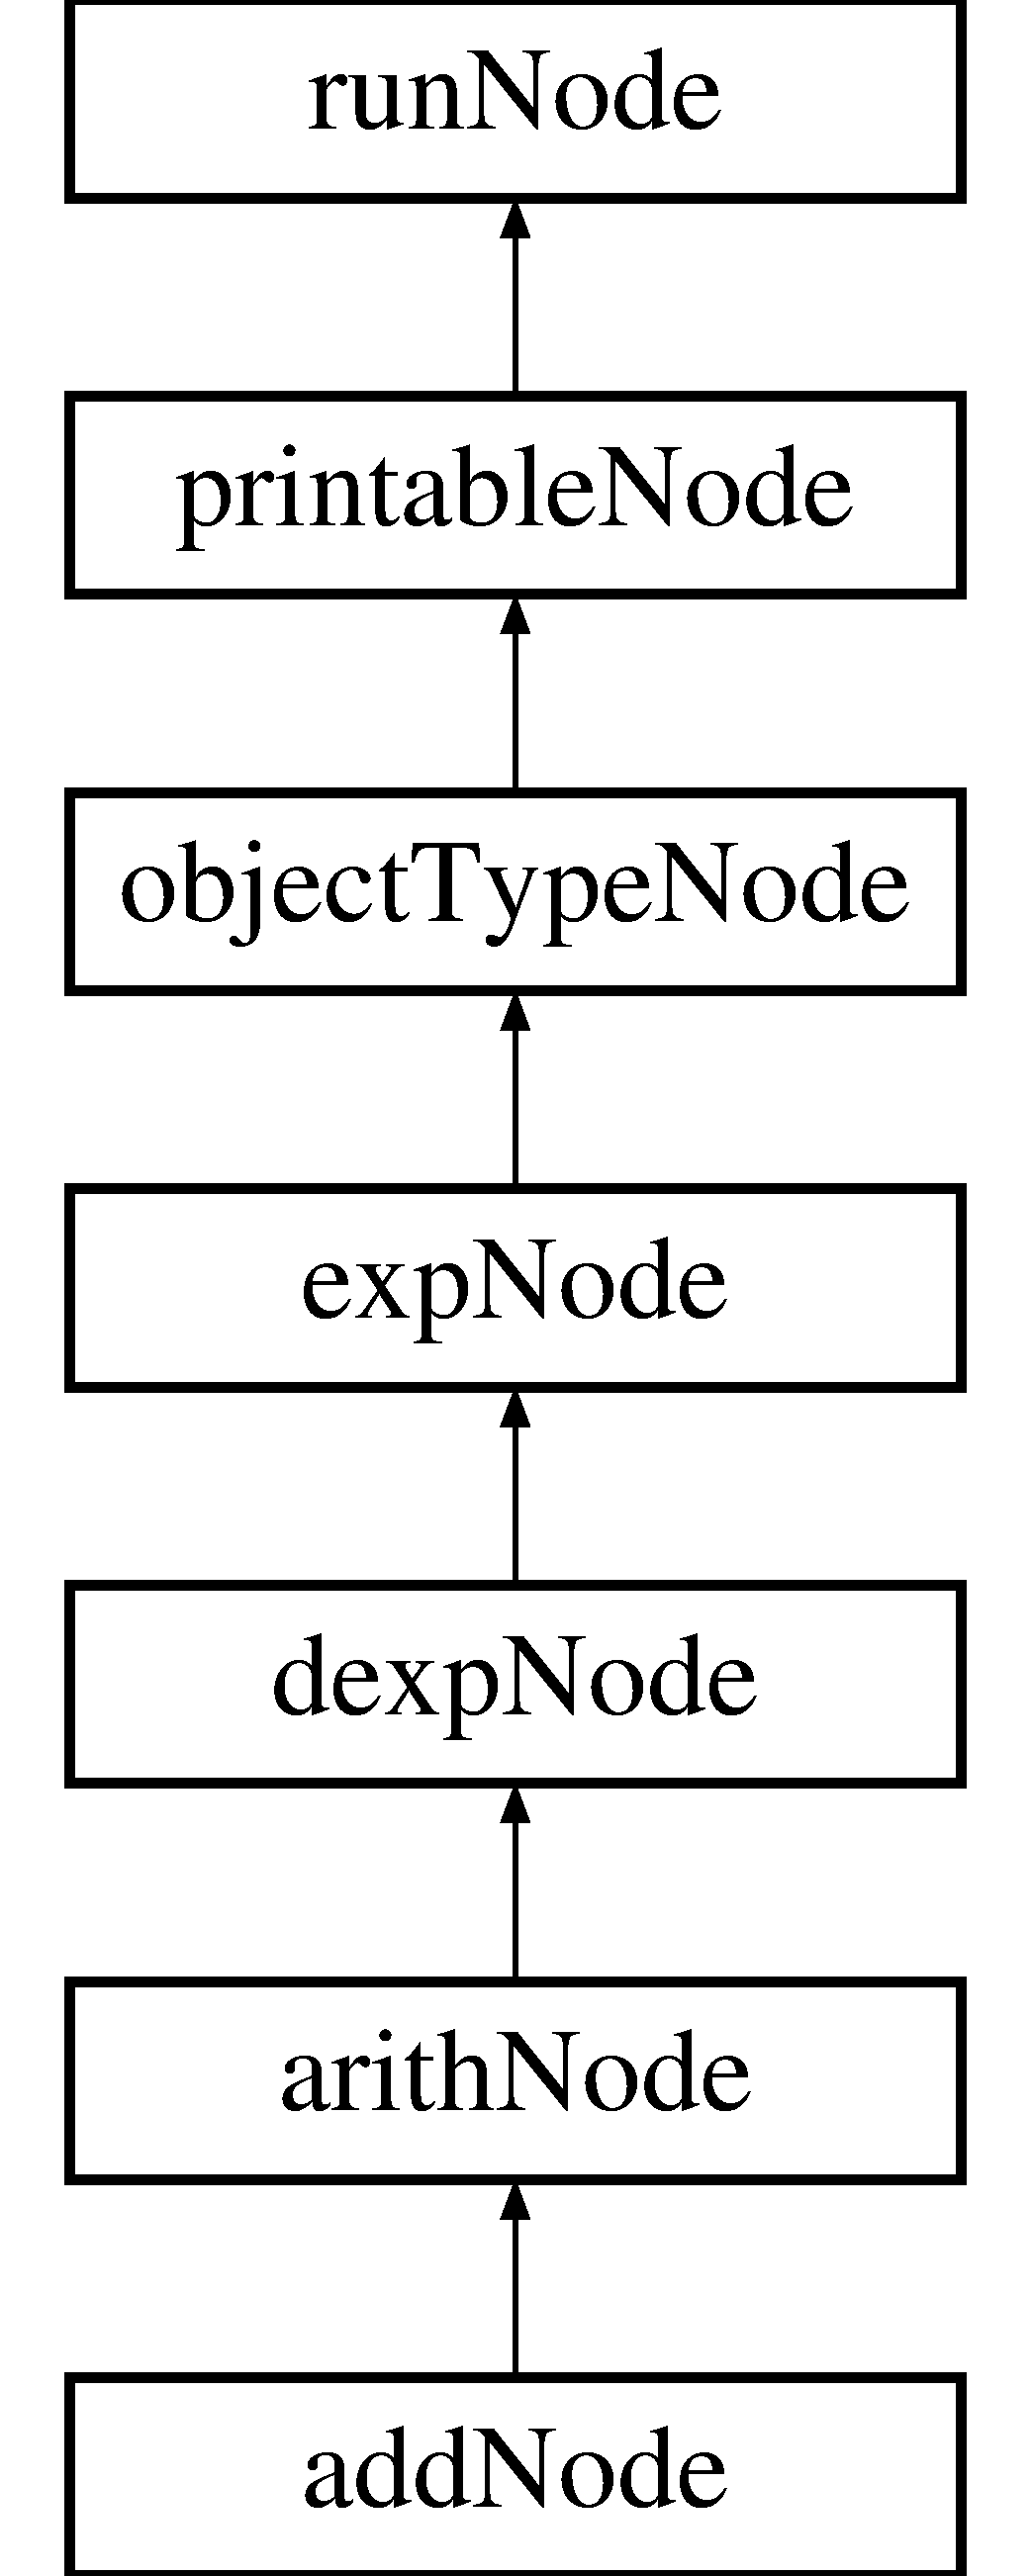
\includegraphics[height=7.000000cm]{classaddNode}
\end{center}
\end{figure}
\subsection*{Métodos públicos}
\begin{DoxyCompactItemize}
\item 
\hyperlink{classaddNode_a738f40ca4256c43bf0b7223b9c264ecb}{add\-Node} (\hyperlink{classrunNode}{run\-Node} $\ast$node1, \hyperlink{classrunNode}{run\-Node} $\ast$node2)
\item 
void \hyperlink{classaddNode_aade4eeee8fc992cc3322ee7f608ce5d2}{run} ()
\end{DoxyCompactItemize}
\subsection*{Métodos públicos estáticos}
\begin{DoxyCompactItemize}
\item 
static num \hyperlink{classaddNode_ae235f633dcf21852d3d9191c6a21fa97}{do\-\_\-add} (\hyperlink{classrunNode}{run\-Node} $\ast$op1, \hyperlink{classrunNode}{run\-Node} $\ast$op2)
\end{DoxyCompactItemize}
\subsection*{Otros miembros heredados}


\subsection{Descripción detallada}
Nodo operador suma. 

Este nodo implementa la operación suma sobre dos nodos asociados.

Si algún nodo es de tipo no aritmético fuerza la conversión a un tipo aritmético para realizar la operación.

El resultado de evaluar la expresión es un valor aritmético. 

\subsection{Documentación del constructor y destructor}
\hypertarget{classaddNode_a738f40ca4256c43bf0b7223b9c264ecb}{\index{add\-Node@{add\-Node}!add\-Node@{add\-Node}}
\index{add\-Node@{add\-Node}!addNode@{add\-Node}}
\subsubsection[{add\-Node}]{\setlength{\rightskip}{0pt plus 5cm}add\-Node\-::add\-Node (
\begin{DoxyParamCaption}
\item[{{\bf run\-Node} $\ast$}]{node1, }
\item[{{\bf run\-Node} $\ast$}]{node2}
\end{DoxyParamCaption}
)}}\label{classaddNode_a738f40ca4256c43bf0b7223b9c264ecb}
Constructor de la clase. Asocia el nodo operador a dos nodos. 
\begin{DoxyParams}{Parámetros}
{\em node1} & Primer nodo operando. \\
\hline
{\em node2} & Segundo nodo operando. \\
\hline
\end{DoxyParams}


\subsection{Documentación de las funciones miembro}
\hypertarget{classaddNode_ae235f633dcf21852d3d9191c6a21fa97}{\index{add\-Node@{add\-Node}!do\-\_\-add@{do\-\_\-add}}
\index{do\-\_\-add@{do\-\_\-add}!addNode@{add\-Node}}
\subsubsection[{do\-\_\-add}]{\setlength{\rightskip}{0pt plus 5cm}num add\-Node\-::do\-\_\-add (
\begin{DoxyParamCaption}
\item[{{\bf run\-Node} $\ast$}]{op1, }
\item[{{\bf run\-Node} $\ast$}]{op2}
\end{DoxyParamCaption}
)\hspace{0.3cm}{\ttfamily [static]}}}\label{classaddNode_ae235f633dcf21852d3d9191c6a21fa97}
Ejecuta la operación suma sobre dos nodos dados 
\begin{DoxyParams}{Parámetros}
{\em op1} & Primer nodo operando. \\
\hline
{\em op2} & Segundo nodo operando. \\
\hline
\end{DoxyParams}
\begin{DoxyReturn}{Devuelve}
Valor de la operación. 
\end{DoxyReturn}
\hypertarget{classaddNode_aade4eeee8fc992cc3322ee7f608ce5d2}{\index{add\-Node@{add\-Node}!run@{run}}
\index{run@{run}!addNode@{add\-Node}}
\subsubsection[{run}]{\setlength{\rightskip}{0pt plus 5cm}void add\-Node\-::run (
\begin{DoxyParamCaption}
{}
\end{DoxyParamCaption}
)\hspace{0.3cm}{\ttfamily [virtual]}}}\label{classaddNode_aade4eeee8fc992cc3322ee7f608ce5d2}
Método que ejecuta el nodo. Procede a la ejecución de los nodos asociados. Luego obtiene el valor aritmético del nodo mediante la operación suma entre el valor numérico de los dos nodos. 

Implementa \hyperlink{classrunNode_a83c10df8148829b08e04153c93d69eec}{run\-Node}.



La documentación para esta clase fue generada a partir de los siguientes ficheros\-:\begin{DoxyCompactItemize}
\item 
trunk/src/run/operators/\hyperlink{arithOpNode_8h}{arith\-Op\-Node.\-h}\item 
trunk/src/run/operators/arith\-Op\-Node.\-cpp\end{DoxyCompactItemize}

\hypertarget{classandNode}{\section{Referencia de la Clase and\-Node}
\label{classandNode}\index{and\-Node@{and\-Node}}
}


Nodo operador A\-N\-D.  




{\ttfamily \#include $<$logic\-Op\-Node.\-h$>$}

Diagrama de herencias de and\-Node\begin{figure}[H]
\begin{center}
\leavevmode
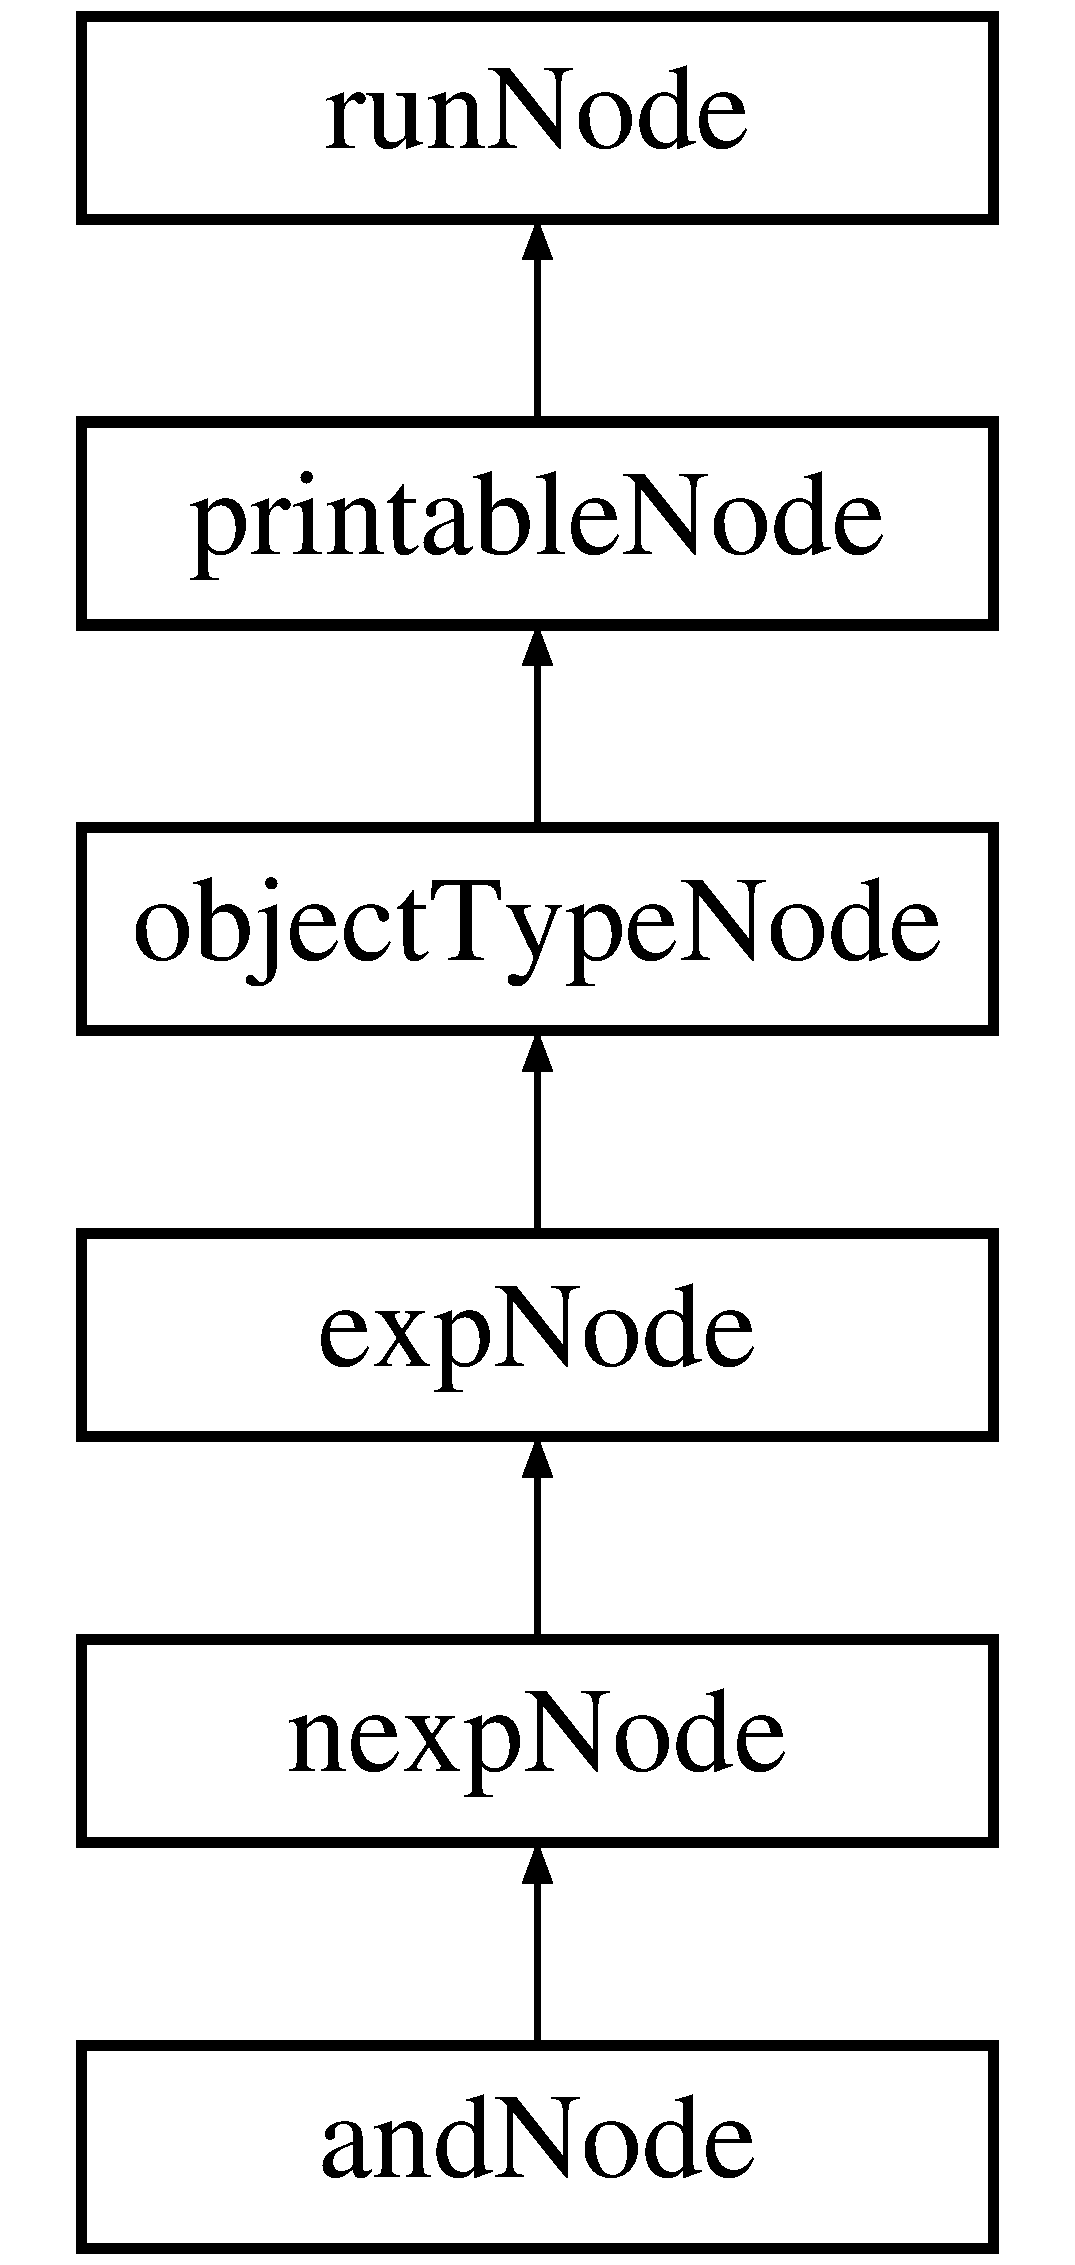
\includegraphics[height=6.000000cm]{classandNode}
\end{center}
\end{figure}
\subsection*{Métodos públicos}
\begin{DoxyCompactItemize}
\item 
\hyperlink{classandNode_acb6e360d4b21f6694813dba082a5670f}{and\-Node} (\hyperlink{classrunNode}{run\-Node} $\ast$op1, \hyperlink{classrunNode}{run\-Node} $\ast$op2)
\item 
void \hyperlink{classandNode_a87b7e06b52e72e4f6d08027d59310a7e}{run} ()
\item 
bool \hyperlink{classandNode_accc774b3bdd4c0a322b58a0947f06635}{do\-\_\-and} (\hyperlink{classrunNode}{run\-Node} $\ast$op1, \hyperlink{classrunNode}{run\-Node} $\ast$op2)
\end{DoxyCompactItemize}
\subsection*{Otros miembros heredados}


\subsection{Descripción detallada}
Nodo operador A\-N\-D. 

Este nodo implementa una operación lógica A\-N\-D entre dos nodos asociados.

Para llevar a cabo la operación lógica A\-N\-D se realiza una evaluación en cortocircuito, donde el valor del nodo A\-N\-D es el último valor evaluado. 

\subsection{Documentación del constructor y destructor}
\hypertarget{classandNode_acb6e360d4b21f6694813dba082a5670f}{\index{and\-Node@{and\-Node}!and\-Node@{and\-Node}}
\index{and\-Node@{and\-Node}!andNode@{and\-Node}}
\subsubsection[{and\-Node}]{\setlength{\rightskip}{0pt plus 5cm}and\-Node\-::and\-Node (
\begin{DoxyParamCaption}
\item[{{\bf run\-Node} $\ast$}]{op1, }
\item[{{\bf run\-Node} $\ast$}]{op2}
\end{DoxyParamCaption}
)}}\label{classandNode_acb6e360d4b21f6694813dba082a5670f}
Constructor de la clase. Asocia los nodos operandos. 
\begin{DoxyParams}{Parámetros}
{\em op1} & Primer nodo operando. \\
\hline
{\em op2} & Sengundo nodo operando. \\
\hline
\end{DoxyParams}


\subsection{Documentación de las funciones miembro}
\hypertarget{classandNode_accc774b3bdd4c0a322b58a0947f06635}{\index{and\-Node@{and\-Node}!do\-\_\-and@{do\-\_\-and}}
\index{do\-\_\-and@{do\-\_\-and}!andNode@{and\-Node}}
\subsubsection[{do\-\_\-and}]{\setlength{\rightskip}{0pt plus 5cm}bool and\-Node\-::do\-\_\-and (
\begin{DoxyParamCaption}
\item[{{\bf run\-Node} $\ast$}]{op1, }
\item[{{\bf run\-Node} $\ast$}]{op2}
\end{DoxyParamCaption}
)}}\label{classandNode_accc774b3bdd4c0a322b58a0947f06635}
Ejecuta la operación A\-N\-D entre dos nodos dados 
\begin{DoxyParams}{Parámetros}
{\em op1} & Primer nodo operando. \\
\hline
{\em op2} & Sengundo nodo operando. \\
\hline
\end{DoxyParams}
\begin{DoxyReturn}{Devuelve}
Valor de la operación 
\end{DoxyReturn}
\hypertarget{classandNode_a87b7e06b52e72e4f6d08027d59310a7e}{\index{and\-Node@{and\-Node}!run@{run}}
\index{run@{run}!andNode@{and\-Node}}
\subsubsection[{run}]{\setlength{\rightskip}{0pt plus 5cm}void and\-Node\-::run (
\begin{DoxyParamCaption}
{}
\end{DoxyParamCaption}
)\hspace{0.3cm}{\ttfamily [virtual]}}}\label{classandNode_a87b7e06b52e72e4f6d08027d59310a7e}
Función de ejecución. Procede a la ejecución de los nodos asociados. Toma como valor una referencia al último nodo evaluado según la operación A\-N\-D. 

Implementa \hyperlink{classrunNode_a83c10df8148829b08e04153c93d69eec}{run\-Node}.



La documentación para esta clase fue generada a partir de los siguientes ficheros\-:\begin{DoxyCompactItemize}
\item 
trunk/src/run/operators/\hyperlink{logicOpNode_8h}{logic\-Op\-Node.\-h}\item 
trunk/src/run/operators/logic\-Op\-Node.\-cpp\end{DoxyCompactItemize}

\hypertarget{classarithNode}{\section{Referencia de la Clase arith\-Node}
\label{classarithNode}\index{arith\-Node@{arith\-Node}}
}


Nodos aritméticos.  




{\ttfamily \#include $<$exp\-Node.\-h$>$}

Diagrama de herencias de arith\-Node\begin{figure}[H]
\begin{center}
\leavevmode
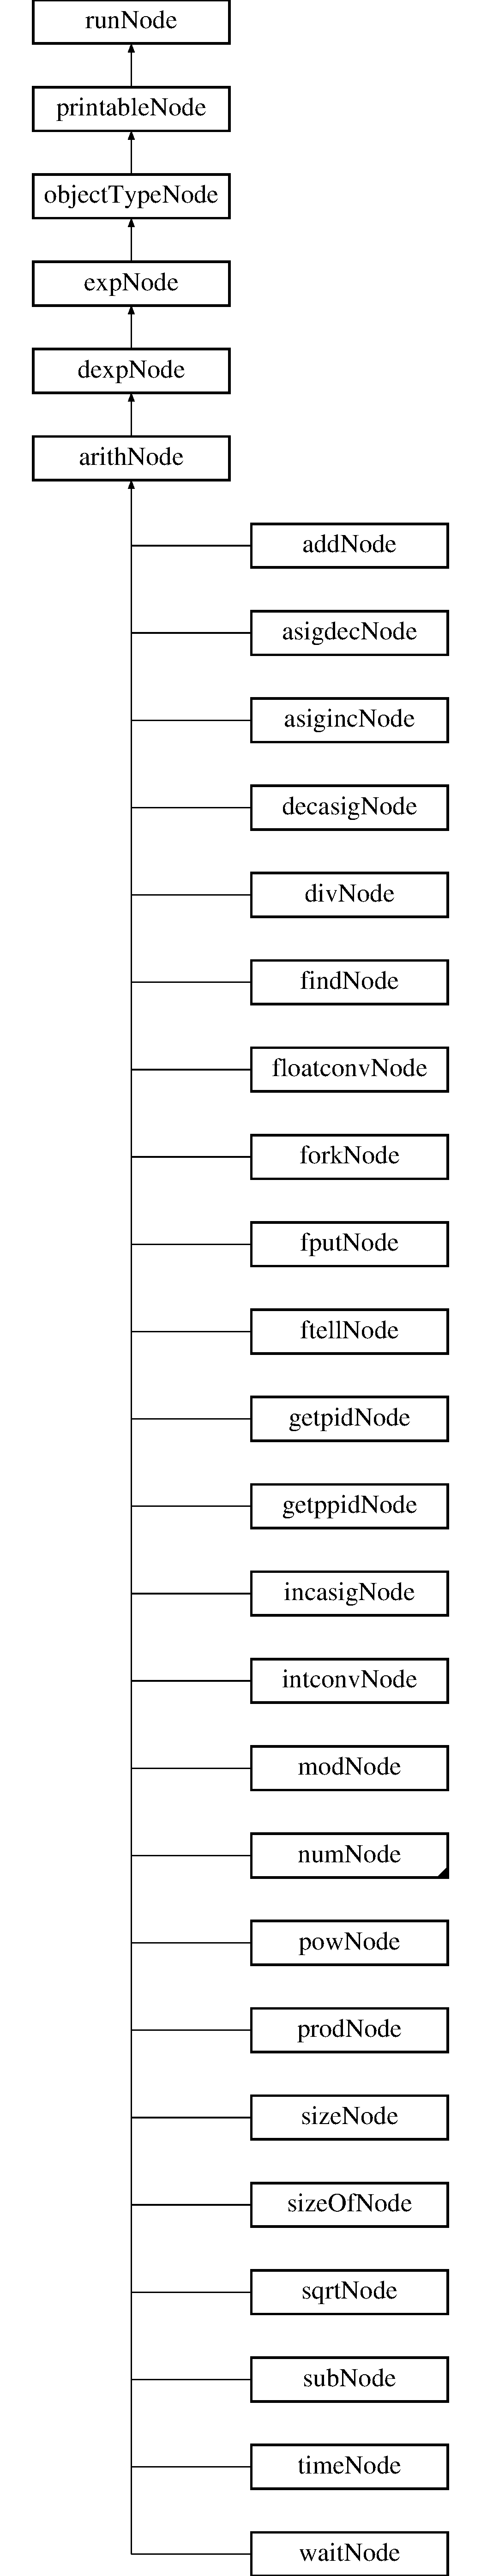
\includegraphics[height=12.000000cm]{classarithNode}
\end{center}
\end{figure}
\subsection*{Métodos públicos}
\begin{DoxyCompactItemize}
\item 
string \hyperlink{classarithNode_a8550d65d4f403ef6526bc7be240879b3}{print} () const 
\item 
\hyperlink{classrunNode}{run\-Node} $\ast$ \hyperlink{classarithNode_a5a8581334f3d1757085fb88278103dc9}{nodeval} () const 
\item 
num \hyperlink{classarithNode_a3914e65779e61750f1ffd528deabd120}{numvalue} () const 
\item 
bool \hyperlink{classarithNode_a7f3634eba193b245af5e3ba8081c017b}{boolvalue} () const 
\item 
string \hyperlink{classarithNode_a01f251d6cdc918309873c7443c694510}{strvalue} () const 
\item 
\hyperlink{classrunNode}{run\-Node} $\ast$ \hyperlink{classarithNode_a870a354180acd033140f1d2c2fcde5a6}{get\-Class} ()
\item 
virtual void \hyperlink{classarithNode_aa10435f1e329336baee9334df7a8b0cf}{set\-Node\-Value} (\hyperlink{classrunNode}{run\-Node} $\ast$node)
\end{DoxyCompactItemize}
\subsection*{Métodos públicos estáticos}
\begin{DoxyCompactItemize}
\item 
static num \hyperlink{classarithNode_a40e00712940d8de007c8fde31ff8837f}{to\-\_\-num} (\hyperlink{classrunNode}{run\-Node} $\ast$node, bool exception=true)
\item 
static void \hyperlink{classarithNode_a87b5618fdfee87decabfd1ec6aa1de51}{generate\-Class} ()
\end{DoxyCompactItemize}
\subsection*{Atributos protegidos}
\begin{DoxyCompactItemize}
\item 
num \hyperlink{classarithNode_a975a7d0704b4e450c6aaa2616dfc09e7}{numvalue\-\_\-}
\end{DoxyCompactItemize}


\subsection{Descripción detallada}
Nodos aritméticos. 

Los nodos aritméticos tienen un valor numérico asociado. Para la representación interna de un número se utiliza el tipo num que puede ser dado en tiempo de compilación. Normalmente este tipo contemplará los números que pueden ser representados por una expresión en coma flotante.

Todo nodo aritmético está asociado a un nodo clase \char`\"{}arith\-Class\char`\"{} 

\subsection{Documentación de las funciones miembro}
\hypertarget{classarithNode_a7f3634eba193b245af5e3ba8081c017b}{\index{arith\-Node@{arith\-Node}!boolvalue@{boolvalue}}
\index{boolvalue@{boolvalue}!arithNode@{arith\-Node}}
\subsubsection[{boolvalue}]{\setlength{\rightskip}{0pt plus 5cm}bool arith\-Node\-::boolvalue (
\begin{DoxyParamCaption}
{}
\end{DoxyParamCaption}
) const\hspace{0.3cm}{\ttfamily [virtual]}}}\label{classarithNode_a7f3634eba193b245af5e3ba8081c017b}
Convierte un nodo a su valor booleano. \begin{DoxyReturn}{Devuelve}
Valor booleano. 
\end{DoxyReturn}


Reimplementado de \hyperlink{classdexpNode_a18781e07cc3390c04b6905249755ccc8}{dexp\-Node}.

\hypertarget{classarithNode_a87b5618fdfee87decabfd1ec6aa1de51}{\index{arith\-Node@{arith\-Node}!generate\-Class@{generate\-Class}}
\index{generate\-Class@{generate\-Class}!arithNode@{arith\-Node}}
\subsubsection[{generate\-Class}]{\setlength{\rightskip}{0pt plus 5cm}void arith\-Node\-::generate\-Class (
\begin{DoxyParamCaption}
{}
\end{DoxyParamCaption}
)\hspace{0.3cm}{\ttfamily [static]}}}\label{classarithNode_a87b5618fdfee87decabfd1ec6aa1de51}
Genera la clase \char`\"{}arith\-Class\char`\"{} y la añade a la tabla de símbolos clases. \hypertarget{classarithNode_a870a354180acd033140f1d2c2fcde5a6}{\index{arith\-Node@{arith\-Node}!get\-Class@{get\-Class}}
\index{get\-Class@{get\-Class}!arithNode@{arith\-Node}}
\subsubsection[{get\-Class}]{\setlength{\rightskip}{0pt plus 5cm}{\bf run\-Node} $\ast$ arith\-Node\-::get\-Class (
\begin{DoxyParamCaption}
{}
\end{DoxyParamCaption}
)\hspace{0.3cm}{\ttfamily [virtual]}}}\label{classarithNode_a870a354180acd033140f1d2c2fcde5a6}
Obtienen el nodo clase asociado al nodo aritmético. \begin{DoxyReturn}{Devuelve}
Nodo clase. 
\end{DoxyReturn}


Reimplementado de \hyperlink{classobjectTypeNode_a42d4efaea6b650ef72807de94d3baa37}{object\-Type\-Node}.

\hypertarget{classarithNode_a5a8581334f3d1757085fb88278103dc9}{\index{arith\-Node@{arith\-Node}!nodeval@{nodeval}}
\index{nodeval@{nodeval}!arithNode@{arith\-Node}}
\subsubsection[{nodeval}]{\setlength{\rightskip}{0pt plus 5cm}{\bf run\-Node} $\ast$ arith\-Node\-::nodeval (
\begin{DoxyParamCaption}
{}
\end{DoxyParamCaption}
) const}}\label{classarithNode_a5a8581334f3d1757085fb88278103dc9}
Método que devuelve un nodo de tipo booleano con el mismo valor del nodo lógico. \begin{DoxyReturn}{Devuelve}
Nodo booleano. 
\end{DoxyReturn}
\hypertarget{classarithNode_a3914e65779e61750f1ffd528deabd120}{\index{arith\-Node@{arith\-Node}!numvalue@{numvalue}}
\index{numvalue@{numvalue}!arithNode@{arith\-Node}}
\subsubsection[{numvalue}]{\setlength{\rightskip}{0pt plus 5cm}num arith\-Node\-::numvalue (
\begin{DoxyParamCaption}
{}
\end{DoxyParamCaption}
) const\hspace{0.3cm}{\ttfamily [virtual]}}}\label{classarithNode_a3914e65779e61750f1ffd528deabd120}
Método observador que devuelve el valor numérico del nodo. \begin{DoxyReturn}{Devuelve}
Valor numérico del nodo. 
\end{DoxyReturn}


Reimplementado de \hyperlink{classdexpNode_ae2d3bfed7e6ebd5e96ddcefaa230c3d2}{dexp\-Node}.

\hypertarget{classarithNode_a8550d65d4f403ef6526bc7be240879b3}{\index{arith\-Node@{arith\-Node}!print@{print}}
\index{print@{print}!arithNode@{arith\-Node}}
\subsubsection[{print}]{\setlength{\rightskip}{0pt plus 5cm}string arith\-Node\-::print (
\begin{DoxyParamCaption}
{}
\end{DoxyParamCaption}
) const\hspace{0.3cm}{\ttfamily [virtual]}}}\label{classarithNode_a8550d65d4f403ef6526bc7be240879b3}
Devuelve la cadena de caracteres asociada al nodo que representa el valor numérico del mismo. \begin{DoxyReturn}{Devuelve}
Cadena de caracteres que representa el valor del nodo. 
\end{DoxyReturn}


Implementa \hyperlink{classprintableNode_ae5835e7b9d1a8af621723798137e01f9}{printable\-Node}.

\hypertarget{classarithNode_aa10435f1e329336baee9334df7a8b0cf}{\index{arith\-Node@{arith\-Node}!set\-Node\-Value@{set\-Node\-Value}}
\index{set\-Node\-Value@{set\-Node\-Value}!arithNode@{arith\-Node}}
\subsubsection[{set\-Node\-Value}]{\setlength{\rightskip}{0pt plus 5cm}void arith\-Node\-::set\-Node\-Value (
\begin{DoxyParamCaption}
\item[{{\bf run\-Node} $\ast$}]{node}
\end{DoxyParamCaption}
)\hspace{0.3cm}{\ttfamily [virtual]}}}\label{classarithNode_aa10435f1e329336baee9334df7a8b0cf}
Establece el valor del nodo a partir de otro nodo. 
\begin{DoxyParams}{Parámetros}
{\em node} & Nodo a partir del cual se tomará el valor. \\
\hline
\end{DoxyParams}


Reimplementado de \hyperlink{classexpNode_aedb96104889212bae315a6381f8e0219}{exp\-Node}.

\hypertarget{classarithNode_a01f251d6cdc918309873c7443c694510}{\index{arith\-Node@{arith\-Node}!strvalue@{strvalue}}
\index{strvalue@{strvalue}!arithNode@{arith\-Node}}
\subsubsection[{strvalue}]{\setlength{\rightskip}{0pt plus 5cm}string arith\-Node\-::strvalue (
\begin{DoxyParamCaption}
{}
\end{DoxyParamCaption}
) const\hspace{0.3cm}{\ttfamily [virtual]}}}\label{classarithNode_a01f251d6cdc918309873c7443c694510}
Convierte un nodo a su valor cadena de caracteres. \begin{DoxyReturn}{Devuelve}
Valor cadena de caracteres. 
\end{DoxyReturn}


Reimplementado de \hyperlink{classdexpNode_adf74f4f848f7ec7c3c2ada1aa3bdc66d}{dexp\-Node}.

\hypertarget{classarithNode_a40e00712940d8de007c8fde31ff8837f}{\index{arith\-Node@{arith\-Node}!to\-\_\-num@{to\-\_\-num}}
\index{to\-\_\-num@{to\-\_\-num}!arithNode@{arith\-Node}}
\subsubsection[{to\-\_\-num}]{\setlength{\rightskip}{0pt plus 5cm}num arith\-Node\-::to\-\_\-num (
\begin{DoxyParamCaption}
\item[{{\bf run\-Node} $\ast$}]{node, }
\item[{bool}]{exception = {\ttfamily true}}
\end{DoxyParamCaption}
)\hspace{0.3cm}{\ttfamily [static]}}}\label{classarithNode_a40e00712940d8de007c8fde31ff8837f}
Convierte un nodo a su valor aritmético. \begin{DoxyReturn}{Devuelve}
Valor numérico. 
\end{DoxyReturn}


\subsection{Documentación de los datos miembro}
\hypertarget{classarithNode_a975a7d0704b4e450c6aaa2616dfc09e7}{\index{arith\-Node@{arith\-Node}!numvalue\-\_\-@{numvalue\-\_\-}}
\index{numvalue\-\_\-@{numvalue\-\_\-}!arithNode@{arith\-Node}}
\subsubsection[{numvalue\-\_\-}]{\setlength{\rightskip}{0pt plus 5cm}num arith\-Node\-::numvalue\-\_\-\hspace{0.3cm}{\ttfamily [protected]}}}\label{classarithNode_a975a7d0704b4e450c6aaa2616dfc09e7}
Atributo que representa el valor numérico del nodo. 

La documentación para esta clase fue generada a partir de los siguientes ficheros\-:\begin{DoxyCompactItemize}
\item 
trunk/src/run/tree/\hyperlink{expNode_8h}{exp\-Node.\-h}\item 
trunk/src/run/tree/exp\-Node.\-cpp\end{DoxyCompactItemize}

\hypertarget{classarrayChunkNode}{\section{Referencia de la Clase array\-Chunk\-Node}
\label{classarrayChunkNode}\index{array\-Chunk\-Node@{array\-Chunk\-Node}}
}


Nodo division de array.  




{\ttfamily \#include $<$array\-Op\-Node.\-h$>$}

Diagrama de herencias de array\-Chunk\-Node\begin{figure}[H]
\begin{center}
\leavevmode
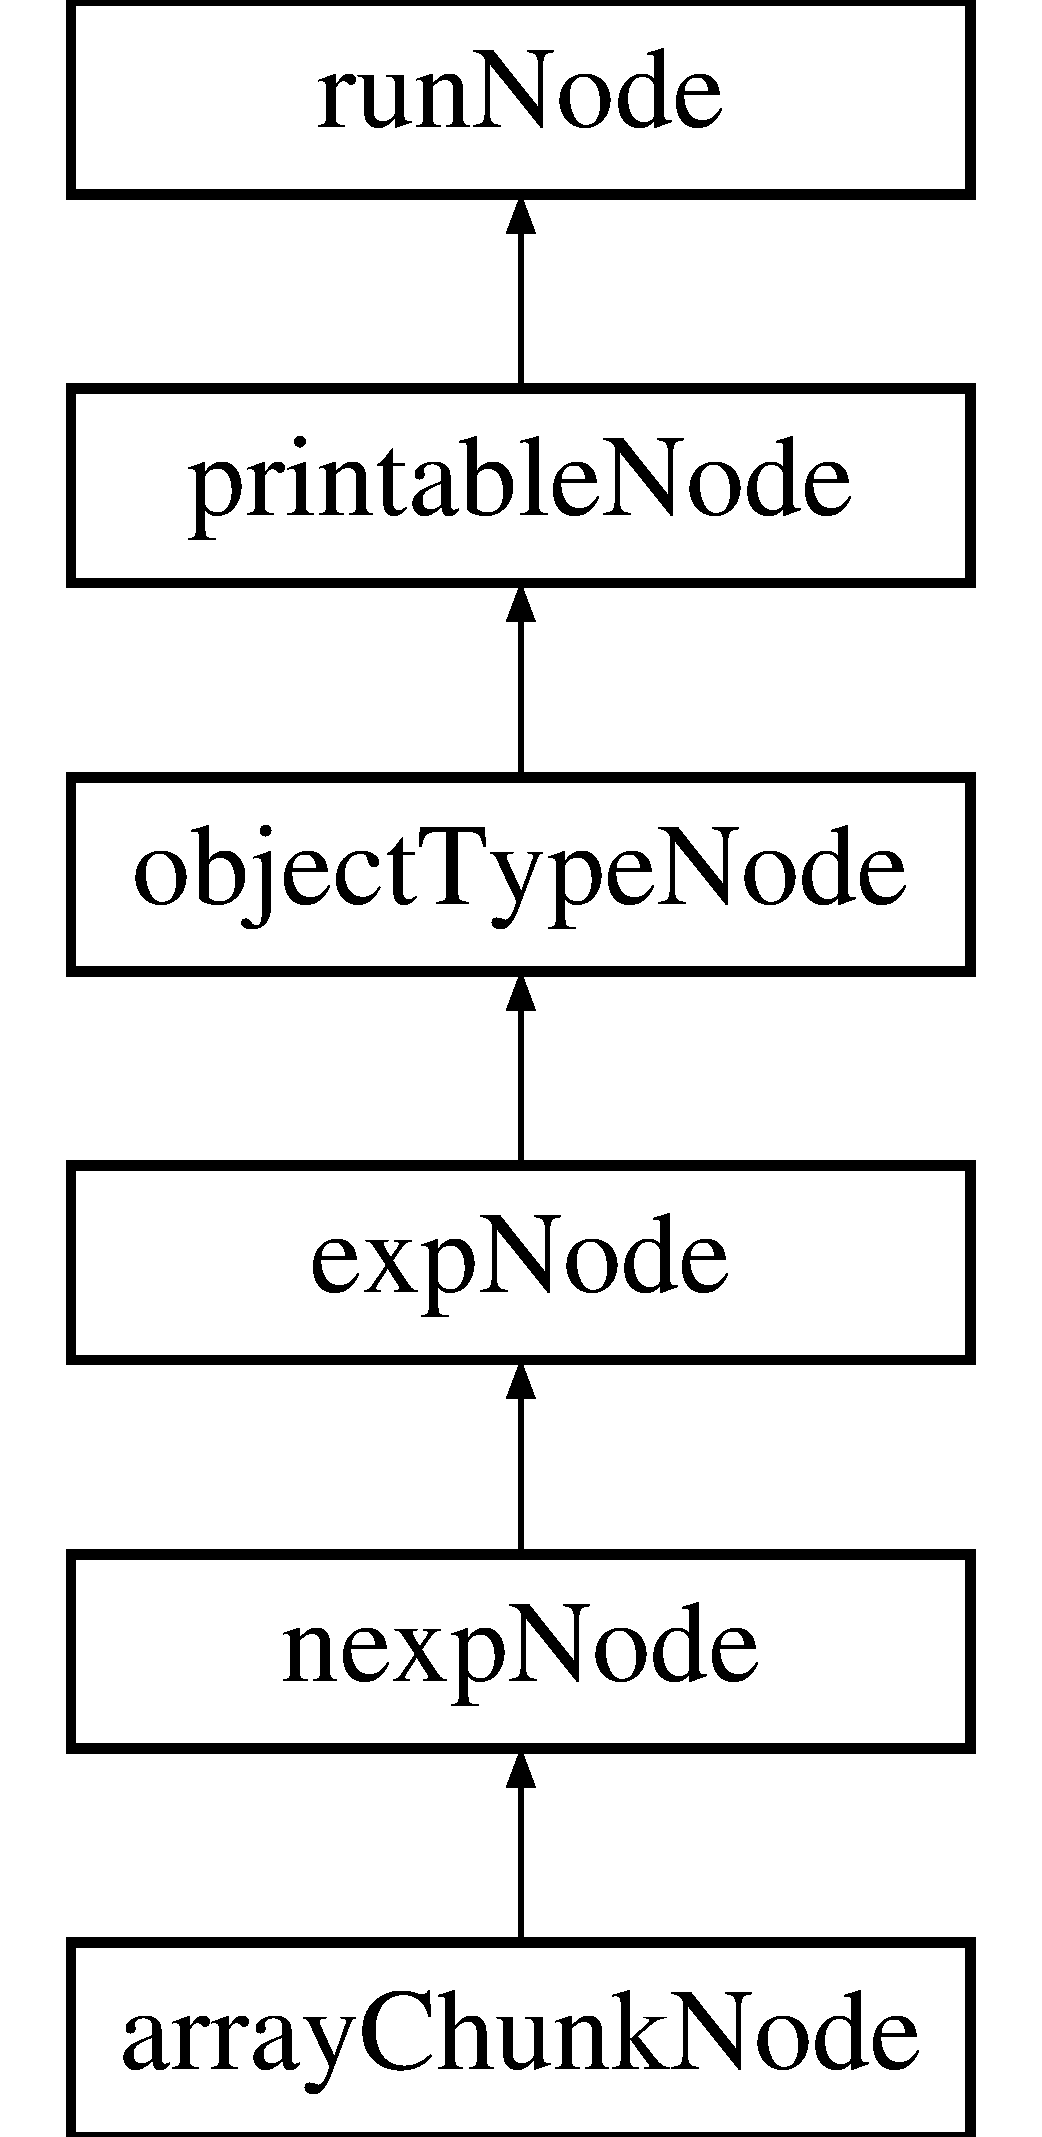
\includegraphics[height=6.000000cm]{classarrayChunkNode}
\end{center}
\end{figure}
\subsection*{Métodos públicos}
\begin{DoxyCompactItemize}
\item 
\hyperlink{classarrayChunkNode_a2f1eb4437b5ac66ccd8909af51fc8ec8}{array\-Chunk\-Node} (\hyperlink{classrunNode}{run\-Node} $\ast$array, \hyperlink{classrunNode}{run\-Node} $\ast$size)
\item 
void \hyperlink{classarrayChunkNode_afaeae0c90a08aa29b23ff3852a089489}{run} ()
\end{DoxyCompactItemize}
\subsection*{Métodos públicos estáticos}
\begin{DoxyCompactItemize}
\item 
static \hyperlink{classrunNode}{run\-Node} $\ast$ \hyperlink{classarrayChunkNode_a7b458328d01121dcaf5d432e37972c3a}{as\-Method} ()
\end{DoxyCompactItemize}


\subsection{Descripción detallada}
Nodo division de array. 

Nodo cuya ejecución consiste en la división de un array en varios fragmentos determinados por un tamaño 

\subsection{Documentación del constructor y destructor}
\hypertarget{classarrayChunkNode_a2f1eb4437b5ac66ccd8909af51fc8ec8}{\index{array\-Chunk\-Node@{array\-Chunk\-Node}!array\-Chunk\-Node@{array\-Chunk\-Node}}
\index{array\-Chunk\-Node@{array\-Chunk\-Node}!arrayChunkNode@{array\-Chunk\-Node}}
\subsubsection[{array\-Chunk\-Node}]{\setlength{\rightskip}{0pt plus 5cm}array\-Chunk\-Node\-::array\-Chunk\-Node (
\begin{DoxyParamCaption}
\item[{{\bf run\-Node} $\ast$}]{array, }
\item[{{\bf run\-Node} $\ast$}]{size}
\end{DoxyParamCaption}
)}}\label{classarrayChunkNode_a2f1eb4437b5ac66ccd8909af51fc8ec8}
Constructor de la clase. Este nodo se inicializa a partir de un array y el tamaño de cada fragmento. 
\begin{DoxyParams}{Parámetros}
{\em array} & Nodo que hace de Array \\
\hline
{\em size} & Nodo que hace de tamaño \\
\hline
\end{DoxyParams}


\subsection{Documentación de las funciones miembro}
\hypertarget{classarrayChunkNode_a7b458328d01121dcaf5d432e37972c3a}{\index{array\-Chunk\-Node@{array\-Chunk\-Node}!as\-Method@{as\-Method}}
\index{as\-Method@{as\-Method}!arrayChunkNode@{array\-Chunk\-Node}}
\subsubsection[{as\-Method}]{\setlength{\rightskip}{0pt plus 5cm}{\bf run\-Node} $\ast$ array\-Chunk\-Node\-::as\-Method (
\begin{DoxyParamCaption}
{}
\end{DoxyParamCaption}
)\hspace{0.3cm}{\ttfamily [static]}}}\label{classarrayChunkNode_a7b458328d01121dcaf5d432e37972c3a}
Devuelve un nodo división de array como cuerpo de un nodo función, siendo un nodo this el array de elementos. \begin{DoxyReturn}{Devuelve}
Método chunk. 
\end{DoxyReturn}
\hypertarget{classarrayChunkNode_afaeae0c90a08aa29b23ff3852a089489}{\index{array\-Chunk\-Node@{array\-Chunk\-Node}!run@{run}}
\index{run@{run}!arrayChunkNode@{array\-Chunk\-Node}}
\subsubsection[{run}]{\setlength{\rightskip}{0pt plus 5cm}void array\-Chunk\-Node\-::run (
\begin{DoxyParamCaption}
{}
\end{DoxyParamCaption}
)\hspace{0.3cm}{\ttfamily [virtual]}}}\label{classarrayChunkNode_afaeae0c90a08aa29b23ff3852a089489}
Método que ejecuta el nodo. Se encarga de dividir el array de elementos en varios fragmentos segun el tamaño dado. Toma como valor otro array cuyos elementos son cada uno de los fragmentos. 

Implementa \hyperlink{classrunNode_a83c10df8148829b08e04153c93d69eec}{run\-Node}.



La documentación para esta clase fue generada a partir de los siguientes ficheros\-:\begin{DoxyCompactItemize}
\item 
trunk/src/run/operators/\hyperlink{arrayOpNode_8h}{array\-Op\-Node.\-h}\item 
trunk/src/run/operators/array\-Op\-Node.\-cpp\end{DoxyCompactItemize}

\hypertarget{classarrayConstNode}{\section{Referencia de la Clase array\-Const\-Node}
\label{classarrayConstNode}\index{array\-Const\-Node@{array\-Const\-Node}}
}


Nodo array constante.  




{\ttfamily \#include $<$type\-Node.\-h$>$}

Diagrama de herencias de array\-Const\-Node\begin{figure}[H]
\begin{center}
\leavevmode
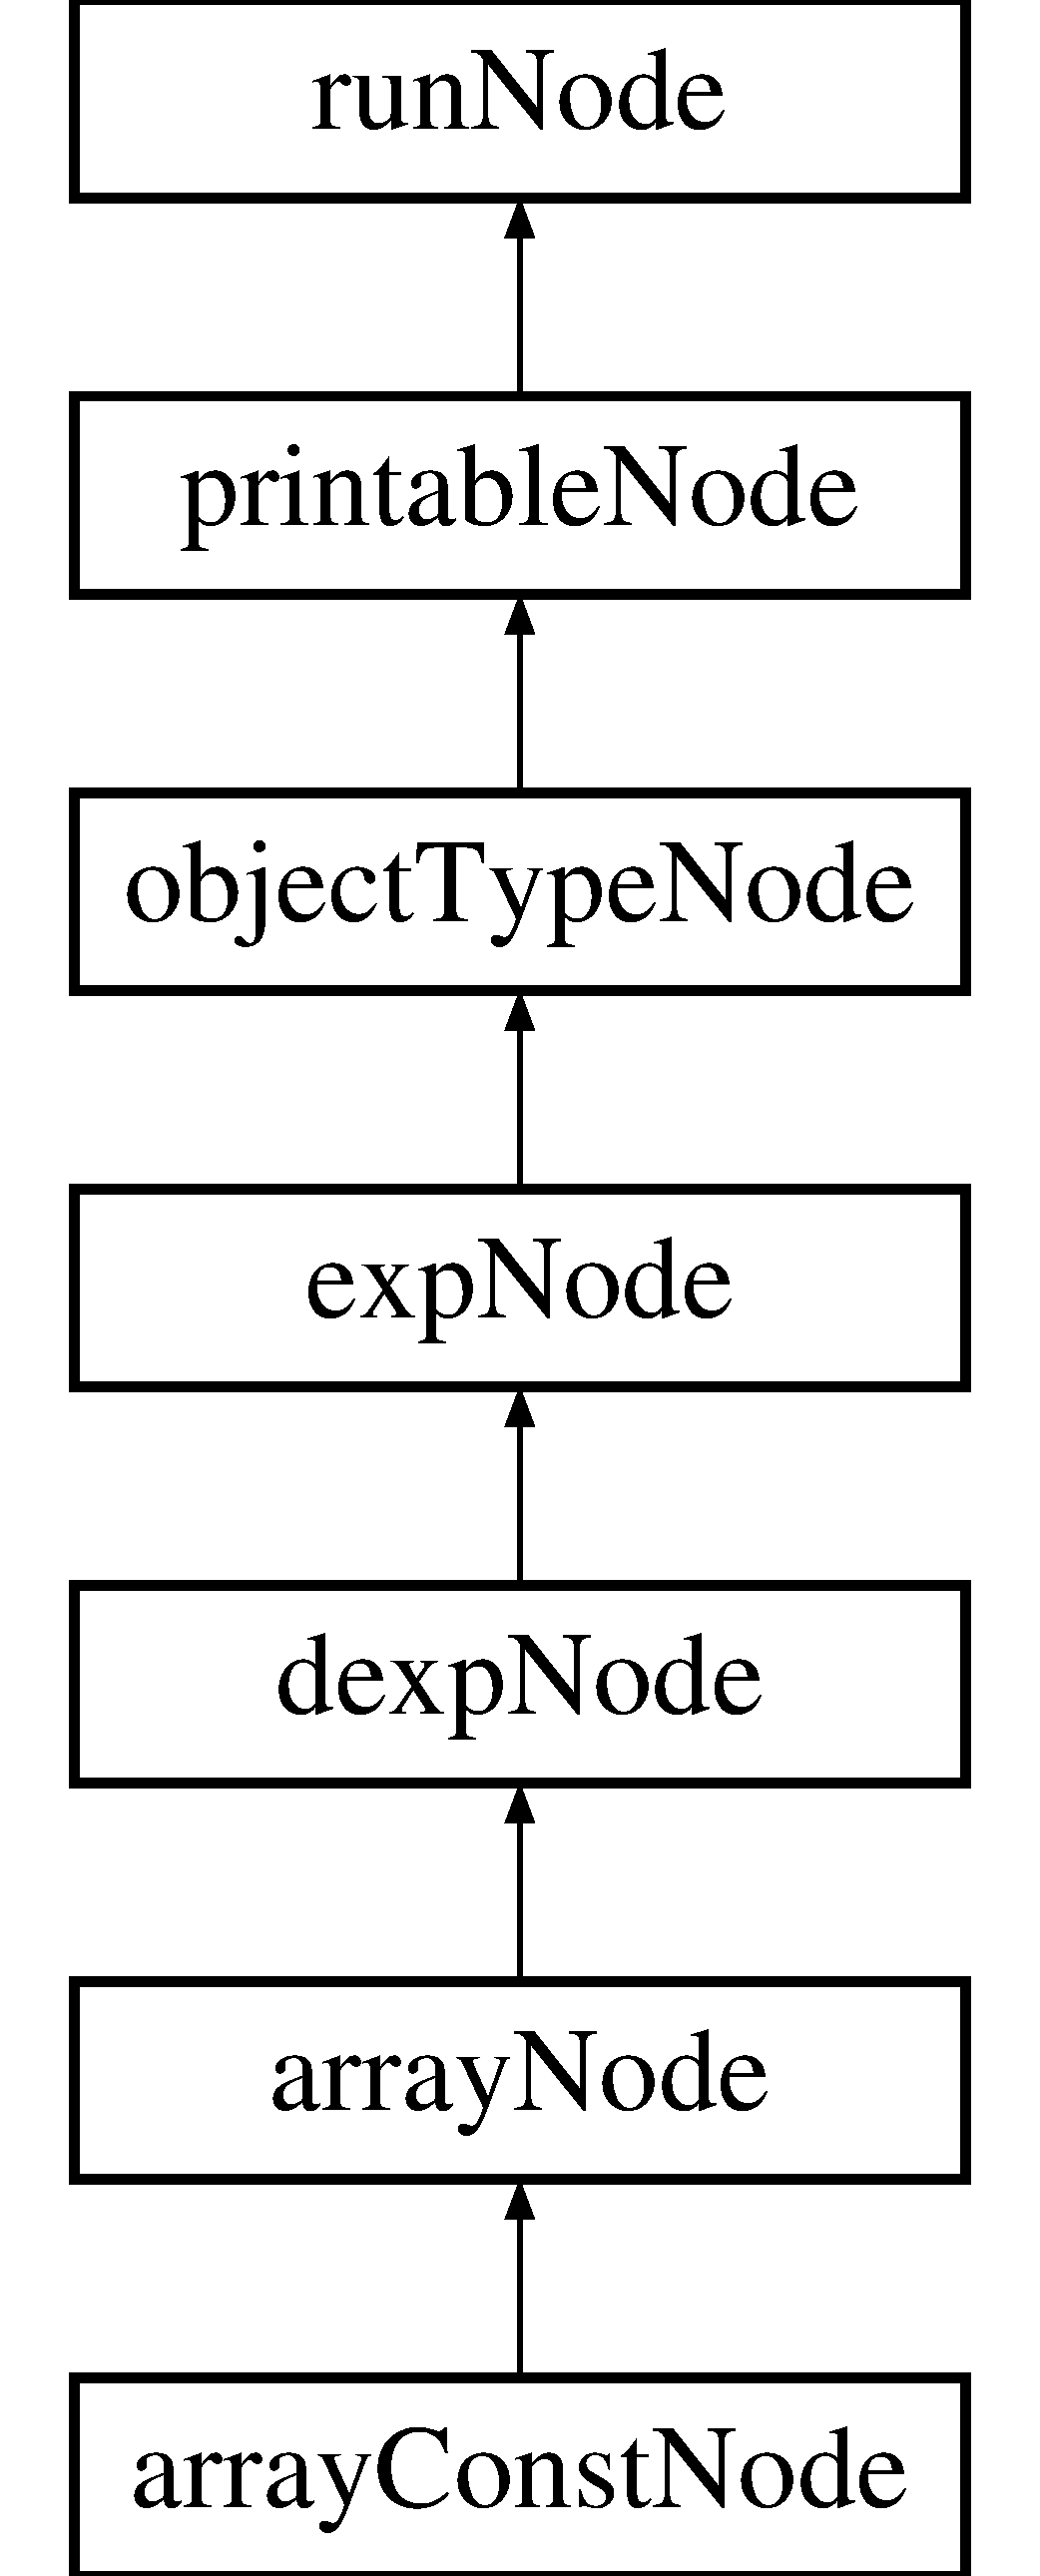
\includegraphics[height=7.000000cm]{classarrayConstNode}
\end{center}
\end{figure}
\subsection*{Métodos públicos}
\begin{DoxyCompactItemize}
\item 
\hyperlink{classarrayConstNode_a6032c2b8e43345e5198e1331ec64d729}{array\-Const\-Node} (\hyperlink{classlistNode}{list\-Node} $\ast$list)
\item 
void \hyperlink{classarrayConstNode_a84b4ae603b7c24d96f16a8acc94a0403}{run} ()
\item 
void \hyperlink{classarrayConstNode_a93fccf8c5a3fa33313a21b8e3e8838f0}{rm\-Ref} ()
\item 
void \hyperlink{classarrayConstNode_aba71d93899fadd2d756009ce16f5eefc}{is\-Cloned} (bool cloned)
\end{DoxyCompactItemize}
\subsection*{Otros miembros heredados}


\subsection{Descripción detallada}
Nodo array constante. 

Un nodo constante sobrecarga el método de eliminar referencia para que no pueda ser elimado de la forma normal. 

\subsection{Documentación del constructor y destructor}
\hypertarget{classarrayConstNode_a6032c2b8e43345e5198e1331ec64d729}{\index{array\-Const\-Node@{array\-Const\-Node}!array\-Const\-Node@{array\-Const\-Node}}
\index{array\-Const\-Node@{array\-Const\-Node}!arrayConstNode@{array\-Const\-Node}}
\subsubsection[{array\-Const\-Node}]{\setlength{\rightskip}{0pt plus 5cm}array\-Const\-Node\-::array\-Const\-Node (
\begin{DoxyParamCaption}
\item[{{\bf list\-Node} $\ast$}]{list}
\end{DoxyParamCaption}
)}}\label{classarrayConstNode_a6032c2b8e43345e5198e1331ec64d729}
Constructor de la clase. 
\begin{DoxyParams}{Parámetros}
{\em data} & Valor lista del nodo. \\
\hline
\end{DoxyParams}


\subsection{Documentación de las funciones miembro}
\hypertarget{classarrayConstNode_aba71d93899fadd2d756009ce16f5eefc}{\index{array\-Const\-Node@{array\-Const\-Node}!is\-Cloned@{is\-Cloned}}
\index{is\-Cloned@{is\-Cloned}!arrayConstNode@{array\-Const\-Node}}
\subsubsection[{is\-Cloned}]{\setlength{\rightskip}{0pt plus 5cm}void array\-Const\-Node\-::is\-Cloned (
\begin{DoxyParamCaption}
\item[{bool}]{cloned}
\end{DoxyParamCaption}
)\hspace{0.3cm}{\ttfamily [inline]}}}\label{classarrayConstNode_aba71d93899fadd2d756009ce16f5eefc}
Establece si el nodo ha sido clonado. 
\begin{DoxyParams}{Parámetros}
{\em cloned} & Determinará si el nodo fue clonado. \\
\hline
\end{DoxyParams}
\hypertarget{classarrayConstNode_a93fccf8c5a3fa33313a21b8e3e8838f0}{\index{array\-Const\-Node@{array\-Const\-Node}!rm\-Ref@{rm\-Ref}}
\index{rm\-Ref@{rm\-Ref}!arrayConstNode@{array\-Const\-Node}}
\subsubsection[{rm\-Ref}]{\setlength{\rightskip}{0pt plus 5cm}void array\-Const\-Node\-::rm\-Ref (
\begin{DoxyParamCaption}
{}
\end{DoxyParamCaption}
)\hspace{0.3cm}{\ttfamily [virtual]}}}\label{classarrayConstNode_a93fccf8c5a3fa33313a21b8e3e8838f0}
Sobrecarga del método para eliminar referencias. 

Reimplementado de \hyperlink{classrunNode_a8d0761660753ceb2c98836614c526a45}{run\-Node}.

\hypertarget{classarrayConstNode_a84b4ae603b7c24d96f16a8acc94a0403}{\index{array\-Const\-Node@{array\-Const\-Node}!run@{run}}
\index{run@{run}!arrayConstNode@{array\-Const\-Node}}
\subsubsection[{run}]{\setlength{\rightskip}{0pt plus 5cm}void array\-Const\-Node\-::run (
\begin{DoxyParamCaption}
{}
\end{DoxyParamCaption}
)\hspace{0.3cm}{\ttfamily [virtual]}}}\label{classarrayConstNode_a84b4ae603b7c24d96f16a8acc94a0403}
La ejecución de un array consiste en recorrer la lista de elementos asociadas al mismo y guardarlos en la tabla de símbolos. 

Reimplementado de \hyperlink{classarrayNode_a5ead9863a0f9478798c7777a0c03b1a5}{array\-Node}.



La documentación para esta clase fue generada a partir de los siguientes ficheros\-:\begin{DoxyCompactItemize}
\item 
trunk/src/run/tree/\hyperlink{typeNode_8h}{type\-Node.\-h}\item 
trunk/src/run/tree/\hyperlink{typeNode_8cpp}{type\-Node.\-cpp}\end{DoxyCompactItemize}

\hypertarget{classarraydeleteNode}{\section{Referencia de la Clase arraydelete\-Node}
\label{classarraydeleteNode}\index{arraydelete\-Node@{arraydelete\-Node}}
}


Nodo función eliminar elemento de array.  




{\ttfamily \#include $<$array\-Op\-Node.\-h$>$}

Diagrama de herencias de arraydelete\-Node\begin{figure}[H]
\begin{center}
\leavevmode
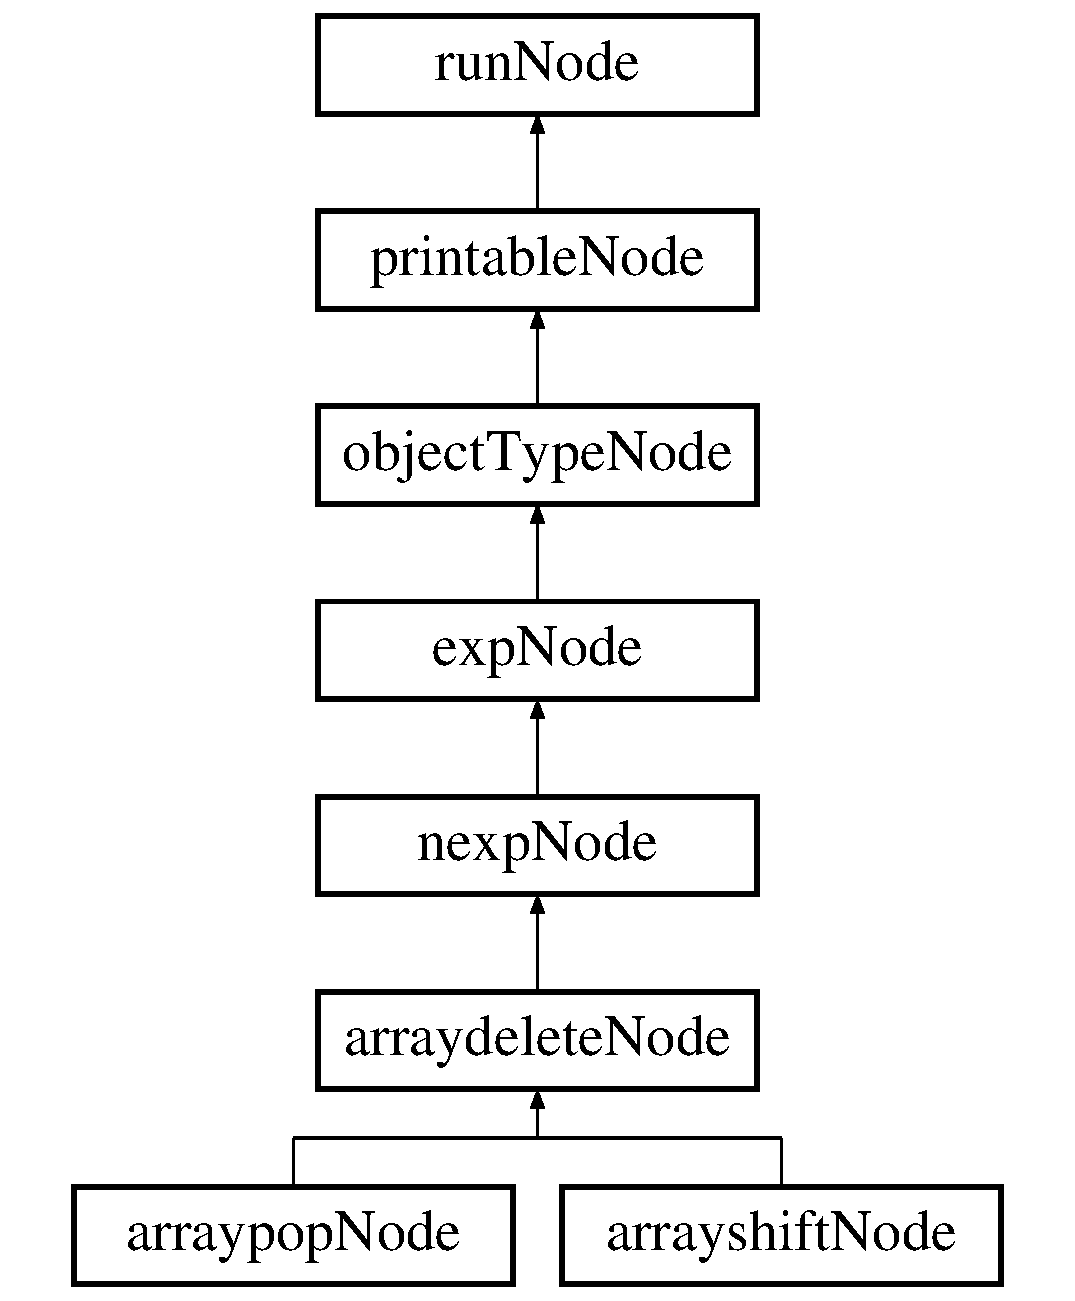
\includegraphics[height=7.000000cm]{classarraydeleteNode}
\end{center}
\end{figure}
\subsection*{Métodos públicos}
\begin{DoxyCompactItemize}
\item 
\hyperlink{classarraydeleteNode_abd17e65ebd9704157cb3f431f3dbcf97}{arraydelete\-Node} (\hyperlink{classrunNode}{run\-Node} $\ast$array, \hyperlink{classrunNode}{run\-Node} $\ast$index)
\item 
void \hyperlink{classarraydeleteNode_a0ce9f89cbb1485472f071b3573f0477d}{run} ()
\end{DoxyCompactItemize}
\subsection*{Métodos públicos estáticos}
\begin{DoxyCompactItemize}
\item 
static \hyperlink{classrunNode}{run\-Node} $\ast$ \hyperlink{classarraydeleteNode_a31ba9b73f9e6266042779eb8b8bffb01}{as\-Method} ()
\end{DoxyCompactItemize}


\subsection{Descripción detallada}
Nodo función eliminar elemento de array. 

Este nodo se encarga de eliminar el elemento que ocupa una determinada posición dentro de un array. Si la posición se encuentra fuera de rango se produce un error. 

\subsection{Documentación del constructor y destructor}
\hypertarget{classarraydeleteNode_abd17e65ebd9704157cb3f431f3dbcf97}{\index{arraydelete\-Node@{arraydelete\-Node}!arraydelete\-Node@{arraydelete\-Node}}
\index{arraydelete\-Node@{arraydelete\-Node}!arraydeleteNode@{arraydelete\-Node}}
\subsubsection[{arraydelete\-Node}]{\setlength{\rightskip}{0pt plus 5cm}arraydelete\-Node\-::arraydelete\-Node (
\begin{DoxyParamCaption}
\item[{{\bf run\-Node} $\ast$}]{array, }
\item[{{\bf run\-Node} $\ast$}]{index}
\end{DoxyParamCaption}
)}}\label{classarraydeleteNode_abd17e65ebd9704157cb3f431f3dbcf97}
Constructor de la clase 
\begin{DoxyParams}{Parámetros}
{\em array} & Nodo que representa el array \\
\hline
{\em index} & Nodo que representa la posición \\
\hline
\end{DoxyParams}


\subsection{Documentación de las funciones miembro}
\hypertarget{classarraydeleteNode_a31ba9b73f9e6266042779eb8b8bffb01}{\index{arraydelete\-Node@{arraydelete\-Node}!as\-Method@{as\-Method}}
\index{as\-Method@{as\-Method}!arraydeleteNode@{arraydelete\-Node}}
\subsubsection[{as\-Method}]{\setlength{\rightskip}{0pt plus 5cm}{\bf run\-Node} $\ast$ arraydelete\-Node\-::as\-Method (
\begin{DoxyParamCaption}
{}
\end{DoxyParamCaption}
)\hspace{0.3cm}{\ttfamily [static]}}}\label{classarraydeleteNode_a31ba9b73f9e6266042779eb8b8bffb01}
Devuelve un nodo eliminar elemento de array como cuerpo de un nodo función, siendo un nodo this el array de elementos. \begin{DoxyReturn}{Devuelve}
Método delete. 
\end{DoxyReturn}
\hypertarget{classarraydeleteNode_a0ce9f89cbb1485472f071b3573f0477d}{\index{arraydelete\-Node@{arraydelete\-Node}!run@{run}}
\index{run@{run}!arraydeleteNode@{arraydelete\-Node}}
\subsubsection[{run}]{\setlength{\rightskip}{0pt plus 5cm}void arraydelete\-Node\-::run (
\begin{DoxyParamCaption}
{}
\end{DoxyParamCaption}
)\hspace{0.3cm}{\ttfamily [virtual]}}}\label{classarraydeleteNode_a0ce9f89cbb1485472f071b3573f0477d}
Método que ejecuta el nodo. Elimina el elemento que ocuapa la posición dada dentro del array. Toma como valor una referencia al array con el elemento eliminado. 

Implementa \hyperlink{classrunNode_a83c10df8148829b08e04153c93d69eec}{run\-Node}.



Reimplementado en \hyperlink{classarraypopNode_a5a96f6ab8867ca653bbe74ec8f4c1d4b}{arraypop\-Node} y \hyperlink{classarrayshiftNode_a2a34028d6f0763c7df0220ef2c624580}{arrayshift\-Node}.



La documentación para esta clase fue generada a partir de los siguientes ficheros\-:\begin{DoxyCompactItemize}
\item 
trunk/src/run/operators/\hyperlink{arrayOpNode_8h}{array\-Op\-Node.\-h}\item 
trunk/src/run/operators/array\-Op\-Node.\-cpp\end{DoxyCompactItemize}

\hypertarget{classarrayfirstNode}{\section{Referencia de la Clase arrayfirst\-Node}
\label{classarrayfirstNode}\index{arrayfirst\-Node@{arrayfirst\-Node}}
}


Nodo función priemer elemento de array.  




{\ttfamily \#include $<$array\-Op\-Node.\-h$>$}

Diagrama de herencias de arrayfirst\-Node\begin{figure}[H]
\begin{center}
\leavevmode
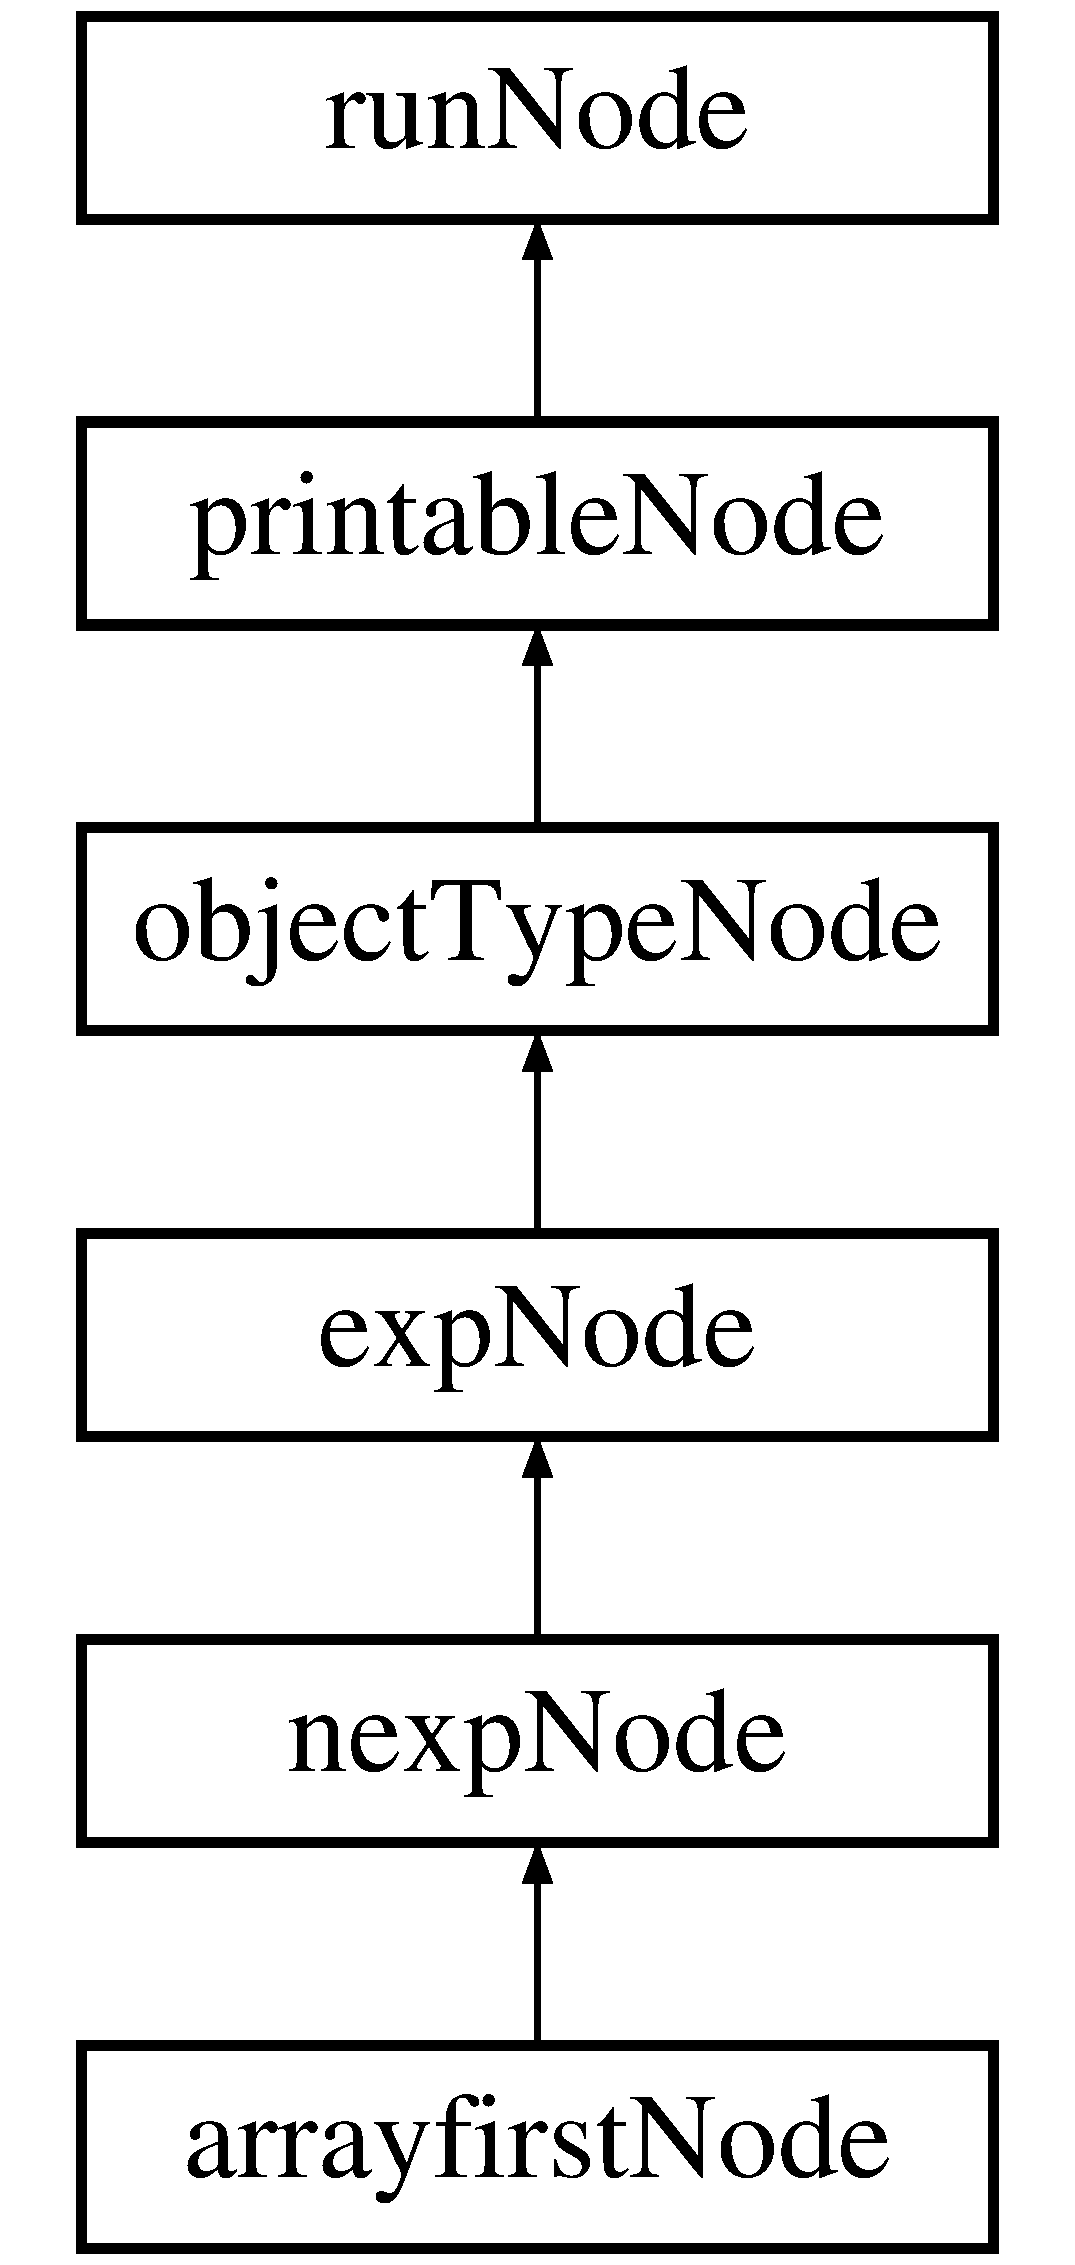
\includegraphics[height=6.000000cm]{classarrayfirstNode}
\end{center}
\end{figure}
\subsection*{Métodos públicos}
\begin{DoxyCompactItemize}
\item 
\hyperlink{classarrayfirstNode_a90ce782fc1cc3514e6f12839d3ceccea}{arrayfirst\-Node} (\hyperlink{classrunNode}{run\-Node} $\ast$array)
\item 
void \hyperlink{classarrayfirstNode_a6966767db3660da890d9d3c7363f8e90}{run} ()
\end{DoxyCompactItemize}
\subsection*{Métodos públicos estáticos}
\begin{DoxyCompactItemize}
\item 
static \hyperlink{classrunNode}{run\-Node} $\ast$ \hyperlink{classarrayfirstNode_aa94b0227fcfd30303ed314921ce83cbc}{as\-Method} ()
\end{DoxyCompactItemize}


\subsection{Descripción detallada}
Nodo función priemer elemento de array. 

Este nodo se utiliza para obtener el primer elemento de un array, o un nodo nulo si este está vacío. 

\subsection{Documentación del constructor y destructor}
\hypertarget{classarrayfirstNode_a90ce782fc1cc3514e6f12839d3ceccea}{\index{arrayfirst\-Node@{arrayfirst\-Node}!arrayfirst\-Node@{arrayfirst\-Node}}
\index{arrayfirst\-Node@{arrayfirst\-Node}!arrayfirstNode@{arrayfirst\-Node}}
\subsubsection[{arrayfirst\-Node}]{\setlength{\rightskip}{0pt plus 5cm}arrayfirst\-Node\-::arrayfirst\-Node (
\begin{DoxyParamCaption}
\item[{{\bf run\-Node} $\ast$}]{array}
\end{DoxyParamCaption}
)}}\label{classarrayfirstNode_a90ce782fc1cc3514e6f12839d3ceccea}
Constructor de la clase 
\begin{DoxyParams}{Parámetros}
{\em array} & Nodo que representa el array \\
\hline
\end{DoxyParams}


\subsection{Documentación de las funciones miembro}
\hypertarget{classarrayfirstNode_aa94b0227fcfd30303ed314921ce83cbc}{\index{arrayfirst\-Node@{arrayfirst\-Node}!as\-Method@{as\-Method}}
\index{as\-Method@{as\-Method}!arrayfirstNode@{arrayfirst\-Node}}
\subsubsection[{as\-Method}]{\setlength{\rightskip}{0pt plus 5cm}{\bf run\-Node} $\ast$ arrayfirst\-Node\-::as\-Method (
\begin{DoxyParamCaption}
{}
\end{DoxyParamCaption}
)\hspace{0.3cm}{\ttfamily [static]}}}\label{classarrayfirstNode_aa94b0227fcfd30303ed314921ce83cbc}
Devuelve un nodo primer elemento de array como cuerpo de un nodo función, siendo un nodo this el array de elementos. \begin{DoxyReturn}{Devuelve}
Método first. 
\end{DoxyReturn}
\hypertarget{classarrayfirstNode_a6966767db3660da890d9d3c7363f8e90}{\index{arrayfirst\-Node@{arrayfirst\-Node}!run@{run}}
\index{run@{run}!arrayfirstNode@{arrayfirst\-Node}}
\subsubsection[{run}]{\setlength{\rightskip}{0pt plus 5cm}void arrayfirst\-Node\-::run (
\begin{DoxyParamCaption}
{}
\end{DoxyParamCaption}
)\hspace{0.3cm}{\ttfamily [virtual]}}}\label{classarrayfirstNode_a6966767db3660da890d9d3c7363f8e90}
Método que ejecuta el nodo. Toma como valor una referencia al primer elemento de un array, o a un nodo nulo si el array está vacío. 

Implementa \hyperlink{classrunNode_a83c10df8148829b08e04153c93d69eec}{run\-Node}.



La documentación para esta clase fue generada a partir de los siguientes ficheros\-:\begin{DoxyCompactItemize}
\item 
trunk/src/run/operators/\hyperlink{arrayOpNode_8h}{array\-Op\-Node.\-h}\item 
trunk/src/run/operators/array\-Op\-Node.\-cpp\end{DoxyCompactItemize}

\hypertarget{classarrayinsertNode}{\section{Referencia de la Clase arrayinsert\-Node}
\label{classarrayinsertNode}\index{arrayinsert\-Node@{arrayinsert\-Node}}
}


Nodo función insertar elemento en array.  




{\ttfamily \#include $<$array\-Op\-Node.\-h$>$}

Diagrama de herencias de arrayinsert\-Node\begin{figure}[H]
\begin{center}
\leavevmode
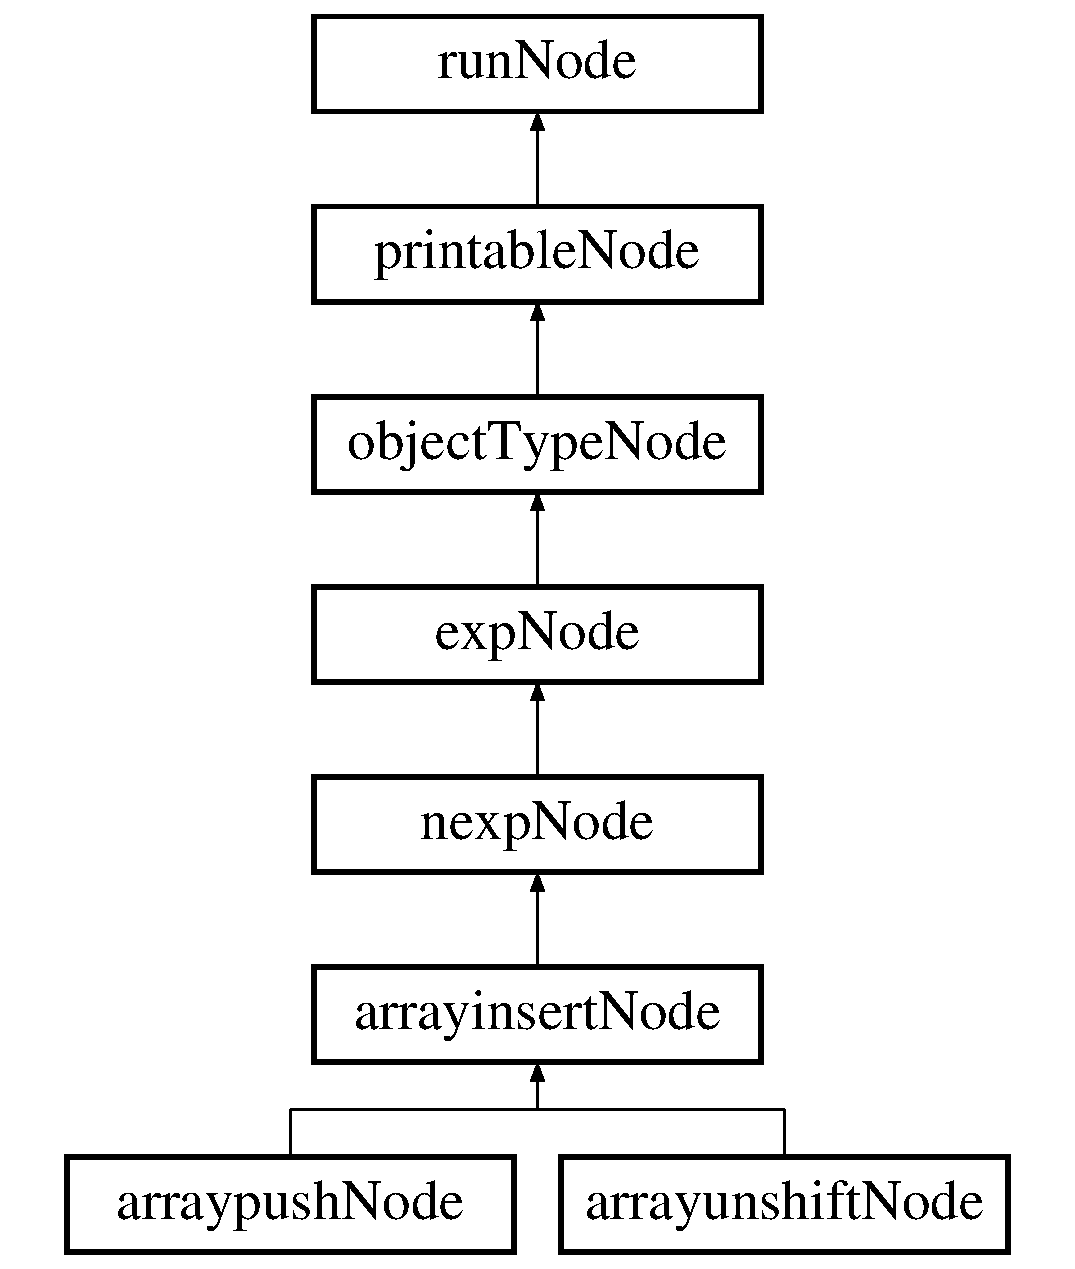
\includegraphics[height=7.000000cm]{classarrayinsertNode}
\end{center}
\end{figure}
\subsection*{Métodos públicos}
\begin{DoxyCompactItemize}
\item 
\hyperlink{classarrayinsertNode_a018b6d84b64e515eea1016810ed335ac}{arrayinsert\-Node} (\hyperlink{classrunNode}{run\-Node} $\ast$array, \hyperlink{classrunNode}{run\-Node} $\ast$index, \hyperlink{classrunNode}{run\-Node} $\ast$element)
\item 
void \hyperlink{classarrayinsertNode_a1a72ddaf1ade1ee8a535ae1ca1fc2861}{run} ()
\end{DoxyCompactItemize}
\subsection*{Métodos públicos estáticos}
\begin{DoxyCompactItemize}
\item 
static \hyperlink{classrunNode}{run\-Node} $\ast$ \hyperlink{classarrayinsertNode_ab9edbaa7c002c24e3bedf5d2bd8ca5be}{as\-Method} ()
\end{DoxyCompactItemize}


\subsection{Descripción detallada}
Nodo función insertar elemento en array. 

Se encarga de insertar un eleemtno en una posición dada de un array. Si la posición se encuentra fuera de rango se produce un error. 

\subsection{Documentación del constructor y destructor}
\hypertarget{classarrayinsertNode_a018b6d84b64e515eea1016810ed335ac}{\index{arrayinsert\-Node@{arrayinsert\-Node}!arrayinsert\-Node@{arrayinsert\-Node}}
\index{arrayinsert\-Node@{arrayinsert\-Node}!arrayinsertNode@{arrayinsert\-Node}}
\subsubsection[{arrayinsert\-Node}]{\setlength{\rightskip}{0pt plus 5cm}arrayinsert\-Node\-::arrayinsert\-Node (
\begin{DoxyParamCaption}
\item[{{\bf run\-Node} $\ast$}]{array, }
\item[{{\bf run\-Node} $\ast$}]{index, }
\item[{{\bf run\-Node} $\ast$}]{element}
\end{DoxyParamCaption}
)}}\label{classarrayinsertNode_a018b6d84b64e515eea1016810ed335ac}
Constructor de la clase 
\begin{DoxyParams}{Parámetros}
{\em array} & Nodo que representa el array \\
\hline
{\em index} & Nodo que representa la posicion en la que se llevará a cabo la inserción \\
\hline
{\em element} & Nodo que representa el elemento que será insertado \\
\hline
\end{DoxyParams}


\subsection{Documentación de las funciones miembro}
\hypertarget{classarrayinsertNode_ab9edbaa7c002c24e3bedf5d2bd8ca5be}{\index{arrayinsert\-Node@{arrayinsert\-Node}!as\-Method@{as\-Method}}
\index{as\-Method@{as\-Method}!arrayinsertNode@{arrayinsert\-Node}}
\subsubsection[{as\-Method}]{\setlength{\rightskip}{0pt plus 5cm}{\bf run\-Node} $\ast$ arrayinsert\-Node\-::as\-Method (
\begin{DoxyParamCaption}
{}
\end{DoxyParamCaption}
)\hspace{0.3cm}{\ttfamily [static]}}}\label{classarrayinsertNode_ab9edbaa7c002c24e3bedf5d2bd8ca5be}
Devuelve un nodo insertar elemento en array como cuerpo de un nodo función, siendo un nodo this el array de elementos. \begin{DoxyReturn}{Devuelve}
Método insert. 
\end{DoxyReturn}
\hypertarget{classarrayinsertNode_a1a72ddaf1ade1ee8a535ae1ca1fc2861}{\index{arrayinsert\-Node@{arrayinsert\-Node}!run@{run}}
\index{run@{run}!arrayinsertNode@{arrayinsert\-Node}}
\subsubsection[{run}]{\setlength{\rightskip}{0pt plus 5cm}void arrayinsert\-Node\-::run (
\begin{DoxyParamCaption}
{}
\end{DoxyParamCaption}
)\hspace{0.3cm}{\ttfamily [virtual]}}}\label{classarrayinsertNode_a1a72ddaf1ade1ee8a535ae1ca1fc2861}
Método que lleva a cabo la ejecución del nodo. Inserta el elemento en la posicón dada y toma como valor una referencia al array con el elemento insertado 

Implementa \hyperlink{classrunNode_a83c10df8148829b08e04153c93d69eec}{run\-Node}.



Reimplementado en \hyperlink{classarraypushNode_a6eb706763d3f8cc7715706005d4bf049}{arraypush\-Node}.



La documentación para esta clase fue generada a partir de los siguientes ficheros\-:\begin{DoxyCompactItemize}
\item 
trunk/src/run/operators/\hyperlink{arrayOpNode_8h}{array\-Op\-Node.\-h}\item 
trunk/src/run/operators/array\-Op\-Node.\-cpp\end{DoxyCompactItemize}

\hypertarget{classarraylastNode}{\section{Referencia de la Clase arraylast\-Node}
\label{classarraylastNode}\index{arraylast\-Node@{arraylast\-Node}}
}


Nodo obtener último elemento de array.  




{\ttfamily \#include $<$array\-Op\-Node.\-h$>$}

Diagrama de herencias de arraylast\-Node\begin{figure}[H]
\begin{center}
\leavevmode
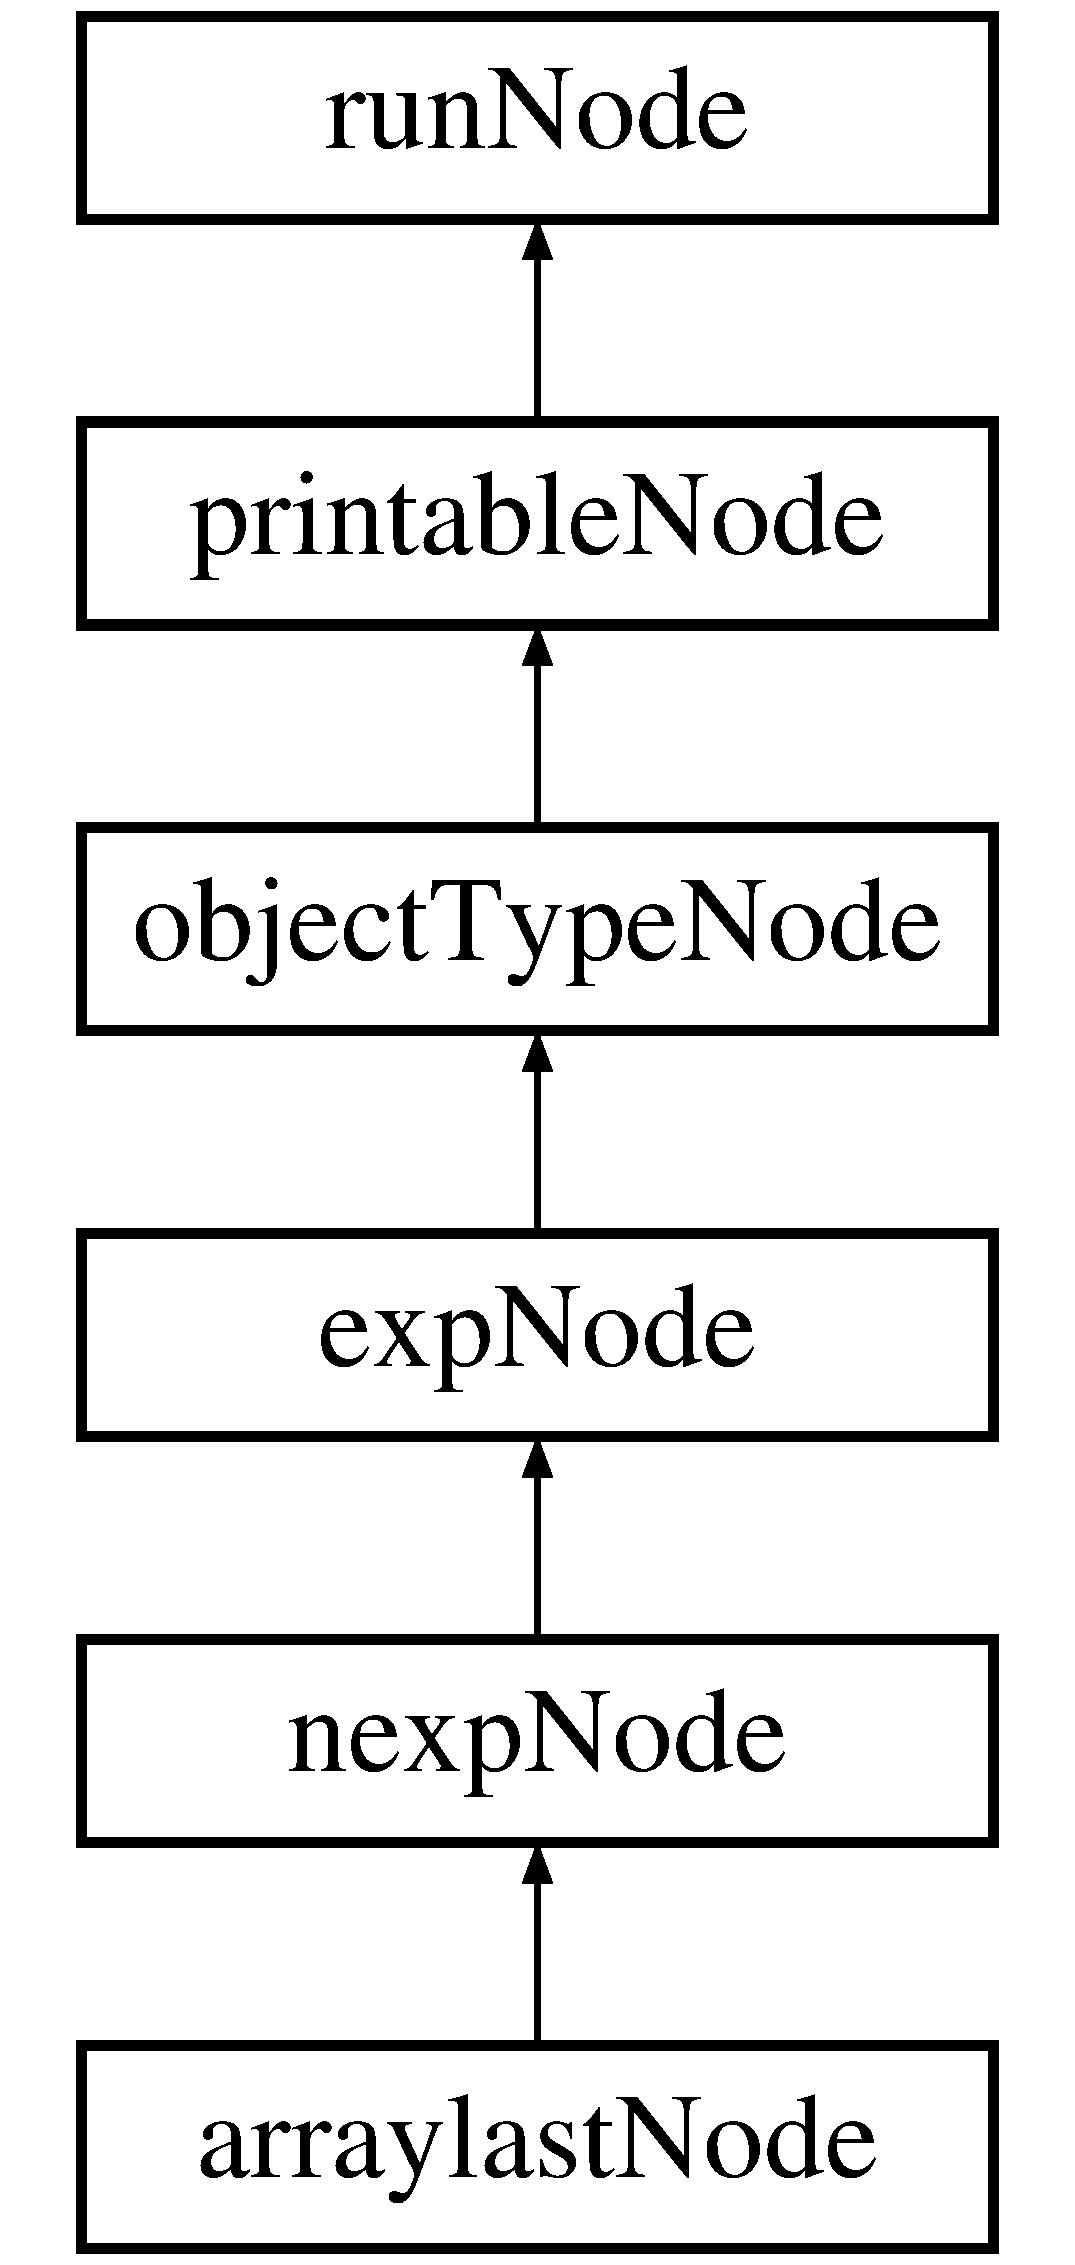
\includegraphics[height=6.000000cm]{classarraylastNode}
\end{center}
\end{figure}
\subsection*{Métodos públicos}
\begin{DoxyCompactItemize}
\item 
\hyperlink{classarraylastNode_a17f8b2bbc08ddfd7d5cb082ef036d94c}{arraylast\-Node} (\hyperlink{classrunNode}{run\-Node} $\ast$array)
\item 
void \hyperlink{classarraylastNode_a408528a55b63a926c665dac74764319a}{run} ()
\end{DoxyCompactItemize}
\subsection*{Métodos públicos estáticos}
\begin{DoxyCompactItemize}
\item 
static \hyperlink{classrunNode}{run\-Node} $\ast$ \hyperlink{classarraylastNode_a0506ee0202021a4ddc48aaf5be139927}{as\-Method} ()
\end{DoxyCompactItemize}


\subsection{Descripción detallada}
Nodo obtener último elemento de array. 

Este nodo se utiliza para obtener el último elemento de un array, o un nodo nulo si este está vacío. 

\subsection{Documentación del constructor y destructor}
\hypertarget{classarraylastNode_a17f8b2bbc08ddfd7d5cb082ef036d94c}{\index{arraylast\-Node@{arraylast\-Node}!arraylast\-Node@{arraylast\-Node}}
\index{arraylast\-Node@{arraylast\-Node}!arraylastNode@{arraylast\-Node}}
\subsubsection[{arraylast\-Node}]{\setlength{\rightskip}{0pt plus 5cm}arraylast\-Node\-::arraylast\-Node (
\begin{DoxyParamCaption}
\item[{{\bf run\-Node} $\ast$}]{array}
\end{DoxyParamCaption}
)}}\label{classarraylastNode_a17f8b2bbc08ddfd7d5cb082ef036d94c}
Constructor de la clase 
\begin{DoxyParams}{Parámetros}
{\em array} & Nodo que representa el array \\
\hline
\end{DoxyParams}


\subsection{Documentación de las funciones miembro}
\hypertarget{classarraylastNode_a0506ee0202021a4ddc48aaf5be139927}{\index{arraylast\-Node@{arraylast\-Node}!as\-Method@{as\-Method}}
\index{as\-Method@{as\-Method}!arraylastNode@{arraylast\-Node}}
\subsubsection[{as\-Method}]{\setlength{\rightskip}{0pt plus 5cm}{\bf run\-Node} $\ast$ arraylast\-Node\-::as\-Method (
\begin{DoxyParamCaption}
{}
\end{DoxyParamCaption}
)\hspace{0.3cm}{\ttfamily [static]}}}\label{classarraylastNode_a0506ee0202021a4ddc48aaf5be139927}
Devuelve un nodo último elemento de array como cuerpo de un nodo función, siendo un nodo this el array de elementos. \begin{DoxyReturn}{Devuelve}
Método last. 
\end{DoxyReturn}
\hypertarget{classarraylastNode_a408528a55b63a926c665dac74764319a}{\index{arraylast\-Node@{arraylast\-Node}!run@{run}}
\index{run@{run}!arraylastNode@{arraylast\-Node}}
\subsubsection[{run}]{\setlength{\rightskip}{0pt plus 5cm}void arraylast\-Node\-::run (
\begin{DoxyParamCaption}
{}
\end{DoxyParamCaption}
)\hspace{0.3cm}{\ttfamily [virtual]}}}\label{classarraylastNode_a408528a55b63a926c665dac74764319a}
Método que ejecuta el nodo. Toma como valor una referencia al último elemento de un array, o a un nodo nulo si el array está vacío. 

Implementa \hyperlink{classrunNode_a83c10df8148829b08e04153c93d69eec}{run\-Node}.



La documentación para esta clase fue generada a partir de los siguientes ficheros\-:\begin{DoxyCompactItemize}
\item 
trunk/src/run/operators/\hyperlink{arrayOpNode_8h}{array\-Op\-Node.\-h}\item 
trunk/src/run/operators/array\-Op\-Node.\-cpp\end{DoxyCompactItemize}

\hypertarget{classarrayNode}{\section{Referencia de la Clase array\-Node}
\label{classarrayNode}\index{array\-Node@{array\-Node}}
}


Nodo array.  




{\ttfamily \#include $<$type\-Node.\-h$>$}

Diagrama de herencias de array\-Node\begin{figure}[H]
\begin{center}
\leavevmode
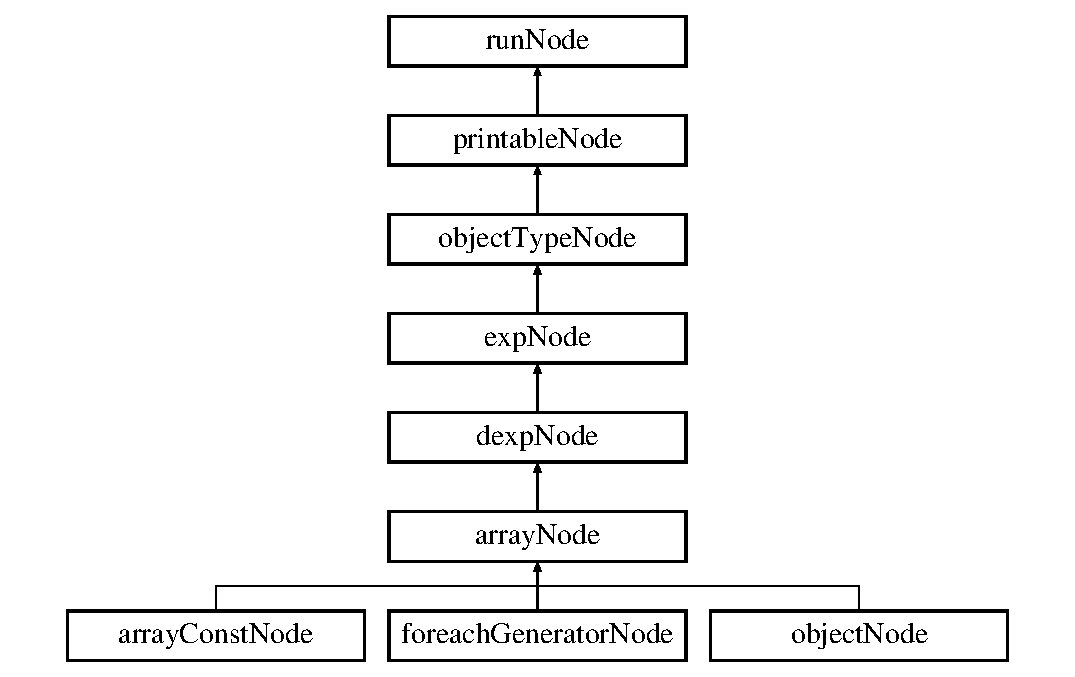
\includegraphics[height=7.000000cm]{classarrayNode}
\end{center}
\end{figure}
\subsection*{Métodos públicos}
\begin{DoxyCompactItemize}
\item 
\hyperlink{classarrayNode_aec5963f3935e85c4a08705ec96ee4a4e}{array\-Node} (\hyperlink{classlistNode}{list\-Node} $\ast$list)
\item 
\hyperlink{classarrayNode_a088c20eb41de79e7f787e8a965e1f3f1}{array\-Node} ()
\item 
\hyperlink{classarrayNode_aecbe93c9bc3651585e1cf8951cae40ed}{array\-Node} (\hyperlink{classarrayNode}{array\-Node} $\ast$array)
\item 
\hyperlink{classarrayNode_afbaaec4d754c215fbb8513170d0e282a}{array\-Node} (\hyperlink{classarrayNode}{array\-Node} $\ast$array, \hyperlink{classrefNode}{ref\-Node} $\ast$\&ref\-Search)
\item 
void \hyperlink{classarrayNode_a5ead9863a0f9478798c7777a0c03b1a5}{run} ()
\item 
string \hyperlink{classarrayNode_a7d68669075eec824abc4400f18670075}{print} () const 
\item 
\hyperlink{classsymbolsTable}{symbols} $\ast$ \hyperlink{classarrayNode_a95eea3900dfa813fba8f25dba0f8456c}{get\-Array} ()
\item 
void \hyperlink{classarrayNode_a2ccdc9126f6e778d5623b4e3a6539d19}{insert} (\hyperlink{classrunNode}{run\-Node} $\ast$key, \hyperlink{classrunNode}{run\-Node} $\ast$val, bool str=false)
\item 
void \hyperlink{classarrayNode_a15ff4fc8cc43321084be7c38f9e9ae43}{del} (\hyperlink{classrunNode}{run\-Node} $\ast$key, bool str=false, bool force\-\_\-position=false)
\item 
\hyperlink{classrunNode}{run\-Node} $\ast$ \hyperlink{classarrayNode_ac45e2ad7a922801ac99e4650d2351c96}{get} (\hyperlink{classrunNode}{run\-Node} $\ast$key, bool str=false)
\item 
int \hyperlink{classarrayNode_a0fc0d195f693f8ec2884726eec7211cf}{size} () const 
\item 
bool \hyperlink{classarrayNode_a7d5003af8f4e70e65c5b8ca7cdd5a842}{compare} (\hyperlink{classrunNode}{run\-Node} $\ast$node, int op=0)
\item 
int \hyperlink{classarrayNode_a507607cad03ce0c2d0e1de5f80b71362}{get\-Count} () const 
\item 
void \hyperlink{classarrayNode_a38fced3677c6aced8b37cc9510711970}{c\-All} (\hyperlink{classrunNode}{run\-Node} $\ast$node\-\_\-search, \hyperlink{classrunNode}{run\-Node} $\ast$node\-\_\-new)
\item 
bool \hyperlink{classarrayNode_a9e58c867215bef0ab3dfd4db78d6b2f2}{isref} (\hyperlink{classrunNode}{run\-Node} $\ast$node)
\item 
void \hyperlink{classarrayNode_a8e37cc53c47cf7c264757e25d50af586}{clear} ()
\item 
void \hyperlink{classarrayNode_a907ba507d3fa9e402499dfb13cfec835}{clear\-Ref} ()
\item 
void \hyperlink{classarrayNode_ac478825dc6f392ed96fc81cbc61758ca}{set\-Array} (\hyperlink{classsymbolsTable}{symbols} array)
\item 
void \hyperlink{classarrayNode_a88cd3c520d82d253fee5d7b5f5c857f9}{push} (\hyperlink{classrunNode}{run\-Node} $\ast$node)
\item 
virtual \hyperlink{classrunNode}{run\-Node} $\ast$ \hyperlink{classarrayNode_aa2a23e8d7e23dfc039ecdd17badf2324}{copy\-Array} (\hyperlink{classarrayNode}{array\-Node} $\ast$a)
\item 
\hyperlink{classrunNode}{run\-Node} $\ast$ \hyperlink{classarrayNode_adb8aba7525e34c7aec375f58be182bd8}{get\-Class} ()
\item 
bool \hyperlink{classarrayNode_af18a8d4f5e369713a01387bad022db72}{boolvalue} () const 
\item 
num \hyperlink{classarrayNode_a8a862493dfcab500edd9acf4f4c55348}{numvalue} () const 
\item 
string \hyperlink{classarrayNode_a3e5771d0cf67476bfe19683d504327d1}{strvalue} () const 
\item 
\hyperlink{classarrayNode_a9076d616c925d5b6dfee1164279f3763}{$\sim$array\-Node} ()
\end{DoxyCompactItemize}
\subsection*{Métodos públicos estáticos}
\begin{DoxyCompactItemize}
\item 
static void \hyperlink{classarrayNode_a4e87dab3b6a894b583aa47199bf64741}{generate\-Class} ()
\end{DoxyCompactItemize}
\subsection*{Métodos protegidos}
\begin{DoxyCompactItemize}
\item 
string \hyperlink{classarrayNode_aedc687b42ca8accbc226bce834a7a7d5}{print\-Level} (short int level) const 
\end{DoxyCompactItemize}


\subsection{Descripción detallada}
Nodo array. 

Representa un vector de elementos. Los array son nodos que presenta una tabla de símbolos interna en la que almacena referencias a cada uno de los elementos en el array.

En la inicialización del árbol de ejecución el nodo array se asocia con una lista de nodos de listas (\hyperlink{classlistNode}{list\-Node}).

En la ejecución del nodo array los valores de la lista son guardados en la tabla de símbolos del array. En el caso de que los valores sean nodos asociativos (\begin{DoxySeeAlso}{Ver también}
\hyperlink{classmapNode}{map\-Node}) se establece la clave como referencia. En caso contrario se utiliza como referencia un entero correspondiente a la posición \hyperlink{classarrayNode_a15ff4fc8cc43321084be7c38f9e9ae43}{del} elemento en la lista.
\end{DoxySeeAlso}
Todo nodo array tiene asociado un nodo clase \char`\"{}array\-Class\char`\"{}. 

\subsection{Documentación del constructor y destructor}
\hypertarget{classarrayNode_aec5963f3935e85c4a08705ec96ee4a4e}{\index{array\-Node@{array\-Node}!array\-Node@{array\-Node}}
\index{array\-Node@{array\-Node}!arrayNode@{array\-Node}}
\subsubsection[{array\-Node}]{\setlength{\rightskip}{0pt plus 5cm}array\-Node\-::array\-Node (
\begin{DoxyParamCaption}
\item[{{\bf list\-Node} $\ast$}]{list}
\end{DoxyParamCaption}
)}}\label{classarrayNode_aec5963f3935e85c4a08705ec96ee4a4e}
Constructor de clase. 
\begin{DoxyParams}{Parámetros}
{\em list} & Nodo lista. \\
\hline
\end{DoxyParams}
\hypertarget{classarrayNode_a088c20eb41de79e7f787e8a965e1f3f1}{\index{array\-Node@{array\-Node}!array\-Node@{array\-Node}}
\index{array\-Node@{array\-Node}!arrayNode@{array\-Node}}
\subsubsection[{array\-Node}]{\setlength{\rightskip}{0pt plus 5cm}array\-Node\-::array\-Node (
\begin{DoxyParamCaption}
{}
\end{DoxyParamCaption}
)}}\label{classarrayNode_a088c20eb41de79e7f787e8a965e1f3f1}
Constructor de array vacío. \hypertarget{classarrayNode_aecbe93c9bc3651585e1cf8951cae40ed}{\index{array\-Node@{array\-Node}!array\-Node@{array\-Node}}
\index{array\-Node@{array\-Node}!arrayNode@{array\-Node}}
\subsubsection[{array\-Node}]{\setlength{\rightskip}{0pt plus 5cm}array\-Node\-::array\-Node (
\begin{DoxyParamCaption}
\item[{{\bf array\-Node} $\ast$}]{array}
\end{DoxyParamCaption}
)}}\label{classarrayNode_aecbe93c9bc3651585e1cf8951cae40ed}
Constructor copia. 
\begin{DoxyParams}{Parámetros}
{\em array} & Nodo array para la copia. \\
\hline
\end{DoxyParams}
\hypertarget{classarrayNode_afbaaec4d754c215fbb8513170d0e282a}{\index{array\-Node@{array\-Node}!array\-Node@{array\-Node}}
\index{array\-Node@{array\-Node}!arrayNode@{array\-Node}}
\subsubsection[{array\-Node}]{\setlength{\rightskip}{0pt plus 5cm}array\-Node\-::array\-Node (
\begin{DoxyParamCaption}
\item[{{\bf array\-Node} $\ast$}]{array, }
\item[{{\bf ref\-Node} $\ast$\&}]{ref\-Search}
\end{DoxyParamCaption}
)}}\label{classarrayNode_afbaaec4d754c215fbb8513170d0e282a}
Constructor copia. Durante la creación del objeto busca una referencia en el nodo copiado que toma el valor de la nueva referencia en el nodo. 
\begin{DoxyParams}{Parámetros}
{\em array} & Nodo array para la copia. \\
\hline
{\em ref\-Search} & Valor que será buscado. \\
\hline
\end{DoxyParams}
\hypertarget{classarrayNode_a9076d616c925d5b6dfee1164279f3763}{\index{array\-Node@{array\-Node}!$\sim$array\-Node@{$\sim$array\-Node}}
\index{$\sim$array\-Node@{$\sim$array\-Node}!arrayNode@{array\-Node}}
\subsubsection[{$\sim$array\-Node}]{\setlength{\rightskip}{0pt plus 5cm}array\-Node\-::$\sim$array\-Node (
\begin{DoxyParamCaption}
{}
\end{DoxyParamCaption}
)}}\label{classarrayNode_a9076d616c925d5b6dfee1164279f3763}
Método destructor del array. El cual consiste en la eliminación de los elementos en la tabla de símbolos. 

\subsection{Documentación de las funciones miembro}
\hypertarget{classarrayNode_af18a8d4f5e369713a01387bad022db72}{\index{array\-Node@{array\-Node}!boolvalue@{boolvalue}}
\index{boolvalue@{boolvalue}!arrayNode@{array\-Node}}
\subsubsection[{boolvalue}]{\setlength{\rightskip}{0pt plus 5cm}bool array\-Node\-::boolvalue (
\begin{DoxyParamCaption}
{}
\end{DoxyParamCaption}
) const\hspace{0.3cm}{\ttfamily [virtual]}}}\label{classarrayNode_af18a8d4f5e369713a01387bad022db72}
Obtiene el valor booleano del array. El cual indica si este es vacío. \begin{DoxyReturn}{Devuelve}
Valor booleano del array. 
\end{DoxyReturn}


Reimplementado de \hyperlink{classdexpNode_a18781e07cc3390c04b6905249755ccc8}{dexp\-Node}.

\hypertarget{classarrayNode_a38fced3677c6aced8b37cc9510711970}{\index{array\-Node@{array\-Node}!c\-All@{c\-All}}
\index{c\-All@{c\-All}!arrayNode@{array\-Node}}
\subsubsection[{c\-All}]{\setlength{\rightskip}{0pt plus 5cm}void array\-Node\-::c\-All (
\begin{DoxyParamCaption}
\item[{{\bf run\-Node} $\ast$}]{node\-\_\-search, }
\item[{{\bf run\-Node} $\ast$}]{node\-\_\-new}
\end{DoxyParamCaption}
)}}\label{classarrayNode_a38fced3677c6aced8b37cc9510711970}
Busca en los elementos del array toda referencia al nodo node\-\_\-search y la cambia por una referencia a node\-\_\-new.

Si algún elemento es otro array se busca de igual forma en el mismo.


\begin{DoxyParams}{Parámetros}
{\em node\-\_\-search} & Nodo a buscar. \\
\hline
{\em node\-\_\-new} & Nodo nuevo. \\
\hline
\end{DoxyParams}
\hypertarget{classarrayNode_a8e37cc53c47cf7c264757e25d50af586}{\index{array\-Node@{array\-Node}!clear@{clear}}
\index{clear@{clear}!arrayNode@{array\-Node}}
\subsubsection[{clear}]{\setlength{\rightskip}{0pt plus 5cm}void array\-Node\-::clear (
\begin{DoxyParamCaption}
{}
\end{DoxyParamCaption}
)}}\label{classarrayNode_a8e37cc53c47cf7c264757e25d50af586}
Elimina todos los elementos del array. \hypertarget{classarrayNode_a907ba507d3fa9e402499dfb13cfec835}{\index{array\-Node@{array\-Node}!clear\-Ref@{clear\-Ref}}
\index{clear\-Ref@{clear\-Ref}!arrayNode@{array\-Node}}
\subsubsection[{clear\-Ref}]{\setlength{\rightskip}{0pt plus 5cm}void array\-Node\-::clear\-Ref (
\begin{DoxyParamCaption}
{}
\end{DoxyParamCaption}
)}}\label{classarrayNode_a907ba507d3fa9e402499dfb13cfec835}
Elimina únicamente las referencias en el array. \hypertarget{classarrayNode_a7d5003af8f4e70e65c5b8ca7cdd5a842}{\index{array\-Node@{array\-Node}!compare@{compare}}
\index{compare@{compare}!arrayNode@{array\-Node}}
\subsubsection[{compare}]{\setlength{\rightskip}{0pt plus 5cm}bool array\-Node\-::compare (
\begin{DoxyParamCaption}
\item[{{\bf run\-Node} $\ast$}]{node, }
\item[{int}]{op = {\ttfamily 0}}
\end{DoxyParamCaption}
)}}\label{classarrayNode_a7d5003af8f4e70e65c5b8ca7cdd5a842}
Compara elemento a elemento el nodo array con el nodo pasado como parámetro.


\begin{DoxyParams}{Parámetros}
{\em node} & Nodo a comparar. \\
\hline
{\em op.} & Operador a aplicar case 0\-: == case 1\-: != case 2\-: $>$ case 3\-: $<$ case 4\-: $>$= case 5\-: $<$= case 6\-: === \\
\hline
\end{DoxyParams}
\begin{DoxyReturn}{Devuelve}
Booleano resultado de la operación. 
\end{DoxyReturn}
\hypertarget{classarrayNode_aa2a23e8d7e23dfc039ecdd17badf2324}{\index{array\-Node@{array\-Node}!copy\-Array@{copy\-Array}}
\index{copy\-Array@{copy\-Array}!arrayNode@{array\-Node}}
\subsubsection[{copy\-Array}]{\setlength{\rightskip}{0pt plus 5cm}{\bf run\-Node} $\ast$ array\-Node\-::copy\-Array (
\begin{DoxyParamCaption}
\item[{{\bf array\-Node} $\ast$}]{a}
\end{DoxyParamCaption}
)\hspace{0.3cm}{\ttfamily [virtual]}}}\label{classarrayNode_aa2a23e8d7e23dfc039ecdd17badf2324}
Copia el contenido de un array en otro nuevo. 
\begin{DoxyParams}{Parámetros}
{\em a} & Array a copiar. \\
\hline
\end{DoxyParams}
\begin{DoxyReturn}{Devuelve}
Array resultado de la copia. 
\end{DoxyReturn}
\hypertarget{classarrayNode_a15ff4fc8cc43321084be7c38f9e9ae43}{\index{array\-Node@{array\-Node}!del@{del}}
\index{del@{del}!arrayNode@{array\-Node}}
\subsubsection[{del}]{\setlength{\rightskip}{0pt plus 5cm}void array\-Node\-::del (
\begin{DoxyParamCaption}
\item[{{\bf run\-Node} $\ast$}]{key, }
\item[{bool}]{str = {\ttfamily false}, }
\item[{bool}]{force\-\_\-position = {\ttfamily false}}
\end{DoxyParamCaption}
)}}\label{classarrayNode_a15ff4fc8cc43321084be7c38f9e9ae43}
Elimina un elemento del array. 
\begin{DoxyParams}{Parámetros}
{\em key} & Nodo clave. \\
\hline
{\em str} & Determina si las clave será forzada a tomarse como cadena. \\
\hline
{\em force\-\_\-position} & Fuerza a que la clave sea tomada como posición numérica. \\
\hline
\end{DoxyParams}
\hypertarget{classarrayNode_a4e87dab3b6a894b583aa47199bf64741}{\index{array\-Node@{array\-Node}!generate\-Class@{generate\-Class}}
\index{generate\-Class@{generate\-Class}!arrayNode@{array\-Node}}
\subsubsection[{generate\-Class}]{\setlength{\rightskip}{0pt plus 5cm}void array\-Node\-::generate\-Class (
\begin{DoxyParamCaption}
{}
\end{DoxyParamCaption}
)\hspace{0.3cm}{\ttfamily [static]}}}\label{classarrayNode_a4e87dab3b6a894b583aa47199bf64741}
Genera la clase \char`\"{}array\-Class\char`\"{} asociada a todo array. \hypertarget{classarrayNode_ac45e2ad7a922801ac99e4650d2351c96}{\index{array\-Node@{array\-Node}!get@{get}}
\index{get@{get}!arrayNode@{array\-Node}}
\subsubsection[{get}]{\setlength{\rightskip}{0pt plus 5cm}{\bf run\-Node} $\ast$ array\-Node\-::get (
\begin{DoxyParamCaption}
\item[{{\bf run\-Node} $\ast$}]{key, }
\item[{bool}]{str = {\ttfamily false}}
\end{DoxyParamCaption}
)}}\label{classarrayNode_ac45e2ad7a922801ac99e4650d2351c96}
Obtiene un elemento a partir de una clave. 
\begin{DoxyParams}{Parámetros}
{\em key} & Nodo clave. \\
\hline
{\em str} & Determina si las clave será forzada a tomarse como cadena. \\
\hline
\end{DoxyParams}
\begin{DoxyReturn}{Devuelve}
Nodo correspondiente a la clave. N\-U\-L\-L si no existe. 
\end{DoxyReturn}
\hypertarget{classarrayNode_a95eea3900dfa813fba8f25dba0f8456c}{\index{array\-Node@{array\-Node}!get\-Array@{get\-Array}}
\index{get\-Array@{get\-Array}!arrayNode@{array\-Node}}
\subsubsection[{get\-Array}]{\setlength{\rightskip}{0pt plus 5cm}{\bf symbols} $\ast$ array\-Node\-::get\-Array (
\begin{DoxyParamCaption}
{}
\end{DoxyParamCaption}
)}}\label{classarrayNode_a95eea3900dfa813fba8f25dba0f8456c}
Obtiene la tabla de símbolos interna del nodo. 
\begin{DoxyParams}{Parámetros}
{\em Tabla} & de símbolos interna. \\
\hline
\end{DoxyParams}
\hypertarget{classarrayNode_adb8aba7525e34c7aec375f58be182bd8}{\index{array\-Node@{array\-Node}!get\-Class@{get\-Class}}
\index{get\-Class@{get\-Class}!arrayNode@{array\-Node}}
\subsubsection[{get\-Class}]{\setlength{\rightskip}{0pt plus 5cm}{\bf run\-Node} $\ast$ array\-Node\-::get\-Class (
\begin{DoxyParamCaption}
{}
\end{DoxyParamCaption}
)\hspace{0.3cm}{\ttfamily [virtual]}}}\label{classarrayNode_adb8aba7525e34c7aec375f58be182bd8}
Obtiene el nodo clase asociado a la clase. \begin{DoxyReturn}{Devuelve}
Nodo clase. 
\end{DoxyReturn}


Reimplementado de \hyperlink{classobjectTypeNode_a42d4efaea6b650ef72807de94d3baa37}{object\-Type\-Node}.



Reimplementado en \hyperlink{classobjectNode_a09303f23cd355cf6c404db07f0b4428c}{object\-Node}.

\hypertarget{classarrayNode_a507607cad03ce0c2d0e1de5f80b71362}{\index{array\-Node@{array\-Node}!get\-Count@{get\-Count}}
\index{get\-Count@{get\-Count}!arrayNode@{array\-Node}}
\subsubsection[{get\-Count}]{\setlength{\rightskip}{0pt plus 5cm}int array\-Node\-::get\-Count (
\begin{DoxyParamCaption}
{}
\end{DoxyParamCaption}
) const}}\label{classarrayNode_a507607cad03ce0c2d0e1de5f80b71362}
Obtiene el índice numérico actual. \begin{DoxyReturn}{Devuelve}
Numérico que indica el índice mayor. 
\end{DoxyReturn}
\hypertarget{classarrayNode_a2ccdc9126f6e778d5623b4e3a6539d19}{\index{array\-Node@{array\-Node}!insert@{insert}}
\index{insert@{insert}!arrayNode@{array\-Node}}
\subsubsection[{insert}]{\setlength{\rightskip}{0pt plus 5cm}void array\-Node\-::insert (
\begin{DoxyParamCaption}
\item[{{\bf run\-Node} $\ast$}]{key, }
\item[{{\bf run\-Node} $\ast$}]{val, }
\item[{bool}]{str = {\ttfamily false}}
\end{DoxyParamCaption}
)}}\label{classarrayNode_a2ccdc9126f6e778d5623b4e3a6539d19}
Inserta un elemento en el array. 
\begin{DoxyParams}{Parámetros}
{\em key} & Nodo clave del elemento. \\
\hline
{\em val} & Nodo valor del elemento. \\
\hline
{\em str} & Determina si las clave será forzada a tomarse como cadena. \\
\hline
\end{DoxyParams}
\hypertarget{classarrayNode_a9e58c867215bef0ab3dfd4db78d6b2f2}{\index{array\-Node@{array\-Node}!isref@{isref}}
\index{isref@{isref}!arrayNode@{array\-Node}}
\subsubsection[{isref}]{\setlength{\rightskip}{0pt plus 5cm}bool array\-Node\-::isref (
\begin{DoxyParamCaption}
\item[{{\bf run\-Node} $\ast$}]{node}
\end{DoxyParamCaption}
)}}\label{classarrayNode_a9e58c867215bef0ab3dfd4db78d6b2f2}
Dado un nodo ejecutable devuelve un booleano que indica si en el array se encuentra alguna referencia a dicho nodo.

Si algún elemento es otro array se busca de igual forma en el mismo.


\begin{DoxyParams}{Parámetros}
{\em node} & Nodo a buscar. \\
\hline
\end{DoxyParams}
\begin{DoxyReturn}{Devuelve}
Booleano que indica si el array mantiene alguna referencia. 
\end{DoxyReturn}
\hypertarget{classarrayNode_a8a862493dfcab500edd9acf4f4c55348}{\index{array\-Node@{array\-Node}!numvalue@{numvalue}}
\index{numvalue@{numvalue}!arrayNode@{array\-Node}}
\subsubsection[{numvalue}]{\setlength{\rightskip}{0pt plus 5cm}num array\-Node\-::numvalue (
\begin{DoxyParamCaption}
{}
\end{DoxyParamCaption}
) const\hspace{0.3cm}{\ttfamily [virtual]}}}\label{classarrayNode_a8a862493dfcab500edd9acf4f4c55348}
Obtiene el valor numérico del array el cual es 0. \begin{DoxyReturn}{Devuelve}
Valor numérico del array. 
\end{DoxyReturn}


Reimplementado de \hyperlink{classdexpNode_ae2d3bfed7e6ebd5e96ddcefaa230c3d2}{dexp\-Node}.

\hypertarget{classarrayNode_a7d68669075eec824abc4400f18670075}{\index{array\-Node@{array\-Node}!print@{print}}
\index{print@{print}!arrayNode@{array\-Node}}
\subsubsection[{print}]{\setlength{\rightskip}{0pt plus 5cm}string array\-Node\-::print (
\begin{DoxyParamCaption}
{}
\end{DoxyParamCaption}
) const\hspace{0.3cm}{\ttfamily [virtual]}}}\label{classarrayNode_a7d68669075eec824abc4400f18670075}
Determina cómo se imprime un nodo array. \begin{DoxyReturn}{Devuelve}
Valor cadena del array. 
\end{DoxyReturn}


Implementa \hyperlink{classprintableNode_ae5835e7b9d1a8af621723798137e01f9}{printable\-Node}.



Reimplementado en \hyperlink{classobjectNode_a6e191a70f60856612791b319b62461f9}{object\-Node}.

\hypertarget{classarrayNode_aedc687b42ca8accbc226bce834a7a7d5}{\index{array\-Node@{array\-Node}!print\-Level@{print\-Level}}
\index{print\-Level@{print\-Level}!arrayNode@{array\-Node}}
\subsubsection[{print\-Level}]{\setlength{\rightskip}{0pt plus 5cm}string array\-Node\-::print\-Level (
\begin{DoxyParamCaption}
\item[{short int}]{level}
\end{DoxyParamCaption}
) const\hspace{0.3cm}{\ttfamily [protected]}}}\label{classarrayNode_aedc687b42ca8accbc226bce834a7a7d5}
Imprime un objeto J\-S\-O\-N correspondiente a la tabla de símbolos del array. \hypertarget{classarrayNode_a88cd3c520d82d253fee5d7b5f5c857f9}{\index{array\-Node@{array\-Node}!push@{push}}
\index{push@{push}!arrayNode@{array\-Node}}
\subsubsection[{push}]{\setlength{\rightskip}{0pt plus 5cm}void array\-Node\-::push (
\begin{DoxyParamCaption}
\item[{{\bf run\-Node} $\ast$}]{node}
\end{DoxyParamCaption}
)}}\label{classarrayNode_a88cd3c520d82d253fee5d7b5f5c857f9}
Añade un nodo al final del array con el siguiente índice numérico. 
\begin{DoxyParams}{Parámetros}
{\em node} & Nodo que será añadido. \\
\hline
\end{DoxyParams}
\hypertarget{classarrayNode_a5ead9863a0f9478798c7777a0c03b1a5}{\index{array\-Node@{array\-Node}!run@{run}}
\index{run@{run}!arrayNode@{array\-Node}}
\subsubsection[{run}]{\setlength{\rightskip}{0pt plus 5cm}void array\-Node\-::run (
\begin{DoxyParamCaption}
{}
\end{DoxyParamCaption}
)\hspace{0.3cm}{\ttfamily [virtual]}}}\label{classarrayNode_a5ead9863a0f9478798c7777a0c03b1a5}
La ejecución de un array consiste en recorrer la lista de elementos asociadas al mismo y guardarlos en la tabla de símbolos. 

Implementa \hyperlink{classrunNode_a83c10df8148829b08e04153c93d69eec}{run\-Node}.



Reimplementado en \hyperlink{classarrayConstNode_a84b4ae603b7c24d96f16a8acc94a0403}{array\-Const\-Node}.

\hypertarget{classarrayNode_ac478825dc6f392ed96fc81cbc61758ca}{\index{array\-Node@{array\-Node}!set\-Array@{set\-Array}}
\index{set\-Array@{set\-Array}!arrayNode@{array\-Node}}
\subsubsection[{set\-Array}]{\setlength{\rightskip}{0pt plus 5cm}void array\-Node\-::set\-Array (
\begin{DoxyParamCaption}
\item[{{\bf symbols}}]{array}
\end{DoxyParamCaption}
)}}\label{classarrayNode_ac478825dc6f392ed96fc81cbc61758ca}
Establece una tabla de símbolos como la tabla del array. 
\begin{DoxyParams}{Parámetros}
{\em array} & Tabla de símbolos . \\
\hline
\end{DoxyParams}
\hypertarget{classarrayNode_a0fc0d195f693f8ec2884726eec7211cf}{\index{array\-Node@{array\-Node}!size@{size}}
\index{size@{size}!arrayNode@{array\-Node}}
\subsubsection[{size}]{\setlength{\rightskip}{0pt plus 5cm}int array\-Node\-::size (
\begin{DoxyParamCaption}
{}
\end{DoxyParamCaption}
) const}}\label{classarrayNode_a0fc0d195f693f8ec2884726eec7211cf}
Obtiene el número de elementos del array. \begin{DoxyReturn}{Devuelve}
Tamaño del array. 
\end{DoxyReturn}
\hypertarget{classarrayNode_a3e5771d0cf67476bfe19683d504327d1}{\index{array\-Node@{array\-Node}!strvalue@{strvalue}}
\index{strvalue@{strvalue}!arrayNode@{array\-Node}}
\subsubsection[{strvalue}]{\setlength{\rightskip}{0pt plus 5cm}string array\-Node\-::strvalue (
\begin{DoxyParamCaption}
{}
\end{DoxyParamCaption}
) const\hspace{0.3cm}{\ttfamily [virtual]}}}\label{classarrayNode_a3e5771d0cf67476bfe19683d504327d1}
Obtiene el valor cadena de caracteres del array. \begin{DoxyReturn}{Devuelve}
Valor cadena del array. 
\end{DoxyReturn}


Reimplementado de \hyperlink{classdexpNode_adf74f4f848f7ec7c3c2ada1aa3bdc66d}{dexp\-Node}.



La documentación para esta clase fue generada a partir de los siguientes ficheros\-:\begin{DoxyCompactItemize}
\item 
trunk/src/run/tree/\hyperlink{typeNode_8h}{type\-Node.\-h}\item 
trunk/src/run/tree/\hyperlink{typeNode_8cpp}{type\-Node.\-cpp}\end{DoxyCompactItemize}

\hypertarget{classarraypopNode}{\section{Referencia de la Clase arraypop\-Node}
\label{classarraypopNode}\index{arraypop\-Node@{arraypop\-Node}}
}


Nodo función elimina y devuelve el último elemento de array.  




{\ttfamily \#include $<$array\-Op\-Node.\-h$>$}

Diagrama de herencias de arraypop\-Node\begin{figure}[H]
\begin{center}
\leavevmode
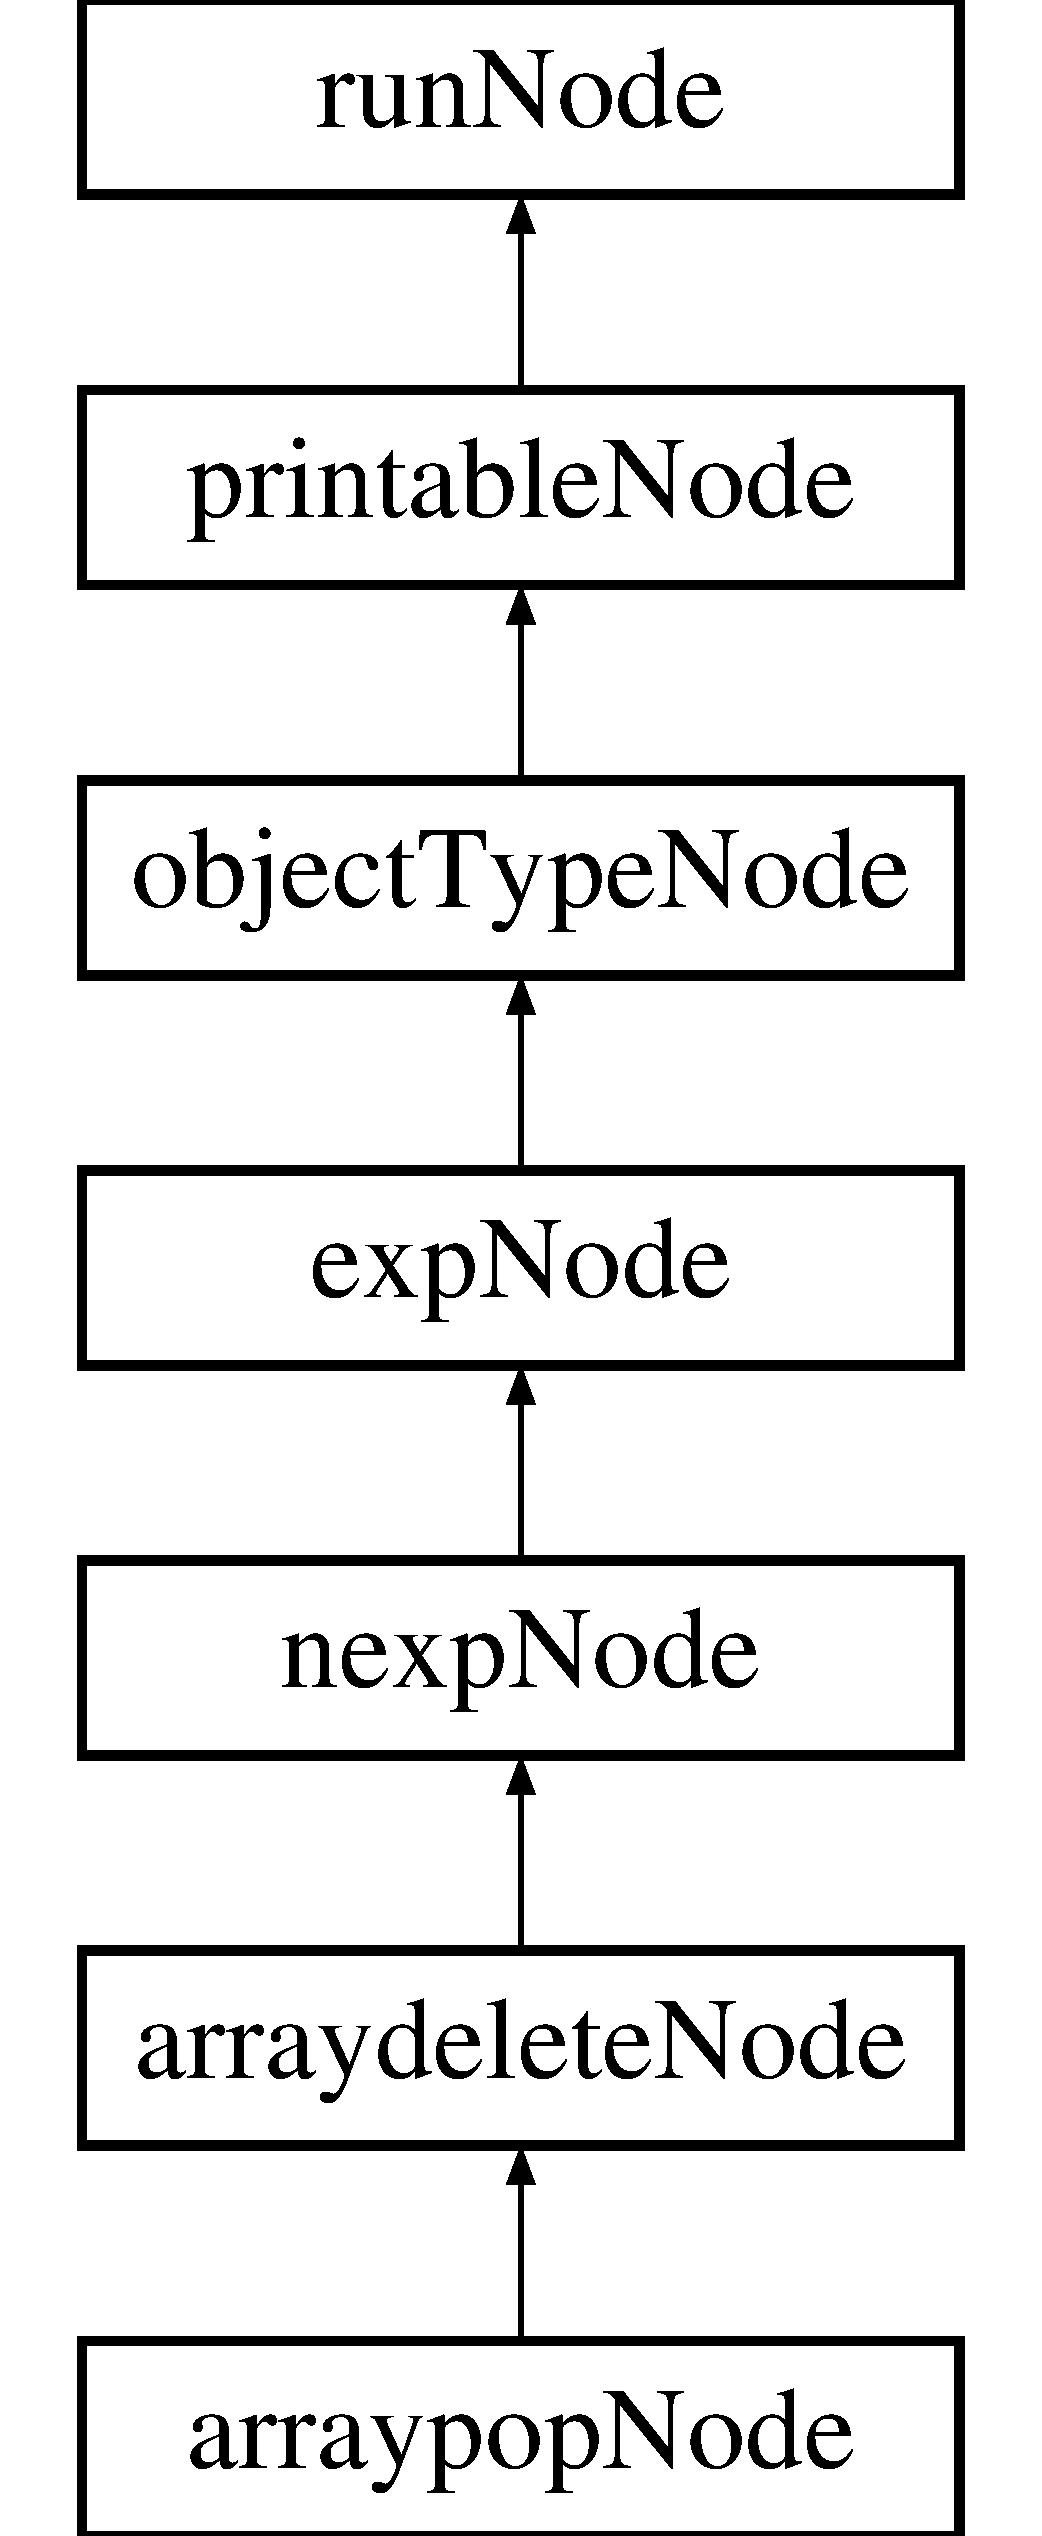
\includegraphics[height=7.000000cm]{classarraypopNode}
\end{center}
\end{figure}
\subsection*{Métodos públicos}
\begin{DoxyCompactItemize}
\item 
\hyperlink{classarraypopNode_a728f90285d083e62396e4d6b72684d90}{arraypop\-Node} (\hyperlink{classrunNode}{run\-Node} $\ast$array)
\item 
void \hyperlink{classarraypopNode_a5a96f6ab8867ca653bbe74ec8f4c1d4b}{run} ()
\end{DoxyCompactItemize}
\subsection*{Métodos públicos estáticos}
\begin{DoxyCompactItemize}
\item 
static \hyperlink{classrunNode}{run\-Node} $\ast$ \hyperlink{classarraypopNode_a5a6ac267a6db71b6d3e0b64657e81d34}{as\-Method} ()
\end{DoxyCompactItemize}


\subsection{Descripción detallada}
Nodo función elimina y devuelve el último elemento de array. 

La ejecución de este nodo elimina el último elemento de un array tras tomarlo como valor. 

\subsection{Documentación del constructor y destructor}
\hypertarget{classarraypopNode_a728f90285d083e62396e4d6b72684d90}{\index{arraypop\-Node@{arraypop\-Node}!arraypop\-Node@{arraypop\-Node}}
\index{arraypop\-Node@{arraypop\-Node}!arraypopNode@{arraypop\-Node}}
\subsubsection[{arraypop\-Node}]{\setlength{\rightskip}{0pt plus 5cm}arraypop\-Node\-::arraypop\-Node (
\begin{DoxyParamCaption}
\item[{{\bf run\-Node} $\ast$}]{array}
\end{DoxyParamCaption}
)}}\label{classarraypopNode_a728f90285d083e62396e4d6b72684d90}
Constructor de la clase. 
\begin{DoxyParams}{Parámetros}
{\em array} & Nodo que representa el array de elementos. \\
\hline
\end{DoxyParams}


\subsection{Documentación de las funciones miembro}
\hypertarget{classarraypopNode_a5a6ac267a6db71b6d3e0b64657e81d34}{\index{arraypop\-Node@{arraypop\-Node}!as\-Method@{as\-Method}}
\index{as\-Method@{as\-Method}!arraypopNode@{arraypop\-Node}}
\subsubsection[{as\-Method}]{\setlength{\rightskip}{0pt plus 5cm}{\bf run\-Node} $\ast$ arraypop\-Node\-::as\-Method (
\begin{DoxyParamCaption}
{}
\end{DoxyParamCaption}
)\hspace{0.3cm}{\ttfamily [static]}}}\label{classarraypopNode_a5a6ac267a6db71b6d3e0b64657e81d34}
Devuelve un nodo elimina y devuelve el último elemento de array como cuerpo de un nodo función, siendo un nodo this el array de elementos. \begin{DoxyReturn}{Devuelve}
Método pop. 
\end{DoxyReturn}
\hypertarget{classarraypopNode_a5a96f6ab8867ca653bbe74ec8f4c1d4b}{\index{arraypop\-Node@{arraypop\-Node}!run@{run}}
\index{run@{run}!arraypopNode@{arraypop\-Node}}
\subsubsection[{run}]{\setlength{\rightskip}{0pt plus 5cm}void arraypop\-Node\-::run (
\begin{DoxyParamCaption}
{}
\end{DoxyParamCaption}
)\hspace{0.3cm}{\ttfamily [virtual]}}}\label{classarraypopNode_a5a96f6ab8867ca653bbe74ec8f4c1d4b}
Método que ejecuta el nodo. Toma como valor el último elemento de un array y lo elimina del mismo. Si el array está vacío toma como valor un nodo nulo. 

Reimplementado de \hyperlink{classarraydeleteNode_a0ce9f89cbb1485472f071b3573f0477d}{arraydelete\-Node}.



La documentación para esta clase fue generada a partir de los siguientes ficheros\-:\begin{DoxyCompactItemize}
\item 
trunk/src/run/operators/\hyperlink{arrayOpNode_8h}{array\-Op\-Node.\-h}\item 
trunk/src/run/operators/array\-Op\-Node.\-cpp\end{DoxyCompactItemize}

\hypertarget{classarraypushNode}{\section{Referencia de la Clase arraypush\-Node}
\label{classarraypushNode}\index{arraypush\-Node@{arraypush\-Node}}
}


Nodo funcion inserta al final del array.  




{\ttfamily \#include $<$array\-Op\-Node.\-h$>$}

Diagrama de herencias de arraypush\-Node\begin{figure}[H]
\begin{center}
\leavevmode
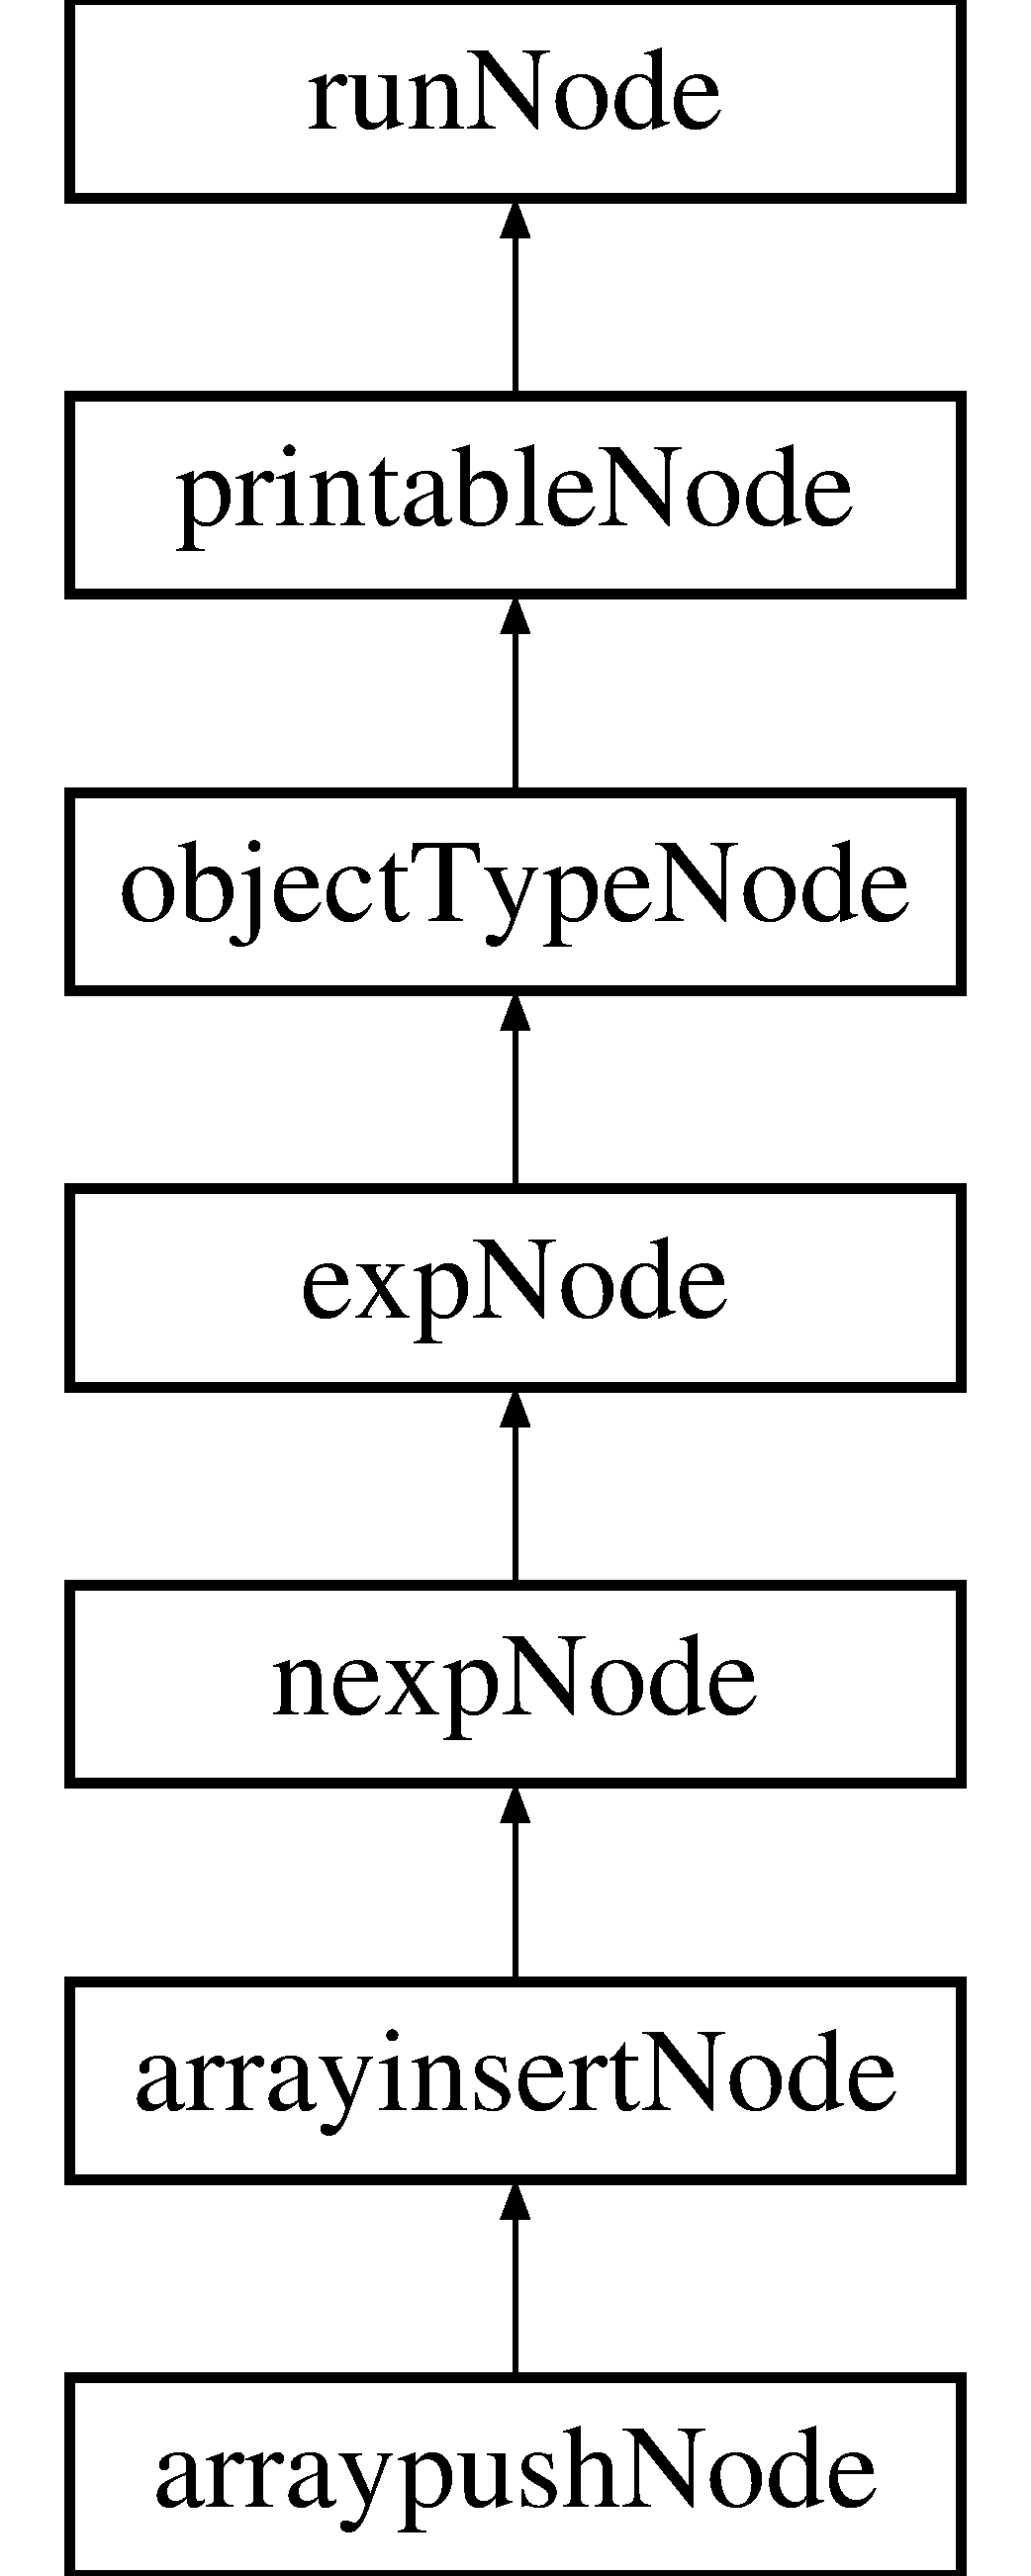
\includegraphics[height=7.000000cm]{classarraypushNode}
\end{center}
\end{figure}
\subsection*{Métodos públicos}
\begin{DoxyCompactItemize}
\item 
\hyperlink{classarraypushNode_ae2b0715919f55da61278a0469db2d1dd}{arraypush\-Node} (\hyperlink{classrunNode}{run\-Node} $\ast$array, \hyperlink{classrunNode}{run\-Node} $\ast$element)
\item 
void \hyperlink{classarraypushNode_a6eb706763d3f8cc7715706005d4bf049}{run} ()
\end{DoxyCompactItemize}
\subsection*{Métodos públicos estáticos}
\begin{DoxyCompactItemize}
\item 
static \hyperlink{classrunNode}{run\-Node} $\ast$ \hyperlink{classarraypushNode_afa60c2664e930e0f6328ad9f4086d65e}{as\-Method} ()
\end{DoxyCompactItemize}


\subsection{Descripción detallada}
Nodo funcion inserta al final del array. 

Este nodo se encarga de insertar un elemento al final de un array de elementos 

\subsection{Documentación del constructor y destructor}
\hypertarget{classarraypushNode_ae2b0715919f55da61278a0469db2d1dd}{\index{arraypush\-Node@{arraypush\-Node}!arraypush\-Node@{arraypush\-Node}}
\index{arraypush\-Node@{arraypush\-Node}!arraypushNode@{arraypush\-Node}}
\subsubsection[{arraypush\-Node}]{\setlength{\rightskip}{0pt plus 5cm}arraypush\-Node\-::arraypush\-Node (
\begin{DoxyParamCaption}
\item[{{\bf run\-Node} $\ast$}]{array, }
\item[{{\bf run\-Node} $\ast$}]{element}
\end{DoxyParamCaption}
)}}\label{classarraypushNode_ae2b0715919f55da61278a0469db2d1dd}
Constructor de la clase 
\begin{DoxyParams}{Parámetros}
{\em array} & Nodo que representa el array de elementos \\
\hline
{\em element} & Nodo que representa el elemento a insertar \\
\hline
\end{DoxyParams}


\subsection{Documentación de las funciones miembro}
\hypertarget{classarraypushNode_afa60c2664e930e0f6328ad9f4086d65e}{\index{arraypush\-Node@{arraypush\-Node}!as\-Method@{as\-Method}}
\index{as\-Method@{as\-Method}!arraypushNode@{arraypush\-Node}}
\subsubsection[{as\-Method}]{\setlength{\rightskip}{0pt plus 5cm}{\bf run\-Node} $\ast$ arraypush\-Node\-::as\-Method (
\begin{DoxyParamCaption}
{}
\end{DoxyParamCaption}
)\hspace{0.3cm}{\ttfamily [static]}}}\label{classarraypushNode_afa60c2664e930e0f6328ad9f4086d65e}
Devuelve un nodo inserta al final del array como cuerpo de un nodo función, siendo un nodo this el array de elementos. \begin{DoxyReturn}{Devuelve}
Método push. 
\end{DoxyReturn}
\hypertarget{classarraypushNode_a6eb706763d3f8cc7715706005d4bf049}{\index{arraypush\-Node@{arraypush\-Node}!run@{run}}
\index{run@{run}!arraypushNode@{arraypush\-Node}}
\subsubsection[{run}]{\setlength{\rightskip}{0pt plus 5cm}void arraypush\-Node\-::run (
\begin{DoxyParamCaption}
{}
\end{DoxyParamCaption}
)\hspace{0.3cm}{\ttfamily [virtual]}}}\label{classarraypushNode_a6eb706763d3f8cc7715706005d4bf049}
Método que ejecuta el nodo. Inserta el elemento al final del array. Se toma como valor una referencia al array con el elemento insertado, 

Reimplementado de \hyperlink{classarrayinsertNode_a1a72ddaf1ade1ee8a535ae1ca1fc2861}{arrayinsert\-Node}.



La documentación para esta clase fue generada a partir de los siguientes ficheros\-:\begin{DoxyCompactItemize}
\item 
trunk/src/run/operators/\hyperlink{arrayOpNode_8h}{array\-Op\-Node.\-h}\item 
trunk/src/run/operators/array\-Op\-Node.\-cpp\end{DoxyCompactItemize}

\hypertarget{classarrayshiftNode}{\section{Referencia de la Clase arrayshift\-Node}
\label{classarrayshiftNode}\index{arrayshift\-Node@{arrayshift\-Node}}
}


Nodo función elimina y devuelve el primer elemento de array.  




{\ttfamily \#include $<$array\-Op\-Node.\-h$>$}

Diagrama de herencias de arrayshift\-Node\begin{figure}[H]
\begin{center}
\leavevmode
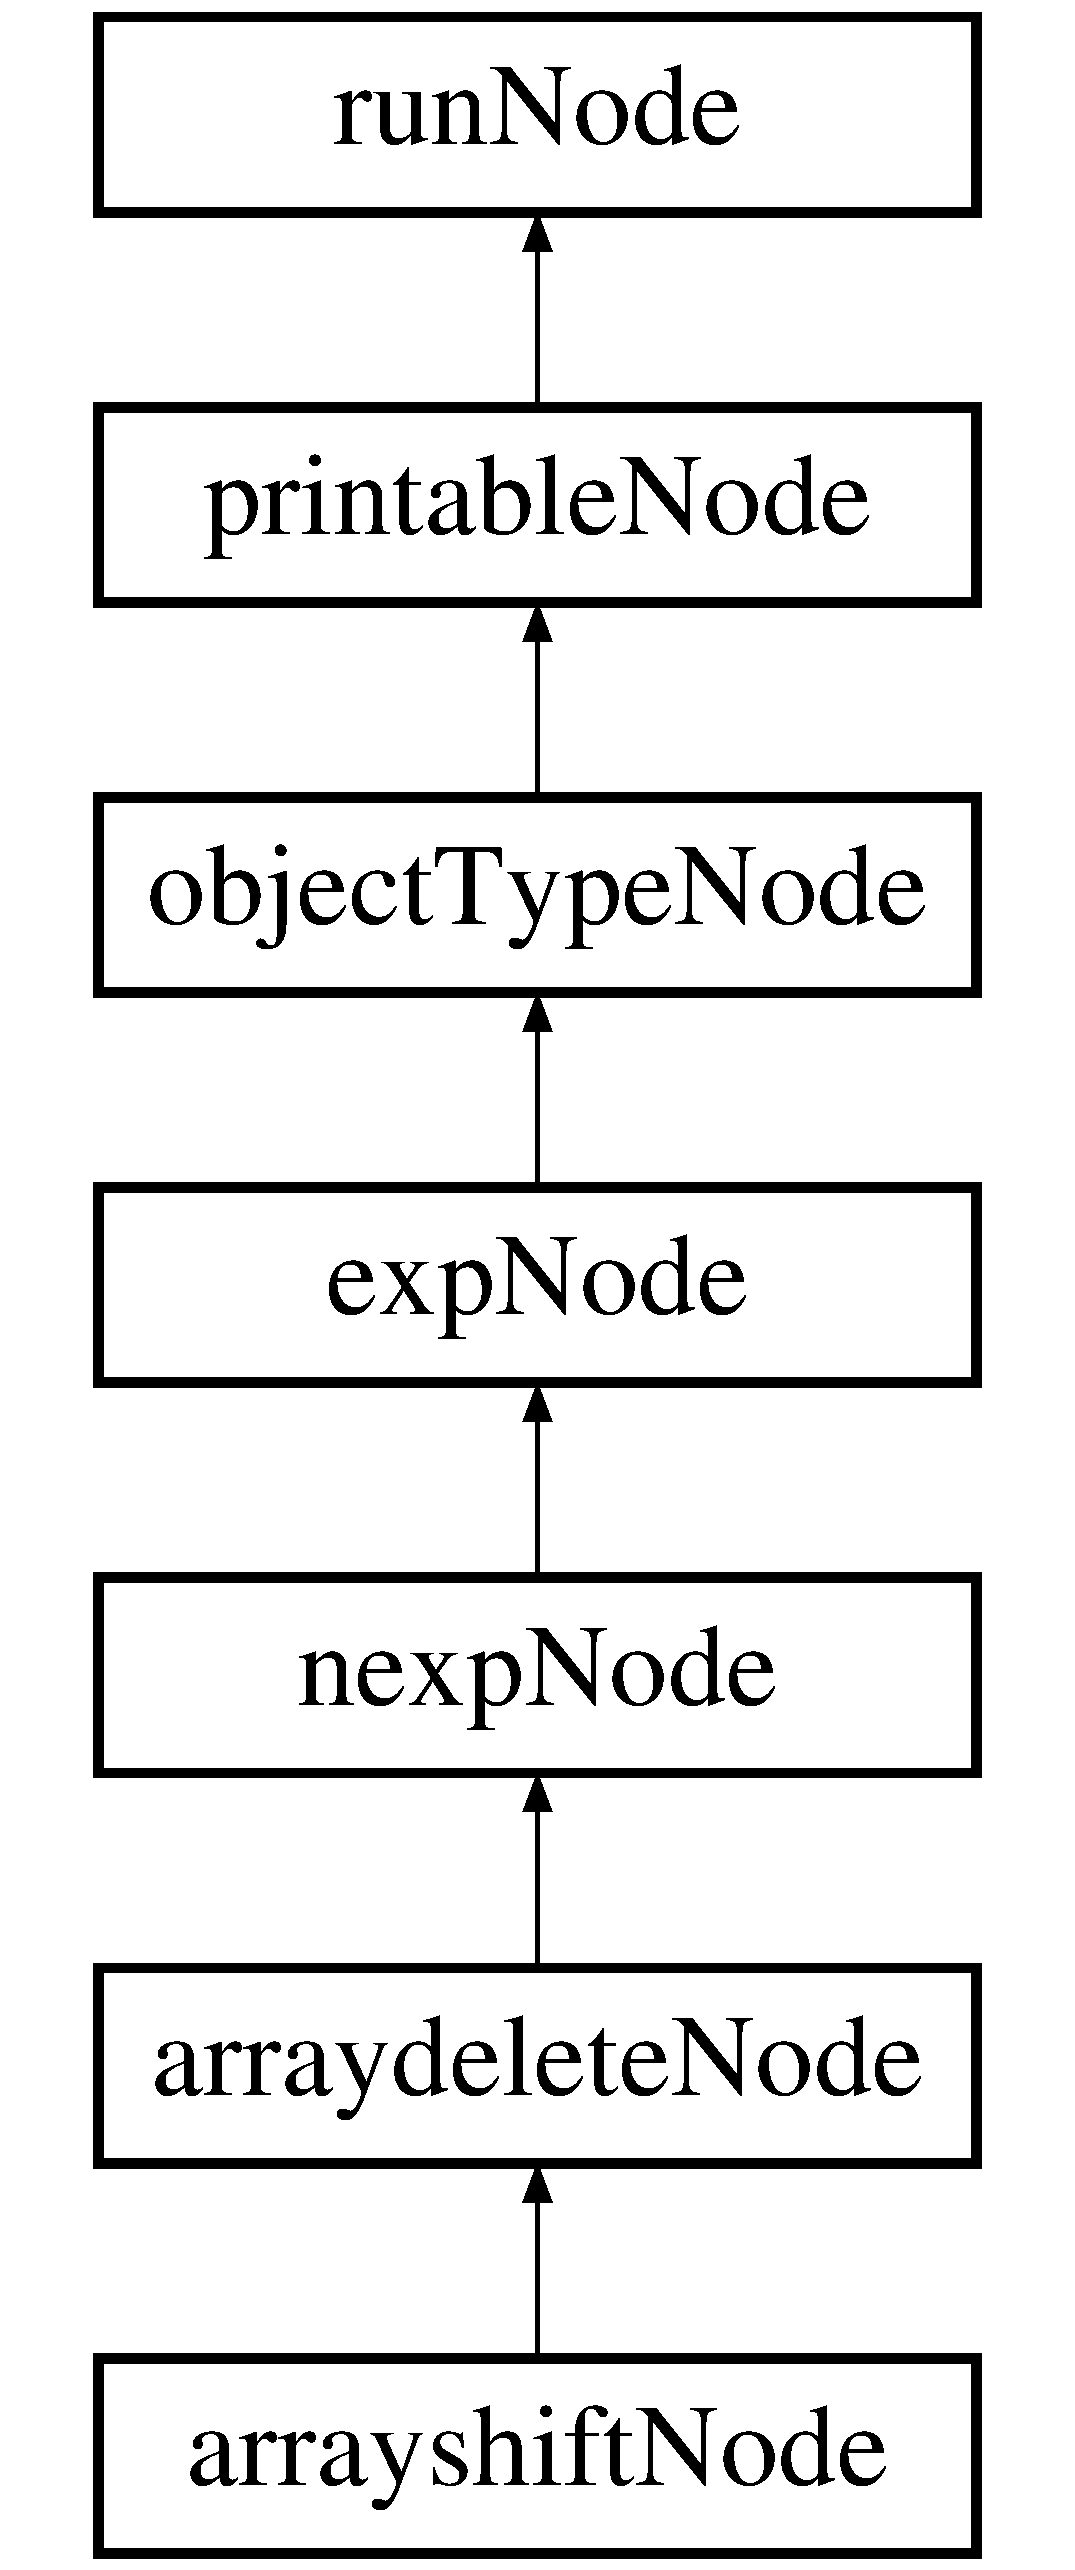
\includegraphics[height=7.000000cm]{classarrayshiftNode}
\end{center}
\end{figure}
\subsection*{Métodos públicos}
\begin{DoxyCompactItemize}
\item 
\hyperlink{classarrayshiftNode_accfc038b2d871cbc2b5cb22c70442e0d}{arrayshift\-Node} (\hyperlink{classrunNode}{run\-Node} $\ast$array)
\item 
void \hyperlink{classarrayshiftNode_a2a34028d6f0763c7df0220ef2c624580}{run} ()
\end{DoxyCompactItemize}
\subsection*{Métodos públicos estáticos}
\begin{DoxyCompactItemize}
\item 
static \hyperlink{classrunNode}{run\-Node} $\ast$ \hyperlink{classarrayshiftNode_a83eac7bc2860d5b1bc4969ff00a85e77}{as\-Method} ()
\end{DoxyCompactItemize}


\subsection{Descripción detallada}
Nodo función elimina y devuelve el primer elemento de array. 

La ejecución de este nodo elimina el primer elemento de un array tras tomarlo como valor. 

\subsection{Documentación del constructor y destructor}
\hypertarget{classarrayshiftNode_accfc038b2d871cbc2b5cb22c70442e0d}{\index{arrayshift\-Node@{arrayshift\-Node}!arrayshift\-Node@{arrayshift\-Node}}
\index{arrayshift\-Node@{arrayshift\-Node}!arrayshiftNode@{arrayshift\-Node}}
\subsubsection[{arrayshift\-Node}]{\setlength{\rightskip}{0pt plus 5cm}arrayshift\-Node\-::arrayshift\-Node (
\begin{DoxyParamCaption}
\item[{{\bf run\-Node} $\ast$}]{array}
\end{DoxyParamCaption}
)}}\label{classarrayshiftNode_accfc038b2d871cbc2b5cb22c70442e0d}
Constructor de la clase. 
\begin{DoxyParams}{Parámetros}
{\em array} & Nodo que representa el array de elementos. \\
\hline
\end{DoxyParams}


\subsection{Documentación de las funciones miembro}
\hypertarget{classarrayshiftNode_a83eac7bc2860d5b1bc4969ff00a85e77}{\index{arrayshift\-Node@{arrayshift\-Node}!as\-Method@{as\-Method}}
\index{as\-Method@{as\-Method}!arrayshiftNode@{arrayshift\-Node}}
\subsubsection[{as\-Method}]{\setlength{\rightskip}{0pt plus 5cm}{\bf run\-Node} $\ast$ arrayshift\-Node\-::as\-Method (
\begin{DoxyParamCaption}
{}
\end{DoxyParamCaption}
)\hspace{0.3cm}{\ttfamily [static]}}}\label{classarrayshiftNode_a83eac7bc2860d5b1bc4969ff00a85e77}
Devuelve un nodo elimina y devuelve el primer elemento de array como cuerpo de un nodo función, siendo un nodo this el array de elementos. \begin{DoxyReturn}{Devuelve}
Método shift. 
\end{DoxyReturn}
\hypertarget{classarrayshiftNode_a2a34028d6f0763c7df0220ef2c624580}{\index{arrayshift\-Node@{arrayshift\-Node}!run@{run}}
\index{run@{run}!arrayshiftNode@{arrayshift\-Node}}
\subsubsection[{run}]{\setlength{\rightskip}{0pt plus 5cm}void arrayshift\-Node\-::run (
\begin{DoxyParamCaption}
{}
\end{DoxyParamCaption}
)\hspace{0.3cm}{\ttfamily [virtual]}}}\label{classarrayshiftNode_a2a34028d6f0763c7df0220ef2c624580}
Método que ejecuta el nodo. Toma como valor el primer elemento de un array y lo elimina del mismo. Si el array está vacío toma como valor un nodo nulo. 

Reimplementado de \hyperlink{classarraydeleteNode_a0ce9f89cbb1485472f071b3573f0477d}{arraydelete\-Node}.



La documentación para esta clase fue generada a partir de los siguientes ficheros\-:\begin{DoxyCompactItemize}
\item 
trunk/src/run/operators/\hyperlink{arrayOpNode_8h}{array\-Op\-Node.\-h}\item 
trunk/src/run/operators/array\-Op\-Node.\-cpp\end{DoxyCompactItemize}

\hypertarget{classarrayunshiftNode}{\section{Referencia de la Clase arrayunshift\-Node}
\label{classarrayunshiftNode}\index{arrayunshift\-Node@{arrayunshift\-Node}}
}


Nodo función insertar al inicio de array.  




{\ttfamily \#include $<$array\-Op\-Node.\-h$>$}

Diagrama de herencias de arrayunshift\-Node\begin{figure}[H]
\begin{center}
\leavevmode
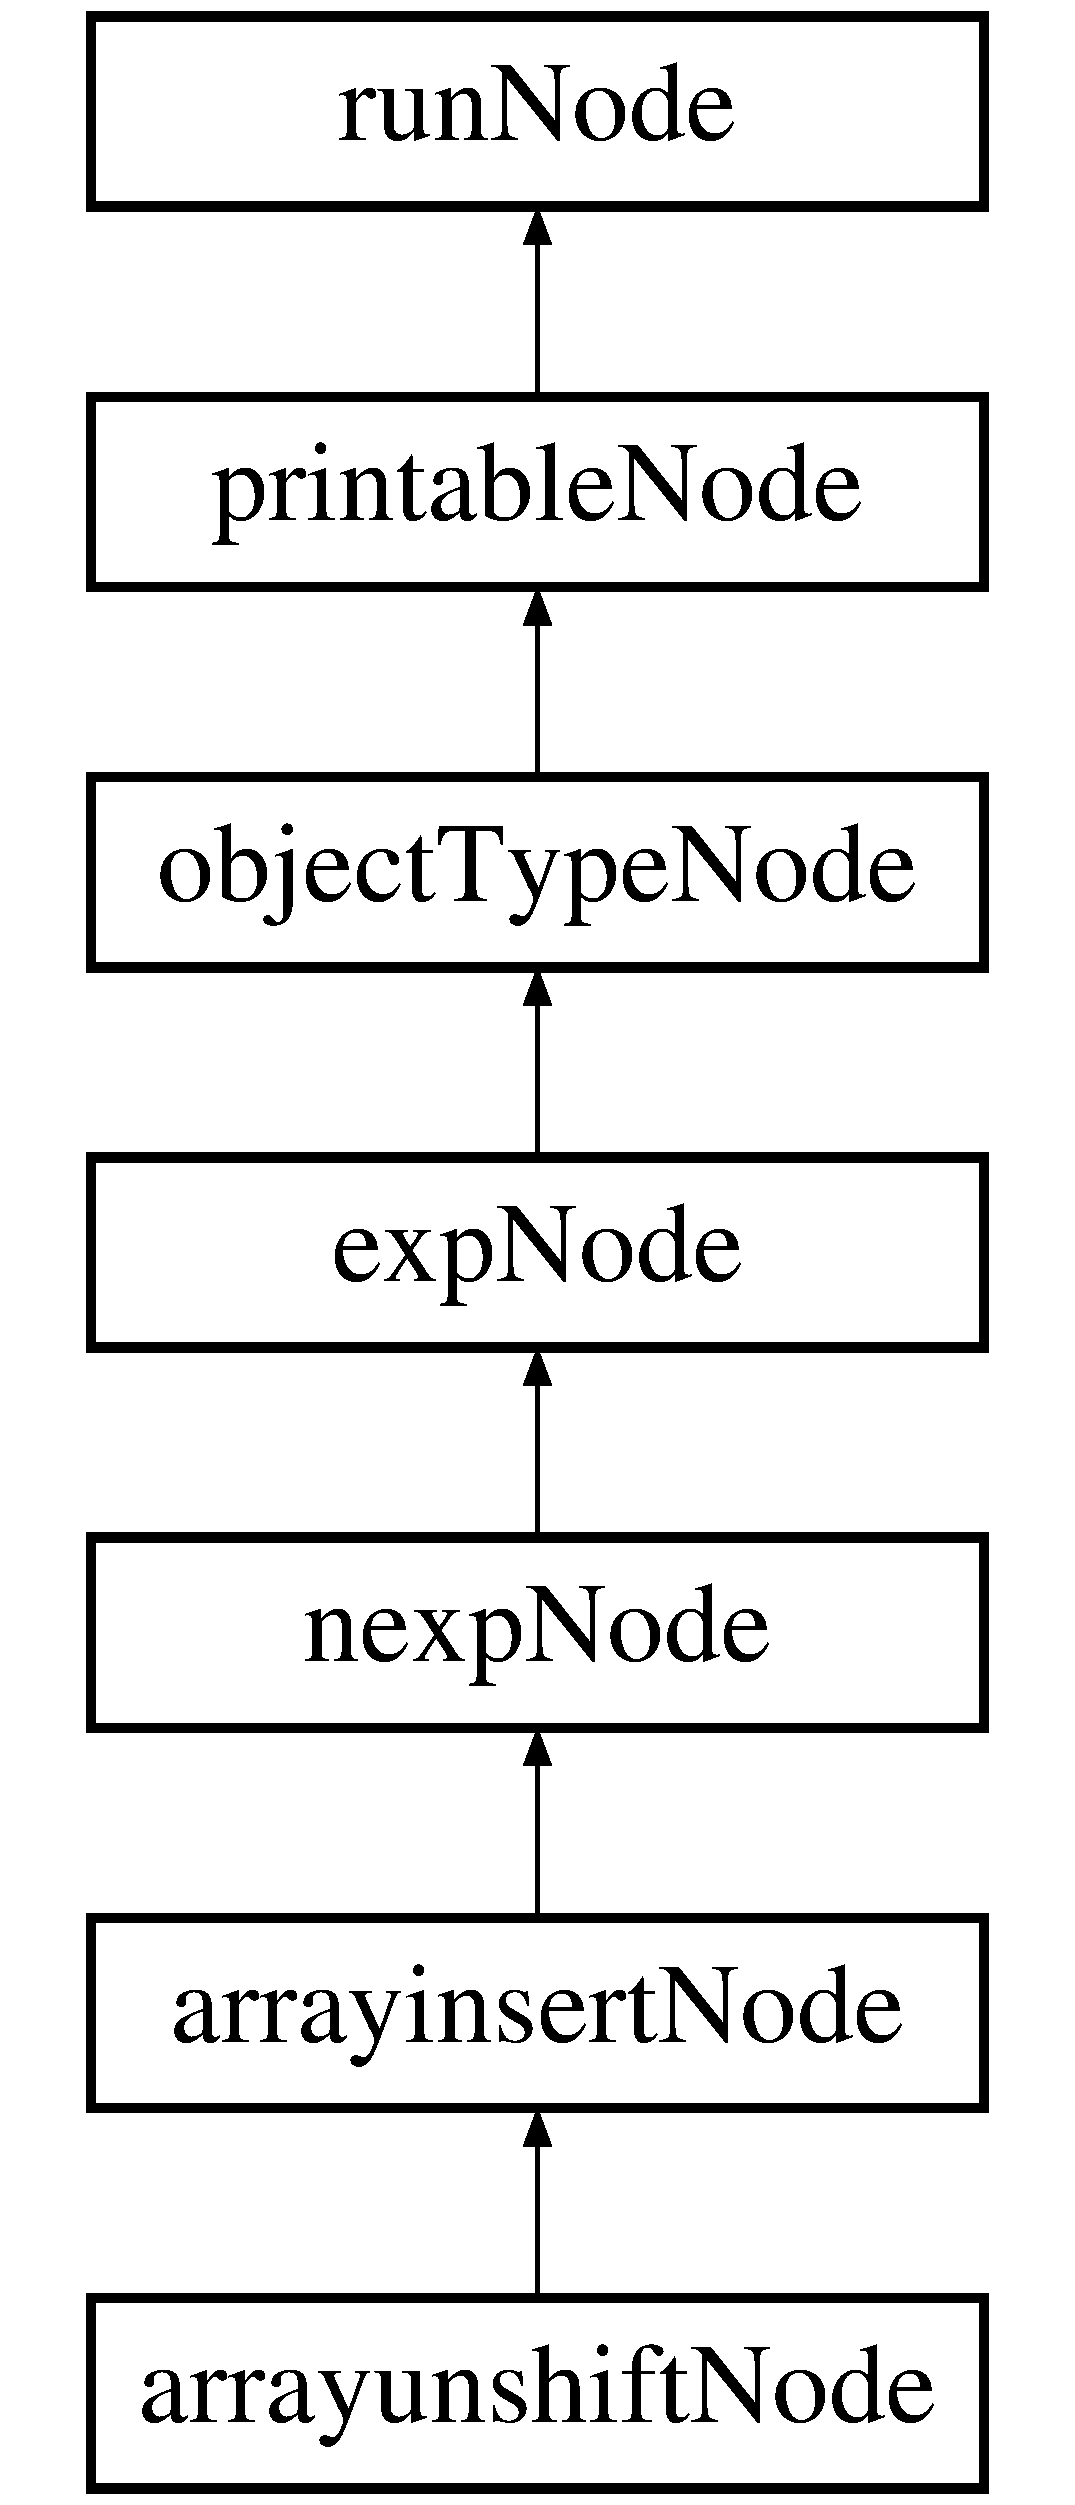
\includegraphics[height=7.000000cm]{classarrayunshiftNode}
\end{center}
\end{figure}
\subsection*{Métodos públicos}
\begin{DoxyCompactItemize}
\item 
\hyperlink{classarrayunshiftNode_af5da6d19f37b71f2daf3cac637c4b569}{arrayunshift\-Node} (\hyperlink{classrunNode}{run\-Node} $\ast$array, \hyperlink{classrunNode}{run\-Node} $\ast$element)
\end{DoxyCompactItemize}
\subsection*{Métodos públicos estáticos}
\begin{DoxyCompactItemize}
\item 
static \hyperlink{classrunNode}{run\-Node} $\ast$ \hyperlink{classarrayunshiftNode_a1f422544b724e343d01fd84d227daad0}{as\-Method} ()
\end{DoxyCompactItemize}


\subsection{Descripción detallada}
Nodo función insertar al inicio de array. 

Inserta un determindo elemento al inicio de un array. 

\subsection{Documentación del constructor y destructor}
\hypertarget{classarrayunshiftNode_af5da6d19f37b71f2daf3cac637c4b569}{\index{arrayunshift\-Node@{arrayunshift\-Node}!arrayunshift\-Node@{arrayunshift\-Node}}
\index{arrayunshift\-Node@{arrayunshift\-Node}!arrayunshiftNode@{arrayunshift\-Node}}
\subsubsection[{arrayunshift\-Node}]{\setlength{\rightskip}{0pt plus 5cm}arrayunshift\-Node\-::arrayunshift\-Node (
\begin{DoxyParamCaption}
\item[{{\bf run\-Node} $\ast$}]{array, }
\item[{{\bf run\-Node} $\ast$}]{element}
\end{DoxyParamCaption}
)}}\label{classarrayunshiftNode_af5da6d19f37b71f2daf3cac637c4b569}
Constructor de la clase 
\begin{DoxyParams}{Parámetros}
{\em array} & Nodo que prepresenta el array de elementos \\
\hline
{\em element} & Nodo que representa el elemento a insertar \\
\hline
\end{DoxyParams}


\subsection{Documentación de las funciones miembro}
\hypertarget{classarrayunshiftNode_a1f422544b724e343d01fd84d227daad0}{\index{arrayunshift\-Node@{arrayunshift\-Node}!as\-Method@{as\-Method}}
\index{as\-Method@{as\-Method}!arrayunshiftNode@{arrayunshift\-Node}}
\subsubsection[{as\-Method}]{\setlength{\rightskip}{0pt plus 5cm}{\bf run\-Node} $\ast$ arrayunshift\-Node\-::as\-Method (
\begin{DoxyParamCaption}
{}
\end{DoxyParamCaption}
)\hspace{0.3cm}{\ttfamily [static]}}}\label{classarrayunshiftNode_a1f422544b724e343d01fd84d227daad0}
Devuelve un nodo insertar al inicio de array como cuerpo de un nodo función, siendo un nodo this el array de elementos. \begin{DoxyReturn}{Devuelve}
Método unshift. 
\end{DoxyReturn}


La documentación para esta clase fue generada a partir de los siguientes ficheros\-:\begin{DoxyCompactItemize}
\item 
trunk/src/run/operators/\hyperlink{arrayOpNode_8h}{array\-Op\-Node.\-h}\item 
trunk/src/run/operators/array\-Op\-Node.\-cpp\end{DoxyCompactItemize}

\hypertarget{classasigdecNode}{\section{Referencia de la Clase asigdec\-Node}
\label{classasigdecNode}\index{asigdec\-Node@{asigdec\-Node}}
}


Nodo operador asignación y decremento.  




{\ttfamily \#include $<$arith\-Op\-Node.\-h$>$}

Diagrama de herencias de asigdec\-Node\begin{figure}[H]
\begin{center}
\leavevmode
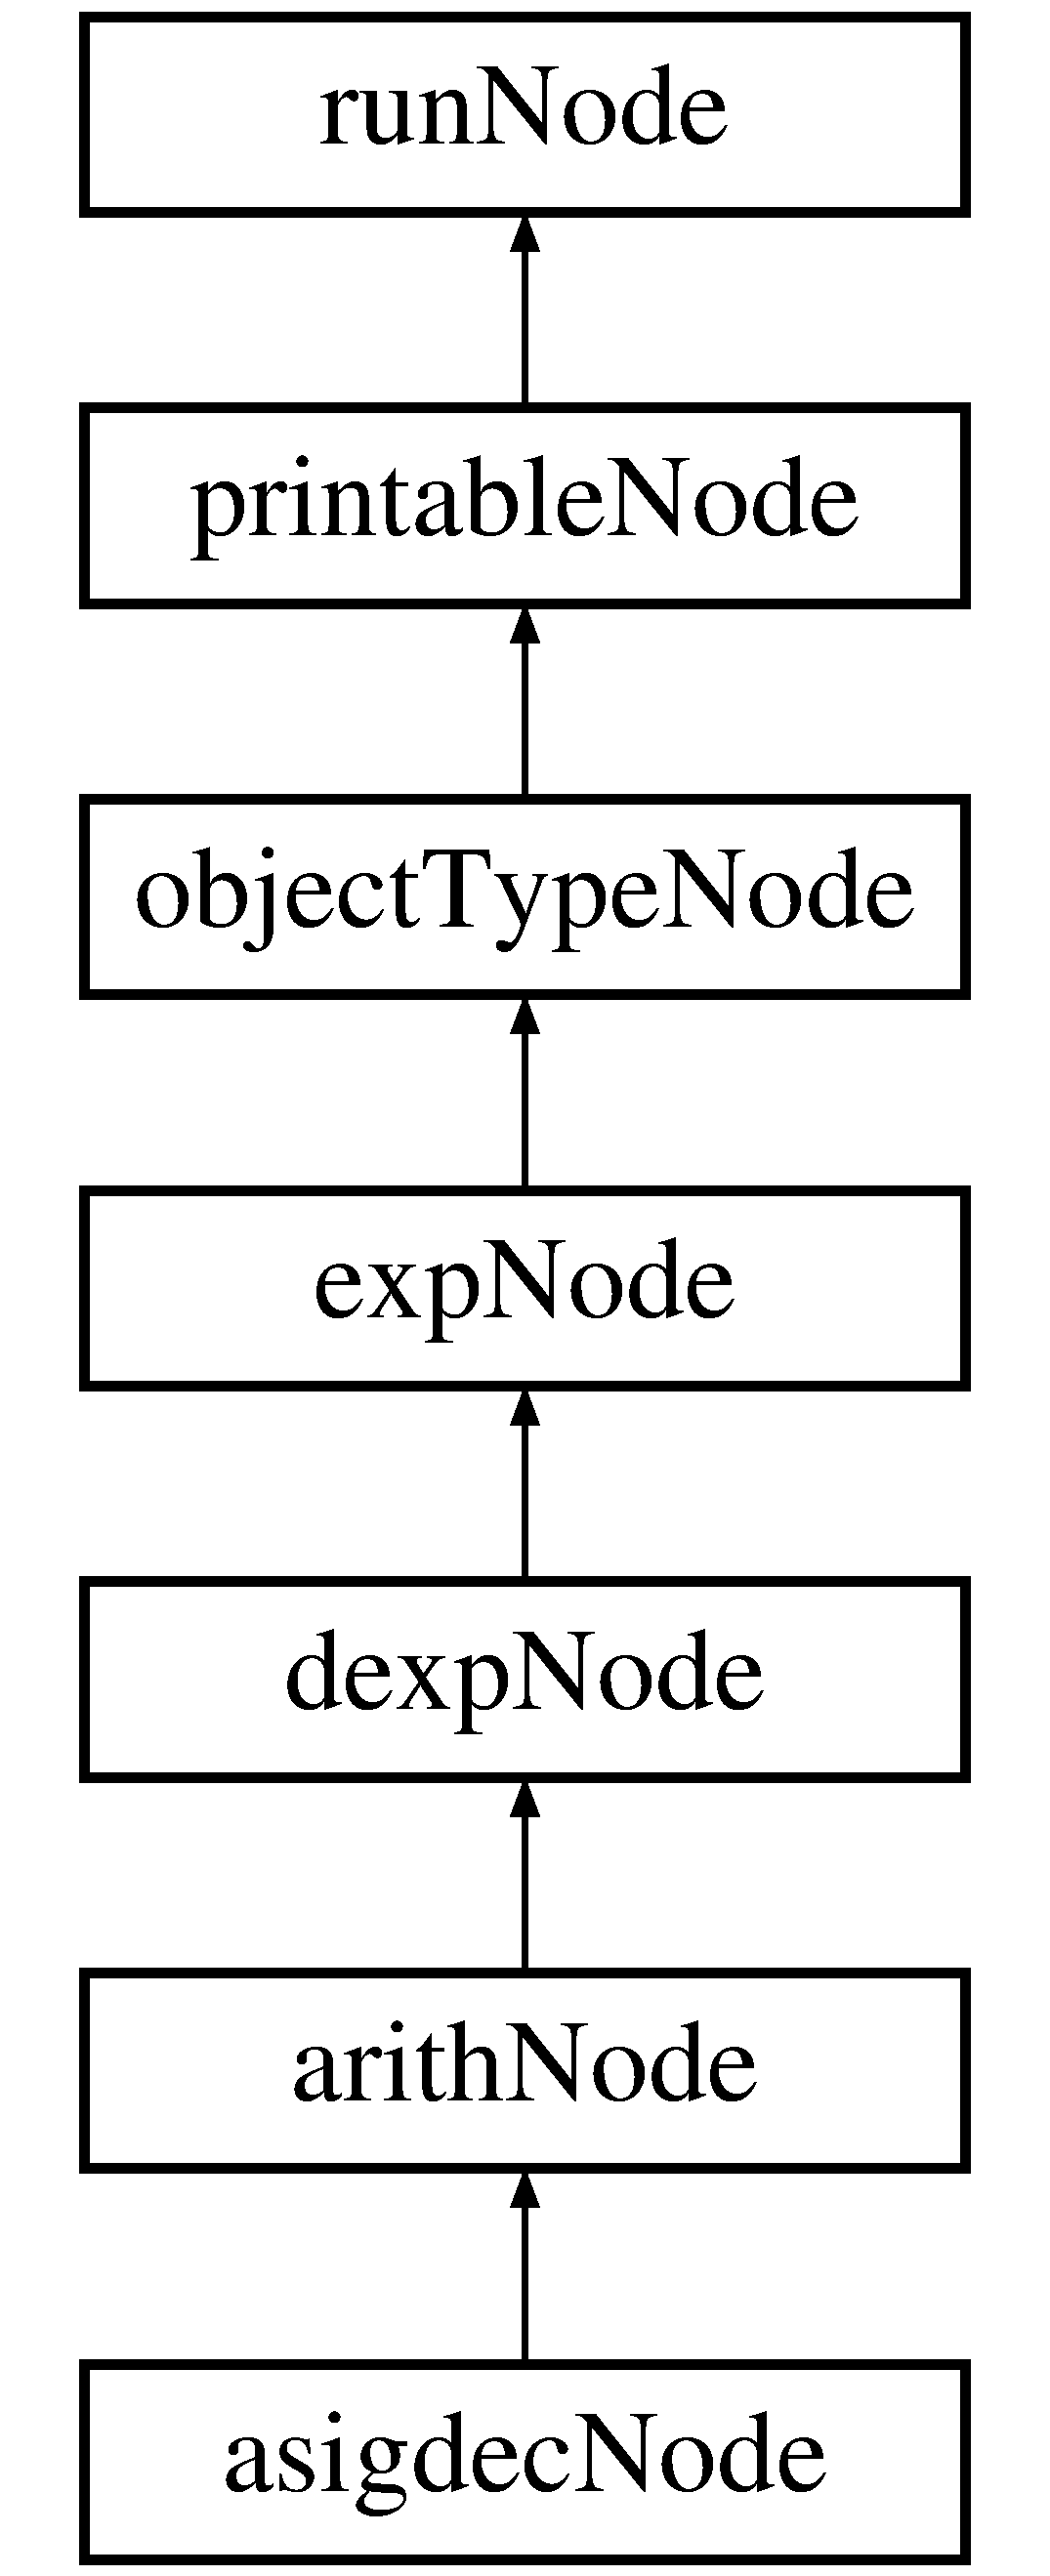
\includegraphics[height=7.000000cm]{classasigdecNode}
\end{center}
\end{figure}
\subsection*{Métodos públicos}
\begin{DoxyCompactItemize}
\item 
\hyperlink{classasigdecNode_ac3ec554aeeee40c2ecd063f856796af8}{asigdec\-Node} (\hyperlink{classrunNode}{run\-Node} $\ast$node)
\item 
void \hyperlink{classasigdecNode_a64dcc521a5b122854a4736943823e82c}{run} ()
\end{DoxyCompactItemize}
\subsection*{Otros miembros heredados}


\subsection{Descripción detallada}
Nodo operador asignación y decremento. 

Este nodo implementa la operación asignación e decremento. Se toma el valor de el nodo asociado, que normalmente representará un símbolo variable, luego se decrementa el valor de este.

El resultado de evaluar la expresión es el valor antes de decrementar. 

\subsection{Documentación del constructor y destructor}
\hypertarget{classasigdecNode_ac3ec554aeeee40c2ecd063f856796af8}{\index{asigdec\-Node@{asigdec\-Node}!asigdec\-Node@{asigdec\-Node}}
\index{asigdec\-Node@{asigdec\-Node}!asigdecNode@{asigdec\-Node}}
\subsubsection[{asigdec\-Node}]{\setlength{\rightskip}{0pt plus 5cm}asigdec\-Node\-::asigdec\-Node (
\begin{DoxyParamCaption}
\item[{{\bf run\-Node} $\ast$}]{node}
\end{DoxyParamCaption}
)}}\label{classasigdecNode_ac3ec554aeeee40c2ecd063f856796af8}
Constructor de la clase. Asocia el nodo operador a un nodo. 
\begin{DoxyParams}{Parámetros}
{\em node} & Nodo operando. \\
\hline
\end{DoxyParams}


\subsection{Documentación de las funciones miembro}
\hypertarget{classasigdecNode_a64dcc521a5b122854a4736943823e82c}{\index{asigdec\-Node@{asigdec\-Node}!run@{run}}
\index{run@{run}!asigdecNode@{asigdec\-Node}}
\subsubsection[{run}]{\setlength{\rightskip}{0pt plus 5cm}void asigdec\-Node\-::run (
\begin{DoxyParamCaption}
{}
\end{DoxyParamCaption}
)\hspace{0.3cm}{\ttfamily [virtual]}}}\label{classasigdecNode_a64dcc521a5b122854a4736943823e82c}
Método que ejecuta el nodo. Asocia el valor del nodo operando como valor interno del operador. Luego procede a incrementar el valor del nodo asociado. 

Implementa \hyperlink{classrunNode_a83c10df8148829b08e04153c93d69eec}{run\-Node}.



La documentación para esta clase fue generada a partir de los siguientes ficheros\-:\begin{DoxyCompactItemize}
\item 
trunk/src/run/operators/\hyperlink{arithOpNode_8h}{arith\-Op\-Node.\-h}\item 
trunk/src/run/operators/arith\-Op\-Node.\-cpp\end{DoxyCompactItemize}

\hypertarget{classasigincNode}{\section{Referencia de la Clase asiginc\-Node}
\label{classasigincNode}\index{asiginc\-Node@{asiginc\-Node}}
}


Nodo operador asignación e incremento.  




{\ttfamily \#include $<$arith\-Op\-Node.\-h$>$}

Diagrama de herencias de asiginc\-Node\begin{figure}[H]
\begin{center}
\leavevmode
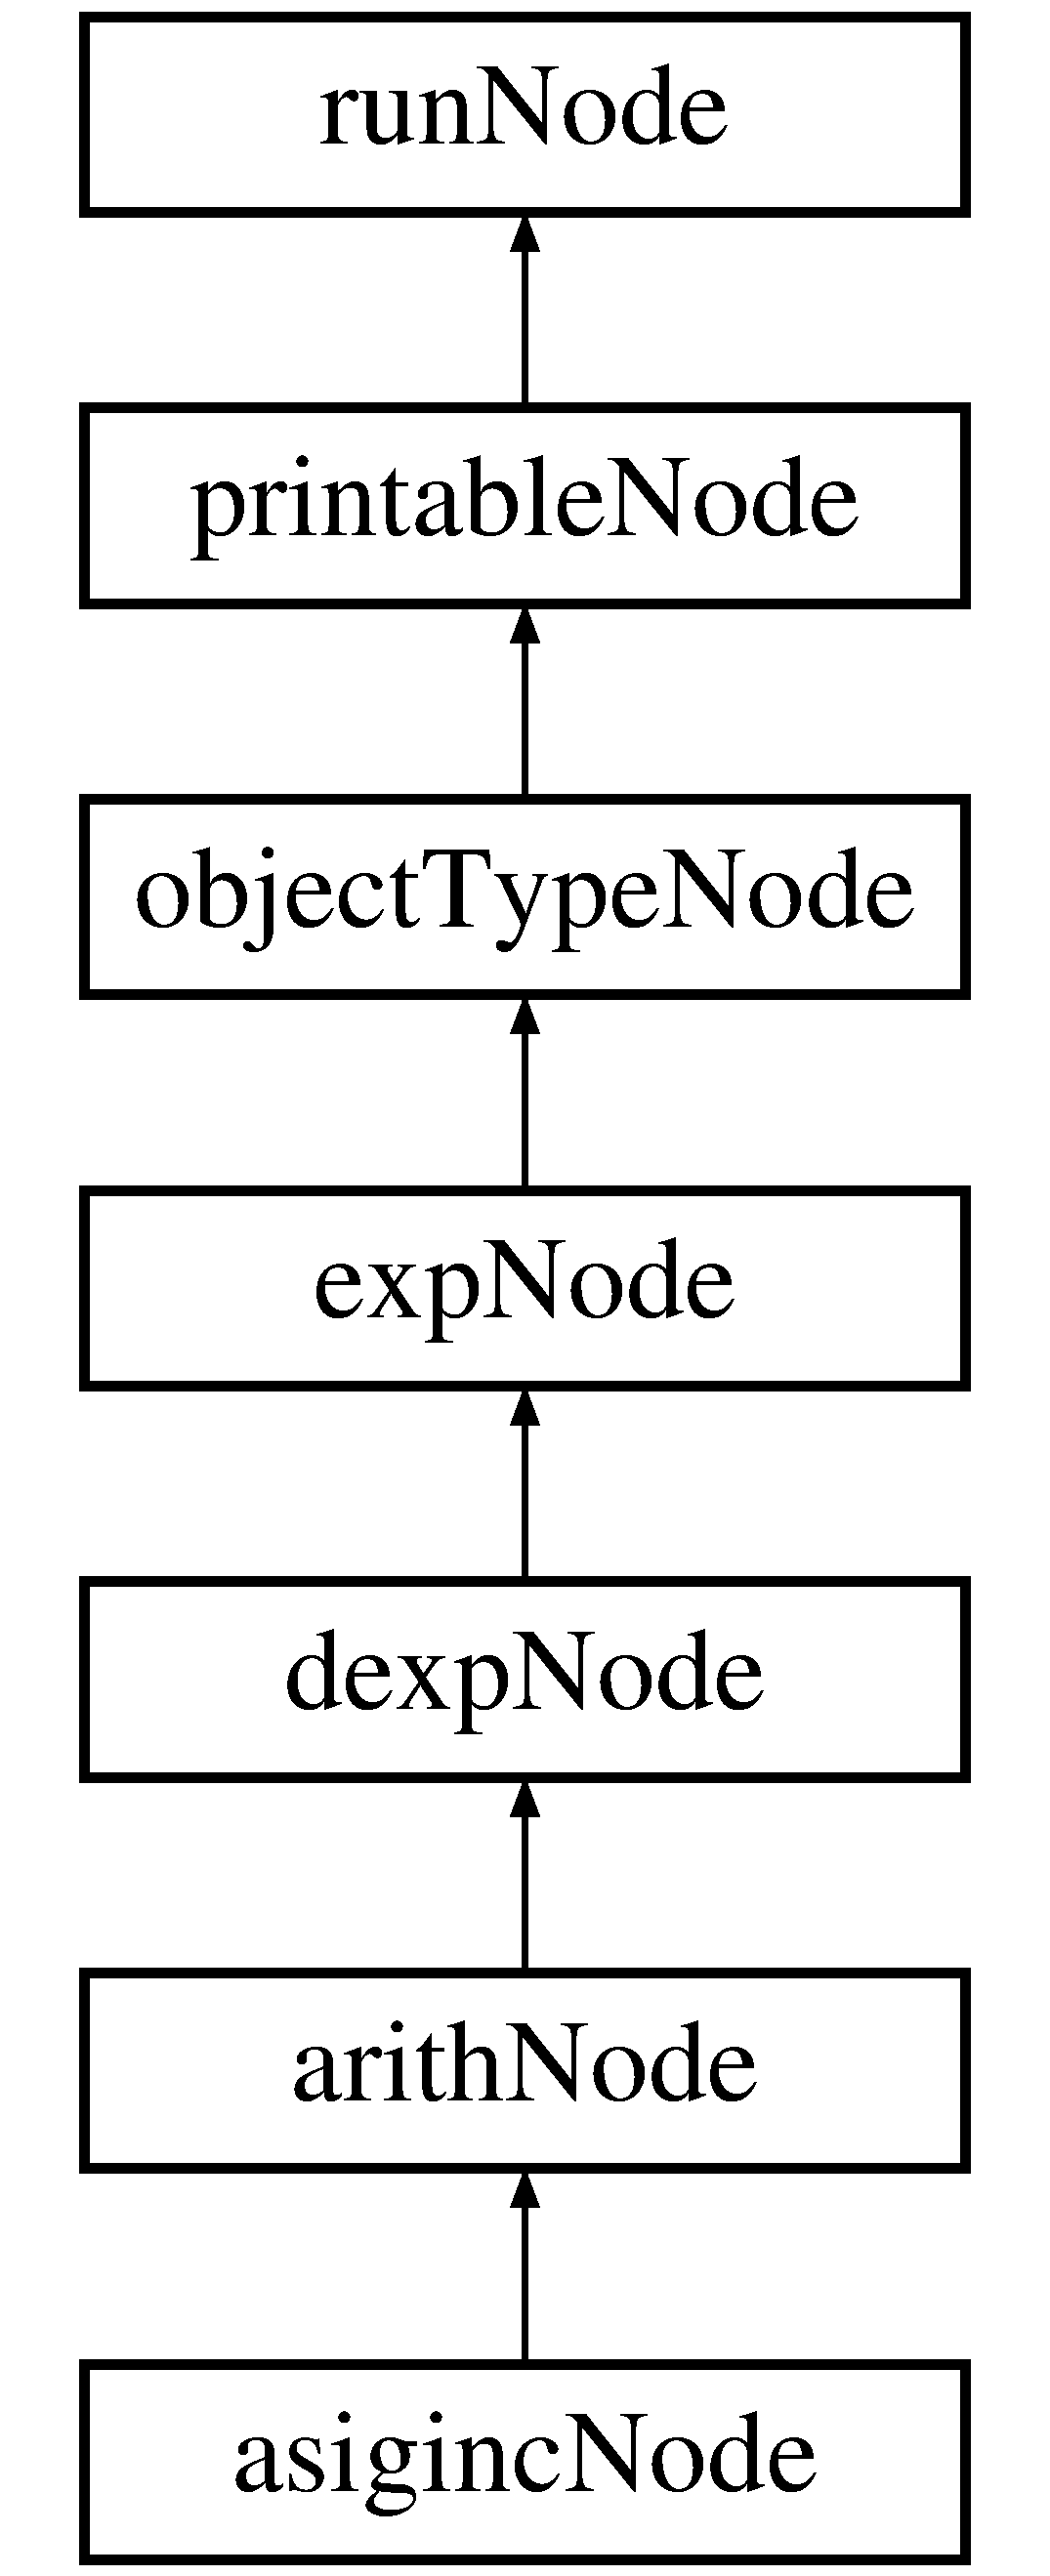
\includegraphics[height=7.000000cm]{classasigincNode}
\end{center}
\end{figure}
\subsection*{Métodos públicos}
\begin{DoxyCompactItemize}
\item 
\hyperlink{classasigincNode_a967172e05a123cff542f506b358827bb}{asiginc\-Node} (\hyperlink{classrunNode}{run\-Node} $\ast$node)
\item 
void \hyperlink{classasigincNode_abba913e2980459be1217172e294c1e22}{run} ()
\end{DoxyCompactItemize}
\subsection*{Otros miembros heredados}


\subsection{Descripción detallada}
Nodo operador asignación e incremento. 

Este nodo implementa la operación asignación e incremento. Se toma el valor de el nodo asociado, que normalmente representará un símbolo variable, luego se incrementa el valor de este.

El resultado de evaluar la expresión es el valor antes de incrementar. 

\subsection{Documentación del constructor y destructor}
\hypertarget{classasigincNode_a967172e05a123cff542f506b358827bb}{\index{asiginc\-Node@{asiginc\-Node}!asiginc\-Node@{asiginc\-Node}}
\index{asiginc\-Node@{asiginc\-Node}!asigincNode@{asiginc\-Node}}
\subsubsection[{asiginc\-Node}]{\setlength{\rightskip}{0pt plus 5cm}asiginc\-Node\-::asiginc\-Node (
\begin{DoxyParamCaption}
\item[{{\bf run\-Node} $\ast$}]{node}
\end{DoxyParamCaption}
)}}\label{classasigincNode_a967172e05a123cff542f506b358827bb}
Constructor de la clase. Asocia el nodo operador a un nodo. 
\begin{DoxyParams}{Parámetros}
{\em node} & Nodo operando. \\
\hline
\end{DoxyParams}


\subsection{Documentación de las funciones miembro}
\hypertarget{classasigincNode_abba913e2980459be1217172e294c1e22}{\index{asiginc\-Node@{asiginc\-Node}!run@{run}}
\index{run@{run}!asigincNode@{asiginc\-Node}}
\subsubsection[{run}]{\setlength{\rightskip}{0pt plus 5cm}void asiginc\-Node\-::run (
\begin{DoxyParamCaption}
{}
\end{DoxyParamCaption}
)\hspace{0.3cm}{\ttfamily [virtual]}}}\label{classasigincNode_abba913e2980459be1217172e294c1e22}
Método que ejecuta el nodo. Asocia el valor del nodo operando como valor interno del operador. Luego procede a incrementar el valor del nodo asociado. 

Implementa \hyperlink{classrunNode_a83c10df8148829b08e04153c93d69eec}{run\-Node}.



La documentación para esta clase fue generada a partir de los siguientes ficheros\-:\begin{DoxyCompactItemize}
\item 
trunk/src/run/operators/\hyperlink{arithOpNode_8h}{arith\-Op\-Node.\-h}\item 
trunk/src/run/operators/arith\-Op\-Node.\-cpp\end{DoxyCompactItemize}

\hypertarget{classasigNode}{\section{Referencia de la Clase asig\-Node}
\label{classasigNode}\index{asig\-Node@{asig\-Node}}
}


Nodo asignación.  




{\ttfamily \#include $<$symbol\-Op\-Node.\-h$>$}

Diagrama de herencias de asig\-Node\begin{figure}[H]
\begin{center}
\leavevmode
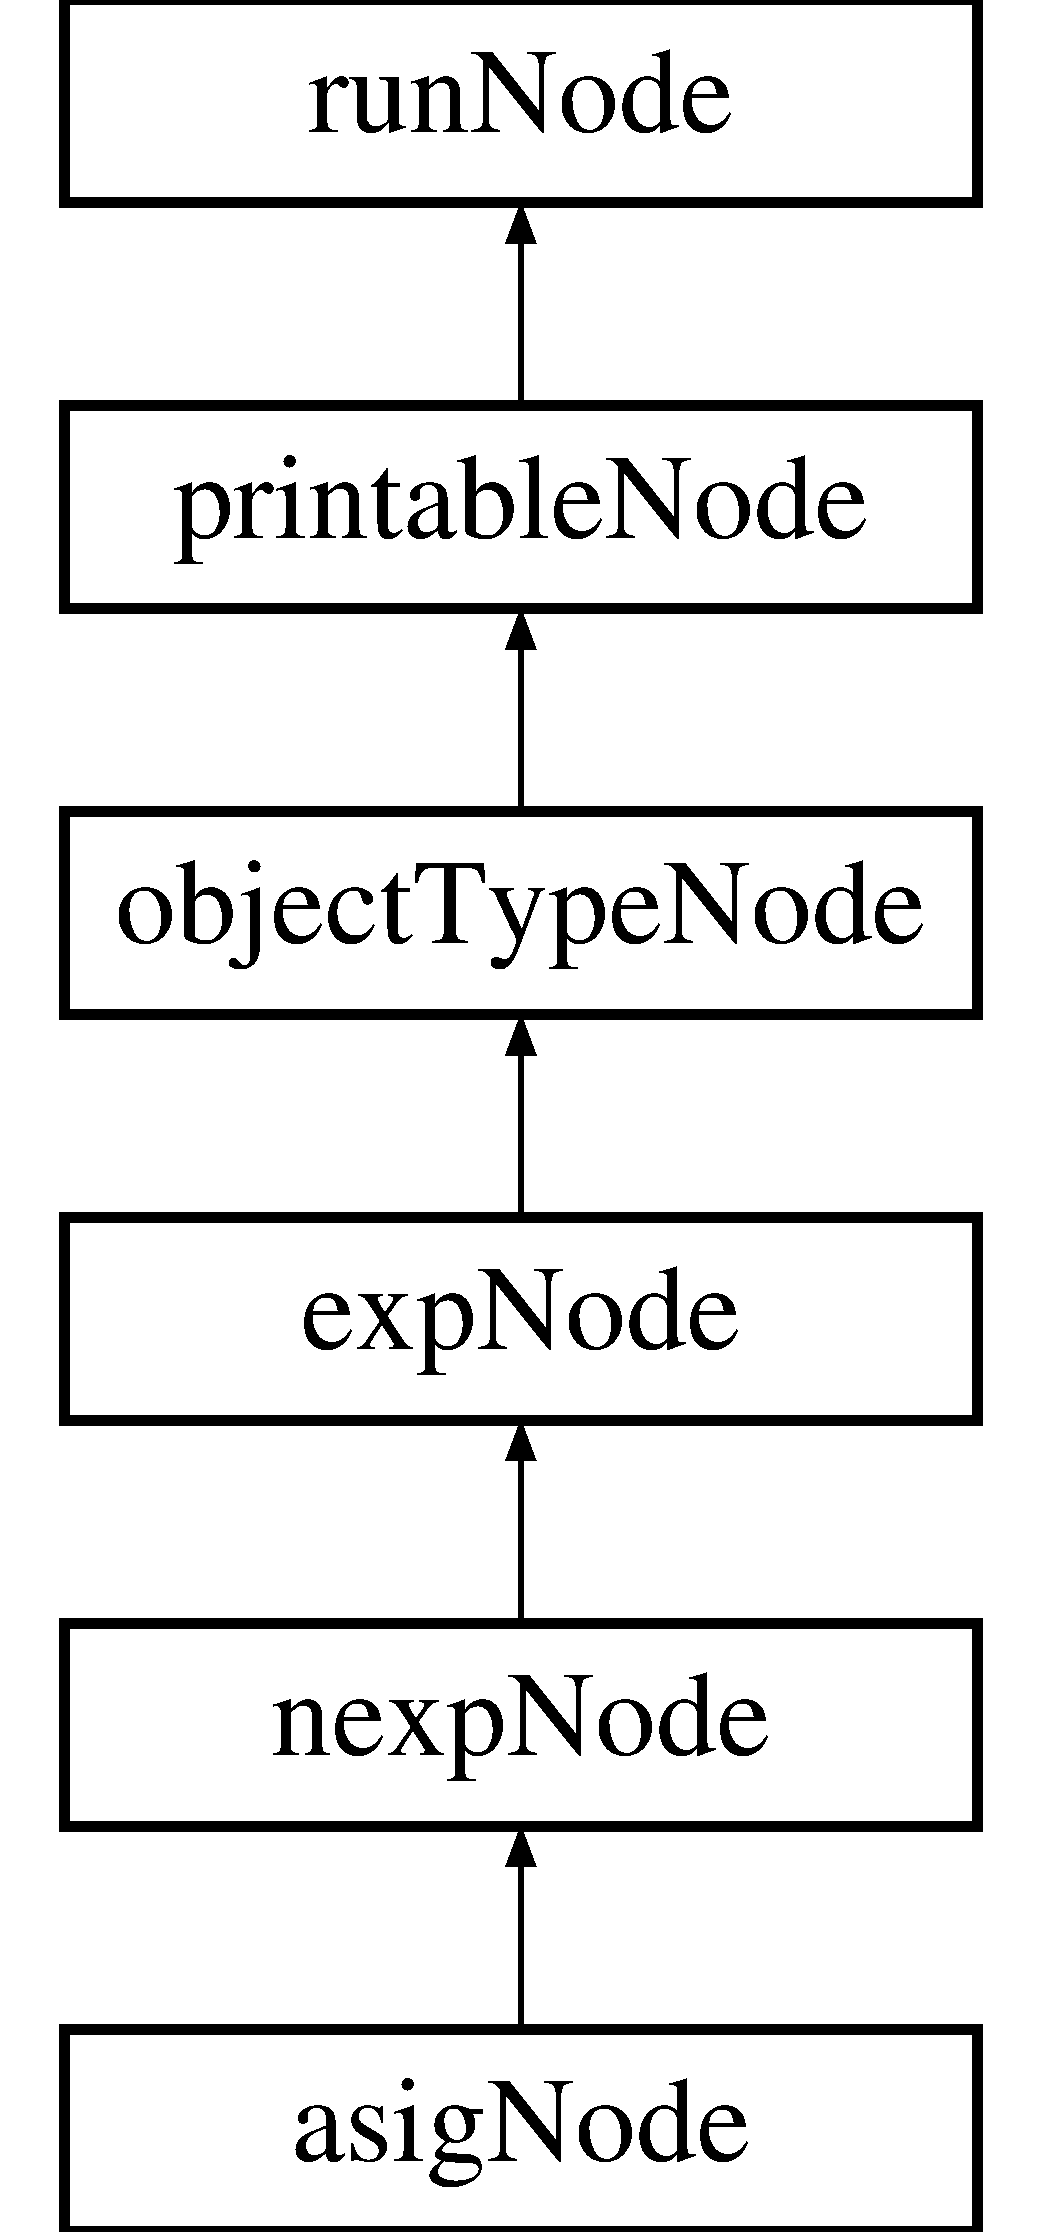
\includegraphics[height=6.000000cm]{classasigNode}
\end{center}
\end{figure}
\subsection*{Métodos públicos}
\begin{DoxyCompactItemize}
\item 
\hyperlink{classasigNode_ad8a2612519f5aa530dbdb0efe0987044}{asig\-Node} (\hyperlink{classrunNode}{run\-Node} $\ast$node1, \hyperlink{classrunNode}{run\-Node} $\ast$node2)
\item 
void \hyperlink{classasigNode_a7009318d86f9bcb728933074015fcf22}{run} ()
\item 
void \hyperlink{classasigNode_a2b95850e36d0c65e0e8bbbf2f49d106a}{run\-Level} ()
\item 
void \hyperlink{classasigNode_a5d43f5aacfd7a906a8454cb5ef55ff0a}{set\-Value} (\hyperlink{classrunNode}{run\-Node} $\ast$node)
\item 
\hyperlink{classrunNode}{run\-Node} $\ast$ \hyperlink{classasigNode_a8902a08795822d1e04f0c3a28ed8492b}{get\-Left} ()
\item 
\hyperlink{classrunNode}{run\-Node} $\ast$ \hyperlink{classasigNode_a3aff56b9b19402e286846e7eae023fba}{get\-Right} ()
\item 
bool \hyperlink{classasigNode_a36ca81966c60c93f1b8c38fce719b000}{is\-\_\-runlist} () const 
\end{DoxyCompactItemize}
\subsection*{Otros miembros heredados}


\subsection{Descripción detallada}
Nodo asignación. 

Asigna el valor de un nodo a otro. La asignación se debe realizar sobre una expresión de tipo no definido, modificándose la referencia interna de este al nodo asignado.

Si el nodo que es asignado es constante será clonado y se asignará la copia. Si el nodo es dinámico se asigna el propio nodo aumentaándose el número de referencias del mismo.

La asignación es en si misma una expresión de tipo no definido cuyo valor tras la ejecución será el nodo asignado. 

\subsection{Documentación del constructor y destructor}
\hypertarget{classasigNode_ad8a2612519f5aa530dbdb0efe0987044}{\index{asig\-Node@{asig\-Node}!asig\-Node@{asig\-Node}}
\index{asig\-Node@{asig\-Node}!asigNode@{asig\-Node}}
\subsubsection[{asig\-Node}]{\setlength{\rightskip}{0pt plus 5cm}asig\-Node\-::asig\-Node (
\begin{DoxyParamCaption}
\item[{{\bf run\-Node} $\ast$}]{node1, }
\item[{{\bf run\-Node} $\ast$}]{node2}
\end{DoxyParamCaption}
)}}\label{classasigNode_ad8a2612519f5aa530dbdb0efe0987044}
Construcutor de la clase que asocia los nodos al nodo operación de asignación 
\begin{DoxyParams}{Parámetros}
{\em node1} & Nodo sobre el que se realizará la asignación \\
\hline
{\em node2} & Nodo que será asignado \\
\hline
\end{DoxyParams}


\subsection{Documentación de las funciones miembro}
\hypertarget{classasigNode_a8902a08795822d1e04f0c3a28ed8492b}{\index{asig\-Node@{asig\-Node}!get\-Left@{get\-Left}}
\index{get\-Left@{get\-Left}!asigNode@{asig\-Node}}
\subsubsection[{get\-Left}]{\setlength{\rightskip}{0pt plus 5cm}{\bf run\-Node} $\ast$ asig\-Node\-::get\-Left (
\begin{DoxyParamCaption}
{}
\end{DoxyParamCaption}
)}}\label{classasigNode_a8902a08795822d1e04f0c3a28ed8492b}
Obtiene la parte izquierda del operador \begin{DoxyReturn}{Devuelve}
Nodo de la parte izquierda del operador 
\end{DoxyReturn}
\hypertarget{classasigNode_a3aff56b9b19402e286846e7eae023fba}{\index{asig\-Node@{asig\-Node}!get\-Right@{get\-Right}}
\index{get\-Right@{get\-Right}!asigNode@{asig\-Node}}
\subsubsection[{get\-Right}]{\setlength{\rightskip}{0pt plus 5cm}{\bf run\-Node} $\ast$ asig\-Node\-::get\-Right (
\begin{DoxyParamCaption}
{}
\end{DoxyParamCaption}
)}}\label{classasigNode_a3aff56b9b19402e286846e7eae023fba}
Obtiene la parte derecha del operador \begin{DoxyReturn}{Devuelve}
Nodo de la parte derecha del operador 
\end{DoxyReturn}
\hypertarget{classasigNode_a36ca81966c60c93f1b8c38fce719b000}{\index{asig\-Node@{asig\-Node}!is\-\_\-runlist@{is\-\_\-runlist}}
\index{is\-\_\-runlist@{is\-\_\-runlist}!asigNode@{asig\-Node}}
\subsubsection[{is\-\_\-runlist}]{\setlength{\rightskip}{0pt plus 5cm}bool asig\-Node\-::is\-\_\-runlist (
\begin{DoxyParamCaption}
{}
\end{DoxyParamCaption}
) const\hspace{0.3cm}{\ttfamily [virtual]}}}\label{classasigNode_a36ca81966c60c93f1b8c38fce719b000}
Las asignaciones deben ser ejecutadas cunado se encuentran dentro de una lista. 

Reimplementado de \hyperlink{classrunNode_a231638d0fc5b436c5e4a664fe7d5126a}{run\-Node}.

\hypertarget{classasigNode_a7009318d86f9bcb728933074015fcf22}{\index{asig\-Node@{asig\-Node}!run@{run}}
\index{run@{run}!asigNode@{asig\-Node}}
\subsubsection[{run}]{\setlength{\rightskip}{0pt plus 5cm}void asig\-Node\-::run (
\begin{DoxyParamCaption}
{}
\end{DoxyParamCaption}
)\hspace{0.3cm}{\ttfamily [virtual]}}}\label{classasigNode_a7009318d86f9bcb728933074015fcf22}
Método que ejecuta el nodo. Se lleva a cabo la asignación, para ello se procesa el lado derecho de la asignación. Luego este valor es asignado a como referencia del lado izquierdo.

Tras la ejecución se toma como valor el nodo asignado 

Implementa \hyperlink{classrunNode_a83c10df8148829b08e04153c93d69eec}{run\-Node}.

\hypertarget{classasigNode_a2b95850e36d0c65e0e8bbbf2f49d106a}{\index{asig\-Node@{asig\-Node}!run\-Level@{run\-Level}}
\index{run\-Level@{run\-Level}!asigNode@{asig\-Node}}
\subsubsection[{run\-Level}]{\setlength{\rightskip}{0pt plus 5cm}void asig\-Node\-::run\-Level (
\begin{DoxyParamCaption}
{}
\end{DoxyParamCaption}
)}}\label{classasigNode_a2b95850e36d0c65e0e8bbbf2f49d106a}
Método que ejecuta el nodo entre niveles de la tabla de símbolos. Se lleva a cabo la asignación, para ello se procesa el lado derecho de la asignación en el nivel anterior de la tabla de símbolos. Luego este valor es asignado a como referencia del lado izquierdo en el nivel actual de la tabla de símbolos.

Generalmente el lado izquierdo de la expresión será un identificador.

Tras la ejecución se toma como valor el nodo asignado \hypertarget{classasigNode_a5d43f5aacfd7a906a8454cb5ef55ff0a}{\index{asig\-Node@{asig\-Node}!set\-Value@{set\-Value}}
\index{set\-Value@{set\-Value}!asigNode@{asig\-Node}}
\subsubsection[{set\-Value}]{\setlength{\rightskip}{0pt plus 5cm}void asig\-Node\-::set\-Value (
\begin{DoxyParamCaption}
\item[{{\bf run\-Node} $\ast$}]{node}
\end{DoxyParamCaption}
)}}\label{classasigNode_a5d43f5aacfd7a906a8454cb5ef55ff0a}
Asigna el valor de un nodo dado al referencia del nodo del lado izquierdo del operador 

La documentación para esta clase fue generada a partir de los siguientes ficheros\-:\begin{DoxyCompactItemize}
\item 
trunk/src/run/operators/\hyperlink{symbolOpNode_8h}{symbol\-Op\-Node.\-h}\item 
trunk/src/run/operators/symbol\-Op\-Node.\-cpp\end{DoxyCompactItemize}

\hypertarget{classasigrefNode}{\section{Referencia de la Clase asigref\-Node}
\label{classasigrefNode}\index{asigref\-Node@{asigref\-Node}}
}


Nodo asignación.  




{\ttfamily \#include $<$symbol\-Op\-Node.\-h$>$}

Diagrama de herencias de asigref\-Node\begin{figure}[H]
\begin{center}
\leavevmode
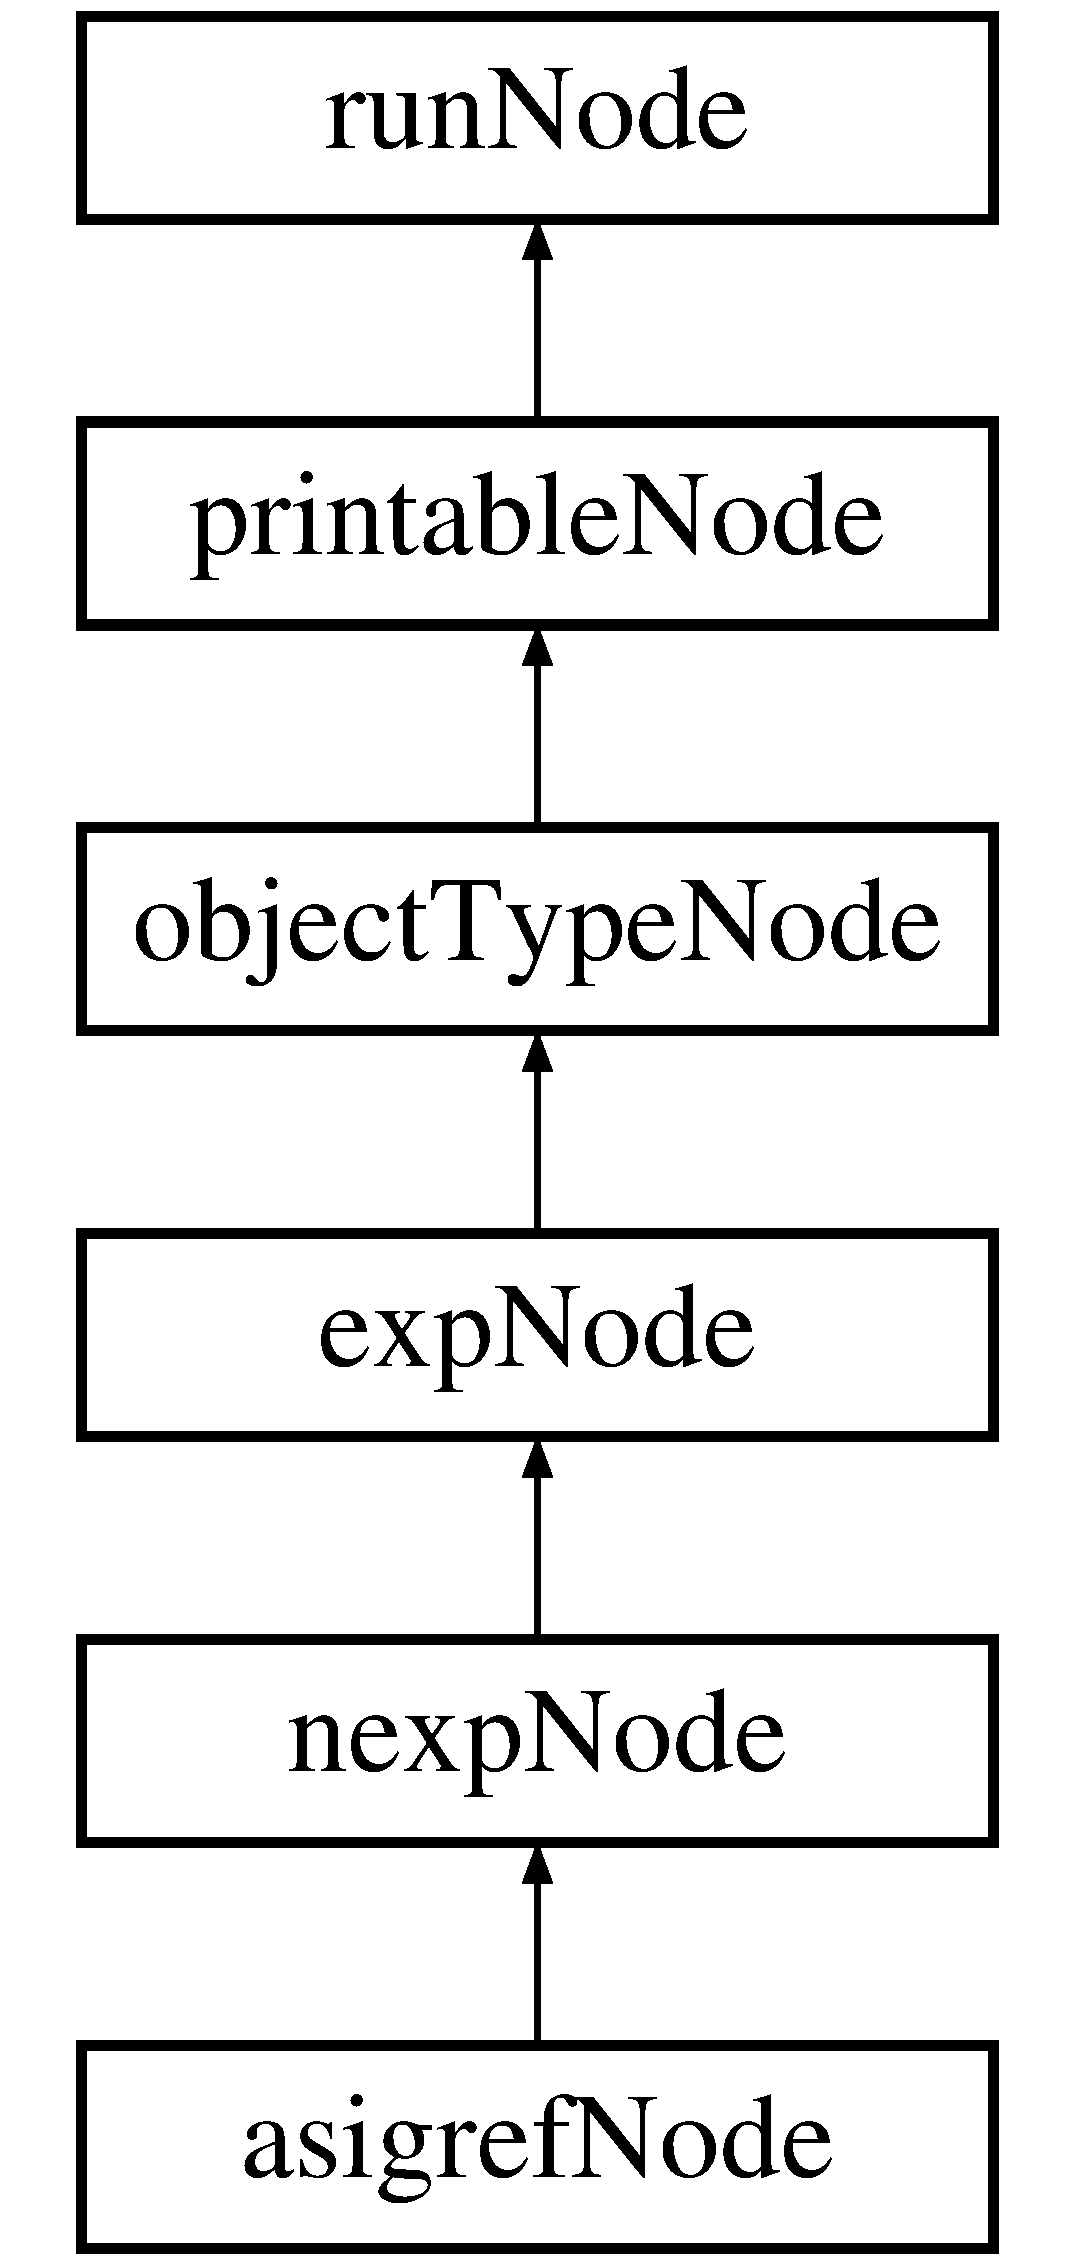
\includegraphics[height=6.000000cm]{classasigrefNode}
\end{center}
\end{figure}
\subsection*{Métodos públicos}
\begin{DoxyCompactItemize}
\item 
\hyperlink{classasigrefNode_a817c24e32d9c8d28298172ffe97978ba}{asigref\-Node} (\hyperlink{classrunNode}{run\-Node} $\ast$node1, \hyperlink{classrunNode}{run\-Node} $\ast$node2)
\item 
void \hyperlink{classasigrefNode_a208e32830e6f43157a94d993c599ed00}{run} ()
\item 
void \hyperlink{classasigrefNode_ae88032a024d5e5033b53cac65f14b0c4}{set\-Value} (\hyperlink{classrunNode}{run\-Node} $\ast$node)
\end{DoxyCompactItemize}
\subsection*{Otros miembros heredados}


\subsection{Descripción detallada}
Nodo asignación. 

Este nodo es utilizado en las listas de parámetros e indica que un parámetro debe ser pasado por referencia.

Al ejecutarse se asigna una referencia al nodo. 

\subsection{Documentación del constructor y destructor}
\hypertarget{classasigrefNode_a817c24e32d9c8d28298172ffe97978ba}{\index{asigref\-Node@{asigref\-Node}!asigref\-Node@{asigref\-Node}}
\index{asigref\-Node@{asigref\-Node}!asigrefNode@{asigref\-Node}}
\subsubsection[{asigref\-Node}]{\setlength{\rightskip}{0pt plus 5cm}asigref\-Node\-::asigref\-Node (
\begin{DoxyParamCaption}
\item[{{\bf run\-Node} $\ast$}]{node1, }
\item[{{\bf run\-Node} $\ast$}]{node2}
\end{DoxyParamCaption}
)}}\label{classasigrefNode_a817c24e32d9c8d28298172ffe97978ba}
Construcutor de la clase que asocia los nodos al nodo operación de asignación de referencia. 
\begin{DoxyParams}{Parámetros}
{\em node1} & Nodo sobre el que se realizará la asignación \\
\hline
{\em node2} & Nodo que será asignado \\
\hline
\end{DoxyParams}


\subsection{Documentación de las funciones miembro}
\hypertarget{classasigrefNode_a208e32830e6f43157a94d993c599ed00}{\index{asigref\-Node@{asigref\-Node}!run@{run}}
\index{run@{run}!asigrefNode@{asigref\-Node}}
\subsubsection[{run}]{\setlength{\rightskip}{0pt plus 5cm}void asigref\-Node\-::run (
\begin{DoxyParamCaption}
{}
\end{DoxyParamCaption}
)\hspace{0.3cm}{\ttfamily [virtual]}}}\label{classasigrefNode_a208e32830e6f43157a94d993c599ed00}
Método que ejecuta el nodo. Se lleva a cabo la asignación, para ello se procesa el lado derecho de la asignación, se obtiene una referencia al mismo como valor interno. Luego este valor es asignado como referencia del lado izquierdo. 

Implementa \hyperlink{classrunNode_a83c10df8148829b08e04153c93d69eec}{run\-Node}.

\hypertarget{classasigrefNode_ae88032a024d5e5033b53cac65f14b0c4}{\index{asigref\-Node@{asigref\-Node}!set\-Value@{set\-Value}}
\index{set\-Value@{set\-Value}!asigrefNode@{asigref\-Node}}
\subsubsection[{set\-Value}]{\setlength{\rightskip}{0pt plus 5cm}void asigref\-Node\-::set\-Value (
\begin{DoxyParamCaption}
\item[{{\bf run\-Node} $\ast$}]{node}
\end{DoxyParamCaption}
)}}\label{classasigrefNode_ae88032a024d5e5033b53cac65f14b0c4}
Asigna el valor de un nodo dado al referencia del nodo del lado izquierdo del operador 

La documentación para esta clase fue generada a partir de los siguientes ficheros\-:\begin{DoxyCompactItemize}
\item 
trunk/src/run/operators/\hyperlink{symbolOpNode_8h}{symbol\-Op\-Node.\-h}\item 
trunk/src/run/operators/symbol\-Op\-Node.\-cpp\end{DoxyCompactItemize}

\hypertarget{classboolConstNode}{\section{Referencia de la Clase bool\-Const\-Node}
\label{classboolConstNode}\index{bool\-Const\-Node@{bool\-Const\-Node}}
}


Nodo boleano constante.  




{\ttfamily \#include $<$type\-Node.\-h$>$}

Diagrama de herencias de bool\-Const\-Node\begin{figure}[H]
\begin{center}
\leavevmode
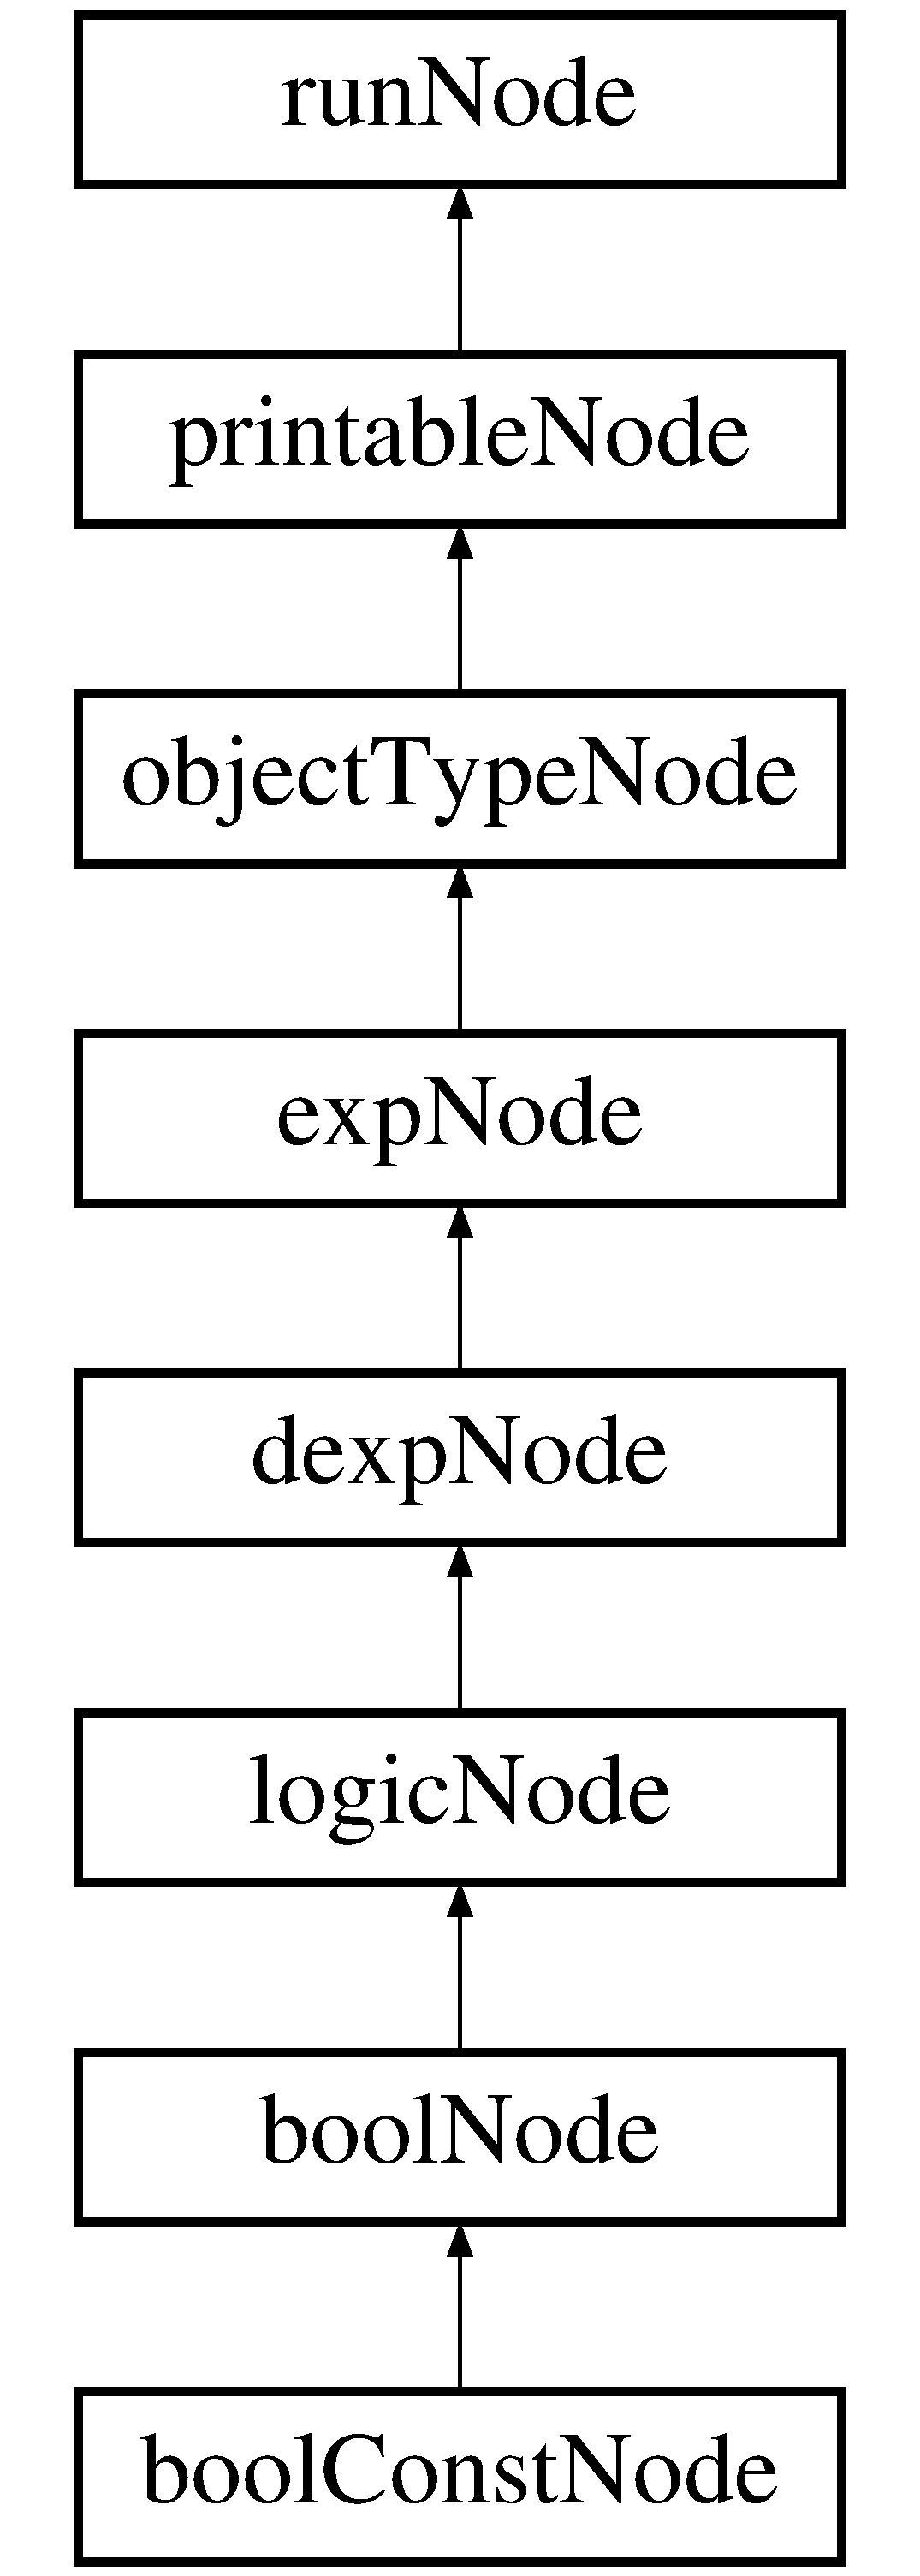
\includegraphics[height=8.000000cm]{classboolConstNode}
\end{center}
\end{figure}
\subsection*{Métodos públicos}
\begin{DoxyCompactItemize}
\item 
\hyperlink{classboolConstNode_aabc766d61745b2816061f803cb5520a4}{bool\-Const\-Node} (bool data)
\item 
void \hyperlink{classboolConstNode_a2f87a46feab71dc6f3fab0be3023a1cf}{rm\-Ref} ()
\end{DoxyCompactItemize}
\subsection*{Otros miembros heredados}


\subsection{Descripción detallada}
Nodo boleano constante. 

Un nodo constante sobrecarga el método de eliminar referencia para que no pueda ser eliminado de la forma normal. 

\subsection{Documentación del constructor y destructor}
\hypertarget{classboolConstNode_aabc766d61745b2816061f803cb5520a4}{\index{bool\-Const\-Node@{bool\-Const\-Node}!bool\-Const\-Node@{bool\-Const\-Node}}
\index{bool\-Const\-Node@{bool\-Const\-Node}!boolConstNode@{bool\-Const\-Node}}
\subsubsection[{bool\-Const\-Node}]{\setlength{\rightskip}{0pt plus 5cm}bool\-Const\-Node\-::bool\-Const\-Node (
\begin{DoxyParamCaption}
\item[{bool}]{data}
\end{DoxyParamCaption}
)}}\label{classboolConstNode_aabc766d61745b2816061f803cb5520a4}
Constructor de la clase. 
\begin{DoxyParams}{Parámetros}
{\em data} & Valor booleano del nodo. \\
\hline
\end{DoxyParams}


\subsection{Documentación de las funciones miembro}
\hypertarget{classboolConstNode_a2f87a46feab71dc6f3fab0be3023a1cf}{\index{bool\-Const\-Node@{bool\-Const\-Node}!rm\-Ref@{rm\-Ref}}
\index{rm\-Ref@{rm\-Ref}!boolConstNode@{bool\-Const\-Node}}
\subsubsection[{rm\-Ref}]{\setlength{\rightskip}{0pt plus 5cm}void bool\-Const\-Node\-::rm\-Ref (
\begin{DoxyParamCaption}
{}
\end{DoxyParamCaption}
)\hspace{0.3cm}{\ttfamily [virtual]}}}\label{classboolConstNode_a2f87a46feab71dc6f3fab0be3023a1cf}
Sobrecarga del método para eliminar referencias. 

Reimplementado de \hyperlink{classrunNode_a8d0761660753ceb2c98836614c526a45}{run\-Node}.



La documentación para esta clase fue generada a partir de los siguientes ficheros\-:\begin{DoxyCompactItemize}
\item 
trunk/src/run/tree/\hyperlink{typeNode_8h}{type\-Node.\-h}\item 
trunk/src/run/tree/\hyperlink{typeNode_8cpp}{type\-Node.\-cpp}\end{DoxyCompactItemize}

\hypertarget{classboolconvNode}{\section{Referencia de la Clase boolconv\-Node}
\label{classboolconvNode}\index{boolconv\-Node@{boolconv\-Node}}
}


Nodo de conversión a booleano.  




{\ttfamily \#include $<$conv\-Op\-Node.\-h$>$}

Diagrama de herencias de boolconv\-Node\begin{figure}[H]
\begin{center}
\leavevmode
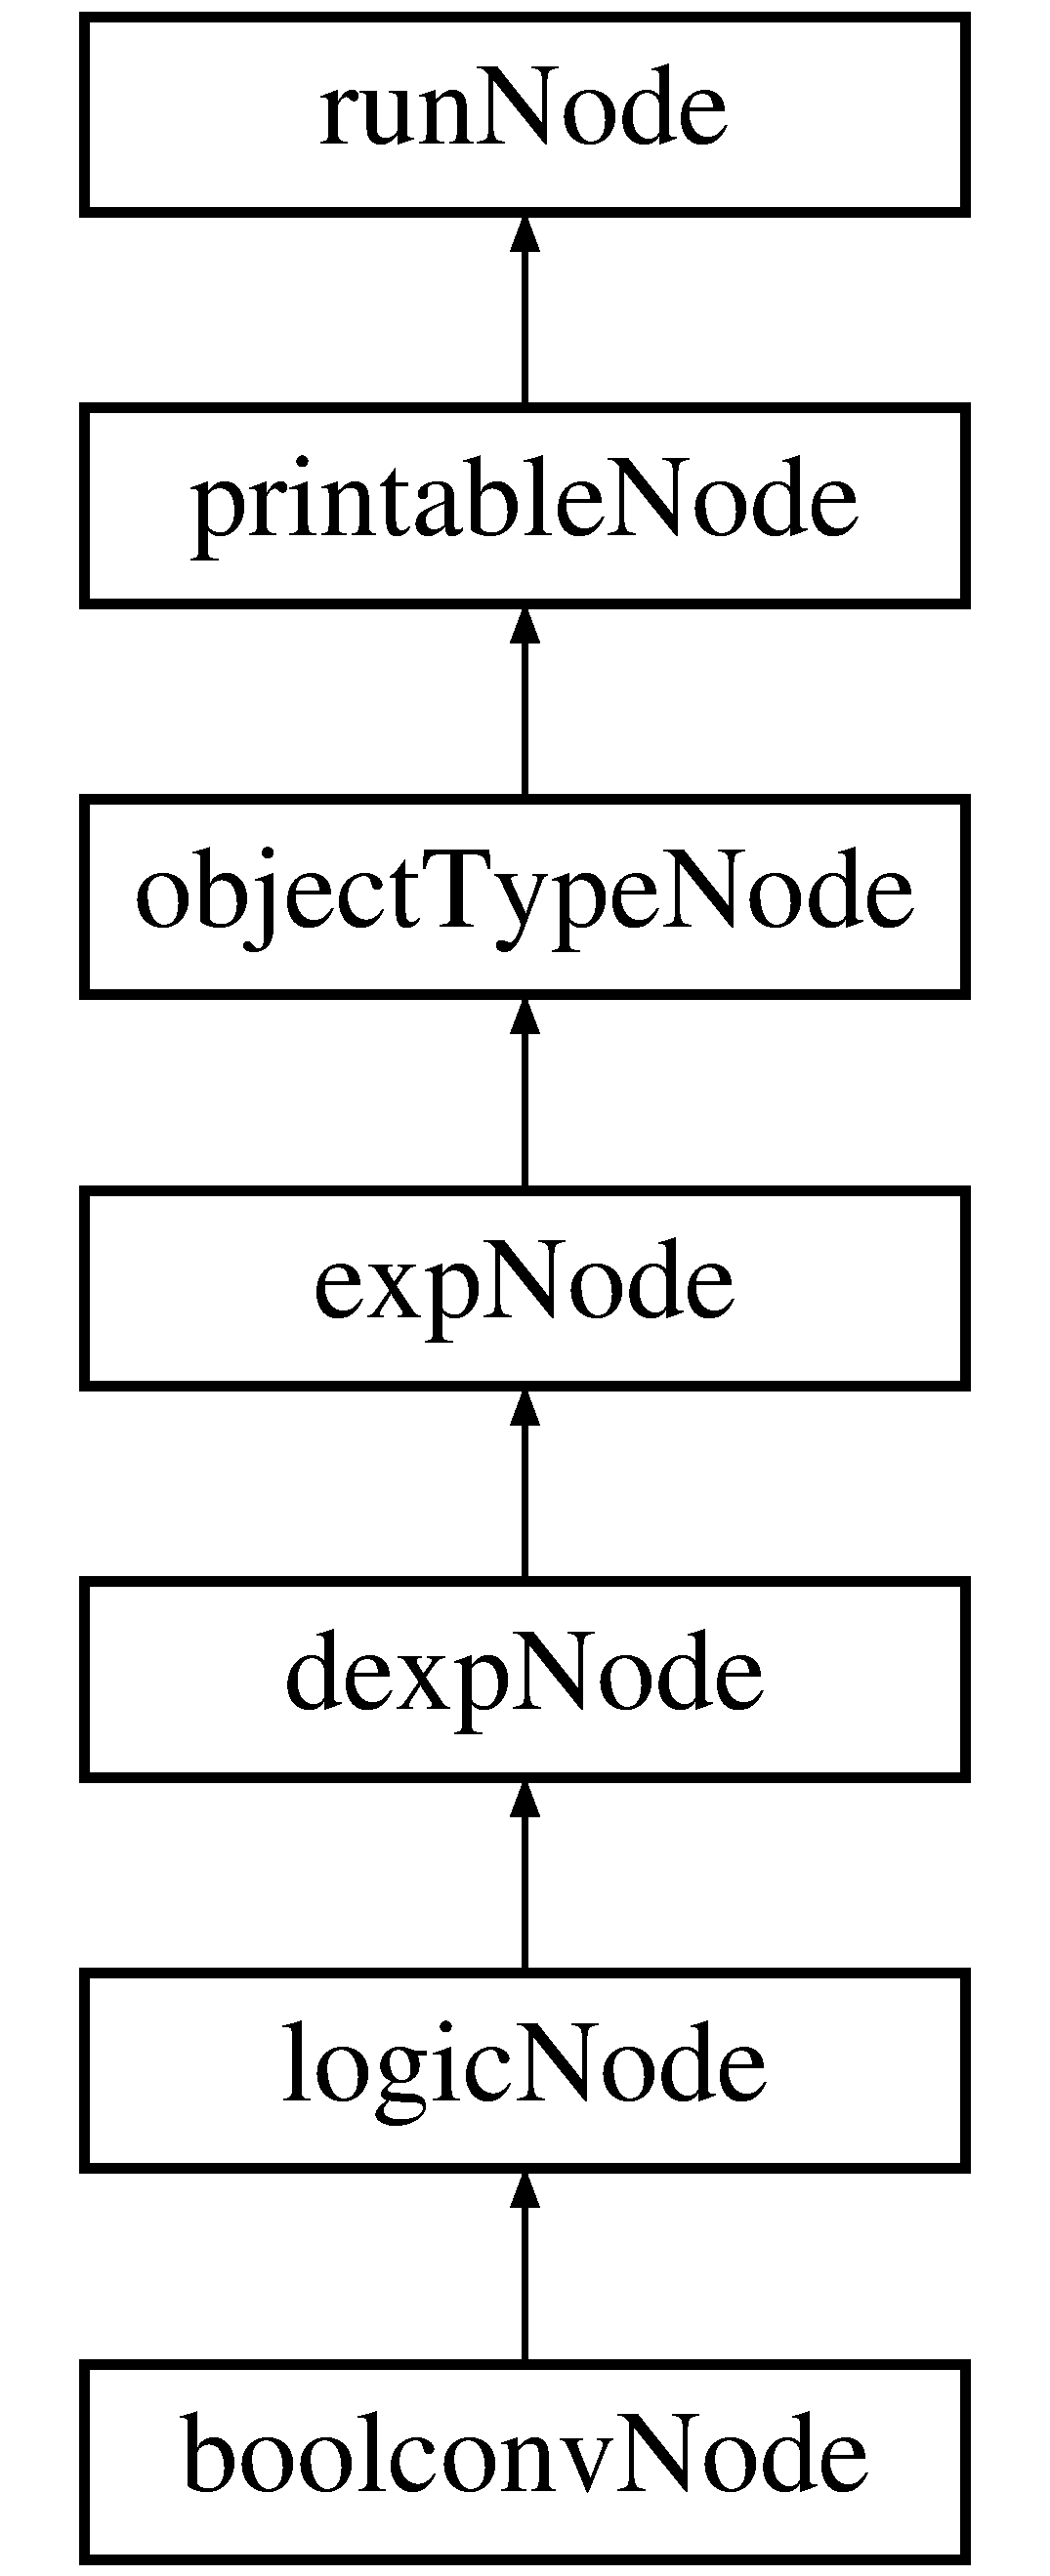
\includegraphics[height=7.000000cm]{classboolconvNode}
\end{center}
\end{figure}
\subsection*{Métodos públicos}
\begin{DoxyCompactItemize}
\item 
\hyperlink{classboolconvNode_a5e675df17489517475859bc393f232ce}{boolconv\-Node} (\hyperlink{classrunNode}{run\-Node} $\ast$node)
\item 
void \hyperlink{classboolconvNode_a344001e8903f5969a0187021d749c637}{run} ()
\end{DoxyCompactItemize}
\subsection*{Métodos públicos estáticos}
\begin{DoxyCompactItemize}
\item 
static num \hyperlink{classboolconvNode_a7bb697f6a097e580cb5fbfb1c0b6391a}{do\-\_\-boolconv} (\hyperlink{classrunNode}{run\-Node} $\ast$node)
\end{DoxyCompactItemize}
\subsection*{Otros miembros heredados}


\subsection{Descripción detallada}
Nodo de conversión a booleano. 

Este nodo fuerza la conversion a booleano del valor de un nodo

Si el nodo es booleano toma su propio valor Si el nodo es aritmético toma el valor booleano del nodo Si el nodo es cadena de texto toma verdadero si la cadena no es vacia Si el nodo es array toma verdadero si el array no está vacio 

\subsection{Documentación del constructor y destructor}
\hypertarget{classboolconvNode_a5e675df17489517475859bc393f232ce}{\index{boolconv\-Node@{boolconv\-Node}!boolconv\-Node@{boolconv\-Node}}
\index{boolconv\-Node@{boolconv\-Node}!boolconvNode@{boolconv\-Node}}
\subsubsection[{boolconv\-Node}]{\setlength{\rightskip}{0pt plus 5cm}boolconv\-Node\-::boolconv\-Node (
\begin{DoxyParamCaption}
\item[{{\bf run\-Node} $\ast$}]{node}
\end{DoxyParamCaption}
)}}\label{classboolconvNode_a5e675df17489517475859bc393f232ce}
Constructor de la clase. Asocia el nodo operador a un nodo. 
\begin{DoxyParams}{Parámetros}
{\em node} & Nodo operando. \\
\hline
\end{DoxyParams}


\subsection{Documentación de las funciones miembro}
\hypertarget{classboolconvNode_a7bb697f6a097e580cb5fbfb1c0b6391a}{\index{boolconv\-Node@{boolconv\-Node}!do\-\_\-boolconv@{do\-\_\-boolconv}}
\index{do\-\_\-boolconv@{do\-\_\-boolconv}!boolconvNode@{boolconv\-Node}}
\subsubsection[{do\-\_\-boolconv}]{\setlength{\rightskip}{0pt plus 5cm}num boolconv\-Node\-::do\-\_\-boolconv (
\begin{DoxyParamCaption}
\item[{{\bf run\-Node} $\ast$}]{node}
\end{DoxyParamCaption}
)\hspace{0.3cm}{\ttfamily [static]}}}\label{classboolconvNode_a7bb697f6a097e580cb5fbfb1c0b6391a}
Convierte un nodo a su valor booleano 
\begin{DoxyParams}{Parámetros}
{\em node} & Nodo operando. \\
\hline
\end{DoxyParams}
\begin{DoxyReturn}{Devuelve}
Valor de la operación 
\end{DoxyReturn}
\hypertarget{classboolconvNode_a344001e8903f5969a0187021d749c637}{\index{boolconv\-Node@{boolconv\-Node}!run@{run}}
\index{run@{run}!boolconvNode@{boolconv\-Node}}
\subsubsection[{run}]{\setlength{\rightskip}{0pt plus 5cm}void boolconv\-Node\-::run (
\begin{DoxyParamCaption}
{}
\end{DoxyParamCaption}
)\hspace{0.3cm}{\ttfamily [virtual]}}}\label{classboolconvNode_a344001e8903f5969a0187021d749c637}
Tras ser ejecutado el operador toma como valor el resultado de la conversión a booleano del nodo asociado 

Implementa \hyperlink{classrunNode_a83c10df8148829b08e04153c93d69eec}{run\-Node}.



La documentación para esta clase fue generada a partir de los siguientes ficheros\-:\begin{DoxyCompactItemize}
\item 
trunk/src/run/operators/\hyperlink{convOpNode_8h}{conv\-Op\-Node.\-h}\item 
trunk/src/run/operators/conv\-Op\-Node.\-cpp\end{DoxyCompactItemize}

\hypertarget{classboolNode}{\section{Referencia de la Clase bool\-Node}
\label{classboolNode}\index{bool\-Node@{bool\-Node}}
}


Nodo booleano.  




{\ttfamily \#include $<$type\-Node.\-h$>$}

Diagrama de herencias de bool\-Node\begin{figure}[H]
\begin{center}
\leavevmode
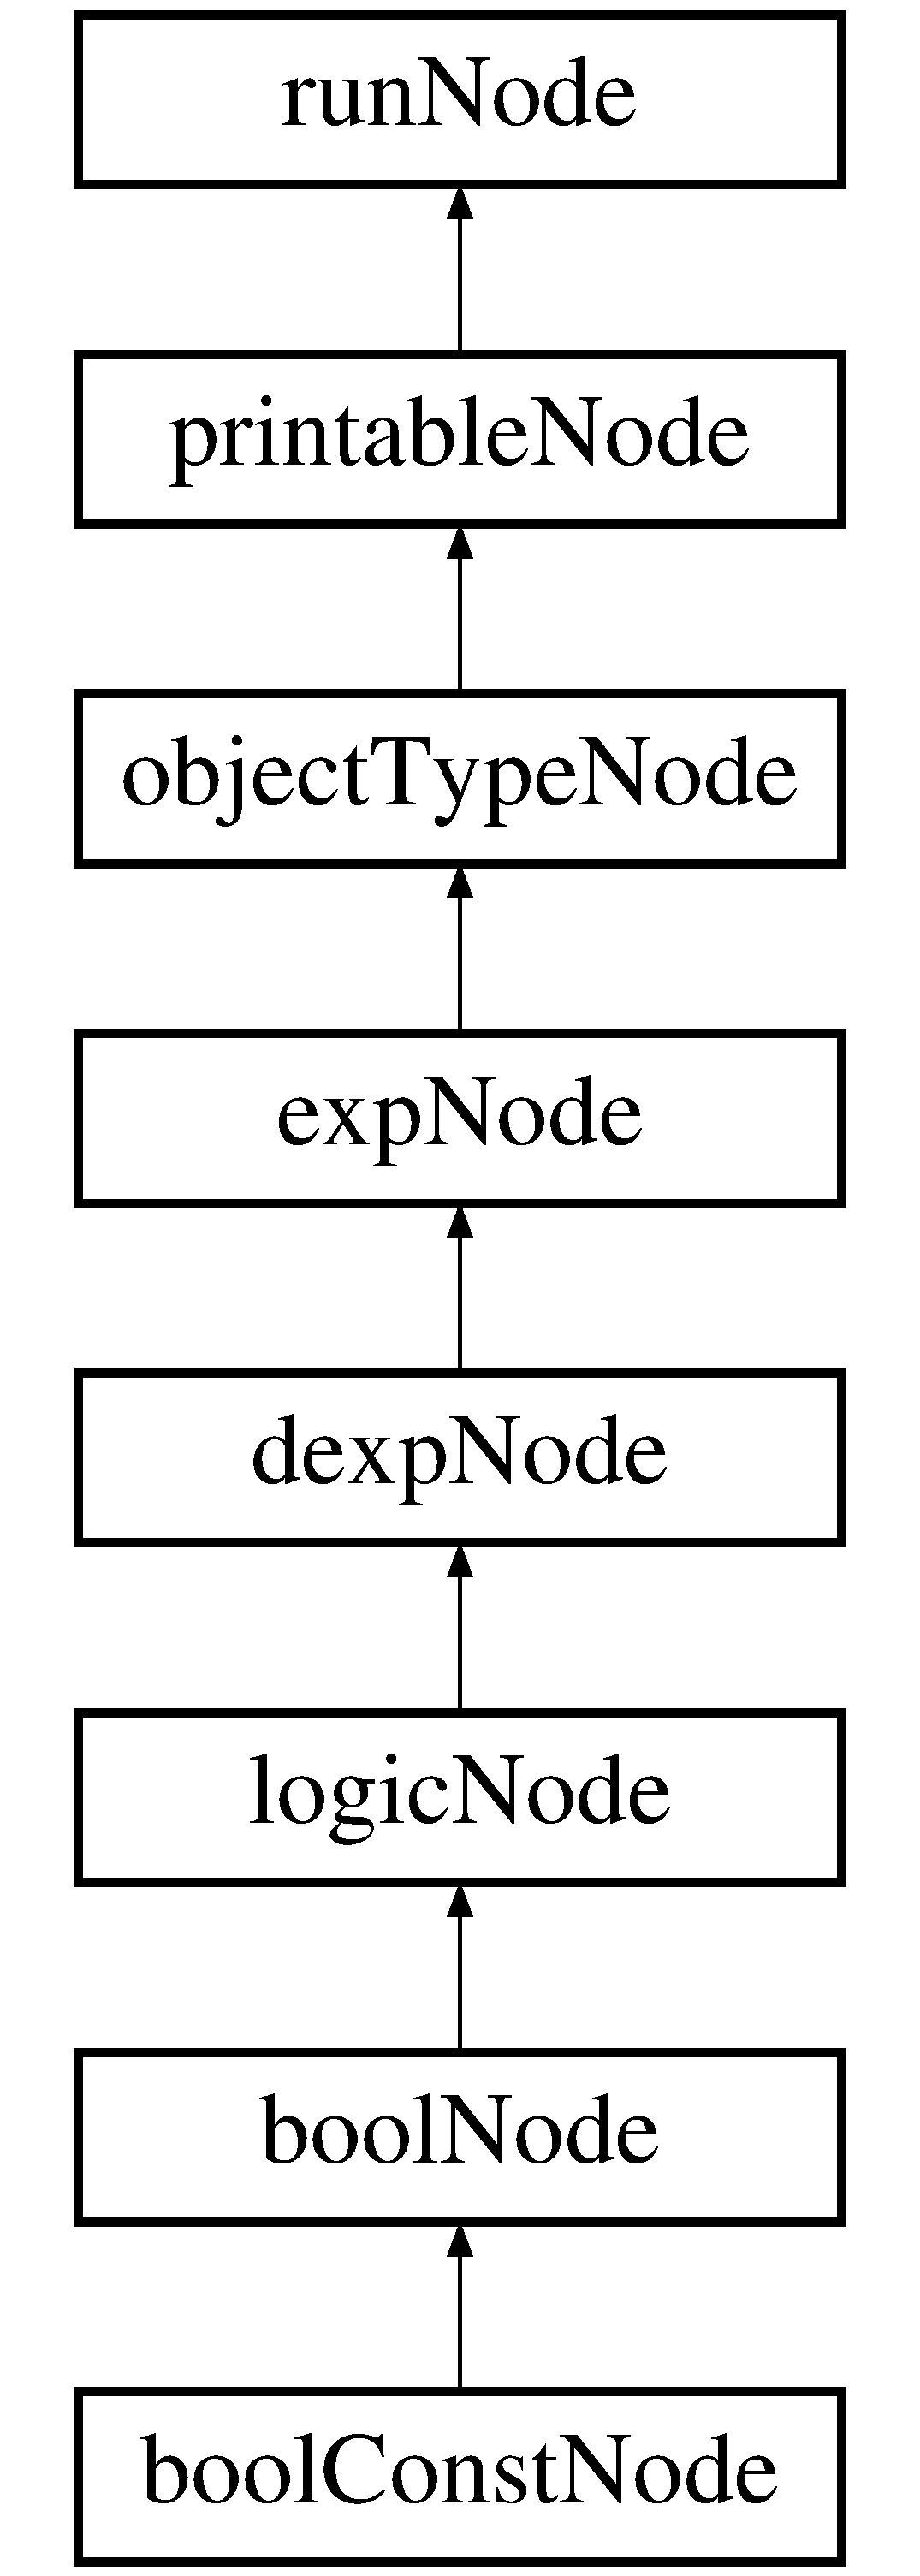
\includegraphics[height=8.000000cm]{classboolNode}
\end{center}
\end{figure}
\subsection*{Métodos públicos}
\begin{DoxyCompactItemize}
\item 
\hyperlink{classboolNode_a524ead471357541fbd134467f831e414}{bool\-Node} (bool data)
\item 
\hyperlink{classboolNode_af8d6de46de3631dfd1d9ae131dab374e}{bool\-Node} (\hyperlink{classboolNode}{bool\-Node} $\ast$data)
\item 
void \hyperlink{classboolNode_a98c7446189867e474cd759334b30a9ad}{run} ()
\end{DoxyCompactItemize}
\subsection*{Otros miembros heredados}


\subsection{Descripción detallada}
Nodo booleano. 

Representa un dato booleano, \char`\"{}true\char`\"{} o \char`\"{}false\char`\"{}. 

\subsection{Documentación del constructor y destructor}
\hypertarget{classboolNode_a524ead471357541fbd134467f831e414}{\index{bool\-Node@{bool\-Node}!bool\-Node@{bool\-Node}}
\index{bool\-Node@{bool\-Node}!boolNode@{bool\-Node}}
\subsubsection[{bool\-Node}]{\setlength{\rightskip}{0pt plus 5cm}bool\-Node\-::bool\-Node (
\begin{DoxyParamCaption}
\item[{bool}]{data}
\end{DoxyParamCaption}
)}}\label{classboolNode_a524ead471357541fbd134467f831e414}
Constructor que asigna el valor del nodo. 
\begin{DoxyParams}{Parámetros}
{\em data} & Dato booleano. \\
\hline
\end{DoxyParams}
\hypertarget{classboolNode_af8d6de46de3631dfd1d9ae131dab374e}{\index{bool\-Node@{bool\-Node}!bool\-Node@{bool\-Node}}
\index{bool\-Node@{bool\-Node}!boolNode@{bool\-Node}}
\subsubsection[{bool\-Node}]{\setlength{\rightskip}{0pt plus 5cm}bool\-Node\-::bool\-Node (
\begin{DoxyParamCaption}
\item[{{\bf bool\-Node} $\ast$}]{data}
\end{DoxyParamCaption}
)}}\label{classboolNode_af8d6de46de3631dfd1d9ae131dab374e}
Constructor de copia. 
\begin{DoxyParams}{Parámetros}
{\em data} & Nodo booleano. \\
\hline
\end{DoxyParams}


\subsection{Documentación de las funciones miembro}
\hypertarget{classboolNode_a98c7446189867e474cd759334b30a9ad}{\index{bool\-Node@{bool\-Node}!run@{run}}
\index{run@{run}!boolNode@{bool\-Node}}
\subsubsection[{run}]{\setlength{\rightskip}{0pt plus 5cm}void bool\-Node\-::run (
\begin{DoxyParamCaption}
{}
\end{DoxyParamCaption}
)\hspace{0.3cm}{\ttfamily [virtual]}}}\label{classboolNode_a98c7446189867e474cd759334b30a9ad}
Función de ejecución vacía.

Esta función no realiza ninguna acción ya que el valor del nodo es asignado en la construcción. 

Implementa \hyperlink{classrunNode_a83c10df8148829b08e04153c93d69eec}{run\-Node}.



La documentación para esta clase fue generada a partir de los siguientes ficheros\-:\begin{DoxyCompactItemize}
\item 
trunk/src/run/tree/\hyperlink{typeNode_8h}{type\-Node.\-h}\item 
trunk/src/run/tree/\hyperlink{typeNode_8cpp}{type\-Node.\-cpp}\end{DoxyCompactItemize}

\hypertarget{classbreakException}{\section{Referencia de la Clase break\-Exception}
\label{classbreakException}\index{break\-Exception@{break\-Exception}}
}


Excepción rotura de bloque.  




{\ttfamily \#include $<$stmt\-Node.\-h$>$}



Herencias exception.

\subsection*{Métodos públicos}
\begin{DoxyCompactItemize}
\item 
\hyperlink{classbreakException_ac8ffef90b3602f1216eb7190cf22dc99}{break\-Exception} (int n=1)
\item 
const char $\ast$ \hyperlink{classbreakException_a46afaa17ba9edbbcc504f5caa332d8c9}{what} () const   throw ()
\item 
void \hyperlink{classbreakException_ab150b42075ee785ed64fea526b107cde}{end} ()
\end{DoxyCompactItemize}


\subsection{Descripción detallada}
Excepción rotura de bloque. 

Dados un bloque de sentencias este nodo permite romper la secuencia de ejecución hasta la salida del bloque. Esta excepción es lanzada por la sentencia break (\begin{DoxySeeAlso}{Ver también}
\hyperlink{classbreakNode}{break\-Node}). 
\end{DoxySeeAlso}


\subsection{Documentación del constructor y destructor}
\hypertarget{classbreakException_ac8ffef90b3602f1216eb7190cf22dc99}{\index{break\-Exception@{break\-Exception}!break\-Exception@{break\-Exception}}
\index{break\-Exception@{break\-Exception}!breakException@{break\-Exception}}
\subsubsection[{break\-Exception}]{\setlength{\rightskip}{0pt plus 5cm}break\-Exception\-::break\-Exception (
\begin{DoxyParamCaption}
\item[{int}]{n = {\ttfamily 1}}
\end{DoxyParamCaption}
)}}\label{classbreakException_ac8ffef90b3602f1216eb7190cf22dc99}
Constructor de la clase. 
\begin{DoxyParams}{Parámetros}
{\em init.} & Número de bloques anidados de los que se saldrá. \\
\hline
\end{DoxyParams}


\subsection{Documentación de las funciones miembro}
\hypertarget{classbreakException_ab150b42075ee785ed64fea526b107cde}{\index{break\-Exception@{break\-Exception}!end@{end}}
\index{end@{end}!breakException@{break\-Exception}}
\subsubsection[{end}]{\setlength{\rightskip}{0pt plus 5cm}void break\-Exception\-::end (
\begin{DoxyParamCaption}
{}
\end{DoxyParamCaption}
)}}\label{classbreakException_ab150b42075ee785ed64fea526b107cde}
Si el número de boloques anidados es mayor que uno lanza una excepción break decrementando el número de bloques anidados, \hypertarget{classbreakException_a46afaa17ba9edbbcc504f5caa332d8c9}{\index{break\-Exception@{break\-Exception}!what@{what}}
\index{what@{what}!breakException@{break\-Exception}}
\subsubsection[{what}]{\setlength{\rightskip}{0pt plus 5cm}const char $\ast$ break\-Exception\-::what (
\begin{DoxyParamCaption}
{}
\end{DoxyParamCaption}
) const throw  ) }}\label{classbreakException_a46afaa17ba9edbbcc504f5caa332d8c9}
Método que será llamado cuando no se capture la función, esta situación se dará cuando se produzca una sentencia break fuera de un bloque de sentencias. 

La documentación para esta clase fue generada a partir de los siguientes ficheros\-:\begin{DoxyCompactItemize}
\item 
trunk/src/run/stmts/\hyperlink{stmtNode_8h}{stmt\-Node.\-h}\item 
trunk/src/run/stmts/stmt\-Node.\-cpp\end{DoxyCompactItemize}

\hypertarget{classbreakNode}{\section{Referencia de la Clase break\-Node}
\label{classbreakNode}\index{break\-Node@{break\-Node}}
}


Nodo sentencia rotura de bloque.  




{\ttfamily \#include $<$stmt\-Node.\-h$>$}

Diagrama de herencias de break\-Node\begin{figure}[H]
\begin{center}
\leavevmode
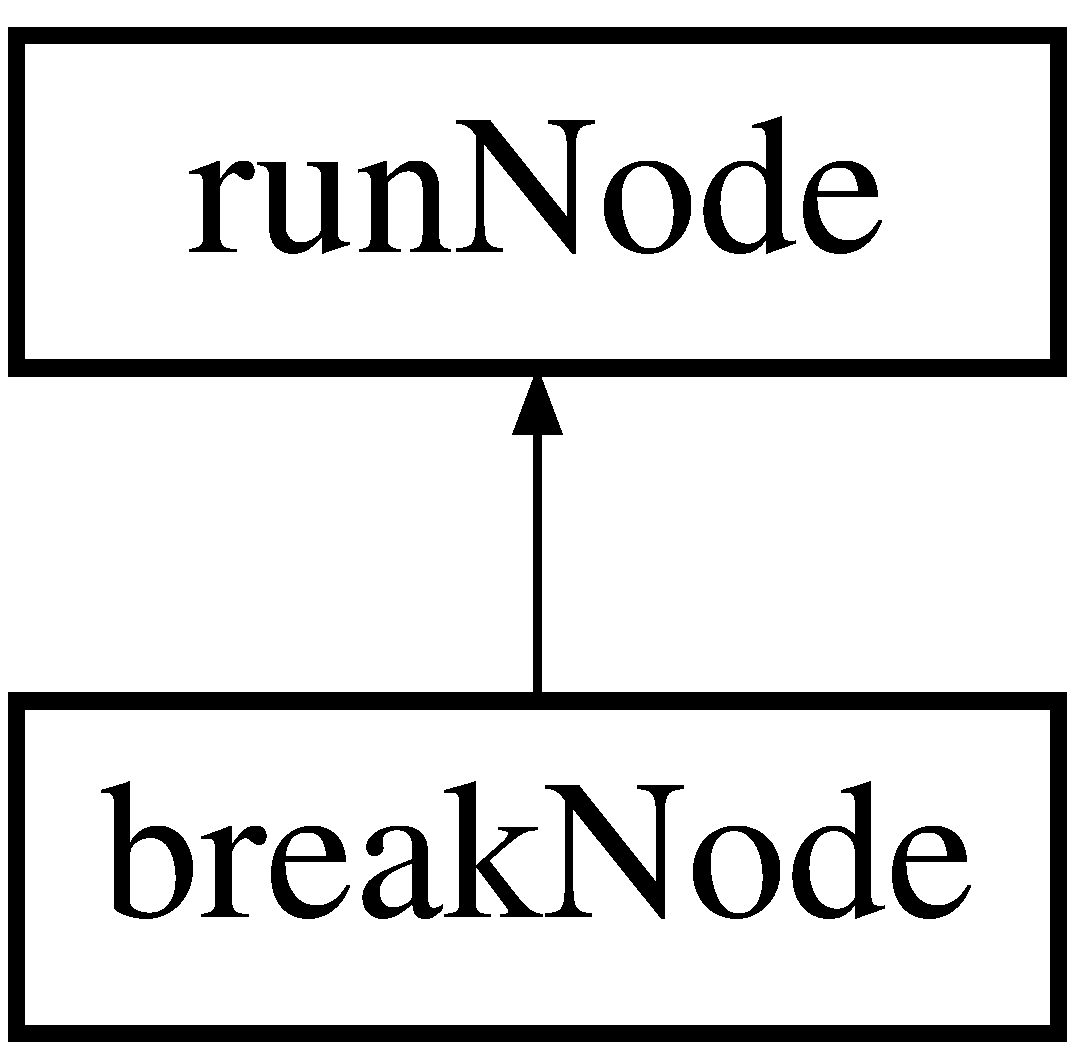
\includegraphics[height=2.000000cm]{classbreakNode}
\end{center}
\end{figure}
\subsection*{Métodos públicos}
\begin{DoxyCompactItemize}
\item 
\hyperlink{classbreakNode_a59baec750674d27ecd07a6361deaa77d}{break\-Node} (int n=1)
\item 
void \hyperlink{classbreakNode_a3fb64fa2dbc0a81922690ad041a40467}{run} ()
\end{DoxyCompactItemize}
\subsection*{Otros miembros heredados}


\subsection{Descripción detallada}
Nodo sentencia rotura de bloque. 

Este nodo representa una sentencia break, la cual consiste en finalizar la secuencia de sentencias en un bloque de estas, siguiendo en la siguiente sentencia del bloque. Adicionalmente se puede especificar el número de bloques anidados de los que se desea salir.

Si se utiliza la sentencia break fuera de un bloque de sentencias se produce un error. 

\subsection{Documentación del constructor y destructor}
\hypertarget{classbreakNode_a59baec750674d27ecd07a6361deaa77d}{\index{break\-Node@{break\-Node}!break\-Node@{break\-Node}}
\index{break\-Node@{break\-Node}!breakNode@{break\-Node}}
\subsubsection[{break\-Node}]{\setlength{\rightskip}{0pt plus 5cm}break\-Node\-::break\-Node (
\begin{DoxyParamCaption}
\item[{int}]{n = {\ttfamily 1}}
\end{DoxyParamCaption}
)}}\label{classbreakNode_a59baec750674d27ecd07a6361deaa77d}
Constructor de la clase. 
\begin{DoxyParams}{Parámetros}
{\em n} & Número de bloques anidados de los que se saldrá \\
\hline
\end{DoxyParams}


\subsection{Documentación de las funciones miembro}
\hypertarget{classbreakNode_a3fb64fa2dbc0a81922690ad041a40467}{\index{break\-Node@{break\-Node}!run@{run}}
\index{run@{run}!breakNode@{break\-Node}}
\subsubsection[{run}]{\setlength{\rightskip}{0pt plus 5cm}void break\-Node\-::run (
\begin{DoxyParamCaption}
{}
\end{DoxyParamCaption}
)\hspace{0.3cm}{\ttfamily [virtual]}}}\label{classbreakNode_a3fb64fa2dbc0a81922690ad041a40467}
Método que ejecuta el nodo. Finaliza la ejecución del bloque de sentencias determinado. 

Implementa \hyperlink{classrunNode_a83c10df8148829b08e04153c93d69eec}{run\-Node}.



La documentación para esta clase fue generada a partir de los siguientes ficheros\-:\begin{DoxyCompactItemize}
\item 
trunk/src/run/stmts/\hyperlink{stmtNode_8h}{stmt\-Node.\-h}\item 
trunk/src/run/stmts/stmt\-Node.\-cpp\end{DoxyCompactItemize}

\hypertarget{classcaseNode}{\section{Referencia de la Clase case\-Node}
\label{classcaseNode}\index{case\-Node@{case\-Node}}
}


Nodo casos switch.  




{\ttfamily \#include $<$cond\-Stmt\-Node.\-h$>$}

Diagrama de herencias de case\-Node\begin{figure}[H]
\begin{center}
\leavevmode
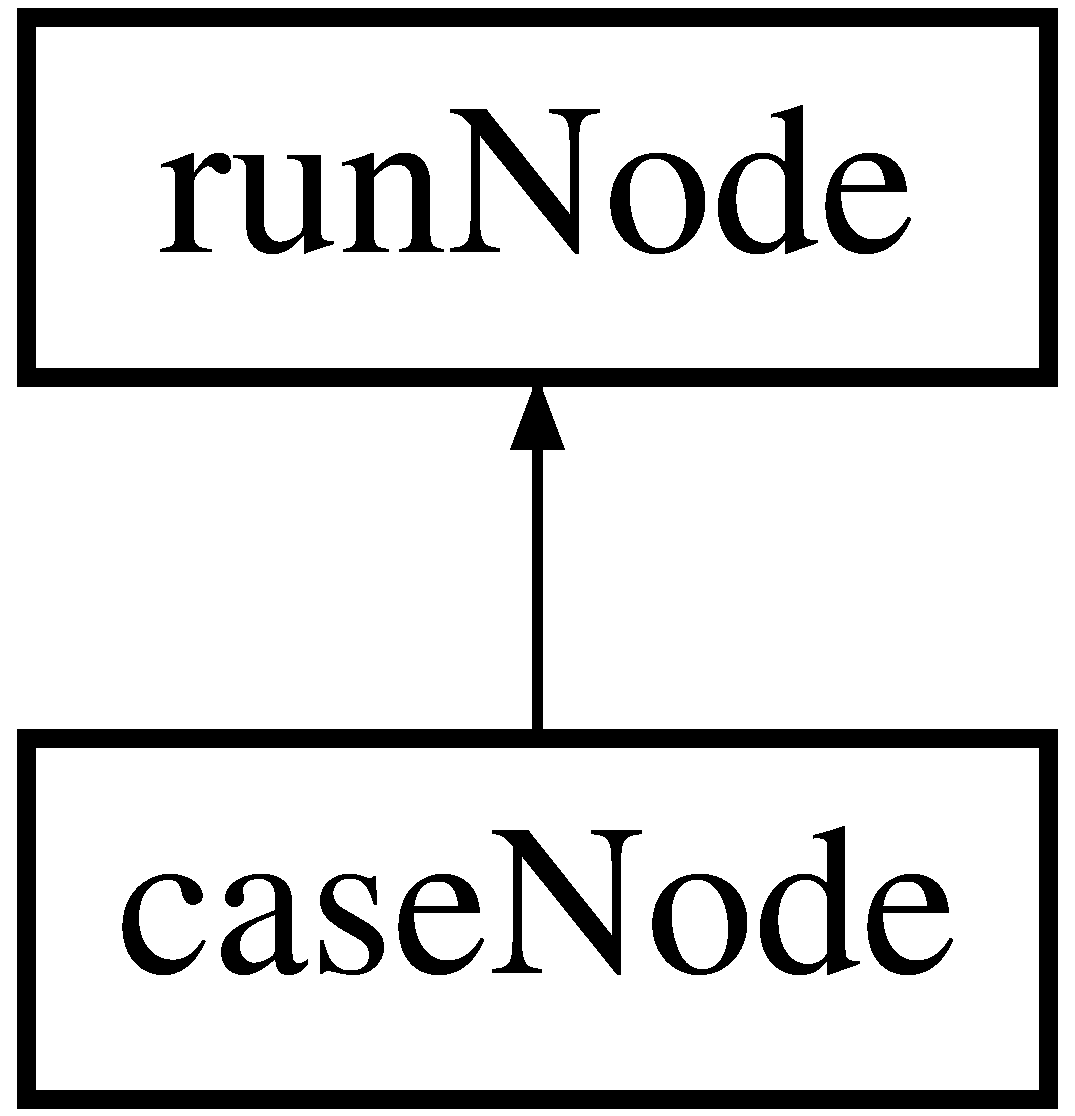
\includegraphics[height=2.000000cm]{classcaseNode}
\end{center}
\end{figure}
\subsection*{Métodos públicos}
\begin{DoxyCompactItemize}
\item 
\hyperlink{classcaseNode_a60431935cac670348d1af79dbc3fb58f}{case\-Node} (\hyperlink{classrunNode}{run\-Node} $\ast$exp, \hyperlink{classrunNode}{run\-Node} $\ast$cb, \hyperlink{classrunNode}{run\-Node} $\ast$cases)
\item 
void \hyperlink{classcaseNode_a10345cc86f9dec3ead3a71cc4d2fb2fa}{run} (\hyperlink{classrunNode}{run\-Node} $\ast$eval)
\item 
void \hyperlink{classcaseNode_a257a849756f7bcd0ccb0dc41a62783d9}{run} ()
\end{DoxyCompactItemize}
\subsection*{Otros miembros heredados}


\subsection{Descripción detallada}
Nodo casos switch. 

Este nodo representa una lista de casos switch. Un caso switch se define mediante una expresión para la comparación, un bloque de sentencias y un enlace al siguiente caso.

Para que el caso sea evaluado se ha de facilitar una expresión a evaluar. Se comprobará si la esta es igual a la expresión de comparación. Si lo es se ejecuta el bloque de sentencias de el caso y todos los casos siguientes. Si la evaluación dio un resultado negativo se comprueba el siguiente caso.

\begin{DoxySeeAlso}{Ver también}
\hyperlink{classswitchNode}{switch\-Node} 
\end{DoxySeeAlso}


\subsection{Documentación del constructor y destructor}
\hypertarget{classcaseNode_a60431935cac670348d1af79dbc3fb58f}{\index{case\-Node@{case\-Node}!case\-Node@{case\-Node}}
\index{case\-Node@{case\-Node}!caseNode@{case\-Node}}
\subsubsection[{case\-Node}]{\setlength{\rightskip}{0pt plus 5cm}case\-Node\-::case\-Node (
\begin{DoxyParamCaption}
\item[{{\bf run\-Node} $\ast$}]{exp, }
\item[{{\bf run\-Node} $\ast$}]{cb, }
\item[{{\bf run\-Node} $\ast$}]{cases}
\end{DoxyParamCaption}
)}}\label{classcaseNode_a60431935cac670348d1af79dbc3fb58f}
Constructor de la clase. 
\begin{DoxyParams}{Parámetros}
{\em exp} & Nodo que representa la expresión de comparación. \\
\hline
{\em cb} & Nodo que representa el bloque de sentencias del caso. \\
\hline
{\em cases} & Nodo que representa el siguiente caso. \\
\hline
\end{DoxyParams}


\subsection{Documentación de las funciones miembro}
\hypertarget{classcaseNode_a10345cc86f9dec3ead3a71cc4d2fb2fa}{\index{case\-Node@{case\-Node}!run@{run}}
\index{run@{run}!caseNode@{case\-Node}}
\subsubsection[{run}]{\setlength{\rightskip}{0pt plus 5cm}void case\-Node\-::run (
\begin{DoxyParamCaption}
\item[{{\bf run\-Node} $\ast$}]{eval}
\end{DoxyParamCaption}
)}}\label{classcaseNode_a10345cc86f9dec3ead3a71cc4d2fb2fa}
Método de ejecución del nodo. Evalúa un nodo dado como parámetro comparándolo con la expresión de comparación. Si el resultado es positivo se ejecuta el bloque de sentencias y los bloques de los casos siguientes. Si el resultado es falso se ejecuta la evaluación del caso siguiente. 
\begin{DoxyParams}{Parámetros}
{\em eval} & Nodo que representa la expresión que será comparada con la expresión del caso. \\
\hline
\end{DoxyParams}
\hypertarget{classcaseNode_a257a849756f7bcd0ccb0dc41a62783d9}{\index{case\-Node@{case\-Node}!run@{run}}
\index{run@{run}!caseNode@{case\-Node}}
\subsubsection[{run}]{\setlength{\rightskip}{0pt plus 5cm}void case\-Node\-::run (
\begin{DoxyParamCaption}
{}
\end{DoxyParamCaption}
)\hspace{0.3cm}{\ttfamily [virtual]}}}\label{classcaseNode_a257a849756f7bcd0ccb0dc41a62783d9}
Método de ejecución. Ejecuta el caso sin llevar a cabo la evaluación, lo que conlleva la ejecución del bloque de sentencias y el caso siguiente. 

Implementa \hyperlink{classrunNode_a83c10df8148829b08e04153c93d69eec}{run\-Node}.



La documentación para esta clase fue generada a partir de los siguientes ficheros\-:\begin{DoxyCompactItemize}
\item 
trunk/src/run/stmts/\hyperlink{condStmtNode_8h}{cond\-Stmt\-Node.\-h}\item 
trunk/src/run/stmts/cond\-Stmt\-Node.\-cpp\end{DoxyCompactItemize}

\hypertarget{classcatNode}{\section{Referencia de la Clase cat\-Node}
\label{classcatNode}\index{cat\-Node@{cat\-Node}}
}


Nodo función concatenación.  




{\ttfamily \#include $<$str\-Op\-Node.\-h$>$}

Diagrama de herencias de cat\-Node\begin{figure}[H]
\begin{center}
\leavevmode
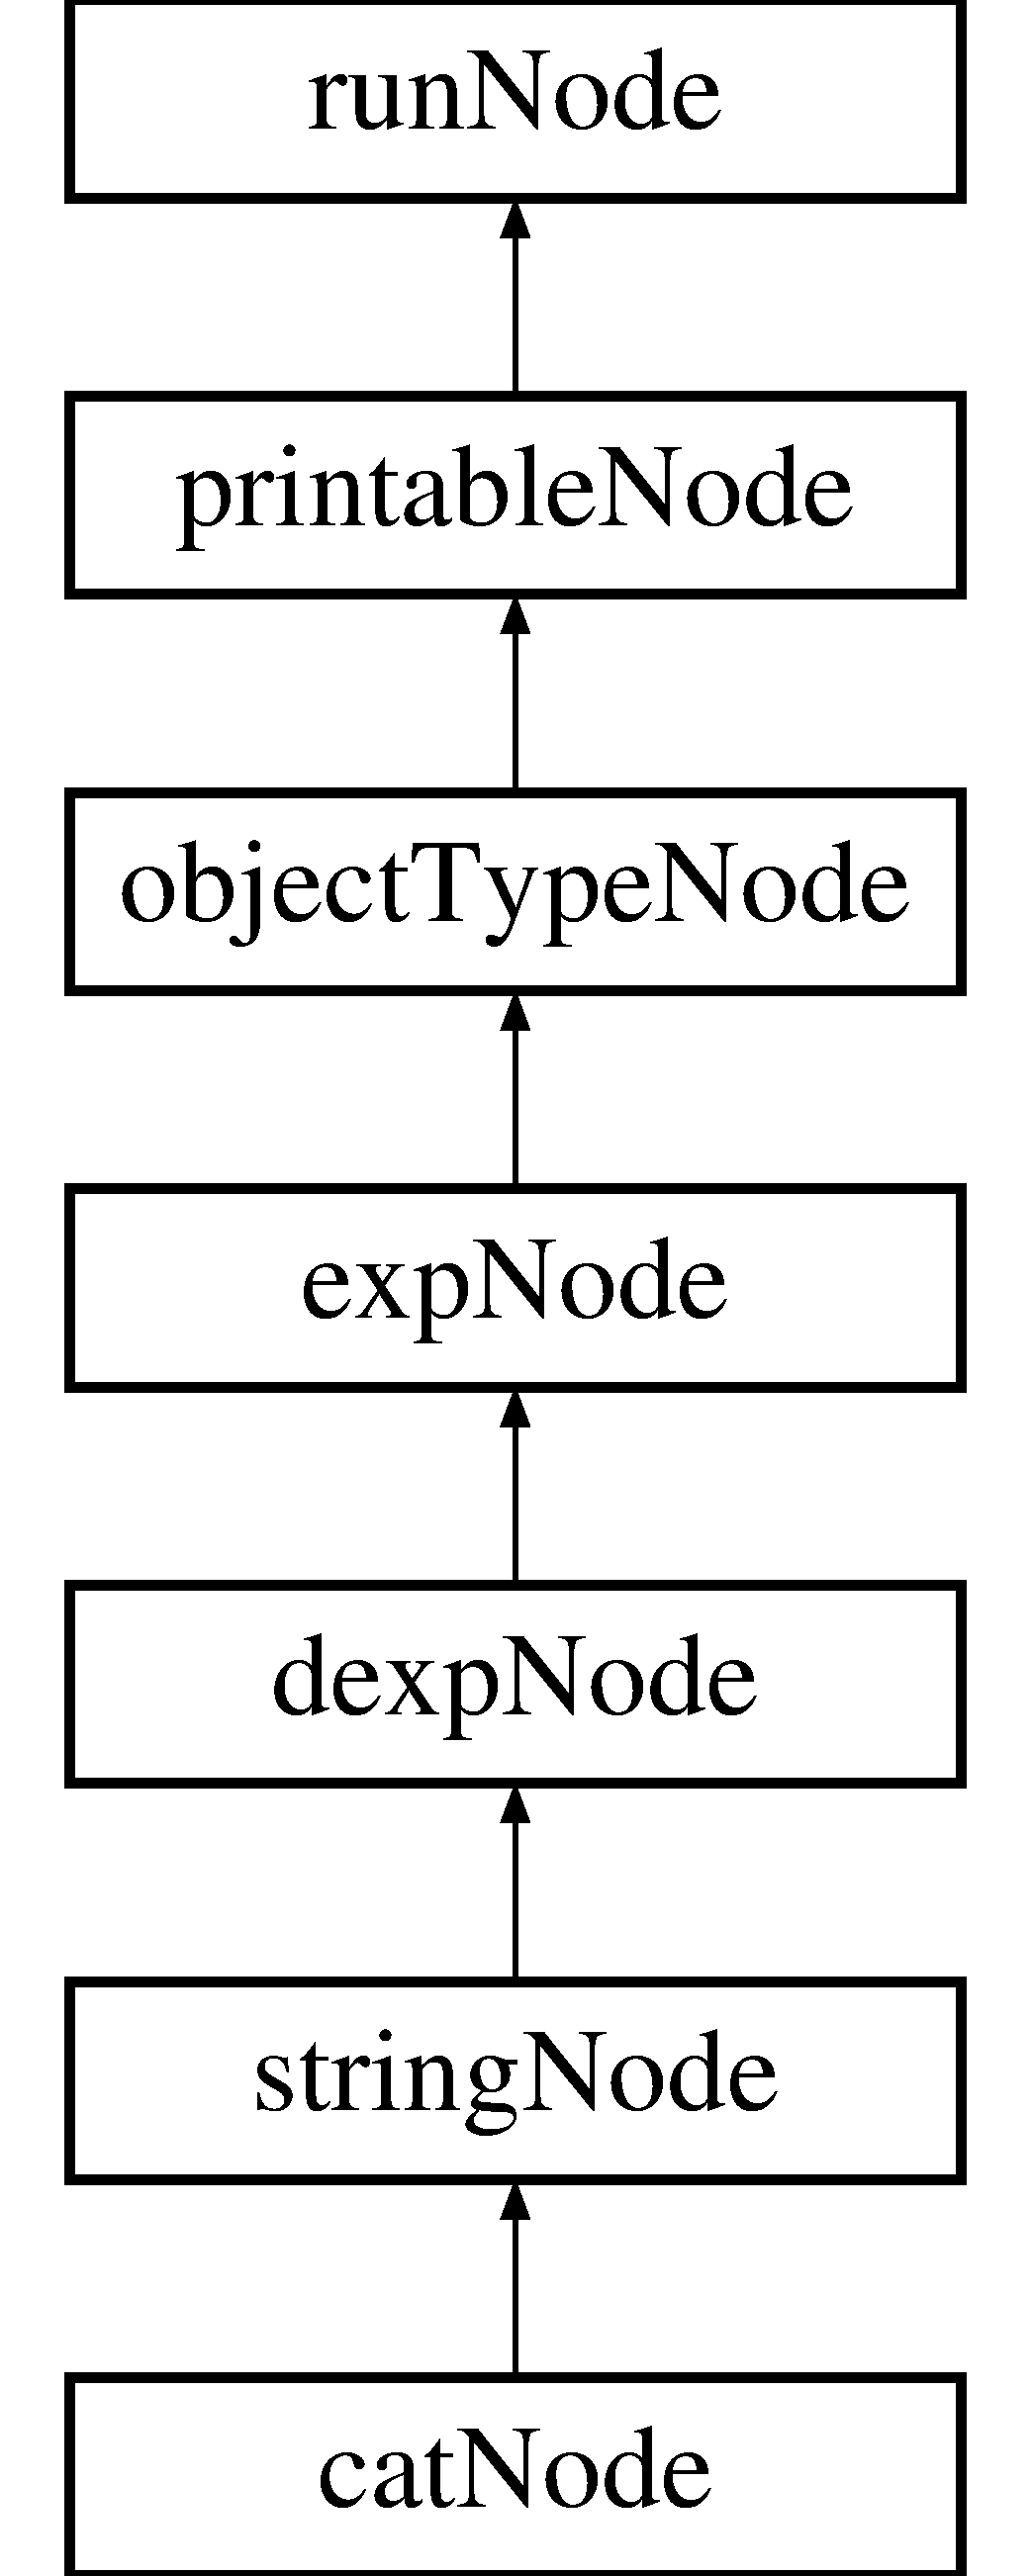
\includegraphics[height=7.000000cm]{classcatNode}
\end{center}
\end{figure}
\subsection*{Métodos públicos}
\begin{DoxyCompactItemize}
\item 
\hyperlink{classcatNode_a1ea19392b499f9383534fd26ccc9a6c8}{cat\-Node} (\hyperlink{classrunNode}{run\-Node} $\ast$node1, \hyperlink{classrunNode}{run\-Node} $\ast$node2, bool newline=false)
\item 
void \hyperlink{classcatNode_af6735016b3cb2477a94de79d7e1e1c62}{run} ()
\end{DoxyCompactItemize}
\subsection*{Métodos públicos estáticos}
\begin{DoxyCompactItemize}
\item 
static string \hyperlink{classcatNode_ae861e45f75270c8ba63e9bffd6bb7806}{do\-\_\-cat} (\hyperlink{classrunNode}{run\-Node} $\ast$op1, \hyperlink{classrunNode}{run\-Node} $\ast$op2, bool newline=false)
\end{DoxyCompactItemize}
\subsection*{Otros miembros heredados}


\subsection{Descripción detallada}
Nodo función concatenación. 

Este nodo implementa la operación concatenación sobre dos nodos asociados.

Si algún nodo no es una cadena de caracteres, fuerza la conversión a este tipo para realizar la operación

El resultado de evaluar la expresión es un valor cadena de caracteres. 

\subsection{Documentación del constructor y destructor}
\hypertarget{classcatNode_a1ea19392b499f9383534fd26ccc9a6c8}{\index{cat\-Node@{cat\-Node}!cat\-Node@{cat\-Node}}
\index{cat\-Node@{cat\-Node}!catNode@{cat\-Node}}
\subsubsection[{cat\-Node}]{\setlength{\rightskip}{0pt plus 5cm}cat\-Node\-::cat\-Node (
\begin{DoxyParamCaption}
\item[{{\bf run\-Node} $\ast$}]{node1, }
\item[{{\bf run\-Node} $\ast$}]{node2, }
\item[{bool}]{newline = {\ttfamily false}}
\end{DoxyParamCaption}
)}}\label{classcatNode_a1ea19392b499f9383534fd26ccc9a6c8}
Constructor de la clase. Asocia el nodo operador a dos nodos. 
\begin{DoxyParams}{Parámetros}
{\em node1} & Primer nodo operando. \\
\hline
{\em node2} & Sengundo nodo operando. \\
\hline
{\em newline} & Determina si se debe concatenar un salto de línea al resultado de la operación \\
\hline
\end{DoxyParams}


\subsection{Documentación de las funciones miembro}
\hypertarget{classcatNode_ae861e45f75270c8ba63e9bffd6bb7806}{\index{cat\-Node@{cat\-Node}!do\-\_\-cat@{do\-\_\-cat}}
\index{do\-\_\-cat@{do\-\_\-cat}!catNode@{cat\-Node}}
\subsubsection[{do\-\_\-cat}]{\setlength{\rightskip}{0pt plus 5cm}string cat\-Node\-::do\-\_\-cat (
\begin{DoxyParamCaption}
\item[{{\bf run\-Node} $\ast$}]{op1, }
\item[{{\bf run\-Node} $\ast$}]{op2, }
\item[{bool}]{newline = {\ttfamily false}}
\end{DoxyParamCaption}
)\hspace{0.3cm}{\ttfamily [static]}}}\label{classcatNode_ae861e45f75270c8ba63e9bffd6bb7806}
Ejecuta la operación concatenación sobre dos nodos dados. 
\begin{DoxyParams}{Parámetros}
{\em node1} & Primer nodo operando. \\
\hline
{\em node2} & Sengundo nodo operando. \\
\hline
{\em newline} & Determina si se debe concatenar un salto de línea al resultado de la operación \\
\hline
\end{DoxyParams}
\begin{DoxyReturn}{Devuelve}
Resultado de la operación. 
\end{DoxyReturn}
\hypertarget{classcatNode_af6735016b3cb2477a94de79d7e1e1c62}{\index{cat\-Node@{cat\-Node}!run@{run}}
\index{run@{run}!catNode@{cat\-Node}}
\subsubsection[{run}]{\setlength{\rightskip}{0pt plus 5cm}void cat\-Node\-::run (
\begin{DoxyParamCaption}
{}
\end{DoxyParamCaption}
)\hspace{0.3cm}{\ttfamily [virtual]}}}\label{classcatNode_af6735016b3cb2477a94de79d7e1e1c62}
Método que ejecuta el nodo. Procede a la ejecución de los nodos asociados. Luego obtiene el valor cadena de caracteres del nodo mediante la operación concatención entre el valor textual de los dos nodos.

Concatena un salto de línea si asi se especifico en la inicialización. 

Implementa \hyperlink{classrunNode_a83c10df8148829b08e04153c93d69eec}{run\-Node}.



La documentación para esta clase fue generada a partir de los siguientes ficheros\-:\begin{DoxyCompactItemize}
\item 
trunk/src/run/operators/\hyperlink{strOpNode_8h}{str\-Op\-Node.\-h}\item 
trunk/src/run/operators/str\-Op\-Node.\-cpp\end{DoxyCompactItemize}

\hypertarget{classclassNode}{\section{Referencia de la Clase class\-Node}
\label{classclassNode}\index{class\-Node@{class\-Node}}
}


Nodo clase.  




{\ttfamily \#include $<$class\-Node.\-h$>$}

Diagrama de herencias de class\-Node\begin{figure}[H]
\begin{center}
\leavevmode
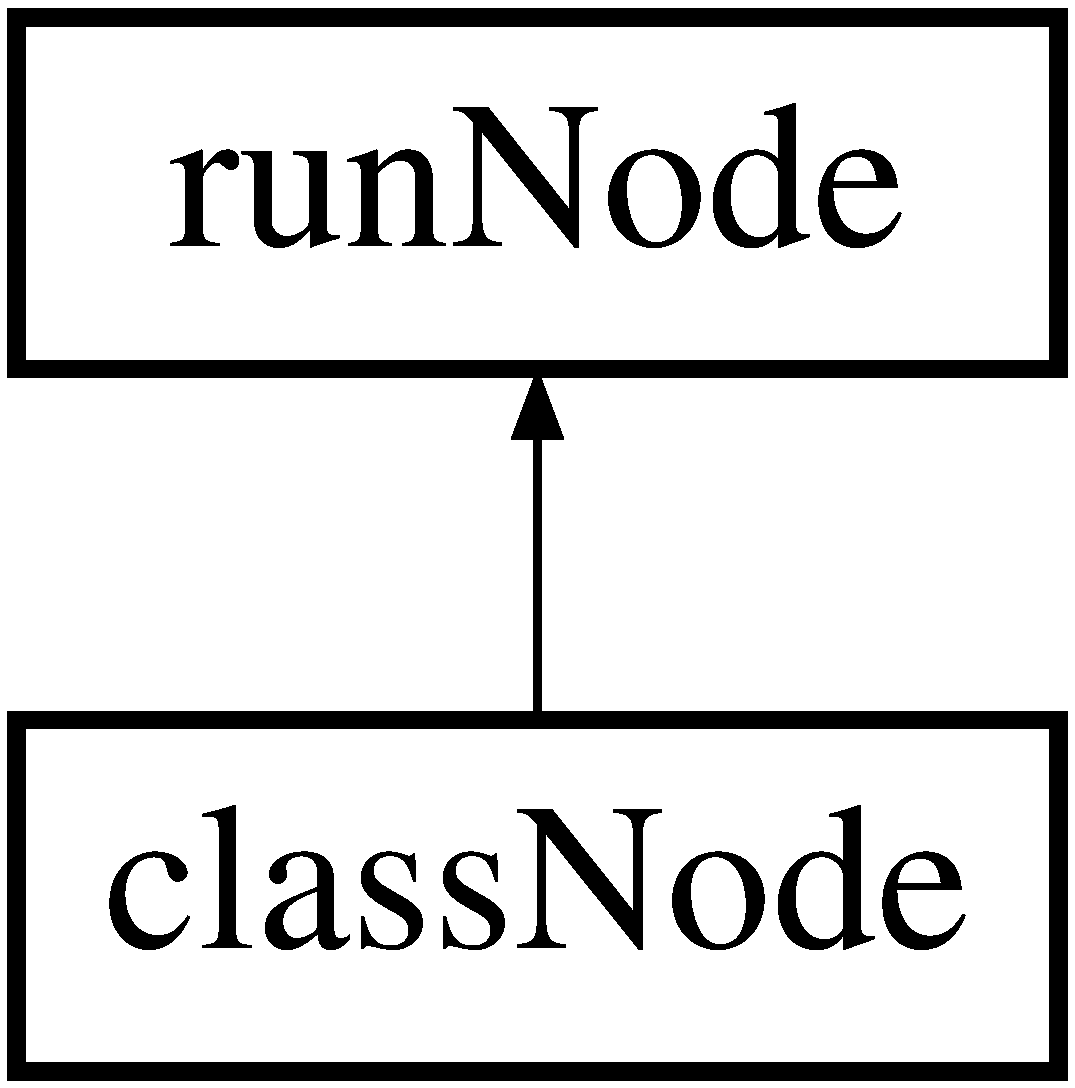
\includegraphics[height=2.000000cm]{classclassNode}
\end{center}
\end{figure}
\subsection*{Métodos públicos}
\begin{DoxyCompactItemize}
\item 
\hyperlink{classclassNode_aae32a053594c335e954a065152583727}{class\-Node} (\hyperlink{classclassNode}{class\-Node} $\ast$node)
\item 
\hyperlink{classclassNode_a7b5f4a91590e3aaf8b4271b157052d25}{class\-Node} (\hyperlink{classrunNode}{run\-Node} $\ast$id, \hyperlink{classrunNode}{run\-Node} $\ast$body, \hyperlink{classrunNode}{run\-Node} $\ast$extends=N\-U\-L\-L)
\item 
void \hyperlink{classclassNode_a65ea61be38e2ecbec6c7766951819939}{run} ()
\item 
\hyperlink{classrunNode}{run\-Node} $\ast$ \hyperlink{classclassNode_a5c58494486e9d1a856d8cdd271875867}{newcall} (\hyperlink{classrunNode}{run\-Node} $\ast$params)
\item 
\hyperlink{classsTable}{s\-Table} $\ast$ \hyperlink{classclassNode_abe7e603b04e733ebdbd0b8816b157cdc}{inside\-Table} () const 
\item 
\hyperlink{classclassNode}{class\-Node} $\ast$ \hyperlink{classclassNode_ab30594178fcfc96d0ce492323b9d3fbd}{get\-Extend\-Class} ()
\item 
\hyperlink{classrunNode}{run\-Node} $\ast$ \hyperlink{classclassNode_aad765264cfeff116c3155dc666fd6fb1}{get\-I\-D} ()
\item 
string \hyperlink{classclassNode_adee266b216dc087f11dd8adc6ea8ad5a}{name} ()
\item 
\hyperlink{classrunNode}{run\-Node} $\ast$ \hyperlink{classclassNode_a19f2361cff152d4d98176ea835f9baa1}{get\-Method} (\hyperlink{classrunNode}{run\-Node} $\ast$key)
\item 
\hyperlink{classrefNode}{ref\-Node} $\ast$ \hyperlink{classclassNode_a19369f3ce811e8f24ef8bc2e11bbe4d0}{get\-Method\-Ref} (\hyperlink{classrunNode}{run\-Node} $\ast$key)
\item 
void \hyperlink{classclassNode_ae3e5d11def9f49cc359bc40d2e77eabb}{set\-Method} (\hyperlink{classrunNode}{run\-Node} $\ast$key, \hyperlink{classrunNode}{run\-Node} $\ast$func)
\item 
\hyperlink{classrunNode}{run\-Node} $\ast$ \hyperlink{classclassNode_aa73ab0f885a76cfb42cb15baa983c0d6}{get\-From\-Static} (\hyperlink{classrunNode}{run\-Node} $\ast$key)
\item 
void \hyperlink{classclassNode_ae78654f623cfe5de2e421bd84f8d41f0}{set\-From\-Static} (\hyperlink{classrunNode}{run\-Node} $\ast$key, \hyperlink{classrunNode}{run\-Node} $\ast$val)
\item 
\hyperlink{classrunNode}{run\-Node} $\ast$ \hyperlink{classclassNode_a12cf5820b06a161bdb04c7a5fe430658}{to\-Object} ()
\end{DoxyCompactItemize}
\subsection*{Otros miembros heredados}


\subsection{Descripción detallada}
Nodo clase. 

Un nodo clase representa la definición de una clase. Una clase es una estructura funcional utilizada en la programación orientada a objetos.

Un nodo clase sirve como interfaz para definir y manipular las clases en ejecución.

Todo nodo clase tiene un contexto de tablas de símbolos donde se referencia a los atributos y métodos de la misma.

Para inicializar un nodo clase se precisa del identificador de la misma y un cuerpo.

El cuerpo de la clase consiste en una serie de sentencias, que por limitaciones de gramática sólo pueden ser declaraciones de funciones o variables.

La ejecución de un nodo clase se corresponde con la declaración de la misma. Primero crea una referencia a si misma en la tabla de clases activa. Luego crea un nuevo contexto de tablas de símbolos, que usará de forma interna. Para finalizar cambia el contexto activo al interno y se lleva a cabo la ejecución del cuerpo.

Los nodos funciones declarados en el cuerpo de la clase serán referenciados desde la tabla de funciones de la clase y son considerados los métodos de la misma. De igual forma las variables son referenciadas mediante la tabla de variables y son consideradas como los atributos.

Una determinada clase puede extender a otra, lo que significa que heredará sus métodos y atributos.

Los nodos clase presentan un mecanismo para crear nuevas instancias de los mismos denominadas objetos. Este mecanismo es utilizado por nodos como el nodo \char`\"{}nueva instancia\char`\"{} (\begin{DoxySeeAlso}{Ver también}
\hyperlink{classnewNode}{new\-Node}). Cuando se crear una nueva instancia se genera una copia de la tabla de símbolos de variables en un nodo de tipo objeto Este objeto además referencia a la clase para acceder a los métodos. El objeto se puede asignar a un nodo id como si fuera un tipo de dato, guardándose asi una referencia en la tabla de variables activa.
\end{DoxySeeAlso}
Las clases disponen de un contexto interno con tablas para funciones y variables que será aplicables a los objetos como atributos y métodos. Además disponen de un contexto estático que guarda los métodos y atributos aplicables a la propia clase. 

\subsection{Documentación del constructor y destructor}
\hypertarget{classclassNode_aae32a053594c335e954a065152583727}{\index{class\-Node@{class\-Node}!class\-Node@{class\-Node}}
\index{class\-Node@{class\-Node}!classNode@{class\-Node}}
\subsubsection[{class\-Node}]{\setlength{\rightskip}{0pt plus 5cm}class\-Node\-::class\-Node (
\begin{DoxyParamCaption}
\item[{{\bf class\-Node} $\ast$}]{node}
\end{DoxyParamCaption}
)}}\label{classclassNode_aae32a053594c335e954a065152583727}
Constructor copia. Crea un nodo clase a partir de otro. Para ello referencia al cuerpo y al identificador del nodo clase dado, y copia la tabla de símbolos interna. \hypertarget{classclassNode_a7b5f4a91590e3aaf8b4271b157052d25}{\index{class\-Node@{class\-Node}!class\-Node@{class\-Node}}
\index{class\-Node@{class\-Node}!classNode@{class\-Node}}
\subsubsection[{class\-Node}]{\setlength{\rightskip}{0pt plus 5cm}class\-Node\-::class\-Node (
\begin{DoxyParamCaption}
\item[{{\bf run\-Node} $\ast$}]{id, }
\item[{{\bf run\-Node} $\ast$}]{body, }
\item[{{\bf run\-Node} $\ast$}]{extends = {\ttfamily NULL}}
\end{DoxyParamCaption}
)}}\label{classclassNode_a7b5f4a91590e3aaf8b4271b157052d25}
Constructor que inicializa un nodo clase a partir de un nodo identificador y un nodo cuerpo. 
\begin{DoxyParams}{Parámetros}
{\em id} & Identificador de la clase. \\
\hline
{\em body} & Cuerpo de la clase. \\
\hline
{\em extends} & Clase de la que extiende si es el caso. \\
\hline
\end{DoxyParams}


\subsection{Documentación de las funciones miembro}
\hypertarget{classclassNode_ab30594178fcfc96d0ce492323b9d3fbd}{\index{class\-Node@{class\-Node}!get\-Extend\-Class@{get\-Extend\-Class}}
\index{get\-Extend\-Class@{get\-Extend\-Class}!classNode@{class\-Node}}
\subsubsection[{get\-Extend\-Class}]{\setlength{\rightskip}{0pt plus 5cm}{\bf class\-Node}$\ast$ class\-Node\-::get\-Extend\-Class (
\begin{DoxyParamCaption}
{}
\end{DoxyParamCaption}
)\hspace{0.3cm}{\ttfamily [inline]}}}\label{classclassNode_ab30594178fcfc96d0ce492323b9d3fbd}
Obtiene la clase padre con la que fue inicializada. \begin{DoxyReturn}{Devuelve}
Clase padre. 
\end{DoxyReturn}
\hypertarget{classclassNode_aa73ab0f885a76cfb42cb15baa983c0d6}{\index{class\-Node@{class\-Node}!get\-From\-Static@{get\-From\-Static}}
\index{get\-From\-Static@{get\-From\-Static}!classNode@{class\-Node}}
\subsubsection[{get\-From\-Static}]{\setlength{\rightskip}{0pt plus 5cm}{\bf run\-Node} $\ast$ class\-Node\-::get\-From\-Static (
\begin{DoxyParamCaption}
\item[{{\bf run\-Node} $\ast$}]{key}
\end{DoxyParamCaption}
)}}\label{classclassNode_aa73ab0f885a76cfb42cb15baa983c0d6}
Obtiene un método estático de la clase a partir de una clave. 
\begin{DoxyParams}{Parámetros}
{\em key} & Nombre del método. \\
\hline
\end{DoxyParams}
\begin{DoxyReturn}{Devuelve}
Método estático correspondiente a la clave. 
\end{DoxyReturn}
\hypertarget{classclassNode_aad765264cfeff116c3155dc666fd6fb1}{\index{class\-Node@{class\-Node}!get\-I\-D@{get\-I\-D}}
\index{get\-I\-D@{get\-I\-D}!classNode@{class\-Node}}
\subsubsection[{get\-I\-D}]{\setlength{\rightskip}{0pt plus 5cm}{\bf run\-Node}$\ast$ class\-Node\-::get\-I\-D (
\begin{DoxyParamCaption}
{}
\end{DoxyParamCaption}
)\hspace{0.3cm}{\ttfamily [inline]}}}\label{classclassNode_aad765264cfeff116c3155dc666fd6fb1}
Obtiene el identificador con el que fue inicializada. \begin{DoxyReturn}{Devuelve}
I\-D de la clase. 
\end{DoxyReturn}
\hypertarget{classclassNode_a19f2361cff152d4d98176ea835f9baa1}{\index{class\-Node@{class\-Node}!get\-Method@{get\-Method}}
\index{get\-Method@{get\-Method}!classNode@{class\-Node}}
\subsubsection[{get\-Method}]{\setlength{\rightskip}{0pt plus 5cm}{\bf run\-Node} $\ast$ class\-Node\-::get\-Method (
\begin{DoxyParamCaption}
\item[{{\bf run\-Node} $\ast$}]{key}
\end{DoxyParamCaption}
)}}\label{classclassNode_a19f2361cff152d4d98176ea835f9baa1}
A partir de una clave obtiene el método cuyo identificador se corresponde con la misma. Si no existe se devuelve N\-U\-L\-L. 
\begin{DoxyParams}{Parámetros}
{\em key} & Nombre del método. \\
\hline
\end{DoxyParams}
\begin{DoxyReturn}{Devuelve}
Método correspondiente a la clave. 
\end{DoxyReturn}
\hypertarget{classclassNode_a19369f3ce811e8f24ef8bc2e11bbe4d0}{\index{class\-Node@{class\-Node}!get\-Method\-Ref@{get\-Method\-Ref}}
\index{get\-Method\-Ref@{get\-Method\-Ref}!classNode@{class\-Node}}
\subsubsection[{get\-Method\-Ref}]{\setlength{\rightskip}{0pt plus 5cm}{\bf ref\-Node} $\ast$ class\-Node\-::get\-Method\-Ref (
\begin{DoxyParamCaption}
\item[{{\bf run\-Node} $\ast$}]{key}
\end{DoxyParamCaption}
)}}\label{classclassNode_a19369f3ce811e8f24ef8bc2e11bbe4d0}
A partir de una clave obtiene la referencia al método cuyo identificador se corresponde con la misma. Si no existe se devuelve N\-U\-L\-L. 
\begin{DoxyParams}{Parámetros}
{\em key} & Nombre del método. \\
\hline
\end{DoxyParams}
\begin{DoxyReturn}{Devuelve}
Referencia al método correspondietne a la clave. 
\end{DoxyReturn}
\hypertarget{classclassNode_abe7e603b04e733ebdbd0b8816b157cdc}{\index{class\-Node@{class\-Node}!inside\-Table@{inside\-Table}}
\index{inside\-Table@{inside\-Table}!classNode@{class\-Node}}
\subsubsection[{inside\-Table}]{\setlength{\rightskip}{0pt plus 5cm}{\bf s\-Table}$\ast$ class\-Node\-::inside\-Table (
\begin{DoxyParamCaption}
{}
\end{DoxyParamCaption}
) const\hspace{0.3cm}{\ttfamily [inline]}}}\label{classclassNode_abe7e603b04e733ebdbd0b8816b157cdc}
Devuelve el contexto interno del nodo clase. \begin{DoxyReturn}{Devuelve}
Contexto interno. 
\end{DoxyReturn}
\hypertarget{classclassNode_adee266b216dc087f11dd8adc6ea8ad5a}{\index{class\-Node@{class\-Node}!name@{name}}
\index{name@{name}!classNode@{class\-Node}}
\subsubsection[{name}]{\setlength{\rightskip}{0pt plus 5cm}string class\-Node\-::name (
\begin{DoxyParamCaption}
{}
\end{DoxyParamCaption}
)\hspace{0.3cm}{\ttfamily [inline]}}}\label{classclassNode_adee266b216dc087f11dd8adc6ea8ad5a}
Obtiene el identificador de la clase como una cadena de caracteres. \begin{DoxyReturn}{Devuelve}
I\-D de la clase como cadena de caracteres. 
\end{DoxyReturn}
\hypertarget{classclassNode_a5c58494486e9d1a856d8cdd271875867}{\index{class\-Node@{class\-Node}!newcall@{newcall}}
\index{newcall@{newcall}!classNode@{class\-Node}}
\subsubsection[{newcall}]{\setlength{\rightskip}{0pt plus 5cm}{\bf run\-Node} $\ast$ class\-Node\-::newcall (
\begin{DoxyParamCaption}
\item[{{\bf run\-Node} $\ast$}]{params}
\end{DoxyParamCaption}
)}}\label{classclassNode_a5c58494486e9d1a856d8cdd271875867}
Crea y devuelve una instancia de la clase. Para ello copia la tabla de variables del contexto de la clase en un nodo objeto, y busca una función en la tabla de funciones correspondiente al nombre de la clase. Esta función, considerada constructor, será ejecutada con los parámetros indicados. \hypertarget{classclassNode_a65ea61be38e2ecbec6c7766951819939}{\index{class\-Node@{class\-Node}!run@{run}}
\index{run@{run}!classNode@{class\-Node}}
\subsubsection[{run}]{\setlength{\rightskip}{0pt plus 5cm}void class\-Node\-::run (
\begin{DoxyParamCaption}
{}
\end{DoxyParamCaption}
)\hspace{0.3cm}{\ttfamily [virtual]}}}\label{classclassNode_a65ea61be38e2ecbec6c7766951819939}
Lleva a cabo la ejecución del nodo clase correspondiente a la declaración de la misma. Para ello crea una referencia en la tabla de clases activa a si misma, genera el contexto interno, y luego, tras cambiar el contexto en uso, ejecuta el cuerpo. 

Implementa \hyperlink{classrunNode_a83c10df8148829b08e04153c93d69eec}{run\-Node}.

\hypertarget{classclassNode_ae78654f623cfe5de2e421bd84f8d41f0}{\index{class\-Node@{class\-Node}!set\-From\-Static@{set\-From\-Static}}
\index{set\-From\-Static@{set\-From\-Static}!classNode@{class\-Node}}
\subsubsection[{set\-From\-Static}]{\setlength{\rightskip}{0pt plus 5cm}void class\-Node\-::set\-From\-Static (
\begin{DoxyParamCaption}
\item[{{\bf run\-Node} $\ast$}]{key, }
\item[{{\bf run\-Node} $\ast$}]{val}
\end{DoxyParamCaption}
)}}\label{classclassNode_ae78654f623cfe5de2e421bd84f8d41f0}
Asocia una función como método estático de la clase con el identificador dado. 
\begin{DoxyParams}{Parámetros}
{\em key} & Clave que se utilizará como identificador. \\
\hline
{\em func} & Función que se asociará como método estático. \\
\hline
\end{DoxyParams}
\hypertarget{classclassNode_ae3e5d11def9f49cc359bc40d2e77eabb}{\index{class\-Node@{class\-Node}!set\-Method@{set\-Method}}
\index{set\-Method@{set\-Method}!classNode@{class\-Node}}
\subsubsection[{set\-Method}]{\setlength{\rightskip}{0pt plus 5cm}void class\-Node\-::set\-Method (
\begin{DoxyParamCaption}
\item[{{\bf run\-Node} $\ast$}]{key, }
\item[{{\bf run\-Node} $\ast$}]{func}
\end{DoxyParamCaption}
)}}\label{classclassNode_ae3e5d11def9f49cc359bc40d2e77eabb}
Asocia una función como método de la clase con el identificador dado. 
\begin{DoxyParams}{Parámetros}
{\em key} & Clave que se utilizará como identificador. \\
\hline
{\em func} & Función que se asociará como método. \\
\hline
\end{DoxyParams}
\hypertarget{classclassNode_a12cf5820b06a161bdb04c7a5fe430658}{\index{class\-Node@{class\-Node}!to\-Object@{to\-Object}}
\index{to\-Object@{to\-Object}!classNode@{class\-Node}}
\subsubsection[{to\-Object}]{\setlength{\rightskip}{0pt plus 5cm}{\bf run\-Node} $\ast$ class\-Node\-::to\-Object (
\begin{DoxyParamCaption}
{}
\end{DoxyParamCaption}
)}}\label{classclassNode_a12cf5820b06a161bdb04c7a5fe430658}
Devuelve un objeto con una tabla de símbolos correspondiente a la tabla de variables de la clase. Además asocia la clase al objeto. \begin{DoxyReturn}{Devuelve}
Objeto instancia de la clase. 
\end{DoxyReturn}


La documentación para esta clase fue generada a partir de los siguientes ficheros\-:\begin{DoxyCompactItemize}
\item 
trunk/src/run/table/\hyperlink{classNode_8h}{class\-Node.\-h}\item 
trunk/src/run/table/class\-Node.\-cpp\end{DoxyCompactItemize}

\hypertarget{structcmp__runNode}{\section{Referencia de la Estructura cmp\-\_\-run\-Node}
\label{structcmp__runNode}\index{cmp\-\_\-run\-Node@{cmp\-\_\-run\-Node}}
}


{\ttfamily \#include $<$run\-Tree.\-h$>$}

\subsection*{Métodos públicos}
\begin{DoxyCompactItemize}
\item 
bool \hyperlink{structcmp__runNode_a715c67ee7063bfafcf994b2427bfa584}{operator()} (\hyperlink{classrunNode}{run\-Node} $\ast$node1, \hyperlink{classrunNode}{run\-Node} $\ast$node2)
\end{DoxyCompactItemize}


\subsection{Descripción detallada}
Estructura que define la comparación de elementos \hyperlink{classrunNode}{run\-Node}.

Esta estructura hace posible la ordenación de elementos puntero a nodo ejecutable por su valor interno. 

\subsection{Documentación de las funciones miembro}
\hypertarget{structcmp__runNode_a715c67ee7063bfafcf994b2427bfa584}{\index{cmp\-\_\-run\-Node@{cmp\-\_\-run\-Node}!operator()@{operator()}}
\index{operator()@{operator()}!cmp_runNode@{cmp\-\_\-run\-Node}}
\subsubsection[{operator()}]{\setlength{\rightskip}{0pt plus 5cm}bool cmp\-\_\-run\-Node\-::operator() (
\begin{DoxyParamCaption}
\item[{{\bf run\-Node} $\ast$}]{node1, }
\item[{{\bf run\-Node} $\ast$}]{node2}
\end{DoxyParamCaption}
)}}\label{structcmp__runNode_a715c67ee7063bfafcf994b2427bfa584}
Realiza la comparación del valor de $\ast$node1 con el valor de $\ast$node2 Y determina si $\ast$node1 $<$ $\ast$node2 

La documentación para esta estructura fue generada a partir de los siguientes ficheros\-:\begin{DoxyCompactItemize}
\item 
trunk/src/run/tree/\hyperlink{runTree_8h}{run\-Tree.\-h}\item 
trunk/src/run/tree/exp\-Node.\-cpp\end{DoxyCompactItemize}

\hypertarget{classcontextFunction}{\section{Referencia de la Clase context\-Function}
\label{classcontextFunction}\index{context\-Function@{context\-Function}}
}


Función de contexto.  




{\ttfamily \#include $<$func\-Node.\-h$>$}

Diagrama de herencias de context\-Function\begin{figure}[H]
\begin{center}
\leavevmode
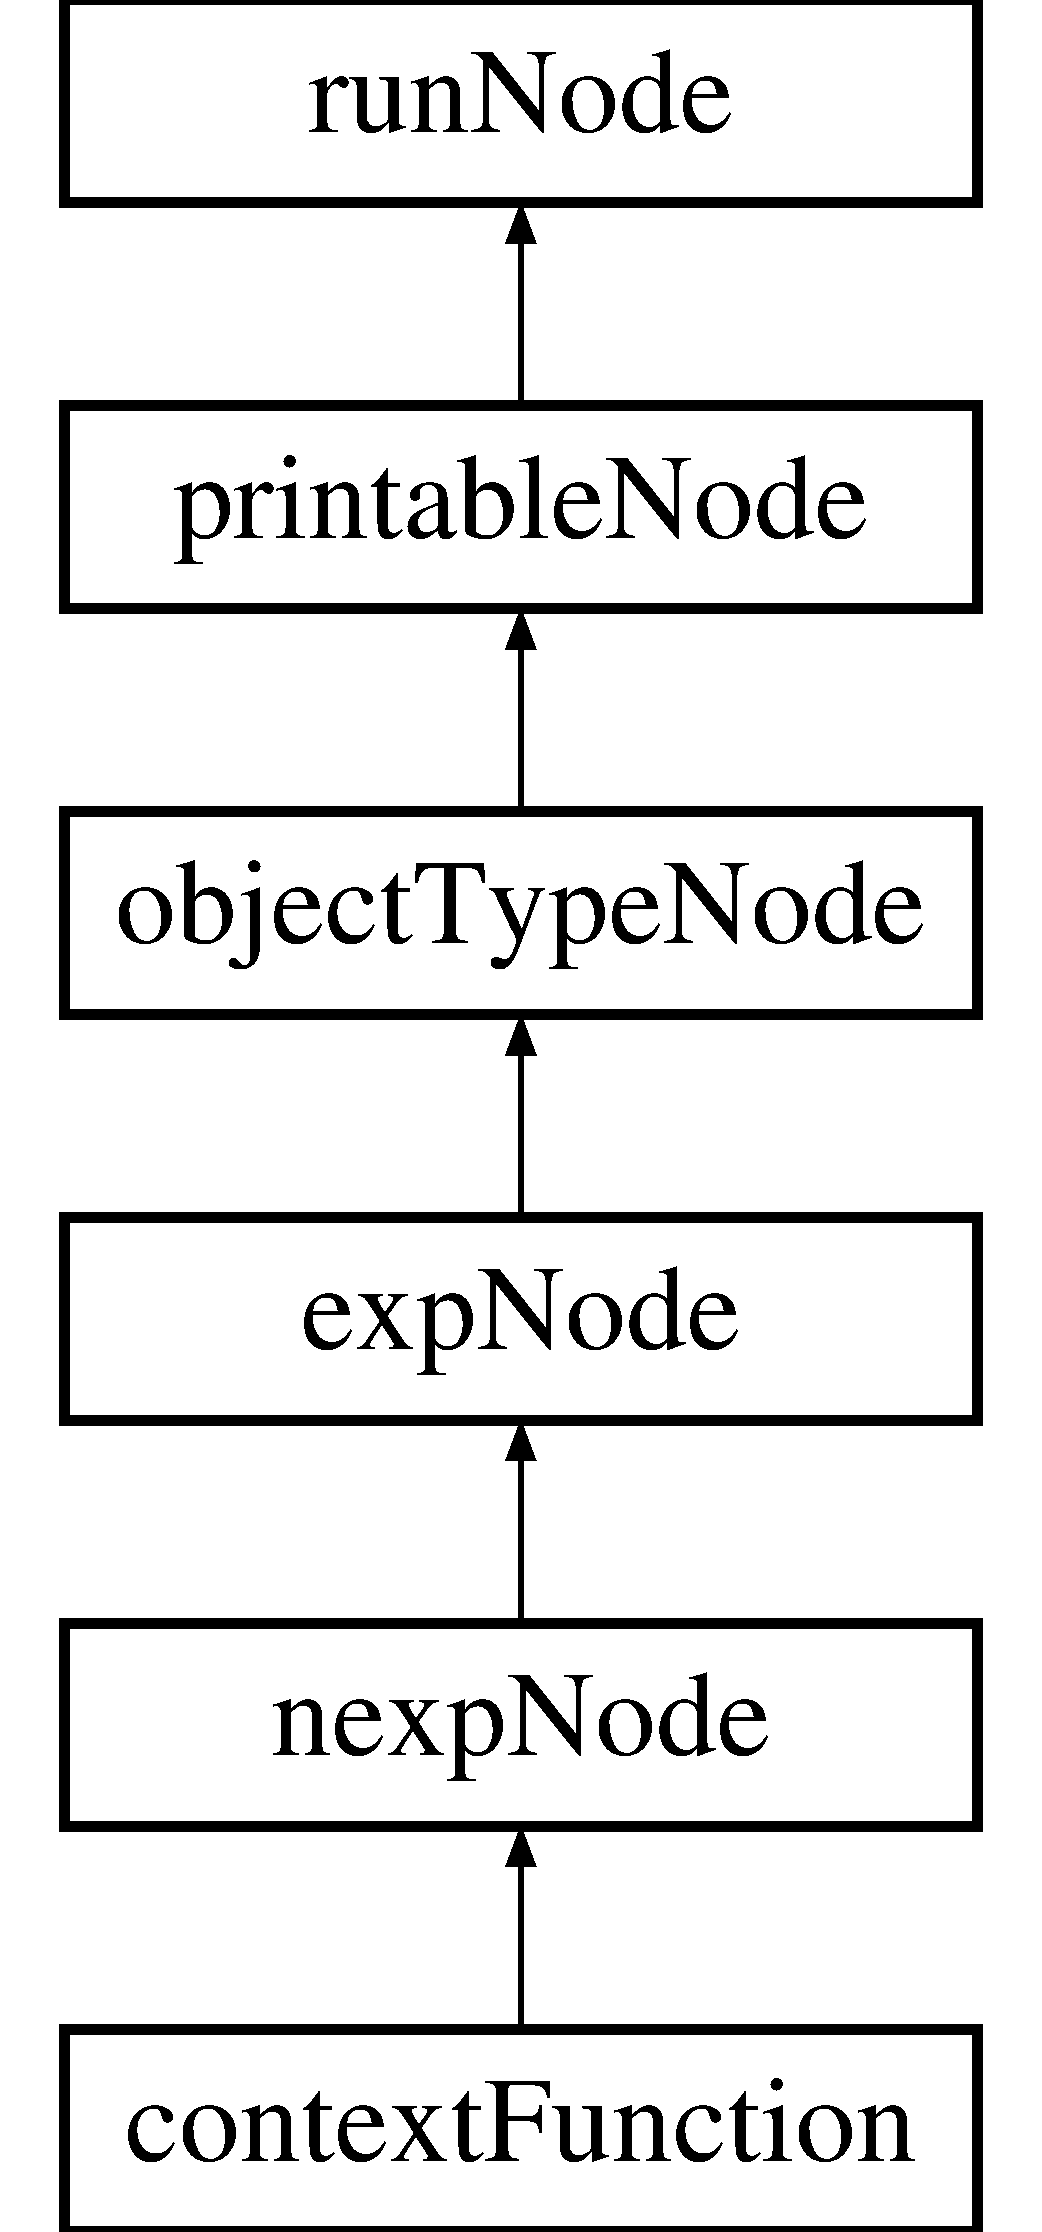
\includegraphics[height=6.000000cm]{classcontextFunction}
\end{center}
\end{figure}
\subsection*{Métodos públicos}
\begin{DoxyCompactItemize}
\item 
\hyperlink{classcontextFunction_ad159e580cf37d4d79cedc0bf33bb33f6}{context\-Function} ()
\item 
void \hyperlink{classcontextFunction_ad726824c42f4968600df92d75609d6ae}{run} ()
\end{DoxyCompactItemize}
\subsection*{Otros miembros heredados}


\subsection{Descripción detallada}
Función de contexto. 

Nodo que obtiene la función de contexto. Esta es la función actualmente en ejecución o la función utilizada en un decorador. 

\subsection{Documentación del constructor y destructor}
\hypertarget{classcontextFunction_ad159e580cf37d4d79cedc0bf33bb33f6}{\index{context\-Function@{context\-Function}!context\-Function@{context\-Function}}
\index{context\-Function@{context\-Function}!contextFunction@{context\-Function}}
\subsubsection[{context\-Function}]{\setlength{\rightskip}{0pt plus 5cm}context\-Function\-::context\-Function (
\begin{DoxyParamCaption}
{}
\end{DoxyParamCaption}
)}}\label{classcontextFunction_ad159e580cf37d4d79cedc0bf33bb33f6}
Constructor de la clase. 

\subsection{Documentación de las funciones miembro}
\hypertarget{classcontextFunction_ad726824c42f4968600df92d75609d6ae}{\index{context\-Function@{context\-Function}!run@{run}}
\index{run@{run}!contextFunction@{context\-Function}}
\subsubsection[{run}]{\setlength{\rightskip}{0pt plus 5cm}void context\-Function\-::run (
\begin{DoxyParamCaption}
{}
\end{DoxyParamCaption}
)\hspace{0.3cm}{\ttfamily [virtual]}}}\label{classcontextFunction_ad726824c42f4968600df92d75609d6ae}
Toma como referencia la función de contexto. Esta es la función actual. 

Implementa \hyperlink{classrunNode_a83c10df8148829b08e04153c93d69eec}{run\-Node}.



La documentación para esta clase fue generada a partir de los siguientes ficheros\-:\begin{DoxyCompactItemize}
\item 
trunk/src/run/table/\hyperlink{funcNode_8h}{func\-Node.\-h}\item 
trunk/src/run/table/func\-Node.\-cpp\end{DoxyCompactItemize}

\hypertarget{classcontinueException}{\section{Referencia de la Clase continue\-Exception}
\label{classcontinueException}\index{continue\-Exception@{continue\-Exception}}
}


Excepción lanzada cuando se produce una sentencia continue.  




{\ttfamily \#include $<$loop\-Stmt\-Node.\-h$>$}



Herencias exception.

\subsection*{Métodos públicos}
\begin{DoxyCompactItemize}
\item 
\hyperlink{classcontinueException_a025267d9810bc2d480353adb6ee43d86}{continue\-Exception} (int n=1)
\item 
const char $\ast$ \hyperlink{classcontinueException_acf175be01b6e026c7e1354e587459f75}{what} () const   throw ()
\item 
void \hyperlink{classcontinueException_aa379e96a9c81362522a9d8535ce7ad05}{end} ()
\item 
bool \hyperlink{classcontinueException_a3ba0b14f7e927fe2dced4624bbfe90fc}{islast} ()
\end{DoxyCompactItemize}


\subsection{Descripción detallada}
Excepción lanzada cuando se produce una sentencia continue. 

Esta excepción es lanzada cuando se ejecuta una sentencia continue, será atrapada por una sentencia iterativa y producirá que esta avance hasta la siguiente iteración.

Es posible indicar mediante un entero el número de sentencias iterativas anidadas que serán saltadas 

\subsection{Documentación del constructor y destructor}
\hypertarget{classcontinueException_a025267d9810bc2d480353adb6ee43d86}{\index{continue\-Exception@{continue\-Exception}!continue\-Exception@{continue\-Exception}}
\index{continue\-Exception@{continue\-Exception}!continueException@{continue\-Exception}}
\subsubsection[{continue\-Exception}]{\setlength{\rightskip}{0pt plus 5cm}continue\-Exception\-::continue\-Exception (
\begin{DoxyParamCaption}
\item[{int}]{n = {\ttfamily 1}}
\end{DoxyParamCaption}
)}}\label{classcontinueException_a025267d9810bc2d480353adb6ee43d86}
Constructor de la clase. 
\begin{DoxyParams}{Parámetros}
{\em n} & Número de sentencias iterativas anidadas que serán saltadas. \\
\hline
\end{DoxyParams}


\subsection{Documentación de las funciones miembro}
\hypertarget{classcontinueException_aa379e96a9c81362522a9d8535ce7ad05}{\index{continue\-Exception@{continue\-Exception}!end@{end}}
\index{end@{end}!continueException@{continue\-Exception}}
\subsubsection[{end}]{\setlength{\rightskip}{0pt plus 5cm}void continue\-Exception\-::end (
\begin{DoxyParamCaption}
{}
\end{DoxyParamCaption}
)}}\label{classcontinueException_aa379e96a9c81362522a9d8535ce7ad05}
Si el número de bloques anidados es mayor que uno lanza una excepción continue decrementando el número de bloques anidados. \hypertarget{classcontinueException_a3ba0b14f7e927fe2dced4624bbfe90fc}{\index{continue\-Exception@{continue\-Exception}!islast@{islast}}
\index{islast@{islast}!continueException@{continue\-Exception}}
\subsubsection[{islast}]{\setlength{\rightskip}{0pt plus 5cm}bool continue\-Exception\-::islast (
\begin{DoxyParamCaption}
{}
\end{DoxyParamCaption}
)}}\label{classcontinueException_a3ba0b14f7e927fe2dced4624bbfe90fc}
Comprueba si es el último de los bloques anidados \begin{DoxyReturn}{Devuelve}
Booleano que indica si el bloque es el últimos de los bloques anidados que se desean saltar. 
\end{DoxyReturn}
\hypertarget{classcontinueException_acf175be01b6e026c7e1354e587459f75}{\index{continue\-Exception@{continue\-Exception}!what@{what}}
\index{what@{what}!continueException@{continue\-Exception}}
\subsubsection[{what}]{\setlength{\rightskip}{0pt plus 5cm}const char $\ast$ continue\-Exception\-::what (
\begin{DoxyParamCaption}
{}
\end{DoxyParamCaption}
) const throw  ) }}\label{classcontinueException_acf175be01b6e026c7e1354e587459f75}
Método que será llamado si la excepción no es capturada. Produciéndose un error 

La documentación para esta clase fue generada a partir de los siguientes ficheros\-:\begin{DoxyCompactItemize}
\item 
trunk/src/run/stmts/\hyperlink{loopStmtNode_8h}{loop\-Stmt\-Node.\-h}\item 
trunk/src/run/stmts/loop\-Stmt\-Node.\-cpp\end{DoxyCompactItemize}

\hypertarget{classcontinueNode}{\section{Referencia de la Clase continue\-Node}
\label{classcontinueNode}\index{continue\-Node@{continue\-Node}}
}


Nodo sentencia continue.  




{\ttfamily \#include $<$loop\-Stmt\-Node.\-h$>$}

Diagrama de herencias de continue\-Node\begin{figure}[H]
\begin{center}
\leavevmode
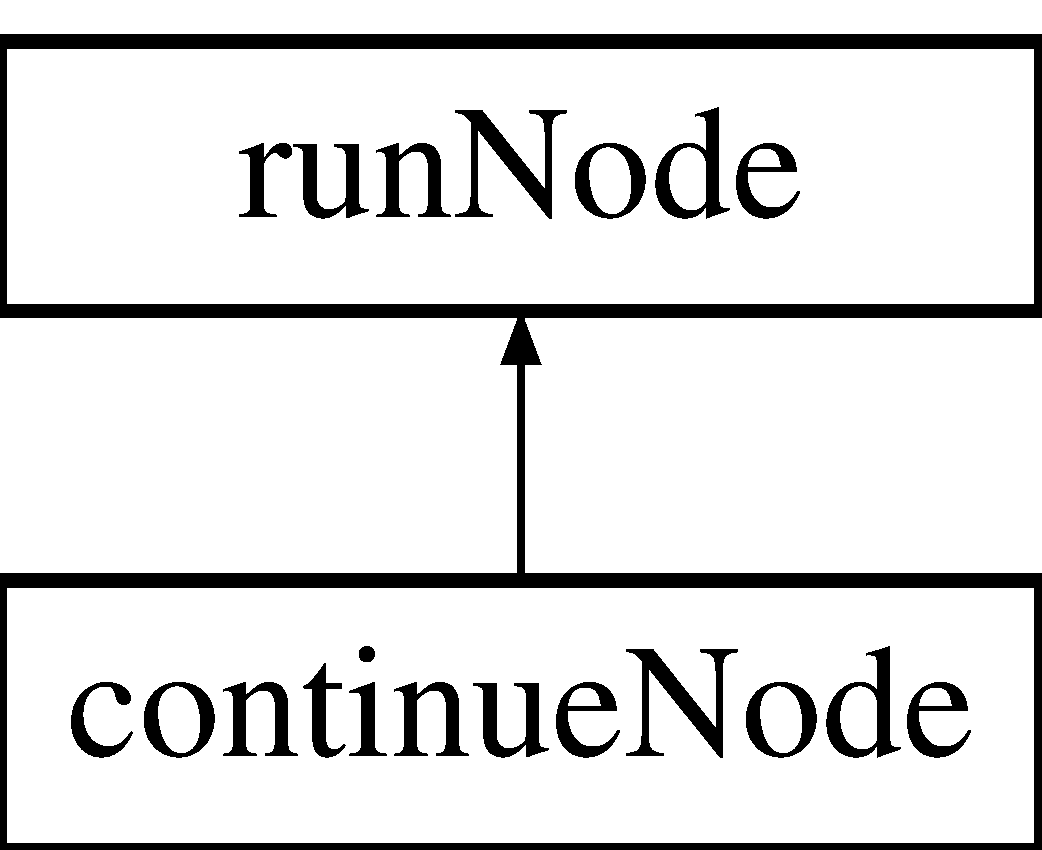
\includegraphics[height=2.000000cm]{classcontinueNode}
\end{center}
\end{figure}
\subsection*{Métodos públicos}
\begin{DoxyCompactItemize}
\item 
\hyperlink{classcontinueNode_ace21e3368be1423dbe879546c61f25f2}{continue\-Node} (int n=1)
\item 
void \hyperlink{classcontinueNode_afef4eca9866bfb614c779a5c9b02adc1}{run} ()
\end{DoxyCompactItemize}
\subsection*{Otros miembros heredados}


\subsection{Descripción detallada}
Nodo sentencia continue. 

Este nodo se utiliza para finalizar la iteración actual de un bloque de sentencias en una sentencia iterativa. Prosiguiendo así con la evaluación de la siguiente iteración.

Es posible especificar un valor que indica el número de sentencias iterativas que se saltarán.

Internamente se lanza una excepción (\begin{DoxySeeAlso}{Ver también}
\hyperlink{classcontinueException}{continue\-Exception}) que será atrapada por las sentencias iterativas. 
\end{DoxySeeAlso}


\subsection{Documentación del constructor y destructor}
\hypertarget{classcontinueNode_ace21e3368be1423dbe879546c61f25f2}{\index{continue\-Node@{continue\-Node}!continue\-Node@{continue\-Node}}
\index{continue\-Node@{continue\-Node}!continueNode@{continue\-Node}}
\subsubsection[{continue\-Node}]{\setlength{\rightskip}{0pt plus 5cm}continue\-Node\-::continue\-Node (
\begin{DoxyParamCaption}
\item[{int}]{n = {\ttfamily 1}}
\end{DoxyParamCaption}
)}}\label{classcontinueNode_ace21e3368be1423dbe879546c61f25f2}
Cosntructor de la clase 
\begin{DoxyParams}{Parámetros}
{\em n} & Entero que indica el número de sentencias iterativas anidadas que se saltarán \\
\hline
\end{DoxyParams}


\subsection{Documentación de las funciones miembro}
\hypertarget{classcontinueNode_afef4eca9866bfb614c779a5c9b02adc1}{\index{continue\-Node@{continue\-Node}!run@{run}}
\index{run@{run}!continueNode@{continue\-Node}}
\subsubsection[{run}]{\setlength{\rightskip}{0pt plus 5cm}void continue\-Node\-::run (
\begin{DoxyParamCaption}
{}
\end{DoxyParamCaption}
)\hspace{0.3cm}{\ttfamily [virtual]}}}\label{classcontinueNode_afef4eca9866bfb614c779a5c9b02adc1}
Método que lleva a cabo la ejecución del nodo. Lanza una excepción continue que obliga a las sentencias iterativas a seguir con la siguiente iteración. 

Implementa \hyperlink{classrunNode_a83c10df8148829b08e04153c93d69eec}{run\-Node}.



La documentación para esta clase fue generada a partir de los siguientes ficheros\-:\begin{DoxyCompactItemize}
\item 
trunk/src/run/stmts/\hyperlink{loopStmtNode_8h}{loop\-Stmt\-Node.\-h}\item 
trunk/src/run/stmts/loop\-Stmt\-Node.\-cpp\end{DoxyCompactItemize}

\hypertarget{classdateNode}{\section{Referencia de la Clase date\-Node}
\label{classdateNode}\index{date\-Node@{date\-Node}}
}


Nodo función fecha.  




{\ttfamily \#include $<$date\-Op\-Node.\-h$>$}

Diagrama de herencias de date\-Node\begin{figure}[H]
\begin{center}
\leavevmode
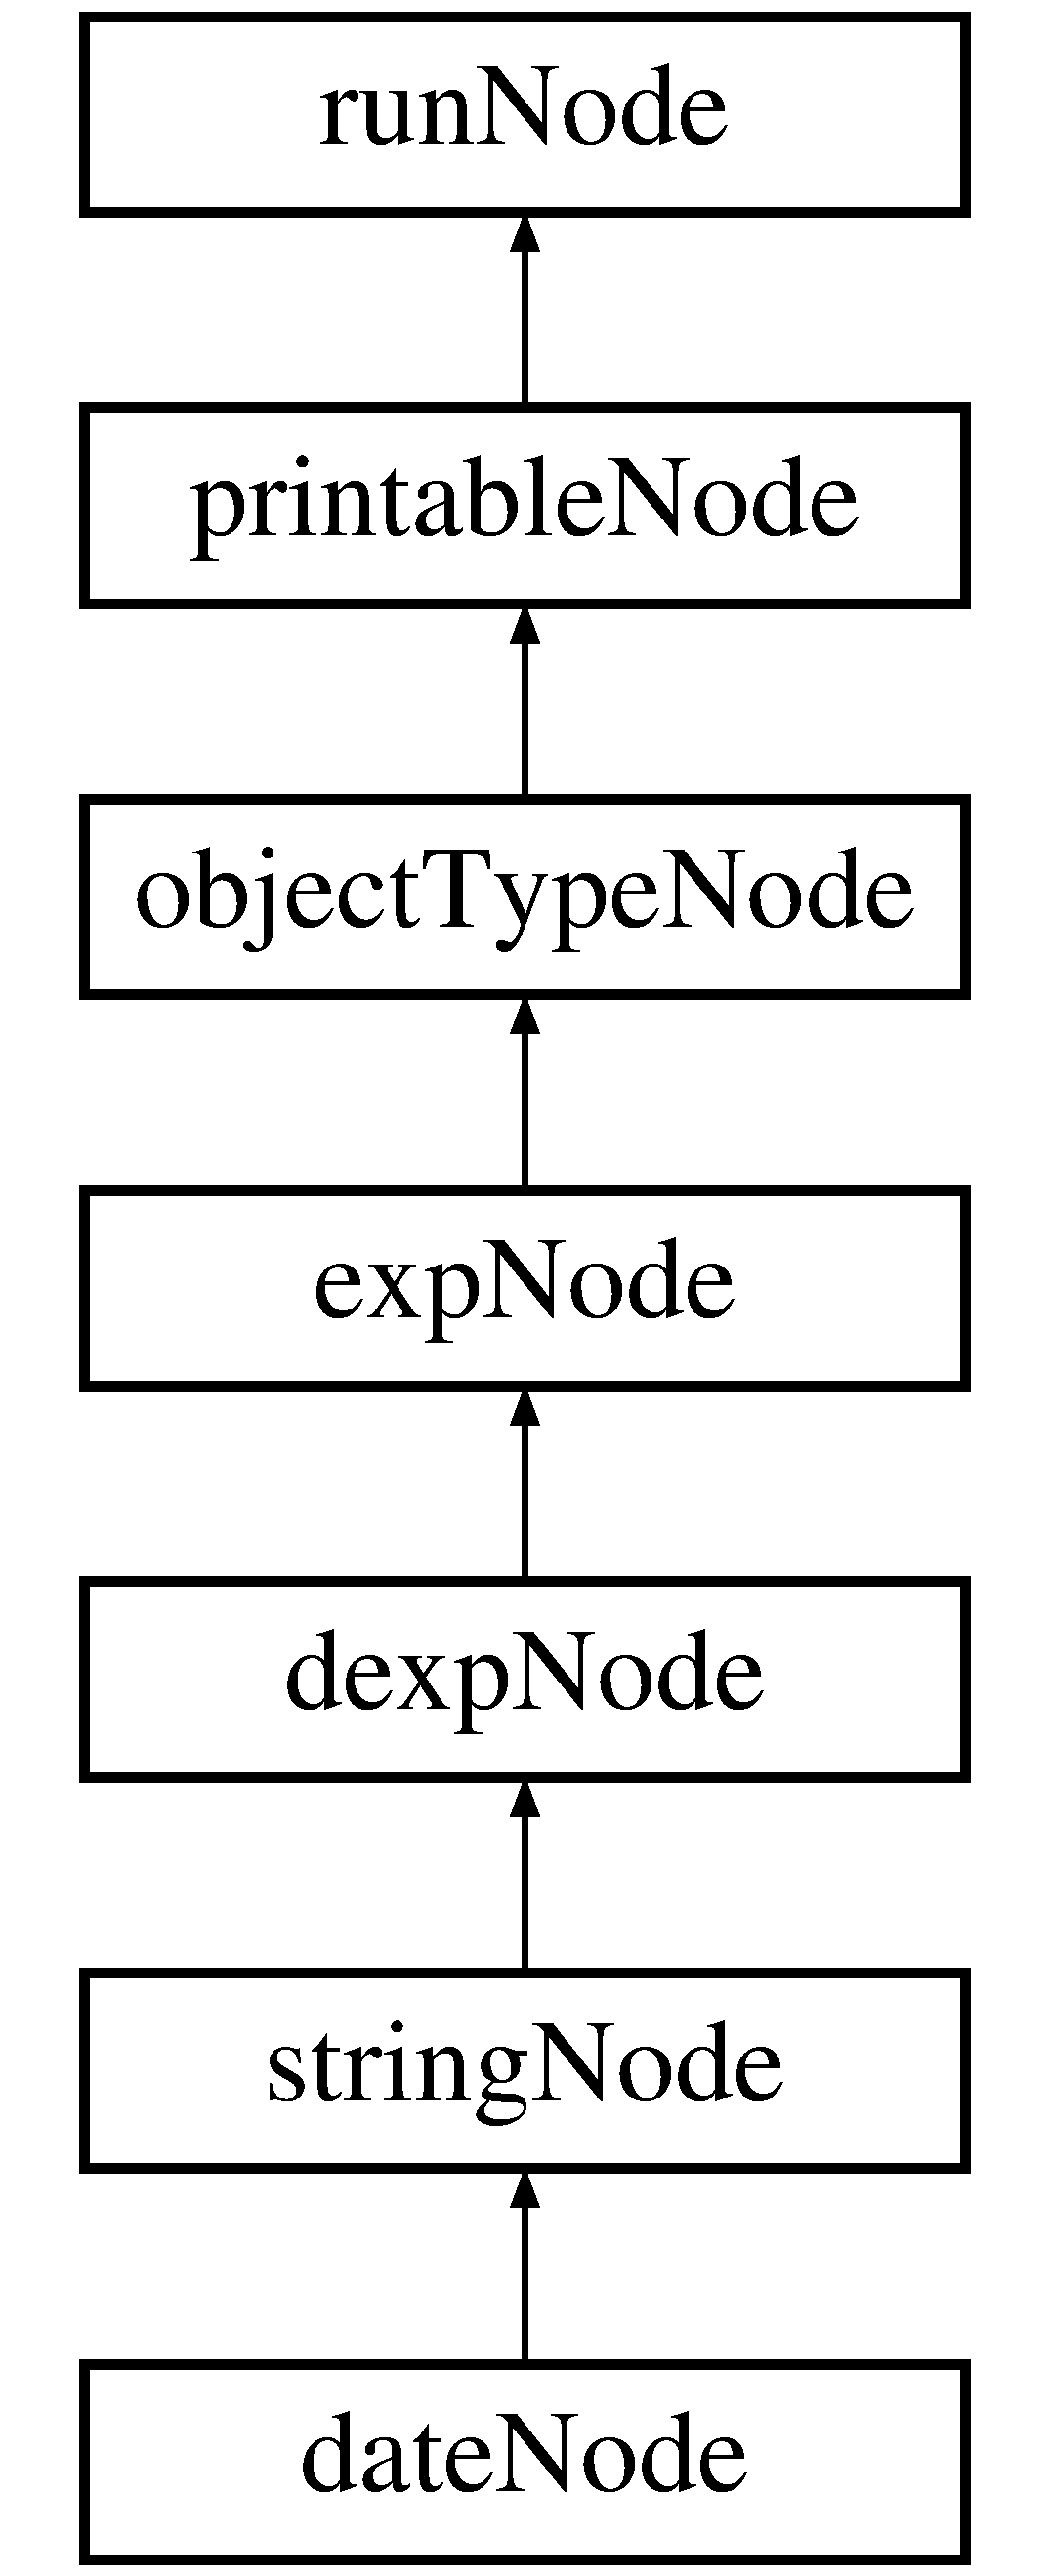
\includegraphics[height=7.000000cm]{classdateNode}
\end{center}
\end{figure}
\subsection*{Métodos públicos}
\begin{DoxyCompactItemize}
\item 
\hyperlink{classdateNode_a3227bbfae0a0bdf38bc312a525b4216c}{date\-Node} (\hyperlink{classrunNode}{run\-Node} $\ast$str, \hyperlink{classrunNode}{run\-Node} $\ast$timestamp=N\-U\-L\-L)
\item 
void \hyperlink{classdateNode_ad13a252816fd28e65c027ad49d8c3976}{run} ()
\end{DoxyCompactItemize}
\subsection*{Otros miembros heredados}


\subsection{Descripción detallada}
Nodo función fecha. 

Este nodo genera una caneda que se corresponde a una fecha dada según un formato y una marca de tiempo.

Para la cadena de formato se utiliza las siguentes directivas\-:
\begin{DoxyItemize}
\item d\-: Día del mes con dos dígitos.
\item j\-: Día del mes sin ceros iniciales.
\item l\-: Día de la semana de forma alfabética completa.
\item D\-: Día de la semana de forma alfabética y con tres letras.
\item w\-: Día de la semana de forma numérica (0-\/domingo,6-\/sábado).
\item z\-: Día del año de forma numérica.
\item F\-: Mes de forma alfabética.
\item m\-: Mes de forma numérica con dos dígitos.
\item n\-: Mes de forma numérica sin ceros iniciales.
\item M\-: Mes de forma alfabética con tres letras.
\item Y\-: Año con cuatro dígitos.
\item y\-: Año con dos dígitos.
\item a\-: Periodo del día (am/pm) en minúsculas.
\item A\-: Periodo del día (am/pm) en mayúsculas.
\item g\-: Hora en formato 12h sin ceros iniciales.
\item G\-: Hora en formato 24h sin ceros iniciales.
\item h\-: Hora en formato 12h con dos dígitos.
\item H\-: Hora en formato 24h con dos dígitos.
\item i\-: Minutos con dos dígitos.
\item U\-: Segundos desde la Época Unix (1 de Enero del 1970 00\-:00\-:00 G\-M\-T).
\item \%\%\-: Carácter \%. 
\end{DoxyItemize}

\subsection{Documentación del constructor y destructor}
\hypertarget{classdateNode_a3227bbfae0a0bdf38bc312a525b4216c}{\index{date\-Node@{date\-Node}!date\-Node@{date\-Node}}
\index{date\-Node@{date\-Node}!dateNode@{date\-Node}}
\subsubsection[{date\-Node}]{\setlength{\rightskip}{0pt plus 5cm}date\-Node\-::date\-Node (
\begin{DoxyParamCaption}
\item[{{\bf run\-Node} $\ast$}]{str, }
\item[{{\bf run\-Node} $\ast$}]{timestamp = {\ttfamily NULL}}
\end{DoxyParamCaption}
)}}\label{classdateNode_a3227bbfae0a0bdf38bc312a525b4216c}
Constructor de la clase. 
\begin{DoxyParams}{Parámetros}
{\em str} & Nodo que representa la cadena de formato \\
\hline
{\em timestamp} & Nodo que respresenta la marca de tiempo. Si no se da se toma la marca de tiempo actual. \\
\hline
\end{DoxyParams}


\subsection{Documentación de las funciones miembro}
\hypertarget{classdateNode_ad13a252816fd28e65c027ad49d8c3976}{\index{date\-Node@{date\-Node}!run@{run}}
\index{run@{run}!dateNode@{date\-Node}}
\subsubsection[{run}]{\setlength{\rightskip}{0pt plus 5cm}void date\-Node\-::run (
\begin{DoxyParamCaption}
{}
\end{DoxyParamCaption}
)\hspace{0.3cm}{\ttfamily [virtual]}}}\label{classdateNode_ad13a252816fd28e65c027ad49d8c3976}
Método que lleva a cabo la ejecución del nodo. Toma como valor una cadena determinada por la cadena de formato y la marca de tiempo. 

Implementa \hyperlink{classrunNode_a83c10df8148829b08e04153c93d69eec}{run\-Node}.



La documentación para esta clase fue generada a partir de los siguientes ficheros\-:\begin{DoxyCompactItemize}
\item 
trunk/src/run/operators/\hyperlink{dateOpNode_8h}{date\-Op\-Node.\-h}\item 
trunk/src/run/operators/date\-Op\-Node.\-cpp\end{DoxyCompactItemize}

\hypertarget{classdatInfoNode}{\section{Referencia de la Clase dat\-Info\-Node}
\label{classdatInfoNode}\index{dat\-Info\-Node@{dat\-Info\-Node}}
}


Nodo información sobre dato.  




{\ttfamily \#include $<$stmt\-Node.\-h$>$}

Diagrama de herencias de dat\-Info\-Node\begin{figure}[H]
\begin{center}
\leavevmode
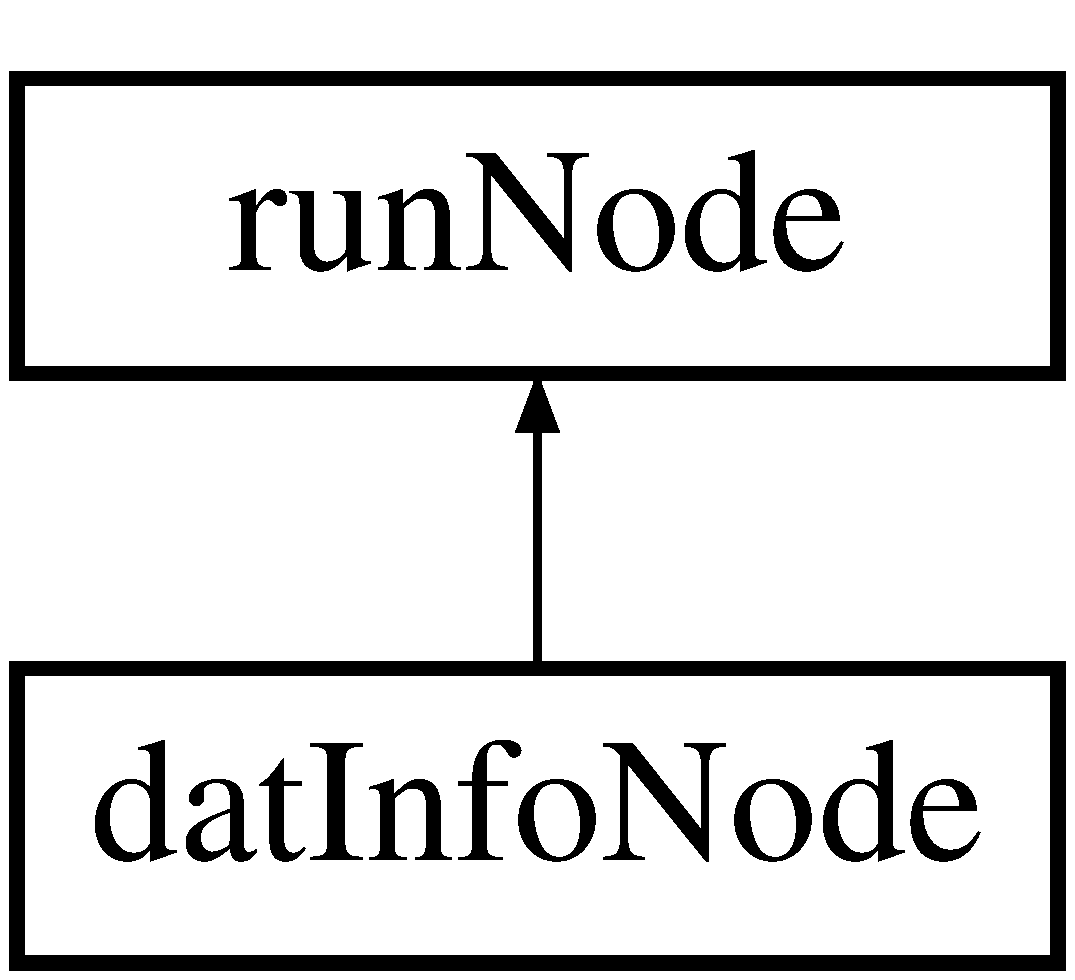
\includegraphics[height=2.000000cm]{classdatInfoNode}
\end{center}
\end{figure}
\subsection*{Métodos públicos}
\begin{DoxyCompactItemize}
\item 
\hyperlink{classdatInfoNode_a40adb798bbeb6f9fa4fdcfbd21086bea}{dat\-Info\-Node} (\hyperlink{classrunNode}{run\-Node} $\ast$node)
\item 
void \hyperlink{classdatInfoNode_a681d40c5a8d3b567da3c167a1c701e59}{run} ()
\end{DoxyCompactItemize}
\subsection*{Otros miembros heredados}


\subsection{Descripción detallada}
Nodo información sobre dato. 

La ejecución de este nodo consiste en imprimir datos internos del nodo tales como la posición de memoria que ocupa, el tipo o el número de referencias. 

\subsection{Documentación del constructor y destructor}
\hypertarget{classdatInfoNode_a40adb798bbeb6f9fa4fdcfbd21086bea}{\index{dat\-Info\-Node@{dat\-Info\-Node}!dat\-Info\-Node@{dat\-Info\-Node}}
\index{dat\-Info\-Node@{dat\-Info\-Node}!datInfoNode@{dat\-Info\-Node}}
\subsubsection[{dat\-Info\-Node}]{\setlength{\rightskip}{0pt plus 5cm}dat\-Info\-Node\-::dat\-Info\-Node (
\begin{DoxyParamCaption}
\item[{{\bf run\-Node} $\ast$}]{node}
\end{DoxyParamCaption}
)}}\label{classdatInfoNode_a40adb798bbeb6f9fa4fdcfbd21086bea}
Constructor de clase 
\begin{DoxyParams}{Parámetros}
{\em node} & Nodo que será consultado \\
\hline
\end{DoxyParams}


\subsection{Documentación de las funciones miembro}
\hypertarget{classdatInfoNode_a681d40c5a8d3b567da3c167a1c701e59}{\index{dat\-Info\-Node@{dat\-Info\-Node}!run@{run}}
\index{run@{run}!datInfoNode@{dat\-Info\-Node}}
\subsubsection[{run}]{\setlength{\rightskip}{0pt plus 5cm}void dat\-Info\-Node\-::run (
\begin{DoxyParamCaption}
{}
\end{DoxyParamCaption}
)\hspace{0.3cm}{\ttfamily [virtual]}}}\label{classdatInfoNode_a681d40c5a8d3b567da3c167a1c701e59}
Ejecución del nodo. Imprime en la salida entándar el tipo del nodo, identificador asociado si tuviera, número de elementos en caso de ser compuesto, el valor y el número de referencias 

Implementa \hyperlink{classrunNode_a83c10df8148829b08e04153c93d69eec}{run\-Node}.



La documentación para esta clase fue generada a partir de los siguientes ficheros\-:\begin{DoxyCompactItemize}
\item 
trunk/src/run/stmts/\hyperlink{stmtNode_8h}{stmt\-Node.\-h}\item 
trunk/src/run/stmts/stmt\-Node.\-cpp\end{DoxyCompactItemize}

\hypertarget{classdecasigNode}{\section{Referencia de la Clase decasig\-Node}
\label{classdecasigNode}\index{decasig\-Node@{decasig\-Node}}
}


Nodo operador decremento y asignación.  




{\ttfamily \#include $<$arith\-Op\-Node.\-h$>$}

Diagrama de herencias de decasig\-Node\begin{figure}[H]
\begin{center}
\leavevmode
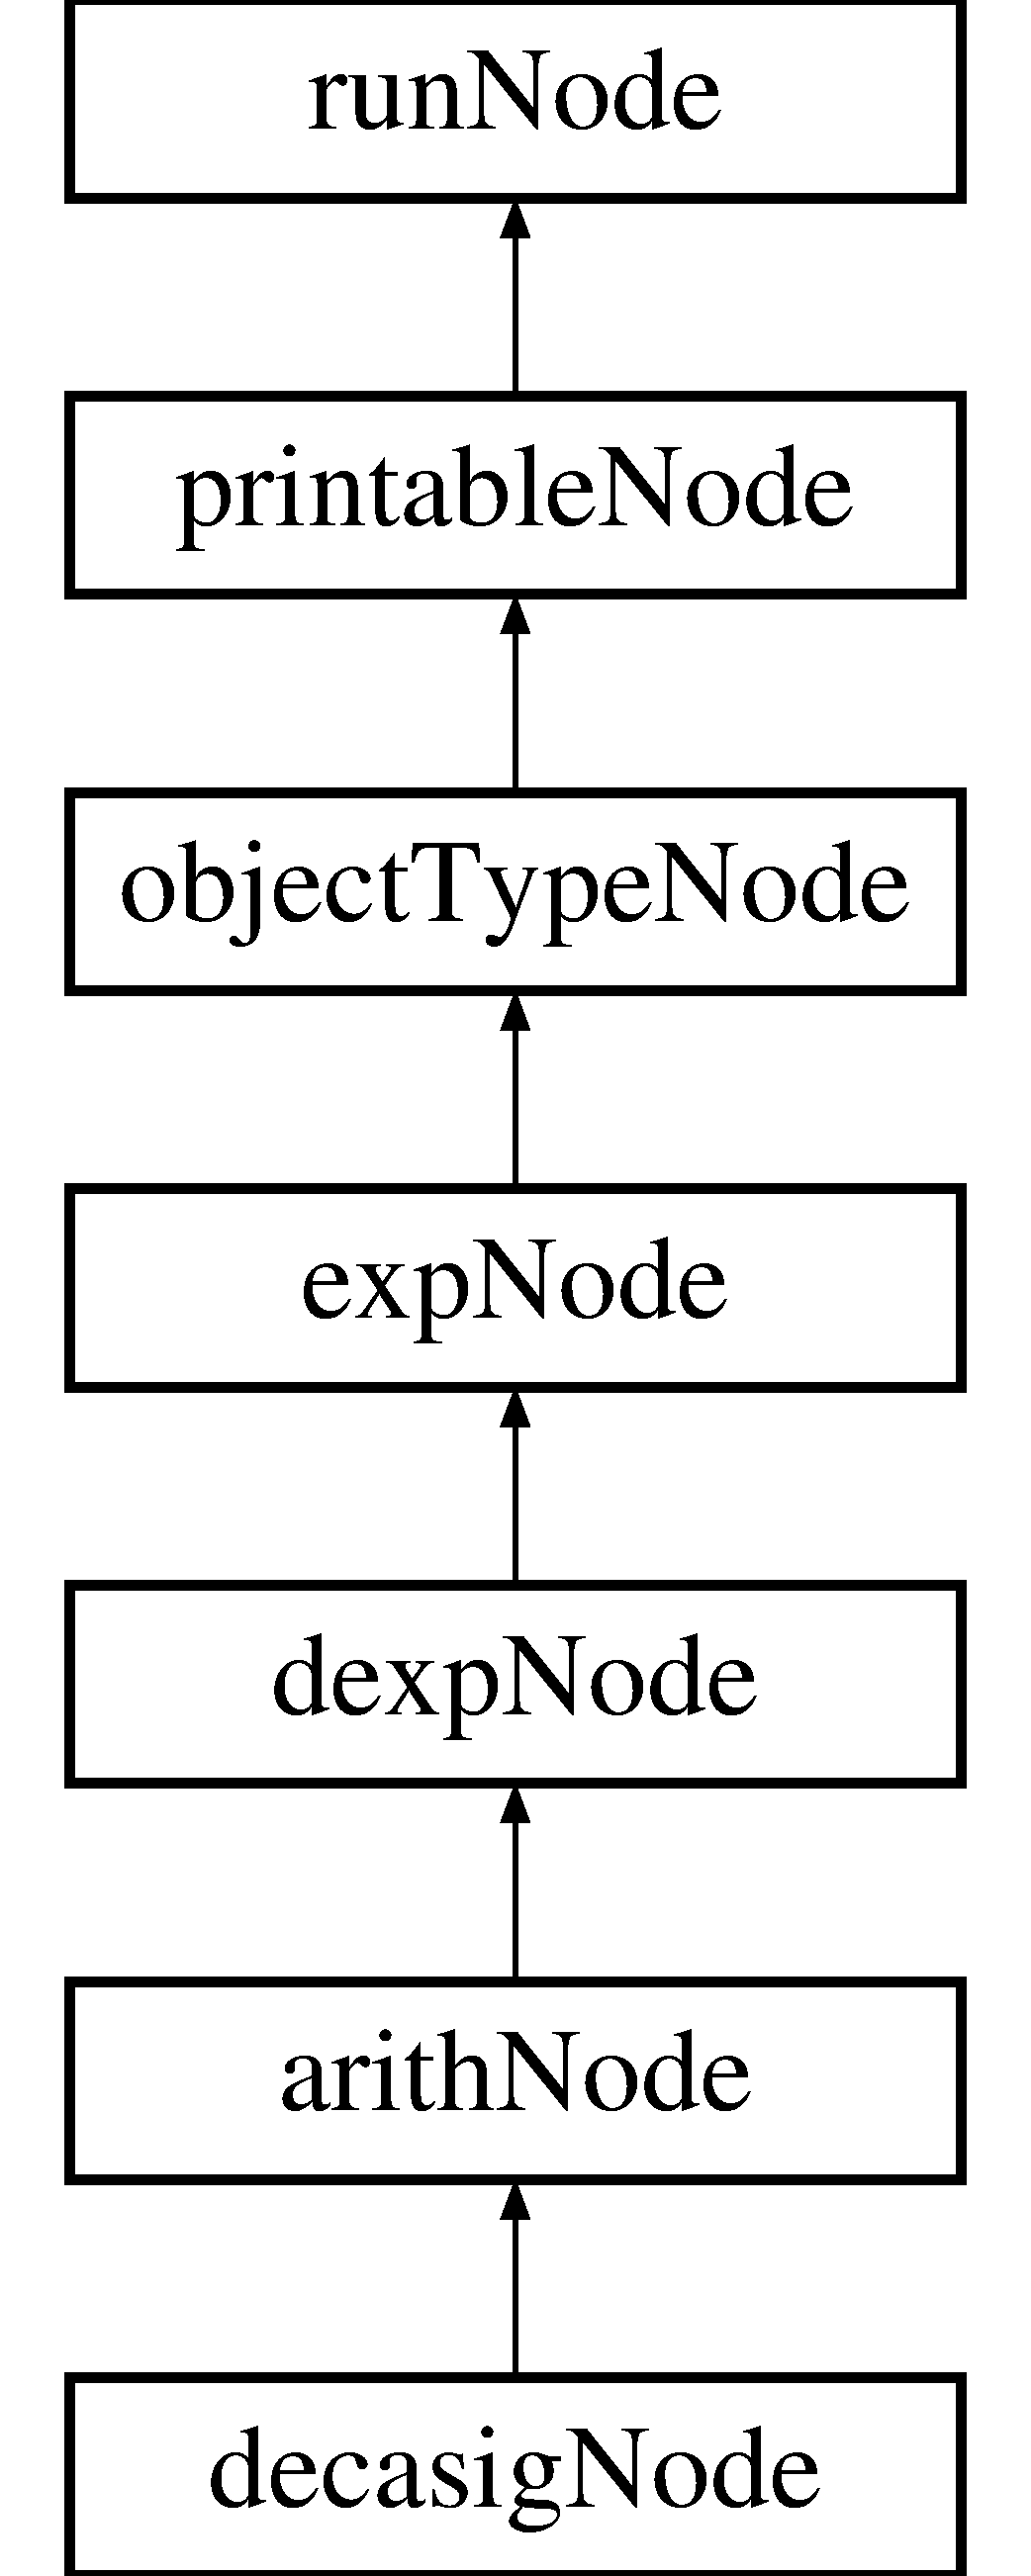
\includegraphics[height=7.000000cm]{classdecasigNode}
\end{center}
\end{figure}
\subsection*{Métodos públicos}
\begin{DoxyCompactItemize}
\item 
\hyperlink{classdecasigNode_aac7063a27fc37eaae22f4d66266bf800}{decasig\-Node} (\hyperlink{classrunNode}{run\-Node} $\ast$node)
\item 
void \hyperlink{classdecasigNode_ac45f48e8d9866816c2efae4eed38d833}{run} ()
\end{DoxyCompactItemize}
\subsection*{Otros miembros heredados}


\subsection{Descripción detallada}
Nodo operador decremento y asignación. 

Este nodo implementa la operación decremento y asignación. Se lleva a cabo el incremento del nodo asociado, luego el nuevo resultado se utiliza como valor del operador.

El resultado de evaluar la expresión es un valor aritmético correspondiente al decremento. 

\subsection{Documentación del constructor y destructor}
\hypertarget{classdecasigNode_aac7063a27fc37eaae22f4d66266bf800}{\index{decasig\-Node@{decasig\-Node}!decasig\-Node@{decasig\-Node}}
\index{decasig\-Node@{decasig\-Node}!decasigNode@{decasig\-Node}}
\subsubsection[{decasig\-Node}]{\setlength{\rightskip}{0pt plus 5cm}decasig\-Node\-::decasig\-Node (
\begin{DoxyParamCaption}
\item[{{\bf run\-Node} $\ast$}]{node}
\end{DoxyParamCaption}
)}}\label{classdecasigNode_aac7063a27fc37eaae22f4d66266bf800}
Constructor de la clase. Asocia el nodo operador a un nodo. 
\begin{DoxyParams}{Parámetros}
{\em node} & Nodo operando. \\
\hline
\end{DoxyParams}


\subsection{Documentación de las funciones miembro}
\hypertarget{classdecasigNode_ac45f48e8d9866816c2efae4eed38d833}{\index{decasig\-Node@{decasig\-Node}!run@{run}}
\index{run@{run}!decasigNode@{decasig\-Node}}
\subsubsection[{run}]{\setlength{\rightskip}{0pt plus 5cm}void decasig\-Node\-::run (
\begin{DoxyParamCaption}
{}
\end{DoxyParamCaption}
)\hspace{0.3cm}{\ttfamily [virtual]}}}\label{classdecasigNode_ac45f48e8d9866816c2efae4eed38d833}
Método que ejecuta el nodo. Procede a incrementar el valor del nodo operando. Luego asocia el resultado del incremento como valor interno del operador. 

Implementa \hyperlink{classrunNode_a83c10df8148829b08e04153c93d69eec}{run\-Node}.



La documentación para esta clase fue generada a partir de los siguientes ficheros\-:\begin{DoxyCompactItemize}
\item 
trunk/src/run/operators/\hyperlink{arithOpNode_8h}{arith\-Op\-Node.\-h}\item 
trunk/src/run/operators/arith\-Op\-Node.\-cpp\end{DoxyCompactItemize}

\hypertarget{classdexpNode}{\section{Referencia de la Clase dexp\-Node}
\label{classdexpNode}\index{dexp\-Node@{dexp\-Node}}
}


Nodo expresión de tipo definido.  




{\ttfamily \#include $<$exp\-Node.\-h$>$}

Diagrama de herencias de dexp\-Node\begin{figure}[H]
\begin{center}
\leavevmode
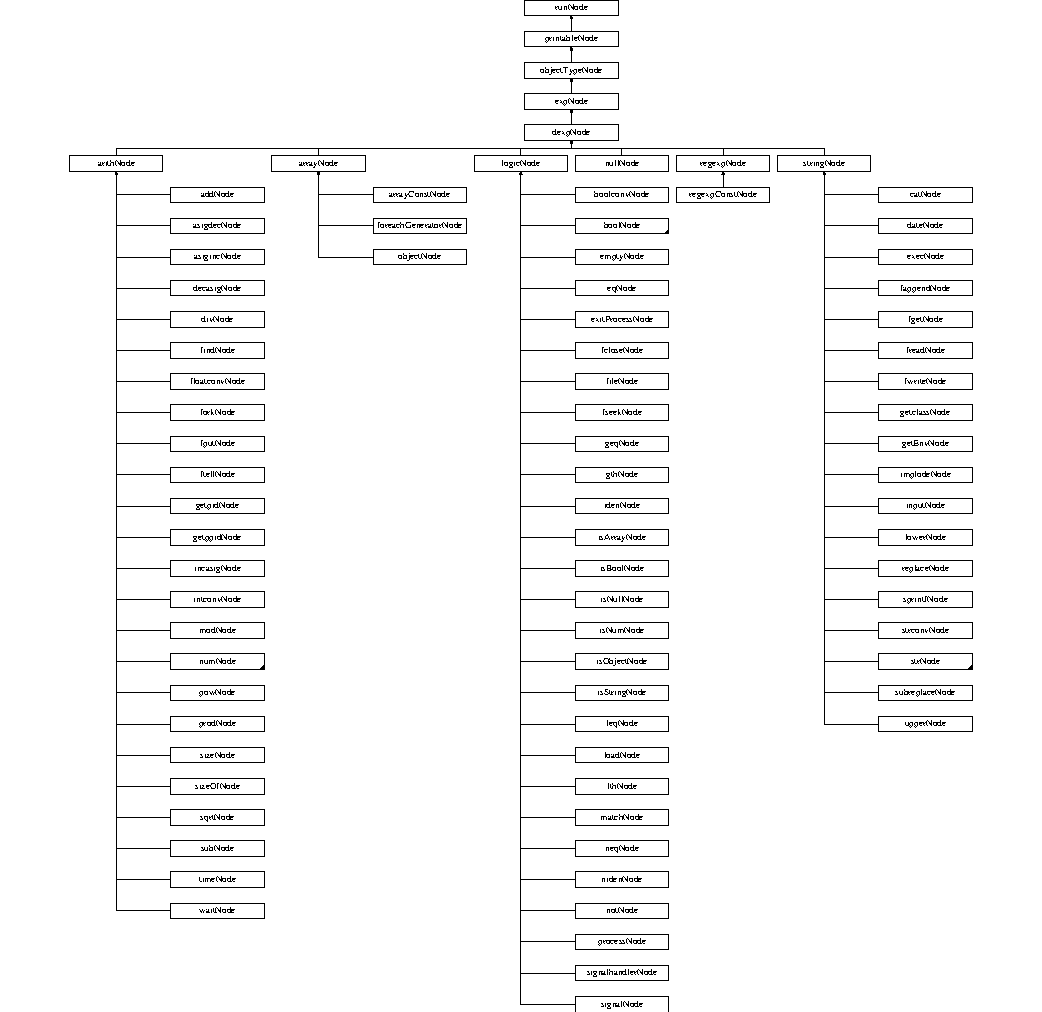
\includegraphics[height=12.000000cm]{classdexpNode}
\end{center}
\end{figure}
\subsection*{Métodos públicos}
\begin{DoxyCompactItemize}
\item 
virtual bool \hyperlink{classdexpNode_a18781e07cc3390c04b6905249755ccc8}{boolvalue} () const 
\item 
virtual num \hyperlink{classdexpNode_ae2d3bfed7e6ebd5e96ddcefaa230c3d2}{numvalue} () const 
\item 
virtual string \hyperlink{classdexpNode_adf74f4f848f7ec7c3c2ada1aa3bdc66d}{strvalue} () const 
\end{DoxyCompactItemize}
\subsection*{Otros miembros heredados}


\subsection{Descripción detallada}
Nodo expresión de tipo definido. 

Los nodos de expresión de tipo definido tienen un valor o conjunto de valores asociados. Estos valores son de un tipo concreto, conocido y definido.

Toda expresión definida podrá realizar una conversión de su valor interno a los tipos booleano, numérico y cadena de caracteres.

Estos nodos se dividen en dos grupos\-:


\begin{DoxyItemize}
\item Nodos tipos\-: Definen los tipos de datos básicos\-: booleanos, numéricos, cadenas, arrays ...
\end{DoxyItemize}

-\/\-Nodos operadores definidos\-: Definen operaciones cuyo tipo de valor es conocido. Por ejemplo\-: la operación suma tiene un valor numérico asociado. la comparación de igualdad un valor booleano; 

\subsection{Documentación de las funciones miembro}
\hypertarget{classdexpNode_a18781e07cc3390c04b6905249755ccc8}{\index{dexp\-Node@{dexp\-Node}!boolvalue@{boolvalue}}
\index{boolvalue@{boolvalue}!dexpNode@{dexp\-Node}}
\subsubsection[{boolvalue}]{\setlength{\rightskip}{0pt plus 5cm}bool dexp\-Node\-::boolvalue (
\begin{DoxyParamCaption}
{}
\end{DoxyParamCaption}
) const\hspace{0.3cm}{\ttfamily [virtual]}}}\label{classdexpNode_a18781e07cc3390c04b6905249755ccc8}
Obtiene el valor booleano del nodo. \begin{DoxyReturn}{Devuelve}
Booleano que representa el valor del nodo. 
\end{DoxyReturn}


Reimplementado en \hyperlink{classregexpNode_a10a587695cb42fa6f9d867e05e26068f}{regexp\-Node}, \hyperlink{classarrayNode_af18a8d4f5e369713a01387bad022db72}{array\-Node}, \hyperlink{classstringNode_ae1fe6ea419679a0a0402beb47fabcea2}{string\-Node}, \hyperlink{classarithNode_a7f3634eba193b245af5e3ba8081c017b}{arith\-Node} y \hyperlink{classlogicNode_a802078f6b9ec9f96e01c91ac1704099b}{logic\-Node}.

\hypertarget{classdexpNode_ae2d3bfed7e6ebd5e96ddcefaa230c3d2}{\index{dexp\-Node@{dexp\-Node}!numvalue@{numvalue}}
\index{numvalue@{numvalue}!dexpNode@{dexp\-Node}}
\subsubsection[{numvalue}]{\setlength{\rightskip}{0pt plus 5cm}num dexp\-Node\-::numvalue (
\begin{DoxyParamCaption}
{}
\end{DoxyParamCaption}
) const\hspace{0.3cm}{\ttfamily [virtual]}}}\label{classdexpNode_ae2d3bfed7e6ebd5e96ddcefaa230c3d2}
Obtiene el valor numérico del nodo. \begin{DoxyReturn}{Devuelve}
Numérico que representa el valor del nodo. 
\end{DoxyReturn}


Reimplementado en \hyperlink{classregexpNode_a6d6e4d51eaedec3def49747e4da3b03b}{regexp\-Node}, \hyperlink{classarrayNode_a8a862493dfcab500edd9acf4f4c55348}{array\-Node}, \hyperlink{classstringNode_ae66cab7ddc65acc8541d88baaebf47fb}{string\-Node}, \hyperlink{classarithNode_a3914e65779e61750f1ffd528deabd120}{arith\-Node} y \hyperlink{classlogicNode_a8fbc68e3cd354745e0e34ab4027bb8cc}{logic\-Node}.

\hypertarget{classdexpNode_adf74f4f848f7ec7c3c2ada1aa3bdc66d}{\index{dexp\-Node@{dexp\-Node}!strvalue@{strvalue}}
\index{strvalue@{strvalue}!dexpNode@{dexp\-Node}}
\subsubsection[{strvalue}]{\setlength{\rightskip}{0pt plus 5cm}string dexp\-Node\-::strvalue (
\begin{DoxyParamCaption}
{}
\end{DoxyParamCaption}
) const\hspace{0.3cm}{\ttfamily [virtual]}}}\label{classdexpNode_adf74f4f848f7ec7c3c2ada1aa3bdc66d}
Obtiene el valor cadena de caracteres del nodo. \begin{DoxyReturn}{Devuelve}
Cadena de caracteres que representa el valor del nodo. 
\end{DoxyReturn}


Reimplementado en \hyperlink{classregexpNode_a223644545a3ec0258c6083fa8686a3cb}{regexp\-Node}, \hyperlink{classarrayNode_a3e5771d0cf67476bfe19683d504327d1}{array\-Node}, \hyperlink{classstringNode_adbc47d59c690cbd5a231d9a44384e1ba}{string\-Node}, \hyperlink{classarithNode_a01f251d6cdc918309873c7443c694510}{arith\-Node} y \hyperlink{classlogicNode_a5a5daf0f2b1295126998ac3a9fe0cc77}{logic\-Node}.



La documentación para esta clase fue generada a partir de los siguientes ficheros\-:\begin{DoxyCompactItemize}
\item 
trunk/src/run/tree/\hyperlink{expNode_8h}{exp\-Node.\-h}\item 
trunk/src/run/tree/exp\-Node.\-cpp\end{DoxyCompactItemize}

\hypertarget{classdivNode}{\section{Referencia de la Clase div\-Node}
\label{classdivNode}\index{div\-Node@{div\-Node}}
}


Nodo operador división.  




{\ttfamily \#include $<$arith\-Op\-Node.\-h$>$}

Diagrama de herencias de div\-Node\begin{figure}[H]
\begin{center}
\leavevmode
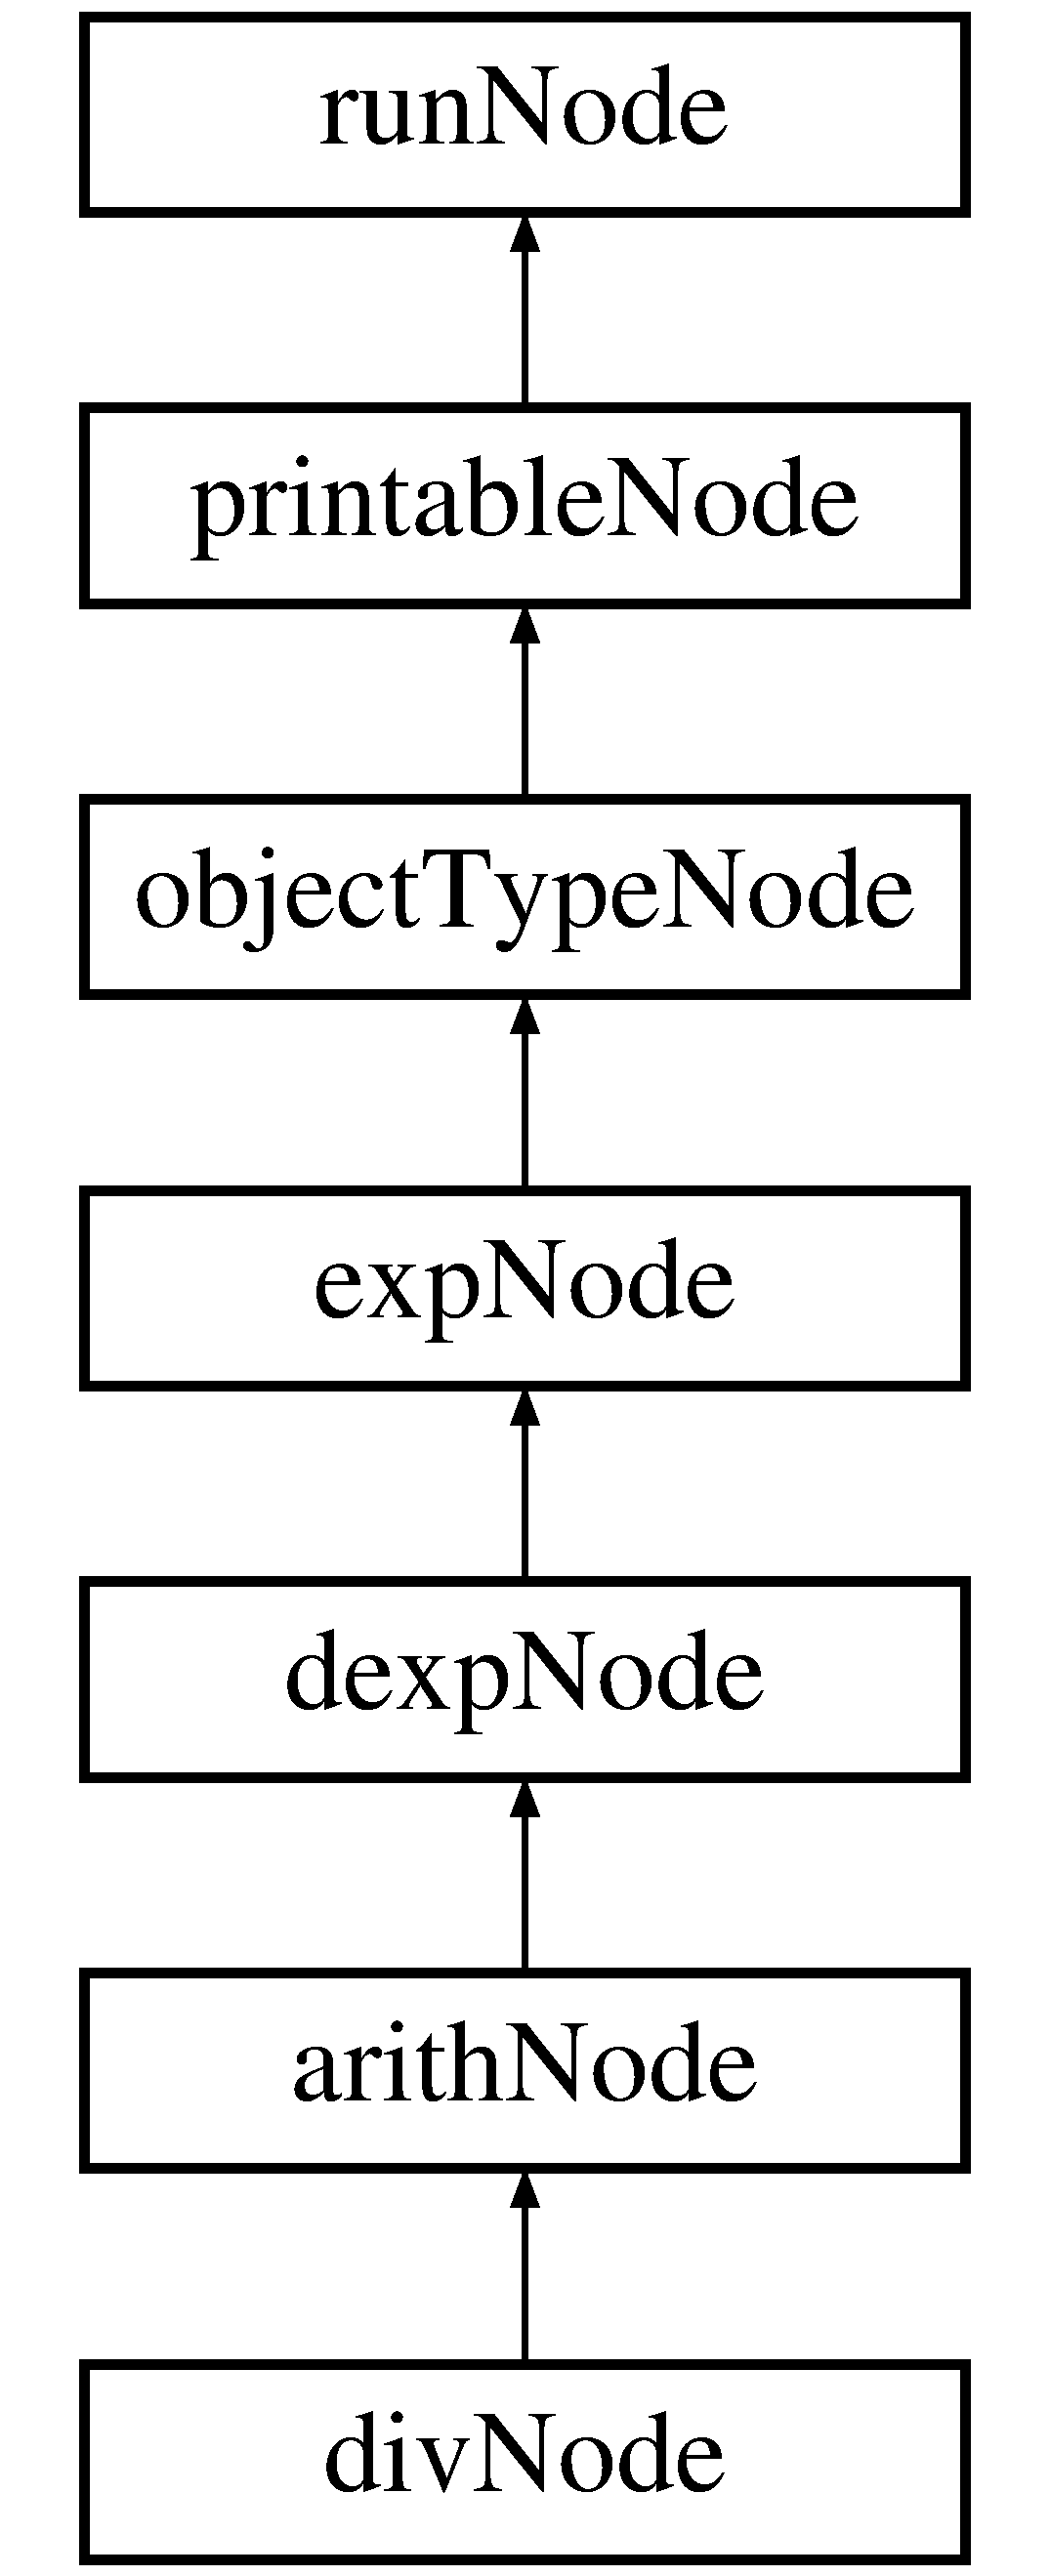
\includegraphics[height=7.000000cm]{classdivNode}
\end{center}
\end{figure}
\subsection*{Métodos públicos}
\begin{DoxyCompactItemize}
\item 
\hyperlink{classdivNode_aaf5444aa1b13960627066006f1a1ed5c}{div\-Node} (\hyperlink{classrunNode}{run\-Node} $\ast$node1, \hyperlink{classrunNode}{run\-Node} $\ast$node2)
\item 
void \hyperlink{classdivNode_a56aa027a86b596362a5741bed8b8eb51}{run} ()
\end{DoxyCompactItemize}
\subsection*{Métodos públicos estáticos}
\begin{DoxyCompactItemize}
\item 
static num \hyperlink{classdivNode_a6ecab675baf7410067278bf0a1734f0e}{do\-\_\-div} (\hyperlink{classrunNode}{run\-Node} $\ast$op1, \hyperlink{classrunNode}{run\-Node} $\ast$op2)
\end{DoxyCompactItemize}
\subsection*{Otros miembros heredados}


\subsection{Descripción detallada}
Nodo operador división. 

Este nodo implementa la operación división sobre dos nodos asociados.

Si algún nodo es de tipo no aritmético fuerza la conversión a un tipo aritmético para realizar la operación

El resultado de evaluar la expresión es un valor aritmético. 

\subsection{Documentación del constructor y destructor}
\hypertarget{classdivNode_aaf5444aa1b13960627066006f1a1ed5c}{\index{div\-Node@{div\-Node}!div\-Node@{div\-Node}}
\index{div\-Node@{div\-Node}!divNode@{div\-Node}}
\subsubsection[{div\-Node}]{\setlength{\rightskip}{0pt plus 5cm}div\-Node\-::div\-Node (
\begin{DoxyParamCaption}
\item[{{\bf run\-Node} $\ast$}]{node1, }
\item[{{\bf run\-Node} $\ast$}]{node2}
\end{DoxyParamCaption}
)}}\label{classdivNode_aaf5444aa1b13960627066006f1a1ed5c}
Constructor de la clase. Asocia el nodo operador a dos nodos aritméticos. 
\begin{DoxyParams}{Parámetros}
{\em node1} & Primer nodo operando. \\
\hline
{\em node2} & Segundo nodo operando. \\
\hline
\end{DoxyParams}


\subsection{Documentación de las funciones miembro}
\hypertarget{classdivNode_a6ecab675baf7410067278bf0a1734f0e}{\index{div\-Node@{div\-Node}!do\-\_\-div@{do\-\_\-div}}
\index{do\-\_\-div@{do\-\_\-div}!divNode@{div\-Node}}
\subsubsection[{do\-\_\-div}]{\setlength{\rightskip}{0pt plus 5cm}num div\-Node\-::do\-\_\-div (
\begin{DoxyParamCaption}
\item[{{\bf run\-Node} $\ast$}]{op1, }
\item[{{\bf run\-Node} $\ast$}]{op2}
\end{DoxyParamCaption}
)\hspace{0.3cm}{\ttfamily [static]}}}\label{classdivNode_a6ecab675baf7410067278bf0a1734f0e}
Ejecuta la operación división sobre dos nodos dados 
\begin{DoxyParams}{Parámetros}
{\em op1} & Primer nodo operando. \\
\hline
{\em op2} & Segundo nodo operando. \\
\hline
\end{DoxyParams}
\begin{DoxyReturn}{Devuelve}
Valor de la operación. 
\end{DoxyReturn}
\hypertarget{classdivNode_a56aa027a86b596362a5741bed8b8eb51}{\index{div\-Node@{div\-Node}!run@{run}}
\index{run@{run}!divNode@{div\-Node}}
\subsubsection[{run}]{\setlength{\rightskip}{0pt plus 5cm}void div\-Node\-::run (
\begin{DoxyParamCaption}
{}
\end{DoxyParamCaption}
)\hspace{0.3cm}{\ttfamily [virtual]}}}\label{classdivNode_a56aa027a86b596362a5741bed8b8eb51}
Método que ejecuta el nodo. Procede a la ejecución de los nodos asociados. Luego obtiene el valor aritmético del nodo mediante la operación producto entre el valor numérico de los dos nodos. 

Implementa \hyperlink{classrunNode_a83c10df8148829b08e04153c93d69eec}{run\-Node}.



La documentación para esta clase fue generada a partir de los siguientes ficheros\-:\begin{DoxyCompactItemize}
\item 
trunk/src/run/operators/\hyperlink{arithOpNode_8h}{arith\-Op\-Node.\-h}\item 
trunk/src/run/operators/arith\-Op\-Node.\-cpp\end{DoxyCompactItemize}

\hypertarget{classdowhileNode}{\section{Referencia de la Clase dowhile\-Node}
\label{classdowhileNode}\index{dowhile\-Node@{dowhile\-Node}}
}


Nodo sentencia do..while.  




{\ttfamily \#include $<$loop\-Stmt\-Node.\-h$>$}

Diagrama de herencias de dowhile\-Node\begin{figure}[H]
\begin{center}
\leavevmode
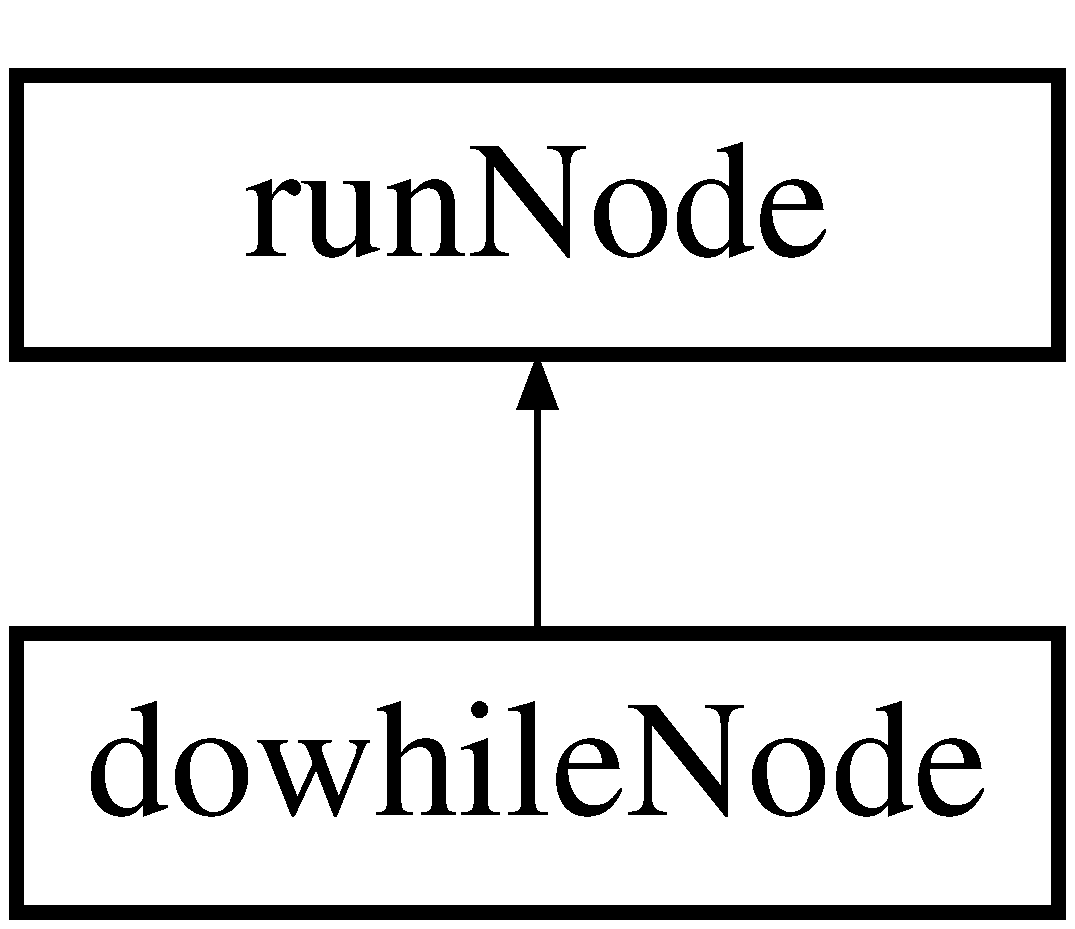
\includegraphics[height=2.000000cm]{classdowhileNode}
\end{center}
\end{figure}
\subsection*{Métodos públicos}
\begin{DoxyCompactItemize}
\item 
\hyperlink{classdowhileNode_a0300c826e3ae9bd1894ba7b8ecc6db46}{dowhile\-Node} (\hyperlink{classrunNode}{run\-Node} $\ast$exp, \hyperlink{classrunNode}{run\-Node} $\ast$rb)
\item 
void \hyperlink{classdowhileNode_a347c599237629fdd55071a78a693d351}{run} ()
\end{DoxyCompactItemize}
\subsection*{Otros miembros heredados}


\subsection{Descripción detallada}
Nodo sentencia do..while. 

Este nodo representa una sentencia iterativa do...while. Esta consta de una condición y un bloque de sentencias. El bloque de sentencias será ejecutado mientras la evaluación de la condición sea verdadera, ejecutándose el bloque al menos una vez. 

\subsection{Documentación del constructor y destructor}
\hypertarget{classdowhileNode_a0300c826e3ae9bd1894ba7b8ecc6db46}{\index{dowhile\-Node@{dowhile\-Node}!dowhile\-Node@{dowhile\-Node}}
\index{dowhile\-Node@{dowhile\-Node}!dowhileNode@{dowhile\-Node}}
\subsubsection[{dowhile\-Node}]{\setlength{\rightskip}{0pt plus 5cm}dowhile\-Node\-::dowhile\-Node (
\begin{DoxyParamCaption}
\item[{{\bf run\-Node} $\ast$}]{exp, }
\item[{{\bf run\-Node} $\ast$}]{rb}
\end{DoxyParamCaption}
)}}\label{classdowhileNode_a0300c826e3ae9bd1894ba7b8ecc6db46}
Constructor de la clase. 
\begin{DoxyParams}{Parámetros}
{\em exp} & Nodo que representa la expresión de condición. \\
\hline
{\em rb} & Nodo que representa el bloque de sentencias. \\
\hline
\end{DoxyParams}


\subsection{Documentación de las funciones miembro}
\hypertarget{classdowhileNode_a347c599237629fdd55071a78a693d351}{\index{dowhile\-Node@{dowhile\-Node}!run@{run}}
\index{run@{run}!dowhileNode@{dowhile\-Node}}
\subsubsection[{run}]{\setlength{\rightskip}{0pt plus 5cm}void dowhile\-Node\-::run (
\begin{DoxyParamCaption}
{}
\end{DoxyParamCaption}
)\hspace{0.3cm}{\ttfamily [virtual]}}}\label{classdowhileNode_a347c599237629fdd55071a78a693d351}
Método que ejecuta el nodo. Ejecuta el bloque de sentencias, luego ejecuta y evalúa la condición. Si esta es positiva vuelve a repetir el proceso. 

Implementa \hyperlink{classrunNode_a83c10df8148829b08e04153c93d69eec}{run\-Node}.



La documentación para esta clase fue generada a partir de los siguientes ficheros\-:\begin{DoxyCompactItemize}
\item 
trunk/src/run/stmts/\hyperlink{loopStmtNode_8h}{loop\-Stmt\-Node.\-h}\item 
trunk/src/run/stmts/loop\-Stmt\-Node.\-cpp\end{DoxyCompactItemize}

\hypertarget{classemptyNode}{\section{Referencia de la Clase empty\-Node}
\label{classemptyNode}\index{empty\-Node@{empty\-Node}}
}


Node operador elemento vacío.  




{\ttfamily \#include $<$logic\-Op\-Node.\-h$>$}

Diagrama de herencias de empty\-Node\begin{figure}[H]
\begin{center}
\leavevmode
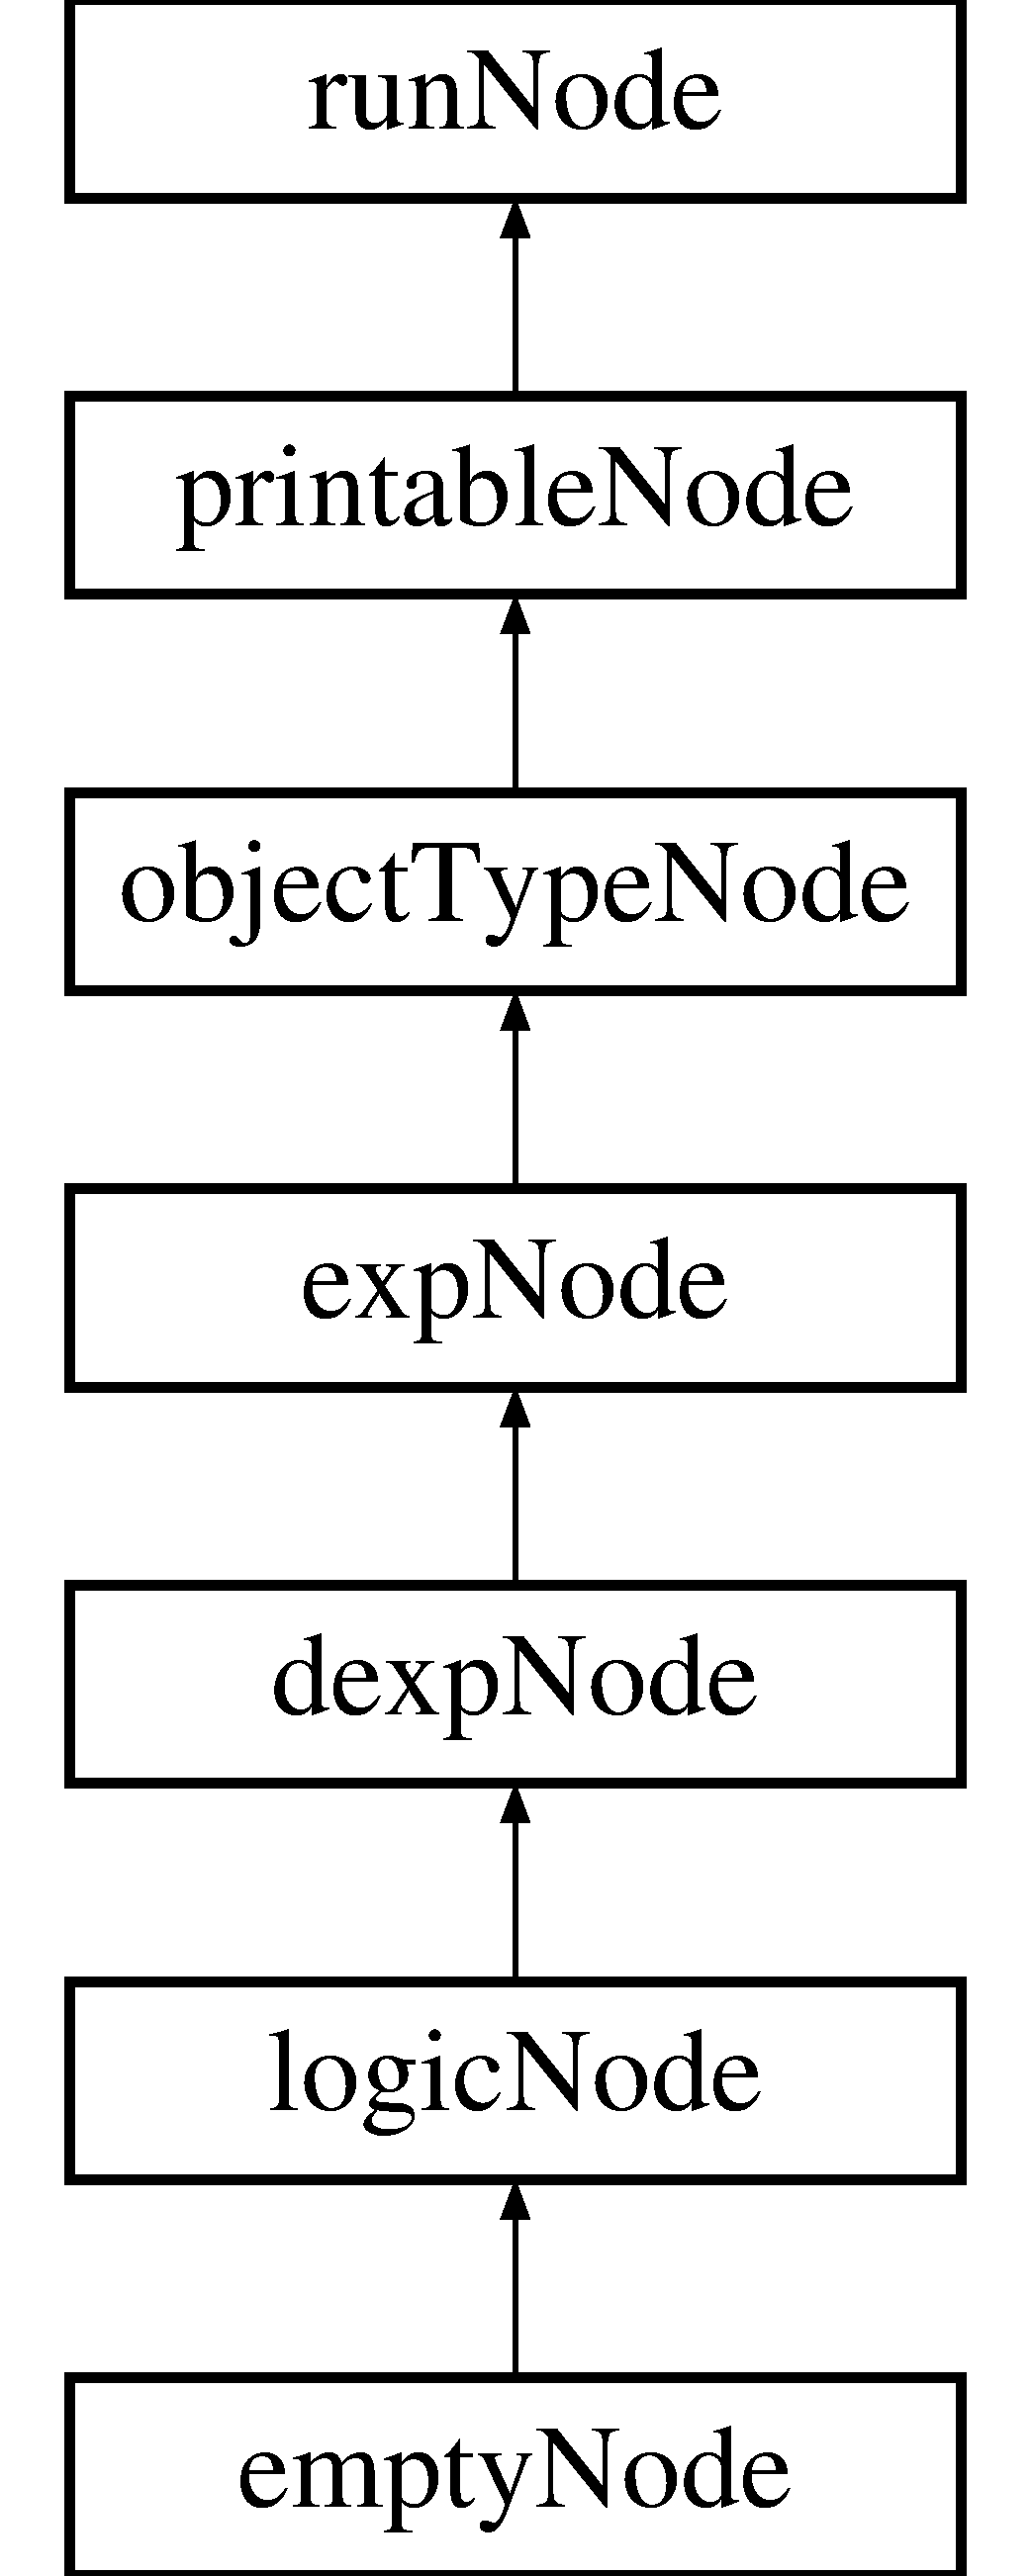
\includegraphics[height=7.000000cm]{classemptyNode}
\end{center}
\end{figure}
\subsection*{Métodos públicos}
\begin{DoxyCompactItemize}
\item 
\hyperlink{classemptyNode_a79b0e2d5d9eb82467c4c9c5d27f6f2e5}{empty\-Node} (\hyperlink{classrunNode}{run\-Node} $\ast$elem)
\item 
void \hyperlink{classemptyNode_ab86f4f2c21cd278bf4d1c07b8d7539a3}{run} ()
\end{DoxyCompactItemize}
\subsection*{Otros miembros heredados}


\subsection{Descripción detallada}
Node operador elemento vacío. 

Este nodo determina si un elemento es vacío. Trabaja sobre diversos tipos de datos.

Si el elemento es booleano toma el valor de la negación, si es númerico toma true si el elemento es 0 y false en caso contrario. Para una cadena de texto toma true si la cadena es la cadena vacía, false en otro caso. Si se trata de una array toma el valor verdadero si este está vacio. 

\subsection{Documentación del constructor y destructor}
\hypertarget{classemptyNode_a79b0e2d5d9eb82467c4c9c5d27f6f2e5}{\index{empty\-Node@{empty\-Node}!empty\-Node@{empty\-Node}}
\index{empty\-Node@{empty\-Node}!emptyNode@{empty\-Node}}
\subsubsection[{empty\-Node}]{\setlength{\rightskip}{0pt plus 5cm}empty\-Node\-::empty\-Node (
\begin{DoxyParamCaption}
\item[{{\bf run\-Node} $\ast$}]{elem}
\end{DoxyParamCaption}
)}}\label{classemptyNode_a79b0e2d5d9eb82467c4c9c5d27f6f2e5}
Constructor de la clase. Asocia el nodo operador a un nodo. 
\begin{DoxyParams}{Parámetros}
{\em elem} & Nodo operando. \\
\hline
\end{DoxyParams}


\subsection{Documentación de las funciones miembro}
\hypertarget{classemptyNode_ab86f4f2c21cd278bf4d1c07b8d7539a3}{\index{empty\-Node@{empty\-Node}!run@{run}}
\index{run@{run}!emptyNode@{empty\-Node}}
\subsubsection[{run}]{\setlength{\rightskip}{0pt plus 5cm}void empty\-Node\-::run (
\begin{DoxyParamCaption}
{}
\end{DoxyParamCaption}
)\hspace{0.3cm}{\ttfamily [virtual]}}}\label{classemptyNode_ab86f4f2c21cd278bf4d1c07b8d7539a3}
Método que ejecuta el nodo. Procede a la ejecución del nodo asociado. y toma como valor un booleano que indica si este representa un elemento vacio. 

Implementa \hyperlink{classrunNode_a83c10df8148829b08e04153c93d69eec}{run\-Node}.



La documentación para esta clase fue generada a partir de los siguientes ficheros\-:\begin{DoxyCompactItemize}
\item 
trunk/src/run/operators/\hyperlink{logicOpNode_8h}{logic\-Op\-Node.\-h}\item 
trunk/src/run/operators/logic\-Op\-Node.\-cpp\end{DoxyCompactItemize}

\hypertarget{classeqNode}{\section{Referencia de la Clase eq\-Node}
\label{classeqNode}\index{eq\-Node@{eq\-Node}}
}


Nodo operador igual que.  




{\ttfamily \#include $<$logic\-Op\-Node.\-h$>$}

Diagrama de herencias de eq\-Node\begin{figure}[H]
\begin{center}
\leavevmode
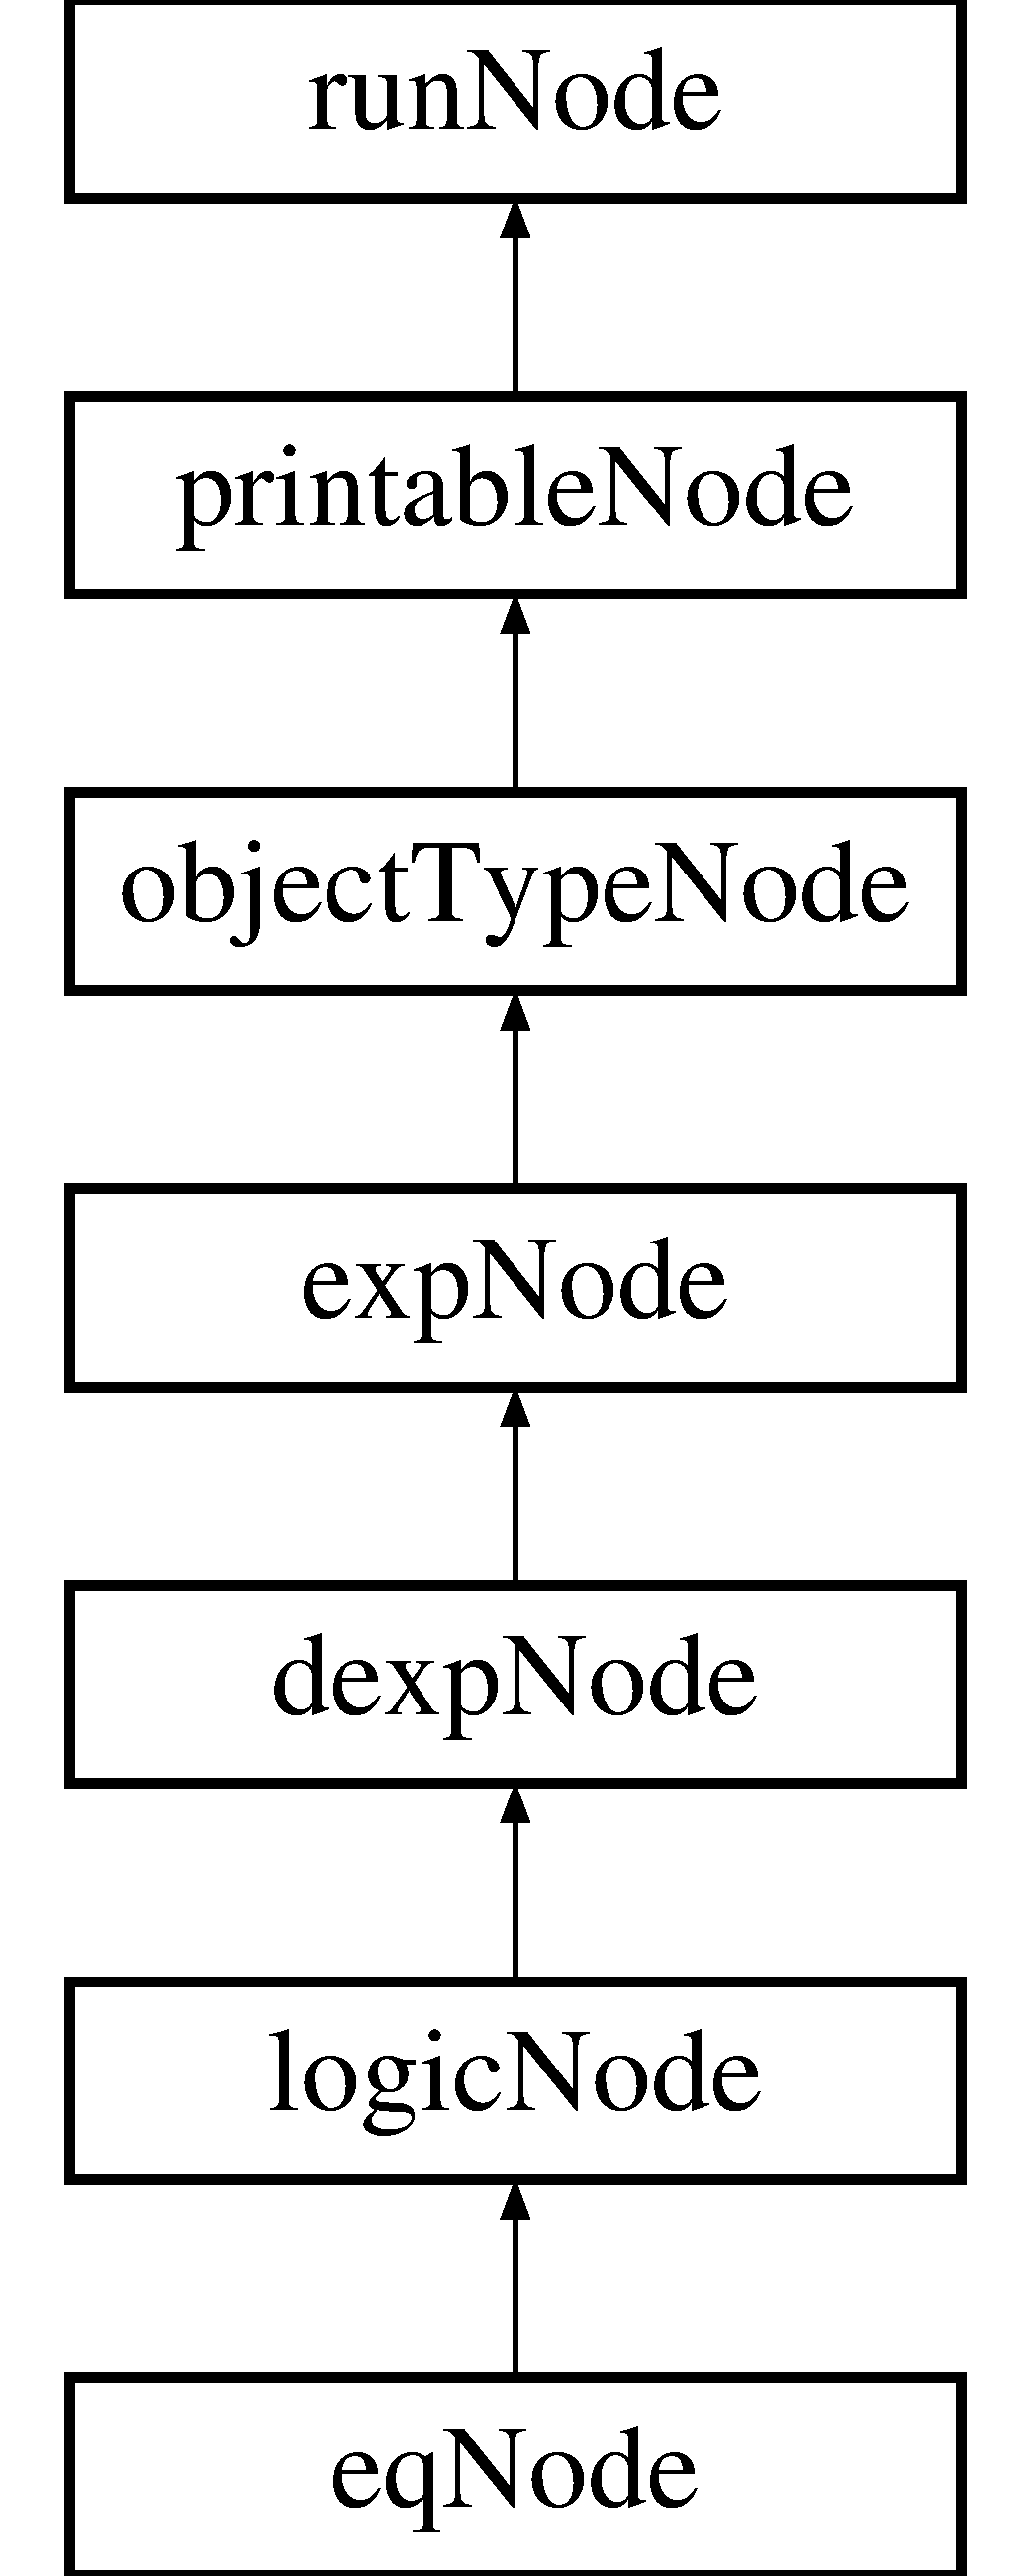
\includegraphics[height=7.000000cm]{classeqNode}
\end{center}
\end{figure}
\subsection*{Métodos públicos}
\begin{DoxyCompactItemize}
\item 
\hyperlink{classeqNode_a8feacf312abba75d46dd634b41719656}{eq\-Node} (\hyperlink{classrunNode}{run\-Node} $\ast$node1, \hyperlink{classrunNode}{run\-Node} $\ast$node2)
\item 
void \hyperlink{classeqNode_a9cbc94f2bc737f97bce1de0acb14c73d}{run} ()
\end{DoxyCompactItemize}
\subsection*{Métodos públicos estáticos}
\begin{DoxyCompactItemize}
\item 
static bool \hyperlink{classeqNode_a7f5ea925683b1d110927db796b3643b1}{do\-\_\-eq} (\hyperlink{classrunNode}{run\-Node} $\ast$op1, \hyperlink{classrunNode}{run\-Node} $\ast$op2)
\end{DoxyCompactItemize}
\subsection*{Otros miembros heredados}


\subsection{Descripción detallada}
Nodo operador igual que. 

Este nodo implementa la operación igual que sobre dos nodos asociados.

Realmente la operación de igualdad se realiza sobre el valor simbólico de los operandos y no sobre el tipo de dato. De esta forma \char`\"{}2\char`\"{} == 2 es verdadero.

El resultado de evaluar la expresión es un valor booleano. 

\subsection{Documentación del constructor y destructor}
\hypertarget{classeqNode_a8feacf312abba75d46dd634b41719656}{\index{eq\-Node@{eq\-Node}!eq\-Node@{eq\-Node}}
\index{eq\-Node@{eq\-Node}!eqNode@{eq\-Node}}
\subsubsection[{eq\-Node}]{\setlength{\rightskip}{0pt plus 5cm}eq\-Node\-::eq\-Node (
\begin{DoxyParamCaption}
\item[{{\bf run\-Node} $\ast$}]{node1, }
\item[{{\bf run\-Node} $\ast$}]{node2}
\end{DoxyParamCaption}
)}}\label{classeqNode_a8feacf312abba75d46dd634b41719656}
Constructor de la clase. Asocia el nodo operador a dos nodos. 
\begin{DoxyParams}{Parámetros}
{\em node1} & Primer nodo operando. \\
\hline
{\em node2} & Sengundo nodo operando. \\
\hline
\end{DoxyParams}


\subsection{Documentación de las funciones miembro}
\hypertarget{classeqNode_a7f5ea925683b1d110927db796b3643b1}{\index{eq\-Node@{eq\-Node}!do\-\_\-eq@{do\-\_\-eq}}
\index{do\-\_\-eq@{do\-\_\-eq}!eqNode@{eq\-Node}}
\subsubsection[{do\-\_\-eq}]{\setlength{\rightskip}{0pt plus 5cm}bool eq\-Node\-::do\-\_\-eq (
\begin{DoxyParamCaption}
\item[{{\bf run\-Node} $\ast$}]{op1, }
\item[{{\bf run\-Node} $\ast$}]{op2}
\end{DoxyParamCaption}
)\hspace{0.3cm}{\ttfamily [static]}}}\label{classeqNode_a7f5ea925683b1d110927db796b3643b1}
Ejecuta la operación igual que sobre dos nodos dados 
\begin{DoxyParams}{Parámetros}
{\em op1} & Primer nodo operando. \\
\hline
{\em op2} & Sengundo nodo operando. \\
\hline
\end{DoxyParams}
\begin{DoxyReturn}{Devuelve}
Valor de la operación 
\end{DoxyReturn}
\hypertarget{classeqNode_a9cbc94f2bc737f97bce1de0acb14c73d}{\index{eq\-Node@{eq\-Node}!run@{run}}
\index{run@{run}!eqNode@{eq\-Node}}
\subsubsection[{run}]{\setlength{\rightskip}{0pt plus 5cm}void eq\-Node\-::run (
\begin{DoxyParamCaption}
{}
\end{DoxyParamCaption}
)\hspace{0.3cm}{\ttfamily [virtual]}}}\label{classeqNode_a9cbc94f2bc737f97bce1de0acb14c73d}
Método que ejecuta el nodo. Procede a la ejecución de los nodos asociados. Luego obtiene el valor lógico del nodo mediante la operación de comparación igual que entre el valor numérico de los dos nodos. 

Implementa \hyperlink{classrunNode_a83c10df8148829b08e04153c93d69eec}{run\-Node}.



La documentación para esta clase fue generada a partir de los siguientes ficheros\-:\begin{DoxyCompactItemize}
\item 
trunk/src/run/operators/\hyperlink{logicOpNode_8h}{logic\-Op\-Node.\-h}\item 
trunk/src/run/operators/logic\-Op\-Node.\-cpp\end{DoxyCompactItemize}

\hypertarget{classevalNode}{\section{Referencia de la Clase eval\-Node}
\label{classevalNode}\index{eval\-Node@{eval\-Node}}
}


Node operador evaluación.  




{\ttfamily \#include $<$process\-Op\-Node.\-h$>$}

Diagrama de herencias de eval\-Node\begin{figure}[H]
\begin{center}
\leavevmode
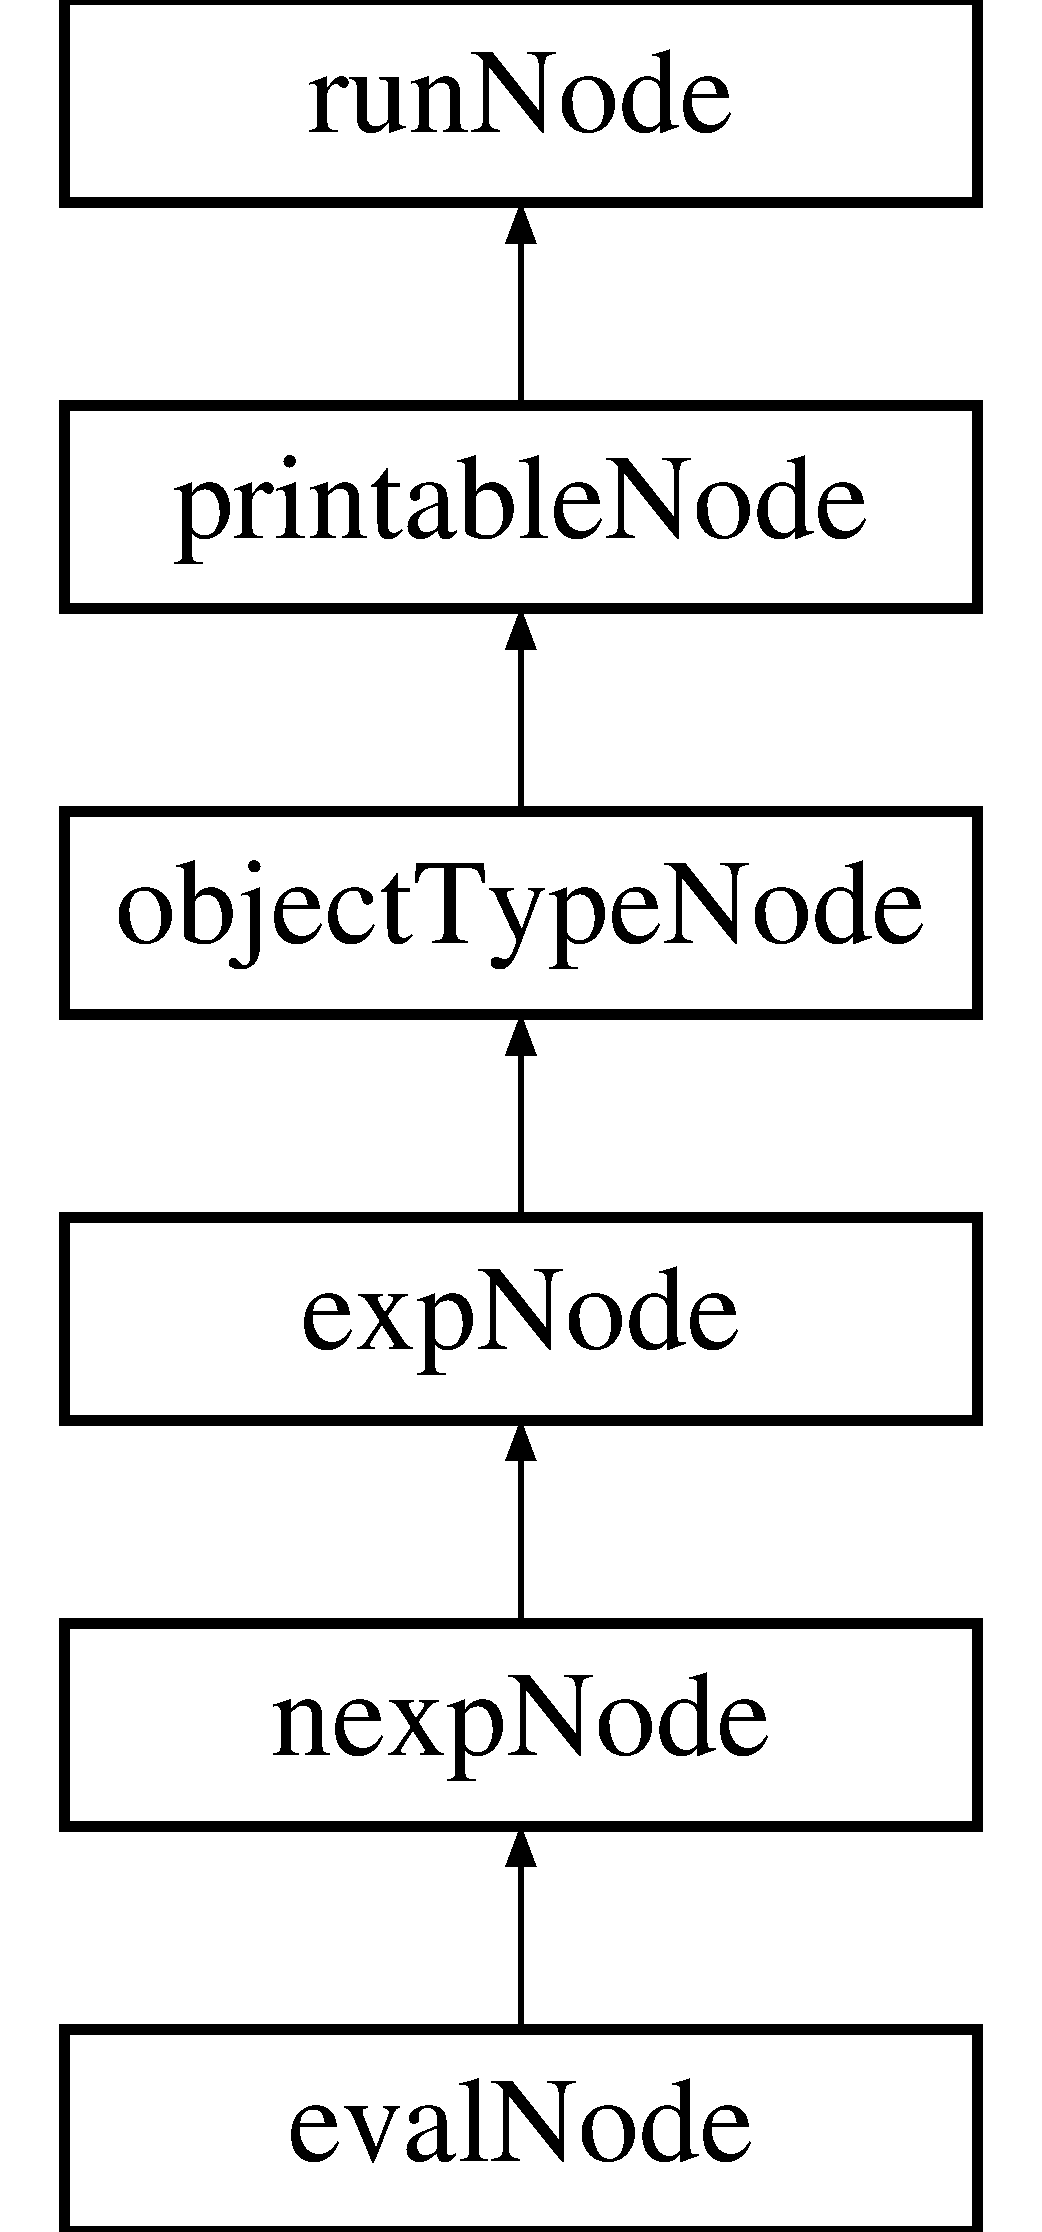
\includegraphics[height=6.000000cm]{classevalNode}
\end{center}
\end{figure}
\subsection*{Métodos públicos}
\begin{DoxyCompactItemize}
\item 
\hyperlink{classevalNode_ade792e8e711f68ccac607e929e75f8b8}{eval\-Node} (\hyperlink{classrunNode}{run\-Node} $\ast$node)
\item 
void \hyperlink{classevalNode_a09885abc979cca1e769cb83e32017909}{run} ()
\end{DoxyCompactItemize}
\subsection*{Otros miembros heredados}


\subsection{Descripción detallada}
Node operador evaluación. 

Este nodo procesa y evalua una cadena como si de codigo fuente se tratase. Como valor toma el resultado devuelto por la primera sentencia return ejecutada al evaluar la cadena. 

\subsection{Documentación del constructor y destructor}
\hypertarget{classevalNode_ade792e8e711f68ccac607e929e75f8b8}{\index{eval\-Node@{eval\-Node}!eval\-Node@{eval\-Node}}
\index{eval\-Node@{eval\-Node}!evalNode@{eval\-Node}}
\subsubsection[{eval\-Node}]{\setlength{\rightskip}{0pt plus 5cm}eval\-Node\-::eval\-Node (
\begin{DoxyParamCaption}
\item[{{\bf run\-Node} $\ast$}]{node}
\end{DoxyParamCaption}
)}}\label{classevalNode_ade792e8e711f68ccac607e929e75f8b8}
Constructor de la clase. 
\begin{DoxyParams}{Parámetros}
{\em node.} & Nodo que representa la cadena que será interpretada \\
\hline
\end{DoxyParams}


\subsection{Documentación de las funciones miembro}
\hypertarget{classevalNode_a09885abc979cca1e769cb83e32017909}{\index{eval\-Node@{eval\-Node}!run@{run}}
\index{run@{run}!evalNode@{eval\-Node}}
\subsubsection[{run}]{\setlength{\rightskip}{0pt plus 5cm}void eval\-Node\-::run (
\begin{DoxyParamCaption}
{}
\end{DoxyParamCaption}
)\hspace{0.3cm}{\ttfamily [virtual]}}}\label{classevalNode_a09885abc979cca1e769cb83e32017909}
Metodo de ejecución. Procede a la ejecución del nodo asociado que representa una cadena de codigo fuente. Toma como valor el resultado devuelto por la primera sentencia return evaluada, si no se ejecuta una sentencia return al procesar la cadena se tomará como valor el nodo nulo. 

Implementa \hyperlink{classrunNode_a83c10df8148829b08e04153c93d69eec}{run\-Node}.



La documentación para esta clase fue generada a partir de los siguientes ficheros\-:\begin{DoxyCompactItemize}
\item 
trunk/src/run/operators/\hyperlink{processOpNode_8h}{process\-Op\-Node.\-h}\item 
trunk/src/run/operators/process\-Op\-Node.\-cpp\end{DoxyCompactItemize}

\hypertarget{classexecNode}{\section{Referencia de la Clase exec\-Node}
\label{classexecNode}\index{exec\-Node@{exec\-Node}}
}


Node operador ejecución de comando.  




{\ttfamily \#include $<$process\-Op\-Node.\-h$>$}

Diagrama de herencias de exec\-Node\begin{figure}[H]
\begin{center}
\leavevmode
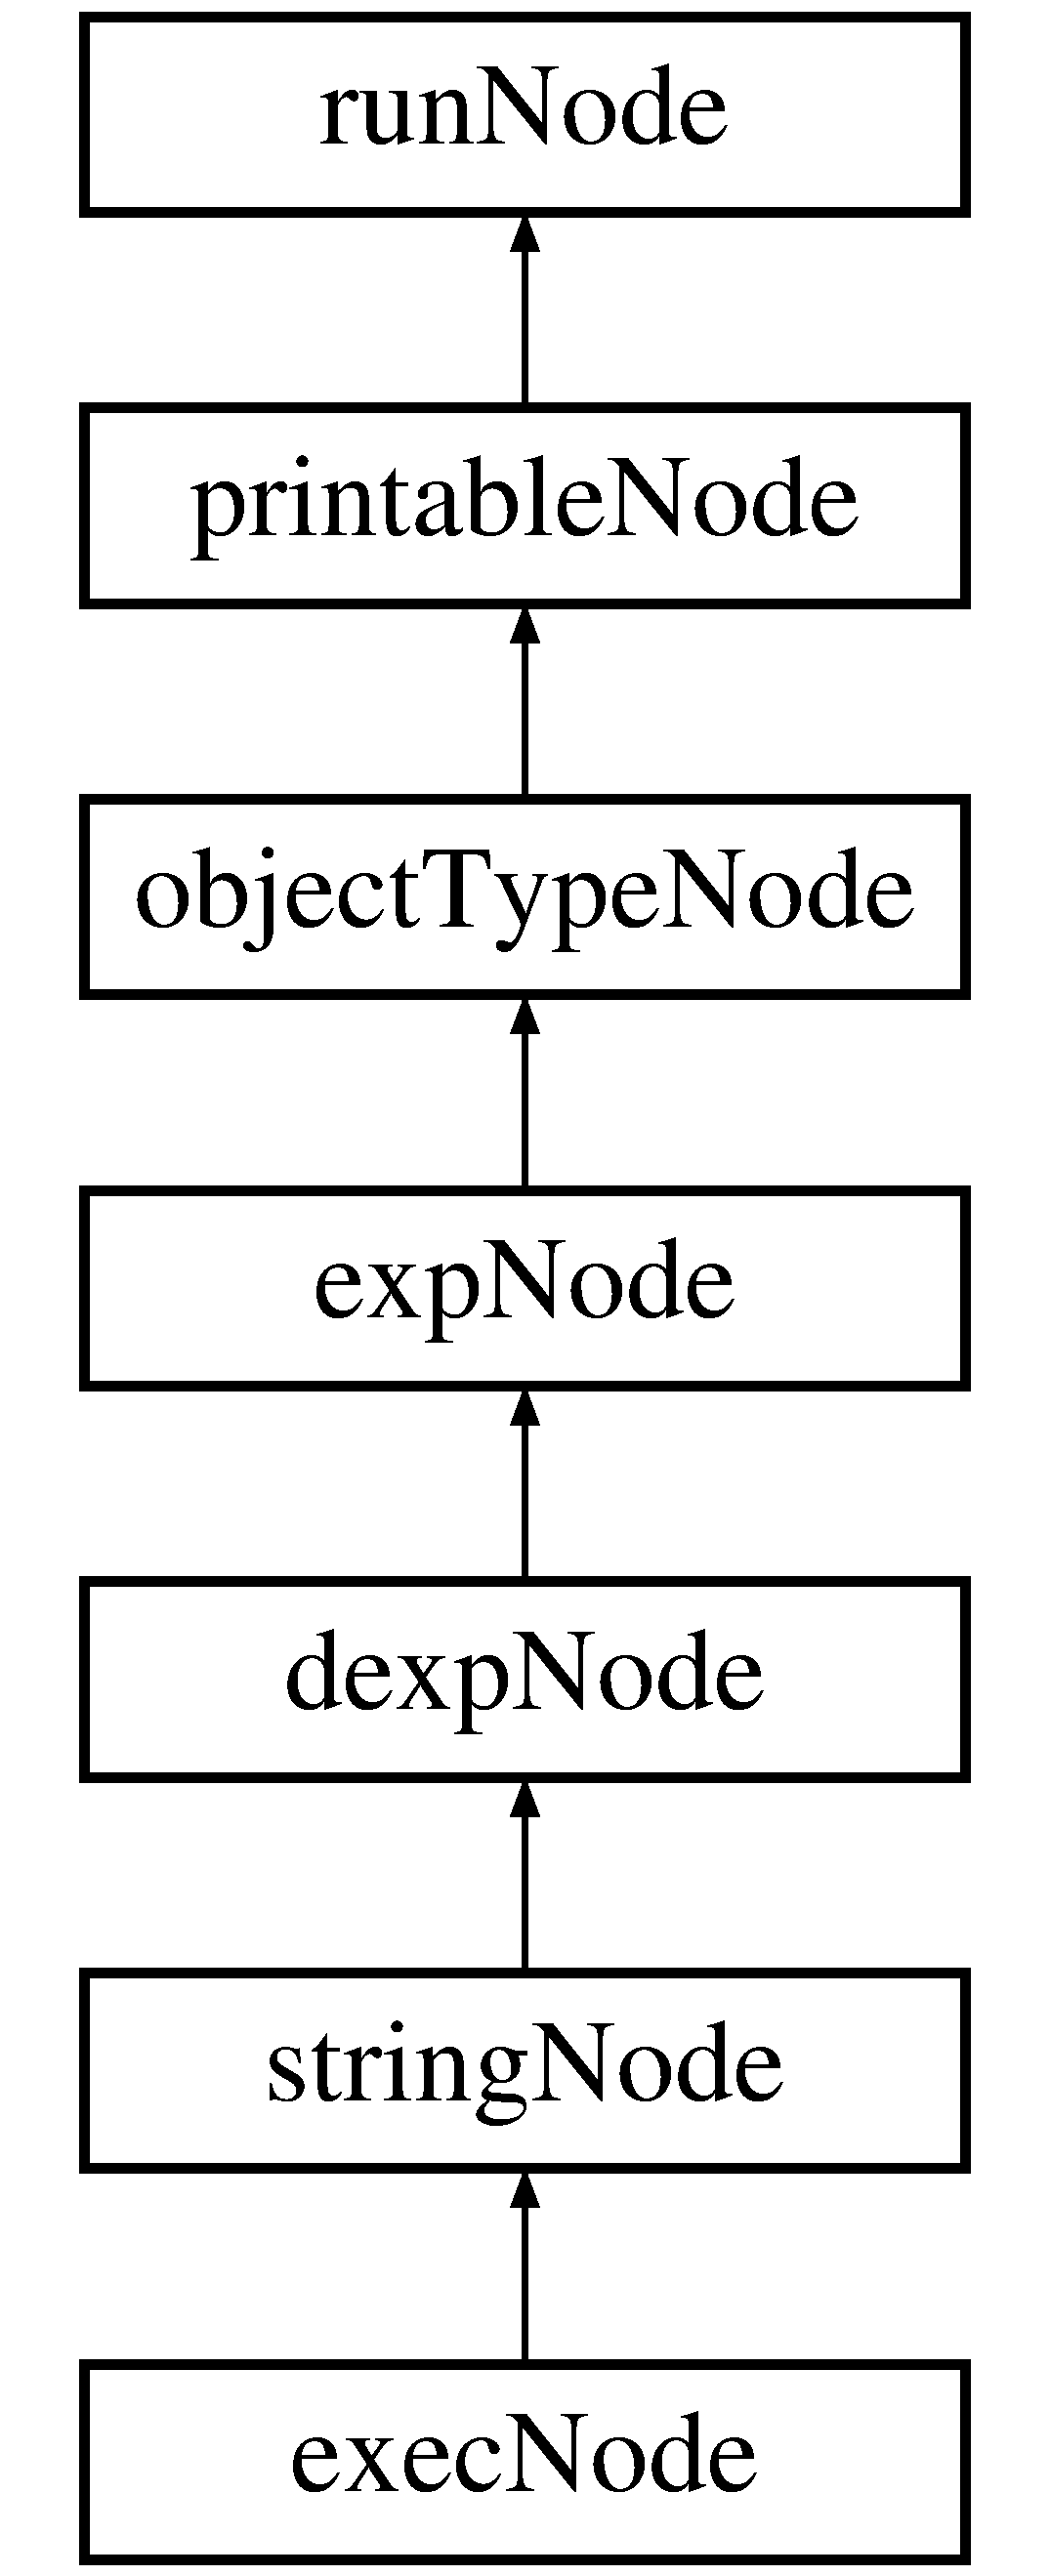
\includegraphics[height=7.000000cm]{classexecNode}
\end{center}
\end{figure}
\subsection*{Métodos públicos}
\begin{DoxyCompactItemize}
\item 
\hyperlink{classexecNode_a58d08383a1a96a62d012c1288069a619}{exec\-Node} (\hyperlink{classrunNode}{run\-Node} $\ast$node)
\item 
void \hyperlink{classexecNode_a0eec036e65db650fa5a58e92dfbfb967}{run} ()
\end{DoxyCompactItemize}
\subsection*{Otros miembros heredados}


\subsection{Descripción detallada}
Node operador ejecución de comando. 

Este nodo se encarga de ejecutar un comando en el sistema tomando como valor la salida del mismo. 

\subsection{Documentación del constructor y destructor}
\hypertarget{classexecNode_a58d08383a1a96a62d012c1288069a619}{\index{exec\-Node@{exec\-Node}!exec\-Node@{exec\-Node}}
\index{exec\-Node@{exec\-Node}!execNode@{exec\-Node}}
\subsubsection[{exec\-Node}]{\setlength{\rightskip}{0pt plus 5cm}exec\-Node\-::exec\-Node (
\begin{DoxyParamCaption}
\item[{{\bf run\-Node} $\ast$}]{node}
\end{DoxyParamCaption}
)}}\label{classexecNode_a58d08383a1a96a62d012c1288069a619}
Constructor de la clase. 
\begin{DoxyParams}{Parámetros}
{\em node.} & Nodo comando \\
\hline
\end{DoxyParams}


\subsection{Documentación de las funciones miembro}
\hypertarget{classexecNode_a0eec036e65db650fa5a58e92dfbfb967}{\index{exec\-Node@{exec\-Node}!run@{run}}
\index{run@{run}!execNode@{exec\-Node}}
\subsubsection[{run}]{\setlength{\rightskip}{0pt plus 5cm}void exec\-Node\-::run (
\begin{DoxyParamCaption}
{}
\end{DoxyParamCaption}
)\hspace{0.3cm}{\ttfamily [virtual]}}}\label{classexecNode_a0eec036e65db650fa5a58e92dfbfb967}
Metodo de ejecución. Procede a la ejecución del nodo que hace de comando. Toma como valor el resultado de la ejecución de este en el sistema 

Implementa \hyperlink{classrunNode_a83c10df8148829b08e04153c93d69eec}{run\-Node}.



La documentación para esta clase fue generada a partir de los siguientes ficheros\-:\begin{DoxyCompactItemize}
\item 
trunk/src/run/operators/\hyperlink{processOpNode_8h}{process\-Op\-Node.\-h}\item 
trunk/src/run/operators/process\-Op\-Node.\-cpp\end{DoxyCompactItemize}

\hypertarget{classexitNode}{\section{Referencia de la Clase exit\-Node}
\label{classexitNode}\index{exit\-Node@{exit\-Node}}
}


Nodo sentencia de finalización.  




{\ttfamily \#include $<$stmt\-Node.\-h$>$}

Diagrama de herencias de exit\-Node\begin{figure}[H]
\begin{center}
\leavevmode
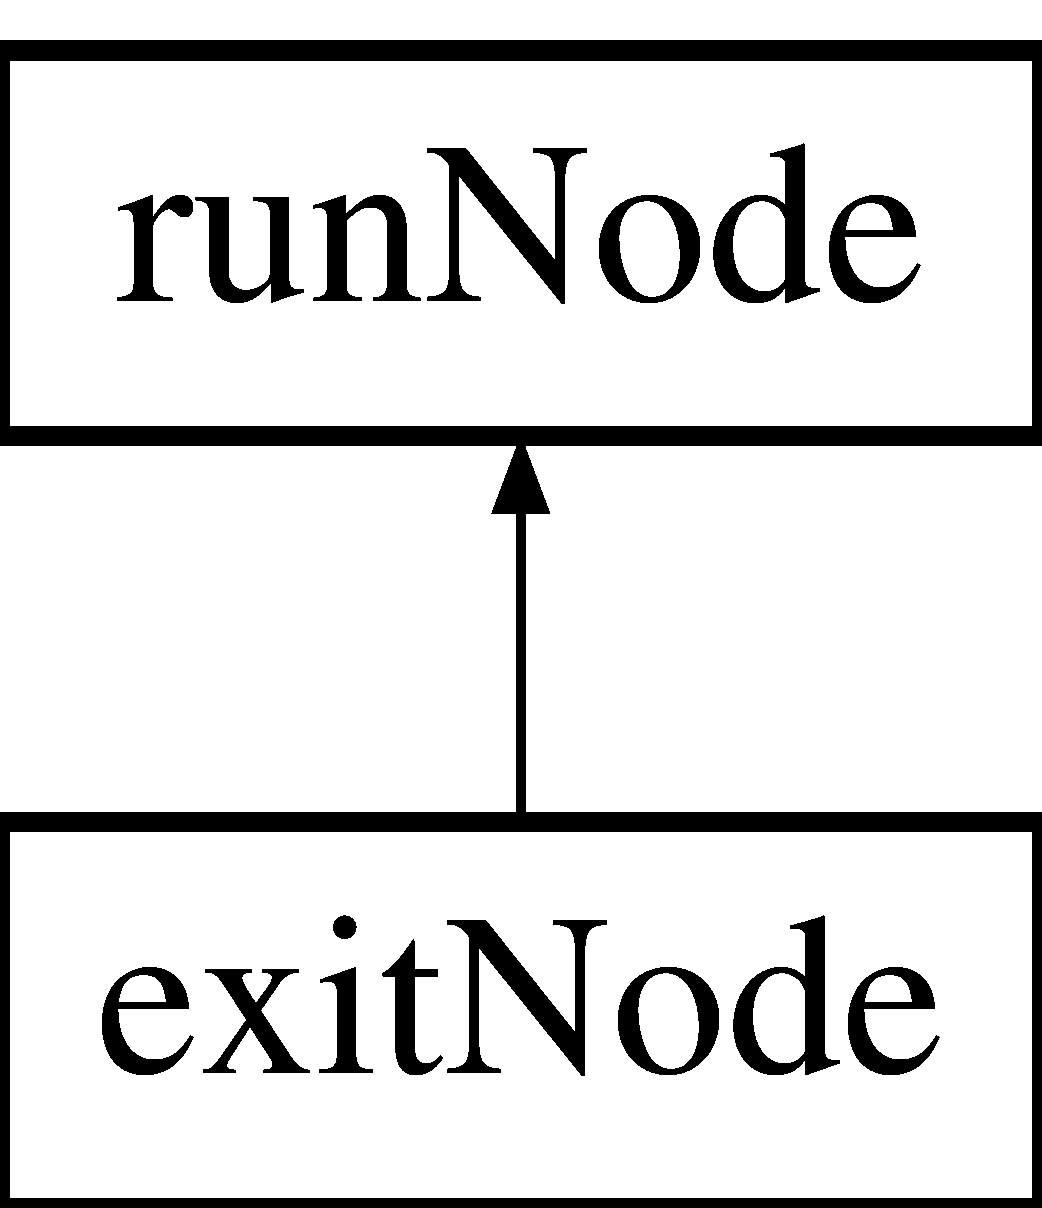
\includegraphics[height=2.000000cm]{classexitNode}
\end{center}
\end{figure}
\subsection*{Métodos públicos}
\begin{DoxyCompactItemize}
\item 
void \hyperlink{classexitNode_afdb1e6ff54c0d3c4a5ef2ec1d9f40326}{run} ()
\end{DoxyCompactItemize}
\subsection*{Otros miembros heredados}


\subsection{Descripción detallada}
Nodo sentencia de finalización. 

Nodo que finaliza la ejecución del programa 

\subsection{Documentación de las funciones miembro}
\hypertarget{classexitNode_afdb1e6ff54c0d3c4a5ef2ec1d9f40326}{\index{exit\-Node@{exit\-Node}!run@{run}}
\index{run@{run}!exitNode@{exit\-Node}}
\subsubsection[{run}]{\setlength{\rightskip}{0pt plus 5cm}void exit\-Node\-::run (
\begin{DoxyParamCaption}
{}
\end{DoxyParamCaption}
)\hspace{0.3cm}{\ttfamily [virtual]}}}\label{classexitNode_afdb1e6ff54c0d3c4a5ef2ec1d9f40326}
Método que ejecuta el nodo. Finaliza la ejecución del programa con un estado de 0 

Implementa \hyperlink{classrunNode_a83c10df8148829b08e04153c93d69eec}{run\-Node}.



La documentación para esta clase fue generada a partir de los siguientes ficheros\-:\begin{DoxyCompactItemize}
\item 
trunk/src/run/stmts/\hyperlink{stmtNode_8h}{stmt\-Node.\-h}\item 
trunk/src/run/stmts/stmt\-Node.\-cpp\end{DoxyCompactItemize}

\hypertarget{classexitProcessNode}{\section{Referencia de la Clase exit\-Process\-Node}
\label{classexitProcessNode}\index{exit\-Process\-Node@{exit\-Process\-Node}}
}


Nodo función finalización de proceso.  




{\ttfamily \#include $<$process\-Op\-Node.\-h$>$}

Diagrama de herencias de exit\-Process\-Node\begin{figure}[H]
\begin{center}
\leavevmode
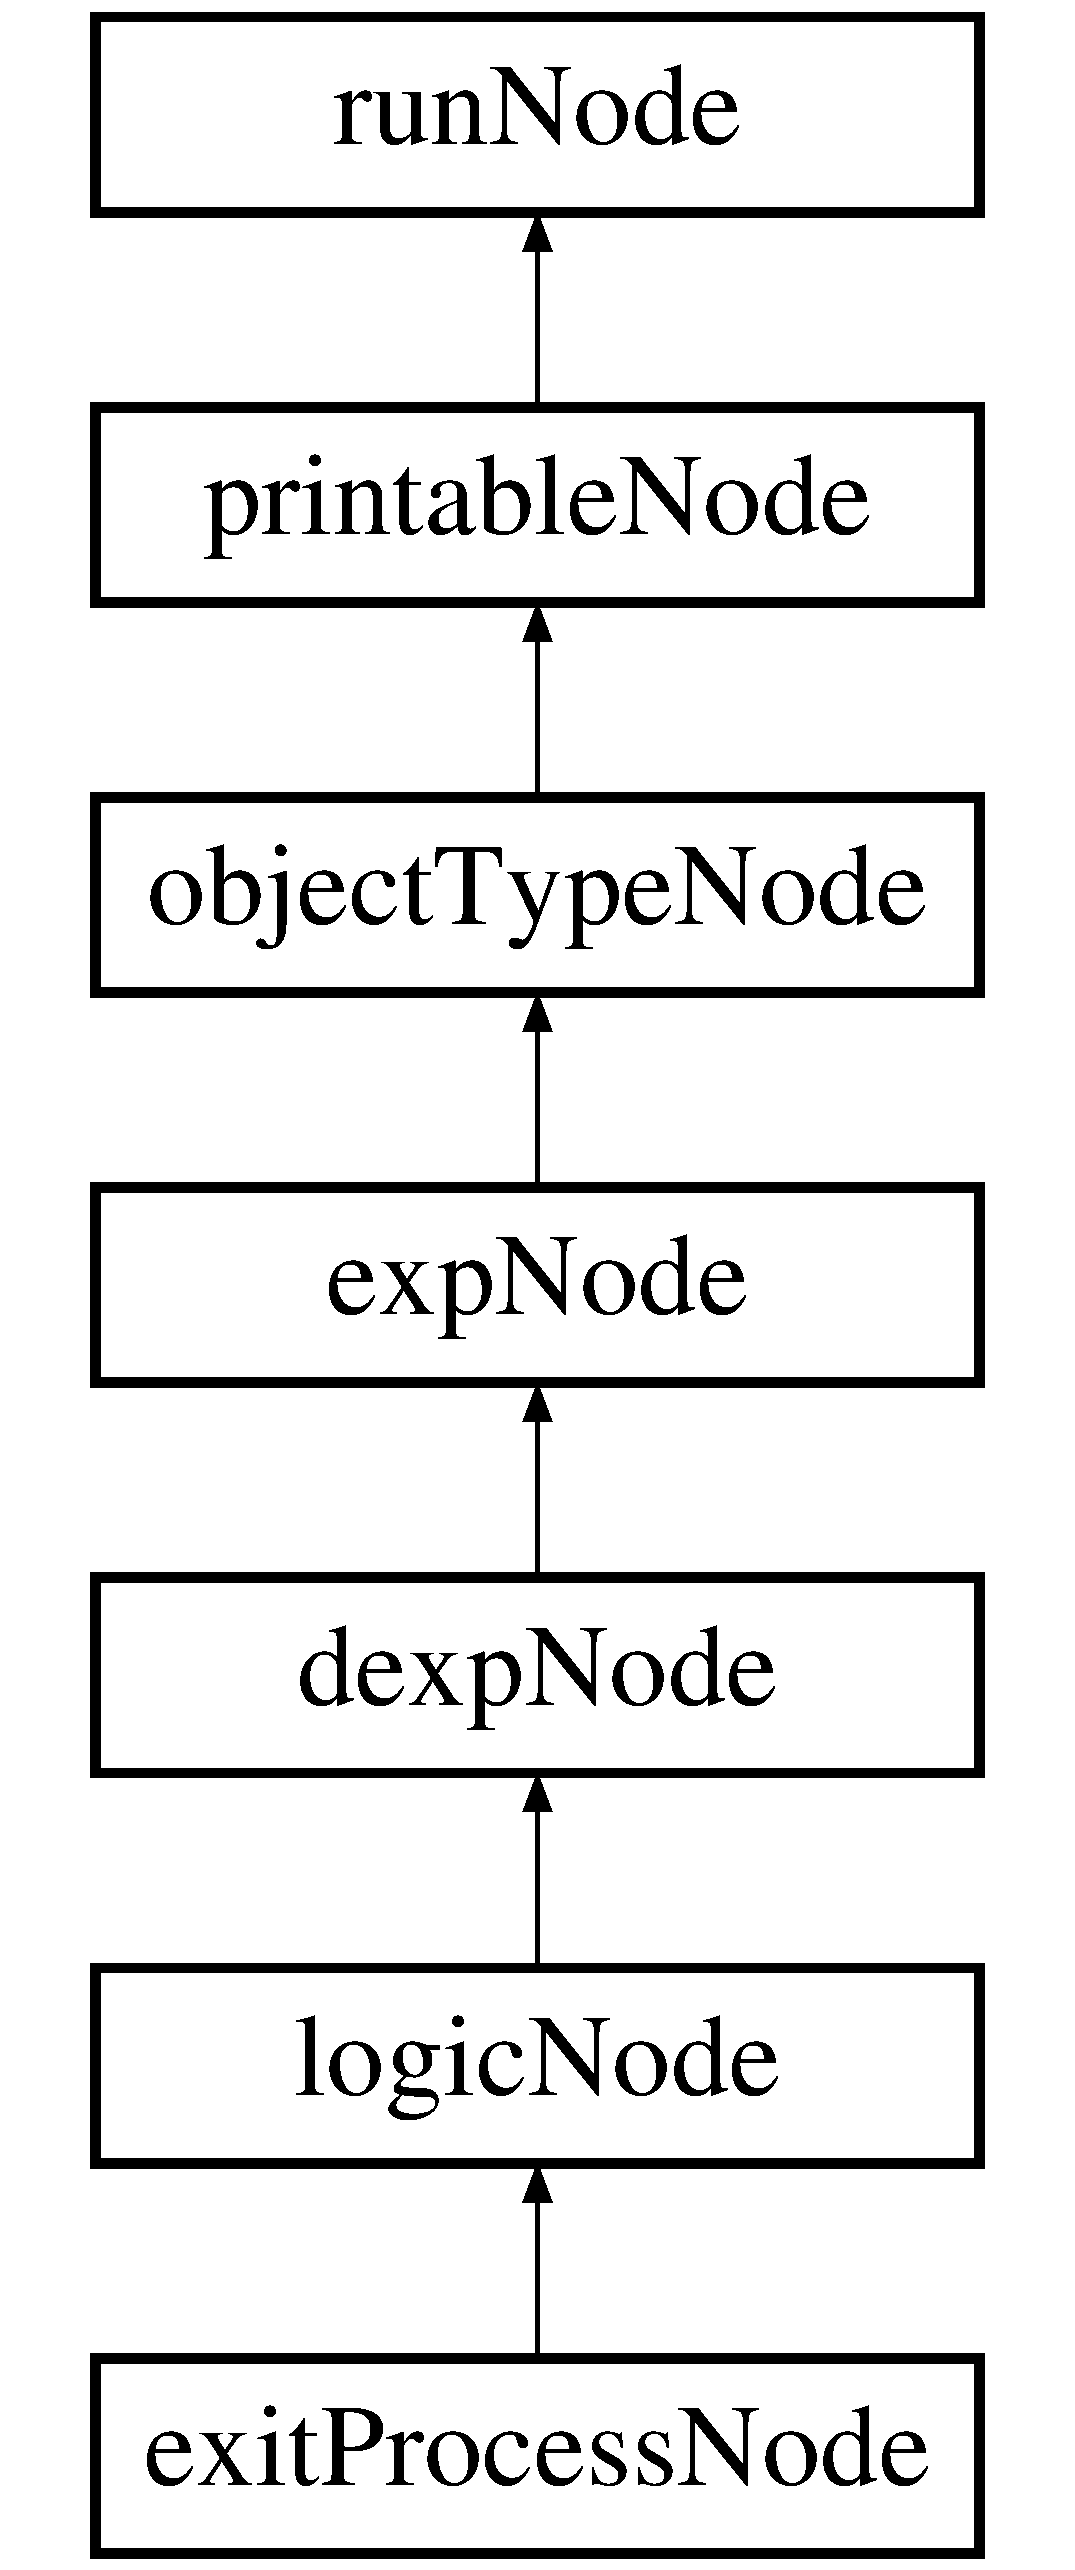
\includegraphics[height=7.000000cm]{classexitProcessNode}
\end{center}
\end{figure}
\subsection*{Métodos públicos}
\begin{DoxyCompactItemize}
\item 
\hyperlink{classexitProcessNode_afc99e1ac323ccd4dda5173cf2c2d987b}{exit\-Process\-Node} ()
\item 
void \hyperlink{classexitProcessNode_ab68ac4e38c752216e5cc5960994dc111}{run} ()
\end{DoxyCompactItemize}
\subsection*{Otros miembros heredados}


\subsection{Descripción detallada}
Nodo función finalización de proceso. 

Finaliza la ejecución del proceso actual 

\subsection{Documentación del constructor y destructor}
\hypertarget{classexitProcessNode_afc99e1ac323ccd4dda5173cf2c2d987b}{\index{exit\-Process\-Node@{exit\-Process\-Node}!exit\-Process\-Node@{exit\-Process\-Node}}
\index{exit\-Process\-Node@{exit\-Process\-Node}!exitProcessNode@{exit\-Process\-Node}}
\subsubsection[{exit\-Process\-Node}]{\setlength{\rightskip}{0pt plus 5cm}exit\-Process\-Node\-::exit\-Process\-Node (
\begin{DoxyParamCaption}
{}
\end{DoxyParamCaption}
)}}\label{classexitProcessNode_afc99e1ac323ccd4dda5173cf2c2d987b}
Constructor de la clase. 

\subsection{Documentación de las funciones miembro}
\hypertarget{classexitProcessNode_ab68ac4e38c752216e5cc5960994dc111}{\index{exit\-Process\-Node@{exit\-Process\-Node}!run@{run}}
\index{run@{run}!exitProcessNode@{exit\-Process\-Node}}
\subsubsection[{run}]{\setlength{\rightskip}{0pt plus 5cm}void exit\-Process\-Node\-::run (
\begin{DoxyParamCaption}
{}
\end{DoxyParamCaption}
)\hspace{0.3cm}{\ttfamily [virtual]}}}\label{classexitProcessNode_ab68ac4e38c752216e5cc5960994dc111}
Metodo de ejecución. Finaliza la ejecución del proceso actua. Como valor se toma un valor booleano que indica si el proceso se llevó a cabo de forma correcta. 

Implementa \hyperlink{classrunNode_a83c10df8148829b08e04153c93d69eec}{run\-Node}.



La documentación para esta clase fue generada a partir de los siguientes ficheros\-:\begin{DoxyCompactItemize}
\item 
trunk/src/run/operators/\hyperlink{processOpNode_8h}{process\-Op\-Node.\-h}\item 
trunk/src/run/operators/process\-Op\-Node.\-cpp\end{DoxyCompactItemize}

\hypertarget{classexplodeNode}{\section{Referencia de la Clase explode\-Node}
\label{classexplodeNode}\index{explode\-Node@{explode\-Node}}
}


Nodo operador explode.  




{\ttfamily \#include $<$str\-Op\-Node.\-h$>$}

Diagrama de herencias de explode\-Node\begin{figure}[H]
\begin{center}
\leavevmode
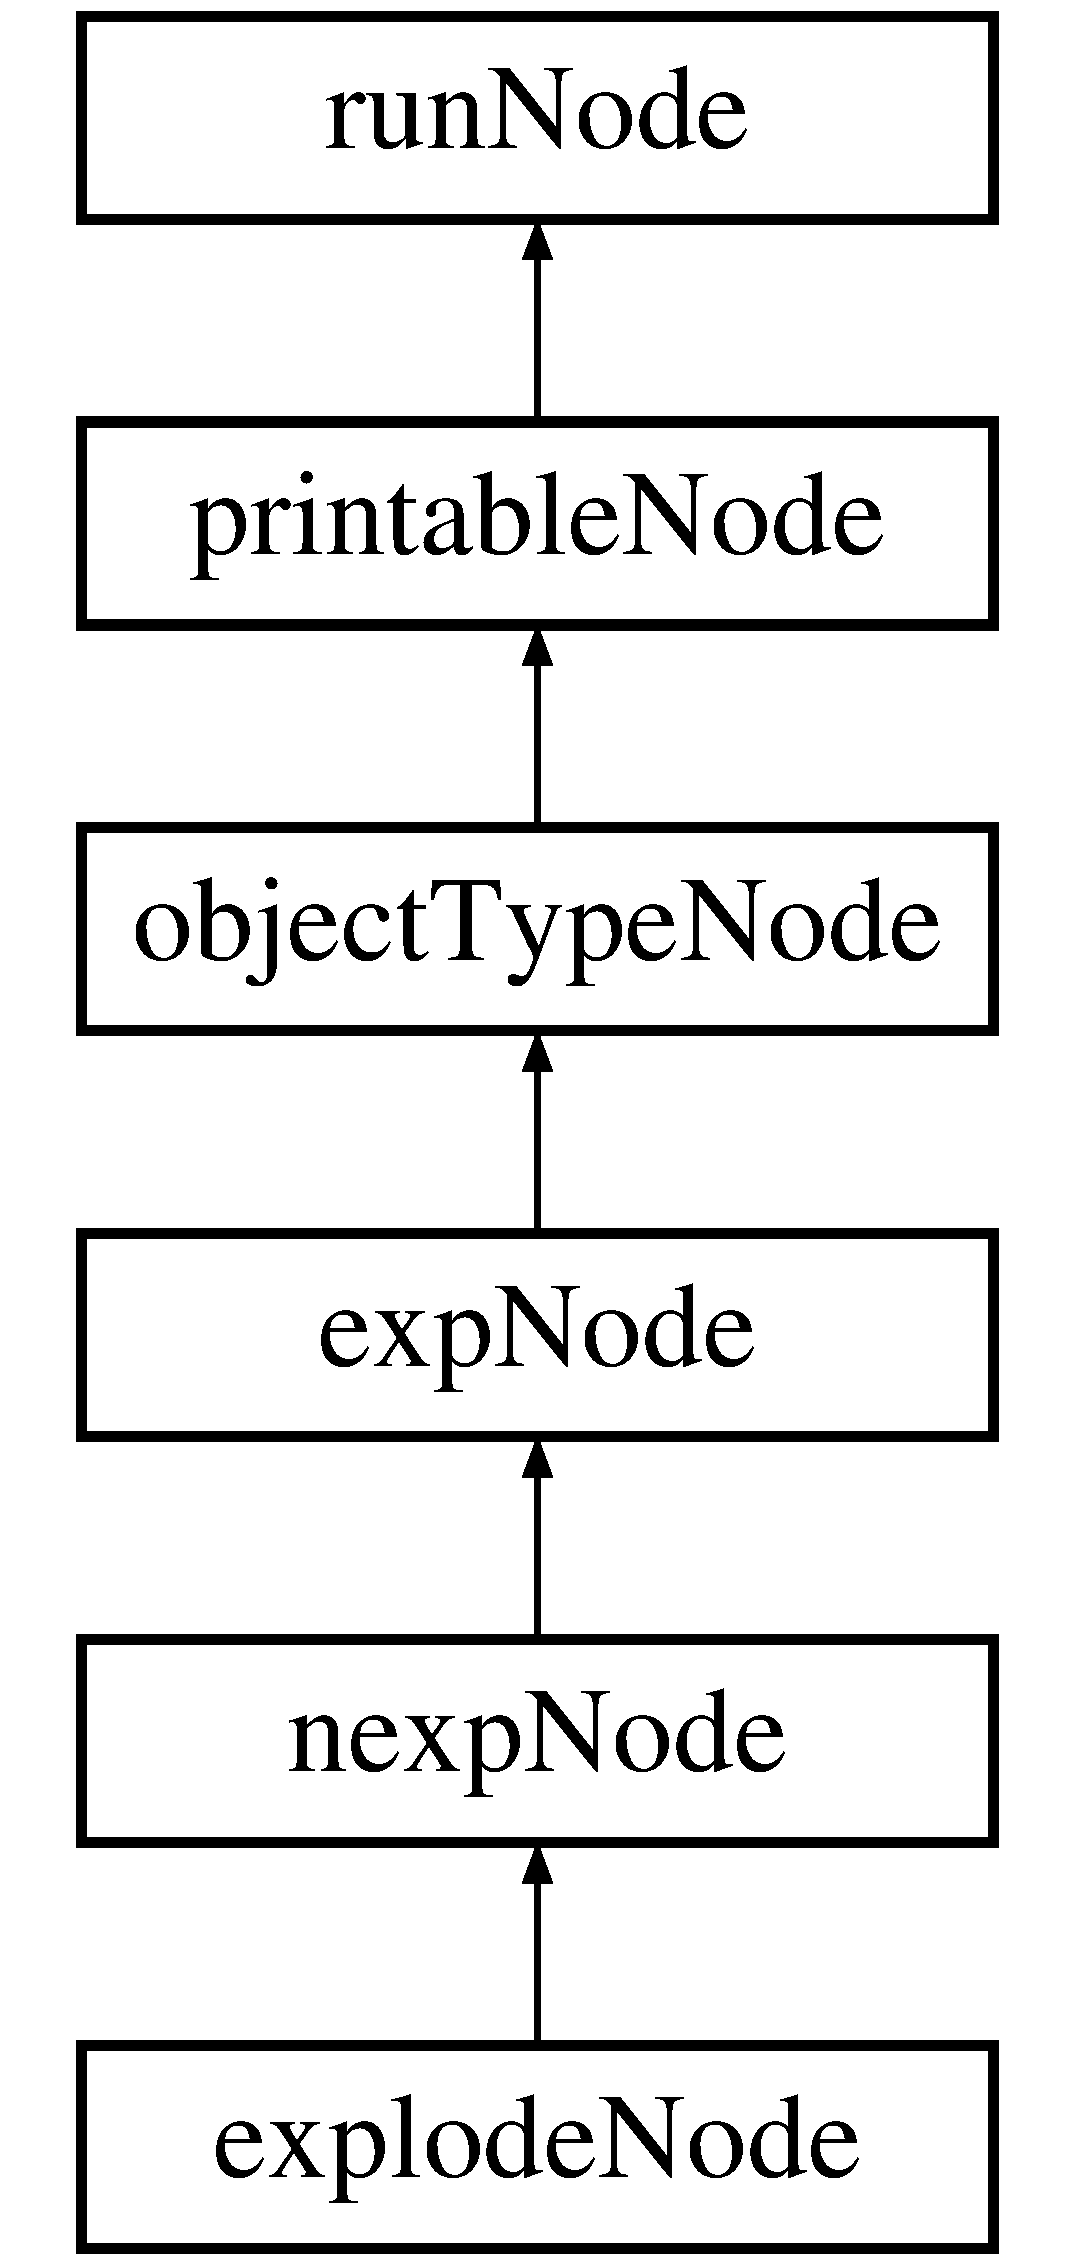
\includegraphics[height=6.000000cm]{classexplodeNode}
\end{center}
\end{figure}
\subsection*{Métodos públicos}
\begin{DoxyCompactItemize}
\item 
\hyperlink{classexplodeNode_a90c920b30840535e2ad7c27913e91f7c}{explode\-Node} (\hyperlink{classrunNode}{run\-Node} $\ast$substr, \hyperlink{classrunNode}{run\-Node} $\ast$str)
\item 
void \hyperlink{classexplodeNode_a1bb7df027458cb1e63d5b0898540b114}{run} ()
\end{DoxyCompactItemize}
\subsection*{Métodos públicos estáticos}
\begin{DoxyCompactItemize}
\item 
static \hyperlink{classrunNode}{run\-Node} $\ast$ \hyperlink{classexplodeNode_aea0516f602785514e0a709b4f0867774}{as\-Method} ()
\end{DoxyCompactItemize}


\subsection{Descripción detallada}
Nodo operador explode. 

Este operador permite dividir en partes una cadena de texto a partir de una subcadena denominada separador

El nodo toma como valor un array que contedrá cada una de las subscadenas en que queda dividida la cadena principal por el separador. 

\subsection{Documentación del constructor y destructor}
\hypertarget{classexplodeNode_a90c920b30840535e2ad7c27913e91f7c}{\index{explode\-Node@{explode\-Node}!explode\-Node@{explode\-Node}}
\index{explode\-Node@{explode\-Node}!explodeNode@{explode\-Node}}
\subsubsection[{explode\-Node}]{\setlength{\rightskip}{0pt plus 5cm}explode\-Node\-::explode\-Node (
\begin{DoxyParamCaption}
\item[{{\bf run\-Node} $\ast$}]{substr, }
\item[{{\bf run\-Node} $\ast$}]{str}
\end{DoxyParamCaption}
)}}\label{classexplodeNode_a90c920b30840535e2ad7c27913e91f7c}
Constructor principal a partir de la subcadena separador y la cadena a dividir 
\begin{DoxyParams}{Parámetros}
{\em substr} & Nodo subcadena que se usará como separador \\
\hline
{\em str} & Nodo cadena al que se realizará la operación \\
\hline
\end{DoxyParams}


\subsection{Documentación de las funciones miembro}
\hypertarget{classexplodeNode_aea0516f602785514e0a709b4f0867774}{\index{explode\-Node@{explode\-Node}!as\-Method@{as\-Method}}
\index{as\-Method@{as\-Method}!explodeNode@{explode\-Node}}
\subsubsection[{as\-Method}]{\setlength{\rightskip}{0pt plus 5cm}{\bf run\-Node} $\ast$ explode\-Node\-::as\-Method (
\begin{DoxyParamCaption}
{}
\end{DoxyParamCaption}
)\hspace{0.3cm}{\ttfamily [static]}}}\label{classexplodeNode_aea0516f602785514e0a709b4f0867774}
Devuelve un nodo explode como cuerpo de un nodo función, siendo un nodo this la cadena. \begin{DoxyReturn}{Devuelve}
Método explode. 
\end{DoxyReturn}
\hypertarget{classexplodeNode_a1bb7df027458cb1e63d5b0898540b114}{\index{explode\-Node@{explode\-Node}!run@{run}}
\index{run@{run}!explodeNode@{explode\-Node}}
\subsubsection[{run}]{\setlength{\rightskip}{0pt plus 5cm}void explode\-Node\-::run (
\begin{DoxyParamCaption}
{}
\end{DoxyParamCaption}
)\hspace{0.3cm}{\ttfamily [virtual]}}}\label{classexplodeNode_a1bb7df027458cb1e63d5b0898540b114}
La ejecución del nodo consite en dividir la cadena principal haciendo uso del separador. Cada una de las subcadenas en la que queda dividida la cadena principal se guardan en un array por orden posicional.

El nodo tomará como valor el array resultante. 

Implementa \hyperlink{classrunNode_a83c10df8148829b08e04153c93d69eec}{run\-Node}.



La documentación para esta clase fue generada a partir de los siguientes ficheros\-:\begin{DoxyCompactItemize}
\item 
trunk/src/run/operators/\hyperlink{strOpNode_8h}{str\-Op\-Node.\-h}\item 
trunk/src/run/operators/str\-Op\-Node.\-cpp\end{DoxyCompactItemize}

\hypertarget{classexpNode}{\section{Referencia de la Clase exp\-Node}
\label{classexpNode}\index{exp\-Node@{exp\-Node}}
}


Nodo de expresión.  




{\ttfamily \#include $<$exp\-Node.\-h$>$}

Diagrama de herencias de exp\-Node\begin{figure}[H]
\begin{center}
\leavevmode
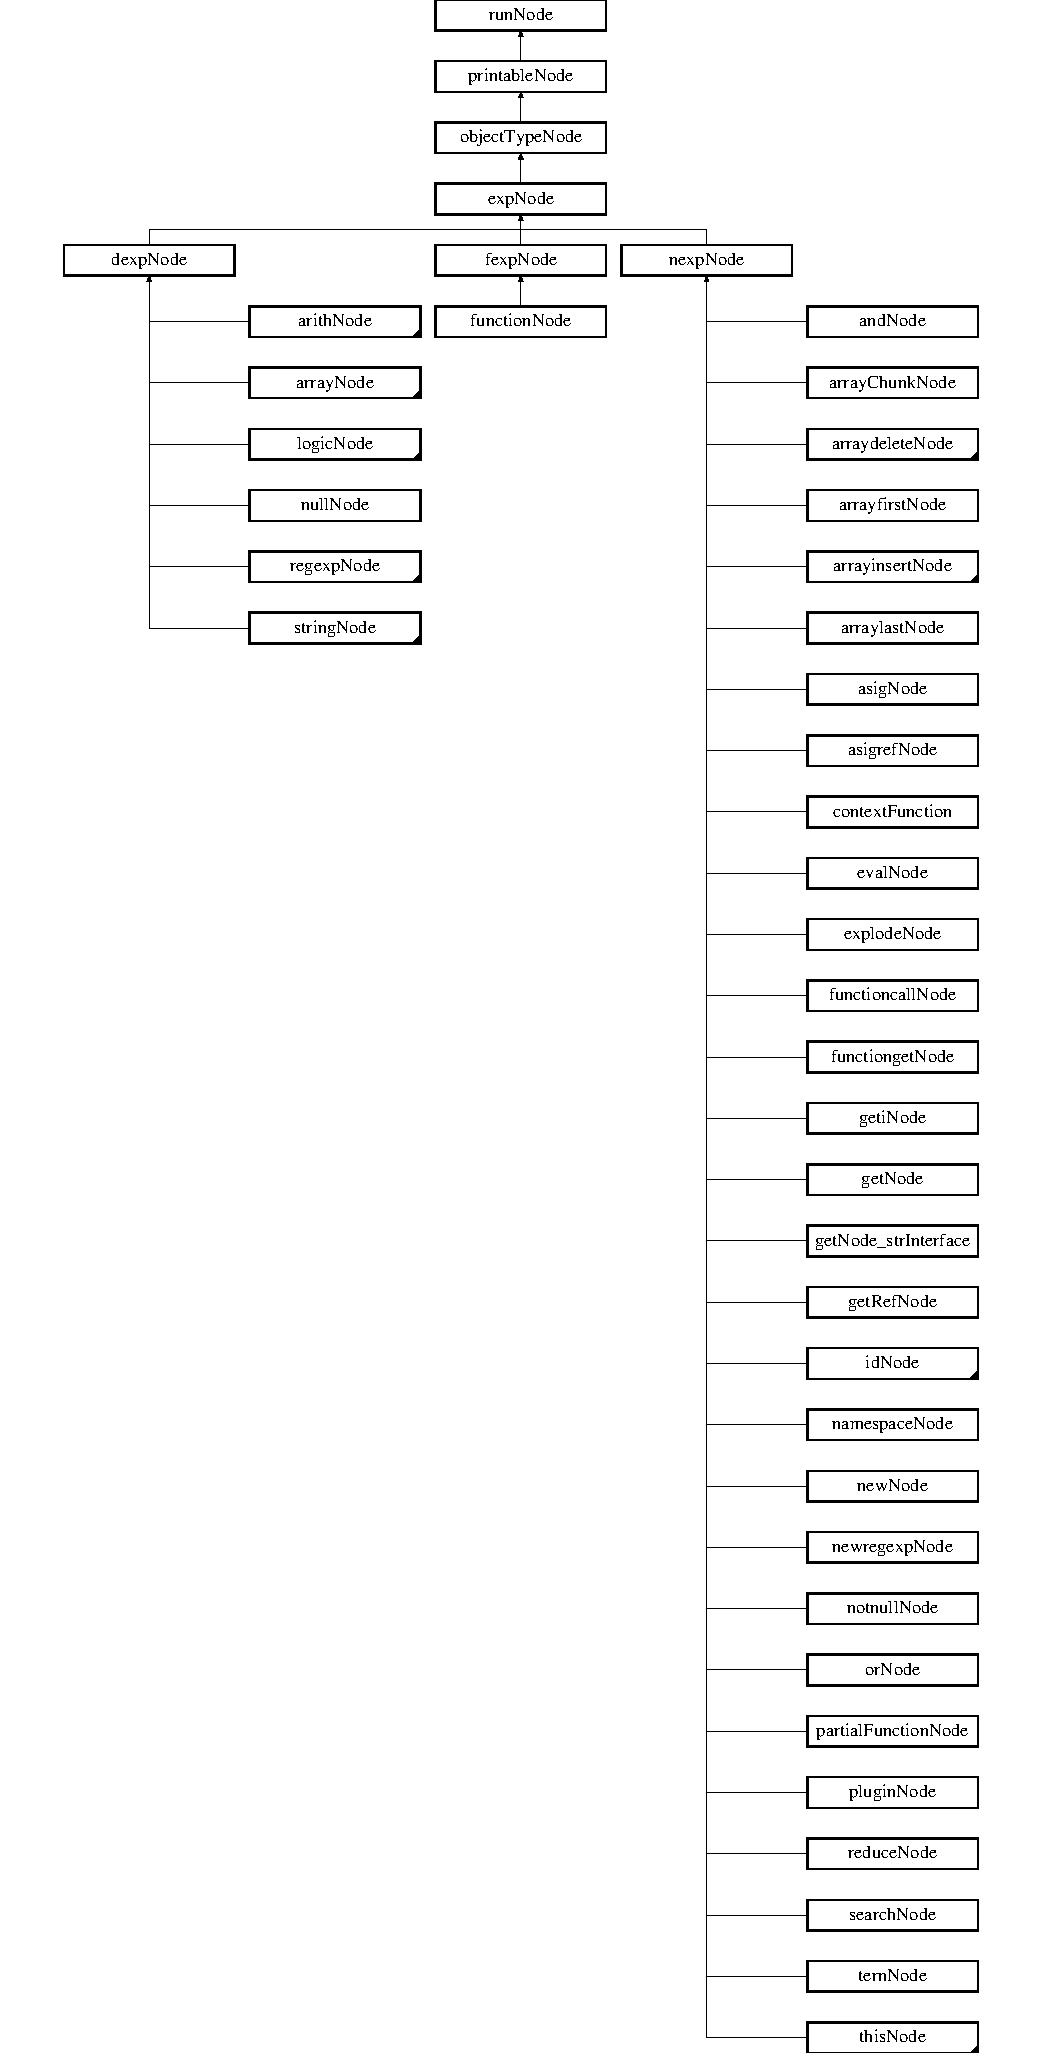
\includegraphics[height=12.000000cm]{classexpNode}
\end{center}
\end{figure}
\subsection*{Métodos públicos}
\begin{DoxyCompactItemize}
\item 
virtual void \hyperlink{classexpNode_aedb96104889212bae315a6381f8e0219}{set\-Node\-Value} (\hyperlink{classrunNode}{run\-Node} $\ast$node)
\end{DoxyCompactItemize}
\subsection*{Métodos públicos estáticos}
\begin{DoxyCompactItemize}
\item 
static \hyperlink{classrunNode}{run\-Node} $\ast$ \hyperlink{classexpNode_aa3d0a7a138a2fc089232f9fadf33a629}{clone} (\hyperlink{classrunNode}{run\-Node} $\ast$node)
\end{DoxyCompactItemize}


\subsection{Descripción detallada}
Nodo de expresión. 

Una expresión tiene asociado un valor resultado de su evaluación.

Los nodos expresiones pueden ser de dos tipos\-:


\begin{DoxyItemize}
\item Definidos (\hyperlink{classdexpNode}{dexp\-Node})\-: Tienen un valor interno definido. Por ejemplo un \hyperlink{classstringNode}{string\-Node} se representa mediante un string.
\item No definidos (\hyperlink{classnexpNode}{nexp\-Node})\-: Tienen un valor interno no definido, haciendo referencia a un nodo ejecutable. Por ejemplo, una expresión de asignación tomará una referencia al nodo asignado, este valor puede ser string, array ....
\end{DoxyItemize}

Los nodos expresión son la base de muchos otros nodos que representan datos, operadores... Estos nodos serán utilizados como parte de una sentencia. 

\subsection{Documentación de las funciones miembro}
\hypertarget{classexpNode_aa3d0a7a138a2fc089232f9fadf33a629}{\index{exp\-Node@{exp\-Node}!clone@{clone}}
\index{clone@{clone}!expNode@{exp\-Node}}
\subsubsection[{clone}]{\setlength{\rightskip}{0pt plus 5cm}{\bf run\-Node} $\ast$ exp\-Node\-::clone (
\begin{DoxyParamCaption}
\item[{{\bf run\-Node} $\ast$}]{node}
\end{DoxyParamCaption}
)\hspace{0.3cm}{\ttfamily [static]}}}\label{classexpNode_aa3d0a7a138a2fc089232f9fadf33a629}
Método que toma un nodo y lo clona en función de su tipo. 
\begin{DoxyParams}{Parámetros}
{\em node} & Nodo a clonar. \\
\hline
\end{DoxyParams}
\begin{DoxyReturn}{Devuelve}
Nodo nuevo. 
\end{DoxyReturn}
\hypertarget{classexpNode_aedb96104889212bae315a6381f8e0219}{\index{exp\-Node@{exp\-Node}!set\-Node\-Value@{set\-Node\-Value}}
\index{set\-Node\-Value@{set\-Node\-Value}!expNode@{exp\-Node}}
\subsubsection[{set\-Node\-Value}]{\setlength{\rightskip}{0pt plus 5cm}void exp\-Node\-::set\-Node\-Value (
\begin{DoxyParamCaption}
\item[{{\bf run\-Node} $\ast$}]{node}
\end{DoxyParamCaption}
)\hspace{0.3cm}{\ttfamily [virtual]}}}\label{classexpNode_aedb96104889212bae315a6381f8e0219}
Establece el valor del nodo. Este método puede ser escrito en los nodos derivados. 
\begin{DoxyParams}{Parámetros}
{\em node} & Nodo que se toma como valor. \\
\hline
\end{DoxyParams}


Reimplementado en \hyperlink{classstringNode_af8d6ed0d5b9be3db1c7be9a905c25f67}{string\-Node}, \hyperlink{classarithNode_aa10435f1e329336baee9334df7a8b0cf}{arith\-Node} y \hyperlink{classlogicNode_a6d3f6e8397d9d0b51b97d681b8380342}{logic\-Node}.



La documentación para esta clase fue generada a partir de los siguientes ficheros\-:\begin{DoxyCompactItemize}
\item 
trunk/src/run/tree/\hyperlink{expNode_8h}{exp\-Node.\-h}\item 
trunk/src/run/tree/exp\-Node.\-cpp\end{DoxyCompactItemize}

\hypertarget{classfappendNode}{\section{Referencia de la Clase fappend\-Node}
\label{classfappendNode}\index{fappend\-Node@{fappend\-Node}}
}


Nodo función añadir a fichero .  




{\ttfamily \#include $<$file\-Op\-Node.\-h$>$}

Diagrama de herencias de fappend\-Node\begin{figure}[H]
\begin{center}
\leavevmode
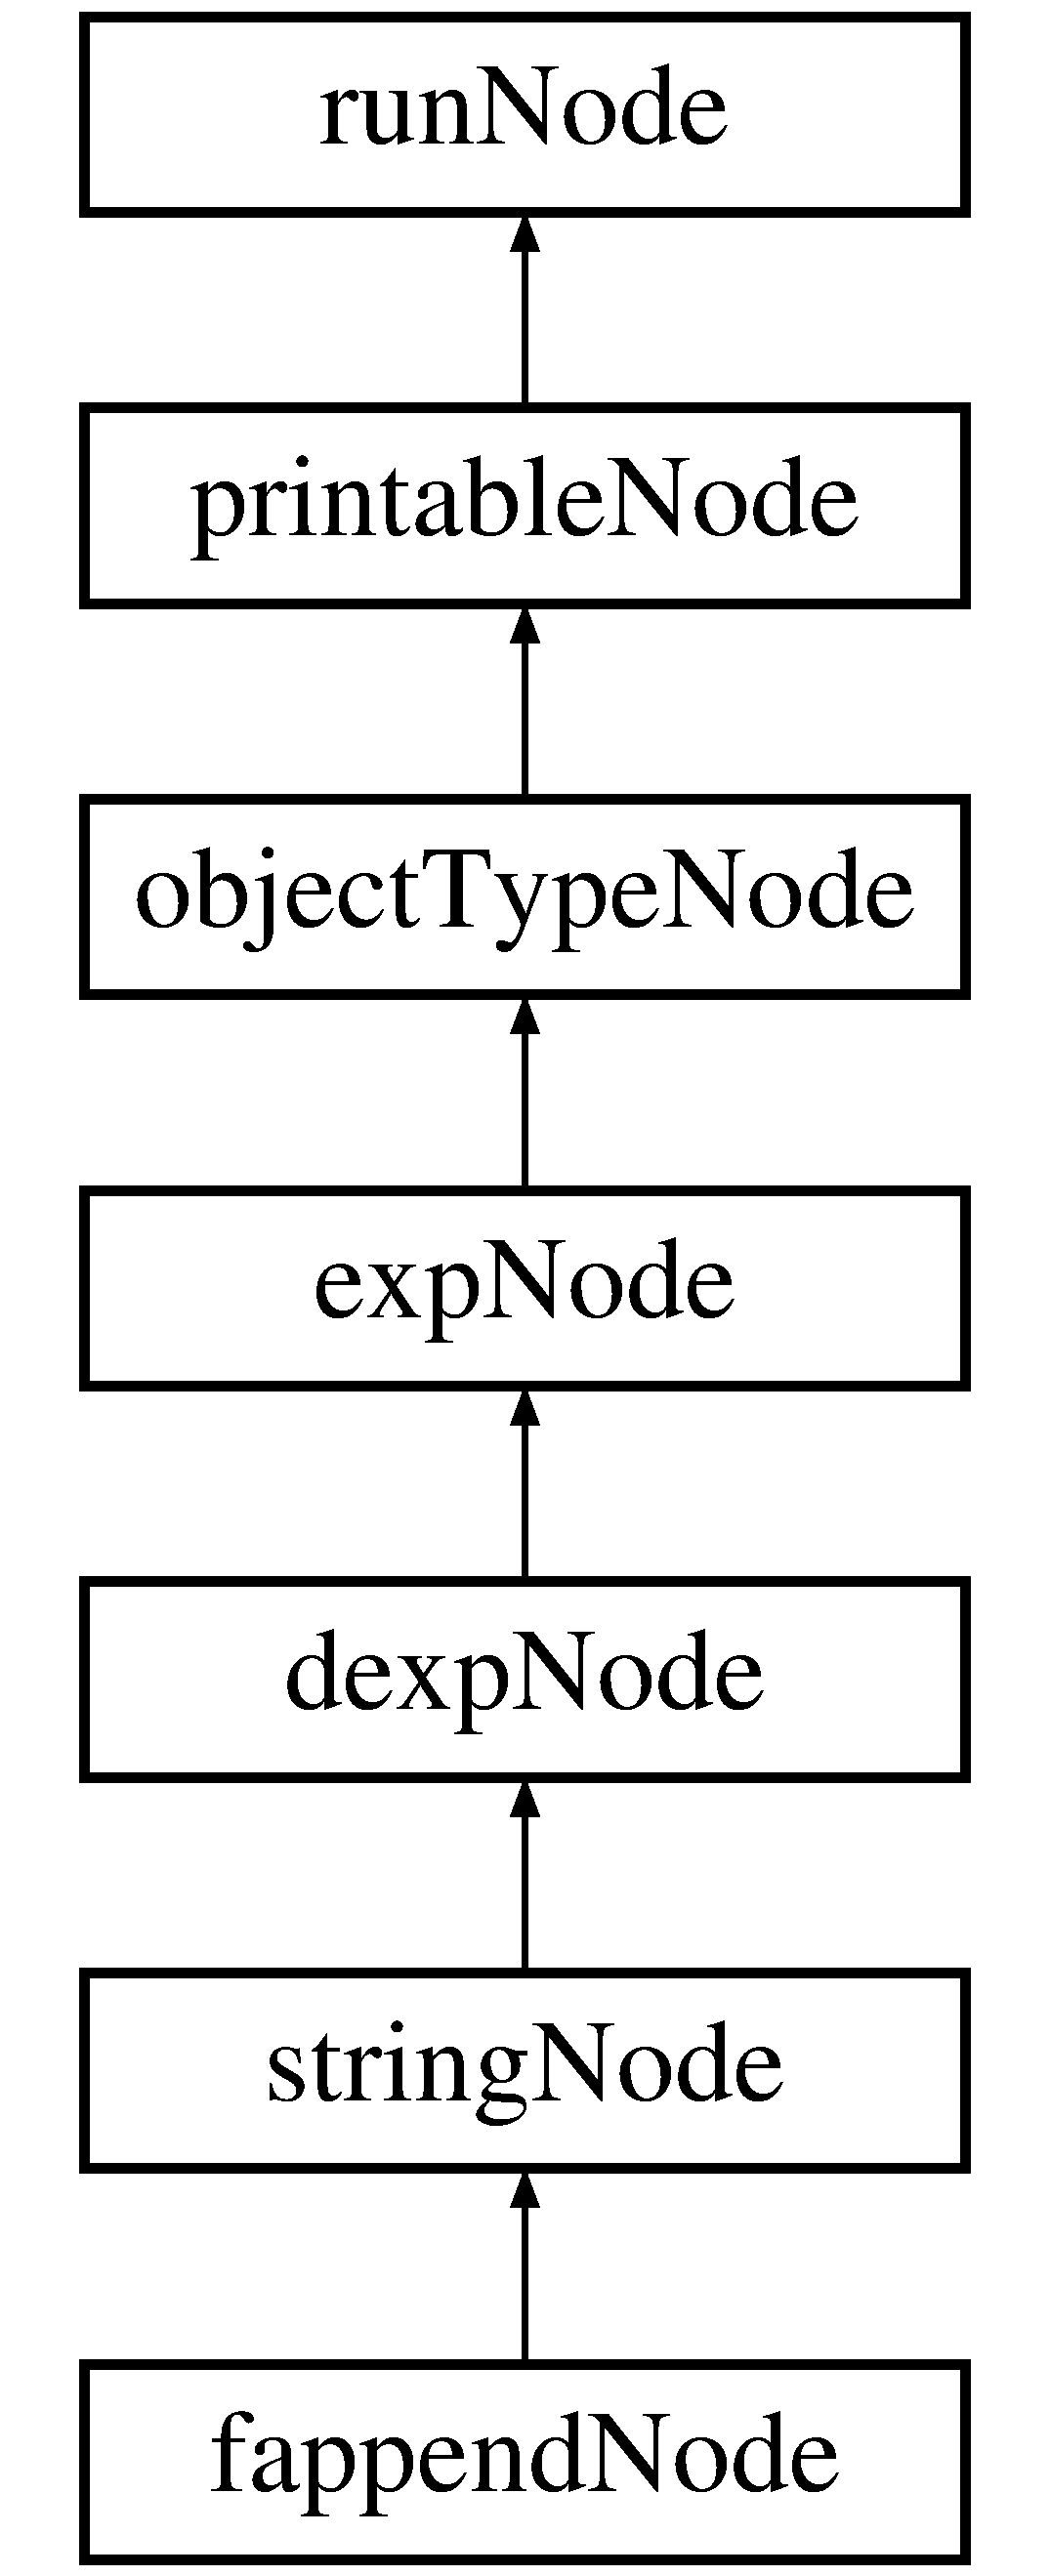
\includegraphics[height=7.000000cm]{classfappendNode}
\end{center}
\end{figure}
\subsection*{Métodos públicos}
\begin{DoxyCompactItemize}
\item 
\hyperlink{classfappendNode_a7cd57233e2f352716a011cc770999ef9}{fappend\-Node} (\hyperlink{classrunNode}{run\-Node} $\ast$file, \hyperlink{classrunNode}{run\-Node} $\ast$str)
\item 
void \hyperlink{classfappendNode_a872c68dabc8306cc405452ce4200b7bd}{run} ()
\end{DoxyCompactItemize}
\subsection*{Otros miembros heredados}


\subsection{Descripción detallada}
Nodo función añadir a fichero . 

Escribe una cadena de caracteres al final de un fichero. 

\subsection{Documentación del constructor y destructor}
\hypertarget{classfappendNode_a7cd57233e2f352716a011cc770999ef9}{\index{fappend\-Node@{fappend\-Node}!fappend\-Node@{fappend\-Node}}
\index{fappend\-Node@{fappend\-Node}!fappendNode@{fappend\-Node}}
\subsubsection[{fappend\-Node}]{\setlength{\rightskip}{0pt plus 5cm}fappend\-Node\-::fappend\-Node (
\begin{DoxyParamCaption}
\item[{{\bf run\-Node} $\ast$}]{file, }
\item[{{\bf run\-Node} $\ast$}]{str}
\end{DoxyParamCaption}
)}}\label{classfappendNode_a7cd57233e2f352716a011cc770999ef9}
Constructor de la clase. 
\begin{DoxyParams}{Parámetros}
{\em file.} & Nodo que representa la ruta del fichero en el que se escribirá. \\
\hline
{\em str.} & Nodo que representa la cadena que se escribirá \\
\hline
\end{DoxyParams}


\subsection{Documentación de las funciones miembro}
\hypertarget{classfappendNode_a872c68dabc8306cc405452ce4200b7bd}{\index{fappend\-Node@{fappend\-Node}!run@{run}}
\index{run@{run}!fappendNode@{fappend\-Node}}
\subsubsection[{run}]{\setlength{\rightskip}{0pt plus 5cm}void fappend\-Node\-::run (
\begin{DoxyParamCaption}
{}
\end{DoxyParamCaption}
)\hspace{0.3cm}{\ttfamily [virtual]}}}\label{classfappendNode_a872c68dabc8306cc405452ce4200b7bd}
Método de ejecución. Añade la cadena al final de un fichero. Si el fichero no existe es creado. Como valor toma la cadena escrita. 

Implementa \hyperlink{classrunNode_a83c10df8148829b08e04153c93d69eec}{run\-Node}.



La documentación para esta clase fue generada a partir de los siguientes ficheros\-:\begin{DoxyCompactItemize}
\item 
trunk/src/run/operators/\hyperlink{fileOpNode_8h}{file\-Op\-Node.\-h}\item 
trunk/src/run/operators/file\-Op\-Node.\-cpp\end{DoxyCompactItemize}

\hypertarget{classfcloseNode}{\section{Referencia de la Clase fclose\-Node}
\label{classfcloseNode}\index{fclose\-Node@{fclose\-Node}}
}


Nodo función que cierra un descriptor de fichero.  




{\ttfamily \#include $<$file\-Op\-Node.\-h$>$}

Diagrama de herencias de fclose\-Node\begin{figure}[H]
\begin{center}
\leavevmode
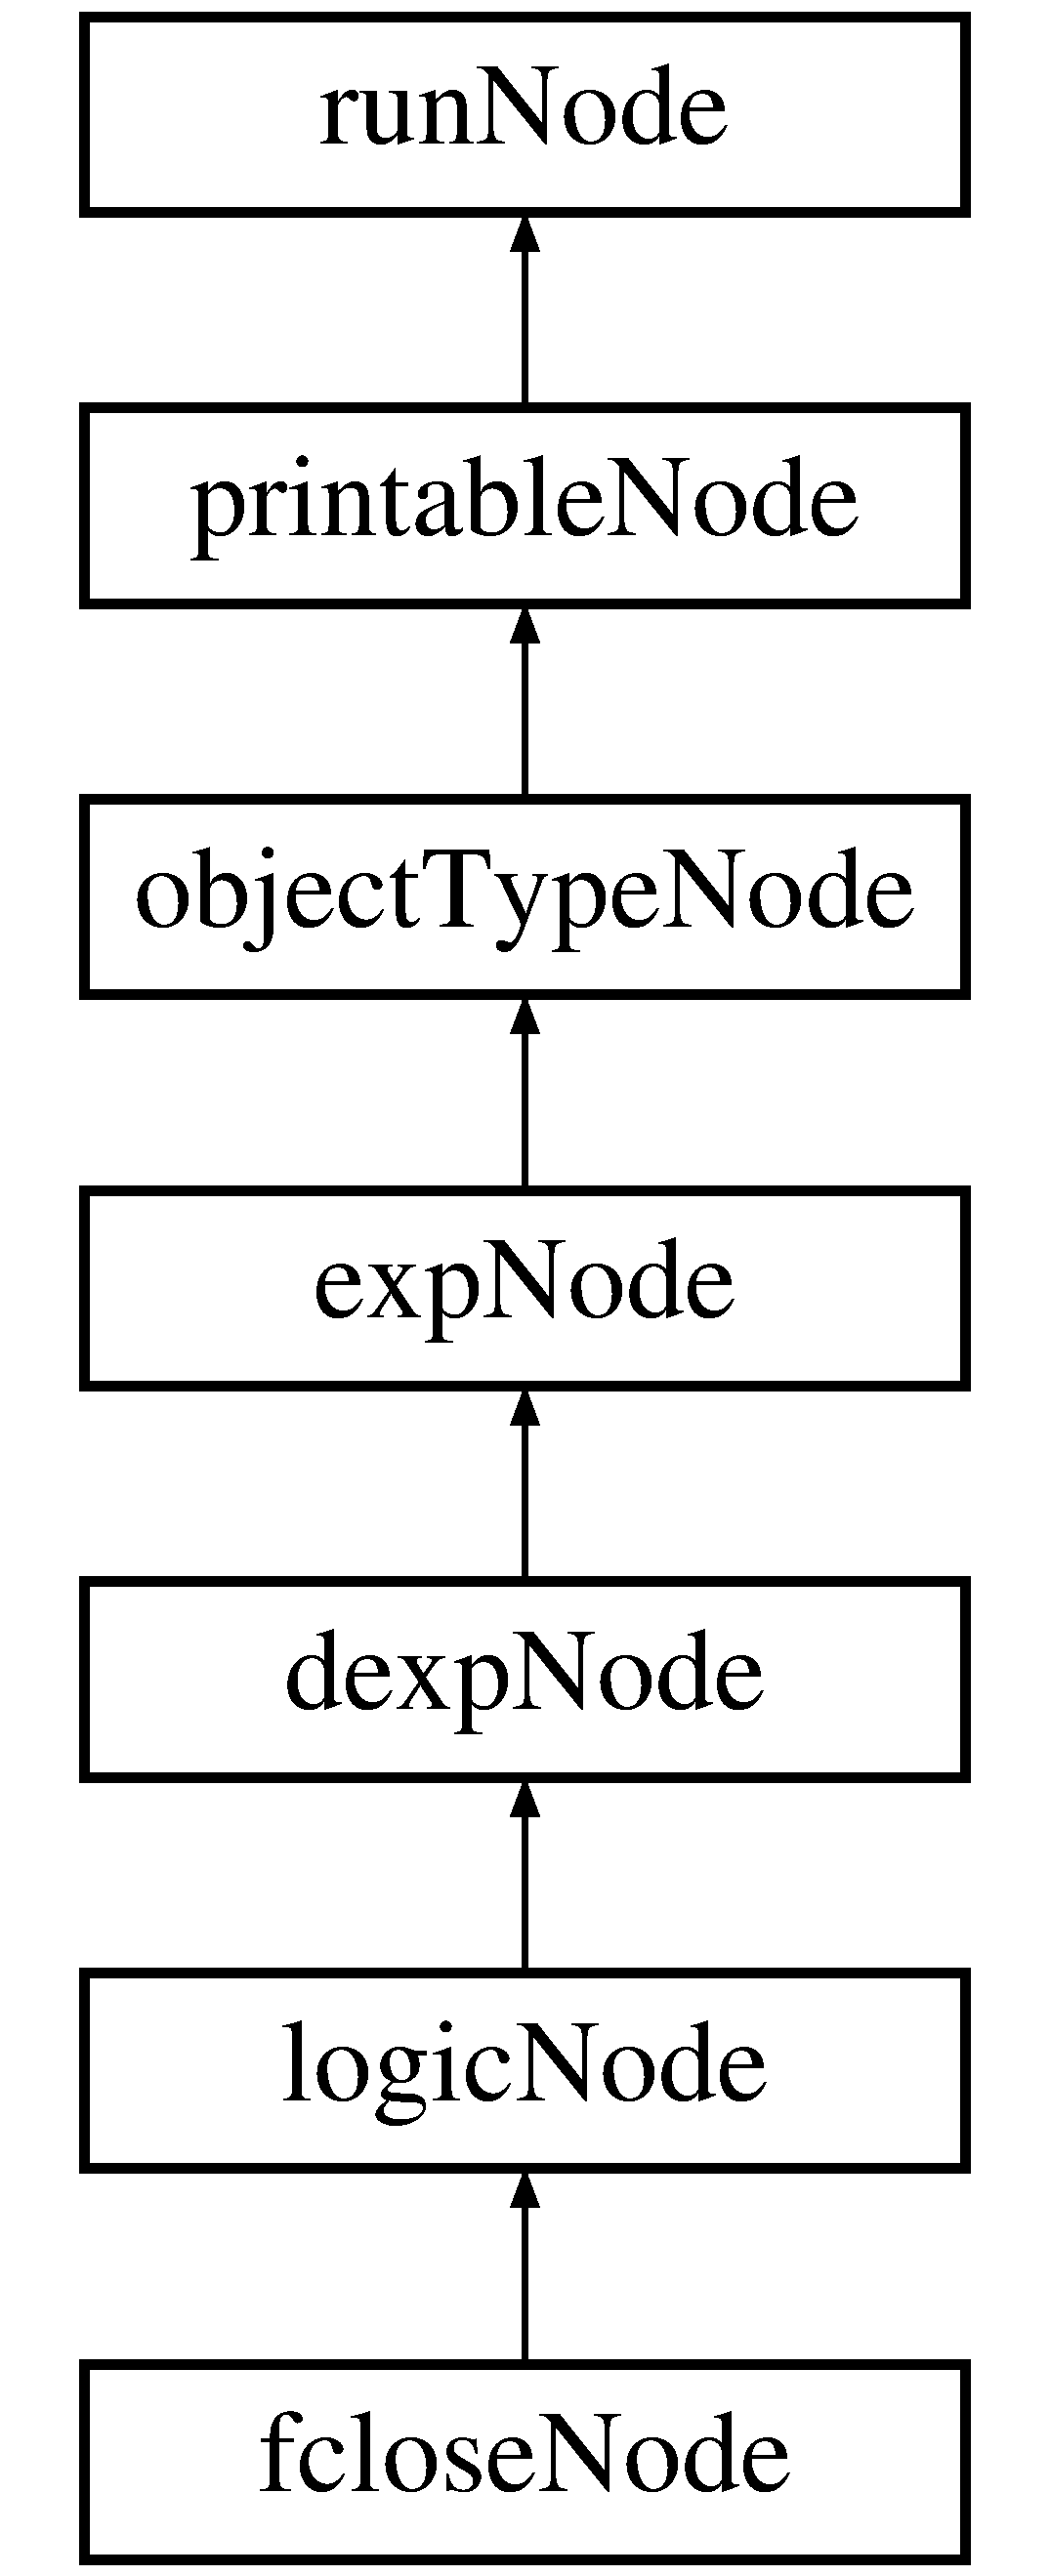
\includegraphics[height=7.000000cm]{classfcloseNode}
\end{center}
\end{figure}
\subsection*{Métodos públicos}
\begin{DoxyCompactItemize}
\item 
\hyperlink{classfcloseNode_aebf6497162cd14d57fc18151d02e231d}{fclose\-Node} (\hyperlink{classrunNode}{run\-Node} $\ast$file)
\item 
void \hyperlink{classfcloseNode_a6110a473ad462d640df0095c9c3764dd}{run} ()
\end{DoxyCompactItemize}
\subsection*{Otros miembros heredados}


\subsection{Descripción detallada}
Nodo función que cierra un descriptor de fichero. 

La ejecución de este nodo conlleva el cierre de un descriptor de fichero. 

\subsection{Documentación del constructor y destructor}
\hypertarget{classfcloseNode_aebf6497162cd14d57fc18151d02e231d}{\index{fclose\-Node@{fclose\-Node}!fclose\-Node@{fclose\-Node}}
\index{fclose\-Node@{fclose\-Node}!fcloseNode@{fclose\-Node}}
\subsubsection[{fclose\-Node}]{\setlength{\rightskip}{0pt plus 5cm}fclose\-Node\-::fclose\-Node (
\begin{DoxyParamCaption}
\item[{{\bf run\-Node} $\ast$}]{file}
\end{DoxyParamCaption}
)}}\label{classfcloseNode_aebf6497162cd14d57fc18151d02e231d}
Constructor de la clase. 
\begin{DoxyParams}{Parámetros}
{\em file.} & Nodo que representa el descriptor de fichero \\
\hline
\end{DoxyParams}


\subsection{Documentación de las funciones miembro}
\hypertarget{classfcloseNode_a6110a473ad462d640df0095c9c3764dd}{\index{fclose\-Node@{fclose\-Node}!run@{run}}
\index{run@{run}!fcloseNode@{fclose\-Node}}
\subsubsection[{run}]{\setlength{\rightskip}{0pt plus 5cm}void fclose\-Node\-::run (
\begin{DoxyParamCaption}
{}
\end{DoxyParamCaption}
)\hspace{0.3cm}{\ttfamily [virtual]}}}\label{classfcloseNode_a6110a473ad462d640df0095c9c3764dd}
Método de ejecución. Procede a cerrar el descriptor de fichero finalizando todas las operaciones pendientes. Toma como valor un booleano que indica si el proceso se llevó a cabo correctamente. 

Implementa \hyperlink{classrunNode_a83c10df8148829b08e04153c93d69eec}{run\-Node}.



La documentación para esta clase fue generada a partir de los siguientes ficheros\-:\begin{DoxyCompactItemize}
\item 
trunk/src/run/operators/\hyperlink{fileOpNode_8h}{file\-Op\-Node.\-h}\item 
trunk/src/run/operators/file\-Op\-Node.\-cpp\end{DoxyCompactItemize}

\hypertarget{classfexpNode}{\section{Referencia de la Clase fexp\-Node}
\label{classfexpNode}\index{fexp\-Node@{fexp\-Node}}
}


Nodo expresiones funciones.  




{\ttfamily \#include $<$exp\-Node.\-h$>$}

Diagrama de herencias de fexp\-Node\begin{figure}[H]
\begin{center}
\leavevmode
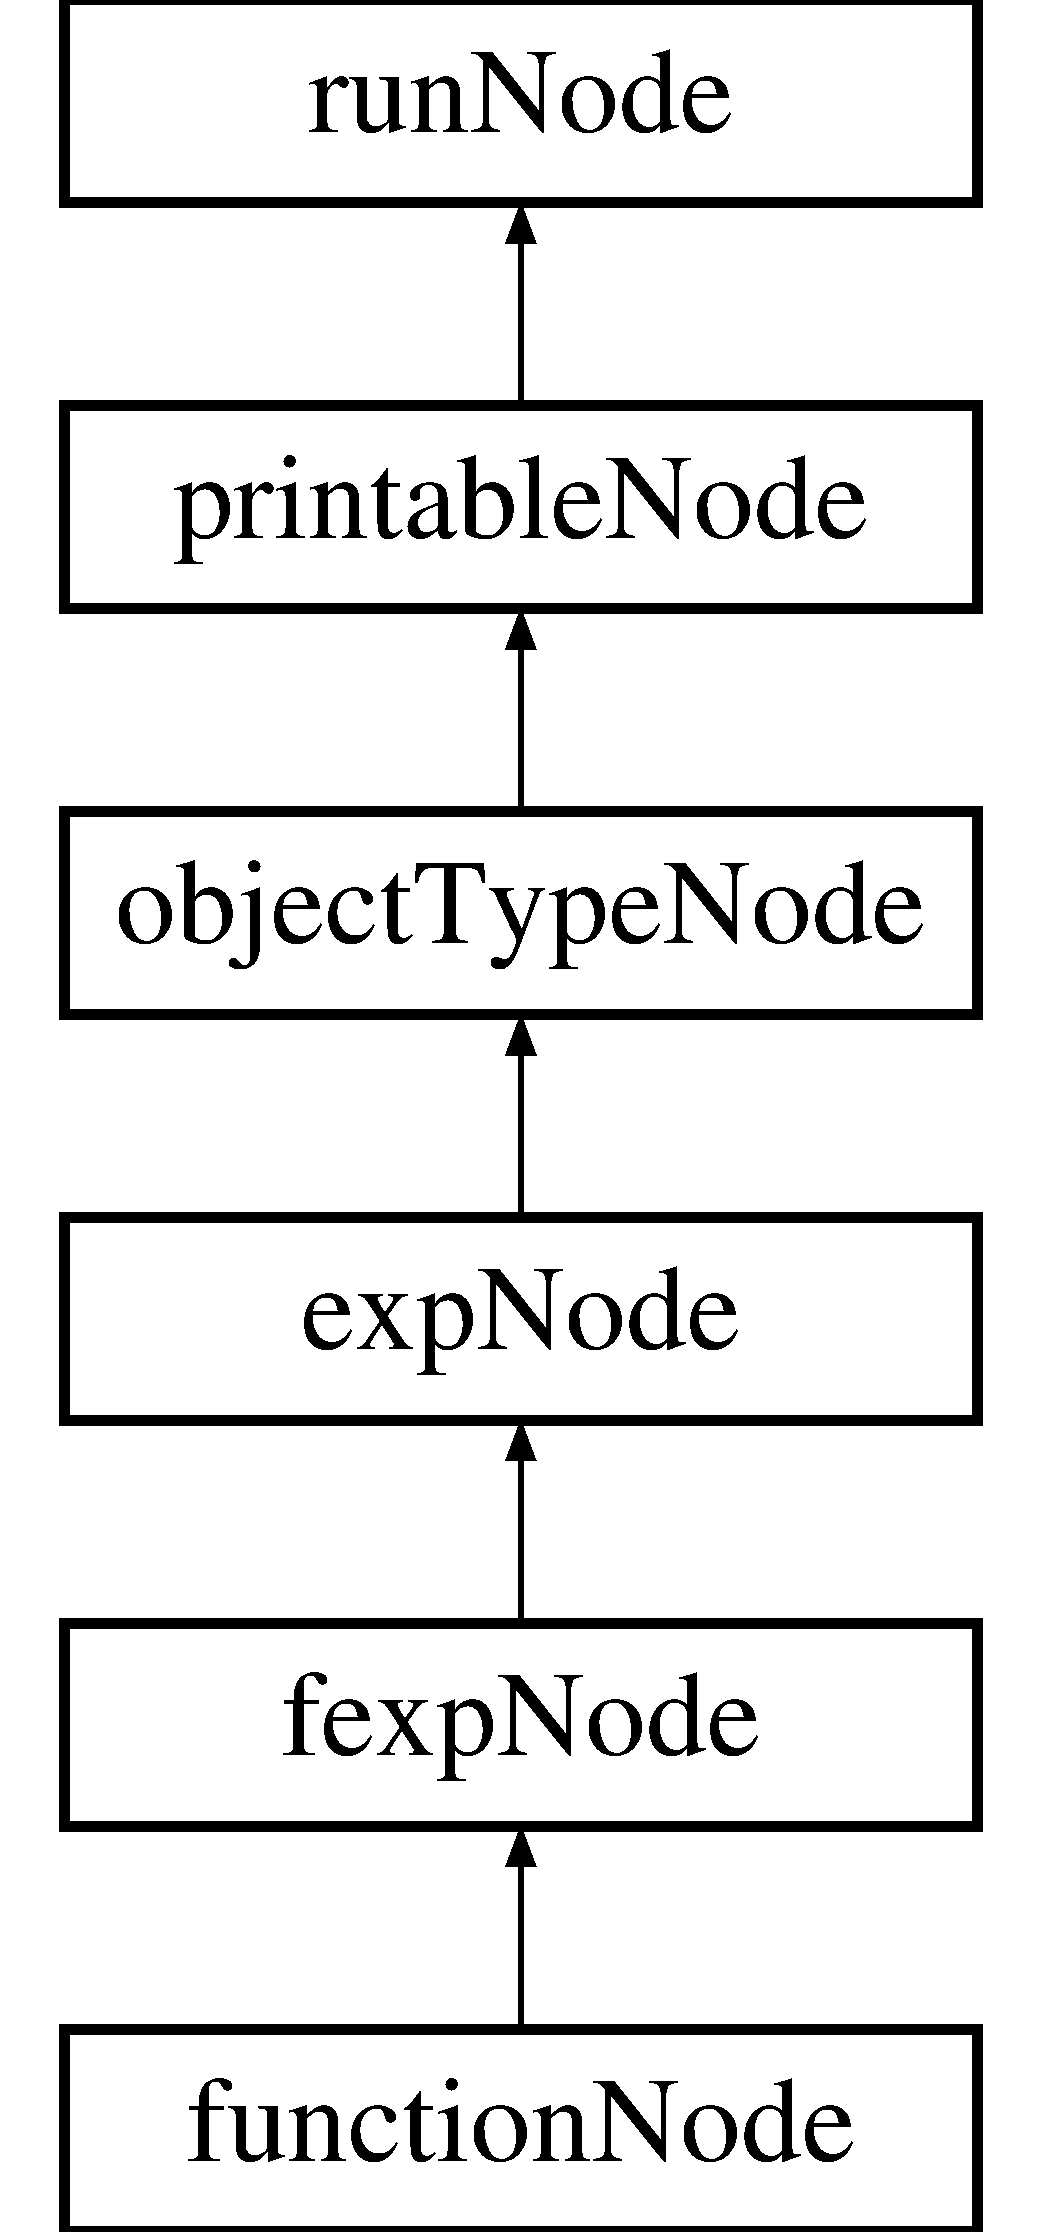
\includegraphics[height=6.000000cm]{classfexpNode}
\end{center}
\end{figure}
\subsection*{Métodos públicos}
\begin{DoxyCompactItemize}
\item 
bool \hyperlink{classfexpNode_af28c9cdf9743d074f40b7dbb1f51efbb}{is\-\_\-print} () const 
\item 
bool \hyperlink{classfexpNode_a325f796b4c98dbd3453cdb1fd298b53d}{is\-\_\-runlist} () const 
\item 
void \hyperlink{classfexpNode_a26cdef5bf8cd58af7e9955b74350c48b}{rm\-Ref} ()
\end{DoxyCompactItemize}
\subsection*{Otros miembros heredados}


\subsection{Descripción detallada}
Nodo expresiones funciones. 

Define nodos que representan expresiones formadas mediante la declaración de funciones. 

\subsection{Documentación de las funciones miembro}
\hypertarget{classfexpNode_af28c9cdf9743d074f40b7dbb1f51efbb}{\index{fexp\-Node@{fexp\-Node}!is\-\_\-print@{is\-\_\-print}}
\index{is\-\_\-print@{is\-\_\-print}!fexpNode@{fexp\-Node}}
\subsubsection[{is\-\_\-print}]{\setlength{\rightskip}{0pt plus 5cm}bool fexp\-Node\-::is\-\_\-print (
\begin{DoxyParamCaption}
{}
\end{DoxyParamCaption}
) const\hspace{0.3cm}{\ttfamily [virtual]}}}\label{classfexpNode_af28c9cdf9743d074f40b7dbb1f51efbb}
Una función no es imprimible. \begin{DoxyReturn}{Devuelve}
Falso 
\end{DoxyReturn}


Reimplementado de \hyperlink{classrunNode_ad65c9a22e807dbe18f5c83c84d777d44}{run\-Node}.

\hypertarget{classfexpNode_a325f796b4c98dbd3453cdb1fd298b53d}{\index{fexp\-Node@{fexp\-Node}!is\-\_\-runlist@{is\-\_\-runlist}}
\index{is\-\_\-runlist@{is\-\_\-runlist}!fexpNode@{fexp\-Node}}
\subsubsection[{is\-\_\-runlist}]{\setlength{\rightskip}{0pt plus 5cm}bool fexp\-Node\-::is\-\_\-runlist (
\begin{DoxyParamCaption}
{}
\end{DoxyParamCaption}
) const\hspace{0.3cm}{\ttfamily [virtual]}}}\label{classfexpNode_a325f796b4c98dbd3453cdb1fd298b53d}
Una función no es un elemento de lista. \begin{DoxyReturn}{Devuelve}
Falso 
\end{DoxyReturn}


Reimplementado de \hyperlink{classrunNode_a231638d0fc5b436c5e4a664fe7d5126a}{run\-Node}.

\hypertarget{classfexpNode_a26cdef5bf8cd58af7e9955b74350c48b}{\index{fexp\-Node@{fexp\-Node}!rm\-Ref@{rm\-Ref}}
\index{rm\-Ref@{rm\-Ref}!fexpNode@{fexp\-Node}}
\subsubsection[{rm\-Ref}]{\setlength{\rightskip}{0pt plus 5cm}void fexp\-Node\-::rm\-Ref (
\begin{DoxyParamCaption}
{}
\end{DoxyParamCaption}
)\hspace{0.3cm}{\ttfamily [virtual]}}}\label{classfexpNode_a26cdef5bf8cd58af7e9955b74350c48b}
Una función no puede ser eliminada de la formal normal. 

Reimplementado de \hyperlink{classrunNode_a8d0761660753ceb2c98836614c526a45}{run\-Node}.



La documentación para esta clase fue generada a partir de los siguientes ficheros\-:\begin{DoxyCompactItemize}
\item 
trunk/src/run/tree/\hyperlink{expNode_8h}{exp\-Node.\-h}\item 
trunk/src/run/tree/exp\-Node.\-cpp\end{DoxyCompactItemize}

\hypertarget{classfgetNode}{\section{Referencia de la Clase fget\-Node}
\label{classfgetNode}\index{fget\-Node@{fget\-Node}}
}


Nodo función leer de descriptor de fichero.  




{\ttfamily \#include $<$file\-Op\-Node.\-h$>$}

Diagrama de herencias de fget\-Node\begin{figure}[H]
\begin{center}
\leavevmode
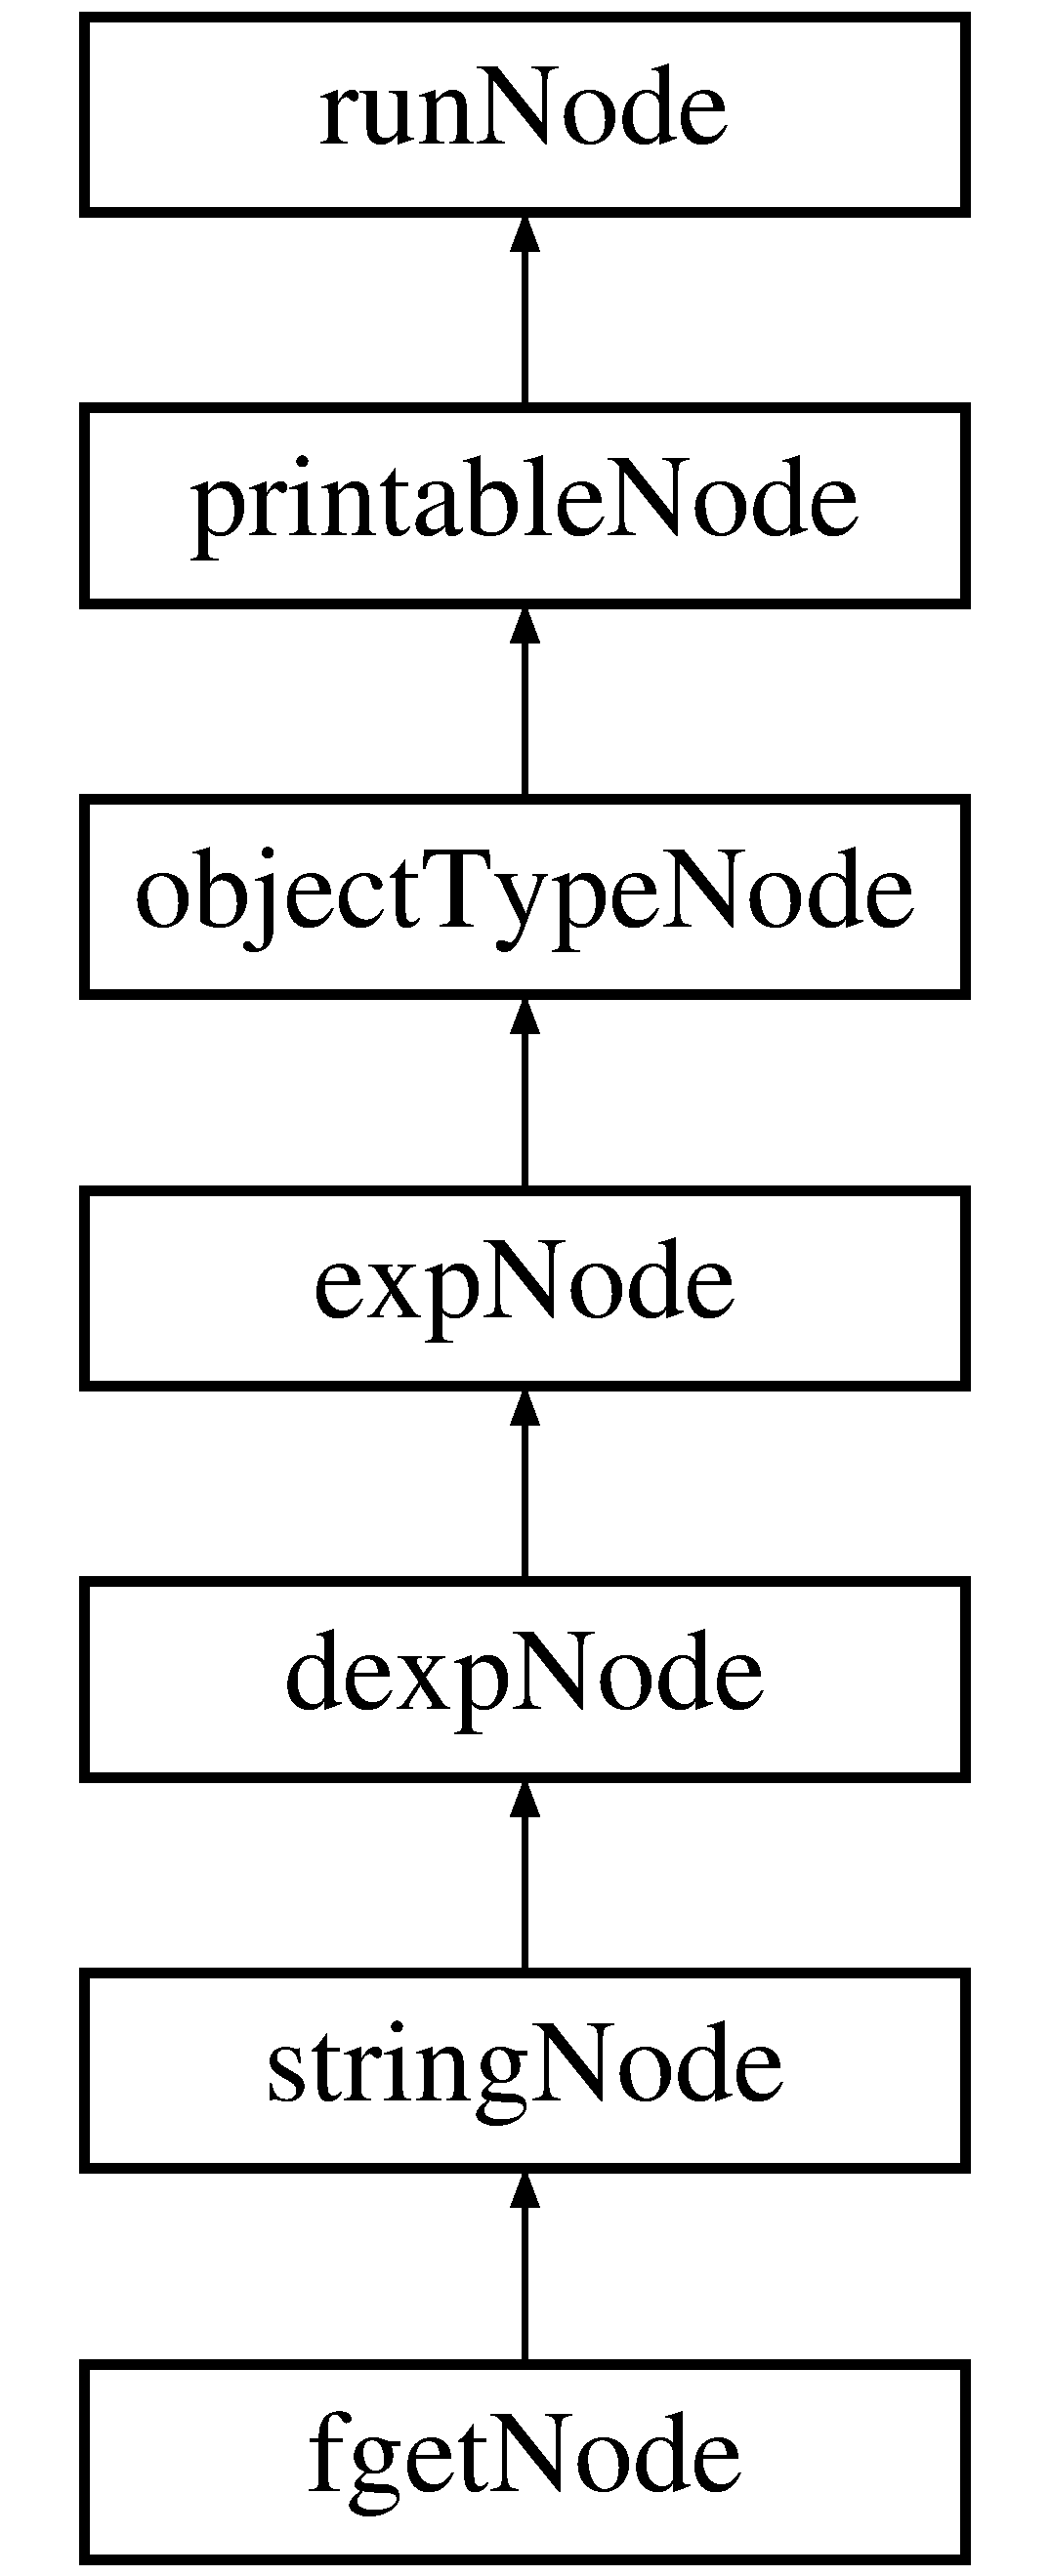
\includegraphics[height=7.000000cm]{classfgetNode}
\end{center}
\end{figure}
\subsection*{Métodos públicos}
\begin{DoxyCompactItemize}
\item 
\hyperlink{classfgetNode_a4d97f7eadb024edf1608a74598d5e472}{fget\-Node} (\hyperlink{classrunNode}{run\-Node} $\ast$file, \hyperlink{classrunNode}{run\-Node} $\ast$size=N\-U\-L\-L)
\item 
void \hyperlink{classfgetNode_a189fa91cf346d112382c333348d1ffcd}{run} ()
\end{DoxyCompactItemize}
\subsection*{Otros miembros heredados}


\subsection{Descripción detallada}
Nodo función leer de descriptor de fichero. 

Este nodo se encarga de leer desde la posición en la que se encuentra un descriptor de fichero un número de caracteres. 

\subsection{Documentación del constructor y destructor}
\hypertarget{classfgetNode_a4d97f7eadb024edf1608a74598d5e472}{\index{fget\-Node@{fget\-Node}!fget\-Node@{fget\-Node}}
\index{fget\-Node@{fget\-Node}!fgetNode@{fget\-Node}}
\subsubsection[{fget\-Node}]{\setlength{\rightskip}{0pt plus 5cm}fget\-Node\-::fget\-Node (
\begin{DoxyParamCaption}
\item[{{\bf run\-Node} $\ast$}]{file, }
\item[{{\bf run\-Node} $\ast$}]{size = {\ttfamily NULL}}
\end{DoxyParamCaption}
)}}\label{classfgetNode_a4d97f7eadb024edf1608a74598d5e472}
Constructor de la clase. 
\begin{DoxyParams}{Parámetros}
{\em file.} & Nodo descriptor de fichero \\
\hline
{\em size.} & Nodo que representa el número de caracteres que serán leídos. Si no es dado se toma hasta el siguiente salto de línea. \\
\hline
\end{DoxyParams}


\subsection{Documentación de las funciones miembro}
\hypertarget{classfgetNode_a189fa91cf346d112382c333348d1ffcd}{\index{fget\-Node@{fget\-Node}!run@{run}}
\index{run@{run}!fgetNode@{fget\-Node}}
\subsubsection[{run}]{\setlength{\rightskip}{0pt plus 5cm}void fget\-Node\-::run (
\begin{DoxyParamCaption}
{}
\end{DoxyParamCaption}
)\hspace{0.3cm}{\ttfamily [virtual]}}}\label{classfgetNode_a189fa91cf346d112382c333348d1ffcd}
Método de ejecución. Lee del fichero el número de caracteres establecidos. Toma como valor la cadena leída. 

Implementa \hyperlink{classrunNode_a83c10df8148829b08e04153c93d69eec}{run\-Node}.



La documentación para esta clase fue generada a partir de los siguientes ficheros\-:\begin{DoxyCompactItemize}
\item 
trunk/src/run/operators/\hyperlink{fileOpNode_8h}{file\-Op\-Node.\-h}\item 
trunk/src/run/operators/file\-Op\-Node.\-cpp\end{DoxyCompactItemize}

\hypertarget{classfileNode}{\section{Referencia de la Clase file\-Node}
\label{classfileNode}\index{file\-Node@{file\-Node}}
}


Nodo fichero .  




{\ttfamily \#include $<$file\-Op\-Node.\-h$>$}

Diagrama de herencias de file\-Node\begin{figure}[H]
\begin{center}
\leavevmode
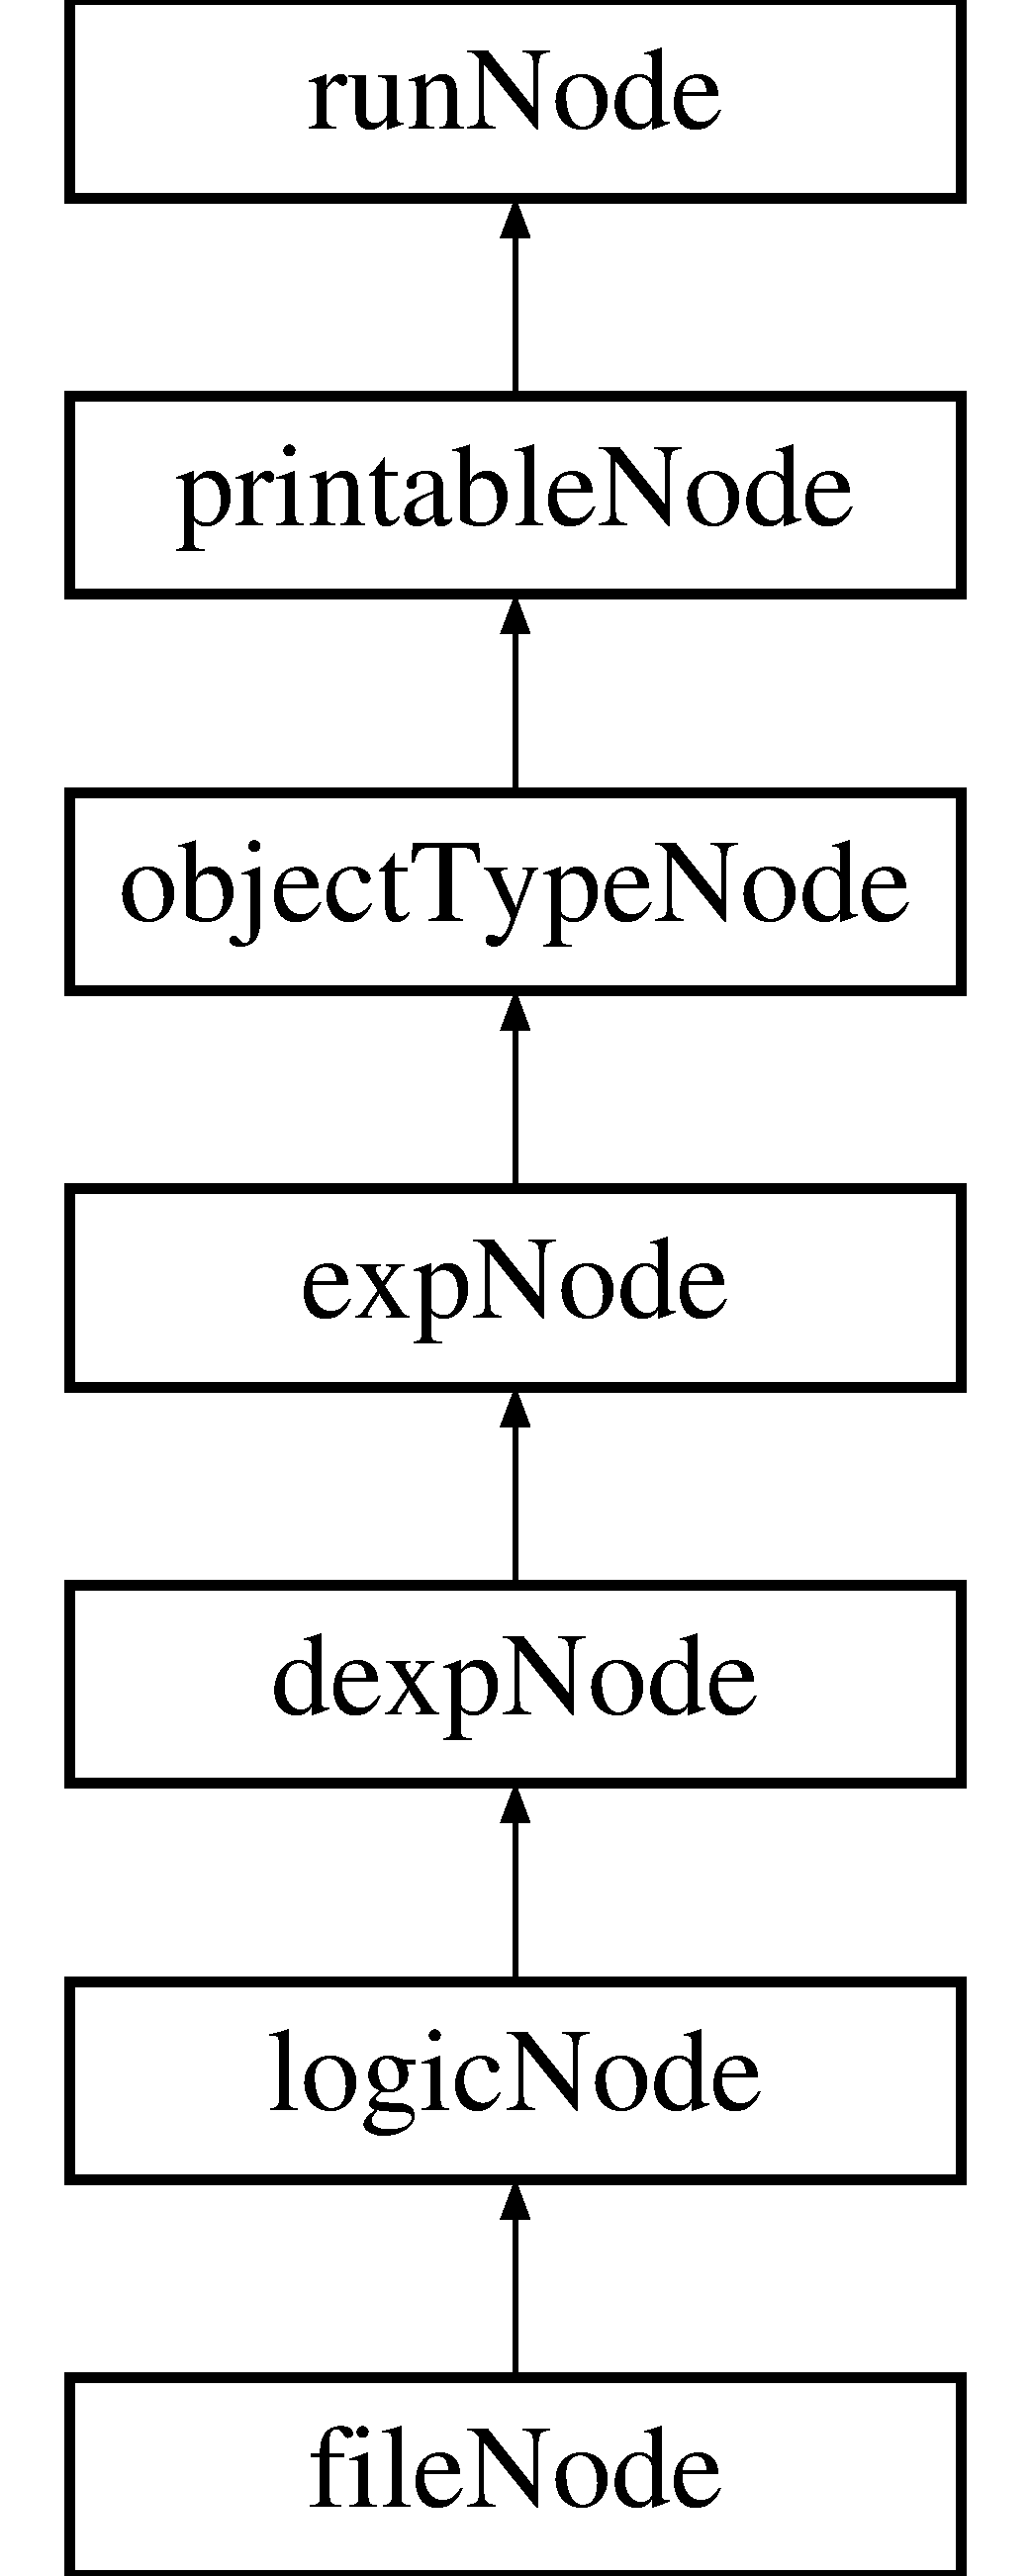
\includegraphics[height=7.000000cm]{classfileNode}
\end{center}
\end{figure}
\subsection*{Métodos públicos}
\begin{DoxyCompactItemize}
\item 
\hyperlink{classfileNode_a2d9014c5f0902bd415b41a6519056c4b}{file\-Node} (\hyperlink{classrunNode}{run\-Node} $\ast$file, \hyperlink{classrunNode}{run\-Node} $\ast$mode=N\-U\-L\-L)
\item 
void \hyperlink{classfileNode_a54a9c6df980993a5de838839f4fc54f3}{run} ()
\item 
fstream $\ast$ \hyperlink{classfileNode_a46be9af6a79c1956c0e07444c2ec713e}{get} () const 
\item 
string \hyperlink{classfileNode_a6b5786f432ddab8daf3c90deb24413c9}{get\-Mode} ()
\end{DoxyCompactItemize}
\subsection*{Otros miembros heredados}


\subsection{Descripción detallada}
Nodo fichero . 

Este nodo abre un descriptor de fichero segun una ruta dada y un modo.

El modo puede ser\-:
\begin{DoxyItemize}
\item r\-: Solo lectura
\item r+\-: Lectura y/o escritura
\item w\-: Escritura truncando el fichero
\item w+\-: Lectura y/o escritura truncando el fichero
\item a\-: Escritura posicionando el puntero al final del fichero
\item a+\-: Lectura y/o escritura posicionando el puntero al final del fichero 
\end{DoxyItemize}

\subsection{Documentación del constructor y destructor}
\hypertarget{classfileNode_a2d9014c5f0902bd415b41a6519056c4b}{\index{file\-Node@{file\-Node}!file\-Node@{file\-Node}}
\index{file\-Node@{file\-Node}!fileNode@{file\-Node}}
\subsubsection[{file\-Node}]{\setlength{\rightskip}{0pt plus 5cm}file\-Node\-::file\-Node (
\begin{DoxyParamCaption}
\item[{{\bf run\-Node} $\ast$}]{file, }
\item[{{\bf run\-Node} $\ast$}]{mode = {\ttfamily NULL}}
\end{DoxyParamCaption}
)}}\label{classfileNode_a2d9014c5f0902bd415b41a6519056c4b}
Constructor de la clase. 
\begin{DoxyParams}{Parámetros}
{\em file.} & Nodo que representa la ruta de un fichero \\
\hline
{\em mode.} & Nodo que representa la cadena que determina el modo \\
\hline
\end{DoxyParams}


\subsection{Documentación de las funciones miembro}
\hypertarget{classfileNode_a46be9af6a79c1956c0e07444c2ec713e}{\index{file\-Node@{file\-Node}!get@{get}}
\index{get@{get}!fileNode@{file\-Node}}
\subsubsection[{get}]{\setlength{\rightskip}{0pt plus 5cm}fstream$\ast$ file\-Node\-::get (
\begin{DoxyParamCaption}
{}
\end{DoxyParamCaption}
) const\hspace{0.3cm}{\ttfamily [inline]}}}\label{classfileNode_a46be9af6a79c1956c0e07444c2ec713e}
Obtiene el descriptor de fichero interno \begin{DoxyReturn}{Devuelve}
Descriptor de fichero 
\end{DoxyReturn}
\hypertarget{classfileNode_a6b5786f432ddab8daf3c90deb24413c9}{\index{file\-Node@{file\-Node}!get\-Mode@{get\-Mode}}
\index{get\-Mode@{get\-Mode}!fileNode@{file\-Node}}
\subsubsection[{get\-Mode}]{\setlength{\rightskip}{0pt plus 5cm}string file\-Node\-::get\-Mode (
\begin{DoxyParamCaption}
{}
\end{DoxyParamCaption}
)\hspace{0.3cm}{\ttfamily [inline]}}}\label{classfileNode_a6b5786f432ddab8daf3c90deb24413c9}
Obtiene el modo \begin{DoxyReturn}{Devuelve}
Cadena correspondiente al modo 
\end{DoxyReturn}
\hypertarget{classfileNode_a54a9c6df980993a5de838839f4fc54f3}{\index{file\-Node@{file\-Node}!run@{run}}
\index{run@{run}!fileNode@{file\-Node}}
\subsubsection[{run}]{\setlength{\rightskip}{0pt plus 5cm}void file\-Node\-::run (
\begin{DoxyParamCaption}
{}
\end{DoxyParamCaption}
)\hspace{0.3cm}{\ttfamily [virtual]}}}\label{classfileNode_a54a9c6df980993a5de838839f4fc54f3}
Método de ejecución. Abre el descriptor de fichero y lo toma como valor. 

Implementa \hyperlink{classrunNode_a83c10df8148829b08e04153c93d69eec}{run\-Node}.



La documentación para esta clase fue generada a partir de los siguientes ficheros\-:\begin{DoxyCompactItemize}
\item 
trunk/src/run/operators/\hyperlink{fileOpNode_8h}{file\-Op\-Node.\-h}\item 
trunk/src/run/operators/file\-Op\-Node.\-cpp\end{DoxyCompactItemize}

\hypertarget{classfindNode}{\section{Referencia de la Clase find\-Node}
\label{classfindNode}\index{find\-Node@{find\-Node}}
}


Nodo función búsqueda de subcadena.  




{\ttfamily \#include $<$str\-Op\-Node.\-h$>$}

Diagrama de herencias de find\-Node\begin{figure}[H]
\begin{center}
\leavevmode
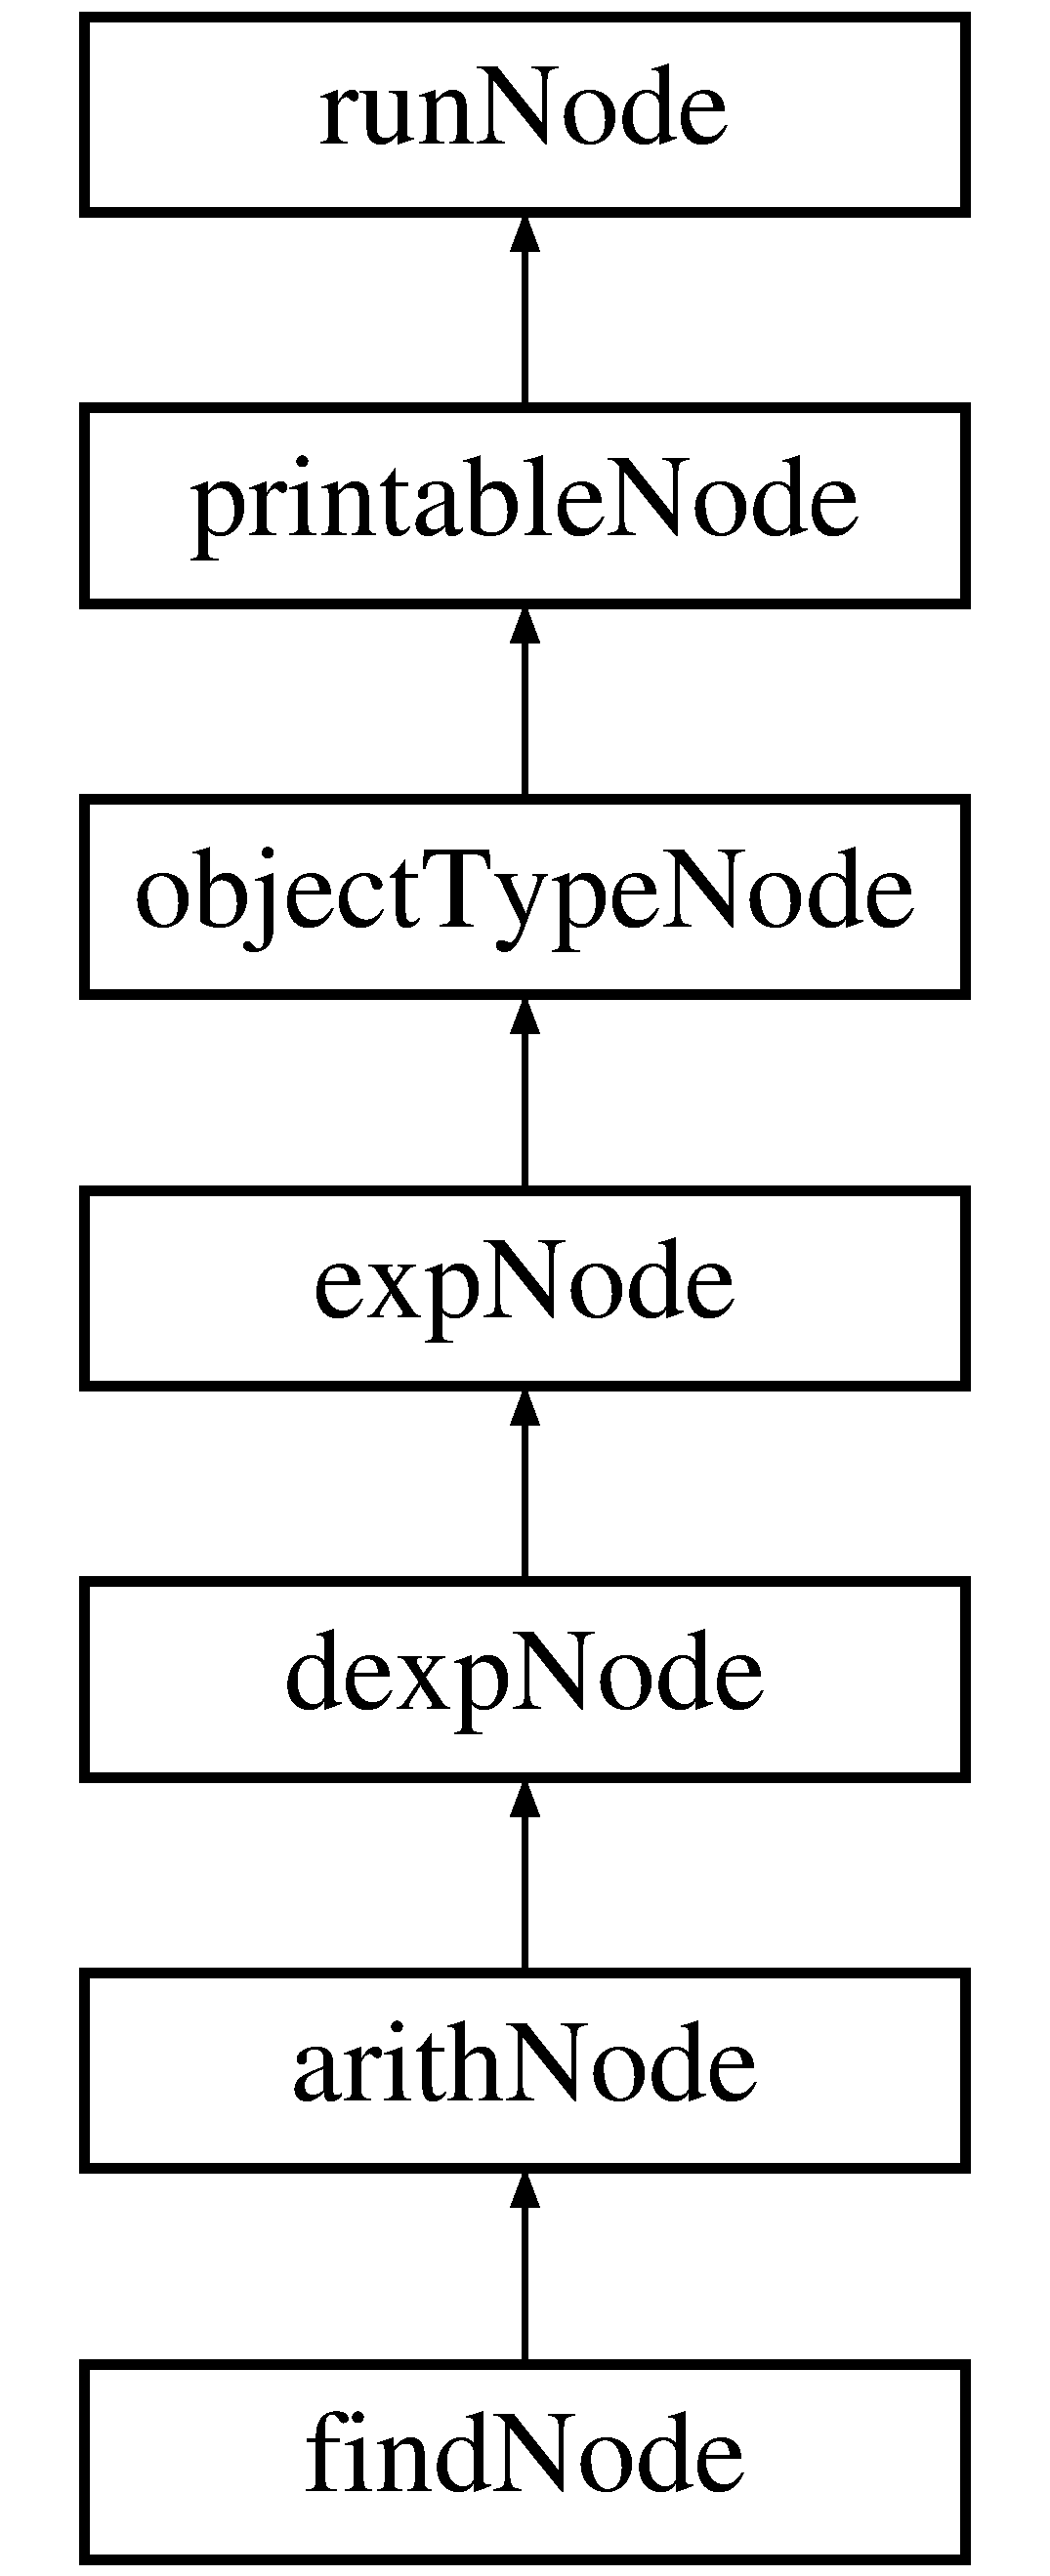
\includegraphics[height=7.000000cm]{classfindNode}
\end{center}
\end{figure}
\subsection*{Métodos públicos}
\begin{DoxyCompactItemize}
\item 
\hyperlink{classfindNode_ac09b97ca401c04472c4da0fd277bdcc9}{find\-Node} (\hyperlink{classrunNode}{run\-Node} $\ast$cad, \hyperlink{classrunNode}{run\-Node} $\ast$subcad, \hyperlink{classrunNode}{run\-Node} $\ast$ini\-\_\-pos)
\item 
void \hyperlink{classfindNode_a50ac36a34f93eb0facbd1b3c240bffc6}{run} ()
\end{DoxyCompactItemize}
\subsection*{Métodos públicos estáticos}
\begin{DoxyCompactItemize}
\item 
static \hyperlink{classrunNode}{run\-Node} $\ast$ \hyperlink{classfindNode_a6d65e85c3ee20fa14e240932dab11aa6}{as\-Method} ()
\end{DoxyCompactItemize}
\subsection*{Otros miembros heredados}


\subsection{Descripción detallada}
Nodo función búsqueda de subcadena. 

Este operador busca una subcadena de texto dentro de una cadena dada.

Para la búsqueda se precisa la cadena principal y la subcadena a buscar. Además es posible indicar a partir de qué posición se comenzará la búsqueda.

Tras la ejecución el nodo toma como valor interno el valor de la posición de la primera ocurrencia de la subcadena a partir de la posición indicada. Si la subcadena no se encuentra el nodo tomará el valor -\/1

Adicionalmente es posible utilizar como subcadena una expresión regular. 

\subsection{Documentación del constructor y destructor}
\hypertarget{classfindNode_ac09b97ca401c04472c4da0fd277bdcc9}{\index{find\-Node@{find\-Node}!find\-Node@{find\-Node}}
\index{find\-Node@{find\-Node}!findNode@{find\-Node}}
\subsubsection[{find\-Node}]{\setlength{\rightskip}{0pt plus 5cm}find\-Node\-::find\-Node (
\begin{DoxyParamCaption}
\item[{{\bf run\-Node} $\ast$}]{cad, }
\item[{{\bf run\-Node} $\ast$}]{subcad, }
\item[{{\bf run\-Node} $\ast$}]{ini\-\_\-pos}
\end{DoxyParamCaption}
)}}\label{classfindNode_ac09b97ca401c04472c4da0fd277bdcc9}
Constructor del nodo. Toma como argumentos la cadena principal la subcadena de búsqueda, que puede ser una cadena de texto o una expresión regular, y la posición a partir de la cual comenzará la búsqueda. 
\begin{DoxyParams}{Parámetros}
{\em Nodo} & cadena \\
\hline
{\em Nodo} & subcadena \\
\hline
{\em Nodo} & posición \\
\hline
\end{DoxyParams}


\subsection{Documentación de las funciones miembro}
\hypertarget{classfindNode_a6d65e85c3ee20fa14e240932dab11aa6}{\index{find\-Node@{find\-Node}!as\-Method@{as\-Method}}
\index{as\-Method@{as\-Method}!findNode@{find\-Node}}
\subsubsection[{as\-Method}]{\setlength{\rightskip}{0pt plus 5cm}{\bf run\-Node} $\ast$ find\-Node\-::as\-Method (
\begin{DoxyParamCaption}
{}
\end{DoxyParamCaption}
)\hspace{0.3cm}{\ttfamily [static]}}}\label{classfindNode_a6d65e85c3ee20fa14e240932dab11aa6}
Devuelve un nodo find como cuerpo de un nodo función, siendo un nodo this la cadena. \begin{DoxyReturn}{Devuelve}
Método find. 
\end{DoxyReturn}
\hypertarget{classfindNode_a50ac36a34f93eb0facbd1b3c240bffc6}{\index{find\-Node@{find\-Node}!run@{run}}
\index{run@{run}!findNode@{find\-Node}}
\subsubsection[{run}]{\setlength{\rightskip}{0pt plus 5cm}void find\-Node\-::run (
\begin{DoxyParamCaption}
{}
\end{DoxyParamCaption}
)\hspace{0.3cm}{\ttfamily [virtual]}}}\label{classfindNode_a50ac36a34f93eb0facbd1b3c240bffc6}
Lleva a cabo la ejecución del nodo, buscando la subcadena dentro de la cadena principal a partir de la posición indicada.

Tras la ejecución el nodo toma como valor interno la primera posición en la que se encuentra la primera ocurrencia de la subcadena.

Si la subcadena no se encuentra se tomará como valor interno el entero -\/1. 

Implementa \hyperlink{classrunNode_a83c10df8148829b08e04153c93d69eec}{run\-Node}.



La documentación para esta clase fue generada a partir de los siguientes ficheros\-:\begin{DoxyCompactItemize}
\item 
trunk/src/run/operators/\hyperlink{strOpNode_8h}{str\-Op\-Node.\-h}\item 
trunk/src/run/operators/str\-Op\-Node.\-cpp\end{DoxyCompactItemize}

\hypertarget{classfloatconvNode}{\section{Referencia de la Clase floatconv\-Node}
\label{classfloatconvNode}\index{floatconv\-Node@{floatconv\-Node}}
}


Nodo de conversión a flotante.  




{\ttfamily \#include $<$conv\-Op\-Node.\-h$>$}

Diagrama de herencias de floatconv\-Node\begin{figure}[H]
\begin{center}
\leavevmode
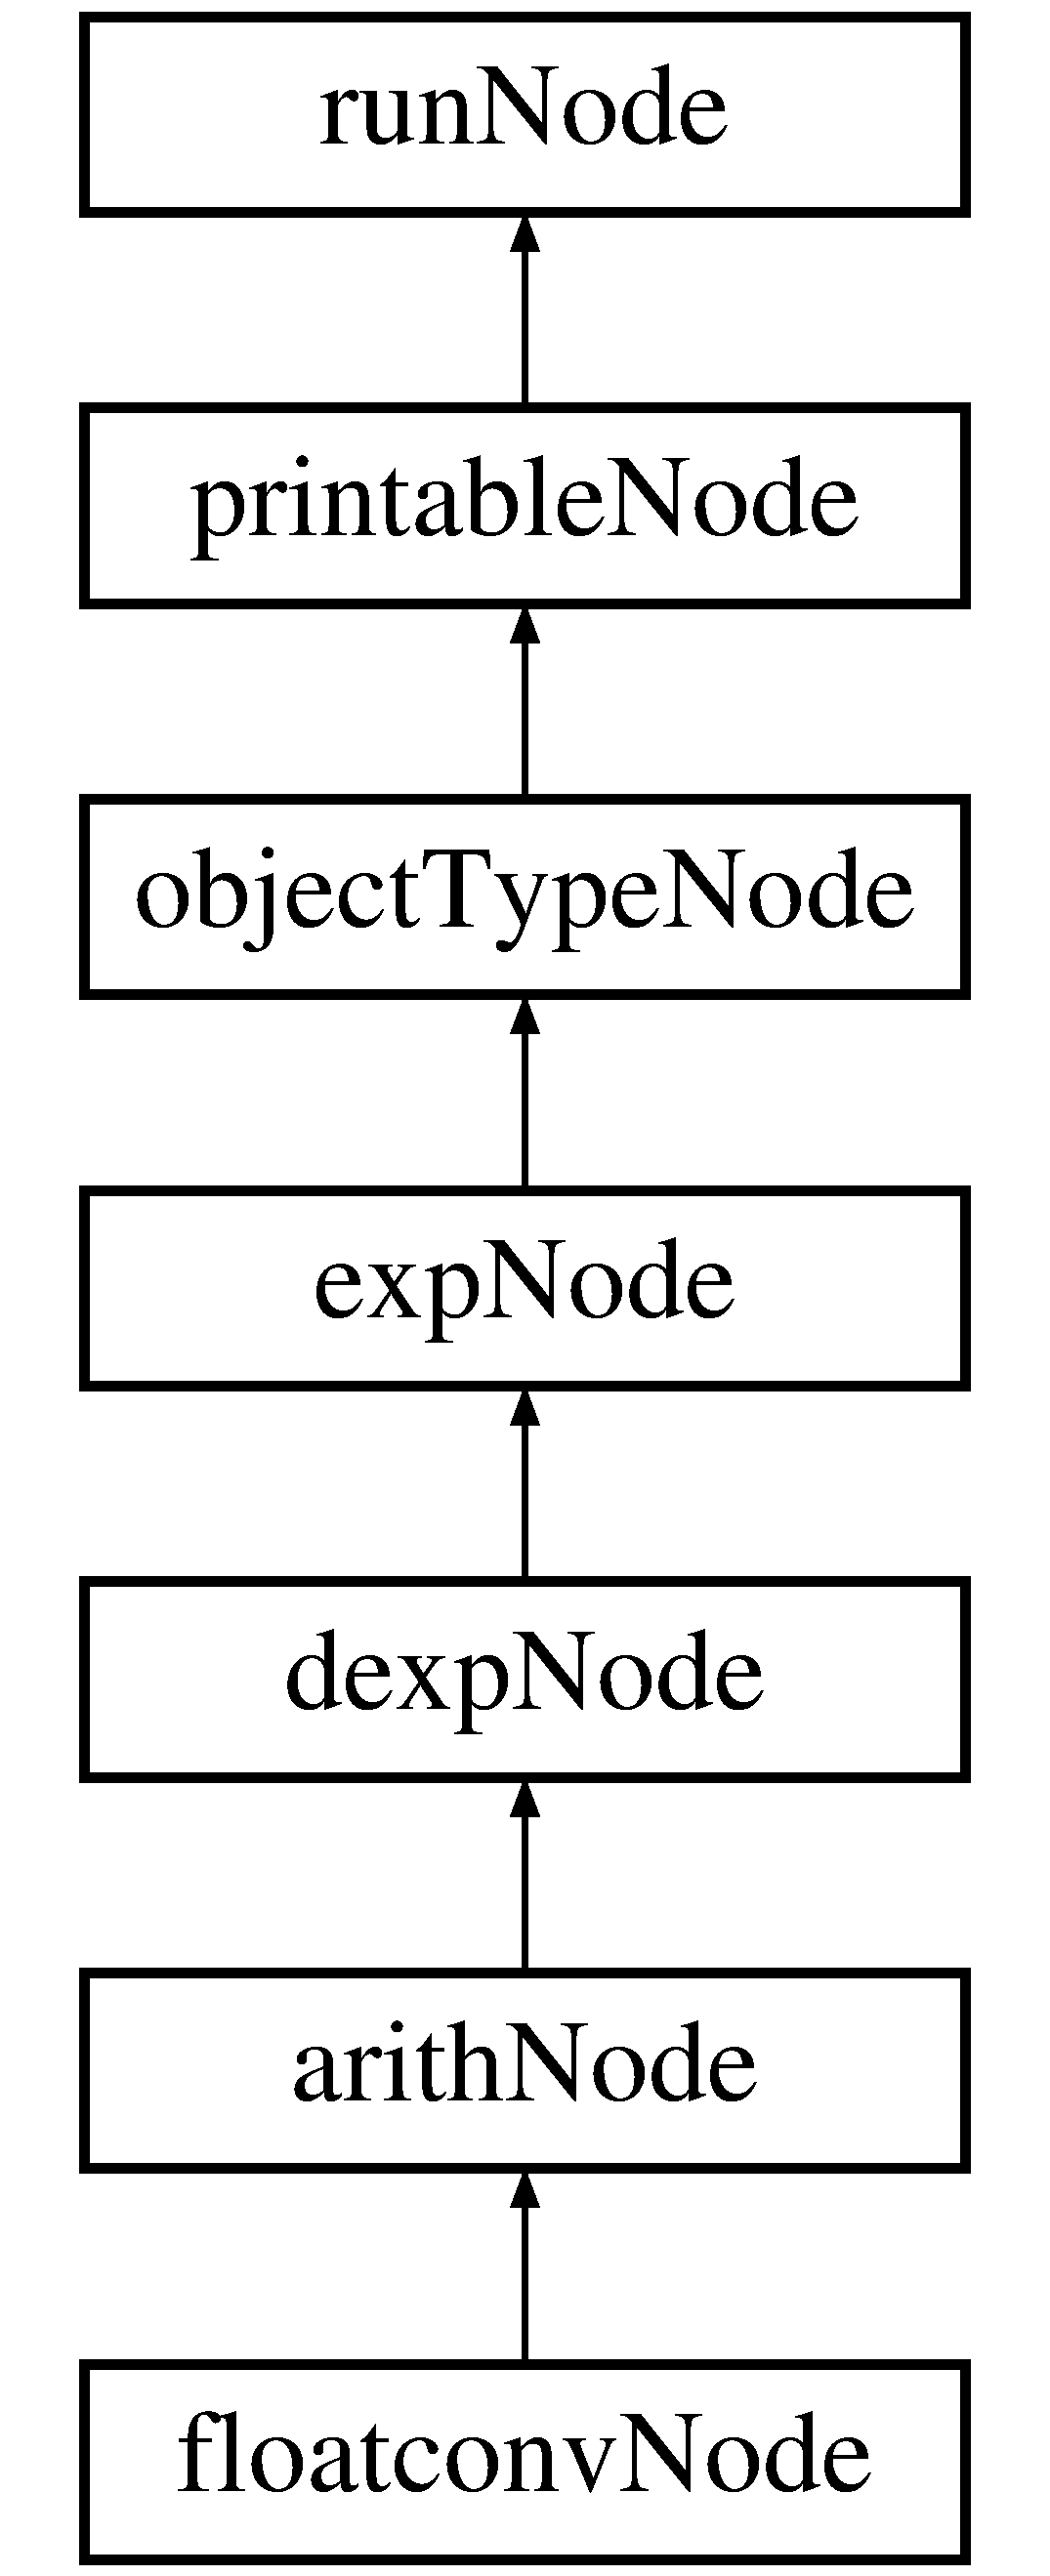
\includegraphics[height=7.000000cm]{classfloatconvNode}
\end{center}
\end{figure}
\subsection*{Métodos públicos}
\begin{DoxyCompactItemize}
\item 
\hyperlink{classfloatconvNode_a0de7468218b7634c7fabcd4bebdb3e60}{floatconv\-Node} (\hyperlink{classrunNode}{run\-Node} $\ast$node)
\item 
void \hyperlink{classfloatconvNode_ae4ffda78f5fa50df0cbf21f7eb1b1572}{run} ()
\end{DoxyCompactItemize}
\subsection*{Métodos públicos estáticos}
\begin{DoxyCompactItemize}
\item 
static num \hyperlink{classfloatconvNode_a32fa0d9657a4be471d7ca5920344fde4}{do\-\_\-floatconv} (\hyperlink{classrunNode}{run\-Node} $\ast$node)
\end{DoxyCompactItemize}
\subsection*{Otros miembros heredados}


\subsection{Descripción detallada}
Nodo de conversión a flotante. 

Este nodo fuerza la conversion a flotante del valor de un nodo

Si el nodo es booleano toma el valor de 0 ó 1 Si el nodo es aritmético toma el valor flotante del nodo Si el nodo es cadena de texto toma el valor flotante significativo de la cadena, en el caso de ser numérico. En caso contario toma el tamaño de la cadena. Si el nodo es array toma el numéro de elementos del mismo 

\subsection{Documentación del constructor y destructor}
\hypertarget{classfloatconvNode_a0de7468218b7634c7fabcd4bebdb3e60}{\index{floatconv\-Node@{floatconv\-Node}!floatconv\-Node@{floatconv\-Node}}
\index{floatconv\-Node@{floatconv\-Node}!floatconvNode@{floatconv\-Node}}
\subsubsection[{floatconv\-Node}]{\setlength{\rightskip}{0pt plus 5cm}floatconv\-Node\-::floatconv\-Node (
\begin{DoxyParamCaption}
\item[{{\bf run\-Node} $\ast$}]{node}
\end{DoxyParamCaption}
)}}\label{classfloatconvNode_a0de7468218b7634c7fabcd4bebdb3e60}
Constructor de la clase. Asocia el nodo operador a un nodo. 
\begin{DoxyParams}{Parámetros}
{\em node} & Nodo operando. \\
\hline
\end{DoxyParams}


\subsection{Documentación de las funciones miembro}
\hypertarget{classfloatconvNode_a32fa0d9657a4be471d7ca5920344fde4}{\index{floatconv\-Node@{floatconv\-Node}!do\-\_\-floatconv@{do\-\_\-floatconv}}
\index{do\-\_\-floatconv@{do\-\_\-floatconv}!floatconvNode@{floatconv\-Node}}
\subsubsection[{do\-\_\-floatconv}]{\setlength{\rightskip}{0pt plus 5cm}num floatconv\-Node\-::do\-\_\-floatconv (
\begin{DoxyParamCaption}
\item[{{\bf run\-Node} $\ast$}]{node}
\end{DoxyParamCaption}
)\hspace{0.3cm}{\ttfamily [static]}}}\label{classfloatconvNode_a32fa0d9657a4be471d7ca5920344fde4}
Convierte un nodo a su valor flotante 
\begin{DoxyParams}{Parámetros}
{\em node} & Nodo operando. \\
\hline
\end{DoxyParams}
\begin{DoxyReturn}{Devuelve}
Valor de la operación 
\end{DoxyReturn}
\hypertarget{classfloatconvNode_ae4ffda78f5fa50df0cbf21f7eb1b1572}{\index{floatconv\-Node@{floatconv\-Node}!run@{run}}
\index{run@{run}!floatconvNode@{floatconv\-Node}}
\subsubsection[{run}]{\setlength{\rightskip}{0pt plus 5cm}void floatconv\-Node\-::run (
\begin{DoxyParamCaption}
{}
\end{DoxyParamCaption}
)\hspace{0.3cm}{\ttfamily [virtual]}}}\label{classfloatconvNode_ae4ffda78f5fa50df0cbf21f7eb1b1572}
Tras ser ejecutado el operador toma como valor el resultado de la conversión a flotante del nodo asociado 

Implementa \hyperlink{classrunNode_a83c10df8148829b08e04153c93d69eec}{run\-Node}.



La documentación para esta clase fue generada a partir de los siguientes ficheros\-:\begin{DoxyCompactItemize}
\item 
trunk/src/run/operators/\hyperlink{convOpNode_8h}{conv\-Op\-Node.\-h}\item 
trunk/src/run/operators/conv\-Op\-Node.\-cpp\end{DoxyCompactItemize}

\hypertarget{classforeachGeneratorNode}{\section{Referencia de la Clase foreach\-Generator\-Node}
\label{classforeachGeneratorNode}\index{foreach\-Generator\-Node@{foreach\-Generator\-Node}}
}


Nodo para la lista por compresión.  




{\ttfamily \#include $<$loop\-Stmt\-Node.\-h$>$}

Diagrama de herencias de foreach\-Generator\-Node\begin{figure}[H]
\begin{center}
\leavevmode
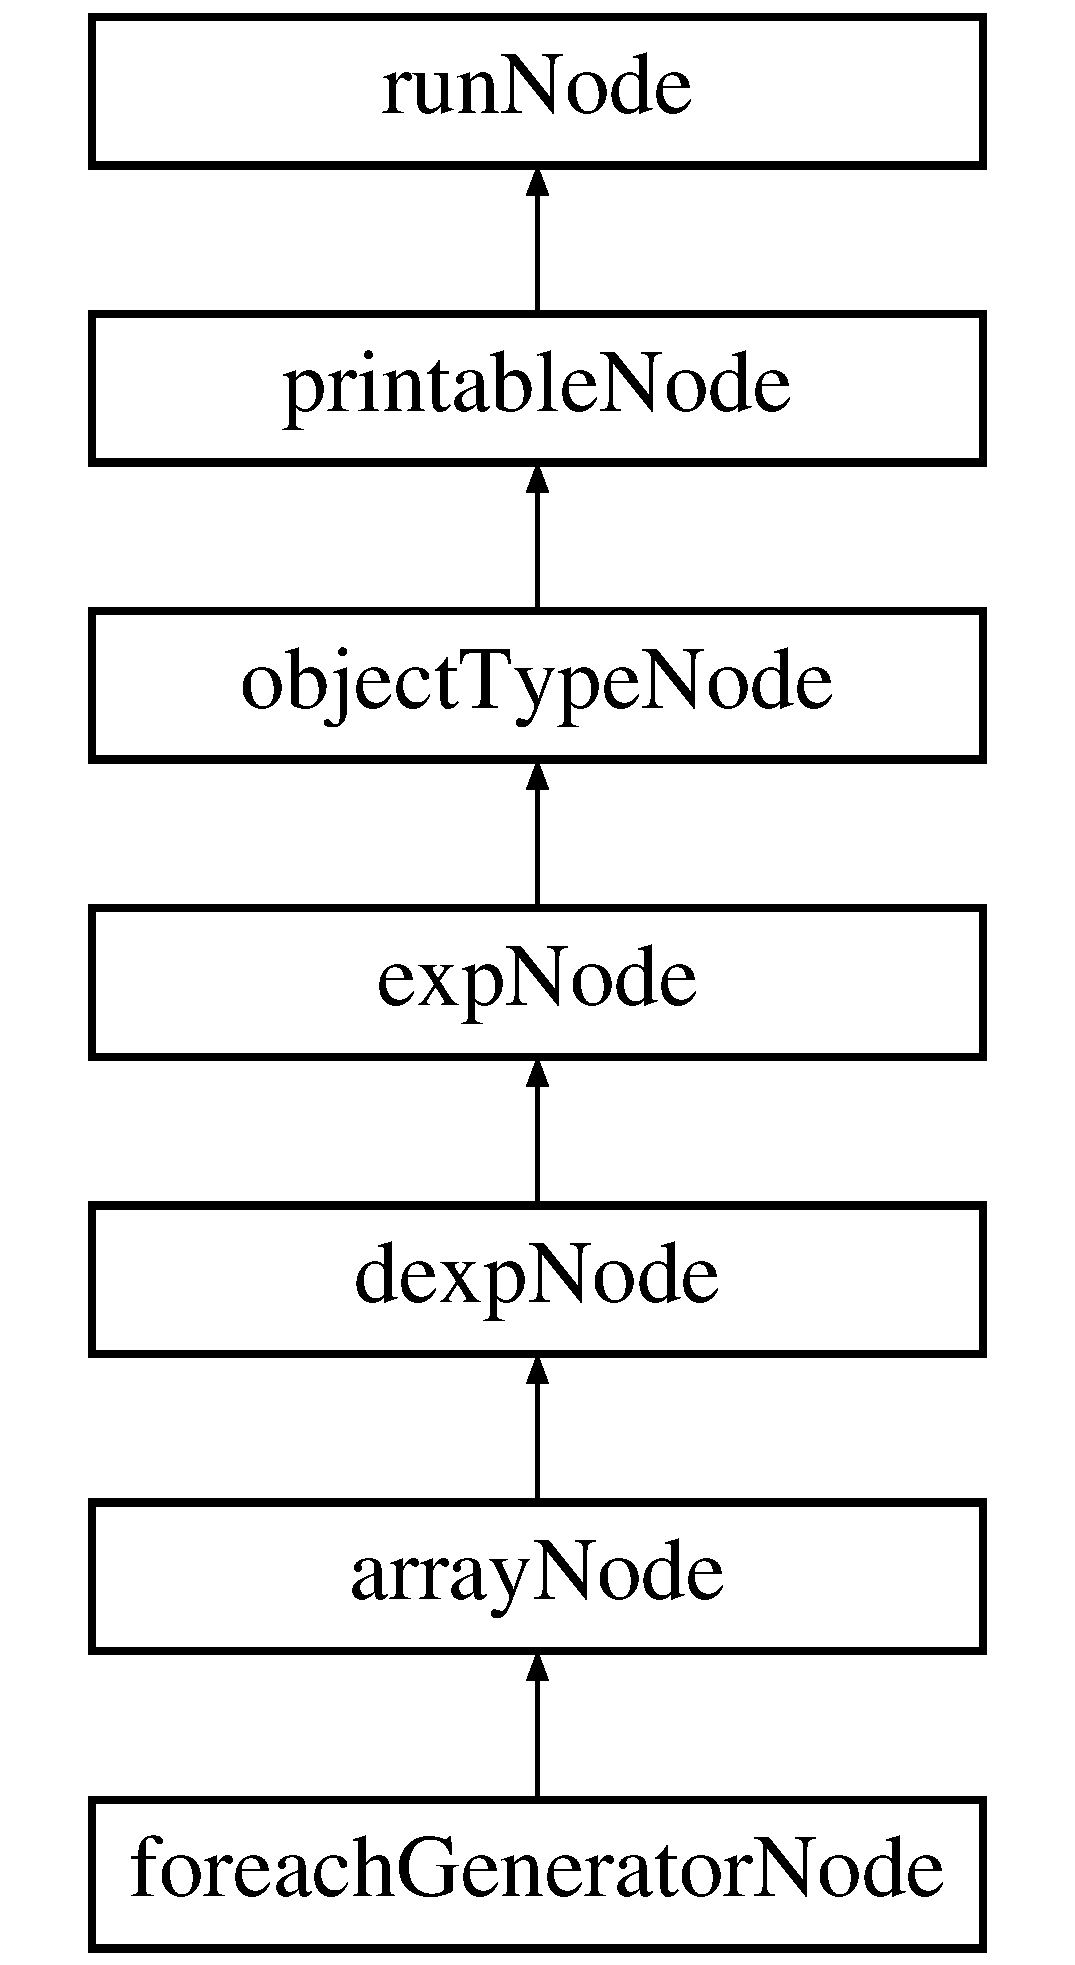
\includegraphics[height=7.000000cm]{classforeachGeneratorNode}
\end{center}
\end{figure}
\subsection*{Métodos públicos}
\begin{DoxyCompactItemize}
\item 
\hyperlink{classforeachGeneratorNode_af80083b17f10891c36164b3a07118736}{foreach\-Generator\-Node} (\hyperlink{classrunNode}{run\-Node} $\ast$elem, \hyperlink{classrunNode}{run\-Node} $\ast$val, \hyperlink{classrunNode}{run\-Node} $\ast$exp, \hyperlink{classrunNode}{run\-Node} $\ast$rb, \hyperlink{classrunNode}{run\-Node} $\ast$key=N\-U\-L\-L, \hyperlink{classrunNode}{run\-Node} $\ast$if\-\_\-cond=N\-U\-L\-L, \hyperlink{classrunNode}{run\-Node} $\ast$elem\-\_\-key=N\-U\-L\-L)
\item 
void \hyperlink{classforeachGeneratorNode_a2769b5956850366b99fa9f9d0e89ec37}{run} ()
\end{DoxyCompactItemize}
\subsection*{Otros miembros heredados}


\subsection{Descripción detallada}
Nodo para la lista por compresión. 

Representa una expresión cuyo valor es obtenido a partir de una sentencia iterativa.

La forma más simple de crear una lista por compresión es mediante una expresión de generación y una variable que iterará sobre una expresión conjunto. En cada iteración la variable iteradora tomará un valor del conjunto. Para cada elemento se calculará el valor de la expresión generadora, la cual normalmente contendrá la variable iteradora, y será introducido en un array que será tomado como valor.

El conjunto sobre el que se itera dependerá del tipo de dato obtenido al evaluar la expresión conjunto\-:
\begin{DoxyItemize}
\item Booleano\-: Se itera hasta que se evalúa como falso. En cada iteración se asigna el entero correspondiente al número de la misma.
\item Numérico\-: Si es positivo se itera desde cero hasta el valor sin incluirlo. Si es negativo no se itera.
\item Cadena de caracteres\-: Se itera por cada carácter en la cadena.
\item Array\-: Se itera por cada elemento en el array.
\end{DoxyItemize}

Es posible filtrar los datos que serán incluidos en el array, añadiendo una condición que se deba cumplir.

También se puede especificar una identificador que guarde la clave de la referencia del elemento iterado.

El array resultado puede ser generado mediante la expresión de generación y otra expresión que se corresponda con la clave del elemento creado.

Antes de generar el elemento del array que se tomará como valor es posible ejecutar un bloque de sentencias. 

\subsection{Documentación del constructor y destructor}
\hypertarget{classforeachGeneratorNode_af80083b17f10891c36164b3a07118736}{\index{foreach\-Generator\-Node@{foreach\-Generator\-Node}!foreach\-Generator\-Node@{foreach\-Generator\-Node}}
\index{foreach\-Generator\-Node@{foreach\-Generator\-Node}!foreachGeneratorNode@{foreach\-Generator\-Node}}
\subsubsection[{foreach\-Generator\-Node}]{\setlength{\rightskip}{0pt plus 5cm}foreach\-Generator\-Node\-::foreach\-Generator\-Node (
\begin{DoxyParamCaption}
\item[{{\bf run\-Node} $\ast$}]{elem, }
\item[{{\bf run\-Node} $\ast$}]{val, }
\item[{{\bf run\-Node} $\ast$}]{exp, }
\item[{{\bf run\-Node} $\ast$}]{rb, }
\item[{{\bf run\-Node} $\ast$}]{key = {\ttfamily NULL}, }
\item[{{\bf run\-Node} $\ast$}]{if\-\_\-cond = {\ttfamily NULL}, }
\item[{{\bf run\-Node} $\ast$}]{elem\-\_\-key = {\ttfamily NULL}}
\end{DoxyParamCaption}
)}}\label{classforeachGeneratorNode_af80083b17f10891c36164b3a07118736}
Constructor de la clase. 
\begin{DoxyParams}{Parámetros}
{\em elem} & Nodo que representa el conjunto de elementos. \\
\hline
{\em val} & Nodo que hace de identificador para el valor de cada iteración. \\
\hline
{\em exp} & Nodo que hace de expresión generadora. \\
\hline
{\em rb} & Nodo que representa el bloque de sentencias que será ejecutada en cada iteración. \\
\hline
{\em key} & Nodo que hace de identificador para la clave de cada itereación. \\
\hline
{\em if\-\_\-cond} & Nodo que hace de condición para que se lleve a cabo la insercción de los elementos de la iteración. \\
\hline
{\em elem\-\_\-key} & Nodo que representa la expresión generadora de la clave del elemento en la iteración. \\
\hline
\end{DoxyParams}


\subsection{Documentación de las funciones miembro}
\hypertarget{classforeachGeneratorNode_a2769b5956850366b99fa9f9d0e89ec37}{\index{foreach\-Generator\-Node@{foreach\-Generator\-Node}!run@{run}}
\index{run@{run}!foreachGeneratorNode@{foreach\-Generator\-Node}}
\subsubsection[{run}]{\setlength{\rightskip}{0pt plus 5cm}void foreach\-Generator\-Node\-::run (
\begin{DoxyParamCaption}
{}
\end{DoxyParamCaption}
)\hspace{0.3cm}{\ttfamily [virtual]}}}\label{classforeachGeneratorNode_a2769b5956850366b99fa9f9d0e89ec37}
Método que lleva a cabo la ejecución del modo. Toma como valor el array generado de forma iterativa. 

Implementa \hyperlink{classrunNode_a83c10df8148829b08e04153c93d69eec}{run\-Node}.



La documentación para esta clase fue generada a partir de los siguientes ficheros\-:\begin{DoxyCompactItemize}
\item 
trunk/src/run/stmts/\hyperlink{loopStmtNode_8h}{loop\-Stmt\-Node.\-h}\item 
trunk/src/run/stmts/loop\-Stmt\-Node.\-cpp\end{DoxyCompactItemize}

\hypertarget{classforeachNode}{\section{Referencia de la Clase foreach\-Node}
\label{classforeachNode}\index{foreach\-Node@{foreach\-Node}}
}


Nodo sentencia foreach.  




{\ttfamily \#include $<$loop\-Stmt\-Node.\-h$>$}

Diagrama de herencias de foreach\-Node\begin{figure}[H]
\begin{center}
\leavevmode
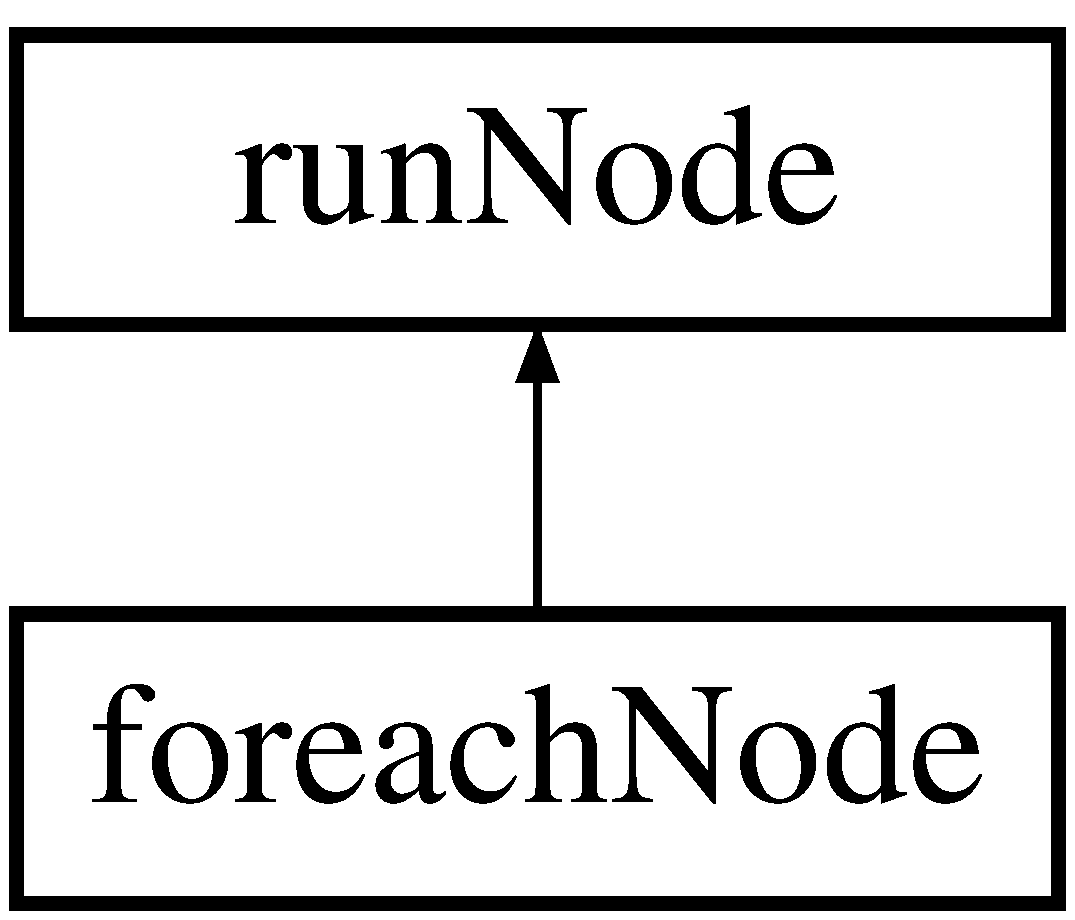
\includegraphics[height=2.000000cm]{classforeachNode}
\end{center}
\end{figure}
\subsection*{Métodos públicos}
\begin{DoxyCompactItemize}
\item 
\hyperlink{classforeachNode_aa30f6b951da73f3637be795670a807f3}{foreach\-Node} (\hyperlink{classrunNode}{run\-Node} $\ast$val, \hyperlink{classrunNode}{run\-Node} $\ast$exp, \hyperlink{classrunNode}{run\-Node} $\ast$rb=N\-U\-L\-L, \hyperlink{classrunNode}{run\-Node} $\ast$key=N\-U\-L\-L)
\item 
void \hyperlink{classforeachNode_a86c6a9ef828c2a700a29d725a0bc4a53}{run} ()
\end{DoxyCompactItemize}
\subsection*{Otros miembros heredados}


\subsection{Descripción detallada}
Nodo sentencia foreach. 

Este nodo representa una sentencia foreach. Permite ejecutar un bloque de sentencias para cada elemento contenido en un conjunto.

Se construye a partir un nodo que hace de conjunto a recorrer, un nodo que hace de identificador, el cual referenciará al elemento actual en cada iteración y un nodo que hace de bloque de sentencias que se ejecutará para cada elemento. Es posible además especificar un nodo que hará de identificador en el que se guardará las claves de las referencias a los elementos recorridos. 

\subsection{Documentación del constructor y destructor}
\hypertarget{classforeachNode_aa30f6b951da73f3637be795670a807f3}{\index{foreach\-Node@{foreach\-Node}!foreach\-Node@{foreach\-Node}}
\index{foreach\-Node@{foreach\-Node}!foreachNode@{foreach\-Node}}
\subsubsection[{foreach\-Node}]{\setlength{\rightskip}{0pt plus 5cm}foreach\-Node\-::foreach\-Node (
\begin{DoxyParamCaption}
\item[{{\bf run\-Node} $\ast$}]{val, }
\item[{{\bf run\-Node} $\ast$}]{exp, }
\item[{{\bf run\-Node} $\ast$}]{rb = {\ttfamily NULL}, }
\item[{{\bf run\-Node} $\ast$}]{key = {\ttfamily NULL}}
\end{DoxyParamCaption}
)}}\label{classforeachNode_aa30f6b951da73f3637be795670a807f3}
Constructor de la clase. 
\begin{DoxyParams}{Parámetros}
{\em val} & Nodo que hace de identificador para el valor de cada iteración. \\
\hline
{\em exp} & Nodo que hace de conjunto de elementos. \\
\hline
{\em rb} & Nodo que hace de bloque de sentencias. \\
\hline
{\em key} & Nodo que hace de identificador para la clave de cada iteración. \\
\hline
\end{DoxyParams}


\subsection{Documentación de las funciones miembro}
\hypertarget{classforeachNode_a86c6a9ef828c2a700a29d725a0bc4a53}{\index{foreach\-Node@{foreach\-Node}!run@{run}}
\index{run@{run}!foreachNode@{foreach\-Node}}
\subsubsection[{run}]{\setlength{\rightskip}{0pt plus 5cm}void foreach\-Node\-::run (
\begin{DoxyParamCaption}
{}
\end{DoxyParamCaption}
)\hspace{0.3cm}{\ttfamily [virtual]}}}\label{classforeachNode_a86c6a9ef828c2a700a29d725a0bc4a53}
Método de ejecución del nodo. Ejecuta el bloque de sentencias para cada elemento contenido en el conjunto, asignado el elemento al identificador del valor y la clave al identificador de clave si se facilitó. 

Implementa \hyperlink{classrunNode_a83c10df8148829b08e04153c93d69eec}{run\-Node}.



La documentación para esta clase fue generada a partir de los siguientes ficheros\-:\begin{DoxyCompactItemize}
\item 
trunk/src/run/stmts/\hyperlink{loopStmtNode_8h}{loop\-Stmt\-Node.\-h}\item 
trunk/src/run/stmts/loop\-Stmt\-Node.\-cpp\end{DoxyCompactItemize}

\hypertarget{classforkNode}{\section{Referencia de la Clase fork\-Node}
\label{classforkNode}\index{fork\-Node@{fork\-Node}}
}


Nodo función fork.  




{\ttfamily \#include $<$process\-Op\-Node.\-h$>$}

Diagrama de herencias de fork\-Node\begin{figure}[H]
\begin{center}
\leavevmode
\includegraphics[height=7.000000cm]{classforkNode}
\end{center}
\end{figure}
\subsection*{Métodos públicos}
\begin{DoxyCompactItemize}
\item 
\hyperlink{classforkNode_a0136ac241984f4ba15322837976f8baf}{fork\-Node} ()
\item 
void \hyperlink{classforkNode_a7b3213a5ad54b2d051f9b1a96b88d5fd}{run} ()
\end{DoxyCompactItemize}
\subsection*{Otros miembros heredados}


\subsection{Descripción detallada}
Nodo función fork. 

El nodo fork crea una bifurcación en el proceso actual. Cuando este nodo es ejecutado se crea un proceso (hijo) copia del proceso actual (padre). En el proceso hijo el nodo tomará como valor aritmético 0, mientras que en el proceso padre tomará como valor el identificador de proceso del hijo. 

\subsection{Documentación del constructor y destructor}
\hypertarget{classforkNode_a0136ac241984f4ba15322837976f8baf}{\index{fork\-Node@{fork\-Node}!fork\-Node@{fork\-Node}}
\index{fork\-Node@{fork\-Node}!forkNode@{fork\-Node}}
\subsubsection[{fork\-Node}]{\setlength{\rightskip}{0pt plus 5cm}fork\-Node\-::fork\-Node (
\begin{DoxyParamCaption}
{}
\end{DoxyParamCaption}
)}}\label{classforkNode_a0136ac241984f4ba15322837976f8baf}
Constructor de la clase. 

\subsection{Documentación de las funciones miembro}
\hypertarget{classforkNode_a7b3213a5ad54b2d051f9b1a96b88d5fd}{\index{fork\-Node@{fork\-Node}!run@{run}}
\index{run@{run}!forkNode@{fork\-Node}}
\subsubsection[{run}]{\setlength{\rightskip}{0pt plus 5cm}void fork\-Node\-::run (
\begin{DoxyParamCaption}
{}
\end{DoxyParamCaption}
)\hspace{0.3cm}{\ttfamily [virtual]}}}\label{classforkNode_a7b3213a5ad54b2d051f9b1a96b88d5fd}
Metodo de ejecución. Crea una bifurcación en el proceso actual. Cuando este nodo es ejecutado se crea un proceso (hijo) copia del proceso actual (padre). En el proceso hijo el nodo tomará como valor aritmético 0, mientras que en el proceso padre tomará como valor el identificador de proceso del hijo. 

Implementa \hyperlink{classrunNode_a83c10df8148829b08e04153c93d69eec}{run\-Node}.



La documentación para esta clase fue generada a partir de los siguientes ficheros\-:\begin{DoxyCompactItemize}
\item 
trunk/src/run/operators/\hyperlink{processOpNode_8h}{process\-Op\-Node.\-h}\item 
trunk/src/run/operators/process\-Op\-Node.\-cpp\end{DoxyCompactItemize}

\hypertarget{classforNode}{\section{Referencia de la Clase for\-Node}
\label{classforNode}\index{for\-Node@{for\-Node}}
}


Nodo sentencia iterativa for.  




{\ttfamily \#include $<$loop\-Stmt\-Node.\-h$>$}

Diagrama de herencias de for\-Node\begin{figure}[H]
\begin{center}
\leavevmode
\includegraphics[height=2.000000cm]{classforNode}
\end{center}
\end{figure}
\subsection*{Métodos públicos}
\begin{DoxyCompactItemize}
\item 
\hyperlink{classforNode_a1a300d8edd6016fe323b3bf4ec2f34fc}{for\-Node} (\hyperlink{classrunNode}{run\-Node} $\ast$asig, \hyperlink{classrunNode}{run\-Node} $\ast$exp, \hyperlink{classrunNode}{run\-Node} $\ast$inc, \hyperlink{classrunNode}{run\-Node} $\ast$rb)
\item 
void \hyperlink{classforNode_aaec3e2c55e856503df16c17c1ae1f254}{run} ()
\end{DoxyCompactItemize}
\subsection*{Otros miembros heredados}


\subsection{Descripción detallada}
Nodo sentencia iterativa for. 

Este nodo consta de una expresión de asignación, una condición, una expresión de incremento y un bloque de sentencias. Se ejecuta la expresión de asignación, luego mientras se cumpla la condición se ejecuta el bloque de sentencias y la expresión de incremento. 

\subsection{Documentación del constructor y destructor}
\hypertarget{classforNode_a1a300d8edd6016fe323b3bf4ec2f34fc}{\index{for\-Node@{for\-Node}!for\-Node@{for\-Node}}
\index{for\-Node@{for\-Node}!forNode@{for\-Node}}
\subsubsection[{for\-Node}]{\setlength{\rightskip}{0pt plus 5cm}for\-Node\-::for\-Node (
\begin{DoxyParamCaption}
\item[{{\bf run\-Node} $\ast$}]{asig, }
\item[{{\bf run\-Node} $\ast$}]{exp, }
\item[{{\bf run\-Node} $\ast$}]{inc, }
\item[{{\bf run\-Node} $\ast$}]{rb}
\end{DoxyParamCaption}
)}}\label{classforNode_a1a300d8edd6016fe323b3bf4ec2f34fc}
Constructor de la clase. 
\begin{DoxyParams}{Parámetros}
{\em asig} & Nodo que representa la expresión de asignación. \\
\hline
{\em exp} & Nodo que representa la expresión de condición. \\
\hline
{\em inc} & Nodo que representa la expresión de incremento. \\
\hline
{\em rb} & Nodo que representa el bloque de sentencias. \\
\hline
\end{DoxyParams}


\subsection{Documentación de las funciones miembro}
\hypertarget{classforNode_aaec3e2c55e856503df16c17c1ae1f254}{\index{for\-Node@{for\-Node}!run@{run}}
\index{run@{run}!forNode@{for\-Node}}
\subsubsection[{run}]{\setlength{\rightskip}{0pt plus 5cm}void for\-Node\-::run (
\begin{DoxyParamCaption}
{}
\end{DoxyParamCaption}
)\hspace{0.3cm}{\ttfamily [virtual]}}}\label{classforNode_aaec3e2c55e856503df16c17c1ae1f254}
Método que ejecuta el nodo. Ejecuta el nodo que hace de la expresión de asignación. Luego ejecuta y evalua la condición. Si se da un resultado verdadero se ejecuta el bloque de sentencias y la expresión de incremento. Entonces la condición se vuelve a evaluar repitiéndose el proceso desde este punto hasta que es evaluada como falsa. 

Implementa \hyperlink{classrunNode_a83c10df8148829b08e04153c93d69eec}{run\-Node}.



La documentación para esta clase fue generada a partir de los siguientes ficheros\-:\begin{DoxyCompactItemize}
\item 
trunk/src/run/stmts/\hyperlink{loopStmtNode_8h}{loop\-Stmt\-Node.\-h}\item 
trunk/src/run/stmts/loop\-Stmt\-Node.\-cpp\end{DoxyCompactItemize}

\hypertarget{classfputNode}{\section{Referencia de la Clase fput\-Node}
\label{classfputNode}\index{fput\-Node@{fput\-Node}}
}


Node función escribir en descriptor de fichero .  




{\ttfamily \#include $<$file\-Op\-Node.\-h$>$}

Diagrama de herencias de fput\-Node\begin{figure}[H]
\begin{center}
\leavevmode
\includegraphics[height=7.000000cm]{classfputNode}
\end{center}
\end{figure}
\subsection*{Métodos públicos}
\begin{DoxyCompactItemize}
\item 
\hyperlink{classfputNode_a86bc8a68a443cf689a4631d4aaddb8a8}{fput\-Node} (\hyperlink{classrunNode}{run\-Node} $\ast$file, \hyperlink{classrunNode}{run\-Node} $\ast$val)
\item 
void \hyperlink{classfputNode_ac1e5fdc58f9d57e1b7782b1eda9e273f}{run} ()
\end{DoxyCompactItemize}
\subsection*{Otros miembros heredados}


\subsection{Descripción detallada}
Node función escribir en descriptor de fichero . 

Este nodo se encarga escribir en la posición en la que se encuentra un descriptor de fichero una cadena. 

\subsection{Documentación del constructor y destructor}
\hypertarget{classfputNode_a86bc8a68a443cf689a4631d4aaddb8a8}{\index{fput\-Node@{fput\-Node}!fput\-Node@{fput\-Node}}
\index{fput\-Node@{fput\-Node}!fputNode@{fput\-Node}}
\subsubsection[{fput\-Node}]{\setlength{\rightskip}{0pt plus 5cm}fput\-Node\-::fput\-Node (
\begin{DoxyParamCaption}
\item[{{\bf run\-Node} $\ast$}]{file, }
\item[{{\bf run\-Node} $\ast$}]{val}
\end{DoxyParamCaption}
)}}\label{classfputNode_a86bc8a68a443cf689a4631d4aaddb8a8}
Constructor de la clase. 
\begin{DoxyParams}{Parámetros}
{\em file.} & Nodo que reresenta el descriptor de fichero \\
\hline
{\em val.} & Nodo que representa la cadena a escribir \\
\hline
\end{DoxyParams}


\subsection{Documentación de las funciones miembro}
\hypertarget{classfputNode_ac1e5fdc58f9d57e1b7782b1eda9e273f}{\index{fput\-Node@{fput\-Node}!run@{run}}
\index{run@{run}!fputNode@{fput\-Node}}
\subsubsection[{run}]{\setlength{\rightskip}{0pt plus 5cm}void fput\-Node\-::run (
\begin{DoxyParamCaption}
{}
\end{DoxyParamCaption}
)\hspace{0.3cm}{\ttfamily [virtual]}}}\label{classfputNode_ac1e5fdc58f9d57e1b7782b1eda9e273f}
Método de ejecución. Escribe en la posición en la que se enncuentra el descriptor de fichero la cadena dada.

Toma como valor el número de caracteres escritos. 

Implementa \hyperlink{classrunNode_a83c10df8148829b08e04153c93d69eec}{run\-Node}.



La documentación para esta clase fue generada a partir de los siguientes ficheros\-:\begin{DoxyCompactItemize}
\item 
trunk/src/run/operators/\hyperlink{fileOpNode_8h}{file\-Op\-Node.\-h}\item 
trunk/src/run/operators/file\-Op\-Node.\-cpp\end{DoxyCompactItemize}

\hypertarget{classfreadNode}{\section{Referencia de la Clase fread\-Node}
\label{classfreadNode}\index{fread\-Node@{fread\-Node}}
}


Node función leer fichero.  




{\ttfamily \#include $<$file\-Op\-Node.\-h$>$}

Diagrama de herencias de fread\-Node\begin{figure}[H]
\begin{center}
\leavevmode
\includegraphics[height=7.000000cm]{classfreadNode}
\end{center}
\end{figure}
\subsection*{Métodos públicos}
\begin{DoxyCompactItemize}
\item 
\hyperlink{classfreadNode_aebdab762c8e7a5834a6365035a3ca00d}{fread\-Node} (\hyperlink{classrunNode}{run\-Node} $\ast$file)
\item 
void \hyperlink{classfreadNode_a70bf100a17d78be82f7972d467b22fe8}{run} ()
\end{DoxyCompactItemize}
\subsection*{Otros miembros heredados}


\subsection{Descripción detallada}
Node función leer fichero. 

Este nodo se encarga de leer todo el contenido de un fichero y tomar la cadena correspondiente como valor. 

\subsection{Documentación del constructor y destructor}
\hypertarget{classfreadNode_aebdab762c8e7a5834a6365035a3ca00d}{\index{fread\-Node@{fread\-Node}!fread\-Node@{fread\-Node}}
\index{fread\-Node@{fread\-Node}!freadNode@{fread\-Node}}
\subsubsection[{fread\-Node}]{\setlength{\rightskip}{0pt plus 5cm}fread\-Node\-::fread\-Node (
\begin{DoxyParamCaption}
\item[{{\bf run\-Node} $\ast$}]{file}
\end{DoxyParamCaption}
)}}\label{classfreadNode_aebdab762c8e7a5834a6365035a3ca00d}
Constructor de la clase. 
\begin{DoxyParams}{Parámetros}
{\em file.} & Nodo que representa la ruta del fichero a leer. \\
\hline
\end{DoxyParams}


\subsection{Documentación de las funciones miembro}
\hypertarget{classfreadNode_a70bf100a17d78be82f7972d467b22fe8}{\index{fread\-Node@{fread\-Node}!run@{run}}
\index{run@{run}!freadNode@{fread\-Node}}
\subsubsection[{run}]{\setlength{\rightskip}{0pt plus 5cm}void fread\-Node\-::run (
\begin{DoxyParamCaption}
{}
\end{DoxyParamCaption}
)\hspace{0.3cm}{\ttfamily [virtual]}}}\label{classfreadNode_a70bf100a17d78be82f7972d467b22fe8}
Método de ejecución. Procede a la lectura del fichero y toma como valor la cadena resultante. Si el fichero no existe se produce un error. 

Implementa \hyperlink{classrunNode_a83c10df8148829b08e04153c93d69eec}{run\-Node}.



La documentación para esta clase fue generada a partir de los siguientes ficheros\-:\begin{DoxyCompactItemize}
\item 
trunk/src/run/operators/\hyperlink{fileOpNode_8h}{file\-Op\-Node.\-h}\item 
trunk/src/run/operators/file\-Op\-Node.\-cpp\end{DoxyCompactItemize}

\hypertarget{classfseekNode}{\section{Referencia de la Clase fseek\-Node}
\label{classfseekNode}\index{fseek\-Node@{fseek\-Node}}
}


Nodo función cambiar puntero de descriptor de fichero.  




{\ttfamily \#include $<$file\-Op\-Node.\-h$>$}

Diagrama de herencias de fseek\-Node\begin{figure}[H]
\begin{center}
\leavevmode
\includegraphics[height=7.000000cm]{classfseekNode}
\end{center}
\end{figure}
\subsection*{Métodos públicos}
\begin{DoxyCompactItemize}
\item 
\hyperlink{classfseekNode_a15a163ad45fe50710ce3a9b2c7032160}{fseek\-Node} (\hyperlink{classrunNode}{run\-Node} $\ast$file, \hyperlink{classrunNode}{run\-Node} $\ast$offset, int pos=0)
\item 
void \hyperlink{classfseekNode_aec2f6985f9df3761c36d063d7d32b59c}{run} ()
\end{DoxyCompactItemize}
\subsection*{Otros miembros heredados}


\subsection{Descripción detallada}
Nodo función cambiar puntero de descriptor de fichero. 

Este nodo se encarga de cambiar la posición del puntero que representa el descriptor a un fichero. 

\subsection{Documentación del constructor y destructor}
\hypertarget{classfseekNode_a15a163ad45fe50710ce3a9b2c7032160}{\index{fseek\-Node@{fseek\-Node}!fseek\-Node@{fseek\-Node}}
\index{fseek\-Node@{fseek\-Node}!fseekNode@{fseek\-Node}}
\subsubsection[{fseek\-Node}]{\setlength{\rightskip}{0pt plus 5cm}fseek\-Node\-::fseek\-Node (
\begin{DoxyParamCaption}
\item[{{\bf run\-Node} $\ast$}]{file, }
\item[{{\bf run\-Node} $\ast$}]{offset, }
\item[{int}]{pos = {\ttfamily 0}}
\end{DoxyParamCaption}
)}}\label{classfseekNode_a15a163ad45fe50710ce3a9b2c7032160}
Constructor de la clase. 
\begin{DoxyParams}{Parámetros}
{\em file.} & Nodo que representa el descrtiptor de fichero \\
\hline
{\em offset.} & Offset aplicado en bytes \\
\hline
{\em pos.} & Posición que se toma como referencia. \\
\hline
\end{DoxyParams}


\subsection{Documentación de las funciones miembro}
\hypertarget{classfseekNode_aec2f6985f9df3761c36d063d7d32b59c}{\index{fseek\-Node@{fseek\-Node}!run@{run}}
\index{run@{run}!fseekNode@{fseek\-Node}}
\subsubsection[{run}]{\setlength{\rightskip}{0pt plus 5cm}void fseek\-Node\-::run (
\begin{DoxyParamCaption}
{}
\end{DoxyParamCaption}
)\hspace{0.3cm}{\ttfamily [virtual]}}}\label{classfseekNode_aec2f6985f9df3761c36d063d7d32b59c}
Método que ejecuta el nodo. Cambia la posición del puntero que representa el descriptor de un fichero. Toma como valor un booleano que indica si el proceso se realizó correctamente. 

Implementa \hyperlink{classrunNode_a83c10df8148829b08e04153c93d69eec}{run\-Node}.



La documentación para esta clase fue generada a partir de los siguientes ficheros\-:\begin{DoxyCompactItemize}
\item 
trunk/src/run/operators/\hyperlink{fileOpNode_8h}{file\-Op\-Node.\-h}\item 
trunk/src/run/operators/file\-Op\-Node.\-cpp\end{DoxyCompactItemize}

\hypertarget{classftellNode}{\section{Referencia de la Clase ftell\-Node}
\label{classftellNode}\index{ftell\-Node@{ftell\-Node}}
}


Nodo función obtener puntero de descriptor de fichero.  




{\ttfamily \#include $<$file\-Op\-Node.\-h$>$}

Diagrama de herencias de ftell\-Node\begin{figure}[H]
\begin{center}
\leavevmode
\includegraphics[height=7.000000cm]{classftellNode}
\end{center}
\end{figure}
\subsection*{Métodos públicos}
\begin{DoxyCompactItemize}
\item 
\hyperlink{classftellNode_aca0baee9abbf2cf9e6ed3d7ebd851d64}{ftell\-Node} (\hyperlink{classrunNode}{run\-Node} $\ast$file)
\item 
void \hyperlink{classftellNode_af0cd3be4467a5331f9d9dc7827c57bf0}{run} ()
\end{DoxyCompactItemize}
\subsection*{Otros miembros heredados}


\subsection{Descripción detallada}
Nodo función obtener puntero de descriptor de fichero. 

Este nodo se encarga de obtener la poscición del puntero de un descriptor de fichero. 

\subsection{Documentación del constructor y destructor}
\hypertarget{classftellNode_aca0baee9abbf2cf9e6ed3d7ebd851d64}{\index{ftell\-Node@{ftell\-Node}!ftell\-Node@{ftell\-Node}}
\index{ftell\-Node@{ftell\-Node}!ftellNode@{ftell\-Node}}
\subsubsection[{ftell\-Node}]{\setlength{\rightskip}{0pt plus 5cm}ftell\-Node\-::ftell\-Node (
\begin{DoxyParamCaption}
\item[{{\bf run\-Node} $\ast$}]{file}
\end{DoxyParamCaption}
)}}\label{classftellNode_aca0baee9abbf2cf9e6ed3d7ebd851d64}
Constructor de la clase. 
\begin{DoxyParams}{Parámetros}
{\em file.} & Nodo que representa el descriptor de fichero. \\
\hline
\end{DoxyParams}


\subsection{Documentación de las funciones miembro}
\hypertarget{classftellNode_af0cd3be4467a5331f9d9dc7827c57bf0}{\index{ftell\-Node@{ftell\-Node}!run@{run}}
\index{run@{run}!ftellNode@{ftell\-Node}}
\subsubsection[{run}]{\setlength{\rightskip}{0pt plus 5cm}void ftell\-Node\-::run (
\begin{DoxyParamCaption}
{}
\end{DoxyParamCaption}
)\hspace{0.3cm}{\ttfamily [virtual]}}}\label{classftellNode_af0cd3be4467a5331f9d9dc7827c57bf0}
Método de ejecución. Toma como valor un entero correspondiente a la posición del puntero de un descriptor de fichero. 

Implementa \hyperlink{classrunNode_a83c10df8148829b08e04153c93d69eec}{run\-Node}.



La documentación para esta clase fue generada a partir de los siguientes ficheros\-:\begin{DoxyCompactItemize}
\item 
trunk/src/run/operators/\hyperlink{fileOpNode_8h}{file\-Op\-Node.\-h}\item 
trunk/src/run/operators/file\-Op\-Node.\-cpp\end{DoxyCompactItemize}

\hypertarget{classfunctioncallNode}{\section{Referencia de la Clase functioncall\-Node}
\label{classfunctioncallNode}\index{functioncall\-Node@{functioncall\-Node}}
}


Nodo de llamada a función.  




{\ttfamily \#include $<$func\-Node.\-h$>$}

Diagrama de herencias de functioncall\-Node\begin{figure}[H]
\begin{center}
\leavevmode
\includegraphics[height=6.000000cm]{classfunctioncallNode}
\end{center}
\end{figure}
\subsection*{Métodos públicos}
\begin{DoxyCompactItemize}
\item 
\hyperlink{classfunctioncallNode_ad71a799c62afebe4c50bae79b193cb4b}{functioncall\-Node} (\hyperlink{classrunNode}{run\-Node} $\ast$id, \hyperlink{classrunNode}{run\-Node} $\ast$params)
\item 
void \hyperlink{classfunctioncallNode_ae9ea903e354c71a78370e893cb8c8c29}{run} (bool excep, \hyperlink{classrunNode}{run\-Node} $\ast$obj=N\-U\-L\-L, \hyperlink{classclassNode}{class\-Node} $\ast$parent=N\-U\-L\-L, \hyperlink{classsTable}{s\-Table} $\ast$context=N\-U\-L\-L)
\item 
void \hyperlink{classfunctioncallNode_ab75cccac2ce7de1b68cb725ff24f5381}{run} ()
\end{DoxyCompactItemize}
\subsection*{Otros miembros heredados}


\subsection{Descripción detallada}
Nodo de llamada a función. 

Este nodo representa una llamada a función. Parte de un identificador y una lista de valores que hacen de parámetros.

Su ejecución consiste en, haciendo uso del identificador, obtener la función de la tabla de símbolos y ejecutar el cuerpo de esta pasándole la lista de valores como parámetros.

Una llamada a función es un nodo de tipo expresión no definida, que referencia el valor devuelto por la ejecución. 

\subsection{Documentación del constructor y destructor}
\hypertarget{classfunctioncallNode_ad71a799c62afebe4c50bae79b193cb4b}{\index{functioncall\-Node@{functioncall\-Node}!functioncall\-Node@{functioncall\-Node}}
\index{functioncall\-Node@{functioncall\-Node}!functioncallNode@{functioncall\-Node}}
\subsubsection[{functioncall\-Node}]{\setlength{\rightskip}{0pt plus 5cm}functioncall\-Node\-::functioncall\-Node (
\begin{DoxyParamCaption}
\item[{{\bf run\-Node} $\ast$}]{id, }
\item[{{\bf run\-Node} $\ast$}]{params}
\end{DoxyParamCaption}
)}}\label{classfunctioncallNode_ad71a799c62afebe4c50bae79b193cb4b}
Constructor de la clase. 
\begin{DoxyParams}{Parámetros}
{\em id} & Identificador de la función. \\
\hline
{\em params} & lista de valores para los parámetros. \\
\hline
\end{DoxyParams}


\subsection{Documentación de las funciones miembro}
\hypertarget{classfunctioncallNode_ae9ea903e354c71a78370e893cb8c8c29}{\index{functioncall\-Node@{functioncall\-Node}!run@{run}}
\index{run@{run}!functioncallNode@{functioncall\-Node}}
\subsubsection[{run}]{\setlength{\rightskip}{0pt plus 5cm}void functioncall\-Node\-::run (
\begin{DoxyParamCaption}
\item[{bool}]{excep, }
\item[{{\bf run\-Node} $\ast$}]{obj = {\ttfamily NULL}, }
\item[{{\bf class\-Node} $\ast$}]{parent = {\ttfamily NULL}, }
\item[{{\bf s\-Table} $\ast$}]{context = {\ttfamily NULL}}
\end{DoxyParamCaption}
)}}\label{classfunctioncallNode_ae9ea903e354c71a78370e893cb8c8c29}
Ejecución del nodo. Haciendo uso del identificador obtiene la función de la tabla de símbolos y llama al método call de la misma pasándole la lista de valores como parámetros, lo que significa que se llevará a cabo la ejecución de la función. Como valor se obtiene un nodo ejecutable creado a partir de una excepción return durante la ejecución. En caso de no suceder dicha excepción se toma como valor nulo


\begin{DoxyParams}{Parámetros}
{\em excep} & Determina si se lanza una excepción en el caso de que no exista una función con el identificador dado. \\
\hline
{\em obj} & Objeto que se asociará a la función para que sea ejecutada como método. \\
\hline
{\em parent} & Clase que se usará como padre en la llamada a función. \\
\hline
{\em context} & Contexto del cual se obtendrán las tablas de símbolos. \\
\hline
\end{DoxyParams}
\hypertarget{classfunctioncallNode_ab75cccac2ce7de1b68cb725ff24f5381}{\index{functioncall\-Node@{functioncall\-Node}!run@{run}}
\index{run@{run}!functioncallNode@{functioncall\-Node}}
\subsubsection[{run}]{\setlength{\rightskip}{0pt plus 5cm}void functioncall\-Node\-::run (
\begin{DoxyParamCaption}
{}
\end{DoxyParamCaption}
)\hspace{0.3cm}{\ttfamily [virtual]}}}\label{classfunctioncallNode_ab75cccac2ce7de1b68cb725ff24f5381}
Ejecución del nodo. Haciendo uso del identificador para obtener la función de la tabla de símbolos. Luego llama al método call de la misma, pasándole la lista de valores como parámetros, lo que significa que se llevará a cabo la ejecución de la función. Como valor se obtiene un nodo ejecutable creado a partir de una exepción return durante la ejecución. En caso de no suceder dicha excepción se toma como valor nulo. 

Implementa \hyperlink{classrunNode_a83c10df8148829b08e04153c93d69eec}{run\-Node}.



La documentación para esta clase fue generada a partir de los siguientes ficheros\-:\begin{DoxyCompactItemize}
\item 
trunk/src/run/table/\hyperlink{funcNode_8h}{func\-Node.\-h}\item 
trunk/src/run/table/func\-Node.\-cpp\end{DoxyCompactItemize}

\hypertarget{classfunctiongetNode}{\section{Referencia de la Clase functionget\-Node}
\label{classfunctiongetNode}\index{functionget\-Node@{functionget\-Node}}
}


Nodo obtener función.  




{\ttfamily \#include $<$func\-Node.\-h$>$}

Diagrama de herencias de functionget\-Node\begin{figure}[H]
\begin{center}
\leavevmode
\includegraphics[height=6.000000cm]{classfunctiongetNode}
\end{center}
\end{figure}
\subsection*{Métodos públicos}
\begin{DoxyCompactItemize}
\item 
\hyperlink{classfunctiongetNode_a0d156c176a9c57b0dd09c632e0a97436}{functionget\-Node} (\hyperlink{classrunNode}{run\-Node} $\ast$id)
\item 
void \hyperlink{classfunctiongetNode_a44cb617849960e62101f2a5681473567}{run} ()
\end{DoxyCompactItemize}
\subsection*{Otros miembros heredados}


\subsection{Descripción detallada}
Nodo obtener función. 

Obtiene de la tabla de símbolos de funciones del contexto actual la función correspondiente con un identificador dado. 

\subsection{Documentación del constructor y destructor}
\hypertarget{classfunctiongetNode_a0d156c176a9c57b0dd09c632e0a97436}{\index{functionget\-Node@{functionget\-Node}!functionget\-Node@{functionget\-Node}}
\index{functionget\-Node@{functionget\-Node}!functiongetNode@{functionget\-Node}}
\subsubsection[{functionget\-Node}]{\setlength{\rightskip}{0pt plus 5cm}functionget\-Node\-::functionget\-Node (
\begin{DoxyParamCaption}
\item[{{\bf run\-Node} $\ast$}]{id}
\end{DoxyParamCaption}
)}}\label{classfunctiongetNode_a0d156c176a9c57b0dd09c632e0a97436}
Constructor de la clase. 
\begin{DoxyParams}{Parámetros}
{\em id} & Identificador de la función. \\
\hline
\end{DoxyParams}


\subsection{Documentación de las funciones miembro}
\hypertarget{classfunctiongetNode_a44cb617849960e62101f2a5681473567}{\index{functionget\-Node@{functionget\-Node}!run@{run}}
\index{run@{run}!functiongetNode@{functionget\-Node}}
\subsubsection[{run}]{\setlength{\rightskip}{0pt plus 5cm}void functionget\-Node\-::run (
\begin{DoxyParamCaption}
{}
\end{DoxyParamCaption}
)\hspace{0.3cm}{\ttfamily [virtual]}}}\label{classfunctiongetNode_a44cb617849960e62101f2a5681473567}
Ejecuta el nodo asociado como identificador y toma como valor la función correspondiente en la tabla de símbolos del contexto actual. 

Implementa \hyperlink{classrunNode_a83c10df8148829b08e04153c93d69eec}{run\-Node}.



La documentación para esta clase fue generada a partir de los siguientes ficheros\-:\begin{DoxyCompactItemize}
\item 
trunk/src/run/table/\hyperlink{funcNode_8h}{func\-Node.\-h}\item 
trunk/src/run/table/func\-Node.\-cpp\end{DoxyCompactItemize}

\hypertarget{classfunctionNode}{\section{Referencia de la Clase function\-Node}
\label{classfunctionNode}\index{function\-Node@{function\-Node}}
}


Nodo función.  




{\ttfamily \#include $<$func\-Node.\-h$>$}

Diagrama de herencias de function\-Node\begin{figure}[H]
\begin{center}
\leavevmode
\includegraphics[height=6.000000cm]{classfunctionNode}
\end{center}
\end{figure}
\subsection*{Métodos públicos}
\begin{DoxyCompactItemize}
\item 
\hyperlink{classfunctionNode_a0e21e8443c73a4276be01ac9a6d57044}{function\-Node} (\hyperlink{classrunNode}{run\-Node} $\ast$id, \hyperlink{classrunNode}{run\-Node} $\ast$params, \hyperlink{classrunNode}{run\-Node} $\ast$body, bool priv=false)
\item 
void \hyperlink{classfunctionNode_acfd33517bb4dfab471fe0d1ec72ffb11}{run} ()
\item 
string \hyperlink{classfunctionNode_ac6aa475befa6f47e952f62498bc2f281}{print} () const 
\item 
\hyperlink{classrunNode}{run\-Node} $\ast$ \hyperlink{classfunctionNode_a0913005fb75aeddbdfbbae42cbff5144}{call} (\hyperlink{classrunNode}{run\-Node} $\ast$params, \hyperlink{classsTable}{s\-Table} $\ast$context=N\-U\-L\-L)
\item 
\hyperlink{classrunNode}{run\-Node} $\ast$ \hyperlink{classfunctionNode_a63cc8e4df75714b2119e19a97bddf6c0}{get\-I\-D} ()
\item 
\hyperlink{classrunNode}{run\-Node} $\ast$ \hyperlink{classfunctionNode_a7833ab934ebe4b4778cbeca42a14db29}{set\-I\-D} (\hyperlink{classrunNode}{run\-Node} $\ast$id)
\item 
string \hyperlink{classfunctionNode_a43185069f96043c02d1abeabc180136b}{name} ()
\item 
\hyperlink{classrunNode}{run\-Node} $\ast$ \hyperlink{classfunctionNode_a6cf11701b16c963ceb3f19414ab4a9c4}{get\-Params} ()
\item 
\hyperlink{classrunNode}{run\-Node} $\ast$ \hyperlink{classfunctionNode_abbd9f7f09e5c77af6235ac28d4c04a0e}{get\-Body} ()
\item 
void \hyperlink{classfunctionNode_aa729a39e2117eda4ab538da400bad7fc}{set\-Obj} (\hyperlink{classrunNode}{run\-Node} $\ast$obj)
\item 
void \hyperlink{classfunctionNode_a8ea36d3033eb1355e82f68c2770764b8}{set\-Static\-Link} (\hyperlink{classrunNode}{run\-Node} $\ast$static\-\_\-link)
\item 
void \hyperlink{classfunctionNode_abb3ca7cfcc00da1e41f68b564e6bd67a}{set\-Parent} (\hyperlink{classclassNode}{class\-Node} $\ast$parent)
\end{DoxyCompactItemize}
\subsection*{Otros miembros heredados}


\subsection{Descripción detallada}
Nodo función. 

Un nodo función representa la declaración de una función. Internamente sirve como interfaz tanto para la declaración de funciones en las tablas de símbolos como para tratar las llamadas a estas.

Para su inicialización precisa de un nodo identificador, una lista de parámetros para la declaración y un cuerpo.

La declaración de la función hace uso del nodo identificador para acceder a la tabla de funciones y crear una referencia al propio nodo función.

El cuerpo de la función consistirá en un listado de nodos sentencias, que se ejecutarán en cada llamada

Para la llamada a una función se hace uso de la clase de nodo \char`\"{}llamada a función\char`\"{}. Esta clase de nodo rescata de la tabla de funciones el nodo función referenciado mediante una determinada clave y ejecuta el método call de la misma pasándole los valores de los parámetros. El método call es el encargado de copiar el valor de los parámetros a un nuevo nivel de la tabla de variables usando como clave los identificadores de la lista de parámetros pasada en la inicialización de forma posicional. Después de copiar el valor de los parámetros ejecuta el cuerpo de la función en su totalidad o hasta que se reciba una excepción de tipo return.

La lista de parámetros para la declaración será una lista de nodos identificadores o nodos \hyperlink{classrefparamNode}{refparam\-Node}. Estos últimos son nodos que referencian a un identificador, de forma que cuando el método call lea de la lista de parámetros para la declaración un nodo de este tipo en vez de copiar el valor creará una referencia al mismo.

Los nodos de tipo función son expresiones cuyo valor es la propia función. Esto hace posible que se pueda asignar funciones, permitiendo construir expresiones como \char`\"{}fun = function (a) \{ echo a; \};\char`\"{} o \char`\"{}\{ 'success' \-: function () \{ echo \char`\"{}Ok";\} \}

Internamente los métodos definidos en una clase se representan como funciones que se encuentran referenciadas en la tabla de símbolos interna de la clase. 

\subsection{Documentación del constructor y destructor}
\hypertarget{classfunctionNode_a0e21e8443c73a4276be01ac9a6d57044}{\index{function\-Node@{function\-Node}!function\-Node@{function\-Node}}
\index{function\-Node@{function\-Node}!functionNode@{function\-Node}}
\subsubsection[{function\-Node}]{\setlength{\rightskip}{0pt plus 5cm}function\-Node\-::function\-Node (
\begin{DoxyParamCaption}
\item[{{\bf run\-Node} $\ast$}]{id, }
\item[{{\bf run\-Node} $\ast$}]{params, }
\item[{{\bf run\-Node} $\ast$}]{body, }
\item[{bool}]{priv = {\ttfamily false}}
\end{DoxyParamCaption}
)}}\label{classfunctionNode_a0e21e8443c73a4276be01ac9a6d57044}
Constructor de la clase. 
\begin{DoxyParams}{Parámetros}
{\em id} & Identificador que se utilizará para manipular al la función en la tabla de símbolos. \\
\hline
{\em params} & Lista de parámetros de declaración que podrá contener nodos identificadores o nodos \hyperlink{classrefparamNode}{refparam\-Node} (los identificadores utilizados en la lista serán los nombres de los parámetros de la función). \\
\hline
{\em body} & Lista de sentencias que forman el cuerpo de la función. \\
\hline
{\em priv} & La función tiene la etiqueta de privada. \\
\hline
\end{DoxyParams}


\subsection{Documentación de las funciones miembro}
\hypertarget{classfunctionNode_a0913005fb75aeddbdfbbae42cbff5144}{\index{function\-Node@{function\-Node}!call@{call}}
\index{call@{call}!functionNode@{function\-Node}}
\subsubsection[{call}]{\setlength{\rightskip}{0pt plus 5cm}{\bf run\-Node} $\ast$ function\-Node\-::call (
\begin{DoxyParamCaption}
\item[{{\bf run\-Node} $\ast$}]{params, }
\item[{{\bf s\-Table} $\ast$}]{context = {\ttfamily NULL}}
\end{DoxyParamCaption}
)}}\label{classfunctionNode_a0913005fb75aeddbdfbbae42cbff5144}
Procesa una llamada a la función. Recibe una lista de valores de parámetros que será copiados en un nuevo nivel de la tabla de variables activa. Luego ejecuta en la lista de sentencias que representa el cuerpo de la función en su totalidad o hasta que sucede una excepción return en cuyo caso devolverá el valor de la excepción.

Si la función ha sido configurada con llamada externa los parámetros serán copiados desde el nivel actual de la tabla de variables indicada, al próximo nivel de la tabla de variables activa, luego se volverá a configurar la función con llamada interna.

Si la función se encuentra configurada con llamada interna los parámetros serán copiados o referenciados desde el nivel actual de la tabla de variables activa.

Si algún parámetro de la lista dada en la inicialización de la función es de tipo referencia, la copia del parámetro se realizará por referencia. \hypertarget{classfunctionNode_abbd9f7f09e5c77af6235ac28d4c04a0e}{\index{function\-Node@{function\-Node}!get\-Body@{get\-Body}}
\index{get\-Body@{get\-Body}!functionNode@{function\-Node}}
\subsubsection[{get\-Body}]{\setlength{\rightskip}{0pt plus 5cm}{\bf run\-Node} $\ast$ function\-Node\-::get\-Body (
\begin{DoxyParamCaption}
{}
\end{DoxyParamCaption}
)}}\label{classfunctionNode_abbd9f7f09e5c77af6235ac28d4c04a0e}
Obtiene el cuerpo de la función. \begin{DoxyReturn}{Devuelve}
Cuerpo de la función. 
\end{DoxyReturn}
\hypertarget{classfunctionNode_a63cc8e4df75714b2119e19a97bddf6c0}{\index{function\-Node@{function\-Node}!get\-I\-D@{get\-I\-D}}
\index{get\-I\-D@{get\-I\-D}!functionNode@{function\-Node}}
\subsubsection[{get\-I\-D}]{\setlength{\rightskip}{0pt plus 5cm}{\bf run\-Node} $\ast$ function\-Node\-::get\-I\-D (
\begin{DoxyParamCaption}
{}
\end{DoxyParamCaption}
)}}\label{classfunctionNode_a63cc8e4df75714b2119e19a97bddf6c0}
Obtiene el I\-D de la función. \begin{DoxyReturn}{Devuelve}
I\-D de la función. 
\end{DoxyReturn}
\hypertarget{classfunctionNode_a6cf11701b16c963ceb3f19414ab4a9c4}{\index{function\-Node@{function\-Node}!get\-Params@{get\-Params}}
\index{get\-Params@{get\-Params}!functionNode@{function\-Node}}
\subsubsection[{get\-Params}]{\setlength{\rightskip}{0pt plus 5cm}{\bf run\-Node} $\ast$ function\-Node\-::get\-Params (
\begin{DoxyParamCaption}
{}
\end{DoxyParamCaption}
)}}\label{classfunctionNode_a6cf11701b16c963ceb3f19414ab4a9c4}
Obtiene la lista de parámetros de la función. \begin{DoxyReturn}{Devuelve}
Parámetros de la función. 
\end{DoxyReturn}
\hypertarget{classfunctionNode_a43185069f96043c02d1abeabc180136b}{\index{function\-Node@{function\-Node}!name@{name}}
\index{name@{name}!functionNode@{function\-Node}}
\subsubsection[{name}]{\setlength{\rightskip}{0pt plus 5cm}string function\-Node\-::name (
\begin{DoxyParamCaption}
{}
\end{DoxyParamCaption}
)}}\label{classfunctionNode_a43185069f96043c02d1abeabc180136b}
Obtiene el nombre del I\-D de la función. \begin{DoxyReturn}{Devuelve}
Nombre del I\-D. 
\end{DoxyReturn}
\hypertarget{classfunctionNode_ac6aa475befa6f47e952f62498bc2f281}{\index{function\-Node@{function\-Node}!print@{print}}
\index{print@{print}!functionNode@{function\-Node}}
\subsubsection[{print}]{\setlength{\rightskip}{0pt plus 5cm}string function\-Node\-::print (
\begin{DoxyParamCaption}
{}
\end{DoxyParamCaption}
) const\hspace{0.3cm}{\ttfamily [virtual]}}}\label{classfunctionNode_ac6aa475befa6f47e952f62498bc2f281}
Devuelve la cadena que se debe imprimir como la declaración de la función, la cual siempre será la cadena vacía. \begin{DoxyReturn}{Devuelve}
Cadena vacía. 
\end{DoxyReturn}


Implementa \hyperlink{classprintableNode_ae5835e7b9d1a8af621723798137e01f9}{printable\-Node}.

\hypertarget{classfunctionNode_acfd33517bb4dfab471fe0d1ec72ffb11}{\index{function\-Node@{function\-Node}!run@{run}}
\index{run@{run}!functionNode@{function\-Node}}
\subsubsection[{run}]{\setlength{\rightskip}{0pt plus 5cm}void function\-Node\-::run (
\begin{DoxyParamCaption}
{}
\end{DoxyParamCaption}
)\hspace{0.3cm}{\ttfamily [virtual]}}}\label{classfunctionNode_acfd33517bb4dfab471fe0d1ec72ffb11}
Guarda en la tabla de símbolos activa una referencia al nodo función haciendo uso del identificador pasado en la inicialización. 

Implementa \hyperlink{classrunNode_a83c10df8148829b08e04153c93d69eec}{run\-Node}.

\hypertarget{classfunctionNode_a7833ab934ebe4b4778cbeca42a14db29}{\index{function\-Node@{function\-Node}!set\-I\-D@{set\-I\-D}}
\index{set\-I\-D@{set\-I\-D}!functionNode@{function\-Node}}
\subsubsection[{set\-I\-D}]{\setlength{\rightskip}{0pt plus 5cm}{\bf run\-Node} $\ast$ function\-Node\-::set\-I\-D (
\begin{DoxyParamCaption}
\item[{{\bf run\-Node} $\ast$}]{id}
\end{DoxyParamCaption}
)}}\label{classfunctionNode_a7833ab934ebe4b4778cbeca42a14db29}
Modifica el I\-D de la función. 
\begin{DoxyParams}{Parámetros}
{\em id} & Nuevo I\-D. \\
\hline
\end{DoxyParams}
\begin{DoxyReturn}{Devuelve}
I\-D asignado. 
\end{DoxyReturn}
\hypertarget{classfunctionNode_aa729a39e2117eda4ab538da400bad7fc}{\index{function\-Node@{function\-Node}!set\-Obj@{set\-Obj}}
\index{set\-Obj@{set\-Obj}!functionNode@{function\-Node}}
\subsubsection[{set\-Obj}]{\setlength{\rightskip}{0pt plus 5cm}void function\-Node\-::set\-Obj (
\begin{DoxyParamCaption}
\item[{{\bf run\-Node} $\ast$}]{obj}
\end{DoxyParamCaption}
)}}\label{classfunctionNode_aa729a39e2117eda4ab538da400bad7fc}
Establece la función como método de un objeto dado. 
\begin{DoxyParams}{Parámetros}
{\em obj} & Objeto asociado al método. \\
\hline
\end{DoxyParams}
\hypertarget{classfunctionNode_abb3ca7cfcc00da1e41f68b564e6bd67a}{\index{function\-Node@{function\-Node}!set\-Parent@{set\-Parent}}
\index{set\-Parent@{set\-Parent}!functionNode@{function\-Node}}
\subsubsection[{set\-Parent}]{\setlength{\rightskip}{0pt plus 5cm}void function\-Node\-::set\-Parent (
\begin{DoxyParamCaption}
\item[{{\bf class\-Node} $\ast$}]{parent}
\end{DoxyParamCaption}
)}}\label{classfunctionNode_abb3ca7cfcc00da1e41f68b564e6bd67a}
Establece el nodo clase asociado como padre durante la llamada a la función. 
\begin{DoxyParams}{Parámetros}
{\em parent} & Clase que se usará como padre. \\
\hline
\end{DoxyParams}
\hypertarget{classfunctionNode_a8ea36d3033eb1355e82f68c2770764b8}{\index{function\-Node@{function\-Node}!set\-Static\-Link@{set\-Static\-Link}}
\index{set\-Static\-Link@{set\-Static\-Link}!functionNode@{function\-Node}}
\subsubsection[{set\-Static\-Link}]{\setlength{\rightskip}{0pt plus 5cm}void function\-Node\-::set\-Static\-Link (
\begin{DoxyParamCaption}
\item[{{\bf run\-Node} $\ast$}]{static\-\_\-link}
\end{DoxyParamCaption}
)}}\label{classfunctionNode_a8ea36d3033eb1355e82f68c2770764b8}
Establece la el nodo clase asociado como enlace estático. durante la llamada a la función. 
\begin{DoxyParams}{Parámetros}
{\em static\-\_\-link} & Clase que se usará como enlace estático. \\
\hline
\end{DoxyParams}


La documentación para esta clase fue generada a partir de los siguientes ficheros\-:\begin{DoxyCompactItemize}
\item 
trunk/src/run/table/\hyperlink{funcNode_8h}{func\-Node.\-h}\item 
trunk/src/run/table/func\-Node.\-cpp\end{DoxyCompactItemize}

\hypertarget{classfwriteNode}{\section{Referencia de la Clase fwrite\-Node}
\label{classfwriteNode}\index{fwrite\-Node@{fwrite\-Node}}
}


Node función escribir fichero .  




{\ttfamily \#include $<$file\-Op\-Node.\-h$>$}

Diagrama de herencias de fwrite\-Node\begin{figure}[H]
\begin{center}
\leavevmode
\includegraphics[height=7.000000cm]{classfwriteNode}
\end{center}
\end{figure}
\subsection*{Métodos públicos}
\begin{DoxyCompactItemize}
\item 
\hyperlink{classfwriteNode_aef6a275b6900529690bb3cc2556146aa}{fwrite\-Node} (\hyperlink{classrunNode}{run\-Node} $\ast$file, \hyperlink{classrunNode}{run\-Node} $\ast$str)
\item 
void \hyperlink{classfwriteNode_aea4d89505071406cc2caceb55ce00c66}{run} ()
\end{DoxyCompactItemize}
\subsection*{Otros miembros heredados}


\subsection{Descripción detallada}
Node función escribir fichero . 

Escribe una cadena de caracteres como contenido de un fichero. 

\subsection{Documentación del constructor y destructor}
\hypertarget{classfwriteNode_aef6a275b6900529690bb3cc2556146aa}{\index{fwrite\-Node@{fwrite\-Node}!fwrite\-Node@{fwrite\-Node}}
\index{fwrite\-Node@{fwrite\-Node}!fwriteNode@{fwrite\-Node}}
\subsubsection[{fwrite\-Node}]{\setlength{\rightskip}{0pt plus 5cm}fwrite\-Node\-::fwrite\-Node (
\begin{DoxyParamCaption}
\item[{{\bf run\-Node} $\ast$}]{file, }
\item[{{\bf run\-Node} $\ast$}]{str}
\end{DoxyParamCaption}
)}}\label{classfwriteNode_aef6a275b6900529690bb3cc2556146aa}
Constructor de la clase. 
\begin{DoxyParams}{Parámetros}
{\em file.} & Nodo que representa la ruta del fichero en el que se escribirá. \\
\hline
{\em str.} & Nodo que representa la cadena que se escribirá \\
\hline
\end{DoxyParams}


\subsection{Documentación de las funciones miembro}
\hypertarget{classfwriteNode_aea4d89505071406cc2caceb55ce00c66}{\index{fwrite\-Node@{fwrite\-Node}!run@{run}}
\index{run@{run}!fwriteNode@{fwrite\-Node}}
\subsubsection[{run}]{\setlength{\rightskip}{0pt plus 5cm}void fwrite\-Node\-::run (
\begin{DoxyParamCaption}
{}
\end{DoxyParamCaption}
)\hspace{0.3cm}{\ttfamily [virtual]}}}\label{classfwriteNode_aea4d89505071406cc2caceb55ce00c66}
Método de ejecución. Escribe la cadena de caracteres como contenido del fichero. Si el fichero no existe es creado. Toma como valor la cadena escrita. 

Implementa \hyperlink{classrunNode_a83c10df8148829b08e04153c93d69eec}{run\-Node}.



La documentación para esta clase fue generada a partir de los siguientes ficheros\-:\begin{DoxyCompactItemize}
\item 
trunk/src/run/operators/\hyperlink{fileOpNode_8h}{file\-Op\-Node.\-h}\item 
trunk/src/run/operators/file\-Op\-Node.\-cpp\end{DoxyCompactItemize}

\hypertarget{classgeqNode}{\section{Referencia de la Clase geq\-Node}
\label{classgeqNode}\index{geq\-Node@{geq\-Node}}
}


Nodo operador mayor o igual que.  




{\ttfamily \#include $<$logic\-Op\-Node.\-h$>$}

Diagrama de herencias de geq\-Node\begin{figure}[H]
\begin{center}
\leavevmode
\includegraphics[height=7.000000cm]{classgeqNode}
\end{center}
\end{figure}
\subsection*{Métodos públicos}
\begin{DoxyCompactItemize}
\item 
\hyperlink{classgeqNode_a24bc49ed3dced5ad95773035bc715209}{geq\-Node} (\hyperlink{classrunNode}{run\-Node} $\ast$node1, \hyperlink{classrunNode}{run\-Node} $\ast$node2)
\item 
void \hyperlink{classgeqNode_ad2bee104bed0c28534a3c3c8d8998436}{run} ()
\end{DoxyCompactItemize}
\subsection*{Métodos públicos estáticos}
\begin{DoxyCompactItemize}
\item 
static bool \hyperlink{classgeqNode_a18c5160eb87509152d0bc60b19b3f920}{do\-\_\-geq} (\hyperlink{classrunNode}{run\-Node} $\ast$op1, \hyperlink{classrunNode}{run\-Node} $\ast$op2)
\end{DoxyCompactItemize}
\subsection*{Otros miembros heredados}


\subsection{Descripción detallada}
Nodo operador mayor o igual que. 

Este nodo implementa la operación mayor o igual que sobre dos nodos asociados.

El resultado de evaluar la expresión es un valor booleano. 

\subsection{Documentación del constructor y destructor}
\hypertarget{classgeqNode_a24bc49ed3dced5ad95773035bc715209}{\index{geq\-Node@{geq\-Node}!geq\-Node@{geq\-Node}}
\index{geq\-Node@{geq\-Node}!geqNode@{geq\-Node}}
\subsubsection[{geq\-Node}]{\setlength{\rightskip}{0pt plus 5cm}geq\-Node\-::geq\-Node (
\begin{DoxyParamCaption}
\item[{{\bf run\-Node} $\ast$}]{node1, }
\item[{{\bf run\-Node} $\ast$}]{node2}
\end{DoxyParamCaption}
)}}\label{classgeqNode_a24bc49ed3dced5ad95773035bc715209}
Constructor de la clase. Asocia el nodo operador a dos nodos. 
\begin{DoxyParams}{Parámetros}
{\em node1} & Primer nodo operando. \\
\hline
{\em node2} & Sengundo nodo operando. \\
\hline
\end{DoxyParams}


\subsection{Documentación de las funciones miembro}
\hypertarget{classgeqNode_a18c5160eb87509152d0bc60b19b3f920}{\index{geq\-Node@{geq\-Node}!do\-\_\-geq@{do\-\_\-geq}}
\index{do\-\_\-geq@{do\-\_\-geq}!geqNode@{geq\-Node}}
\subsubsection[{do\-\_\-geq}]{\setlength{\rightskip}{0pt plus 5cm}bool geq\-Node\-::do\-\_\-geq (
\begin{DoxyParamCaption}
\item[{{\bf run\-Node} $\ast$}]{op1, }
\item[{{\bf run\-Node} $\ast$}]{op2}
\end{DoxyParamCaption}
)\hspace{0.3cm}{\ttfamily [static]}}}\label{classgeqNode_a18c5160eb87509152d0bc60b19b3f920}
Ejecuta la operación mayor o igual que sobre dos nodos dados 
\begin{DoxyParams}{Parámetros}
{\em op1} & Primer nodo operando. \\
\hline
{\em op2} & Sengundo nodo operando. \\
\hline
\end{DoxyParams}
\begin{DoxyReturn}{Devuelve}
Valor de la operación 
\end{DoxyReturn}
\hypertarget{classgeqNode_ad2bee104bed0c28534a3c3c8d8998436}{\index{geq\-Node@{geq\-Node}!run@{run}}
\index{run@{run}!geqNode@{geq\-Node}}
\subsubsection[{run}]{\setlength{\rightskip}{0pt plus 5cm}void geq\-Node\-::run (
\begin{DoxyParamCaption}
{}
\end{DoxyParamCaption}
)\hspace{0.3cm}{\ttfamily [virtual]}}}\label{classgeqNode_ad2bee104bed0c28534a3c3c8d8998436}
Método que ejecuta el nodo. Procede a la ejecución de los nodos asociados. Luego obtiene el valor lógico del nodo mediante la operación de comparación mayor o igual que entre el valor numérico de los dos nodos. 

Implementa \hyperlink{classrunNode_a83c10df8148829b08e04153c93d69eec}{run\-Node}.



La documentación para esta clase fue generada a partir de los siguientes ficheros\-:\begin{DoxyCompactItemize}
\item 
trunk/src/run/operators/\hyperlink{logicOpNode_8h}{logic\-Op\-Node.\-h}\item 
trunk/src/run/operators/logic\-Op\-Node.\-cpp\end{DoxyCompactItemize}

\hypertarget{classgetclassNode}{\section{Referencia de la Clase getclass\-Node}
\label{classgetclassNode}\index{getclass\-Node@{getclass\-Node}}
}


Nodo operador obtener clase.  




{\ttfamily \#include $<$symbol\-Op\-Node.\-h$>$}

Diagrama de herencias de getclass\-Node\begin{figure}[H]
\begin{center}
\leavevmode
\includegraphics[height=7.000000cm]{classgetclassNode}
\end{center}
\end{figure}
\subsection*{Métodos públicos}
\begin{DoxyCompactItemize}
\item 
\hyperlink{classgetclassNode_af77e1c528afb86fe84a27ad96a6e7cb6}{getclass\-Node} (\hyperlink{classrunNode}{run\-Node} $\ast$node)
\item 
void \hyperlink{classgetclassNode_a3f9d4481bce93bc8a3e8442869a331e5}{run} ()
\end{DoxyCompactItemize}
\subsection*{Otros miembros heredados}


\subsection{Descripción detallada}
Nodo operador obtener clase. 

Dado un nodo objecto, este operador toma como valor la cadena correspondiente al nombre de la clase a la que este pertenece. 

\subsection{Documentación del constructor y destructor}
\hypertarget{classgetclassNode_af77e1c528afb86fe84a27ad96a6e7cb6}{\index{getclass\-Node@{getclass\-Node}!getclass\-Node@{getclass\-Node}}
\index{getclass\-Node@{getclass\-Node}!getclassNode@{getclass\-Node}}
\subsubsection[{getclass\-Node}]{\setlength{\rightskip}{0pt plus 5cm}getclass\-Node\-::getclass\-Node (
\begin{DoxyParamCaption}
\item[{{\bf run\-Node} $\ast$}]{node}
\end{DoxyParamCaption}
)}}\label{classgetclassNode_af77e1c528afb86fe84a27ad96a6e7cb6}
Constructor de la clase 
\begin{DoxyParams}{Parámetros}
{\em node} & Nodo objeto \\
\hline
\end{DoxyParams}


\subsection{Documentación de las funciones miembro}
\hypertarget{classgetclassNode_a3f9d4481bce93bc8a3e8442869a331e5}{\index{getclass\-Node@{getclass\-Node}!run@{run}}
\index{run@{run}!getclassNode@{getclass\-Node}}
\subsubsection[{run}]{\setlength{\rightskip}{0pt plus 5cm}void getclass\-Node\-::run (
\begin{DoxyParamCaption}
{}
\end{DoxyParamCaption}
)\hspace{0.3cm}{\ttfamily [virtual]}}}\label{classgetclassNode_a3f9d4481bce93bc8a3e8442869a331e5}
Método que ejecuta el nodo. Procede a la ejecución del nodo asociado que hace de objeto. Toma como valor la cadena de caracteres correspondiente al nombre dela clase, si el nodono representa un objeto se toma la cadena vacia. 

Implementa \hyperlink{classrunNode_a83c10df8148829b08e04153c93d69eec}{run\-Node}.



La documentación para esta clase fue generada a partir de los siguientes ficheros\-:\begin{DoxyCompactItemize}
\item 
trunk/src/run/operators/\hyperlink{symbolOpNode_8h}{symbol\-Op\-Node.\-h}\item 
trunk/src/run/operators/symbol\-Op\-Node.\-cpp\end{DoxyCompactItemize}

\hypertarget{classgetEnvNode}{\section{Referencia de la Clase get\-Env\-Node}
\label{classgetEnvNode}\index{get\-Env\-Node@{get\-Env\-Node}}
}


Node operador acceso a variable de entorno.  




{\ttfamily \#include $<$symbol\-Op\-Node.\-h$>$}

Diagrama de herencias de get\-Env\-Node\begin{figure}[H]
\begin{center}
\leavevmode
\includegraphics[height=7.000000cm]{classgetEnvNode}
\end{center}
\end{figure}
\subsection*{Métodos públicos}
\begin{DoxyCompactItemize}
\item 
\hyperlink{classgetEnvNode_ae8842f8ee50466b6d048e22d6eef9aa3}{get\-Env\-Node} (\hyperlink{classrunNode}{run\-Node} $\ast$node)
\item 
void \hyperlink{classgetEnvNode_afb268b8afbddf595a70be3338405c4e9}{run} ()
\end{DoxyCompactItemize}
\subsection*{Otros miembros heredados}


\subsection{Descripción detallada}
Node operador acceso a variable de entorno. 

Este nodo sirve como acceso a las variables definidas en el entorno en el que se ejecuta el programa. Toma como valor el de la variable de entorno correspondiente a un nombre dado. 

\subsection{Documentación del constructor y destructor}
\hypertarget{classgetEnvNode_ae8842f8ee50466b6d048e22d6eef9aa3}{\index{get\-Env\-Node@{get\-Env\-Node}!get\-Env\-Node@{get\-Env\-Node}}
\index{get\-Env\-Node@{get\-Env\-Node}!getEnvNode@{get\-Env\-Node}}
\subsubsection[{get\-Env\-Node}]{\setlength{\rightskip}{0pt plus 5cm}get\-Env\-Node\-::get\-Env\-Node (
\begin{DoxyParamCaption}
\item[{{\bf run\-Node} $\ast$}]{node}
\end{DoxyParamCaption}
)}}\label{classgetEnvNode_ae8842f8ee50466b6d048e22d6eef9aa3}
Constructor de la clase 
\begin{DoxyParams}{Parámetros}
{\em node} & Nombre de la variable \\
\hline
\end{DoxyParams}


\subsection{Documentación de las funciones miembro}
\hypertarget{classgetEnvNode_afb268b8afbddf595a70be3338405c4e9}{\index{get\-Env\-Node@{get\-Env\-Node}!run@{run}}
\index{run@{run}!getEnvNode@{get\-Env\-Node}}
\subsubsection[{run}]{\setlength{\rightskip}{0pt plus 5cm}void get\-Env\-Node\-::run (
\begin{DoxyParamCaption}
{}
\end{DoxyParamCaption}
)\hspace{0.3cm}{\ttfamily [virtual]}}}\label{classgetEnvNode_afb268b8afbddf595a70be3338405c4e9}
Método que ejecuta el nodo. Procede a la ejecución del nodo que hace de nombre de la variable. Accede al entorno en el que se ejecuta el programa y obtiene el valor de la variable correspondiente. Si la variable no está definida se toma como valor el nodo nulo. 

Implementa \hyperlink{classrunNode_a83c10df8148829b08e04153c93d69eec}{run\-Node}.



La documentación para esta clase fue generada a partir de los siguientes ficheros\-:\begin{DoxyCompactItemize}
\item 
trunk/src/run/operators/\hyperlink{symbolOpNode_8h}{symbol\-Op\-Node.\-h}\item 
trunk/src/run/operators/symbol\-Op\-Node.\-cpp\end{DoxyCompactItemize}

\hypertarget{classgetiNode}{\section{Referencia de la Clase geti\-Node}
\label{classgetiNode}\index{geti\-Node@{geti\-Node}}
}


Node operador acceso a iterador.  




{\ttfamily \#include $<$loop\-Stmt\-Node.\-h$>$}

Diagrama de herencias de geti\-Node\begin{figure}[H]
\begin{center}
\leavevmode
\includegraphics[height=6.000000cm]{classgetiNode}
\end{center}
\end{figure}
\subsection*{Métodos públicos}
\begin{DoxyCompactItemize}
\item 
\hyperlink{classgetiNode_aca40b64a5f24608be0e5d5df02ca187e}{geti\-Node} (\hyperlink{classrunNode}{run\-Node} $\ast$node=N\-U\-L\-L)
\item 
void \hyperlink{classgetiNode_a83eb646bc0da75725c7363215c8e1737}{run} ()
\end{DoxyCompactItemize}
\subsection*{Otros miembros heredados}


\subsection{Descripción detallada}
Node operador acceso a iterador. 

Este nodo permite acceder a un elemento guadado en la estructura de datos definida por el nodo de iteración ágil (\begin{DoxySeeAlso}{Ver también}
\hyperlink{classiloopNode}{iloop\-Node}). 
\end{DoxySeeAlso}


\subsection{Documentación del constructor y destructor}
\hypertarget{classgetiNode_aca40b64a5f24608be0e5d5df02ca187e}{\index{geti\-Node@{geti\-Node}!geti\-Node@{geti\-Node}}
\index{geti\-Node@{geti\-Node}!getiNode@{geti\-Node}}
\subsubsection[{geti\-Node}]{\setlength{\rightskip}{0pt plus 5cm}geti\-Node\-::geti\-Node (
\begin{DoxyParamCaption}
\item[{{\bf run\-Node} $\ast$}]{node = {\ttfamily NULL}}
\end{DoxyParamCaption}
)}}\label{classgetiNode_aca40b64a5f24608be0e5d5df02ca187e}
Cosntructor de la clase 
\begin{DoxyParams}{Parámetros}
{\em node} & Nodo que representa el índice de para acceso a la pila iloop. Si es N\-U\-L\-L se accede al tope de la pila. \\
\hline
\end{DoxyParams}


\subsection{Documentación de las funciones miembro}
\hypertarget{classgetiNode_a83eb646bc0da75725c7363215c8e1737}{\index{geti\-Node@{geti\-Node}!run@{run}}
\index{run@{run}!getiNode@{geti\-Node}}
\subsubsection[{run}]{\setlength{\rightskip}{0pt plus 5cm}void geti\-Node\-::run (
\begin{DoxyParamCaption}
{}
\end{DoxyParamCaption}
)\hspace{0.3cm}{\ttfamily [virtual]}}}\label{classgetiNode_a83eb646bc0da75725c7363215c8e1737}
Método que ejecuta el nodo. Se toma como valor elemento concreto de la pila iloop actual. 

Implementa \hyperlink{classrunNode_a83c10df8148829b08e04153c93d69eec}{run\-Node}.



La documentación para esta clase fue generada a partir de los siguientes ficheros\-:\begin{DoxyCompactItemize}
\item 
trunk/src/run/stmts/\hyperlink{loopStmtNode_8h}{loop\-Stmt\-Node.\-h}\item 
trunk/src/run/stmts/loop\-Stmt\-Node.\-cpp\end{DoxyCompactItemize}

\hypertarget{classgetNode}{\section{Referencia de la Clase get\-Node}
\label{classgetNode}\index{get\-Node@{get\-Node}}
}


Nodo de acceso.  




{\ttfamily \#include $<$symbol\-Op\-Node.\-h$>$}

Diagrama de herencias de get\-Node\begin{figure}[H]
\begin{center}
\leavevmode
\includegraphics[height=6.000000cm]{classgetNode}
\end{center}
\end{figure}
\subsection*{Métodos públicos}
\begin{DoxyCompactItemize}
\item 
\hyperlink{classgetNode_ae27f630984831b4d2d7185ac23736826}{get\-Node} (\hyperlink{classrunNode}{run\-Node} $\ast$array, \hyperlink{classrunNode}{run\-Node} $\ast$key, bool \hyperlink{classnexpNode_a84b5403ba034c1e195c031e074384576}{resolv}=true)
\item 
void \hyperlink{classgetNode_a17b811df8eff8890188d21aeb817b11d}{run} ()
\item 
void \hyperlink{classgetNode_af0885fa5c30183deff1e1bd4d6d70419}{noderef} (\hyperlink{classrunNode}{run\-Node} $\ast$node)
\item 
void \hyperlink{classgetNode_a0930b35a0097ba831cd9cb3710f9f0b1}{set\-Function\-Call} ()
\item 
bool \hyperlink{classgetNode_a03a2278fda21fd1bf3ac1a122a86fbde}{get\-Function\-Call} ()
\item 
\hyperlink{classrunNode}{run\-Node} $\ast$ \hyperlink{classgetNode_aabd5a9edf287c83bb86bd8f859feb1be}{get\-Key} ()
\end{DoxyCompactItemize}
\subsection*{Otros miembros heredados}


\subsection{Descripción detallada}
Nodo de acceso. 

Obtiene una referencia concreta dentro de la tabla de símbolos interna de un nodo. Para ello se parte de una clave o índice.

Los nodos sobre los que se le puede aplicar el operador de acceso son aquellos que representan arrays, cadenas, objetos o clases. 

\subsection{Documentación del constructor y destructor}
\hypertarget{classgetNode_ae27f630984831b4d2d7185ac23736826}{\index{get\-Node@{get\-Node}!get\-Node@{get\-Node}}
\index{get\-Node@{get\-Node}!getNode@{get\-Node}}
\subsubsection[{get\-Node}]{\setlength{\rightskip}{0pt plus 5cm}get\-Node\-::get\-Node (
\begin{DoxyParamCaption}
\item[{{\bf run\-Node} $\ast$}]{array, }
\item[{{\bf run\-Node} $\ast$}]{key, }
\item[{bool}]{resolv = {\ttfamily true}}
\end{DoxyParamCaption}
)}}\label{classgetNode_ae27f630984831b4d2d7185ac23736826}
Constructor de la clase 
\begin{DoxyParams}{Parámetros}
{\em array} & Nodo que reresenta el elemento al que se accederá \\
\hline
{\em key} & Nodo que representa la clave que se usará \\
\hline
{\em resolv} & Indica si la clave debe ser resuelta para el acceso \\
\hline
\end{DoxyParams}


\subsection{Documentación de las funciones miembro}
\hypertarget{classgetNode_a03a2278fda21fd1bf3ac1a122a86fbde}{\index{get\-Node@{get\-Node}!get\-Function\-Call@{get\-Function\-Call}}
\index{get\-Function\-Call@{get\-Function\-Call}!getNode@{get\-Node}}
\subsubsection[{get\-Function\-Call}]{\setlength{\rightskip}{0pt plus 5cm}bool get\-Node\-::get\-Function\-Call (
\begin{DoxyParamCaption}
{}
\end{DoxyParamCaption}
)}}\label{classgetNode_a03a2278fda21fd1bf3ac1a122a86fbde}
Obtiene si el nodo se ejecuta dentro del contexto de una llamada a función \begin{DoxyReturn}{Devuelve}
Booleano que indica si el nodo se ejecuta en el contexto de una llamada a función 
\end{DoxyReturn}
\hypertarget{classgetNode_aabd5a9edf287c83bb86bd8f859feb1be}{\index{get\-Node@{get\-Node}!get\-Key@{get\-Key}}
\index{get\-Key@{get\-Key}!getNode@{get\-Node}}
\subsubsection[{get\-Key}]{\setlength{\rightskip}{0pt plus 5cm}{\bf run\-Node} $\ast$ get\-Node\-::get\-Key (
\begin{DoxyParamCaption}
{}
\end{DoxyParamCaption}
)}}\label{classgetNode_aabd5a9edf287c83bb86bd8f859feb1be}
Obtiene el nodo que hace de clave \begin{DoxyReturn}{Devuelve}
Nodo clave 
\end{DoxyReturn}
\hypertarget{classgetNode_af0885fa5c30183deff1e1bd4d6d70419}{\index{get\-Node@{get\-Node}!noderef@{noderef}}
\index{noderef@{noderef}!getNode@{get\-Node}}
\subsubsection[{noderef}]{\setlength{\rightskip}{0pt plus 5cm}void get\-Node\-::noderef (
\begin{DoxyParamCaption}
\item[{{\bf run\-Node} $\ast$}]{node}
\end{DoxyParamCaption}
)\hspace{0.3cm}{\ttfamily [virtual]}}}\label{classgetNode_af0885fa5c30183deff1e1bd4d6d70419}
Método que cambia el valor de la referencia del nodo 
\begin{DoxyParams}{Parámetros}
{\em node} & Nodo que representa el nuevo valor \\
\hline
\end{DoxyParams}


Reimplementado de \hyperlink{classnexpNode_aa6dbcdd4ab3cbde54e944fc04891652f}{nexp\-Node}.

\hypertarget{classgetNode_a17b811df8eff8890188d21aeb817b11d}{\index{get\-Node@{get\-Node}!run@{run}}
\index{run@{run}!getNode@{get\-Node}}
\subsubsection[{run}]{\setlength{\rightskip}{0pt plus 5cm}void get\-Node\-::run (
\begin{DoxyParamCaption}
{}
\end{DoxyParamCaption}
)\hspace{0.3cm}{\ttfamily [virtual]}}}\label{classgetNode_a17b811df8eff8890188d21aeb817b11d}
Método que ejecuta el nodo. Consiste en acceder a la referencia dada por la clave en el elemento. Si la clave no existe se toma una referencia a un nodo nulo. 

Implementa \hyperlink{classrunNode_a83c10df8148829b08e04153c93d69eec}{run\-Node}.

\hypertarget{classgetNode_a0930b35a0097ba831cd9cb3710f9f0b1}{\index{get\-Node@{get\-Node}!set\-Function\-Call@{set\-Function\-Call}}
\index{set\-Function\-Call@{set\-Function\-Call}!getNode@{get\-Node}}
\subsubsection[{set\-Function\-Call}]{\setlength{\rightskip}{0pt plus 5cm}void get\-Node\-::set\-Function\-Call (
\begin{DoxyParamCaption}
{}
\end{DoxyParamCaption}
)}}\label{classgetNode_a0930b35a0097ba831cd9cb3710f9f0b1}
Establece que el nodo se encuentra dentro del contexto de una llamada a función 

La documentación para esta clase fue generada a partir de los siguientes ficheros\-:\begin{DoxyCompactItemize}
\item 
trunk/src/run/operators/\hyperlink{symbolOpNode_8h}{symbol\-Op\-Node.\-h}\item 
trunk/src/run/operators/symbol\-Op\-Node.\-cpp\end{DoxyCompactItemize}

\hypertarget{classgetNode__endValue}{\section{Referencia de la Clase get\-Node\-\_\-end\-Value}
\label{classgetNode__endValue}\index{get\-Node\-\_\-end\-Value@{get\-Node\-\_\-end\-Value}}
}


Nodo operador de acceso a final de secuencia.  




{\ttfamily \#include $<$symbol\-Op\-Node.\-h$>$}

Diagrama de herencias de get\-Node\-\_\-end\-Value\begin{figure}[H]
\begin{center}
\leavevmode
\includegraphics[height=2.000000cm]{classgetNode__endValue}
\end{center}
\end{figure}
\subsection*{Métodos públicos}
\begin{DoxyCompactItemize}
\item 
void \hyperlink{classgetNode__endValue_aa6e13ab26b17eafe1773c096036f843f}{run} ()
\end{DoxyCompactItemize}
\subsection*{Otros miembros heredados}


\subsection{Descripción detallada}
Nodo operador de acceso a final de secuencia. 

Realmente define a un pseudo tipo de dato ya que no guarda ningun valor real. Representa el final de un elemento compuesto de una forma secuencial, como por ejemplo un array o una cadena de caracteres

Gracias a este nodo es posible contruir expresiones como \char`\"{}a\mbox{[}$\,$\mbox{]} = 2\char`\"{}

Este tipo de objeto es utilizado por la gramática y el operador de acceso para obtener una referencia a la posición final, entendiéndose por esta a la siguiente posición del último elemento. Como este elemento aún no se ha creado se utiliza un nodo nulo como valor. 

\subsection{Documentación de las funciones miembro}
\hypertarget{classgetNode__endValue_aa6e13ab26b17eafe1773c096036f843f}{\index{get\-Node\-\_\-end\-Value@{get\-Node\-\_\-end\-Value}!run@{run}}
\index{run@{run}!getNode_endValue@{get\-Node\-\_\-end\-Value}}
\subsubsection[{run}]{\setlength{\rightskip}{0pt plus 5cm}void get\-Node\-\_\-end\-Value\-::run (
\begin{DoxyParamCaption}
{}
\end{DoxyParamCaption}
)\hspace{0.3cm}{\ttfamily [virtual]}}}\label{classgetNode__endValue_aa6e13ab26b17eafe1773c096036f843f}
La ejecución de este nodo, no lleva a cabo ninguna tarea ya que es utilizado semánticamente por otros nodos. 

Implementa \hyperlink{classrunNode_a83c10df8148829b08e04153c93d69eec}{run\-Node}.



La documentación para esta clase fue generada a partir de los siguientes ficheros\-:\begin{DoxyCompactItemize}
\item 
trunk/src/run/operators/\hyperlink{symbolOpNode_8h}{symbol\-Op\-Node.\-h}\item 
trunk/src/run/operators/symbol\-Op\-Node.\-cpp\end{DoxyCompactItemize}

\hypertarget{classgetNode__strInterface}{\section{Referencia de la Clase get\-Node\-\_\-str\-Interface}
\label{classgetNode__strInterface}\index{get\-Node\-\_\-str\-Interface@{get\-Node\-\_\-str\-Interface}}
}


Nodo interfaz de acceso a cadena de caracteres.  




{\ttfamily \#include $<$symbol\-Op\-Node.\-h$>$}

Diagrama de herencias de get\-Node\-\_\-str\-Interface\begin{figure}[H]
\begin{center}
\leavevmode
\includegraphics[height=6.000000cm]{classgetNode__strInterface}
\end{center}
\end{figure}
\subsection*{Métodos públicos}
\begin{DoxyCompactItemize}
\item 
\hyperlink{classgetNode__strInterface_a685d7151ef5bacd0d06f3f2a5c8d62dc}{get\-Node\-\_\-str\-Interface} (\hyperlink{classstringNode}{string\-Node} $\ast$node, bool is\-\_\-const=false)
\item 
void \hyperlink{classgetNode__strInterface_a90e1e044d69c5af4deab5f93075df7d0}{noderef} (\hyperlink{classrunNode}{run\-Node} $\ast$node)
\item 
\hyperlink{classrunNode}{run\-Node} $\ast$ \hyperlink{classgetNode__strInterface_aaebee470663c3ed0c7fd063e704f77a1}{nodeval} () const 
\item 
int \hyperlink{classgetNode__strInterface_ada502d26ea9519984066d1e7633011d6}{getn} () const 
\item 
void \hyperlink{classgetNode__strInterface_adeb9e355ff7faff958ad7563e74aa1a5}{setn} (int n)
\item 
void \hyperlink{classgetNode__strInterface_ad7ab23855d231a9747a0c89ac392fcd2}{run} ()
\end{DoxyCompactItemize}
\subsection*{Otros miembros heredados}


\subsection{Descripción detallada}
Nodo interfaz de acceso a cadena de caracteres. 

Este nodo crea una referncia a una posición determina de una cadena de carecteres Es utilizado por el operador de acceso para obtener carácteres especificos de una cadena de texto. 

\subsection{Documentación del constructor y destructor}
\hypertarget{classgetNode__strInterface_a685d7151ef5bacd0d06f3f2a5c8d62dc}{\index{get\-Node\-\_\-str\-Interface@{get\-Node\-\_\-str\-Interface}!get\-Node\-\_\-str\-Interface@{get\-Node\-\_\-str\-Interface}}
\index{get\-Node\-\_\-str\-Interface@{get\-Node\-\_\-str\-Interface}!getNode_strInterface@{get\-Node\-\_\-str\-Interface}}
\subsubsection[{get\-Node\-\_\-str\-Interface}]{\setlength{\rightskip}{0pt plus 5cm}get\-Node\-\_\-str\-Interface\-::get\-Node\-\_\-str\-Interface (
\begin{DoxyParamCaption}
\item[{{\bf string\-Node} $\ast$}]{node, }
\item[{bool}]{is\-\_\-const = {\ttfamily false}}
\end{DoxyParamCaption}
)}}\label{classgetNode__strInterface_a685d7151ef5bacd0d06f3f2a5c8d62dc}
Constructor de la clase 
\begin{DoxyParams}{Parámetros}
{\em node} & Cadena de caracteres \\
\hline
{\em is\-\_\-const} & Determina si la cadena es constante \\
\hline
\end{DoxyParams}


\subsection{Documentación de las funciones miembro}
\hypertarget{classgetNode__strInterface_ada502d26ea9519984066d1e7633011d6}{\index{get\-Node\-\_\-str\-Interface@{get\-Node\-\_\-str\-Interface}!getn@{getn}}
\index{getn@{getn}!getNode_strInterface@{get\-Node\-\_\-str\-Interface}}
\subsubsection[{getn}]{\setlength{\rightskip}{0pt plus 5cm}int get\-Node\-\_\-str\-Interface\-::getn (
\begin{DoxyParamCaption}
{}
\end{DoxyParamCaption}
) const}}\label{classgetNode__strInterface_ada502d26ea9519984066d1e7633011d6}
Obtiene la posición de la cadena a la que se va ha acceder \begin{DoxyReturn}{Devuelve}
Entero que representa la posición de la cadena 
\end{DoxyReturn}
\hypertarget{classgetNode__strInterface_a90e1e044d69c5af4deab5f93075df7d0}{\index{get\-Node\-\_\-str\-Interface@{get\-Node\-\_\-str\-Interface}!noderef@{noderef}}
\index{noderef@{noderef}!getNode_strInterface@{get\-Node\-\_\-str\-Interface}}
\subsubsection[{noderef}]{\setlength{\rightskip}{0pt plus 5cm}void get\-Node\-\_\-str\-Interface\-::noderef (
\begin{DoxyParamCaption}
\item[{{\bf run\-Node} $\ast$}]{node}
\end{DoxyParamCaption}
)\hspace{0.3cm}{\ttfamily [virtual]}}}\label{classgetNode__strInterface_a90e1e044d69c5af4deab5f93075df7d0}
Modifica el valor de la referencia 
\begin{DoxyParams}{Parámetros}
{\em node} & Nuevo valor \\
\hline
\end{DoxyParams}


Reimplementado de \hyperlink{classnexpNode_aa6dbcdd4ab3cbde54e944fc04891652f}{nexp\-Node}.

\hypertarget{classgetNode__strInterface_aaebee470663c3ed0c7fd063e704f77a1}{\index{get\-Node\-\_\-str\-Interface@{get\-Node\-\_\-str\-Interface}!nodeval@{nodeval}}
\index{nodeval@{nodeval}!getNode_strInterface@{get\-Node\-\_\-str\-Interface}}
\subsubsection[{nodeval}]{\setlength{\rightskip}{0pt plus 5cm}{\bf run\-Node} $\ast$ get\-Node\-\_\-str\-Interface\-::nodeval (
\begin{DoxyParamCaption}
{}
\end{DoxyParamCaption}
) const\hspace{0.3cm}{\ttfamily [virtual]}}}\label{classgetNode__strInterface_aaebee470663c3ed0c7fd063e704f77a1}
Obtiene el valor al que se hace referencia \begin{DoxyReturn}{Devuelve}
Nodo que representa el valor al que se hace referencia 
\end{DoxyReturn}


Reimplementado de \hyperlink{classnexpNode_a964e408c8f55df1aa02269087914e538}{nexp\-Node}.

\hypertarget{classgetNode__strInterface_ad7ab23855d231a9747a0c89ac392fcd2}{\index{get\-Node\-\_\-str\-Interface@{get\-Node\-\_\-str\-Interface}!run@{run}}
\index{run@{run}!getNode_strInterface@{get\-Node\-\_\-str\-Interface}}
\subsubsection[{run}]{\setlength{\rightskip}{0pt plus 5cm}void get\-Node\-\_\-str\-Interface\-::run (
\begin{DoxyParamCaption}
{}
\end{DoxyParamCaption}
)\hspace{0.3cm}{\ttfamily [virtual]}}}\label{classgetNode__strInterface_ad7ab23855d231a9747a0c89ac392fcd2}
Accede a la posición de la cadena creando un nuevo nodo cadena de caracteres compuesto por el caracter en dicha posición 

Implementa \hyperlink{classrunNode_a83c10df8148829b08e04153c93d69eec}{run\-Node}.

\hypertarget{classgetNode__strInterface_adeb9e355ff7faff958ad7563e74aa1a5}{\index{get\-Node\-\_\-str\-Interface@{get\-Node\-\_\-str\-Interface}!setn@{setn}}
\index{setn@{setn}!getNode_strInterface@{get\-Node\-\_\-str\-Interface}}
\subsubsection[{setn}]{\setlength{\rightskip}{0pt plus 5cm}void get\-Node\-\_\-str\-Interface\-::setn (
\begin{DoxyParamCaption}
\item[{int}]{n}
\end{DoxyParamCaption}
)}}\label{classgetNode__strInterface_adeb9e355ff7faff958ad7563e74aa1a5}
Establece la posición de la cadena a la que se va a acceder 
\begin{DoxyParams}{Parámetros}
{\em n} & Posición de la cadena \\
\hline
\end{DoxyParams}


La documentación para esta clase fue generada a partir de los siguientes ficheros\-:\begin{DoxyCompactItemize}
\item 
trunk/src/run/operators/\hyperlink{symbolOpNode_8h}{symbol\-Op\-Node.\-h}\item 
trunk/src/run/operators/symbol\-Op\-Node.\-cpp\end{DoxyCompactItemize}

\hypertarget{classgetpidNode}{\section{Referencia de la Clase getpid\-Node}
\label{classgetpidNode}\index{getpid\-Node@{getpid\-Node}}
}


Nodo función obtener identificador de proceso.  




{\ttfamily \#include $<$process\-Op\-Node.\-h$>$}

Diagrama de herencias de getpid\-Node\begin{figure}[H]
\begin{center}
\leavevmode
\includegraphics[height=7.000000cm]{classgetpidNode}
\end{center}
\end{figure}
\subsection*{Métodos públicos}
\begin{DoxyCompactItemize}
\item 
\hyperlink{classgetpidNode_a8ff4fb2ce3c0c1087fc38501763d437d}{getpid\-Node} ()
\item 
void \hyperlink{classgetpidNode_a58300ddbc9eb7069737ccdaeaa13c58f}{run} ()
\end{DoxyCompactItemize}
\subsection*{Otros miembros heredados}


\subsection{Descripción detallada}
Nodo función obtener identificador de proceso. 

Nodo que obtiene el identificador del proceso. 

\subsection{Documentación del constructor y destructor}
\hypertarget{classgetpidNode_a8ff4fb2ce3c0c1087fc38501763d437d}{\index{getpid\-Node@{getpid\-Node}!getpid\-Node@{getpid\-Node}}
\index{getpid\-Node@{getpid\-Node}!getpidNode@{getpid\-Node}}
\subsubsection[{getpid\-Node}]{\setlength{\rightskip}{0pt plus 5cm}getpid\-Node\-::getpid\-Node (
\begin{DoxyParamCaption}
{}
\end{DoxyParamCaption}
)}}\label{classgetpidNode_a8ff4fb2ce3c0c1087fc38501763d437d}
Constructor de la clase. 

\subsection{Documentación de las funciones miembro}
\hypertarget{classgetpidNode_a58300ddbc9eb7069737ccdaeaa13c58f}{\index{getpid\-Node@{getpid\-Node}!run@{run}}
\index{run@{run}!getpidNode@{getpid\-Node}}
\subsubsection[{run}]{\setlength{\rightskip}{0pt plus 5cm}void getpid\-Node\-::run (
\begin{DoxyParamCaption}
{}
\end{DoxyParamCaption}
)\hspace{0.3cm}{\ttfamily [virtual]}}}\label{classgetpidNode_a58300ddbc9eb7069737ccdaeaa13c58f}
Metodo de ejecución. Toma como valor el identificador de proceso del proceso actual 

Implementa \hyperlink{classrunNode_a83c10df8148829b08e04153c93d69eec}{run\-Node}.



La documentación para esta clase fue generada a partir de los siguientes ficheros\-:\begin{DoxyCompactItemize}
\item 
trunk/src/run/operators/\hyperlink{processOpNode_8h}{process\-Op\-Node.\-h}\item 
trunk/src/run/operators/process\-Op\-Node.\-cpp\end{DoxyCompactItemize}

\hypertarget{classgetppidNode}{\section{Referencia de la Clase getppid\-Node}
\label{classgetppidNode}\index{getppid\-Node@{getppid\-Node}}
}


Nodo función obtener identificador de proceso padre.  




{\ttfamily \#include $<$process\-Op\-Node.\-h$>$}

Diagrama de herencias de getppid\-Node\begin{figure}[H]
\begin{center}
\leavevmode
\includegraphics[height=7.000000cm]{classgetppidNode}
\end{center}
\end{figure}
\subsection*{Métodos públicos}
\begin{DoxyCompactItemize}
\item 
\hyperlink{classgetppidNode_a4980e9e457a0731dfa25fd50cb92d066}{getppid\-Node} ()
\item 
void \hyperlink{classgetppidNode_ad4a2f0ad4df2c2b04b878de06e04bdb7}{run} ()
\end{DoxyCompactItemize}
\subsection*{Otros miembros heredados}


\subsection{Descripción detallada}
Nodo función obtener identificador de proceso padre. 

Nodo que obtiene el identificador del proceso padre. 

\subsection{Documentación del constructor y destructor}
\hypertarget{classgetppidNode_a4980e9e457a0731dfa25fd50cb92d066}{\index{getppid\-Node@{getppid\-Node}!getppid\-Node@{getppid\-Node}}
\index{getppid\-Node@{getppid\-Node}!getppidNode@{getppid\-Node}}
\subsubsection[{getppid\-Node}]{\setlength{\rightskip}{0pt plus 5cm}getppid\-Node\-::getppid\-Node (
\begin{DoxyParamCaption}
{}
\end{DoxyParamCaption}
)}}\label{classgetppidNode_a4980e9e457a0731dfa25fd50cb92d066}
Constructor de la clase. 

\subsection{Documentación de las funciones miembro}
\hypertarget{classgetppidNode_ad4a2f0ad4df2c2b04b878de06e04bdb7}{\index{getppid\-Node@{getppid\-Node}!run@{run}}
\index{run@{run}!getppidNode@{getppid\-Node}}
\subsubsection[{run}]{\setlength{\rightskip}{0pt plus 5cm}void getppid\-Node\-::run (
\begin{DoxyParamCaption}
{}
\end{DoxyParamCaption}
)\hspace{0.3cm}{\ttfamily [virtual]}}}\label{classgetppidNode_ad4a2f0ad4df2c2b04b878de06e04bdb7}
Metodo de ejecución. Toma como valor el identificador de proceso del proceso padre 

Implementa \hyperlink{classrunNode_a83c10df8148829b08e04153c93d69eec}{run\-Node}.



La documentación para esta clase fue generada a partir de los siguientes ficheros\-:\begin{DoxyCompactItemize}
\item 
trunk/src/run/operators/\hyperlink{processOpNode_8h}{process\-Op\-Node.\-h}\item 
trunk/src/run/operators/process\-Op\-Node.\-cpp\end{DoxyCompactItemize}

\hypertarget{classgetRefNode}{\section{Referencia de la Clase get\-Ref\-Node}
\label{classgetRefNode}\index{get\-Ref\-Node@{get\-Ref\-Node}}
}


Nodo operador obtener referecia.  




{\ttfamily \#include $<$symbol\-Op\-Node.\-h$>$}

Diagrama de herencias de get\-Ref\-Node\begin{figure}[H]
\begin{center}
\leavevmode
\includegraphics[height=6.000000cm]{classgetRefNode}
\end{center}
\end{figure}
\subsection*{Métodos públicos}
\begin{DoxyCompactItemize}
\item 
\hyperlink{classgetRefNode_ac075de1f425a99cca11186d5730af324}{get\-Ref\-Node} (\hyperlink{classrunNode}{run\-Node} $\ast$node)
\item 
void \hyperlink{classgetRefNode_aa373d10ffbf1dd843b4b30295e5f0ddb}{run} ()
\end{DoxyCompactItemize}
\subsection*{Otros miembros heredados}


\subsection{Descripción detallada}
Nodo operador obtener referecia. 

Dado un nodo expresión de tipo no definido obtiene como valor la referencia interna del mismo. 

\subsection{Documentación del constructor y destructor}
\hypertarget{classgetRefNode_ac075de1f425a99cca11186d5730af324}{\index{get\-Ref\-Node@{get\-Ref\-Node}!get\-Ref\-Node@{get\-Ref\-Node}}
\index{get\-Ref\-Node@{get\-Ref\-Node}!getRefNode@{get\-Ref\-Node}}
\subsubsection[{get\-Ref\-Node}]{\setlength{\rightskip}{0pt plus 5cm}get\-Ref\-Node\-::get\-Ref\-Node (
\begin{DoxyParamCaption}
\item[{{\bf run\-Node} $\ast$}]{node}
\end{DoxyParamCaption}
)}}\label{classgetRefNode_ac075de1f425a99cca11186d5730af324}
Constructor de la clase 
\begin{DoxyParams}{Parámetros}
{\em node} & Nodo al que se obtendrá la referencia \\
\hline
\end{DoxyParams}


\subsection{Documentación de las funciones miembro}
\hypertarget{classgetRefNode_aa373d10ffbf1dd843b4b30295e5f0ddb}{\index{get\-Ref\-Node@{get\-Ref\-Node}!run@{run}}
\index{run@{run}!getRefNode@{get\-Ref\-Node}}
\subsubsection[{run}]{\setlength{\rightskip}{0pt plus 5cm}void get\-Ref\-Node\-::run (
\begin{DoxyParamCaption}
{}
\end{DoxyParamCaption}
)\hspace{0.3cm}{\ttfamily [virtual]}}}\label{classgetRefNode_aa373d10ffbf1dd843b4b30295e5f0ddb}
Método que ejecuta el nodo. Obtiene la referencia del nodo y la asigna como valor interno. 

Implementa \hyperlink{classrunNode_a83c10df8148829b08e04153c93d69eec}{run\-Node}.



La documentación para esta clase fue generada a partir de los siguientes ficheros\-:\begin{DoxyCompactItemize}
\item 
trunk/src/run/operators/\hyperlink{symbolOpNode_8h}{symbol\-Op\-Node.\-h}\item 
trunk/src/run/operators/symbol\-Op\-Node.\-cpp\end{DoxyCompactItemize}

\hypertarget{classglobalNode}{\section{Referencia de la Clase global\-Node}
\label{classglobalNode}\index{global\-Node@{global\-Node}}
}


Nodo identificador global.  




{\ttfamily \#include $<$id\-Node.\-h$>$}

Diagrama de herencias de global\-Node\begin{figure}[H]
\begin{center}
\leavevmode
\includegraphics[height=2.000000cm]{classglobalNode}
\end{center}
\end{figure}
\subsection*{Métodos públicos}
\begin{DoxyCompactItemize}
\item 
\hyperlink{classglobalNode_a30486dc4cbebff694c840da941f84f7e}{global\-Node} (\hyperlink{classrunNode}{run\-Node} $\ast$id)
\item 
void \hyperlink{classglobalNode_afe7ecb283fb3c4dec0983aff20cbf214}{run} ()
\end{DoxyCompactItemize}
\subsection*{Otros miembros heredados}


\subsection{Descripción detallada}
Nodo identificador global. 

Este nodo establece un identificador como global, lo que permite que la referencia que tiene como valor sea accesible desde cualquier contexto y sea cual sea el nivel de la tabla de símbolos. 

\subsection{Documentación del constructor y destructor}
\hypertarget{classglobalNode_a30486dc4cbebff694c840da941f84f7e}{\index{global\-Node@{global\-Node}!global\-Node@{global\-Node}}
\index{global\-Node@{global\-Node}!globalNode@{global\-Node}}
\subsubsection[{global\-Node}]{\setlength{\rightskip}{0pt plus 5cm}global\-Node\-::global\-Node (
\begin{DoxyParamCaption}
\item[{{\bf run\-Node} $\ast$}]{id}
\end{DoxyParamCaption}
)}}\label{classglobalNode_a30486dc4cbebff694c840da941f84f7e}
Constructor de la clase. 
\begin{DoxyParams}{Parámetros}
{\em id} & Identificador que se hará global. \\
\hline
\end{DoxyParams}


\subsection{Documentación de las funciones miembro}
\hypertarget{classglobalNode_afe7ecb283fb3c4dec0983aff20cbf214}{\index{global\-Node@{global\-Node}!run@{run}}
\index{run@{run}!globalNode@{global\-Node}}
\subsubsection[{run}]{\setlength{\rightskip}{0pt plus 5cm}void global\-Node\-::run (
\begin{DoxyParamCaption}
{}
\end{DoxyParamCaption}
)\hspace{0.3cm}{\ttfamily [virtual]}}}\label{classglobalNode_afe7ecb283fb3c4dec0983aff20cbf214}
Ejecución del nodo. Se comprueba que el nodo sea un identificador, se ejecuta y se guarda una referencia de su valor en la tabla de elementos globales. 

Implementa \hyperlink{classrunNode_a83c10df8148829b08e04153c93d69eec}{run\-Node}.



La documentación para esta clase fue generada a partir de los siguientes ficheros\-:\begin{DoxyCompactItemize}
\item 
trunk/src/run/table/\hyperlink{idNode_8h}{id\-Node.\-h}\item 
trunk/src/run/table/id\-Node.\-cpp\end{DoxyCompactItemize}

\hypertarget{classgotoException}{\section{Referencia de la Clase goto\-Exception}
\label{classgotoException}\index{goto\-Exception@{goto\-Exception}}
}


Excepción de salto a etiqueta.  




{\ttfamily \#include $<$stmt\-Node.\-h$>$}



Herencias exception.

\subsection*{Métodos públicos}
\begin{DoxyCompactItemize}
\item 
const char $\ast$ \hyperlink{classgotoException_a328c14fda4f0d8c240ab0ab1bf72ed35}{what} () const   throw ()
\end{DoxyCompactItemize}


\subsection{Descripción detallada}
Excepción de salto a etiqueta. 

Esta excepción se produce cuando se ejecuta una sentencia goto. Sirve para que no se siga la ejecución en la siguiente sentencia. 

\subsection{Documentación de las funciones miembro}
\hypertarget{classgotoException_a328c14fda4f0d8c240ab0ab1bf72ed35}{\index{goto\-Exception@{goto\-Exception}!what@{what}}
\index{what@{what}!gotoException@{goto\-Exception}}
\subsubsection[{what}]{\setlength{\rightskip}{0pt plus 5cm}const char $\ast$ goto\-Exception\-::what (
\begin{DoxyParamCaption}
{}
\end{DoxyParamCaption}
) const throw  ) }}\label{classgotoException_a328c14fda4f0d8c240ab0ab1bf72ed35}
Método que se ejecuta cuando la excepción no es atrapada 

La documentación para esta clase fue generada a partir de los siguientes ficheros\-:\begin{DoxyCompactItemize}
\item 
trunk/src/run/stmts/\hyperlink{stmtNode_8h}{stmt\-Node.\-h}\item 
trunk/src/run/stmts/stmt\-Node.\-cpp\end{DoxyCompactItemize}

\hypertarget{classgotoNode}{\section{Referencia de la Clase goto\-Node}
\label{classgotoNode}\index{goto\-Node@{goto\-Node}}
}


Nodo de salto.  




{\ttfamily \#include $<$stmt\-Node.\-h$>$}

Diagrama de herencias de goto\-Node\begin{figure}[H]
\begin{center}
\leavevmode
\includegraphics[height=2.000000cm]{classgotoNode}
\end{center}
\end{figure}
\subsection*{Métodos públicos}
\begin{DoxyCompactItemize}
\item 
\hyperlink{classgotoNode_ae43c3a2ab896742001d9a52f8620d325}{goto\-Node} (\hyperlink{classrunNode}{run\-Node} $\ast$node)
\item 
void \hyperlink{classgotoNode_a41280bd7c75f0112336cc2a539433c97}{run} ()
\end{DoxyCompactItemize}
\subsection*{Otros miembros heredados}


\subsection{Descripción detallada}
Nodo de salto. 

Este nodo permite saltar a una línea del código especificada por una etiqueta. Para ello obtiene de la tabla de símbolos la sentencia a la que hace referencia el identificador pasado en su inicialización. Luego ejecuta el nodo sentencia. 

\subsection{Documentación del constructor y destructor}
\hypertarget{classgotoNode_ae43c3a2ab896742001d9a52f8620d325}{\index{goto\-Node@{goto\-Node}!goto\-Node@{goto\-Node}}
\index{goto\-Node@{goto\-Node}!gotoNode@{goto\-Node}}
\subsubsection[{goto\-Node}]{\setlength{\rightskip}{0pt plus 5cm}goto\-Node\-::goto\-Node (
\begin{DoxyParamCaption}
\item[{{\bf run\-Node} $\ast$}]{node}
\end{DoxyParamCaption}
)}}\label{classgotoNode_ae43c3a2ab896742001d9a52f8620d325}
Constructor de clase 
\begin{DoxyParams}{Parámetros}
{\em node} & Nodo que se corresponde con el identificador de la etiqueta. \\
\hline
\end{DoxyParams}


\subsection{Documentación de las funciones miembro}
\hypertarget{classgotoNode_a41280bd7c75f0112336cc2a539433c97}{\index{goto\-Node@{goto\-Node}!run@{run}}
\index{run@{run}!gotoNode@{goto\-Node}}
\subsubsection[{run}]{\setlength{\rightskip}{0pt plus 5cm}void goto\-Node\-::run (
\begin{DoxyParamCaption}
{}
\end{DoxyParamCaption}
)\hspace{0.3cm}{\ttfamily [virtual]}}}\label{classgotoNode_a41280bd7c75f0112336cc2a539433c97}
Método que ejecuta el nodo. Accede al nodo sentencia referenciado por el identificador de etiqueta pasado en la inicialización y lo ejecuta. Tras la ejecución lanza una excepción para que no se siga las sentencias siguientes. Si la etiqueta no existe no se hace ninguna acción 

Implementa \hyperlink{classrunNode_a83c10df8148829b08e04153c93d69eec}{run\-Node}.



La documentación para esta clase fue generada a partir de los siguientes ficheros\-:\begin{DoxyCompactItemize}
\item 
trunk/src/run/stmts/\hyperlink{stmtNode_8h}{stmt\-Node.\-h}\item 
trunk/src/run/stmts/stmt\-Node.\-cpp\end{DoxyCompactItemize}

\hypertarget{classgthNode}{\section{Referencia de la Clase gth\-Node}
\label{classgthNode}\index{gth\-Node@{gth\-Node}}
}


Nodo operador mayor que.  




{\ttfamily \#include $<$logic\-Op\-Node.\-h$>$}

Diagrama de herencias de gth\-Node\begin{figure}[H]
\begin{center}
\leavevmode
\includegraphics[height=7.000000cm]{classgthNode}
\end{center}
\end{figure}
\subsection*{Métodos públicos}
\begin{DoxyCompactItemize}
\item 
\hyperlink{classgthNode_a394e036e7396a7f18d19321fbc878995}{gth\-Node} (\hyperlink{classrunNode}{run\-Node} $\ast$node1, \hyperlink{classrunNode}{run\-Node} $\ast$node2)
\item 
void \hyperlink{classgthNode_ae514f348e41cc8ef252f4c4d83771fef}{run} ()
\end{DoxyCompactItemize}
\subsection*{Métodos públicos estáticos}
\begin{DoxyCompactItemize}
\item 
static bool \hyperlink{classgthNode_ad4dd988a759af6ebf96d3a8def63b502}{do\-\_\-gth} (\hyperlink{classrunNode}{run\-Node} $\ast$op1, \hyperlink{classrunNode}{run\-Node} $\ast$op2)
\end{DoxyCompactItemize}
\subsection*{Otros miembros heredados}


\subsection{Descripción detallada}
Nodo operador mayor que. 

Este nodo implementa la operación mayor que sobre dos nodos asociados.

El resultado de evaluar la expresión es un valor booleano. 

\subsection{Documentación del constructor y destructor}
\hypertarget{classgthNode_a394e036e7396a7f18d19321fbc878995}{\index{gth\-Node@{gth\-Node}!gth\-Node@{gth\-Node}}
\index{gth\-Node@{gth\-Node}!gthNode@{gth\-Node}}
\subsubsection[{gth\-Node}]{\setlength{\rightskip}{0pt plus 5cm}gth\-Node\-::gth\-Node (
\begin{DoxyParamCaption}
\item[{{\bf run\-Node} $\ast$}]{node1, }
\item[{{\bf run\-Node} $\ast$}]{node2}
\end{DoxyParamCaption}
)}}\label{classgthNode_a394e036e7396a7f18d19321fbc878995}
Constructor de la clase. Asocia el nodo operador a dos nodos. 
\begin{DoxyParams}{Parámetros}
{\em node1} & Primer nodo operando. \\
\hline
{\em node2} & Sengundo nodo operando. \\
\hline
\end{DoxyParams}


\subsection{Documentación de las funciones miembro}
\hypertarget{classgthNode_ad4dd988a759af6ebf96d3a8def63b502}{\index{gth\-Node@{gth\-Node}!do\-\_\-gth@{do\-\_\-gth}}
\index{do\-\_\-gth@{do\-\_\-gth}!gthNode@{gth\-Node}}
\subsubsection[{do\-\_\-gth}]{\setlength{\rightskip}{0pt plus 5cm}bool gth\-Node\-::do\-\_\-gth (
\begin{DoxyParamCaption}
\item[{{\bf run\-Node} $\ast$}]{op1, }
\item[{{\bf run\-Node} $\ast$}]{op2}
\end{DoxyParamCaption}
)\hspace{0.3cm}{\ttfamily [static]}}}\label{classgthNode_ad4dd988a759af6ebf96d3a8def63b502}
Ejecuta la operación mayor que sobre dos nodos dados. 
\begin{DoxyParams}{Parámetros}
{\em op1} & Primer nodo operando. \\
\hline
{\em op2} & Sengundo nodo operando. \\
\hline
\end{DoxyParams}
\begin{DoxyReturn}{Devuelve}
Valor de la operación 
\end{DoxyReturn}
\hypertarget{classgthNode_ae514f348e41cc8ef252f4c4d83771fef}{\index{gth\-Node@{gth\-Node}!run@{run}}
\index{run@{run}!gthNode@{gth\-Node}}
\subsubsection[{run}]{\setlength{\rightskip}{0pt plus 5cm}void gth\-Node\-::run (
\begin{DoxyParamCaption}
{}
\end{DoxyParamCaption}
)\hspace{0.3cm}{\ttfamily [virtual]}}}\label{classgthNode_ae514f348e41cc8ef252f4c4d83771fef}
Método que ejecuta el nodo. Procede a la ejecución de los nodos asociados. Luego obtiene el valor lógico del nodo mediante la operación de comparación mayor que entre el valor numérico de los dos nodos . 

Implementa \hyperlink{classrunNode_a83c10df8148829b08e04153c93d69eec}{run\-Node}.



La documentación para esta clase fue generada a partir de los siguientes ficheros\-:\begin{DoxyCompactItemize}
\item 
trunk/src/run/operators/\hyperlink{logicOpNode_8h}{logic\-Op\-Node.\-h}\item 
trunk/src/run/operators/logic\-Op\-Node.\-cpp\end{DoxyCompactItemize}

\hypertarget{classidenNode}{\section{Referencia de la Clase iden\-Node}
\label{classidenNode}\index{iden\-Node@{iden\-Node}}
}


Nodo operador identico.  




{\ttfamily \#include $<$logic\-Op\-Node.\-h$>$}

Diagrama de herencias de iden\-Node\begin{figure}[H]
\begin{center}
\leavevmode
\includegraphics[height=7.000000cm]{classidenNode}
\end{center}
\end{figure}
\subsection*{Métodos públicos}
\begin{DoxyCompactItemize}
\item 
\hyperlink{classidenNode_a06db214820dedeff99b0383b6f01920d}{iden\-Node} (\hyperlink{classrunNode}{run\-Node} $\ast$node1, \hyperlink{classrunNode}{run\-Node} $\ast$node2)
\item 
void \hyperlink{classidenNode_a6e5cacd5b21f736ae0b6049d9381e5d6}{run} ()
\end{DoxyCompactItemize}
\subsection*{Métodos públicos estáticos}
\begin{DoxyCompactItemize}
\item 
static bool \hyperlink{classidenNode_acf57e22bb562aadc4eb3e7b1e73b7733}{do\-\_\-iden} (\hyperlink{classrunNode}{run\-Node} $\ast$op1, \hyperlink{classrunNode}{run\-Node} $\ast$op2)
\end{DoxyCompactItemize}
\subsection*{Otros miembros heredados}


\subsection{Descripción detallada}
Nodo operador identico. 

Este nodo implementa la operación idéntico entre dos nodos asociados.

Esta operación, complementaria de la iguldad, compara además del valor simbólico de los operandos el tipo de dato

El resultado de evaluar la expresión es un valor booleano. 

\subsection{Documentación del constructor y destructor}
\hypertarget{classidenNode_a06db214820dedeff99b0383b6f01920d}{\index{iden\-Node@{iden\-Node}!iden\-Node@{iden\-Node}}
\index{iden\-Node@{iden\-Node}!idenNode@{iden\-Node}}
\subsubsection[{iden\-Node}]{\setlength{\rightskip}{0pt plus 5cm}iden\-Node\-::iden\-Node (
\begin{DoxyParamCaption}
\item[{{\bf run\-Node} $\ast$}]{node1, }
\item[{{\bf run\-Node} $\ast$}]{node2}
\end{DoxyParamCaption}
)}}\label{classidenNode_a06db214820dedeff99b0383b6f01920d}
Constructor de la clase. Asocia el nodo operador a dos nodos. 
\begin{DoxyParams}{Parámetros}
{\em node1} & Primer nodo operando. \\
\hline
{\em node2} & Sengundo nodo operando. \\
\hline
\end{DoxyParams}


\subsection{Documentación de las funciones miembro}
\hypertarget{classidenNode_acf57e22bb562aadc4eb3e7b1e73b7733}{\index{iden\-Node@{iden\-Node}!do\-\_\-iden@{do\-\_\-iden}}
\index{do\-\_\-iden@{do\-\_\-iden}!idenNode@{iden\-Node}}
\subsubsection[{do\-\_\-iden}]{\setlength{\rightskip}{0pt plus 5cm}bool iden\-Node\-::do\-\_\-iden (
\begin{DoxyParamCaption}
\item[{{\bf run\-Node} $\ast$}]{op1, }
\item[{{\bf run\-Node} $\ast$}]{op2}
\end{DoxyParamCaption}
)\hspace{0.3cm}{\ttfamily [static]}}}\label{classidenNode_acf57e22bb562aadc4eb3e7b1e73b7733}
Ejecuta la operación idéntico sobre dos nodos dados 
\begin{DoxyParams}{Parámetros}
{\em op1} & Primer nodo operando. \\
\hline
{\em op2} & Sengundo nodo operando. \\
\hline
\end{DoxyParams}
\begin{DoxyReturn}{Devuelve}
Valor de la operación. 
\end{DoxyReturn}
\hypertarget{classidenNode_a6e5cacd5b21f736ae0b6049d9381e5d6}{\index{iden\-Node@{iden\-Node}!run@{run}}
\index{run@{run}!idenNode@{iden\-Node}}
\subsubsection[{run}]{\setlength{\rightskip}{0pt plus 5cm}void iden\-Node\-::run (
\begin{DoxyParamCaption}
{}
\end{DoxyParamCaption}
)\hspace{0.3cm}{\ttfamily [virtual]}}}\label{classidenNode_a6e5cacd5b21f736ae0b6049d9381e5d6}
Método que ejecuta el nodo. Procede a la ejecución de los nodos asociados. Luego obtiene el valor lógico del nodo mediante la operación de comparación idéntico entre el valor numérico de los dos nodos. 

Implementa \hyperlink{classrunNode_a83c10df8148829b08e04153c93d69eec}{run\-Node}.



La documentación para esta clase fue generada a partir de los siguientes ficheros\-:\begin{DoxyCompactItemize}
\item 
trunk/src/run/operators/\hyperlink{logicOpNode_8h}{logic\-Op\-Node.\-h}\item 
trunk/src/run/operators/logic\-Op\-Node.\-cpp\end{DoxyCompactItemize}

\hypertarget{classidgetNode}{\section{Referencia de la Clase idget\-Node}
\label{classidgetNode}\index{idget\-Node@{idget\-Node}}
}


Nodo identificador obtenido.  




{\ttfamily \#include $<$id\-Node.\-h$>$}

Diagrama de herencias de idget\-Node\begin{figure}[H]
\begin{center}
\leavevmode
\includegraphics[height=7.000000cm]{classidgetNode}
\end{center}
\end{figure}
\subsection*{Métodos públicos}
\begin{DoxyCompactItemize}
\item 
\hyperlink{classidgetNode_a3e222fd67271c678e2aad6297b29ef88}{idget\-Node} (\hyperlink{classrunNode}{run\-Node} $\ast$exp)
\item 
void \hyperlink{classidgetNode_a9423b08e0755a0432b47dde32e7c473f}{run} ()
\item 
void \hyperlink{classidgetNode_a5064c05a1e080cf66fbc754b2f76f111}{run} (bool resolvkey)
\item 
virtual void \hyperlink{classidgetNode_a116329895e687e16356ee3aba892fc04}{runf} ()
\item 
void \hyperlink{classidgetNode_a6f3d7453fa18e1faba1b1ba06492096f}{runc} ()
\item 
void \hyperlink{classidgetNode_ab399b394c1f81f725bdf6cd315577a41}{clear} ()
\item 
bool \hyperlink{classidgetNode_ab17484e81265f876d0fd2babf2186765}{exist} (bool func=true)
\item 
bool \hyperlink{classidgetNode_a2f92ff2c5c01a90bd05764182a8c5e9d}{existf} () const 
\item 
bool \hyperlink{classidgetNode_a17a0ea08ac721346d46db409dd5d894e}{existc} () const 
\item 
string \hyperlink{classidgetNode_a49f8984f744fec5f136bab98246a8890}{name} () const 
\item 
bool \hyperlink{classidgetNode_a26c065b2595bfebe90106db2c2e45643}{existfunction} ()
\item 
\hyperlink{classidNode}{id\-Node} $\ast$ \hyperlink{classidgetNode_af71a95561ebcc1869a78db7bcdfb026d}{get\-Id} ()
\end{DoxyCompactItemize}
\subsection*{Otros miembros heredados}


\subsection{Descripción detallada}
Nodo identificador obtenido. 

Este nodo es un nodo identificador tal que su nombre es obtenido mediante la evaluación de un nodo ejecutable.

Su ejecución implica obtener el nombre del identificador, para luego acceder a una la tabla de símbolos del contexto actual para obtener la clave, y por tanto el valor, que se corresponde al nombre obtenido. 

\subsection{Documentación del constructor y destructor}
\hypertarget{classidgetNode_a3e222fd67271c678e2aad6297b29ef88}{\index{idget\-Node@{idget\-Node}!idget\-Node@{idget\-Node}}
\index{idget\-Node@{idget\-Node}!idgetNode@{idget\-Node}}
\subsubsection[{idget\-Node}]{\setlength{\rightskip}{0pt plus 5cm}idget\-Node\-::idget\-Node (
\begin{DoxyParamCaption}
\item[{{\bf run\-Node} $\ast$}]{exp}
\end{DoxyParamCaption}
)}}\label{classidgetNode_a3e222fd67271c678e2aad6297b29ef88}
Constructor del nodo. 
\begin{DoxyParams}{Parámetros}
{\em exp} & Nodo ejecutable correspondiente, cuya ejecución determina el nombre del identificador. \\
\hline
\end{DoxyParams}


\subsection{Documentación de las funciones miembro}
\hypertarget{classidgetNode_ab399b394c1f81f725bdf6cd315577a41}{\index{idget\-Node@{idget\-Node}!clear@{clear}}
\index{clear@{clear}!idgetNode@{idget\-Node}}
\subsubsection[{clear}]{\setlength{\rightskip}{0pt plus 5cm}void idget\-Node\-::clear (
\begin{DoxyParamCaption}
{}
\end{DoxyParamCaption}
)}}\label{classidgetNode_ab399b394c1f81f725bdf6cd315577a41}
Limpia el valor de la referencia, borrándola de la tabla de variables. \hypertarget{classidgetNode_ab17484e81265f876d0fd2babf2186765}{\index{idget\-Node@{idget\-Node}!exist@{exist}}
\index{exist@{exist}!idgetNode@{idget\-Node}}
\subsubsection[{exist}]{\setlength{\rightskip}{0pt plus 5cm}bool idget\-Node\-::exist (
\begin{DoxyParamCaption}
\item[{bool}]{func = {\ttfamily true}}
\end{DoxyParamCaption}
)\hspace{0.3cm}{\ttfamily [virtual]}}}\label{classidgetNode_ab17484e81265f876d0fd2babf2186765}
Tras la ejecución del nodo devuelve si existía la referencia en el nivel actual de la tabla de símbolos de variables. 
\begin{DoxyParams}{Parámetros}
{\em func} & Comprueba además si existe como función. \\
\hline
\end{DoxyParams}
\begin{DoxyReturn}{Devuelve}
Booleano que indica si la variable existe. 
\end{DoxyReturn}


Reimplementado de \hyperlink{classidNode_a54667580929eab413d46ff5d3c7b3345}{id\-Node}.

\hypertarget{classidgetNode_a17a0ea08ac721346d46db409dd5d894e}{\index{idget\-Node@{idget\-Node}!existc@{existc}}
\index{existc@{existc}!idgetNode@{idget\-Node}}
\subsubsection[{existc}]{\setlength{\rightskip}{0pt plus 5cm}bool idget\-Node\-::existc (
\begin{DoxyParamCaption}
{}
\end{DoxyParamCaption}
) const}}\label{classidgetNode_a17a0ea08ac721346d46db409dd5d894e}
Tras la ejecución del nodo devuelve si existía la referencia en la tabla de símbolos de clases. \begin{DoxyReturn}{Devuelve}
Booleano que indica si la clase existe. 
\end{DoxyReturn}
\hypertarget{classidgetNode_a2f92ff2c5c01a90bd05764182a8c5e9d}{\index{idget\-Node@{idget\-Node}!existf@{existf}}
\index{existf@{existf}!idgetNode@{idget\-Node}}
\subsubsection[{existf}]{\setlength{\rightskip}{0pt plus 5cm}bool idget\-Node\-::existf (
\begin{DoxyParamCaption}
{}
\end{DoxyParamCaption}
) const}}\label{classidgetNode_a2f92ff2c5c01a90bd05764182a8c5e9d}
Tras la ejecución del nodo devuelve si existía la referencia en la tabla de símbolos de funciones. \begin{DoxyReturn}{Devuelve}
Booleano que indica si la función existe. 
\end{DoxyReturn}
\hypertarget{classidgetNode_a26c065b2595bfebe90106db2c2e45643}{\index{idget\-Node@{idget\-Node}!existfunction@{existfunction}}
\index{existfunction@{existfunction}!idgetNode@{idget\-Node}}
\subsubsection[{existfunction}]{\setlength{\rightskip}{0pt plus 5cm}bool idget\-Node\-::existfunction (
\begin{DoxyParamCaption}
{}
\end{DoxyParamCaption}
)\hspace{0.3cm}{\ttfamily [virtual]}}}\label{classidgetNode_a26c065b2595bfebe90106db2c2e45643}
Comprueba si existe la referencia correspondiente al nodo en la tabla de funciones. No necesita ejecutar el nodo. \begin{DoxyReturn}{Devuelve}
Booleano que indica si la función existe. 
\end{DoxyReturn}


Reimplementado de \hyperlink{classidNode_a70123074df6f875c8308a4f5854b033d}{id\-Node}.

\hypertarget{classidgetNode_af71a95561ebcc1869a78db7bcdfb026d}{\index{idget\-Node@{idget\-Node}!get\-Id@{get\-Id}}
\index{get\-Id@{get\-Id}!idgetNode@{idget\-Node}}
\subsubsection[{get\-Id}]{\setlength{\rightskip}{0pt plus 5cm}{\bf id\-Node} $\ast$ idget\-Node\-::get\-Id (
\begin{DoxyParamCaption}
{}
\end{DoxyParamCaption}
)}}\label{classidgetNode_af71a95561ebcc1869a78db7bcdfb026d}
Obtiene el Identificador relativo al nombre calculado en la ejecución del nodo. \begin{DoxyReturn}{Devuelve}
Nodo identificador. 
\end{DoxyReturn}
\hypertarget{classidgetNode_a49f8984f744fec5f136bab98246a8890}{\index{idget\-Node@{idget\-Node}!name@{name}}
\index{name@{name}!idgetNode@{idget\-Node}}
\subsubsection[{name}]{\setlength{\rightskip}{0pt plus 5cm}string idget\-Node\-::name (
\begin{DoxyParamCaption}
{}
\end{DoxyParamCaption}
) const}}\label{classidgetNode_a49f8984f744fec5f136bab98246a8890}
Obtiene el nombre calculado en la ejecución del nodo. \begin{DoxyReturn}{Devuelve}
Nombre 
\end{DoxyReturn}
\hypertarget{classidgetNode_a9423b08e0755a0432b47dde32e7c473f}{\index{idget\-Node@{idget\-Node}!run@{run}}
\index{run@{run}!idgetNode@{idget\-Node}}
\subsubsection[{run}]{\setlength{\rightskip}{0pt plus 5cm}void idget\-Node\-::run (
\begin{DoxyParamCaption}
{}
\end{DoxyParamCaption}
)\hspace{0.3cm}{\ttfamily [virtual]}}}\label{classidgetNode_a9423b08e0755a0432b47dde32e7c473f}
Ejecuta el nodo asociado como expresión para obtener el nombre del identificador.

Accede a la tabla de símbolos de variables en el nivel actual y toma como valor la referencia correspondiente al nombre.

Si no existe una referencia en la tabla de símbolos correspondiente al nombre del identificador esta es creada y apuntada a un nodo de tipo nulo.

Si la referencia tomada como valor es otra referencia, toma esta última como valor, procediendo de la misma forma hasta que la referencia tomada como valor no apunte ha otra referencia. Este proceso se denomina resolver la referencia o clave. 

Reimplementado de \hyperlink{classidNode_a720f6ab623192e93743e0098db5d7af7}{id\-Node}.

\hypertarget{classidgetNode_a5064c05a1e080cf66fbc754b2f76f111}{\index{idget\-Node@{idget\-Node}!run@{run}}
\index{run@{run}!idgetNode@{idget\-Node}}
\subsubsection[{run}]{\setlength{\rightskip}{0pt plus 5cm}void idget\-Node\-::run (
\begin{DoxyParamCaption}
\item[{bool}]{resolvkey}
\end{DoxyParamCaption}
)\hspace{0.3cm}{\ttfamily [virtual]}}}\label{classidgetNode_a5064c05a1e080cf66fbc754b2f76f111}
Ejecuta el nodo asociado como expresión para obtener el nombre del identificador.

Accede a la tabla de símbolos de variables en el nivel actual y toma como valor la referencia correspondiente al nombre. 
\begin{DoxyParams}{Parámetros}
{\em resolvkey} & Si es verdadero resuelve la referencia. \\
\hline
\end{DoxyParams}


Reimplementado de \hyperlink{classidNode_a4492461c45b78b905757f2ecf97fc393}{id\-Node}.

\hypertarget{classidgetNode_a6f3d7453fa18e1faba1b1ba06492096f}{\index{idget\-Node@{idget\-Node}!runc@{runc}}
\index{runc@{runc}!idgetNode@{idget\-Node}}
\subsubsection[{runc}]{\setlength{\rightskip}{0pt plus 5cm}void idget\-Node\-::runc (
\begin{DoxyParamCaption}
{}
\end{DoxyParamCaption}
)\hspace{0.3cm}{\ttfamily [virtual]}}}\label{classidgetNode_a6f3d7453fa18e1faba1b1ba06492096f}
Ejecuta el nodo asociado como expresión para obtener el nombre del identificador.

Accede a la tabla de símbolos de clases y toma como valor la referencia correspondiente al nombre. 

Reimplementado de \hyperlink{classidNode_af1376fbb468dea9a953ce499a0e94d3d}{id\-Node}.

\hypertarget{classidgetNode_a116329895e687e16356ee3aba892fc04}{\index{idget\-Node@{idget\-Node}!runf@{runf}}
\index{runf@{runf}!idgetNode@{idget\-Node}}
\subsubsection[{runf}]{\setlength{\rightskip}{0pt plus 5cm}void idget\-Node\-::runf (
\begin{DoxyParamCaption}
{}
\end{DoxyParamCaption}
)\hspace{0.3cm}{\ttfamily [virtual]}}}\label{classidgetNode_a116329895e687e16356ee3aba892fc04}
Ejecuta el nodo asociado como expresión para obtener el nombre del identificador.

Accede a la tabla de símbolos de funciones y toma como valor la referencia correspondiente al nombre. 

Reimplementado de \hyperlink{classidNode_a61b9528de4bb06f924dc60e9b682705e}{id\-Node}.



La documentación para esta clase fue generada a partir de los siguientes ficheros\-:\begin{DoxyCompactItemize}
\item 
trunk/src/run/table/\hyperlink{idNode_8h}{id\-Node.\-h}\item 
trunk/src/run/table/id\-Node.\-cpp\end{DoxyCompactItemize}

\hypertarget{classidNode}{\section{Referencia de la Clase id\-Node}
\label{classidNode}\index{id\-Node@{id\-Node}}
}


Nodo identificador.  




{\ttfamily \#include $<$id\-Node.\-h$>$}

Diagrama de herencias de id\-Node\begin{figure}[H]
\begin{center}
\leavevmode
\includegraphics[height=7.000000cm]{classidNode}
\end{center}
\end{figure}
\subsection*{Métodos públicos}
\begin{DoxyCompactItemize}
\item 
\hyperlink{classidNode_a0babfa8cabd86c11c3a4f625732d4c8d}{id\-Node} (string id)
\item 
void \hyperlink{classidNode_a720f6ab623192e93743e0098db5d7af7}{run} ()
\item 
virtual void \hyperlink{classidNode_a4492461c45b78b905757f2ecf97fc393}{run} (bool resolvkey)
\item 
virtual void \hyperlink{classidNode_a61b9528de4bb06f924dc60e9b682705e}{runf} ()
\item 
virtual void \hyperlink{classidNode_af1376fbb468dea9a953ce499a0e94d3d}{runc} ()
\item 
\hyperlink{classrefNode}{ref\-Node} $\ast$ \hyperlink{classidNode_ae46892d8bd8e5521922f7090f3336839}{ref} ()
\item 
\hyperlink{classrefNode}{ref\-Node} $\ast$ \hyperlink{classidNode_a7c354169bc6e38d433d11be645bb64a9}{reff} ()
\item 
\hyperlink{classrefNode}{ref\-Node} $\ast$ \hyperlink{classidNode_a806975a98cecd6fc2e416fff4b356ea1}{refc} ()
\item 
\hyperlink{classrunNode}{run\-Node} $\ast$ \hyperlink{classidNode_a69900402f8bfbe33559854cddf1bd0f9}{nodeval} () const 
\item 
\hyperlink{classrunNode}{run\-Node} $\ast$ \hyperlink{classidNode_a93d0147c1fd593831162bcb9a8dce671}{nodevalf} () const 
\item 
\hyperlink{classrunNode}{run\-Node} $\ast$ \hyperlink{classidNode_a1b7033729a1e2857eb0f18690aa616bb}{nodevalc} () const 
\item 
void \hyperlink{classidNode_aed42c343bc2be05c7b15114600cee491}{clear} ()
\item 
void \hyperlink{classidNode_a718cba1385de599875f8cc14f52f6c84}{noderef} (\hyperlink{classrunNode}{run\-Node} $\ast$node)
\item 
void \hyperlink{classidNode_a866c23e34133608ff9bd902e4561535d}{nodereff} (\hyperlink{classrunNode}{run\-Node} $\ast$node)
\item 
void \hyperlink{classidNode_a96747b61c1ea4c75e055485bc3fe678b}{noderefc} (\hyperlink{classrunNode}{run\-Node} $\ast$node)
\item 
virtual bool \hyperlink{classidNode_a54667580929eab413d46ff5d3c7b3345}{exist} (bool func=true)
\item 
bool \hyperlink{classidNode_acaa38cc6ad44035f2229b82d7609b941}{existf} () const 
\item 
bool \hyperlink{classidNode_afff9130fd75f482fdb9f1c3ab0cb98c5}{existc} () const 
\item 
virtual bool \hyperlink{classidNode_a70123074df6f875c8308a4f5854b033d}{existfunction} ()
\item 
string \hyperlink{classidNode_a6b2f2759674e4757d4ec8a5812fabd51}{name} () const 
\item 
void \hyperlink{classidNode_ad63a31b677af72e2ad7924b9a63fc4cd}{set\-Name} (string \hyperlink{classidNode_a6b2f2759674e4757d4ec8a5812fabd51}{name})
\item 
\hyperlink{classrefNode}{ref\-Node} $\ast$ \hyperlink{classidNode_a9a18e57d85c325a95aa2e490d5831622}{get\-Ref} () const 
\item 
\hyperlink{classrefNode}{ref\-Node} $\ast$ \hyperlink{classidNode_aa64b9b4361c1f1e6cbf0533ac09bd7eb}{get\-Reff} () const 
\item 
\hyperlink{classrefNode}{ref\-Node} $\ast$ \hyperlink{classidNode_a697af0deaf3fff0438df5c6356b64dd7}{get\-Refc} () const 
\end{DoxyCompactItemize}
\subsection*{Métodos públicos estáticos}
\begin{DoxyCompactItemize}
\item 
static \hyperlink{classrunNode}{run\-Node} $\ast$ \hyperlink{classidNode_a9737789aa39604d013608f4d7fb9e60a}{resolved} (\hyperlink{classrunNode}{run\-Node} $\ast$\&id, \hyperlink{classrunNode}{run\-Node} $\ast$default\-\_\-val=N\-U\-L\-L, bool check\-\_\-privat=false, \hyperlink{classsTable}{s\-Table} $\ast$check\-\_\-table=N\-U\-L\-L)
\item 
static \hyperlink{classrunNode}{run\-Node} $\ast$ \hyperlink{classidNode_a70be10ae0c1bc5d1f4e6c142baeef403}{resolved\-As\-Str} (\hyperlink{classrunNode}{run\-Node} $\ast$\&id, bool isfunc=true, bool check\-\_\-private=false, \hyperlink{classsTable}{s\-Table} $\ast$check\-\_\-table=N\-U\-L\-L, bool force\-\_\-str=false)
\end{DoxyCompactItemize}


\subsection{Descripción detallada}
Nodo identificador. 

Guarda una referencia a una clave de la tabla de símbolos.

Su ejecución consiste en el acceso a la tabla de símbolos del contexto actual para obtener la clave, y por tanto el valor, que se corresponde al nombre del identificador.

Presenta un método run para el acceso a cada tabla de símbolos.

\hyperlink{classidNode}{id\-Node} es un nodo de tipo expresión no definida, por lo que toma como valor una referencia a un nodo. 

\subsection{Documentación del constructor y destructor}
\hypertarget{classidNode_a0babfa8cabd86c11c3a4f625732d4c8d}{\index{id\-Node@{id\-Node}!id\-Node@{id\-Node}}
\index{id\-Node@{id\-Node}!idNode@{id\-Node}}
\subsubsection[{id\-Node}]{\setlength{\rightskip}{0pt plus 5cm}id\-Node\-::id\-Node (
\begin{DoxyParamCaption}
\item[{string}]{id}
\end{DoxyParamCaption}
)}}\label{classidNode_a0babfa8cabd86c11c3a4f625732d4c8d}
Constructor del nodo. 
\begin{DoxyParams}{Parámetros}
{\em id} & Nombre del identificador. \\
\hline
\end{DoxyParams}


\subsection{Documentación de las funciones miembro}
\hypertarget{classidNode_aed42c343bc2be05c7b15114600cee491}{\index{id\-Node@{id\-Node}!clear@{clear}}
\index{clear@{clear}!idNode@{id\-Node}}
\subsubsection[{clear}]{\setlength{\rightskip}{0pt plus 5cm}void id\-Node\-::clear (
\begin{DoxyParamCaption}
{}
\end{DoxyParamCaption}
)}}\label{classidNode_aed42c343bc2be05c7b15114600cee491}
Limpia el valor de la referencia, borrándola de la tabla de variables. \hypertarget{classidNode_a54667580929eab413d46ff5d3c7b3345}{\index{id\-Node@{id\-Node}!exist@{exist}}
\index{exist@{exist}!idNode@{id\-Node}}
\subsubsection[{exist}]{\setlength{\rightskip}{0pt plus 5cm}bool id\-Node\-::exist (
\begin{DoxyParamCaption}
\item[{bool}]{func = {\ttfamily true}}
\end{DoxyParamCaption}
)\hspace{0.3cm}{\ttfamily [virtual]}}}\label{classidNode_a54667580929eab413d46ff5d3c7b3345}
Tras la ejecución del nodo devuelve si existía la referencia en el nivel actual de la tabla de símbolos de variables. 
\begin{DoxyParams}{Parámetros}
{\em func} & Comprueba además si existe como función. \\
\hline
\end{DoxyParams}
\begin{DoxyReturn}{Devuelve}
Booleano que indica si la variable existía . 
\end{DoxyReturn}


Reimplementado en \hyperlink{classidgetNode_ab17484e81265f876d0fd2babf2186765}{idget\-Node}.

\hypertarget{classidNode_afff9130fd75f482fdb9f1c3ab0cb98c5}{\index{id\-Node@{id\-Node}!existc@{existc}}
\index{existc@{existc}!idNode@{id\-Node}}
\subsubsection[{existc}]{\setlength{\rightskip}{0pt plus 5cm}bool id\-Node\-::existc (
\begin{DoxyParamCaption}
{}
\end{DoxyParamCaption}
) const\hspace{0.3cm}{\ttfamily [inline]}}}\label{classidNode_afff9130fd75f482fdb9f1c3ab0cb98c5}
Tras la ejecución del nodo devuelve si existía la referencia en la tabla de símbolos de funciones. \begin{DoxyReturn}{Devuelve}
Booleano que indica si la clase existía . 
\end{DoxyReturn}
\hypertarget{classidNode_acaa38cc6ad44035f2229b82d7609b941}{\index{id\-Node@{id\-Node}!existf@{existf}}
\index{existf@{existf}!idNode@{id\-Node}}
\subsubsection[{existf}]{\setlength{\rightskip}{0pt plus 5cm}bool id\-Node\-::existf (
\begin{DoxyParamCaption}
{}
\end{DoxyParamCaption}
) const\hspace{0.3cm}{\ttfamily [inline]}}}\label{classidNode_acaa38cc6ad44035f2229b82d7609b941}
Tras la ejecución del nodo devuelve si existía la referencia en la tabla de símbolos de funciones. \begin{DoxyReturn}{Devuelve}
Booleano que indica si la función existía . 
\end{DoxyReturn}
\hypertarget{classidNode_a70123074df6f875c8308a4f5854b033d}{\index{id\-Node@{id\-Node}!existfunction@{existfunction}}
\index{existfunction@{existfunction}!idNode@{id\-Node}}
\subsubsection[{existfunction}]{\setlength{\rightskip}{0pt plus 5cm}bool id\-Node\-::existfunction (
\begin{DoxyParamCaption}
{}
\end{DoxyParamCaption}
)\hspace{0.3cm}{\ttfamily [virtual]}}}\label{classidNode_a70123074df6f875c8308a4f5854b033d}
Comprueba si existe la referencia correspondiente al nodo en la tabla de funciones. No necesita ejecutar el nodo. \begin{DoxyReturn}{Devuelve}
Booleano que indica si la función existe. 
\end{DoxyReturn}


Reimplementado en \hyperlink{classidgetNode_a26c065b2595bfebe90106db2c2e45643}{idget\-Node}.

\hypertarget{classidNode_a9a18e57d85c325a95aa2e490d5831622}{\index{id\-Node@{id\-Node}!get\-Ref@{get\-Ref}}
\index{get\-Ref@{get\-Ref}!idNode@{id\-Node}}
\subsubsection[{get\-Ref}]{\setlength{\rightskip}{0pt plus 5cm}{\bf ref\-Node} $\ast$ id\-Node\-::get\-Ref (
\begin{DoxyParamCaption}
{}
\end{DoxyParamCaption}
) const}}\label{classidNode_a9a18e57d85c325a95aa2e490d5831622}
Obtiene la referencia en la tabla de símbolos de variables. \begin{DoxyReturn}{Devuelve}
Referencia en la tabla de símbolos de variables. 
\end{DoxyReturn}
\hypertarget{classidNode_a697af0deaf3fff0438df5c6356b64dd7}{\index{id\-Node@{id\-Node}!get\-Refc@{get\-Refc}}
\index{get\-Refc@{get\-Refc}!idNode@{id\-Node}}
\subsubsection[{get\-Refc}]{\setlength{\rightskip}{0pt plus 5cm}{\bf ref\-Node} $\ast$ id\-Node\-::get\-Refc (
\begin{DoxyParamCaption}
{}
\end{DoxyParamCaption}
) const}}\label{classidNode_a697af0deaf3fff0438df5c6356b64dd7}
Obtiene la referencia en la tabla de símbolos de clases. \begin{DoxyReturn}{Devuelve}
Referencia en la tabla de símbolos de clases. 
\end{DoxyReturn}
\hypertarget{classidNode_aa64b9b4361c1f1e6cbf0533ac09bd7eb}{\index{id\-Node@{id\-Node}!get\-Reff@{get\-Reff}}
\index{get\-Reff@{get\-Reff}!idNode@{id\-Node}}
\subsubsection[{get\-Reff}]{\setlength{\rightskip}{0pt plus 5cm}{\bf ref\-Node} $\ast$ id\-Node\-::get\-Reff (
\begin{DoxyParamCaption}
{}
\end{DoxyParamCaption}
) const}}\label{classidNode_aa64b9b4361c1f1e6cbf0533ac09bd7eb}
Obtiene la referencia en la tabla de símbolos de funciones. \begin{DoxyReturn}{Devuelve}
Referencia en la tabla de símbolos de funciones. 
\end{DoxyReturn}
\hypertarget{classidNode_a6b2f2759674e4757d4ec8a5812fabd51}{\index{id\-Node@{id\-Node}!name@{name}}
\index{name@{name}!idNode@{id\-Node}}
\subsubsection[{name}]{\setlength{\rightskip}{0pt plus 5cm}string id\-Node\-::name (
\begin{DoxyParamCaption}
{}
\end{DoxyParamCaption}
) const\hspace{0.3cm}{\ttfamily [inline]}}}\label{classidNode_a6b2f2759674e4757d4ec8a5812fabd51}
Obtiene el nombre del id \begin{DoxyReturn}{Devuelve}
Nombre 
\end{DoxyReturn}
\hypertarget{classidNode_a718cba1385de599875f8cc14f52f6c84}{\index{id\-Node@{id\-Node}!noderef@{noderef}}
\index{noderef@{noderef}!idNode@{id\-Node}}
\subsubsection[{noderef}]{\setlength{\rightskip}{0pt plus 5cm}void id\-Node\-::noderef (
\begin{DoxyParamCaption}
\item[{{\bf run\-Node} $\ast$}]{node}
\end{DoxyParamCaption}
)\hspace{0.3cm}{\ttfamily [virtual]}}}\label{classidNode_a718cba1385de599875f8cc14f52f6c84}
Cambia el valor que tiene la referencia con la clave correspondiente al identificador en el nivel actual la tabla de variables. 
\begin{DoxyParams}{Parámetros}
{\em node} & Nodo valor de la referencia. \\
\hline
\end{DoxyParams}


Reimplementado de \hyperlink{classnexpNode_aa6dbcdd4ab3cbde54e944fc04891652f}{nexp\-Node}.

\hypertarget{classidNode_a96747b61c1ea4c75e055485bc3fe678b}{\index{id\-Node@{id\-Node}!noderefc@{noderefc}}
\index{noderefc@{noderefc}!idNode@{id\-Node}}
\subsubsection[{noderefc}]{\setlength{\rightskip}{0pt plus 5cm}void id\-Node\-::noderefc (
\begin{DoxyParamCaption}
\item[{{\bf run\-Node} $\ast$}]{node}
\end{DoxyParamCaption}
)}}\label{classidNode_a96747b61c1ea4c75e055485bc3fe678b}
Cambia el valor que tiene la referencia con la clave correspondiente al identificador en la tabla de clases. 
\begin{DoxyParams}{Parámetros}
{\em node} & Nodo valor de la referencia. \\
\hline
\end{DoxyParams}
\hypertarget{classidNode_a866c23e34133608ff9bd902e4561535d}{\index{id\-Node@{id\-Node}!nodereff@{nodereff}}
\index{nodereff@{nodereff}!idNode@{id\-Node}}
\subsubsection[{nodereff}]{\setlength{\rightskip}{0pt plus 5cm}void id\-Node\-::nodereff (
\begin{DoxyParamCaption}
\item[{{\bf run\-Node} $\ast$}]{node}
\end{DoxyParamCaption}
)}}\label{classidNode_a866c23e34133608ff9bd902e4561535d}
Cambia el valor que tiene la referencia con la clave correspondiente al identificador en la tabla de funciones. 
\begin{DoxyParams}{Parámetros}
{\em node} & Nodo valor de la referencia. \\
\hline
\end{DoxyParams}
\hypertarget{classidNode_a69900402f8bfbe33559854cddf1bd0f9}{\index{id\-Node@{id\-Node}!nodeval@{nodeval}}
\index{nodeval@{nodeval}!idNode@{id\-Node}}
\subsubsection[{nodeval}]{\setlength{\rightskip}{0pt plus 5cm}{\bf run\-Node}$\ast$ id\-Node\-::nodeval (
\begin{DoxyParamCaption}
{}
\end{DoxyParamCaption}
) const\hspace{0.3cm}{\ttfamily [inline]}, {\ttfamily [virtual]}}}\label{classidNode_a69900402f8bfbe33559854cddf1bd0f9}
Obtiene el nodo al que apunta la referencia que el nodo tiene como valor. \begin{DoxyReturn}{Devuelve}
Valor del id en el nivel actual de la tabla de variables. 
\end{DoxyReturn}


Reimplementado de \hyperlink{classnexpNode_a964e408c8f55df1aa02269087914e538}{nexp\-Node}.

\hypertarget{classidNode_a1b7033729a1e2857eb0f18690aa616bb}{\index{id\-Node@{id\-Node}!nodevalc@{nodevalc}}
\index{nodevalc@{nodevalc}!idNode@{id\-Node}}
\subsubsection[{nodevalc}]{\setlength{\rightskip}{0pt plus 5cm}{\bf run\-Node}$\ast$ id\-Node\-::nodevalc (
\begin{DoxyParamCaption}
{}
\end{DoxyParamCaption}
) const\hspace{0.3cm}{\ttfamily [inline]}}}\label{classidNode_a1b7033729a1e2857eb0f18690aa616bb}
Obtiene el elemento referenciado por el par (clave, referencia) de la tabla de clases \begin{DoxyReturn}{Devuelve}
Valor del id en la tabla de clases. 
\end{DoxyReturn}
\hypertarget{classidNode_a93d0147c1fd593831162bcb9a8dce671}{\index{id\-Node@{id\-Node}!nodevalf@{nodevalf}}
\index{nodevalf@{nodevalf}!idNode@{id\-Node}}
\subsubsection[{nodevalf}]{\setlength{\rightskip}{0pt plus 5cm}{\bf run\-Node}$\ast$ id\-Node\-::nodevalf (
\begin{DoxyParamCaption}
{}
\end{DoxyParamCaption}
) const\hspace{0.3cm}{\ttfamily [inline]}}}\label{classidNode_a93d0147c1fd593831162bcb9a8dce671}
Obtiene el elemento referenciado por el par (clave, referencia) de la tabla de funciones \begin{DoxyReturn}{Devuelve}
Valor del id en la tabla de funciones. 
\end{DoxyReturn}
\hypertarget{classidNode_ae46892d8bd8e5521922f7090f3336839}{\index{id\-Node@{id\-Node}!ref@{ref}}
\index{ref@{ref}!idNode@{id\-Node}}
\subsubsection[{ref}]{\setlength{\rightskip}{0pt plus 5cm}{\bf ref\-Node}$\ast$ id\-Node\-::ref (
\begin{DoxyParamCaption}
{}
\end{DoxyParamCaption}
)\hspace{0.3cm}{\ttfamily [inline]}, {\ttfamily [virtual]}}}\label{classidNode_ae46892d8bd8e5521922f7090f3336839}
Obtiene el valor referencia tomado por el nodo en la tabla de variables. \begin{DoxyReturn}{Devuelve}
Referencia de la tabla de variables tomada como valor. 
\end{DoxyReturn}


Reimplementado de \hyperlink{classnexpNode_a9cfb7bb942f2c522cd43cd4cf344796e}{nexp\-Node}.

\hypertarget{classidNode_a806975a98cecd6fc2e416fff4b356ea1}{\index{id\-Node@{id\-Node}!refc@{refc}}
\index{refc@{refc}!idNode@{id\-Node}}
\subsubsection[{refc}]{\setlength{\rightskip}{0pt plus 5cm}{\bf ref\-Node}$\ast$ id\-Node\-::refc (
\begin{DoxyParamCaption}
{}
\end{DoxyParamCaption}
)\hspace{0.3cm}{\ttfamily [inline]}}}\label{classidNode_a806975a98cecd6fc2e416fff4b356ea1}
Obtiene el valor referencia tomado por el nodo en la tabla de clases. \begin{DoxyReturn}{Devuelve}
Referencia de la tabla de funciones tomada como valor. 
\end{DoxyReturn}
\hypertarget{classidNode_a7c354169bc6e38d433d11be645bb64a9}{\index{id\-Node@{id\-Node}!reff@{reff}}
\index{reff@{reff}!idNode@{id\-Node}}
\subsubsection[{reff}]{\setlength{\rightskip}{0pt plus 5cm}{\bf ref\-Node}$\ast$ id\-Node\-::reff (
\begin{DoxyParamCaption}
{}
\end{DoxyParamCaption}
)\hspace{0.3cm}{\ttfamily [inline]}}}\label{classidNode_a7c354169bc6e38d433d11be645bb64a9}
Obtiene el valor referencia tomado por el nodo en la tabla de funciones. \begin{DoxyReturn}{Devuelve}
Referencia de la tabla de funciones tomada como valor. 
\end{DoxyReturn}
\hypertarget{classidNode_a9737789aa39604d013608f4d7fb9e60a}{\index{id\-Node@{id\-Node}!resolved@{resolved}}
\index{resolved@{resolved}!idNode@{id\-Node}}
\subsubsection[{resolved}]{\setlength{\rightskip}{0pt plus 5cm}{\bf run\-Node} $\ast$ id\-Node\-::resolved (
\begin{DoxyParamCaption}
\item[{{\bf run\-Node} $\ast$\&}]{id, }
\item[{{\bf run\-Node} $\ast$}]{default\-\_\-val = {\ttfamily NULL}, }
\item[{bool}]{check\-\_\-privat = {\ttfamily false}, }
\item[{{\bf s\-Table} $\ast$}]{check\-\_\-table = {\ttfamily NULL}}
\end{DoxyParamCaption}
)\hspace{0.3cm}{\ttfamily [static]}}}\label{classidNode_a9737789aa39604d013608f4d7fb9e60a}
Resuelve la referencia correspondiente al nombre del nodo id en la tablas de símbolos del contexto indicado y la asigna como valor de id. .


\begin{DoxyParams}{Parámetros}
{\em id} & Nodo ejecutable que será tratado como el nodo identificador. Si no es identificador no se lleva a cabo ninguna acción. \\
\hline
{\em default\-\_\-val} & Valor por defecto que devolverá si no existe. \\
\hline
{\em check\-\_\-private} & Comprueba si tiene acceso privado \\
\hline
{\em check\-\_\-table} & Entorno de tablas de símbolos que se usará. \\
\hline
\end{DoxyParams}
\hypertarget{classidNode_a70be10ae0c1bc5d1f4e6c142baeef403}{\index{id\-Node@{id\-Node}!resolved\-As\-Str@{resolved\-As\-Str}}
\index{resolved\-As\-Str@{resolved\-As\-Str}!idNode@{id\-Node}}
\subsubsection[{resolved\-As\-Str}]{\setlength{\rightskip}{0pt plus 5cm}{\bf run\-Node} $\ast$ id\-Node\-::resolved\-As\-Str (
\begin{DoxyParamCaption}
\item[{{\bf run\-Node} $\ast$\&}]{id, }
\item[{bool}]{isfunc = {\ttfamily true}, }
\item[{bool}]{check\-\_\-private = {\ttfamily false}, }
\item[{{\bf s\-Table} $\ast$}]{check\-\_\-table = {\ttfamily NULL}, }
\item[{bool}]{force\-\_\-str = {\ttfamily false}}
\end{DoxyParamCaption}
)\hspace{0.3cm}{\ttfamily [static]}}}\label{classidNode_a70be10ae0c1bc5d1f4e6c142baeef403}
Resuelve la referencia correspondiente al nombre del nodo id en la tablas de símbolos del contexto indicado y la asigna como valor de id. Si esta no existe asignará como valor un nodo cadena correspondiente al nombre del identificador. 
\begin{DoxyParams}{Parámetros}
{\em id} & Nodo ejecutable que será tratado como el nodo identificador. Si no es identificador no se lleva a cabo ninguna acción. \\
\hline
{\em isfunc} & Comprueba en la tabla de símbolos de funciones. \\
\hline
{\em check\-\_\-private} & Comprueba si tiene acceso privado. \\
\hline
{\em check\-\_\-table} & Entorno de tablas de símbolos que se usará. \\
\hline
{\em force\-\_\-str} & Convierte el nodo en un nodo cadena si no encuentra la referencia. \\
\hline
\end{DoxyParams}
\hypertarget{classidNode_a720f6ab623192e93743e0098db5d7af7}{\index{id\-Node@{id\-Node}!run@{run}}
\index{run@{run}!idNode@{id\-Node}}
\subsubsection[{run}]{\setlength{\rightskip}{0pt plus 5cm}void id\-Node\-::run (
\begin{DoxyParamCaption}
{}
\end{DoxyParamCaption}
)\hspace{0.3cm}{\ttfamily [virtual]}}}\label{classidNode_a720f6ab623192e93743e0098db5d7af7}
Accede a la tabla de símbolos de variables en el nivel actual y toma como valor la referencia correspondiente al nombre.

Si no existe una referencia en la tabla de símbolos correspondiente al nombre del identificador esta es creada y apuntada a un nodo de tipo nulo.

Si la referencia tomada como valor es otra referencia, toma esta última como valor, procediendo de la misma forma hasta que la referencia tomada como valor no apunte ha otra referencia. Este proceso se denomina resolver la referencia o clave. 

Implementa \hyperlink{classrunNode_a83c10df8148829b08e04153c93d69eec}{run\-Node}.



Reimplementado en \hyperlink{classidgetNode_a9423b08e0755a0432b47dde32e7c473f}{idget\-Node}.

\hypertarget{classidNode_a4492461c45b78b905757f2ecf97fc393}{\index{id\-Node@{id\-Node}!run@{run}}
\index{run@{run}!idNode@{id\-Node}}
\subsubsection[{run}]{\setlength{\rightskip}{0pt plus 5cm}void id\-Node\-::run (
\begin{DoxyParamCaption}
\item[{bool}]{resolvkey}
\end{DoxyParamCaption}
)\hspace{0.3cm}{\ttfamily [virtual]}}}\label{classidNode_a4492461c45b78b905757f2ecf97fc393}
Accede a la tabla de símbolos de variables en el nivel actual y toma como valor la referencia correspondiente al nombre. 
\begin{DoxyParams}{Parámetros}
{\em resolvkey} & Si es verdadero resuelve la referencia. \\
\hline
\end{DoxyParams}


Reimplementado en \hyperlink{classidgetNode_a5064c05a1e080cf66fbc754b2f76f111}{idget\-Node}.

\hypertarget{classidNode_af1376fbb468dea9a953ce499a0e94d3d}{\index{id\-Node@{id\-Node}!runc@{runc}}
\index{runc@{runc}!idNode@{id\-Node}}
\subsubsection[{runc}]{\setlength{\rightskip}{0pt plus 5cm}void id\-Node\-::runc (
\begin{DoxyParamCaption}
{}
\end{DoxyParamCaption}
)\hspace{0.3cm}{\ttfamily [virtual]}}}\label{classidNode_af1376fbb468dea9a953ce499a0e94d3d}
Accede a la tabla de símbolos de clases y toma como valor la referencia correspondiente al nombre. 

Reimplementado en \hyperlink{classidgetNode_a6f3d7453fa18e1faba1b1ba06492096f}{idget\-Node}.

\hypertarget{classidNode_a61b9528de4bb06f924dc60e9b682705e}{\index{id\-Node@{id\-Node}!runf@{runf}}
\index{runf@{runf}!idNode@{id\-Node}}
\subsubsection[{runf}]{\setlength{\rightskip}{0pt plus 5cm}void id\-Node\-::runf (
\begin{DoxyParamCaption}
{}
\end{DoxyParamCaption}
)\hspace{0.3cm}{\ttfamily [virtual]}}}\label{classidNode_a61b9528de4bb06f924dc60e9b682705e}
Accede a la tabla de símbolos de funciones y toma como valor la referencia correspondiente al nombre. 

Reimplementado en \hyperlink{classidgetNode_a116329895e687e16356ee3aba892fc04}{idget\-Node}.

\hypertarget{classidNode_ad63a31b677af72e2ad7924b9a63fc4cd}{\index{id\-Node@{id\-Node}!set\-Name@{set\-Name}}
\index{set\-Name@{set\-Name}!idNode@{id\-Node}}
\subsubsection[{set\-Name}]{\setlength{\rightskip}{0pt plus 5cm}void id\-Node\-::set\-Name (
\begin{DoxyParamCaption}
\item[{string}]{name}
\end{DoxyParamCaption}
)\hspace{0.3cm}{\ttfamily [inline]}}}\label{classidNode_ad63a31b677af72e2ad7924b9a63fc4cd}
Establece el nombre del identificador. 
\begin{DoxyParams}{Parámetros}
{\em name} & Nombre \\
\hline
\end{DoxyParams}


La documentación para esta clase fue generada a partir de los siguientes ficheros\-:\begin{DoxyCompactItemize}
\item 
trunk/src/run/table/\hyperlink{idNode_8h}{id\-Node.\-h}\item 
trunk/src/run/table/id\-Node.\-cpp\end{DoxyCompactItemize}

\hypertarget{classifNode}{\section{Referencia de la Clase if\-Node}
\label{classifNode}\index{if\-Node@{if\-Node}}
}


Nodo setencia if.  




{\ttfamily \#include $<$cond\-Stmt\-Node.\-h$>$}

Diagrama de herencias de if\-Node\begin{figure}[H]
\begin{center}
\leavevmode
\includegraphics[height=2.000000cm]{classifNode}
\end{center}
\end{figure}
\subsection*{Métodos públicos}
\begin{DoxyCompactItemize}
\item 
\hyperlink{classifNode_a9c0285b9abc0601e11746f6307f5663f}{if\-Node} (\hyperlink{classrunNode}{run\-Node} $\ast$exp, \hyperlink{classrunNode}{run\-Node} $\ast$ifb, \hyperlink{classrunNode}{run\-Node} $\ast$elseb)
\item 
void \hyperlink{classifNode_af136e318ac35eaab32770bebe8c039a1}{run} ()
\end{DoxyCompactItemize}
\subsection*{Otros miembros heredados}


\subsection{Descripción detallada}
Nodo setencia if. 

Este nodo consiste en una sentencia if formada por una condición, un caso positivo y un caso negativo. Se evalúa la condición y se ejecuta el caso correspondiente. 

\subsection{Documentación del constructor y destructor}
\hypertarget{classifNode_a9c0285b9abc0601e11746f6307f5663f}{\index{if\-Node@{if\-Node}!if\-Node@{if\-Node}}
\index{if\-Node@{if\-Node}!ifNode@{if\-Node}}
\subsubsection[{if\-Node}]{\setlength{\rightskip}{0pt plus 5cm}if\-Node\-::if\-Node (
\begin{DoxyParamCaption}
\item[{{\bf run\-Node} $\ast$}]{exp, }
\item[{{\bf run\-Node} $\ast$}]{ifb, }
\item[{{\bf run\-Node} $\ast$}]{elseb}
\end{DoxyParamCaption}
)}}\label{classifNode_a9c0285b9abc0601e11746f6307f5663f}
Constructor de la clase. 
\begin{DoxyParams}{Parámetros}
{\em exp} & Nodo condición. \\
\hline
{\em ifb} & Nodo caso positivo. \\
\hline
{\em elseb} & Nodo caso negativo. \\
\hline
\end{DoxyParams}


\subsection{Documentación de las funciones miembro}
\hypertarget{classifNode_af136e318ac35eaab32770bebe8c039a1}{\index{if\-Node@{if\-Node}!run@{run}}
\index{run@{run}!ifNode@{if\-Node}}
\subsubsection[{run}]{\setlength{\rightskip}{0pt plus 5cm}void if\-Node\-::run (
\begin{DoxyParamCaption}
{}
\end{DoxyParamCaption}
)\hspace{0.3cm}{\ttfamily [virtual]}}}\label{classifNode_af136e318ac35eaab32770bebe8c039a1}
Método de ejecución del nodo. La ejecución consiste en la evaluación de la condición y se ejecuta el nodo de caso positivo o el nodo de caso negativo según el resultado de la evaluación. 

Implementa \hyperlink{classrunNode_a83c10df8148829b08e04153c93d69eec}{run\-Node}.



La documentación para esta clase fue generada a partir de los siguientes ficheros\-:\begin{DoxyCompactItemize}
\item 
trunk/src/run/stmts/\hyperlink{condStmtNode_8h}{cond\-Stmt\-Node.\-h}\item 
trunk/src/run/stmts/cond\-Stmt\-Node.\-cpp\end{DoxyCompactItemize}

\hypertarget{classiloopNode}{\section{Referencia de la Clase iloop\-Node}
\label{classiloopNode}\index{iloop\-Node@{iloop\-Node}}
}


Nodo de sentencia de iteración ágil.  




{\ttfamily \#include $<$loop\-Stmt\-Node.\-h$>$}

Diagrama de herencias de iloop\-Node\begin{figure}[H]
\begin{center}
\leavevmode
\includegraphics[height=2.000000cm]{classiloopNode}
\end{center}
\end{figure}
\subsection*{Métodos públicos}
\begin{DoxyCompactItemize}
\item 
\hyperlink{classiloopNode_abf6fd3950a64b07801f4c0cd5d448b90}{iloop\-Node} (\hyperlink{classrunNode}{run\-Node} $\ast$iter, \hyperlink{classrunNode}{run\-Node} $\ast$stmt, \hyperlink{classrunNode}{run\-Node} $\ast$id=N\-U\-L\-L, \hyperlink{classrunNode}{run\-Node} $\ast$second\-\_\-id=N\-U\-L\-L, \hyperlink{classrunNode}{run\-Node} $\ast$inc=N\-U\-L\-L)
\item 
void \hyperlink{classiloopNode_af2bb6d18f46c88d2dd80db09d758fe9c}{run} ()
\end{DoxyCompactItemize}
\subsection*{Métodos públicos estáticos}
\begin{DoxyCompactItemize}
\item 
static \hyperlink{classrunNode}{run\-Node} $\ast$ \hyperlink{classiloopNode_a28b29270e593f2bfa065336a71147f42}{get\-\_\-ielement} ()
\item 
static \hyperlink{classrunNode}{run\-Node} $\ast$ \hyperlink{classiloopNode_a59fd4b9110d999b9b8fc1b0c559da4b6}{get\-\_\-ielement\-\_\-n} (int i)
\item 
static \hyperlink{classrunNode}{run\-Node} $\ast$ \hyperlink{classiloopNode_ac3356c2e8e0a41cfbc009511961fa76a}{set\-\_\-ielement} (\hyperlink{classrunNode}{run\-Node} $\ast$node)
\item 
static \hyperlink{classrunNode}{run\-Node} $\ast$ \hyperlink{classiloopNode_a2ce7c03e4be22b5b316f353f028c6dc5}{push\-\_\-ielement} (\hyperlink{classrunNode}{run\-Node} $\ast$node)
\item 
static \hyperlink{classrunNode}{run\-Node} $\ast$ \hyperlink{classiloopNode_a335b05f20f829f155e0bad0e895dbf41}{pop\-\_\-ielement} ()
\item 
static void \hyperlink{classiloopNode_ac5978d4ff494c4248898b0a9c62f743a}{push\-\_\-level} ()
\item 
static void \hyperlink{classiloopNode_a03c333f0f0f2f5a7806ca3fc533a6b1b}{pop\-\_\-level} ()
\end{DoxyCompactItemize}


\subsection{Descripción detallada}
Nodo de sentencia de iteración ágil. 

Esta sentencia permite iterar un conjunto de elementos de forma simple y rápida. Para ello solo precisa de un elemento a iterar y un bloque de sentencias.

Internamente el valor de cada iteración es introducido en una estructura de datos y podrá ser consultado desde el bloque de sentencias mediante el uso del nodo \begin{DoxySeeAlso}{Ver también}
\hyperlink{classgetiNode}{geti\-Node} . Esta estructura se organiza por niveles, cada uno de los cuales contendrá una pila de valores. Con cada sentencia iterativa ágil anidada se añadirá un elemento a la pila del nivel actual, y con cada llamada a función se incrementará el nivel en uso.
\end{DoxySeeAlso}
El conjunto sobre el que se itera dependerá del tipo de dato obtenido al evaluar la expresión conjunto\-:
\begin{DoxyItemize}
\item Booleano\-: Se itera hasta que se evalúa como falso. En cada iteración se asigna el entero correspondiente al número de la misma.
\item Numérico\-: Si es positivo se itera desde cero hasta el valor sin incluirlo. Si es negativo no se itera.
\item Cadena de caracteres\-: Se itera por cada carácter en la cadena.
\item Array\-: Se itera por cada elemento en el array.
\end{DoxyItemize}

Se podrá indicar un identificador para referenciar al valor y la clave generada en cada iteración. Además se podrá dar una expresión de incremento que será ejecutada en cada iteración. 

\subsection{Documentación del constructor y destructor}
\hypertarget{classiloopNode_abf6fd3950a64b07801f4c0cd5d448b90}{\index{iloop\-Node@{iloop\-Node}!iloop\-Node@{iloop\-Node}}
\index{iloop\-Node@{iloop\-Node}!iloopNode@{iloop\-Node}}
\subsubsection[{iloop\-Node}]{\setlength{\rightskip}{0pt plus 5cm}iloop\-Node\-::iloop\-Node (
\begin{DoxyParamCaption}
\item[{{\bf run\-Node} $\ast$}]{iter, }
\item[{{\bf run\-Node} $\ast$}]{stmt, }
\item[{{\bf run\-Node} $\ast$}]{id = {\ttfamily NULL}, }
\item[{{\bf run\-Node} $\ast$}]{second\-\_\-id = {\ttfamily NULL}, }
\item[{{\bf run\-Node} $\ast$}]{inc = {\ttfamily NULL}}
\end{DoxyParamCaption}
)}}\label{classiloopNode_abf6fd3950a64b07801f4c0cd5d448b90}
Constructor de la clase. 
\begin{DoxyParams}{Parámetros}
{\em iter} & Nodo que hace de conjunto sobre el que iterar. \\
\hline
{\em stmt} & Nodo que representa el bloque de sentencias que se ejecutarán en cada iteración. \\
\hline
{\em id} & Nodo identificador para el valor. \\
\hline
{\em second\-\_\-id} & Nodo identificador para la clave. \\
\hline
{\em inc} & Nodo que representa la expresión de incremento. \\
\hline
\end{DoxyParams}


\subsection{Documentación de las funciones miembro}
\hypertarget{classiloopNode_a28b29270e593f2bfa065336a71147f42}{\index{iloop\-Node@{iloop\-Node}!get\-\_\-ielement@{get\-\_\-ielement}}
\index{get\-\_\-ielement@{get\-\_\-ielement}!iloopNode@{iloop\-Node}}
\subsubsection[{get\-\_\-ielement}]{\setlength{\rightskip}{0pt plus 5cm}{\bf run\-Node} $\ast$ iloop\-Node\-::get\-\_\-ielement (
\begin{DoxyParamCaption}
{}
\end{DoxyParamCaption}
)\hspace{0.3cm}{\ttfamily [static]}}}\label{classiloopNode_a28b29270e593f2bfa065336a71147f42}
Obtiene valor encima de la pila iloop \begin{DoxyReturn}{Devuelve}
Valor cima de la pila 
\end{DoxyReturn}
\hypertarget{classiloopNode_a59fd4b9110d999b9b8fc1b0c559da4b6}{\index{iloop\-Node@{iloop\-Node}!get\-\_\-ielement\-\_\-n@{get\-\_\-ielement\-\_\-n}}
\index{get\-\_\-ielement\-\_\-n@{get\-\_\-ielement\-\_\-n}!iloopNode@{iloop\-Node}}
\subsubsection[{get\-\_\-ielement\-\_\-n}]{\setlength{\rightskip}{0pt plus 5cm}{\bf run\-Node} $\ast$ iloop\-Node\-::get\-\_\-ielement\-\_\-n (
\begin{DoxyParamCaption}
\item[{int}]{i}
\end{DoxyParamCaption}
)\hspace{0.3cm}{\ttfamily [static]}}}\label{classiloopNode_a59fd4b9110d999b9b8fc1b0c559da4b6}
Obtiene valor indicado de la pila iloop 
\begin{DoxyParams}{Parámetros}
{\em i} & Profundidad de la pila \\
\hline
\end{DoxyParams}
\begin{DoxyReturn}{Devuelve}
Valor de la pila determinado 
\end{DoxyReturn}
\hypertarget{classiloopNode_a335b05f20f829f155e0bad0e895dbf41}{\index{iloop\-Node@{iloop\-Node}!pop\-\_\-ielement@{pop\-\_\-ielement}}
\index{pop\-\_\-ielement@{pop\-\_\-ielement}!iloopNode@{iloop\-Node}}
\subsubsection[{pop\-\_\-ielement}]{\setlength{\rightskip}{0pt plus 5cm}{\bf run\-Node} $\ast$ iloop\-Node\-::pop\-\_\-ielement (
\begin{DoxyParamCaption}
{}
\end{DoxyParamCaption}
)\hspace{0.3cm}{\ttfamily [static]}}}\label{classiloopNode_a335b05f20f829f155e0bad0e895dbf41}
Saca un elemento de la pila \begin{DoxyReturn}{Devuelve}
Elemento sacado de la pila. 
\end{DoxyReturn}
\hypertarget{classiloopNode_a03c333f0f0f2f5a7806ca3fc533a6b1b}{\index{iloop\-Node@{iloop\-Node}!pop\-\_\-level@{pop\-\_\-level}}
\index{pop\-\_\-level@{pop\-\_\-level}!iloopNode@{iloop\-Node}}
\subsubsection[{pop\-\_\-level}]{\setlength{\rightskip}{0pt plus 5cm}void iloop\-Node\-::pop\-\_\-level (
\begin{DoxyParamCaption}
{}
\end{DoxyParamCaption}
)\hspace{0.3cm}{\ttfamily [static]}}}\label{classiloopNode_a03c333f0f0f2f5a7806ca3fc533a6b1b}
Elimina un nivel de pilas iloop \hypertarget{classiloopNode_a2ce7c03e4be22b5b316f353f028c6dc5}{\index{iloop\-Node@{iloop\-Node}!push\-\_\-ielement@{push\-\_\-ielement}}
\index{push\-\_\-ielement@{push\-\_\-ielement}!iloopNode@{iloop\-Node}}
\subsubsection[{push\-\_\-ielement}]{\setlength{\rightskip}{0pt plus 5cm}{\bf run\-Node} $\ast$ iloop\-Node\-::push\-\_\-ielement (
\begin{DoxyParamCaption}
\item[{{\bf run\-Node} $\ast$}]{node}
\end{DoxyParamCaption}
)\hspace{0.3cm}{\ttfamily [static]}}}\label{classiloopNode_a2ce7c03e4be22b5b316f353f028c6dc5}
Introduce un nuevo valor en la cima de la pila 
\begin{DoxyParams}{Parámetros}
{\em node} & Nodo ha introducir en la pila \\
\hline
\end{DoxyParams}
\begin{DoxyReturn}{Devuelve}
Anterior valor en la cima 
\end{DoxyReturn}
\hypertarget{classiloopNode_ac5978d4ff494c4248898b0a9c62f743a}{\index{iloop\-Node@{iloop\-Node}!push\-\_\-level@{push\-\_\-level}}
\index{push\-\_\-level@{push\-\_\-level}!iloopNode@{iloop\-Node}}
\subsubsection[{push\-\_\-level}]{\setlength{\rightskip}{0pt plus 5cm}void iloop\-Node\-::push\-\_\-level (
\begin{DoxyParamCaption}
{}
\end{DoxyParamCaption}
)\hspace{0.3cm}{\ttfamily [static]}}}\label{classiloopNode_ac5978d4ff494c4248898b0a9c62f743a}
Crea un nuevo nivel de pilas iloop \hypertarget{classiloopNode_af2bb6d18f46c88d2dd80db09d758fe9c}{\index{iloop\-Node@{iloop\-Node}!run@{run}}
\index{run@{run}!iloopNode@{iloop\-Node}}
\subsubsection[{run}]{\setlength{\rightskip}{0pt plus 5cm}void iloop\-Node\-::run (
\begin{DoxyParamCaption}
{}
\end{DoxyParamCaption}
)\hspace{0.3cm}{\ttfamily [virtual]}}}\label{classiloopNode_af2bb6d18f46c88d2dd80db09d758fe9c}
Método que ejecuta el nodo. Ejecuta el bloque de sentencias para cada elemento en el conjunto. Introduciendo el elemento en el nivel actual de la pila iloop. 

Implementa \hyperlink{classrunNode_a83c10df8148829b08e04153c93d69eec}{run\-Node}.

\hypertarget{classiloopNode_ac3356c2e8e0a41cfbc009511961fa76a}{\index{iloop\-Node@{iloop\-Node}!set\-\_\-ielement@{set\-\_\-ielement}}
\index{set\-\_\-ielement@{set\-\_\-ielement}!iloopNode@{iloop\-Node}}
\subsubsection[{set\-\_\-ielement}]{\setlength{\rightskip}{0pt plus 5cm}{\bf run\-Node} $\ast$ iloop\-Node\-::set\-\_\-ielement (
\begin{DoxyParamCaption}
\item[{{\bf run\-Node} $\ast$}]{node}
\end{DoxyParamCaption}
)\hspace{0.3cm}{\ttfamily [static]}}}\label{classiloopNode_ac3356c2e8e0a41cfbc009511961fa76a}
Cambia el valor en la cima de la pila 
\begin{DoxyParams}{Parámetros}
{\em node} & Nuevo valor de la cima de la pila \\
\hline
\end{DoxyParams}
\begin{DoxyReturn}{Devuelve}
Valor anterior 
\end{DoxyReturn}


La documentación para esta clase fue generada a partir de los siguientes ficheros\-:\begin{DoxyCompactItemize}
\item 
trunk/src/run/stmts/\hyperlink{loopStmtNode_8h}{loop\-Stmt\-Node.\-h}\item 
trunk/src/run/stmts/loop\-Stmt\-Node.\-cpp\end{DoxyCompactItemize}

\hypertarget{classimplodeNode}{\section{Referencia de la Clase implode\-Node}
\label{classimplodeNode}\index{implode\-Node@{implode\-Node}}
}


Nodo unión de elementos de array.  




{\ttfamily \#include $<$array\-Op\-Node.\-h$>$}

Diagrama de herencias de implode\-Node\begin{figure}[H]
\begin{center}
\leavevmode
\includegraphics[height=7.000000cm]{classimplodeNode}
\end{center}
\end{figure}
\subsection*{Métodos públicos}
\begin{DoxyCompactItemize}
\item 
\hyperlink{classimplodeNode_a164e30b3b9c2e6246877cc3dba14bdc8}{implode\-Node} (\hyperlink{classrunNode}{run\-Node} $\ast$str, \hyperlink{classrunNode}{run\-Node} $\ast$array)
\item 
void \hyperlink{classimplodeNode_af08c8e5a3ba8cdd2c1aff5645fe72ad4}{run} ()
\end{DoxyCompactItemize}
\subsection*{Métodos públicos estáticos}
\begin{DoxyCompactItemize}
\item 
static \hyperlink{classrunNode}{run\-Node} $\ast$ \hyperlink{classimplodeNode_afee568f6952d1cb69d800d41a86a923a}{as\-Method} ()
\end{DoxyCompactItemize}
\subsection*{Otros miembros heredados}


\subsection{Descripción detallada}
Nodo unión de elementos de array. 

Este nodo une los elementos de un array en una cadena de texto utilizado como separador entre elementos la cadena especificada.

El nodo toma como valor la cadena resultante. 

\subsection{Documentación del constructor y destructor}
\hypertarget{classimplodeNode_a164e30b3b9c2e6246877cc3dba14bdc8}{\index{implode\-Node@{implode\-Node}!implode\-Node@{implode\-Node}}
\index{implode\-Node@{implode\-Node}!implodeNode@{implode\-Node}}
\subsubsection[{implode\-Node}]{\setlength{\rightskip}{0pt plus 5cm}implode\-Node\-::implode\-Node (
\begin{DoxyParamCaption}
\item[{{\bf run\-Node} $\ast$}]{str, }
\item[{{\bf run\-Node} $\ast$}]{array}
\end{DoxyParamCaption}
)}}\label{classimplodeNode_a164e30b3b9c2e6246877cc3dba14bdc8}
Constructor de la clase. Este nodo se inicialia a partir de una cadena separadora y un array de elementos. 
\begin{DoxyParams}{Parámetros}
{\em str} & Nodo cadena separadora \\
\hline
{\em array} & Nodo que hace de array \\
\hline
\end{DoxyParams}


\subsection{Documentación de las funciones miembro}
\hypertarget{classimplodeNode_afee568f6952d1cb69d800d41a86a923a}{\index{implode\-Node@{implode\-Node}!as\-Method@{as\-Method}}
\index{as\-Method@{as\-Method}!implodeNode@{implode\-Node}}
\subsubsection[{as\-Method}]{\setlength{\rightskip}{0pt plus 5cm}{\bf run\-Node} $\ast$ implode\-Node\-::as\-Method (
\begin{DoxyParamCaption}
{}
\end{DoxyParamCaption}
)\hspace{0.3cm}{\ttfamily [static]}}}\label{classimplodeNode_afee568f6952d1cb69d800d41a86a923a}
Devuelve un nodo unión de elementos de array como cuerpo de un nodo función, siendo un nodo this el array de elementos. \begin{DoxyReturn}{Devuelve}
Método implode. 
\end{DoxyReturn}
\hypertarget{classimplodeNode_af08c8e5a3ba8cdd2c1aff5645fe72ad4}{\index{implode\-Node@{implode\-Node}!run@{run}}
\index{run@{run}!implodeNode@{implode\-Node}}
\subsubsection[{run}]{\setlength{\rightskip}{0pt plus 5cm}void implode\-Node\-::run (
\begin{DoxyParamCaption}
{}
\end{DoxyParamCaption}
)\hspace{0.3cm}{\ttfamily [virtual]}}}\label{classimplodeNode_af08c8e5a3ba8cdd2c1aff5645fe72ad4}
Lleva a cabo la ejecución del nodo, uniendo los elementos del array, separdos por la cadena separador, en una única cadena.

Tra la ejecución el nodo toma el valor de la cadena de texto generada 

Implementa \hyperlink{classrunNode_a83c10df8148829b08e04153c93d69eec}{run\-Node}.



La documentación para esta clase fue generada a partir de los siguientes ficheros\-:\begin{DoxyCompactItemize}
\item 
trunk/src/run/operators/\hyperlink{arrayOpNode_8h}{array\-Op\-Node.\-h}\item 
trunk/src/run/operators/array\-Op\-Node.\-cpp\end{DoxyCompactItemize}

\hypertarget{classincasigNode}{\section{Referencia de la Clase incasig\-Node}
\label{classincasigNode}\index{incasig\-Node@{incasig\-Node}}
}


Nodo operador incremento y asignación.  




{\ttfamily \#include $<$arith\-Op\-Node.\-h$>$}

Diagrama de herencias de incasig\-Node\begin{figure}[H]
\begin{center}
\leavevmode
\includegraphics[height=7.000000cm]{classincasigNode}
\end{center}
\end{figure}
\subsection*{Métodos públicos}
\begin{DoxyCompactItemize}
\item 
\hyperlink{classincasigNode_a1a97d05ee1921ecf37b95beac39d7f56}{incasig\-Node} (\hyperlink{classrunNode}{run\-Node} $\ast$node)
\item 
void \hyperlink{classincasigNode_a88e017927106af6dfc6b8305108841c3}{run} ()
\end{DoxyCompactItemize}
\subsection*{Otros miembros heredados}


\subsection{Descripción detallada}
Nodo operador incremento y asignación. 

Este nodo implementa la operación incremento y asignación. Se lleva a cabo el incremento del nodo asociado, luego el nuevo resultado se utiliza como valor del operador.

El resultado de evaluar la expresión es un valor aritmético correspondiente al incremento. 

\subsection{Documentación del constructor y destructor}
\hypertarget{classincasigNode_a1a97d05ee1921ecf37b95beac39d7f56}{\index{incasig\-Node@{incasig\-Node}!incasig\-Node@{incasig\-Node}}
\index{incasig\-Node@{incasig\-Node}!incasigNode@{incasig\-Node}}
\subsubsection[{incasig\-Node}]{\setlength{\rightskip}{0pt plus 5cm}incasig\-Node\-::incasig\-Node (
\begin{DoxyParamCaption}
\item[{{\bf run\-Node} $\ast$}]{node}
\end{DoxyParamCaption}
)}}\label{classincasigNode_a1a97d05ee1921ecf37b95beac39d7f56}
Constructor de la clase. Asocia el nodo operador a un nodo. 
\begin{DoxyParams}{Parámetros}
{\em node} & Nodo operando. \\
\hline
\end{DoxyParams}


\subsection{Documentación de las funciones miembro}
\hypertarget{classincasigNode_a88e017927106af6dfc6b8305108841c3}{\index{incasig\-Node@{incasig\-Node}!run@{run}}
\index{run@{run}!incasigNode@{incasig\-Node}}
\subsubsection[{run}]{\setlength{\rightskip}{0pt plus 5cm}void incasig\-Node\-::run (
\begin{DoxyParamCaption}
{}
\end{DoxyParamCaption}
)\hspace{0.3cm}{\ttfamily [virtual]}}}\label{classincasigNode_a88e017927106af6dfc6b8305108841c3}
Método que ejecuta el nodo. Procede a incrementar el valor del nodo operando. Luego asocia el resultado del incremento como valor interno del operador. 

Implementa \hyperlink{classrunNode_a83c10df8148829b08e04153c93d69eec}{run\-Node}.



La documentación para esta clase fue generada a partir de los siguientes ficheros\-:\begin{DoxyCompactItemize}
\item 
trunk/src/run/operators/\hyperlink{arithOpNode_8h}{arith\-Op\-Node.\-h}\item 
trunk/src/run/operators/arith\-Op\-Node.\-cpp\end{DoxyCompactItemize}

\hypertarget{classincloopNode}{\section{Referencia de la Clase incloop\-Node}
\label{classincloopNode}\index{incloop\-Node@{incloop\-Node}}
}


Nodo sentencia iterativa de incremento.  




{\ttfamily \#include $<$loop\-Stmt\-Node.\-h$>$}

Diagrama de herencias de incloop\-Node\begin{figure}[H]
\begin{center}
\leavevmode
\includegraphics[height=2.000000cm]{classincloopNode}
\end{center}
\end{figure}
\subsection*{Métodos públicos}
\begin{DoxyCompactItemize}
\item 
\hyperlink{classincloopNode_a6de0992c830a9ed142a39c6e03bbcd09}{incloop\-Node} (\hyperlink{classrunNode}{run\-Node} $\ast$id, \hyperlink{classrunNode}{run\-Node} $\ast$max, \hyperlink{classrunNode}{run\-Node} $\ast$stmt)
\item 
void \hyperlink{classincloopNode_a32835d32147f653d0f04cdf4e94b5180}{run} ()
\end{DoxyCompactItemize}
\subsection*{Otros miembros heredados}


\subsection{Descripción detallada}
Nodo sentencia iterativa de incremento. 

Ejecuta un bloque de sentencias tantas veces como se establezca. Para ello se precisa de un nodo que establece el número máximo de iteraciones, un identificador que referenciará el valor numérico de cada iteración, y el bloque de sentencias. 

\subsection{Documentación del constructor y destructor}
\hypertarget{classincloopNode_a6de0992c830a9ed142a39c6e03bbcd09}{\index{incloop\-Node@{incloop\-Node}!incloop\-Node@{incloop\-Node}}
\index{incloop\-Node@{incloop\-Node}!incloopNode@{incloop\-Node}}
\subsubsection[{incloop\-Node}]{\setlength{\rightskip}{0pt plus 5cm}incloop\-Node\-::incloop\-Node (
\begin{DoxyParamCaption}
\item[{{\bf run\-Node} $\ast$}]{id, }
\item[{{\bf run\-Node} $\ast$}]{max, }
\item[{{\bf run\-Node} $\ast$}]{stmt}
\end{DoxyParamCaption}
)}}\label{classincloopNode_a6de0992c830a9ed142a39c6e03bbcd09}
Constructor de la clase 
\begin{DoxyParams}{Parámetros}
{\em id} & Nodo que representa un identificador \\
\hline
{\em max} & Nodo que representa el número máximo de iteraciones \\
\hline
{\em stmt} & Nodo que representa el bloque de sentencias \\
\hline
\end{DoxyParams}


\subsection{Documentación de las funciones miembro}
\hypertarget{classincloopNode_a32835d32147f653d0f04cdf4e94b5180}{\index{incloop\-Node@{incloop\-Node}!run@{run}}
\index{run@{run}!incloopNode@{incloop\-Node}}
\subsubsection[{run}]{\setlength{\rightskip}{0pt plus 5cm}void incloop\-Node\-::run (
\begin{DoxyParamCaption}
{}
\end{DoxyParamCaption}
)\hspace{0.3cm}{\ttfamily [virtual]}}}\label{classincloopNode_a32835d32147f653d0f04cdf4e94b5180}
Método que ejecuta el nodo. Ejecuta el bloque de sentencias tantas veces como se haya establecido. Asignando el valor numérico de la iteración al identificador dado. 

Implementa \hyperlink{classrunNode_a83c10df8148829b08e04153c93d69eec}{run\-Node}.



La documentación para esta clase fue generada a partir de los siguientes ficheros\-:\begin{DoxyCompactItemize}
\item 
trunk/src/run/stmts/\hyperlink{loopStmtNode_8h}{loop\-Stmt\-Node.\-h}\item 
trunk/src/run/stmts/loop\-Stmt\-Node.\-cpp\end{DoxyCompactItemize}

\hypertarget{classincludeNode}{\section{Referencia de la Clase include\-Node}
\label{classincludeNode}\index{include\-Node@{include\-Node}}
}


Nodo sentencia inclusión de fichero.  




{\ttfamily \#include $<$stmt\-Node.\-h$>$}

Diagrama de herencias de include\-Node\begin{figure}[H]
\begin{center}
\leavevmode
\includegraphics[height=2.000000cm]{classincludeNode}
\end{center}
\end{figure}
\subsection*{Métodos públicos}
\begin{DoxyCompactItemize}
\item 
\hyperlink{classincludeNode_ad5bd6a36e99d79026f3cf6b48b9acd81}{include\-Node} (\hyperlink{classrunNode}{run\-Node} $\ast$file)
\item 
void \hyperlink{classincludeNode_adcaaf58d6c1613abaa8e7c939023945b}{run} ()
\end{DoxyCompactItemize}
\subsection*{Otros miembros heredados}


\subsection{Descripción detallada}
Nodo sentencia inclusión de fichero. 

Incluye un fichero que será interpretado. 

\subsection{Documentación del constructor y destructor}
\hypertarget{classincludeNode_ad5bd6a36e99d79026f3cf6b48b9acd81}{\index{include\-Node@{include\-Node}!include\-Node@{include\-Node}}
\index{include\-Node@{include\-Node}!includeNode@{include\-Node}}
\subsubsection[{include\-Node}]{\setlength{\rightskip}{0pt plus 5cm}include\-Node\-::include\-Node (
\begin{DoxyParamCaption}
\item[{{\bf run\-Node} $\ast$}]{file}
\end{DoxyParamCaption}
)}}\label{classincludeNode_ad5bd6a36e99d79026f3cf6b48b9acd81}
Constructor de la clase. 
\begin{DoxyParams}{Parámetros}
{\em file} & Nodo que representa la ruta al fichero. \\
\hline
\end{DoxyParams}


\subsection{Documentación de las funciones miembro}
\hypertarget{classincludeNode_adcaaf58d6c1613abaa8e7c939023945b}{\index{include\-Node@{include\-Node}!run@{run}}
\index{run@{run}!includeNode@{include\-Node}}
\subsubsection[{run}]{\setlength{\rightskip}{0pt plus 5cm}void include\-Node\-::run (
\begin{DoxyParamCaption}
{}
\end{DoxyParamCaption}
)\hspace{0.3cm}{\ttfamily [virtual]}}}\label{classincludeNode_adcaaf58d6c1613abaa8e7c939023945b}
Método de ejecución del nodo. Accede y lee el contenido de un fichero que será tratado como código fuente y será interpretado. Si el fichero no existe se produce un error. 

Implementa \hyperlink{classrunNode_a83c10df8148829b08e04153c93d69eec}{run\-Node}.



La documentación para esta clase fue generada a partir de los siguientes ficheros\-:\begin{DoxyCompactItemize}
\item 
trunk/src/run/stmts/\hyperlink{stmtNode_8h}{stmt\-Node.\-h}\item 
trunk/src/run/stmts/stmt\-Node.\-cpp\end{DoxyCompactItemize}

\hypertarget{classinputNode}{\section{Referencia de la Clase input\-Node}
\label{classinputNode}\index{input\-Node@{input\-Node}}
}


Nodo de entrada de usuario.  




{\ttfamily \#include $<$io\-Stmt\-Node.\-h$>$}

Diagrama de herencias de input\-Node\begin{figure}[H]
\begin{center}
\leavevmode
\includegraphics[height=7.000000cm]{classinputNode}
\end{center}
\end{figure}
\subsection*{Métodos públicos}
\begin{DoxyCompactItemize}
\item 
\hyperlink{classinputNode_a996e71eabef3f228d948bf8698381bad}{input\-Node} (\hyperlink{classidNode}{id\-Node} $\ast$id, int type=0, \hyperlink{classrunNode}{run\-Node} $\ast$prompt=N\-U\-L\-L)
\item 
void \hyperlink{classinputNode_a1fa415de6a36c066fbca49e9168b4d61}{run} ()
\end{DoxyCompactItemize}
\subsection*{Otros miembros heredados}


\subsection{Descripción detallada}
Nodo de entrada de usuario. 

Lee de la entrada estándar del usuario y guarda el contenido en un nodo string.

La entrada puede ser de dos tipos\-:

tipo 0\-: correspondiente a la sentencia \char`\"{}input id\char`\"{} toma valores del teclado hasta que se hace un doble salto de línea.

tipo 1\-: correspondiente a la sentencia \char`\"{}inputline id\char`\"{} toma valores del teclado hasta que se hace un salto de linea.

Es posible especificar un prompt para la entra mediante la sentencia \char`\"{}input$<$prompt$>$ id\char`\"{} 

\subsection{Documentación del constructor y destructor}
\hypertarget{classinputNode_a996e71eabef3f228d948bf8698381bad}{\index{input\-Node@{input\-Node}!input\-Node@{input\-Node}}
\index{input\-Node@{input\-Node}!inputNode@{input\-Node}}
\subsubsection[{input\-Node}]{\setlength{\rightskip}{0pt plus 5cm}input\-Node\-::input\-Node (
\begin{DoxyParamCaption}
\item[{{\bf id\-Node} $\ast$}]{id, }
\item[{int}]{type = {\ttfamily 0}, }
\item[{{\bf run\-Node} $\ast$}]{prompt = {\ttfamily NULL}}
\end{DoxyParamCaption}
)}}\label{classinputNode_a996e71eabef3f228d948bf8698381bad}
Constructor de la clase. 
\begin{DoxyParams}{Parámetros}
{\em id} & Nodo identificador . \\
\hline
{\em type} & Entero que especifica el tipo. \\
\hline
{\em prompt} & Nodo que representa la cadena que se usará como prompt. \\
\hline
\end{DoxyParams}


\subsection{Documentación de las funciones miembro}
\hypertarget{classinputNode_a1fa415de6a36c066fbca49e9168b4d61}{\index{input\-Node@{input\-Node}!run@{run}}
\index{run@{run}!inputNode@{input\-Node}}
\subsubsection[{run}]{\setlength{\rightskip}{0pt plus 5cm}void input\-Node\-::run (
\begin{DoxyParamCaption}
{}
\end{DoxyParamCaption}
)\hspace{0.3cm}{\ttfamily [virtual]}}}\label{classinputNode_a1fa415de6a36c066fbca49e9168b4d61}
Imprime el prompt, recibe una cadena del usuario y la guarda en la tabla de símbolos mediante un nodo cadena. 

Implementa \hyperlink{classrunNode_a83c10df8148829b08e04153c93d69eec}{run\-Node}.



La documentación para esta clase fue generada a partir de los siguientes ficheros\-:\begin{DoxyCompactItemize}
\item 
trunk/src/run/stmts/\hyperlink{ioStmtNode_8h}{io\-Stmt\-Node.\-h}\item 
trunk/src/run/stmts/io\-Stmt\-Node.\-cpp\end{DoxyCompactItemize}

\hypertarget{classintconvNode}{\section{Referencia de la Clase intconv\-Node}
\label{classintconvNode}\index{intconv\-Node@{intconv\-Node}}
}


Nodo de conversión a entero.  




{\ttfamily \#include $<$conv\-Op\-Node.\-h$>$}

Diagrama de herencias de intconv\-Node\begin{figure}[H]
\begin{center}
\leavevmode
\includegraphics[height=7.000000cm]{classintconvNode}
\end{center}
\end{figure}
\subsection*{Métodos públicos}
\begin{DoxyCompactItemize}
\item 
\hyperlink{classintconvNode_a40e4dfa07c7500d5b58b007620bcc686}{intconv\-Node} (\hyperlink{classrunNode}{run\-Node} $\ast$node)
\item 
void \hyperlink{classintconvNode_a70bf0fffc52d33f453f3d798f1147d99}{run} ()
\end{DoxyCompactItemize}
\subsection*{Métodos públicos estáticos}
\begin{DoxyCompactItemize}
\item 
static int \hyperlink{classintconvNode_a0cba67960f9be44ce403581d76c01f30}{do\-\_\-intconv} (\hyperlink{classrunNode}{run\-Node} $\ast$node)
\end{DoxyCompactItemize}
\subsection*{Otros miembros heredados}


\subsection{Descripción detallada}
Nodo de conversión a entero. 

Este nodo fuerza la conversion a entero del valor de un nodo

Si el nodo es booleano toma el valor de 0 ó 1 Si el nodo es aritmético toma el valor entero del nodo Si el nodo es cadena de texto tomo el valor entero significativo de la cadena, en el caso de ser numérico. En caso contario toma el tamaño de la cadena. Si el nodo es array toma el numéro de elementos del mismo 

\subsection{Documentación del constructor y destructor}
\hypertarget{classintconvNode_a40e4dfa07c7500d5b58b007620bcc686}{\index{intconv\-Node@{intconv\-Node}!intconv\-Node@{intconv\-Node}}
\index{intconv\-Node@{intconv\-Node}!intconvNode@{intconv\-Node}}
\subsubsection[{intconv\-Node}]{\setlength{\rightskip}{0pt plus 5cm}intconv\-Node\-::intconv\-Node (
\begin{DoxyParamCaption}
\item[{{\bf run\-Node} $\ast$}]{node}
\end{DoxyParamCaption}
)}}\label{classintconvNode_a40e4dfa07c7500d5b58b007620bcc686}
Constructor de la clase. Asocia el nodo operador a un nodo. 
\begin{DoxyParams}{Parámetros}
{\em node} & Nodo operando. \\
\hline
\end{DoxyParams}


\subsection{Documentación de las funciones miembro}
\hypertarget{classintconvNode_a0cba67960f9be44ce403581d76c01f30}{\index{intconv\-Node@{intconv\-Node}!do\-\_\-intconv@{do\-\_\-intconv}}
\index{do\-\_\-intconv@{do\-\_\-intconv}!intconvNode@{intconv\-Node}}
\subsubsection[{do\-\_\-intconv}]{\setlength{\rightskip}{0pt plus 5cm}int intconv\-Node\-::do\-\_\-intconv (
\begin{DoxyParamCaption}
\item[{{\bf run\-Node} $\ast$}]{node}
\end{DoxyParamCaption}
)\hspace{0.3cm}{\ttfamily [static]}}}\label{classintconvNode_a0cba67960f9be44ce403581d76c01f30}
Convierte un nodo a su valor entero 
\begin{DoxyParams}{Parámetros}
{\em node} & Nodo operando. \\
\hline
\end{DoxyParams}
\begin{DoxyReturn}{Devuelve}
Valor de la operación 
\end{DoxyReturn}
\hypertarget{classintconvNode_a70bf0fffc52d33f453f3d798f1147d99}{\index{intconv\-Node@{intconv\-Node}!run@{run}}
\index{run@{run}!intconvNode@{intconv\-Node}}
\subsubsection[{run}]{\setlength{\rightskip}{0pt plus 5cm}void intconv\-Node\-::run (
\begin{DoxyParamCaption}
{}
\end{DoxyParamCaption}
)\hspace{0.3cm}{\ttfamily [virtual]}}}\label{classintconvNode_a70bf0fffc52d33f453f3d798f1147d99}
Tras ser ejecutado el operador toma como valor el resultado de la conversión a entero del nodo asociado 

Implementa \hyperlink{classrunNode_a83c10df8148829b08e04153c93d69eec}{run\-Node}.



La documentación para esta clase fue generada a partir de los siguientes ficheros\-:\begin{DoxyCompactItemize}
\item 
trunk/src/run/operators/\hyperlink{convOpNode_8h}{conv\-Op\-Node.\-h}\item 
trunk/src/run/operators/conv\-Op\-Node.\-cpp\end{DoxyCompactItemize}

\hypertarget{classinterpreter}{\section{Referencia de la Clase interpreter}
\label{classinterpreter}\index{interpreter@{interpreter}}
}


Interprete O\-M\-I.  




{\ttfamily \#include $<$interpreter.\-h$>$}

\subsection*{Métodos públicos}
\begin{DoxyCompactItemize}
\item 
void \hyperlink{classinterpreter_a337af48d3fc3ab498e9cf262e09badcc}{run} ()
\item 
void \hyperlink{classinterpreter_a1fbf329ec2c7892033d12ae614d437bf}{scan\-\_\-string} (const char $\ast$str)
\end{DoxyCompactItemize}
\subsection*{Métodos públicos estáticos}
\begin{DoxyCompactItemize}
\item 
static string \hyperlink{classinterpreter_aa82c4a511d7d8a720020bc8f010ba317}{omi} (string str, vector$<$ string $>$args)
\item 
static \hyperlink{classinterpreter}{interpreter} $\ast$ \hyperlink{classinterpreter_ab71b50ed1f535236eef302d1d855b7e6}{init} (int argc, char $\ast$argv\mbox{[}$\,$\mbox{]})
\item 
static \hyperlink{classinterpreter}{interpreter} $\ast$ \hyperlink{classinterpreter_a58047193876320b487dc44e4d0d627b2}{get} ()
\end{DoxyCompactItemize}


\subsection{Descripción detallada}
Interprete O\-M\-I. 

Esta clase representa el interprete en si. Es una clase singleton. Se encarga de procesar las opciones de líneas de comando, inicializar las estructuras funcionales del sistemas e iniciar la interpretación del código fuente. 

\subsection{Documentación de las funciones miembro}
\hypertarget{classinterpreter_a58047193876320b487dc44e4d0d627b2}{\index{interpreter@{interpreter}!get@{get}}
\index{get@{get}!interpreter@{interpreter}}
\subsubsection[{get}]{\setlength{\rightskip}{0pt plus 5cm}static {\bf interpreter}$\ast$ interpreter\-::get (
\begin{DoxyParamCaption}
{}
\end{DoxyParamCaption}
)\hspace{0.3cm}{\ttfamily [inline]}, {\ttfamily [static]}}}\label{classinterpreter_a58047193876320b487dc44e4d0d627b2}
Obtiene el intérprete \begin{DoxyReturn}{Devuelve}
interprete 
\end{DoxyReturn}
\hypertarget{classinterpreter_ab71b50ed1f535236eef302d1d855b7e6}{\index{interpreter@{interpreter}!init@{init}}
\index{init@{init}!interpreter@{interpreter}}
\subsubsection[{init}]{\setlength{\rightskip}{0pt plus 5cm}static {\bf interpreter}$\ast$ interpreter\-::init (
\begin{DoxyParamCaption}
\item[{int}]{argc, }
\item[{char $\ast$}]{argv\mbox{[}$\,$\mbox{]}}
\end{DoxyParamCaption}
)\hspace{0.3cm}{\ttfamily [inline]}, {\ttfamily [static]}}}\label{classinterpreter_ab71b50ed1f535236eef302d1d855b7e6}
Inicializa y devuelve el intérprete a partir de unos argumentos. 
\begin{DoxyParams}{Parámetros}
{\em argc} & Número de argumentos \\
\hline
{\em argv} & Array de argumentos \\
\hline
\end{DoxyParams}
\begin{DoxyReturn}{Devuelve}
Inérprete. 
\end{DoxyReturn}
\hypertarget{classinterpreter_aa82c4a511d7d8a720020bc8f010ba317}{\index{interpreter@{interpreter}!omi@{omi}}
\index{omi@{omi}!interpreter@{interpreter}}
\subsubsection[{omi}]{\setlength{\rightskip}{0pt plus 5cm}string interpreter\-::omi (
\begin{DoxyParamCaption}
\item[{string}]{str, }
\item[{vector$<$ string $>$}]{args}
\end{DoxyParamCaption}
)\hspace{0.3cm}{\ttfamily [static]}}}\label{classinterpreter_aa82c4a511d7d8a720020bc8f010ba317}
Inicializa y ejecuta el interprete a partir de una cadena que se corresponde con el código fuente y una lista de argumentos que serán accesibles desde la interpretación. Devuelve ela salida resultado de la interpretación. 
\begin{DoxyParams}{Parámetros}
{\em str} & Código fuente \\
\hline
{\em args} & Parámetros del programa \\
\hline
\end{DoxyParams}
\begin{DoxyReturn}{Devuelve}
Salida estándar de la interpretación 
\end{DoxyReturn}
\hypertarget{classinterpreter_a337af48d3fc3ab498e9cf262e09badcc}{\index{interpreter@{interpreter}!run@{run}}
\index{run@{run}!interpreter@{interpreter}}
\subsubsection[{run}]{\setlength{\rightskip}{0pt plus 5cm}void interpreter\-::run (
\begin{DoxyParamCaption}
{}
\end{DoxyParamCaption}
)}}\label{classinterpreter_a337af48d3fc3ab498e9cf262e09badcc}
Método que lleva a cabo la interpretación el código fuente configurado \hypertarget{classinterpreter_a1fbf329ec2c7892033d12ae614d437bf}{\index{interpreter@{interpreter}!scan\-\_\-string@{scan\-\_\-string}}
\index{scan\-\_\-string@{scan\-\_\-string}!interpreter@{interpreter}}
\subsubsection[{scan\-\_\-string}]{\setlength{\rightskip}{0pt plus 5cm}void interpreter\-::scan\-\_\-string (
\begin{DoxyParamCaption}
\item[{const char $\ast$}]{str}
\end{DoxyParamCaption}
)}}\label{classinterpreter_a1fbf329ec2c7892033d12ae614d437bf}
Configura la cadena dada para que sea interpretada. 
\begin{DoxyParams}{Parámetros}
{\em str} & Cadena que se establecerá como código fuente \\
\hline
\end{DoxyParams}


La documentación para esta clase fue generada a partir de los siguientes ficheros\-:\begin{DoxyCompactItemize}
\item 
trunk/src/interpreter.\-h\item 
trunk/src/interpreter.\-cpp\end{DoxyCompactItemize}

\hypertarget{classisArrayNode}{\section{Referencia de la Clase is\-Array\-Node}
\label{classisArrayNode}\index{is\-Array\-Node@{is\-Array\-Node}}
}


Nodo operador comprobación de array.  




{\ttfamily \#include $<$logic\-Op\-Node.\-h$>$}

Diagrama de herencias de is\-Array\-Node\begin{figure}[H]
\begin{center}
\leavevmode
\includegraphics[height=7.000000cm]{classisArrayNode}
\end{center}
\end{figure}
\subsection*{Métodos públicos}
\begin{DoxyCompactItemize}
\item 
\hyperlink{classisArrayNode_a6cfb9aab95d1aa741bd16a9a40d54d23}{is\-Array\-Node} (\hyperlink{classrunNode}{run\-Node} $\ast$node)
\item 
void \hyperlink{classisArrayNode_a5aaed405734079e49e8bf125d9e476b6}{run} ()
\end{DoxyCompactItemize}
\subsection*{Otros miembros heredados}


\subsection{Descripción detallada}
Nodo operador comprobación de array. 

Este nodo implementa la operación de comprobación del tipo para el caso array.

Para determinar el valor de la operación se comprueba si el valor del operando es de tipo array.

El resultado de evaluar la expresión es un valor booleano. 

\subsection{Documentación del constructor y destructor}
\hypertarget{classisArrayNode_a6cfb9aab95d1aa741bd16a9a40d54d23}{\index{is\-Array\-Node@{is\-Array\-Node}!is\-Array\-Node@{is\-Array\-Node}}
\index{is\-Array\-Node@{is\-Array\-Node}!isArrayNode@{is\-Array\-Node}}
\subsubsection[{is\-Array\-Node}]{\setlength{\rightskip}{0pt plus 5cm}is\-Array\-Node\-::is\-Array\-Node (
\begin{DoxyParamCaption}
\item[{{\bf run\-Node} $\ast$}]{node}
\end{DoxyParamCaption}
)}}\label{classisArrayNode_a6cfb9aab95d1aa741bd16a9a40d54d23}
Constructor de la clase. Asocia el nodo operador a un nodo. 
\begin{DoxyParams}{Parámetros}
{\em node} & Nodo operando. \\
\hline
\end{DoxyParams}


\subsection{Documentación de las funciones miembro}
\hypertarget{classisArrayNode_a5aaed405734079e49e8bf125d9e476b6}{\index{is\-Array\-Node@{is\-Array\-Node}!run@{run}}
\index{run@{run}!isArrayNode@{is\-Array\-Node}}
\subsubsection[{run}]{\setlength{\rightskip}{0pt plus 5cm}void is\-Array\-Node\-::run (
\begin{DoxyParamCaption}
{}
\end{DoxyParamCaption}
)\hspace{0.3cm}{\ttfamily [virtual]}}}\label{classisArrayNode_a5aaed405734079e49e8bf125d9e476b6}
Método que ejecuta el nodo. Procede a la ejecución del nodo asociado. Comprueba si el tipo del nodo asociado es array para tomar el valor lógico correspondiente. 

Implementa \hyperlink{classrunNode_a83c10df8148829b08e04153c93d69eec}{run\-Node}.



La documentación para esta clase fue generada a partir de los siguientes ficheros\-:\begin{DoxyCompactItemize}
\item 
trunk/src/run/operators/\hyperlink{logicOpNode_8h}{logic\-Op\-Node.\-h}\item 
trunk/src/run/operators/logic\-Op\-Node.\-cpp\end{DoxyCompactItemize}

\hypertarget{classisBoolNode}{\section{Referencia de la Clase is\-Bool\-Node}
\label{classisBoolNode}\index{is\-Bool\-Node@{is\-Bool\-Node}}
}


Nodo operador comprobación de booleano.  




{\ttfamily \#include $<$logic\-Op\-Node.\-h$>$}

Diagrama de herencias de is\-Bool\-Node\begin{figure}[H]
\begin{center}
\leavevmode
\includegraphics[height=7.000000cm]{classisBoolNode}
\end{center}
\end{figure}
\subsection*{Métodos públicos}
\begin{DoxyCompactItemize}
\item 
\hyperlink{classisBoolNode_a9bcee62d1c853c9357a88ccf169ad918}{is\-Bool\-Node} (\hyperlink{classrunNode}{run\-Node} $\ast$node)
\item 
void \hyperlink{classisBoolNode_acf758fab0546f592da7115ebe7fbb46c}{run} ()
\end{DoxyCompactItemize}
\subsection*{Otros miembros heredados}


\subsection{Descripción detallada}
Nodo operador comprobación de booleano. 

Este nodo implementa la operación de comprobación del tipo para el caso booleano.

Para determinar el valor de la operación se comprueba si el valor del operando es de tipo nulo.

El resultado de evaluar la expresión es un valor booleano. 

\subsection{Documentación del constructor y destructor}
\hypertarget{classisBoolNode_a9bcee62d1c853c9357a88ccf169ad918}{\index{is\-Bool\-Node@{is\-Bool\-Node}!is\-Bool\-Node@{is\-Bool\-Node}}
\index{is\-Bool\-Node@{is\-Bool\-Node}!isBoolNode@{is\-Bool\-Node}}
\subsubsection[{is\-Bool\-Node}]{\setlength{\rightskip}{0pt plus 5cm}is\-Bool\-Node\-::is\-Bool\-Node (
\begin{DoxyParamCaption}
\item[{{\bf run\-Node} $\ast$}]{node}
\end{DoxyParamCaption}
)}}\label{classisBoolNode_a9bcee62d1c853c9357a88ccf169ad918}
Constructor de la clase. Asocia el nodo operador a un nodo. 
\begin{DoxyParams}{Parámetros}
{\em node} & Nodo operando. \\
\hline
\end{DoxyParams}


\subsection{Documentación de las funciones miembro}
\hypertarget{classisBoolNode_acf758fab0546f592da7115ebe7fbb46c}{\index{is\-Bool\-Node@{is\-Bool\-Node}!run@{run}}
\index{run@{run}!isBoolNode@{is\-Bool\-Node}}
\subsubsection[{run}]{\setlength{\rightskip}{0pt plus 5cm}void is\-Bool\-Node\-::run (
\begin{DoxyParamCaption}
{}
\end{DoxyParamCaption}
)\hspace{0.3cm}{\ttfamily [virtual]}}}\label{classisBoolNode_acf758fab0546f592da7115ebe7fbb46c}
Método virtual de ejecución. Este método debe ser implementado por todas las clases específicas de nodos ejecutables.

La implementación de este método definirá la función que se llevará a cabo al ejecutarse el nodo. Encierra el significado semántico del nodo.

En esencia los distintos nodos se diferencia entre si por la forma en que implementan esta función. 

Implementa \hyperlink{classrunNode_a83c10df8148829b08e04153c93d69eec}{run\-Node}.



La documentación para esta clase fue generada a partir de los siguientes ficheros\-:\begin{DoxyCompactItemize}
\item 
trunk/src/run/operators/\hyperlink{logicOpNode_8h}{logic\-Op\-Node.\-h}\item 
trunk/src/run/operators/logic\-Op\-Node.\-cpp\end{DoxyCompactItemize}

\hypertarget{classisNullNode}{\section{Referencia de la Clase is\-Null\-Node}
\label{classisNullNode}\index{is\-Null\-Node@{is\-Null\-Node}}
}


Nodo operador de comprobación de nulo.  




{\ttfamily \#include $<$logic\-Op\-Node.\-h$>$}

Diagrama de herencias de is\-Null\-Node\begin{figure}[H]
\begin{center}
\leavevmode
\includegraphics[height=7.000000cm]{classisNullNode}
\end{center}
\end{figure}
\subsection*{Métodos públicos}
\begin{DoxyCompactItemize}
\item 
\hyperlink{classisNullNode_aee160904eb282f4495d86384ddb02e76}{is\-Null\-Node} (\hyperlink{classrunNode}{run\-Node} $\ast$node)
\item 
void \hyperlink{classisNullNode_a0f55adb4c14683eafb6242d719164d43}{run} ()
\end{DoxyCompactItemize}
\subsection*{Otros miembros heredados}


\subsection{Descripción detallada}
Nodo operador de comprobación de nulo. 

Este nodo implementa la operación de comprobación de tipo para el caso nulo.

Para determinar el valor de la operación se comprueba si el valor del operando es de tipo nulo.

El resultado de evaluar la expresión es un valor booleano. 

\subsection{Documentación del constructor y destructor}
\hypertarget{classisNullNode_aee160904eb282f4495d86384ddb02e76}{\index{is\-Null\-Node@{is\-Null\-Node}!is\-Null\-Node@{is\-Null\-Node}}
\index{is\-Null\-Node@{is\-Null\-Node}!isNullNode@{is\-Null\-Node}}
\subsubsection[{is\-Null\-Node}]{\setlength{\rightskip}{0pt plus 5cm}is\-Null\-Node\-::is\-Null\-Node (
\begin{DoxyParamCaption}
\item[{{\bf run\-Node} $\ast$}]{node}
\end{DoxyParamCaption}
)}}\label{classisNullNode_aee160904eb282f4495d86384ddb02e76}
Constructor de la clase. Asocia el nodo operador a un nodo. 
\begin{DoxyParams}{Parámetros}
{\em node} & Nodo operando. \\
\hline
\end{DoxyParams}


\subsection{Documentación de las funciones miembro}
\hypertarget{classisNullNode_a0f55adb4c14683eafb6242d719164d43}{\index{is\-Null\-Node@{is\-Null\-Node}!run@{run}}
\index{run@{run}!isNullNode@{is\-Null\-Node}}
\subsubsection[{run}]{\setlength{\rightskip}{0pt plus 5cm}void is\-Null\-Node\-::run (
\begin{DoxyParamCaption}
{}
\end{DoxyParamCaption}
)\hspace{0.3cm}{\ttfamily [virtual]}}}\label{classisNullNode_a0f55adb4c14683eafb6242d719164d43}
Método que ejecuta el nodo. Procede a la ejecución del nodo asociado. Comprueba si el tipo del nodo asociado es nulo para tomar el valor lógico correspondiente. 

Implementa \hyperlink{classrunNode_a83c10df8148829b08e04153c93d69eec}{run\-Node}.



La documentación para esta clase fue generada a partir de los siguientes ficheros\-:\begin{DoxyCompactItemize}
\item 
trunk/src/run/operators/\hyperlink{logicOpNode_8h}{logic\-Op\-Node.\-h}\item 
trunk/src/run/operators/logic\-Op\-Node.\-cpp\end{DoxyCompactItemize}

\hypertarget{classisNumNode}{\section{Referencia de la Clase is\-Num\-Node}
\label{classisNumNode}\index{is\-Num\-Node@{is\-Num\-Node}}
}


Nodo operador comprobación de numérico.  




{\ttfamily \#include $<$logic\-Op\-Node.\-h$>$}

Diagrama de herencias de is\-Num\-Node\begin{figure}[H]
\begin{center}
\leavevmode
\includegraphics[height=7.000000cm]{classisNumNode}
\end{center}
\end{figure}
\subsection*{Métodos públicos}
\begin{DoxyCompactItemize}
\item 
\hyperlink{classisNumNode_a513d37c30bdb83e20e5f49468ec0cd1b}{is\-Num\-Node} (\hyperlink{classrunNode}{run\-Node} $\ast$node)
\item 
void \hyperlink{classisNumNode_ac5b294788181c892a878214ffaf6b91a}{run} ()
\end{DoxyCompactItemize}
\subsection*{Otros miembros heredados}


\subsection{Descripción detallada}
Nodo operador comprobación de numérico. 

Este nodo implementa la operación de comprobación del tipo para el caso numérico.

Para determinar el valor de la operación se comprueba si el valor del operando es de tipo numérico.

El resultado de evaluar la expresión es un valor booleano. 

\subsection{Documentación del constructor y destructor}
\hypertarget{classisNumNode_a513d37c30bdb83e20e5f49468ec0cd1b}{\index{is\-Num\-Node@{is\-Num\-Node}!is\-Num\-Node@{is\-Num\-Node}}
\index{is\-Num\-Node@{is\-Num\-Node}!isNumNode@{is\-Num\-Node}}
\subsubsection[{is\-Num\-Node}]{\setlength{\rightskip}{0pt plus 5cm}is\-Num\-Node\-::is\-Num\-Node (
\begin{DoxyParamCaption}
\item[{{\bf run\-Node} $\ast$}]{node}
\end{DoxyParamCaption}
)}}\label{classisNumNode_a513d37c30bdb83e20e5f49468ec0cd1b}
Constructor de la clase. Asocia el nodo operador a un nodo. 
\begin{DoxyParams}{Parámetros}
{\em node} & Nodo operando. \\
\hline
\end{DoxyParams}


\subsection{Documentación de las funciones miembro}
\hypertarget{classisNumNode_ac5b294788181c892a878214ffaf6b91a}{\index{is\-Num\-Node@{is\-Num\-Node}!run@{run}}
\index{run@{run}!isNumNode@{is\-Num\-Node}}
\subsubsection[{run}]{\setlength{\rightskip}{0pt plus 5cm}void is\-Num\-Node\-::run (
\begin{DoxyParamCaption}
{}
\end{DoxyParamCaption}
)\hspace{0.3cm}{\ttfamily [virtual]}}}\label{classisNumNode_ac5b294788181c892a878214ffaf6b91a}
Método que ejecuta el nodo. Procede a la ejecución del nodo asociado. Comprueba si el tipo del nodo asociado es numérico para tomar el valor lógico correspondiente. 

Implementa \hyperlink{classrunNode_a83c10df8148829b08e04153c93d69eec}{run\-Node}.



La documentación para esta clase fue generada a partir de los siguientes ficheros\-:\begin{DoxyCompactItemize}
\item 
trunk/src/run/operators/\hyperlink{logicOpNode_8h}{logic\-Op\-Node.\-h}\item 
trunk/src/run/operators/logic\-Op\-Node.\-cpp\end{DoxyCompactItemize}

\hypertarget{classisObjectNode}{\section{Referencia de la Clase is\-Object\-Node}
\label{classisObjectNode}\index{is\-Object\-Node@{is\-Object\-Node}}
}


Nodo operador comprobación de objeto.  




{\ttfamily \#include $<$logic\-Op\-Node.\-h$>$}

Diagrama de herencias de is\-Object\-Node\begin{figure}[H]
\begin{center}
\leavevmode
\includegraphics[height=7.000000cm]{classisObjectNode}
\end{center}
\end{figure}
\subsection*{Métodos públicos}
\begin{DoxyCompactItemize}
\item 
\hyperlink{classisObjectNode_a4d6aed43426db8a992d0bb8515285fe8}{is\-Object\-Node} (\hyperlink{classrunNode}{run\-Node} $\ast$node)
\item 
void \hyperlink{classisObjectNode_aa88000acc716f0b07adf772d33003385}{run} ()
\end{DoxyCompactItemize}
\subsection*{Otros miembros heredados}


\subsection{Descripción detallada}
Nodo operador comprobación de objeto. 

Este nodo implementa la operación de comprobación del tipo para el caso objeto.

Para determinar el valor de la operación se comprueba si el valor del operando es de tipo objeto.

El resultado de evaluar la expresión es un valor booleano. 

\subsection{Documentación del constructor y destructor}
\hypertarget{classisObjectNode_a4d6aed43426db8a992d0bb8515285fe8}{\index{is\-Object\-Node@{is\-Object\-Node}!is\-Object\-Node@{is\-Object\-Node}}
\index{is\-Object\-Node@{is\-Object\-Node}!isObjectNode@{is\-Object\-Node}}
\subsubsection[{is\-Object\-Node}]{\setlength{\rightskip}{0pt plus 5cm}is\-Object\-Node\-::is\-Object\-Node (
\begin{DoxyParamCaption}
\item[{{\bf run\-Node} $\ast$}]{node}
\end{DoxyParamCaption}
)}}\label{classisObjectNode_a4d6aed43426db8a992d0bb8515285fe8}
Constructor de la clase. Asocia el nodo operador a un nodo. 
\begin{DoxyParams}{Parámetros}
{\em node} & Nodo operando. \\
\hline
\end{DoxyParams}


\subsection{Documentación de las funciones miembro}
\hypertarget{classisObjectNode_aa88000acc716f0b07adf772d33003385}{\index{is\-Object\-Node@{is\-Object\-Node}!run@{run}}
\index{run@{run}!isObjectNode@{is\-Object\-Node}}
\subsubsection[{run}]{\setlength{\rightskip}{0pt plus 5cm}void is\-Object\-Node\-::run (
\begin{DoxyParamCaption}
{}
\end{DoxyParamCaption}
)\hspace{0.3cm}{\ttfamily [virtual]}}}\label{classisObjectNode_aa88000acc716f0b07adf772d33003385}
Método que ejecuta el nodo. Procede a la ejecución del nodo asociado. Comprueba si el tipo del nodo asociado es objeto para tomar el valor lógico correspondiente. 

Implementa \hyperlink{classrunNode_a83c10df8148829b08e04153c93d69eec}{run\-Node}.



La documentación para esta clase fue generada a partir de los siguientes ficheros\-:\begin{DoxyCompactItemize}
\item 
trunk/src/run/operators/\hyperlink{logicOpNode_8h}{logic\-Op\-Node.\-h}\item 
trunk/src/run/operators/logic\-Op\-Node.\-cpp\end{DoxyCompactItemize}

\hypertarget{classisStringNode}{\section{Referencia de la Clase is\-String\-Node}
\label{classisStringNode}\index{is\-String\-Node@{is\-String\-Node}}
}


Nodo operador comprobación de cadena de caracteres.  




{\ttfamily \#include $<$logic\-Op\-Node.\-h$>$}

Diagrama de herencias de is\-String\-Node\begin{figure}[H]
\begin{center}
\leavevmode
\includegraphics[height=7.000000cm]{classisStringNode}
\end{center}
\end{figure}
\subsection*{Métodos públicos}
\begin{DoxyCompactItemize}
\item 
\hyperlink{classisStringNode_a12b137c774428ab645b7fe0b44daf64a}{is\-String\-Node} (\hyperlink{classrunNode}{run\-Node} $\ast$node)
\item 
void \hyperlink{classisStringNode_a38366ff46223286f941e8d471b56a74c}{run} ()
\end{DoxyCompactItemize}
\subsection*{Otros miembros heredados}


\subsection{Descripción detallada}
Nodo operador comprobación de cadena de caracteres. 

Este nodo implementa la operación de comprobación del tipo para el caso cadena de caracteres.

Para determinar el valor de la operación se comprueba si el valor del operando es de tipo cadena de caracteres.

El resultado de evaluar la expresión es un valor booleano. 

\subsection{Documentación del constructor y destructor}
\hypertarget{classisStringNode_a12b137c774428ab645b7fe0b44daf64a}{\index{is\-String\-Node@{is\-String\-Node}!is\-String\-Node@{is\-String\-Node}}
\index{is\-String\-Node@{is\-String\-Node}!isStringNode@{is\-String\-Node}}
\subsubsection[{is\-String\-Node}]{\setlength{\rightskip}{0pt plus 5cm}is\-String\-Node\-::is\-String\-Node (
\begin{DoxyParamCaption}
\item[{{\bf run\-Node} $\ast$}]{node}
\end{DoxyParamCaption}
)}}\label{classisStringNode_a12b137c774428ab645b7fe0b44daf64a}
Constructor de la clase. Asocia el nodo operador a un nodo. 
\begin{DoxyParams}{Parámetros}
{\em node} & Nodo operando. \\
\hline
\end{DoxyParams}


\subsection{Documentación de las funciones miembro}
\hypertarget{classisStringNode_a38366ff46223286f941e8d471b56a74c}{\index{is\-String\-Node@{is\-String\-Node}!run@{run}}
\index{run@{run}!isStringNode@{is\-String\-Node}}
\subsubsection[{run}]{\setlength{\rightskip}{0pt plus 5cm}void is\-String\-Node\-::run (
\begin{DoxyParamCaption}
{}
\end{DoxyParamCaption}
)\hspace{0.3cm}{\ttfamily [virtual]}}}\label{classisStringNode_a38366ff46223286f941e8d471b56a74c}
Método que ejecuta el nodo. Procede a la ejecución del nodo asociado. Comprueba si el tipo del nodo asociado es cadena de caracteres para tomar el valor lógico correspondiente. 

Implementa \hyperlink{classrunNode_a83c10df8148829b08e04153c93d69eec}{run\-Node}.



La documentación para esta clase fue generada a partir de los siguientes ficheros\-:\begin{DoxyCompactItemize}
\item 
trunk/src/run/operators/\hyperlink{logicOpNode_8h}{logic\-Op\-Node.\-h}\item 
trunk/src/run/operators/logic\-Op\-Node.\-cpp\end{DoxyCompactItemize}

\hypertarget{classisymTable}{\section{Referencia de la Clase isym\-Table}
\label{classisymTable}\index{isym\-Table@{isym\-Table}}
}


Iterador de tabla de símbolos.  




{\ttfamily \#include $<$symbols.\-h$>$}

\subsection*{Métodos públicos}
\begin{DoxyCompactItemize}
\item 
\hyperlink{classisymTable_acf5e41652ff2cf18a1da8f4495ed5dba}{isym\-Table} ()
\item 
\hyperlink{classisymTable_ad04189ea0dc999015f14b1cc2670d6bb}{isym\-Table} (const \hyperlink{classsymbolsTable}{symbols\-Table} $\ast$sym, unsigned int pos)
\item 
bool \hyperlink{classisymTable_aca68c12e7f3a31c9388555ce9a79ed36}{operator==} (const \hyperlink{classisymTable}{isym\-Table} \&elem) const 
\item 
bool \hyperlink{classisymTable_a37ab3100bc72407cb3cd113d9f080e9e}{operator!=} (const \hyperlink{classisymTable}{isym\-Table} \&elem) const 
\item 
\hyperlink{classisymTable}{isym\-Table} \& \hyperlink{classisymTable_a0683f710cec56bba6f51948bb84ab9b4}{operator++} ()
\item 
\hyperlink{classisymTable}{isym\-Table} \& \hyperlink{classisymTable_a0744c09a77ed9333b69c3a0018bc172b}{operator-\/-\/} ()
\item 
\hyperlink{classisymTable}{isym\-Table} \hyperlink{classisymTable_a2025c24526c2c22bdbec4de6abf29259}{operator++} (int)
\item 
\hyperlink{classisymTable}{isym\-Table} \hyperlink{classisymTable_a58e0f9a55653b0ca7958b9ee1658a726}{operator-\/-\/} (int)
\item 
unsigned int \hyperlink{classisymTable_a6754473e849e3336cbeed51dc855575e}{get\-Pos} ()
\end{DoxyCompactItemize}
\subsection*{Atributos públicos}
\begin{DoxyCompactItemize}
\item 
\hyperlink{classrefNode}{ref\-Node} $\ast$ \hyperlink{classisymTable_ac68f0998e071800e96f90150cee06cbc}{first}
\item 
\hyperlink{classrunNode}{run\-Node} $\ast$ \hyperlink{classisymTable_a34ea5520bff342eef9a3770e9dad1073}{second}
\end{DoxyCompactItemize}


\subsection{Descripción detallada}
Iterador de tabla de símbolos. 

Un iterador de tabla de símbolos permite recorrer la tabla secuencialmente.

El iterador representa una posición de la tabla de símbolos y se compone de dos referencias, una a la referencia correspondiente en la tabla de símbolos y otra a su valor.

Al incrementar o decrementar el iterador este puede desplazarse por la tabla. 

\subsection{Documentación del constructor y destructor}
\hypertarget{classisymTable_acf5e41652ff2cf18a1da8f4495ed5dba}{\index{isym\-Table@{isym\-Table}!isym\-Table@{isym\-Table}}
\index{isym\-Table@{isym\-Table}!isymTable@{isym\-Table}}
\subsubsection[{isym\-Table}]{\setlength{\rightskip}{0pt plus 5cm}isym\-Table\-::isym\-Table (
\begin{DoxyParamCaption}
{}
\end{DoxyParamCaption}
)}}\label{classisymTable_acf5e41652ff2cf18a1da8f4495ed5dba}
Método constructor vacío. \hypertarget{classisymTable_ad04189ea0dc999015f14b1cc2670d6bb}{\index{isym\-Table@{isym\-Table}!isym\-Table@{isym\-Table}}
\index{isym\-Table@{isym\-Table}!isymTable@{isym\-Table}}
\subsubsection[{isym\-Table}]{\setlength{\rightskip}{0pt plus 5cm}isym\-Table\-::isym\-Table (
\begin{DoxyParamCaption}
\item[{const {\bf symbols\-Table} $\ast$}]{sym, }
\item[{unsigned int}]{pos}
\end{DoxyParamCaption}
)}}\label{classisymTable_ad04189ea0dc999015f14b1cc2670d6bb}
Constructor de la clase. Crea un iterador en una determinada posición de una tabla de símbolos. 
\begin{DoxyParams}{Parámetros}
{\em sym} & Tabla de símbolos. \\
\hline
{\em pos} & Posición. \\
\hline
\end{DoxyParams}


\subsection{Documentación de las funciones miembro}
\hypertarget{classisymTable_a6754473e849e3336cbeed51dc855575e}{\index{isym\-Table@{isym\-Table}!get\-Pos@{get\-Pos}}
\index{get\-Pos@{get\-Pos}!isymTable@{isym\-Table}}
\subsubsection[{get\-Pos}]{\setlength{\rightskip}{0pt plus 5cm}unsigned int isym\-Table\-::get\-Pos (
\begin{DoxyParamCaption}
{}
\end{DoxyParamCaption}
)}}\label{classisymTable_a6754473e849e3336cbeed51dc855575e}
Obtiene la posición numérica del iterador \begin{DoxyReturn}{Devuelve}
Posición del iterador. 
\end{DoxyReturn}
\hypertarget{classisymTable_a37ab3100bc72407cb3cd113d9f080e9e}{\index{isym\-Table@{isym\-Table}!operator!=@{operator!=}}
\index{operator!=@{operator!=}!isymTable@{isym\-Table}}
\subsubsection[{operator!=}]{\setlength{\rightskip}{0pt plus 5cm}bool isym\-Table\-::operator!= (
\begin{DoxyParamCaption}
\item[{const {\bf isym\-Table} \&}]{elem}
\end{DoxyParamCaption}
) const}}\label{classisymTable_a37ab3100bc72407cb3cd113d9f080e9e}
Sobrecarga de operador de desigualdad. Compara el iterador con otro dado mediante la relación de desigualdad. 
\begin{DoxyParams}{Parámetros}
{\em elem} & Iterador a comparar. \\
\hline
\end{DoxyParams}
\hypertarget{classisymTable_a0683f710cec56bba6f51948bb84ab9b4}{\index{isym\-Table@{isym\-Table}!operator++@{operator++}}
\index{operator++@{operator++}!isymTable@{isym\-Table}}
\subsubsection[{operator++}]{\setlength{\rightskip}{0pt plus 5cm}{\bf isym\-Table} \& isym\-Table\-::operator++ (
\begin{DoxyParamCaption}
{}
\end{DoxyParamCaption}
)}}\label{classisymTable_a0683f710cec56bba6f51948bb84ab9b4}
Sobrecarga del operador de incremento y asignación. Avanza el iterador una posición en la tabla de símbolos. \begin{DoxyReturn}{Devuelve}
Devuelve el iterador en la nueva posición. 
\end{DoxyReturn}
\hypertarget{classisymTable_a2025c24526c2c22bdbec4de6abf29259}{\index{isym\-Table@{isym\-Table}!operator++@{operator++}}
\index{operator++@{operator++}!isymTable@{isym\-Table}}
\subsubsection[{operator++}]{\setlength{\rightskip}{0pt plus 5cm}{\bf isym\-Table} isym\-Table\-::operator++ (
\begin{DoxyParamCaption}
\item[{int}]{}
\end{DoxyParamCaption}
)}}\label{classisymTable_a2025c24526c2c22bdbec4de6abf29259}
Sobrecarga del operador de asignación e incremento. Avanza el iterador una posición en la tabla de símbolos. \begin{DoxyReturn}{Devuelve}
Devuelve el iterador en la nueva posición. 
\end{DoxyReturn}
\hypertarget{classisymTable_a0744c09a77ed9333b69c3a0018bc172b}{\index{isym\-Table@{isym\-Table}!operator-\/-\/@{operator-\/-\/}}
\index{operator-\/-\/@{operator-\/-\/}!isymTable@{isym\-Table}}
\subsubsection[{operator-\/-\/}]{\setlength{\rightskip}{0pt plus 5cm}{\bf isym\-Table} \& isym\-Table\-::operator-\/-\/ (
\begin{DoxyParamCaption}
{}
\end{DoxyParamCaption}
)}}\label{classisymTable_a0744c09a77ed9333b69c3a0018bc172b}
Sobrecarga del operador de decremento y asignación. Retrocede el iterador una posición en la tabla de símbolos. \begin{DoxyReturn}{Devuelve}
Devuelve el iterador en la nueva posición. 
\end{DoxyReturn}
\hypertarget{classisymTable_a58e0f9a55653b0ca7958b9ee1658a726}{\index{isym\-Table@{isym\-Table}!operator-\/-\/@{operator-\/-\/}}
\index{operator-\/-\/@{operator-\/-\/}!isymTable@{isym\-Table}}
\subsubsection[{operator-\/-\/}]{\setlength{\rightskip}{0pt plus 5cm}{\bf isym\-Table} isym\-Table\-::operator-\/-\/ (
\begin{DoxyParamCaption}
\item[{int}]{}
\end{DoxyParamCaption}
)}}\label{classisymTable_a58e0f9a55653b0ca7958b9ee1658a726}
Sobrecarga del operador de asignación e decremento. Retrocede el iterador una posición en la tabla de símbolos. \begin{DoxyReturn}{Devuelve}
Devuelve el iterador en la nueva posición. 
\end{DoxyReturn}
\hypertarget{classisymTable_aca68c12e7f3a31c9388555ce9a79ed36}{\index{isym\-Table@{isym\-Table}!operator==@{operator==}}
\index{operator==@{operator==}!isymTable@{isym\-Table}}
\subsubsection[{operator==}]{\setlength{\rightskip}{0pt plus 5cm}bool isym\-Table\-::operator== (
\begin{DoxyParamCaption}
\item[{const {\bf isym\-Table} \&}]{elem}
\end{DoxyParamCaption}
) const}}\label{classisymTable_aca68c12e7f3a31c9388555ce9a79ed36}
Sobrecarga de operador de igualdad. Compara el iterador con otro dado mediante la relación de igualdad. 
\begin{DoxyParams}{Parámetros}
{\em elem} & Iterador a comparar. \\
\hline
\end{DoxyParams}


\subsection{Documentación de los datos miembro}
\hypertarget{classisymTable_ac68f0998e071800e96f90150cee06cbc}{\index{isym\-Table@{isym\-Table}!first@{first}}
\index{first@{first}!isymTable@{isym\-Table}}
\subsubsection[{first}]{\setlength{\rightskip}{0pt plus 5cm}{\bf ref\-Node}$\ast$ isym\-Table\-::first}}\label{classisymTable_ac68f0998e071800e96f90150cee06cbc}
Referencia del iterador. \hypertarget{classisymTable_a34ea5520bff342eef9a3770e9dad1073}{\index{isym\-Table@{isym\-Table}!second@{second}}
\index{second@{second}!isymTable@{isym\-Table}}
\subsubsection[{second}]{\setlength{\rightskip}{0pt plus 5cm}{\bf run\-Node}$\ast$ isym\-Table\-::second}}\label{classisymTable_a34ea5520bff342eef9a3770e9dad1073}
Valor de la referencia del iterador. 

La documentación para esta clase fue generada a partir de los siguientes ficheros\-:\begin{DoxyCompactItemize}
\item 
trunk/src/run/table/\hyperlink{symbols_8h}{symbols.\-h}\item 
trunk/src/run/table/symbols.\-cpp\end{DoxyCompactItemize}

\hypertarget{classlabelNode}{\section{Referencia de la Clase label\-Node}
\label{classlabelNode}\index{label\-Node@{label\-Node}}
}


Nodo etiqueta.  




{\ttfamily \#include $<$stmt\-Node.\-h$>$}

Diagrama de herencias de label\-Node\begin{figure}[H]
\begin{center}
\leavevmode
\includegraphics[height=2.000000cm]{classlabelNode}
\end{center}
\end{figure}
\subsection*{Métodos públicos}
\begin{DoxyCompactItemize}
\item 
\hyperlink{classlabelNode_acdb0918db9375b2784b00867537d0a37}{label\-Node} (\hyperlink{classrunNode}{run\-Node} $\ast$id, \hyperlink{classrunNode}{run\-Node} $\ast$stmt)
\item 
void \hyperlink{classlabelNode_a9906fc4f7d7088d6ea52660f8e036b41}{run} ()
\end{DoxyCompactItemize}
\subsection*{Otros miembros heredados}


\subsection{Descripción detallada}
Nodo etiqueta. 

Un nodo etiqueta permite el acceso a una rama de árbol de ejecución a partir de un un identificador.

Internamente guarda en la tabla de símbolos una referencia a un nodo sentencia determinado del árbol de ejecución.

\begin{DoxySeeAlso}{Ver también}
\hyperlink{classgotoNode}{goto\-Node} 
\end{DoxySeeAlso}


\subsection{Documentación del constructor y destructor}
\hypertarget{classlabelNode_acdb0918db9375b2784b00867537d0a37}{\index{label\-Node@{label\-Node}!label\-Node@{label\-Node}}
\index{label\-Node@{label\-Node}!labelNode@{label\-Node}}
\subsubsection[{label\-Node}]{\setlength{\rightskip}{0pt plus 5cm}label\-Node\-::label\-Node (
\begin{DoxyParamCaption}
\item[{{\bf run\-Node} $\ast$}]{id, }
\item[{{\bf run\-Node} $\ast$}]{stmt}
\end{DoxyParamCaption}
)}}\label{classlabelNode_acdb0918db9375b2784b00867537d0a37}
Constructor de la clase. 
\begin{DoxyParams}{Parámetros}
{\em id} & Identificador de la etiqueta \\
\hline
{\em stmt} & Nodo sentencia que será ejecutado la llamarse \\
\hline
\end{DoxyParams}


\subsection{Documentación de las funciones miembro}
\hypertarget{classlabelNode_a9906fc4f7d7088d6ea52660f8e036b41}{\index{label\-Node@{label\-Node}!run@{run}}
\index{run@{run}!labelNode@{label\-Node}}
\subsubsection[{run}]{\setlength{\rightskip}{0pt plus 5cm}void label\-Node\-::run (
\begin{DoxyParamCaption}
{}
\end{DoxyParamCaption}
)\hspace{0.3cm}{\ttfamily [virtual]}}}\label{classlabelNode_a9906fc4f7d7088d6ea52660f8e036b41}
Añade a la tabla de símbolos una referencia al nodo dado como sentencia y prosigue la ejecución del mismo. 

Implementa \hyperlink{classrunNode_a83c10df8148829b08e04153c93d69eec}{run\-Node}.



La documentación para esta clase fue generada a partir de los siguientes ficheros\-:\begin{DoxyCompactItemize}
\item 
trunk/src/run/stmts/\hyperlink{stmtNode_8h}{stmt\-Node.\-h}\item 
trunk/src/run/stmts/stmt\-Node.\-cpp\end{DoxyCompactItemize}

\hypertarget{classleqNode}{\section{Referencia de la Clase leq\-Node}
\label{classleqNode}\index{leq\-Node@{leq\-Node}}
}


Nodo operador menor o igual que.  




{\ttfamily \#include $<$logic\-Op\-Node.\-h$>$}

Diagrama de herencias de leq\-Node\begin{figure}[H]
\begin{center}
\leavevmode
\includegraphics[height=7.000000cm]{classleqNode}
\end{center}
\end{figure}
\subsection*{Métodos públicos}
\begin{DoxyCompactItemize}
\item 
\hyperlink{classleqNode_abfe79d9af2fd8a199a96c17a08a22e36}{leq\-Node} (\hyperlink{classrunNode}{run\-Node} $\ast$node1, \hyperlink{classrunNode}{run\-Node} $\ast$node2)
\item 
void \hyperlink{classleqNode_a8805e035c0562e4b8974f9ebb346abe5}{run} ()
\end{DoxyCompactItemize}
\subsection*{Métodos públicos estáticos}
\begin{DoxyCompactItemize}
\item 
static bool \hyperlink{classleqNode_a12df6891986dfe4367b7740388e0039e}{do\-\_\-leq} (\hyperlink{classrunNode}{run\-Node} $\ast$op1, \hyperlink{classrunNode}{run\-Node} $\ast$op2)
\end{DoxyCompactItemize}
\subsection*{Otros miembros heredados}


\subsection{Descripción detallada}
Nodo operador menor o igual que. 

Este nodo implementa la operación menor o igual que sobre dos nodos asociados.

El resultado de evaluar la expresión es un valor booleano. 

\subsection{Documentación del constructor y destructor}
\hypertarget{classleqNode_abfe79d9af2fd8a199a96c17a08a22e36}{\index{leq\-Node@{leq\-Node}!leq\-Node@{leq\-Node}}
\index{leq\-Node@{leq\-Node}!leqNode@{leq\-Node}}
\subsubsection[{leq\-Node}]{\setlength{\rightskip}{0pt plus 5cm}leq\-Node\-::leq\-Node (
\begin{DoxyParamCaption}
\item[{{\bf run\-Node} $\ast$}]{node1, }
\item[{{\bf run\-Node} $\ast$}]{node2}
\end{DoxyParamCaption}
)}}\label{classleqNode_abfe79d9af2fd8a199a96c17a08a22e36}
Constructor de la clase. Asocia el nodo operador a dos nodos. 
\begin{DoxyParams}{Parámetros}
{\em node1} & Primer nodo operando. \\
\hline
{\em node2} & Sengundo nodo operando. \\
\hline
\end{DoxyParams}


\subsection{Documentación de las funciones miembro}
\hypertarget{classleqNode_a12df6891986dfe4367b7740388e0039e}{\index{leq\-Node@{leq\-Node}!do\-\_\-leq@{do\-\_\-leq}}
\index{do\-\_\-leq@{do\-\_\-leq}!leqNode@{leq\-Node}}
\subsubsection[{do\-\_\-leq}]{\setlength{\rightskip}{0pt plus 5cm}bool leq\-Node\-::do\-\_\-leq (
\begin{DoxyParamCaption}
\item[{{\bf run\-Node} $\ast$}]{op1, }
\item[{{\bf run\-Node} $\ast$}]{op2}
\end{DoxyParamCaption}
)\hspace{0.3cm}{\ttfamily [static]}}}\label{classleqNode_a12df6891986dfe4367b7740388e0039e}
Ejecuta la operación menor o igual que sobre dos nodos dados. 
\begin{DoxyParams}{Parámetros}
{\em op1} & Primer nodo operando. \\
\hline
{\em op2} & Sengundo nodo operando. \\
\hline
\end{DoxyParams}
\begin{DoxyReturn}{Devuelve}
Valor de la operación 
\end{DoxyReturn}
\hypertarget{classleqNode_a8805e035c0562e4b8974f9ebb346abe5}{\index{leq\-Node@{leq\-Node}!run@{run}}
\index{run@{run}!leqNode@{leq\-Node}}
\subsubsection[{run}]{\setlength{\rightskip}{0pt plus 5cm}void leq\-Node\-::run (
\begin{DoxyParamCaption}
{}
\end{DoxyParamCaption}
)\hspace{0.3cm}{\ttfamily [virtual]}}}\label{classleqNode_a8805e035c0562e4b8974f9ebb346abe5}
Método que ejecuta el nodo. Procede a la ejecución de los nodos asociados. Luego obtiene el valor lógico del nodo mediante la operación de comparación menor o igual que entre el valor numérico de los dos nodos . 

Implementa \hyperlink{classrunNode_a83c10df8148829b08e04153c93d69eec}{run\-Node}.



La documentación para esta clase fue generada a partir de los siguientes ficheros\-:\begin{DoxyCompactItemize}
\item 
trunk/src/run/operators/\hyperlink{logicOpNode_8h}{logic\-Op\-Node.\-h}\item 
trunk/src/run/operators/logic\-Op\-Node.\-cpp\end{DoxyCompactItemize}

\hypertarget{classlistNode}{\section{Referencia de la Clase list\-Node}
\label{classlistNode}\index{list\-Node@{list\-Node}}
}


Nodo lista de elementos.  




{\ttfamily \#include $<$type\-Node.\-h$>$}

Diagrama de herencias de list\-Node\begin{figure}[H]
\begin{center}
\leavevmode
\includegraphics[height=2.000000cm]{classlistNode}
\end{center}
\end{figure}
\subsection*{Métodos públicos}
\begin{DoxyCompactItemize}
\item 
\hyperlink{classlistNode_ab518d74745655516bd8eeddef412678e}{list\-Node} (\hyperlink{classrunNode}{run\-Node} $\ast$ele1, \hyperlink{classrunNode}{run\-Node} $\ast$ele2=N\-U\-L\-L)
\item 
void \hyperlink{classlistNode_a27cfebeda882dbf8d3129ac0f6761835}{run} ()
\item 
int \hyperlink{classlistNode_aafdccbdea18f5e61503519c99007375d}{size} ()
\item 
vector$<$ \hyperlink{classrunNode}{run\-Node} $\ast$ $>$ \hyperlink{classlistNode_a781eda85c9775ae8a8bd9c29efb7199a}{listvalue} () const 
\item 
bool \hyperlink{classlistNode_a6dd4045f85a4405463b8ebd8b98b2b64}{is\-Asig\-List} ()
\item 
\hyperlink{classlistNode}{list\-Node} $\ast$ \hyperlink{classlistNode_a63dc73f986bde022c2b10160a0eb03fe}{quit\-Asig} ()
\item 
bool \hyperlink{classlistNode_a91043dbc59fa1d3ffe2e7447353e4745}{is\-\_\-runlist} () const 
\end{DoxyCompactItemize}
\subsection*{Otros miembros heredados}


\subsection{Descripción detallada}
Nodo lista de elementos. 

Una lista de elementos se representa mediante un vector de nodos ejecutables.

Un nodo lista se enlaza con otros dos nodos ejecutables. En la práctica uno de estos nodos será otro nodo lista o N\-U\-L\-L, mientras que él otro será de cualquier otro tipo, formándose así una lista de nodos. Cada nodo en la lista ocupará una posición en función de los nodos listas anidados.

Tras la ejecución de una lista de nodos de este tipo, cada nodo guarda un vector con los valores de los nodos hijos y el suyo mismo. Así el primero de la lista guardará un vector con todos los valores de la lista. Esto hace posible que cada nodo hijo se libere tras la ejecución del padre ya que este ya hará referencia a los elementos que guardaban su hijos. Gracias ha esto la ejecución de un nodo lista sólo se lleva a cabo una vez. 

\subsection{Documentación del constructor y destructor}
\hypertarget{classlistNode_ab518d74745655516bd8eeddef412678e}{\index{list\-Node@{list\-Node}!list\-Node@{list\-Node}}
\index{list\-Node@{list\-Node}!listNode@{list\-Node}}
\subsubsection[{list\-Node}]{\setlength{\rightskip}{0pt plus 5cm}list\-Node\-::list\-Node (
\begin{DoxyParamCaption}
\item[{{\bf run\-Node} $\ast$}]{ele1, }
\item[{{\bf run\-Node} $\ast$}]{ele2 = {\ttfamily NULL}}
\end{DoxyParamCaption}
)}}\label{classlistNode_ab518d74745655516bd8eeddef412678e}
Método constructor. 
\begin{DoxyParams}{Parámetros}
{\em ele1} & Nodo primer elemento . \\
\hline
{\em ele2} & Nodo segundo elemento. \\
\hline
\end{DoxyParams}


\subsection{Documentación de las funciones miembro}
\hypertarget{classlistNode_a91043dbc59fa1d3ffe2e7447353e4745}{\index{list\-Node@{list\-Node}!is\-\_\-runlist@{is\-\_\-runlist}}
\index{is\-\_\-runlist@{is\-\_\-runlist}!listNode@{list\-Node}}
\subsubsection[{is\-\_\-runlist}]{\setlength{\rightskip}{0pt plus 5cm}bool list\-Node\-::is\-\_\-runlist (
\begin{DoxyParamCaption}
{}
\end{DoxyParamCaption}
) const\hspace{0.3cm}{\ttfamily [virtual]}}}\label{classlistNode_a91043dbc59fa1d3ffe2e7447353e4745}
Sobre carga este método para que la lista sea ejecutada de forma recursiva. \begin{DoxyReturn}{Devuelve}
Devuelve el valor booleano true. 
\end{DoxyReturn}


Reimplementado de \hyperlink{classrunNode_a231638d0fc5b436c5e4a664fe7d5126a}{run\-Node}.

\hypertarget{classlistNode_a6dd4045f85a4405463b8ebd8b98b2b64}{\index{list\-Node@{list\-Node}!is\-Asig\-List@{is\-Asig\-List}}
\index{is\-Asig\-List@{is\-Asig\-List}!listNode@{list\-Node}}
\subsubsection[{is\-Asig\-List}]{\setlength{\rightskip}{0pt plus 5cm}bool list\-Node\-::is\-Asig\-List (
\begin{DoxyParamCaption}
{}
\end{DoxyParamCaption}
)}}\label{classlistNode_a6dd4045f85a4405463b8ebd8b98b2b64}
Comprueba si algunos de los elementos de la lista es una asignación. \begin{DoxyReturn}{Devuelve}
Booleano que indica si algunos de los elementos de la lista es una asignación. 
\end{DoxyReturn}
\hypertarget{classlistNode_a781eda85c9775ae8a8bd9c29efb7199a}{\index{list\-Node@{list\-Node}!listvalue@{listvalue}}
\index{listvalue@{listvalue}!listNode@{list\-Node}}
\subsubsection[{listvalue}]{\setlength{\rightskip}{0pt plus 5cm}vector$<$ {\bf run\-Node} $\ast$ $>$ list\-Node\-::listvalue (
\begin{DoxyParamCaption}
{}
\end{DoxyParamCaption}
) const}}\label{classlistNode_a781eda85c9775ae8a8bd9c29efb7199a}
Obtiene el valor de la lista como un vector de nodos ejecutables. \begin{DoxyReturn}{Devuelve}
Lista de valores como vector de nodos. 
\end{DoxyReturn}
\hypertarget{classlistNode_a63dc73f986bde022c2b10160a0eb03fe}{\index{list\-Node@{list\-Node}!quit\-Asig@{quit\-Asig}}
\index{quit\-Asig@{quit\-Asig}!listNode@{list\-Node}}
\subsubsection[{quit\-Asig}]{\setlength{\rightskip}{0pt plus 5cm}{\bf list\-Node} $\ast$ list\-Node\-::quit\-Asig (
\begin{DoxyParamCaption}
{}
\end{DoxyParamCaption}
)}}\label{classlistNode_a63dc73f986bde022c2b10160a0eb03fe}
Devuelve el nodo lista donde los nodos asignaciones presentes son el valor asignado en los mismos. \begin{DoxyReturn}{Devuelve}
Lista sin nodos asignaciones. 
\end{DoxyReturn}
\hypertarget{classlistNode_a27cfebeda882dbf8d3129ac0f6761835}{\index{list\-Node@{list\-Node}!run@{run}}
\index{run@{run}!listNode@{list\-Node}}
\subsubsection[{run}]{\setlength{\rightskip}{0pt plus 5cm}void list\-Node\-::run (
\begin{DoxyParamCaption}
{}
\end{DoxyParamCaption}
)\hspace{0.3cm}{\ttfamily [virtual]}}}\label{classlistNode_a27cfebeda882dbf8d3129ac0f6761835}
Ejecuta el nodo, para ello ejecuta sus hijos. Luego, en el caso de que alguno sea otro nodo lista guarda el contenido del vector de este en el suyo propio, luego elimina el nodo lista. En el caso contrario introduce el nodo en su propio vector. 

Implementa \hyperlink{classrunNode_a83c10df8148829b08e04153c93d69eec}{run\-Node}.

\hypertarget{classlistNode_aafdccbdea18f5e61503519c99007375d}{\index{list\-Node@{list\-Node}!size@{size}}
\index{size@{size}!listNode@{list\-Node}}
\subsubsection[{size}]{\setlength{\rightskip}{0pt plus 5cm}int list\-Node\-::size (
\begin{DoxyParamCaption}
{}
\end{DoxyParamCaption}
)}}\label{classlistNode_aafdccbdea18f5e61503519c99007375d}
Devuelve el número de elementos del nodo lista una vez ejecutado. \begin{DoxyReturn}{Devuelve}
Número de elementos. 
\end{DoxyReturn}


La documentación para esta clase fue generada a partir de los siguientes ficheros\-:\begin{DoxyCompactItemize}
\item 
trunk/src/run/tree/\hyperlink{typeNode_8h}{type\-Node.\-h}\item 
trunk/src/run/tree/\hyperlink{typeNode_8cpp}{type\-Node.\-cpp}\end{DoxyCompactItemize}

\hypertarget{classloadNode}{\section{Referencia de la Clase load\-Node}
\label{classloadNode}\index{load\-Node@{load\-Node}}
}


Nodo carga librería dinámica.  




{\ttfamily \#include $<$plugin.\-h$>$}

Diagrama de herencias de load\-Node\begin{figure}[H]
\begin{center}
\leavevmode
\includegraphics[height=7.000000cm]{classloadNode}
\end{center}
\end{figure}
\subsection*{Métodos públicos}
\begin{DoxyCompactItemize}
\item 
void \hyperlink{classloadNode_a27a4b249f01174cd93f0c386822a4f95}{run} ()
\end{DoxyCompactItemize}
\subsection*{Otros miembros heredados}


\subsection{Descripción detallada}
Nodo carga librería dinámica. 

\subsection{Documentación de las funciones miembro}
\hypertarget{classloadNode_a27a4b249f01174cd93f0c386822a4f95}{\index{load\-Node@{load\-Node}!run@{run}}
\index{run@{run}!loadNode@{load\-Node}}
\subsubsection[{run}]{\setlength{\rightskip}{0pt plus 5cm}void load\-Node\-::run (
\begin{DoxyParamCaption}
{}
\end{DoxyParamCaption}
)\hspace{0.3cm}{\ttfamily [virtual]}}}\label{classloadNode_a27a4b249f01174cd93f0c386822a4f95}
Método virtual de ejecución. Este método debe ser implementado por todas las clases específicas de nodos ejecutables.

La implementación de este método definirá la función que se llevará a cabo al ejecutarse el nodo. Encierra el significado semántico del nodo.

En esencia los distintos nodos se diferencia entre si por la forma en que implementan esta función. 

Implementa \hyperlink{classrunNode_a83c10df8148829b08e04153c93d69eec}{run\-Node}.



La documentación para esta clase fue generada a partir de los siguientes ficheros\-:\begin{DoxyCompactItemize}
\item 
trunk/src/\hyperlink{plugin_8h}{plugin.\-h}\item 
trunk/src/plugin.\-cpp\end{DoxyCompactItemize}

\hypertarget{classlogicNode}{\section{Referencia de la Clase logic\-Node}
\label{classlogicNode}\index{logic\-Node@{logic\-Node}}
}


Nodos lógicos.  




{\ttfamily \#include $<$exp\-Node.\-h$>$}

Diagrama de herencias de logic\-Node\begin{figure}[H]
\begin{center}
\leavevmode
\includegraphics[height=12.000000cm]{classlogicNode}
\end{center}
\end{figure}
\subsection*{Métodos públicos}
\begin{DoxyCompactItemize}
\item 
string \hyperlink{classlogicNode_ab1bacd493fc9e6f302b0f4ee3ed86c55}{print} () const 
\item 
bool \hyperlink{classlogicNode_a802078f6b9ec9f96e01c91ac1704099b}{boolvalue} () const 
\item 
\hyperlink{classrunNode}{run\-Node} $\ast$ \hyperlink{classlogicNode_a5d3aa05d5ff8fe189e1aae007ea2118c}{nodeval} () const 
\item 
num \hyperlink{classlogicNode_a8fbc68e3cd354745e0e34ab4027bb8cc}{numvalue} () const 
\item 
string \hyperlink{classlogicNode_a5a5daf0f2b1295126998ac3a9fe0cc77}{strvalue} () const 
\item 
\hyperlink{classrunNode}{run\-Node} $\ast$ \hyperlink{classlogicNode_ae7ba9985382ad86048f9c82b3c742147}{get\-Class} ()
\item 
virtual void \hyperlink{classlogicNode_a6d3f6e8397d9d0b51b97d681b8380342}{set\-Node\-Value} (\hyperlink{classrunNode}{run\-Node} $\ast$node)
\end{DoxyCompactItemize}
\subsection*{Métodos públicos estáticos}
\begin{DoxyCompactItemize}
\item 
static bool \hyperlink{classlogicNode_a82b1b0c519a59e60556efcf3a0ca023b}{to\-\_\-bool} (\hyperlink{classrunNode}{run\-Node} $\ast$node)
\item 
static void \hyperlink{classlogicNode_a92fc3de582be57443ade27dfa2ae27a4}{generate\-Class} ()
\end{DoxyCompactItemize}
\subsection*{Atributos protegidos}
\begin{DoxyCompactItemize}
\item 
bool \hyperlink{classlogicNode_a75446461a4686c25786d03f7ec95f8ca}{boolvalue\-\_\-}
\end{DoxyCompactItemize}


\subsection{Descripción detallada}
Nodos lógicos. 

Los nodos lógicos tienen un valor booleano asociado.

Los nodos lógicos son una especialización de los nodos de expresión.

Todo nodo lógico está asociado al nodo clase \char`\"{}logic\-Class\char`\"{}. 

\subsection{Documentación de las funciones miembro}
\hypertarget{classlogicNode_a802078f6b9ec9f96e01c91ac1704099b}{\index{logic\-Node@{logic\-Node}!boolvalue@{boolvalue}}
\index{boolvalue@{boolvalue}!logicNode@{logic\-Node}}
\subsubsection[{boolvalue}]{\setlength{\rightskip}{0pt plus 5cm}bool logic\-Node\-::boolvalue (
\begin{DoxyParamCaption}
{}
\end{DoxyParamCaption}
) const\hspace{0.3cm}{\ttfamily [virtual]}}}\label{classlogicNode_a802078f6b9ec9f96e01c91ac1704099b}
Devuelve el valor booleano asociado al nodo. \begin{DoxyReturn}{Devuelve}
Valor booleano del nodo. 
\end{DoxyReturn}


Reimplementado de \hyperlink{classdexpNode_a18781e07cc3390c04b6905249755ccc8}{dexp\-Node}.

\hypertarget{classlogicNode_a92fc3de582be57443ade27dfa2ae27a4}{\index{logic\-Node@{logic\-Node}!generate\-Class@{generate\-Class}}
\index{generate\-Class@{generate\-Class}!logicNode@{logic\-Node}}
\subsubsection[{generate\-Class}]{\setlength{\rightskip}{0pt plus 5cm}void logic\-Node\-::generate\-Class (
\begin{DoxyParamCaption}
{}
\end{DoxyParamCaption}
)\hspace{0.3cm}{\ttfamily [static]}}}\label{classlogicNode_a92fc3de582be57443ade27dfa2ae27a4}
Genera el nodo clase \char`\"{}logic\-Class\char`\"{} asociado a todo nodo lógico y la añade a la tabla de símbolos clases. \hypertarget{classlogicNode_ae7ba9985382ad86048f9c82b3c742147}{\index{logic\-Node@{logic\-Node}!get\-Class@{get\-Class}}
\index{get\-Class@{get\-Class}!logicNode@{logic\-Node}}
\subsubsection[{get\-Class}]{\setlength{\rightskip}{0pt plus 5cm}{\bf run\-Node} $\ast$ logic\-Node\-::get\-Class (
\begin{DoxyParamCaption}
{}
\end{DoxyParamCaption}
)\hspace{0.3cm}{\ttfamily [virtual]}}}\label{classlogicNode_ae7ba9985382ad86048f9c82b3c742147}
Obtiene la clase asociada a todo nodo lógico. \begin{DoxyReturn}{Devuelve}
Nodo clase asociado a los nodos lógicos. 
\end{DoxyReturn}


Reimplementado de \hyperlink{classobjectTypeNode_a42d4efaea6b650ef72807de94d3baa37}{object\-Type\-Node}.

\hypertarget{classlogicNode_a5d3aa05d5ff8fe189e1aae007ea2118c}{\index{logic\-Node@{logic\-Node}!nodeval@{nodeval}}
\index{nodeval@{nodeval}!logicNode@{logic\-Node}}
\subsubsection[{nodeval}]{\setlength{\rightskip}{0pt plus 5cm}{\bf run\-Node} $\ast$ logic\-Node\-::nodeval (
\begin{DoxyParamCaption}
{}
\end{DoxyParamCaption}
) const}}\label{classlogicNode_a5d3aa05d5ff8fe189e1aae007ea2118c}
Método que devuelve un nodo de tipo booleano con el mismo valor del nodo lógico. \begin{DoxyReturn}{Devuelve}
Nodo booleano. 
\end{DoxyReturn}
\hypertarget{classlogicNode_a8fbc68e3cd354745e0e34ab4027bb8cc}{\index{logic\-Node@{logic\-Node}!numvalue@{numvalue}}
\index{numvalue@{numvalue}!logicNode@{logic\-Node}}
\subsubsection[{numvalue}]{\setlength{\rightskip}{0pt plus 5cm}num logic\-Node\-::numvalue (
\begin{DoxyParamCaption}
{}
\end{DoxyParamCaption}
) const\hspace{0.3cm}{\ttfamily [virtual]}}}\label{classlogicNode_a8fbc68e3cd354745e0e34ab4027bb8cc}
Devuelve el valor numérico asociado al nodo. \begin{DoxyReturn}{Devuelve}
Valor numérico del nodo. 
\end{DoxyReturn}


Reimplementado de \hyperlink{classdexpNode_ae2d3bfed7e6ebd5e96ddcefaa230c3d2}{dexp\-Node}.

\hypertarget{classlogicNode_ab1bacd493fc9e6f302b0f4ee3ed86c55}{\index{logic\-Node@{logic\-Node}!print@{print}}
\index{print@{print}!logicNode@{logic\-Node}}
\subsubsection[{print}]{\setlength{\rightskip}{0pt plus 5cm}string logic\-Node\-::print (
\begin{DoxyParamCaption}
{}
\end{DoxyParamCaption}
) const\hspace{0.3cm}{\ttfamily [virtual]}}}\label{classlogicNode_ab1bacd493fc9e6f302b0f4ee3ed86c55}
Devuelve la cadena asociada al nodo. Según el valor booleano del mismo devolverá la cadena \char`\"{}true\char`\"{} o \char`\"{}false\char`\"{}. \begin{DoxyReturn}{Devuelve}
Cadena de caracteres que representa el valor del nodo. 
\end{DoxyReturn}


Implementa \hyperlink{classprintableNode_ae5835e7b9d1a8af621723798137e01f9}{printable\-Node}.

\hypertarget{classlogicNode_a6d3f6e8397d9d0b51b97d681b8380342}{\index{logic\-Node@{logic\-Node}!set\-Node\-Value@{set\-Node\-Value}}
\index{set\-Node\-Value@{set\-Node\-Value}!logicNode@{logic\-Node}}
\subsubsection[{set\-Node\-Value}]{\setlength{\rightskip}{0pt plus 5cm}void logic\-Node\-::set\-Node\-Value (
\begin{DoxyParamCaption}
\item[{{\bf run\-Node} $\ast$}]{node}
\end{DoxyParamCaption}
)\hspace{0.3cm}{\ttfamily [virtual]}}}\label{classlogicNode_a6d3f6e8397d9d0b51b97d681b8380342}
Establece el valor del nodo a partir de otro nodo. 
\begin{DoxyParams}{Parámetros}
{\em node} & Nodo a partir del cual se tomará el valor. \\
\hline
\end{DoxyParams}


Reimplementado de \hyperlink{classexpNode_aedb96104889212bae315a6381f8e0219}{exp\-Node}.

\hypertarget{classlogicNode_a5a5daf0f2b1295126998ac3a9fe0cc77}{\index{logic\-Node@{logic\-Node}!strvalue@{strvalue}}
\index{strvalue@{strvalue}!logicNode@{logic\-Node}}
\subsubsection[{strvalue}]{\setlength{\rightskip}{0pt plus 5cm}string logic\-Node\-::strvalue (
\begin{DoxyParamCaption}
{}
\end{DoxyParamCaption}
) const\hspace{0.3cm}{\ttfamily [virtual]}}}\label{classlogicNode_a5a5daf0f2b1295126998ac3a9fe0cc77}
Devuelve el valor cadena de caracteres asociado al nodo. \begin{DoxyReturn}{Devuelve}
Valor cadena del nodo. 
\end{DoxyReturn}


Reimplementado de \hyperlink{classdexpNode_adf74f4f848f7ec7c3c2ada1aa3bdc66d}{dexp\-Node}.

\hypertarget{classlogicNode_a82b1b0c519a59e60556efcf3a0ca023b}{\index{logic\-Node@{logic\-Node}!to\-\_\-bool@{to\-\_\-bool}}
\index{to\-\_\-bool@{to\-\_\-bool}!logicNode@{logic\-Node}}
\subsubsection[{to\-\_\-bool}]{\setlength{\rightskip}{0pt plus 5cm}bool logic\-Node\-::to\-\_\-bool (
\begin{DoxyParamCaption}
\item[{{\bf run\-Node} $\ast$}]{node}
\end{DoxyParamCaption}
)\hspace{0.3cm}{\ttfamily [static]}}}\label{classlogicNode_a82b1b0c519a59e60556efcf3a0ca023b}
Convierte un nodo a su valor lógico. \begin{DoxyReturn}{Devuelve}
valor lógico del nodo. 
\end{DoxyReturn}


\subsection{Documentación de los datos miembro}
\hypertarget{classlogicNode_a75446461a4686c25786d03f7ec95f8ca}{\index{logic\-Node@{logic\-Node}!boolvalue\-\_\-@{boolvalue\-\_\-}}
\index{boolvalue\-\_\-@{boolvalue\-\_\-}!logicNode@{logic\-Node}}
\subsubsection[{boolvalue\-\_\-}]{\setlength{\rightskip}{0pt plus 5cm}bool logic\-Node\-::boolvalue\-\_\-\hspace{0.3cm}{\ttfamily [protected]}}}\label{classlogicNode_a75446461a4686c25786d03f7ec95f8ca}
Atributo que representa el valor booleano del nodo. 

La documentación para esta clase fue generada a partir de los siguientes ficheros\-:\begin{DoxyCompactItemize}
\item 
trunk/src/run/tree/\hyperlink{expNode_8h}{exp\-Node.\-h}\item 
trunk/src/run/tree/exp\-Node.\-cpp\end{DoxyCompactItemize}

\hypertarget{classlowerNode}{\section{Referencia de la Clase lower\-Node}
\label{classlowerNode}\index{lower\-Node@{lower\-Node}}
}


Nodo función conversión minúsculas.  




{\ttfamily \#include $<$str\-Op\-Node.\-h$>$}

Diagrama de herencias de lower\-Node\begin{figure}[H]
\begin{center}
\leavevmode
\includegraphics[height=7.000000cm]{classlowerNode}
\end{center}
\end{figure}
\subsection*{Métodos públicos}
\begin{DoxyCompactItemize}
\item 
\hyperlink{classlowerNode_a7bb870eca74faa41f3d376feae7f7f98}{lower\-Node} (\hyperlink{classrunNode}{run\-Node} $\ast$cad)
\item 
void \hyperlink{classlowerNode_a791d630f65f89ba5329cd7beaeb5f3c7}{run} ()
\end{DoxyCompactItemize}
\subsection*{Métodos públicos estáticos}
\begin{DoxyCompactItemize}
\item 
static \hyperlink{classrunNode}{run\-Node} $\ast$ \hyperlink{classlowerNode_a697433594fc31646302b1e561eb047db}{as\-Method} ()
\end{DoxyCompactItemize}
\subsection*{Otros miembros heredados}


\subsection{Descripción detallada}
Nodo función conversión minúsculas. 

Este nodo se encarga de tomar una cadena de texto y pasar todos los carácteres que la forman a minúsculas

Tras su ejecución el nodo toma como valor interno la cadena de texto resultante. 

\subsection{Documentación del constructor y destructor}
\hypertarget{classlowerNode_a7bb870eca74faa41f3d376feae7f7f98}{\index{lower\-Node@{lower\-Node}!lower\-Node@{lower\-Node}}
\index{lower\-Node@{lower\-Node}!lowerNode@{lower\-Node}}
\subsubsection[{lower\-Node}]{\setlength{\rightskip}{0pt plus 5cm}lower\-Node\-::lower\-Node (
\begin{DoxyParamCaption}
\item[{{\bf run\-Node} $\ast$}]{cad}
\end{DoxyParamCaption}
)}}\label{classlowerNode_a7bb870eca74faa41f3d376feae7f7f98}
Constructor principal.


\begin{DoxyParams}{Parámetros}
{\em cad} & Cadena de texto que será transformada a minúsculas \\
\hline
\end{DoxyParams}


\subsection{Documentación de las funciones miembro}
\hypertarget{classlowerNode_a697433594fc31646302b1e561eb047db}{\index{lower\-Node@{lower\-Node}!as\-Method@{as\-Method}}
\index{as\-Method@{as\-Method}!lowerNode@{lower\-Node}}
\subsubsection[{as\-Method}]{\setlength{\rightskip}{0pt plus 5cm}{\bf run\-Node} $\ast$ lower\-Node\-::as\-Method (
\begin{DoxyParamCaption}
{}
\end{DoxyParamCaption}
)\hspace{0.3cm}{\ttfamily [static]}}}\label{classlowerNode_a697433594fc31646302b1e561eb047db}
Devuelve un nodo lower como cuerpo de un nodo función, siendo un nodo this la cadena. \begin{DoxyReturn}{Devuelve}
Método lower. 
\end{DoxyReturn}
\hypertarget{classlowerNode_a791d630f65f89ba5329cd7beaeb5f3c7}{\index{lower\-Node@{lower\-Node}!run@{run}}
\index{run@{run}!lowerNode@{lower\-Node}}
\subsubsection[{run}]{\setlength{\rightskip}{0pt plus 5cm}void lower\-Node\-::run (
\begin{DoxyParamCaption}
{}
\end{DoxyParamCaption}
)\hspace{0.3cm}{\ttfamily [virtual]}}}\label{classlowerNode_a791d630f65f89ba5329cd7beaeb5f3c7}
Ejecución del nodo. Se encarga de transformar la cadena de texto en minúsculas. Toma como valor la cadena resultado 

Implementa \hyperlink{classrunNode_a83c10df8148829b08e04153c93d69eec}{run\-Node}.



La documentación para esta clase fue generada a partir de los siguientes ficheros\-:\begin{DoxyCompactItemize}
\item 
trunk/src/run/operators/\hyperlink{strOpNode_8h}{str\-Op\-Node.\-h}\item 
trunk/src/run/operators/str\-Op\-Node.\-cpp\end{DoxyCompactItemize}

\hypertarget{classlthNode}{\section{Referencia de la Clase lth\-Node}
\label{classlthNode}\index{lth\-Node@{lth\-Node}}
}


Nodo operador menor que.  




{\ttfamily \#include $<$logic\-Op\-Node.\-h$>$}

Diagrama de herencias de lth\-Node\begin{figure}[H]
\begin{center}
\leavevmode
\includegraphics[height=7.000000cm]{classlthNode}
\end{center}
\end{figure}
\subsection*{Métodos públicos}
\begin{DoxyCompactItemize}
\item 
\hyperlink{classlthNode_a467b1d41091b8de7a491b8176fc9cea3}{lth\-Node} (\hyperlink{classrunNode}{run\-Node} $\ast$node1, \hyperlink{classrunNode}{run\-Node} $\ast$node2)
\item 
void \hyperlink{classlthNode_af7b0f02382415e845606e0c6e5795726}{run} ()
\end{DoxyCompactItemize}
\subsection*{Métodos públicos estáticos}
\begin{DoxyCompactItemize}
\item 
static bool \hyperlink{classlthNode_aa7374e4f580eba442d8347f1c836e1dc}{do\-\_\-lth} (\hyperlink{classrunNode}{run\-Node} $\ast$op1, \hyperlink{classrunNode}{run\-Node} $\ast$op2)
\end{DoxyCompactItemize}
\subsection*{Otros miembros heredados}


\subsection{Descripción detallada}
Nodo operador menor que. 

Este nodo implementa la operación menor que sobre dos nodos asociados.

El resultado de evaluar la expresión es un valor booleano. 

\subsection{Documentación del constructor y destructor}
\hypertarget{classlthNode_a467b1d41091b8de7a491b8176fc9cea3}{\index{lth\-Node@{lth\-Node}!lth\-Node@{lth\-Node}}
\index{lth\-Node@{lth\-Node}!lthNode@{lth\-Node}}
\subsubsection[{lth\-Node}]{\setlength{\rightskip}{0pt plus 5cm}lth\-Node\-::lth\-Node (
\begin{DoxyParamCaption}
\item[{{\bf run\-Node} $\ast$}]{node1, }
\item[{{\bf run\-Node} $\ast$}]{node2}
\end{DoxyParamCaption}
)}}\label{classlthNode_a467b1d41091b8de7a491b8176fc9cea3}
Constructor de la clase. Asocia el nodo operador a dos nodos. 
\begin{DoxyParams}{Parámetros}
{\em node1} & Primer nodo operando. \\
\hline
{\em node2} & Sengundo nodo operando. \\
\hline
\end{DoxyParams}


\subsection{Documentación de las funciones miembro}
\hypertarget{classlthNode_aa7374e4f580eba442d8347f1c836e1dc}{\index{lth\-Node@{lth\-Node}!do\-\_\-lth@{do\-\_\-lth}}
\index{do\-\_\-lth@{do\-\_\-lth}!lthNode@{lth\-Node}}
\subsubsection[{do\-\_\-lth}]{\setlength{\rightskip}{0pt plus 5cm}bool lth\-Node\-::do\-\_\-lth (
\begin{DoxyParamCaption}
\item[{{\bf run\-Node} $\ast$}]{op1, }
\item[{{\bf run\-Node} $\ast$}]{op2}
\end{DoxyParamCaption}
)\hspace{0.3cm}{\ttfamily [static]}}}\label{classlthNode_aa7374e4f580eba442d8347f1c836e1dc}
Ejecuta la operación menor sobre dos nodos dados 
\begin{DoxyParams}{Parámetros}
{\em op1} & Primer nodo operando. \\
\hline
{\em op2} & Sengundo nodo operando. \\
\hline
\end{DoxyParams}
\begin{DoxyReturn}{Devuelve}
Valor de la operación 
\end{DoxyReturn}
\hypertarget{classlthNode_af7b0f02382415e845606e0c6e5795726}{\index{lth\-Node@{lth\-Node}!run@{run}}
\index{run@{run}!lthNode@{lth\-Node}}
\subsubsection[{run}]{\setlength{\rightskip}{0pt plus 5cm}void lth\-Node\-::run (
\begin{DoxyParamCaption}
{}
\end{DoxyParamCaption}
)\hspace{0.3cm}{\ttfamily [virtual]}}}\label{classlthNode_af7b0f02382415e845606e0c6e5795726}
Método que ejecuta el nodo. Procede a la ejecución de los nodos asociados. Luego obtiene el valor lógico del nodo mediante la operación de comparación menor que entre el valor numérico de los dos nodos . 

Implementa \hyperlink{classrunNode_a83c10df8148829b08e04153c93d69eec}{run\-Node}.



La documentación para esta clase fue generada a partir de los siguientes ficheros\-:\begin{DoxyCompactItemize}
\item 
trunk/src/run/operators/\hyperlink{logicOpNode_8h}{logic\-Op\-Node.\-h}\item 
trunk/src/run/operators/logic\-Op\-Node.\-cpp\end{DoxyCompactItemize}

\hypertarget{classmapNode}{\section{Referencia de la Clase map\-Node}
\label{classmapNode}\index{map\-Node@{map\-Node}}
}


Nodo asociativo.  




{\ttfamily \#include $<$type\-Node.\-h$>$}

Diagrama de herencias de map\-Node\begin{figure}[H]
\begin{center}
\leavevmode
\includegraphics[height=2.000000cm]{classmapNode}
\end{center}
\end{figure}
\subsection*{Métodos públicos}
\begin{DoxyCompactItemize}
\item 
\hyperlink{classmapNode_ab0d7cb0e0ba1830fa5da64012b72ce51}{map\-Node} (\hyperlink{classrunNode}{run\-Node} $\ast$\hyperlink{classmapNode_a8339011bfd62dfd948820685d66bd76f}{key}, \hyperlink{classrunNode}{run\-Node} $\ast$\hyperlink{classmapNode_aee0e510a490ec243233aef686e36ba9d}{value})
\item 
void \hyperlink{classmapNode_a4952ccc82274599b547f73ea5743ec27}{run} ()
\item 
\hyperlink{classrunNode}{run\-Node} $\ast$ \hyperlink{classmapNode_a8339011bfd62dfd948820685d66bd76f}{key} () const 
\item 
\hyperlink{classrunNode}{run\-Node} $\ast$ \hyperlink{classmapNode_aee0e510a490ec243233aef686e36ba9d}{value} () const 
\end{DoxyCompactItemize}
\subsection*{Otros miembros heredados}


\subsection{Descripción detallada}
Nodo asociativo. 

Un nodo asociativo establece una relación entre un par de elementos denominados clave y valor.

Un nodo asociativo se puede utilizar para crear arrays asociativos. 

\subsection{Documentación del constructor y destructor}
\hypertarget{classmapNode_ab0d7cb0e0ba1830fa5da64012b72ce51}{\index{map\-Node@{map\-Node}!map\-Node@{map\-Node}}
\index{map\-Node@{map\-Node}!mapNode@{map\-Node}}
\subsubsection[{map\-Node}]{\setlength{\rightskip}{0pt plus 5cm}map\-Node\-::map\-Node (
\begin{DoxyParamCaption}
\item[{{\bf run\-Node} $\ast$}]{key, }
\item[{{\bf run\-Node} $\ast$}]{value}
\end{DoxyParamCaption}
)}}\label{classmapNode_ab0d7cb0e0ba1830fa5da64012b72ce51}
Costructor de la clase. 
\begin{DoxyParams}{Parámetros}
{\em key} & Nodo clave. \\
\hline
{\em value} & Nodo valor. \\
\hline
\end{DoxyParams}


\subsection{Documentación de las funciones miembro}
\hypertarget{classmapNode_a8339011bfd62dfd948820685d66bd76f}{\index{map\-Node@{map\-Node}!key@{key}}
\index{key@{key}!mapNode@{map\-Node}}
\subsubsection[{key}]{\setlength{\rightskip}{0pt plus 5cm}{\bf run\-Node} $\ast$ map\-Node\-::key (
\begin{DoxyParamCaption}
{}
\end{DoxyParamCaption}
) const}}\label{classmapNode_a8339011bfd62dfd948820685d66bd76f}
Devuelve el nodo clave asignado. \begin{DoxyReturn}{Devuelve}
Nodo clave. 
\end{DoxyReturn}
\hypertarget{classmapNode_a4952ccc82274599b547f73ea5743ec27}{\index{map\-Node@{map\-Node}!run@{run}}
\index{run@{run}!mapNode@{map\-Node}}
\subsubsection[{run}]{\setlength{\rightskip}{0pt plus 5cm}void map\-Node\-::run (
\begin{DoxyParamCaption}
{}
\end{DoxyParamCaption}
)\hspace{0.3cm}{\ttfamily [virtual]}}}\label{classmapNode_a4952ccc82274599b547f73ea5743ec27}
Método de ejecución\-: Ejecuta tanto la clave como el valor. 

Implementa \hyperlink{classrunNode_a83c10df8148829b08e04153c93d69eec}{run\-Node}.

\hypertarget{classmapNode_aee0e510a490ec243233aef686e36ba9d}{\index{map\-Node@{map\-Node}!value@{value}}
\index{value@{value}!mapNode@{map\-Node}}
\subsubsection[{value}]{\setlength{\rightskip}{0pt plus 5cm}{\bf run\-Node} $\ast$ map\-Node\-::value (
\begin{DoxyParamCaption}
{}
\end{DoxyParamCaption}
) const}}\label{classmapNode_aee0e510a490ec243233aef686e36ba9d}
Devuelve el nodo valor asignado. \begin{DoxyReturn}{Devuelve}
Nodo valor. 
\end{DoxyReturn}


La documentación para esta clase fue generada a partir de los siguientes ficheros\-:\begin{DoxyCompactItemize}
\item 
trunk/src/run/tree/\hyperlink{typeNode_8h}{type\-Node.\-h}\item 
trunk/src/run/tree/\hyperlink{typeNode_8cpp}{type\-Node.\-cpp}\end{DoxyCompactItemize}

\hypertarget{classmatchNode}{\section{Referencia de la Clase match\-Node}
\label{classmatchNode}\index{match\-Node@{match\-Node}}
}


Nodo función comprobación cadena sobre expresión regular.  




{\ttfamily \#include $<$regexp\-Op\-Node.\-h$>$}

Diagrama de herencias de match\-Node\begin{figure}[H]
\begin{center}
\leavevmode
\includegraphics[height=7.000000cm]{classmatchNode}
\end{center}
\end{figure}
\subsection*{Métodos públicos}
\begin{DoxyCompactItemize}
\item 
\hyperlink{classmatchNode_ae145629a42d2a63e4d60c410253fe4db}{match\-Node} (\hyperlink{classrunNode}{run\-Node} $\ast$str, \hyperlink{classrunNode}{run\-Node} $\ast$regexp)
\item 
void \hyperlink{classmatchNode_a216cb0810f679bab31aa61eeaad86f9a}{run} ()
\end{DoxyCompactItemize}
\subsection*{Métodos públicos estáticos}
\begin{DoxyCompactItemize}
\item 
static \hyperlink{classrunNode}{run\-Node} $\ast$ \hyperlink{classmatchNode_aedff64c835d3552a937e3f6ab38996e1}{as\-Method} ()
\end{DoxyCompactItemize}
\subsection*{Otros miembros heredados}


\subsection{Descripción detallada}
Nodo función comprobación cadena sobre expresión regular. 

Este nodo comprueba si una determinada cadena de texto pertenece al lenguaje definido por una expresión regular dada.

El nodo toma como valor interno un booleano que indica si la cadena pertenece al lenguaje definido por la expresión regular.

Para que el resultado sea positivo la cadena debe pertenecer al conjunto de palabras delimitadas por la expresión regular. Si tan solo existe correspondencia parcial el resultado será negativo. 

\subsection{Documentación del constructor y destructor}
\hypertarget{classmatchNode_ae145629a42d2a63e4d60c410253fe4db}{\index{match\-Node@{match\-Node}!match\-Node@{match\-Node}}
\index{match\-Node@{match\-Node}!matchNode@{match\-Node}}
\subsubsection[{match\-Node}]{\setlength{\rightskip}{0pt plus 5cm}match\-Node\-::match\-Node (
\begin{DoxyParamCaption}
\item[{{\bf run\-Node} $\ast$}]{str, }
\item[{{\bf run\-Node} $\ast$}]{regexp}
\end{DoxyParamCaption}
)}}\label{classmatchNode_ae145629a42d2a63e4d60c410253fe4db}
Constructor principal


\begin{DoxyParams}{Parámetros}
{\em str} & Cadena que se comprobará \\
\hline
{\em regexp} & Expresión regular que se utilizará en la comprobación \\
\hline
\end{DoxyParams}


\subsection{Documentación de las funciones miembro}
\hypertarget{classmatchNode_aedff64c835d3552a937e3f6ab38996e1}{\index{match\-Node@{match\-Node}!as\-Method@{as\-Method}}
\index{as\-Method@{as\-Method}!matchNode@{match\-Node}}
\subsubsection[{as\-Method}]{\setlength{\rightskip}{0pt plus 5cm}{\bf run\-Node} $\ast$ match\-Node\-::as\-Method (
\begin{DoxyParamCaption}
{}
\end{DoxyParamCaption}
)\hspace{0.3cm}{\ttfamily [static]}}}\label{classmatchNode_aedff64c835d3552a937e3f6ab38996e1}
Devuelve un nodo match como cuerpo de un nodo función, siendo un nodo this la cadena. \begin{DoxyReturn}{Devuelve}
Método match. 
\end{DoxyReturn}
\hypertarget{classmatchNode_a216cb0810f679bab31aa61eeaad86f9a}{\index{match\-Node@{match\-Node}!run@{run}}
\index{run@{run}!matchNode@{match\-Node}}
\subsubsection[{run}]{\setlength{\rightskip}{0pt plus 5cm}void match\-Node\-::run (
\begin{DoxyParamCaption}
{}
\end{DoxyParamCaption}
)\hspace{0.3cm}{\ttfamily [virtual]}}}\label{classmatchNode_a216cb0810f679bab31aa61eeaad86f9a}
Lleva a cabo la ejecución del nodo. Para ello comprueba si la cadena pertenece al conjunto de palabras determinado por la expresión regular. 

Implementa \hyperlink{classrunNode_a83c10df8148829b08e04153c93d69eec}{run\-Node}.



La documentación para esta clase fue generada a partir de los siguientes ficheros\-:\begin{DoxyCompactItemize}
\item 
trunk/src/run/operators/regexp\-Op\-Node.\-h\item 
trunk/src/run/operators/regexp\-Op\-Node.\-cpp\end{DoxyCompactItemize}

\hypertarget{classmodNode}{\section{Referencia de la Clase mod\-Node}
\label{classmodNode}\index{mod\-Node@{mod\-Node}}
}


Nodo operador módulo.  




{\ttfamily \#include $<$arith\-Op\-Node.\-h$>$}

Diagrama de herencias de mod\-Node\begin{figure}[H]
\begin{center}
\leavevmode
\includegraphics[height=7.000000cm]{classmodNode}
\end{center}
\end{figure}
\subsection*{Métodos públicos}
\begin{DoxyCompactItemize}
\item 
\hyperlink{classmodNode_a6144ce3aa3d7532d20bd6054ce41bed2}{mod\-Node} (\hyperlink{classrunNode}{run\-Node} $\ast$node1, \hyperlink{classrunNode}{run\-Node} $\ast$node2)
\item 
void \hyperlink{classmodNode_a0cebb0d5dcfd939c63be542ff45f2be8}{run} ()
\end{DoxyCompactItemize}
\subsection*{Métodos públicos estáticos}
\begin{DoxyCompactItemize}
\item 
static num \hyperlink{classmodNode_ae2e462dbe58c905df80ca78c7663da31}{do\-\_\-mod} (\hyperlink{classrunNode}{run\-Node} $\ast$op1, \hyperlink{classrunNode}{run\-Node} $\ast$op2)
\end{DoxyCompactItemize}
\subsection*{Otros miembros heredados}


\subsection{Descripción detallada}
Nodo operador módulo. 

Este nodo implementa la operación módulo sobre dos nodos asociados.

Si algún nodo es de tipo no aritmético fuerza la conversión a un tipo aritmético para realizar la operación

El resultado de evaluar la expresión es un valor aritmético. 

\subsection{Documentación del constructor y destructor}
\hypertarget{classmodNode_a6144ce3aa3d7532d20bd6054ce41bed2}{\index{mod\-Node@{mod\-Node}!mod\-Node@{mod\-Node}}
\index{mod\-Node@{mod\-Node}!modNode@{mod\-Node}}
\subsubsection[{mod\-Node}]{\setlength{\rightskip}{0pt plus 5cm}mod\-Node\-::mod\-Node (
\begin{DoxyParamCaption}
\item[{{\bf run\-Node} $\ast$}]{node1, }
\item[{{\bf run\-Node} $\ast$}]{node2}
\end{DoxyParamCaption}
)}}\label{classmodNode_a6144ce3aa3d7532d20bd6054ce41bed2}
Constructor de la clase. Asocia el nodo operador a dos nodos aritméticos. 
\begin{DoxyParams}{Parámetros}
{\em node1} & Primer nodo operando. \\
\hline
{\em node2} & Segundo nodo operando. \\
\hline
\end{DoxyParams}


\subsection{Documentación de las funciones miembro}
\hypertarget{classmodNode_ae2e462dbe58c905df80ca78c7663da31}{\index{mod\-Node@{mod\-Node}!do\-\_\-mod@{do\-\_\-mod}}
\index{do\-\_\-mod@{do\-\_\-mod}!modNode@{mod\-Node}}
\subsubsection[{do\-\_\-mod}]{\setlength{\rightskip}{0pt plus 5cm}num mod\-Node\-::do\-\_\-mod (
\begin{DoxyParamCaption}
\item[{{\bf run\-Node} $\ast$}]{op1, }
\item[{{\bf run\-Node} $\ast$}]{op2}
\end{DoxyParamCaption}
)\hspace{0.3cm}{\ttfamily [static]}}}\label{classmodNode_ae2e462dbe58c905df80ca78c7663da31}
Ejecuta la operación módulo sobre dos nodos dados 
\begin{DoxyParams}{Parámetros}
{\em op1} & Primer nodo operando. \\
\hline
{\em op2} & Segundo nodo operando. \\
\hline
\end{DoxyParams}
\begin{DoxyReturn}{Devuelve}
Valor de la operación. 
\end{DoxyReturn}
\hypertarget{classmodNode_a0cebb0d5dcfd939c63be542ff45f2be8}{\index{mod\-Node@{mod\-Node}!run@{run}}
\index{run@{run}!modNode@{mod\-Node}}
\subsubsection[{run}]{\setlength{\rightskip}{0pt plus 5cm}void mod\-Node\-::run (
\begin{DoxyParamCaption}
{}
\end{DoxyParamCaption}
)\hspace{0.3cm}{\ttfamily [virtual]}}}\label{classmodNode_a0cebb0d5dcfd939c63be542ff45f2be8}
Método que ejecuta el nodo. Procede a la ejecución de los nodos asociados. Luego obtiene el valor aritmético del nodo mediante la operación módulo entre el valor numérico de los dos nodos. 

Implementa \hyperlink{classrunNode_a83c10df8148829b08e04153c93d69eec}{run\-Node}.



La documentación para esta clase fue generada a partir de los siguientes ficheros\-:\begin{DoxyCompactItemize}
\item 
trunk/src/run/operators/\hyperlink{arithOpNode_8h}{arith\-Op\-Node.\-h}\item 
trunk/src/run/operators/arith\-Op\-Node.\-cpp\end{DoxyCompactItemize}

\hypertarget{classnamespaceNode}{\section{Referencia de la Clase namespace\-Node}
\label{classnamespaceNode}\index{namespace\-Node@{namespace\-Node}}
}


Nodo de espacio de nombre.  




{\ttfamily \#include $<$class\-Node.\-h$>$}

Diagrama de herencias de namespace\-Node\begin{figure}[H]
\begin{center}
\leavevmode
\includegraphics[height=6.000000cm]{classnamespaceNode}
\end{center}
\end{figure}
\subsection*{Métodos públicos}
\begin{DoxyCompactItemize}
\item 
\hyperlink{classnamespaceNode_acdcf5f6fd3fc2e8c126a2417e67298b8}{namespace\-Node} (\hyperlink{classrunNode}{run\-Node} $\ast$space, \hyperlink{classrunNode}{run\-Node} $\ast$key)
\item 
void \hyperlink{classnamespaceNode_a770dfe081c011399490fbef5e4f83037}{run} ()
\end{DoxyCompactItemize}
\subsection*{Otros miembros heredados}


\subsection{Descripción detallada}
Nodo de espacio de nombre. 

Este nodo se corresponde con el operador de espacio de nombre. Se utiliza para acceder a atributos y métodos de la clase o la clase padre. 

\subsection{Documentación del constructor y destructor}
\hypertarget{classnamespaceNode_acdcf5f6fd3fc2e8c126a2417e67298b8}{\index{namespace\-Node@{namespace\-Node}!namespace\-Node@{namespace\-Node}}
\index{namespace\-Node@{namespace\-Node}!namespaceNode@{namespace\-Node}}
\subsubsection[{namespace\-Node}]{\setlength{\rightskip}{0pt plus 5cm}namespace\-Node\-::namespace\-Node (
\begin{DoxyParamCaption}
\item[{{\bf run\-Node} $\ast$}]{space, }
\item[{{\bf run\-Node} $\ast$}]{key}
\end{DoxyParamCaption}
)}}\label{classnamespaceNode_acdcf5f6fd3fc2e8c126a2417e67298b8}
Constructor de la clase. 
\begin{DoxyParams}{Parámetros}
{\em space} & Identificador usará para acceder al contexto. Puede ser un nodo identificador, un nodo estático o un nodo padre. \\
\hline
{\em key} & Clave utilizada para obtener el elemento. \\
\hline
\end{DoxyParams}


\subsection{Documentación de las funciones miembro}
\hypertarget{classnamespaceNode_a770dfe081c011399490fbef5e4f83037}{\index{namespace\-Node@{namespace\-Node}!run@{run}}
\index{run@{run}!namespaceNode@{namespace\-Node}}
\subsubsection[{run}]{\setlength{\rightskip}{0pt plus 5cm}void namespace\-Node\-::run (
\begin{DoxyParamCaption}
{}
\end{DoxyParamCaption}
)\hspace{0.3cm}{\ttfamily [virtual]}}}\label{classnamespaceNode_a770dfe081c011399490fbef5e4f83037}
Según el nodo dado como espacio se accede al contexto de una clase, y se toma como valor el atributo o método determinado por la clave. 

Implementa \hyperlink{classrunNode_a83c10df8148829b08e04153c93d69eec}{run\-Node}.



La documentación para esta clase fue generada a partir de los siguientes ficheros\-:\begin{DoxyCompactItemize}
\item 
trunk/src/run/table/\hyperlink{classNode_8h}{class\-Node.\-h}\item 
trunk/src/run/table/class\-Node.\-cpp\end{DoxyCompactItemize}

\hypertarget{classneqNode}{\section{Referencia de la Clase neq\-Node}
\label{classneqNode}\index{neq\-Node@{neq\-Node}}
}


Nodo operador distinto.  




{\ttfamily \#include $<$logic\-Op\-Node.\-h$>$}

Diagrama de herencias de neq\-Node\begin{figure}[H]
\begin{center}
\leavevmode
\includegraphics[height=7.000000cm]{classneqNode}
\end{center}
\end{figure}
\subsection*{Métodos públicos}
\begin{DoxyCompactItemize}
\item 
\hyperlink{classneqNode_a8a69d8ac9acf08b6c81c1e6b0a3bbccf}{neq\-Node} (\hyperlink{classrunNode}{run\-Node} $\ast$node1, \hyperlink{classrunNode}{run\-Node} $\ast$node2)
\item 
void \hyperlink{classneqNode_a88cbbfd96d5962f40fd2d5ea42da9de9}{run} ()
\end{DoxyCompactItemize}
\subsection*{Métodos públicos estáticos}
\begin{DoxyCompactItemize}
\item 
static bool \hyperlink{classneqNode_aac8835195e639b47e32a61b252bfe0dd}{do\-\_\-neq} (\hyperlink{classrunNode}{run\-Node} $\ast$op1, \hyperlink{classrunNode}{run\-Node} $\ast$op2)
\end{DoxyCompactItemize}
\subsection*{Otros miembros heredados}


\subsection{Descripción detallada}
Nodo operador distinto. 

Este nodo implementa la operación distinto sobre dos nodos asociados.

Para obtener el valor de la operación solo se compara el valor simbólido de los operandos. Así \char`\"{}2\char`\"{} != 2 es falso.

El resultado de evaluar la expresión es un valor booleano. 

\subsection{Documentación del constructor y destructor}
\hypertarget{classneqNode_a8a69d8ac9acf08b6c81c1e6b0a3bbccf}{\index{neq\-Node@{neq\-Node}!neq\-Node@{neq\-Node}}
\index{neq\-Node@{neq\-Node}!neqNode@{neq\-Node}}
\subsubsection[{neq\-Node}]{\setlength{\rightskip}{0pt plus 5cm}neq\-Node\-::neq\-Node (
\begin{DoxyParamCaption}
\item[{{\bf run\-Node} $\ast$}]{node1, }
\item[{{\bf run\-Node} $\ast$}]{node2}
\end{DoxyParamCaption}
)}}\label{classneqNode_a8a69d8ac9acf08b6c81c1e6b0a3bbccf}
Constructor de la clase. Asocia el nodo operador a dos nodos. 
\begin{DoxyParams}{Parámetros}
{\em node1} & Primer nodo operando. \\
\hline
{\em node2} & Sengundo nodo operando. \\
\hline
\end{DoxyParams}


\subsection{Documentación de las funciones miembro}
\hypertarget{classneqNode_aac8835195e639b47e32a61b252bfe0dd}{\index{neq\-Node@{neq\-Node}!do\-\_\-neq@{do\-\_\-neq}}
\index{do\-\_\-neq@{do\-\_\-neq}!neqNode@{neq\-Node}}
\subsubsection[{do\-\_\-neq}]{\setlength{\rightskip}{0pt plus 5cm}bool neq\-Node\-::do\-\_\-neq (
\begin{DoxyParamCaption}
\item[{{\bf run\-Node} $\ast$}]{op1, }
\item[{{\bf run\-Node} $\ast$}]{op2}
\end{DoxyParamCaption}
)\hspace{0.3cm}{\ttfamily [static]}}}\label{classneqNode_aac8835195e639b47e32a61b252bfe0dd}
Ejecuta la operación distinto sobre dos nodos dados 
\begin{DoxyParams}{Parámetros}
{\em op1} & Primer nodo operando. \\
\hline
{\em op2} & Sengundo nodo operando. \\
\hline
\end{DoxyParams}
\begin{DoxyReturn}{Devuelve}
Valor de la operación. 
\end{DoxyReturn}
\hypertarget{classneqNode_a88cbbfd96d5962f40fd2d5ea42da9de9}{\index{neq\-Node@{neq\-Node}!run@{run}}
\index{run@{run}!neqNode@{neq\-Node}}
\subsubsection[{run}]{\setlength{\rightskip}{0pt plus 5cm}void neq\-Node\-::run (
\begin{DoxyParamCaption}
{}
\end{DoxyParamCaption}
)\hspace{0.3cm}{\ttfamily [virtual]}}}\label{classneqNode_a88cbbfd96d5962f40fd2d5ea42da9de9}
Método que ejecuta el nodo. Procede a la ejecución de los nodos asociados. Luego obtiene el valor lógico del nodo mediante la operación de comparación distinto entre el valor numérico de los dos nodos. 

Implementa \hyperlink{classrunNode_a83c10df8148829b08e04153c93d69eec}{run\-Node}.



La documentación para esta clase fue generada a partir de los siguientes ficheros\-:\begin{DoxyCompactItemize}
\item 
trunk/src/run/operators/\hyperlink{logicOpNode_8h}{logic\-Op\-Node.\-h}\item 
trunk/src/run/operators/logic\-Op\-Node.\-cpp\end{DoxyCompactItemize}

\hypertarget{classnewNode}{\section{Referencia de la Clase new\-Node}
\label{classnewNode}\index{new\-Node@{new\-Node}}
}


Nodo nueva instancia.  




{\ttfamily \#include $<$class\-Node.\-h$>$}

Diagrama de herencias de new\-Node\begin{figure}[H]
\begin{center}
\leavevmode
\includegraphics[height=6.000000cm]{classnewNode}
\end{center}
\end{figure}
\subsection*{Métodos públicos}
\begin{DoxyCompactItemize}
\item 
\hyperlink{classnewNode_a05ceeb26698dae7dac2b64caac4f0973}{new\-Node} (\hyperlink{classrunNode}{run\-Node} $\ast$id, \hyperlink{classrunNode}{run\-Node} $\ast$params)
\item 
void \hyperlink{classnewNode_afa5d1d8599f4dd6d7e68b04ad0c12b15}{run} ()
\end{DoxyCompactItemize}
\subsection*{Otros miembros heredados}


\subsection{Descripción detallada}
Nodo nueva instancia. 

Este nodo es el encargado de crear una instancia de una clase como un objeto.

Un nodo \hyperlink{classnewNode}{new\-Node} es un nodo de tipo no definido por lo que guarda una referencia a otro nodo. Tras la ejecución un nodo \hyperlink{classnewNode}{new\-Node} se tomará como referencia una instancia de la clase determinada por un identificador dado.

Cuando la instancia es creada se busca un método en la tabla de funciones del contexto de la clase que se llame igual que esta, este método es llamado como método constructor. 

\subsection{Documentación del constructor y destructor}
\hypertarget{classnewNode_a05ceeb26698dae7dac2b64caac4f0973}{\index{new\-Node@{new\-Node}!new\-Node@{new\-Node}}
\index{new\-Node@{new\-Node}!newNode@{new\-Node}}
\subsubsection[{new\-Node}]{\setlength{\rightskip}{0pt plus 5cm}new\-Node\-::new\-Node (
\begin{DoxyParamCaption}
\item[{{\bf run\-Node} $\ast$}]{id, }
\item[{{\bf run\-Node} $\ast$}]{params}
\end{DoxyParamCaption}
)}}\label{classnewNode_a05ceeb26698dae7dac2b64caac4f0973}
Constructor de la clase que se inicializa a partir de un nodo identificador y una lista de parámetros. 
\begin{DoxyParams}{Parámetros}
{\em id} & Identificador de la clase que será instanciada. \\
\hline
{\em params} & Parámetros que será pasados al método constructor. \\
\hline
\end{DoxyParams}


\subsection{Documentación de las funciones miembro}
\hypertarget{classnewNode_afa5d1d8599f4dd6d7e68b04ad0c12b15}{\index{new\-Node@{new\-Node}!run@{run}}
\index{run@{run}!newNode@{new\-Node}}
\subsubsection[{run}]{\setlength{\rightskip}{0pt plus 5cm}void new\-Node\-::run (
\begin{DoxyParamCaption}
{}
\end{DoxyParamCaption}
)\hspace{0.3cm}{\ttfamily [virtual]}}}\label{classnewNode_afa5d1d8599f4dd6d7e68b04ad0c12b15}
Lleva a cabo la ejecución del nodo. Para ello busca en la tabla de clases activa el nodo correspondiente al identificador utilizado en la inicialización. Crea un objeto a partir de la tabla de símbolos de variables de la clase. Luego accede y ejecuta el método constructor de la clase, pasándole los parámetros con el que fue inicializado. Por último toma como valor la instancia creada. 

Implementa \hyperlink{classrunNode_a83c10df8148829b08e04153c93d69eec}{run\-Node}.



La documentación para esta clase fue generada a partir de los siguientes ficheros\-:\begin{DoxyCompactItemize}
\item 
trunk/src/run/table/\hyperlink{classNode_8h}{class\-Node.\-h}\item 
trunk/src/run/table/class\-Node.\-cpp\end{DoxyCompactItemize}

\hypertarget{classnewregexpNode}{\section{Referencia de la Clase newregexp\-Node}
\label{classnewregexpNode}\index{newregexp\-Node@{newregexp\-Node}}
}


Operador de definición de expresión regular.  




{\ttfamily \#include $<$regexp\-Op\-Node.\-h$>$}

Diagrama de herencias de newregexp\-Node\begin{figure}[H]
\begin{center}
\leavevmode
\includegraphics[height=6.000000cm]{classnewregexpNode}
\end{center}
\end{figure}
\subsection*{Métodos públicos}
\begin{DoxyCompactItemize}
\item 
\hyperlink{classnewregexpNode_a86eb66399cb4e8bd53d8d2dbc8c117c7}{newregexp\-Node} (\hyperlink{classrunNode}{run\-Node} $\ast$str)
\item 
void \hyperlink{classnewregexpNode_adeeddddbdc4019702b5db58581283a57}{run} ()
\end{DoxyCompactItemize}
\subsection*{Otros miembros heredados}


\subsection{Descripción detallada}
Operador de definición de expresión regular. 

Este nodo se encarga de crear una expresión regular a partir de una cadena de texto.

Tras la ejecución el nodo toma como valor interno la expresión regular definida. 

\subsection{Documentación del constructor y destructor}
\hypertarget{classnewregexpNode_a86eb66399cb4e8bd53d8d2dbc8c117c7}{\index{newregexp\-Node@{newregexp\-Node}!newregexp\-Node@{newregexp\-Node}}
\index{newregexp\-Node@{newregexp\-Node}!newregexpNode@{newregexp\-Node}}
\subsubsection[{newregexp\-Node}]{\setlength{\rightskip}{0pt plus 5cm}newregexp\-Node\-::newregexp\-Node (
\begin{DoxyParamCaption}
\item[{{\bf run\-Node} $\ast$}]{str}
\end{DoxyParamCaption}
)}}\label{classnewregexpNode_a86eb66399cb4e8bd53d8d2dbc8c117c7}
Constructor principal de la clase


\begin{DoxyParams}{Parámetros}
{\em str} & Cadena de texto corespondiente al patrón \\
\hline
\end{DoxyParams}


\subsection{Documentación de las funciones miembro}
\hypertarget{classnewregexpNode_adeeddddbdc4019702b5db58581283a57}{\index{newregexp\-Node@{newregexp\-Node}!run@{run}}
\index{run@{run}!newregexpNode@{newregexp\-Node}}
\subsubsection[{run}]{\setlength{\rightskip}{0pt plus 5cm}void newregexp\-Node\-::run (
\begin{DoxyParamCaption}
{}
\end{DoxyParamCaption}
)\hspace{0.3cm}{\ttfamily [virtual]}}}\label{classnewregexpNode_adeeddddbdc4019702b5db58581283a57}
Método correspondiente a la ejecución del nodo.

Crea una expresión a partir de una cadena de texto.

Tras la ejecución el nodo toma como valor interno la expresión regular creada. 

Implementa \hyperlink{classrunNode_a83c10df8148829b08e04153c93d69eec}{run\-Node}.



La documentación para esta clase fue generada a partir de los siguientes ficheros\-:\begin{DoxyCompactItemize}
\item 
trunk/src/run/operators/regexp\-Op\-Node.\-h\item 
trunk/src/run/operators/regexp\-Op\-Node.\-cpp\end{DoxyCompactItemize}

\hypertarget{classnexpNode}{\section{Referencia de la Clase nexp\-Node}
\label{classnexpNode}\index{nexp\-Node@{nexp\-Node}}
}


Nodo expresión de tipo no definido.  




{\ttfamily \#include $<$exp\-Node.\-h$>$}

Diagrama de herencias de nexp\-Node\begin{figure}[H]
\begin{center}
\leavevmode
\includegraphics[height=12.000000cm]{classnexpNode}
\end{center}
\end{figure}
\subsection*{Métodos públicos}
\begin{DoxyCompactItemize}
\item 
virtual \hyperlink{classrefNode}{ref\-Node} $\ast$ \hyperlink{classnexpNode_a9cfb7bb942f2c522cd43cd4cf344796e}{ref} ()
\item 
virtual void \hyperlink{classnexpNode_aa6dbcdd4ab3cbde54e944fc04891652f}{noderef} (\hyperlink{classrunNode}{run\-Node} $\ast$node)
\item 
virtual \hyperlink{classrunNode}{run\-Node} $\ast$ \hyperlink{classnexpNode_a964e408c8f55df1aa02269087914e538}{nodeval} () const 
\item 
virtual void \hyperlink{classnexpNode_a98b2fe44e5704b444c85d5c081f392ec}{set\-Ref} (\hyperlink{classrefNode}{ref\-Node} $\ast$node)
\item 
virtual \hyperlink{classrefNode}{ref\-Node} $\ast$ \hyperlink{classnexpNode_a5fde05f8b5ae65645b06cae3be20b449}{get\-Ref} ()
\item 
void \hyperlink{classnexpNode_a9d84683887ea9e00b2c2e85aa8484073}{asig} (\hyperlink{classrunNode}{run\-Node} $\ast$\&node, bool \hyperlink{classrunNode_a83c10df8148829b08e04153c93d69eec}{run}=true)
\item 
void \hyperlink{classnexpNode_a34ab900122b2790d5f5893c033ed333a}{set\-Val} (\hyperlink{classrunNode}{run\-Node} $\ast$node)
\item 
string \hyperlink{classnexpNode_a123e568513157222f0faf89c1e415b4f}{print} () const 
\end{DoxyCompactItemize}
\subsection*{Métodos públicos estáticos}
\begin{DoxyCompactItemize}
\item 
static \hyperlink{classrunNode}{run\-Node} $\ast$ \hyperlink{classnexpNode_a4430d227ba9162fe6361e44d6b683445}{resolved} (\hyperlink{classrunNode}{run\-Node} $\ast$\&node)
\item 
static \hyperlink{classrunNode}{run\-Node} $\ast$ \hyperlink{classnexpNode_a155b43d9cdaadd5c99738cb5bb2b4a21}{resolved\-Ref} (\hyperlink{classrunNode}{run\-Node} $\ast$\&node)
\item 
static \hyperlink{classrunNode}{run\-Node} $\ast$ \hyperlink{classnexpNode_a50cc8b05927a8b70542a45d137f144ab}{resolved} (\hyperlink{classrunNode}{run\-Node} $\ast$\&node, \hyperlink{classrunNode}{run\-Node} $\ast$\&\hyperlink{classnexpNode_a9cfb7bb942f2c522cd43cd4cf344796e}{ref})
\item 
static \hyperlink{classrunNode}{run\-Node} $\ast$ \hyperlink{classnexpNode_aa4fa13afe75b5eb15968596b97030711}{resolved\-As\-Function} (\hyperlink{classrunNode}{run\-Node} $\ast$\&node)
\item 
static \hyperlink{classrunNode}{run\-Node} $\ast$ \hyperlink{classnexpNode_ad3c52fe03ab859afdfcd307d0f3db99f}{resolved\-As\-Function} (\hyperlink{classrunNode}{run\-Node} $\ast$\&node, \hyperlink{classrunNode}{run\-Node} $\ast$\&\hyperlink{classnexpNode_a9cfb7bb942f2c522cd43cd4cf344796e}{ref})
\item 
static \hyperlink{classrunNode}{run\-Node} $\ast$ \hyperlink{classnexpNode_a84b5403ba034c1e195c031e074384576}{resolv} (\hyperlink{classrunNode}{run\-Node} $\ast$node)
\end{DoxyCompactItemize}


\subsection{Descripción detallada}
Nodo expresión de tipo no definido. 

No tienen un valor definido. Su valor interno es una referencia a un nodo ejecutable de cualquier tipo. Aunque generalmente el tipo del nodo al que referencia será una expresion de tipo definido, es posible que una expresión de tipo no definido apunte a otra de la misma naturaleza. Esto hace posible que una determinada rama del árbol de ejecución este compuesta de varios nodos de tipo no definido, aunque siempre se deberá cumplir que los nodos finales de cada rama sean de tipo definido.

Las expresiones no definidas representan datos variables cuyo valor puede variar. Estos datos suelen ser referenciados mediante la tabla de símbolos (\hyperlink{classsTable}{s\-Table}) para ser accesibles desde cualquier parte del árbol de ejecución.

El ejemplo más claro de expresión no definida es el de variable. Una variable puede contener cualquier tipo de elemento (string, arrays, enteros...).

Todos los nodos expresiones no definidas implementan este concepto con determinados matices, el nodo operador acceso a array, por ejemplo, guarda una referencia a la referencia del elemento concreto dentro del array. El operador asignación guarda una referencia al elemento recién asignado.

Todo nodo expresión no definido debe implementar los métodos de observación y modificación de su referencia. 

\subsection{Documentación de las funciones miembro}
\hypertarget{classnexpNode_a9d84683887ea9e00b2c2e85aa8484073}{\index{nexp\-Node@{nexp\-Node}!asig@{asig}}
\index{asig@{asig}!nexpNode@{nexp\-Node}}
\subsubsection[{asig}]{\setlength{\rightskip}{0pt plus 5cm}void nexp\-Node\-::asig (
\begin{DoxyParamCaption}
\item[{{\bf run\-Node} $\ast$\&}]{node, }
\item[{bool}]{run = {\ttfamily true}}
\end{DoxyParamCaption}
)}}\label{classnexpNode_a9d84683887ea9e00b2c2e85aa8484073}
Establece el valor del nodo al de un nodo dado tras resolver todas las referencias. El nodo asignado puede ser ejecutado. 
\begin{DoxyParams}{Parámetros}
{\em node} & Nodo a asignar. \\
\hline
{\em run} & Determina si se debe ejecutar el nodo asignado. \\
\hline
\end{DoxyParams}
\hypertarget{classnexpNode_a5fde05f8b5ae65645b06cae3be20b449}{\index{nexp\-Node@{nexp\-Node}!get\-Ref@{get\-Ref}}
\index{get\-Ref@{get\-Ref}!nexpNode@{nexp\-Node}}
\subsubsection[{get\-Ref}]{\setlength{\rightskip}{0pt plus 5cm}{\bf ref\-Node} $\ast$ nexp\-Node\-::get\-Ref (
\begin{DoxyParamCaption}
{}
\end{DoxyParamCaption}
)\hspace{0.3cm}{\ttfamily [virtual]}}}\label{classnexpNode_a5fde05f8b5ae65645b06cae3be20b449}
Obtiene la referencia de la expresión no definida \begin{DoxyReturn}{Devuelve}
Referencia de la expresión. 
\end{DoxyReturn}
\hypertarget{classnexpNode_aa6dbcdd4ab3cbde54e944fc04891652f}{\index{nexp\-Node@{nexp\-Node}!noderef@{noderef}}
\index{noderef@{noderef}!nexpNode@{nexp\-Node}}
\subsubsection[{noderef}]{\setlength{\rightskip}{0pt plus 5cm}void nexp\-Node\-::noderef (
\begin{DoxyParamCaption}
\item[{{\bf run\-Node} $\ast$}]{node}
\end{DoxyParamCaption}
)\hspace{0.3cm}{\ttfamily [virtual]}}}\label{classnexpNode_aa6dbcdd4ab3cbde54e944fc04891652f}
Modifica la referencia de la expresión no definida. 

Reimplementado en \hyperlink{classgetNode__strInterface_a90e1e044d69c5af4deab5f93075df7d0}{get\-Node\-\_\-str\-Interface}, \hyperlink{classthisNode_a808f69385aa1ac68ec18dc2ac412449d}{this\-Node}, \hyperlink{classgetNode_af0885fa5c30183deff1e1bd4d6d70419}{get\-Node} y \hyperlink{classidNode_a718cba1385de599875f8cc14f52f6c84}{id\-Node}.

\hypertarget{classnexpNode_a964e408c8f55df1aa02269087914e538}{\index{nexp\-Node@{nexp\-Node}!nodeval@{nodeval}}
\index{nodeval@{nodeval}!nexpNode@{nexp\-Node}}
\subsubsection[{nodeval}]{\setlength{\rightskip}{0pt plus 5cm}{\bf run\-Node} $\ast$ nexp\-Node\-::nodeval (
\begin{DoxyParamCaption}
{}
\end{DoxyParamCaption}
) const\hspace{0.3cm}{\ttfamily [virtual]}}}\label{classnexpNode_a964e408c8f55df1aa02269087914e538}
Modifica la referencia de la expresión no definida. 

Reimplementado en \hyperlink{classgetNode__strInterface_aaebee470663c3ed0c7fd063e704f77a1}{get\-Node\-\_\-str\-Interface} y \hyperlink{classidNode_a69900402f8bfbe33559854cddf1bd0f9}{id\-Node}.

\hypertarget{classnexpNode_a123e568513157222f0faf89c1e415b4f}{\index{nexp\-Node@{nexp\-Node}!print@{print}}
\index{print@{print}!nexpNode@{nexp\-Node}}
\subsubsection[{print}]{\setlength{\rightskip}{0pt plus 5cm}string nexp\-Node\-::print (
\begin{DoxyParamCaption}
{}
\end{DoxyParamCaption}
) const\hspace{0.3cm}{\ttfamily [virtual]}}}\label{classnexpNode_a123e568513157222f0faf89c1e415b4f}
Devuelve una cadena de caracteres que se corresponde con la representación textual del nodo que es referenciado. \begin{DoxyReturn}{Devuelve}
Cadena que representa el valor de la referencia. 
\end{DoxyReturn}


Implementa \hyperlink{classprintableNode_ae5835e7b9d1a8af621723798137e01f9}{printable\-Node}.

\hypertarget{classnexpNode_a9cfb7bb942f2c522cd43cd4cf344796e}{\index{nexp\-Node@{nexp\-Node}!ref@{ref}}
\index{ref@{ref}!nexpNode@{nexp\-Node}}
\subsubsection[{ref}]{\setlength{\rightskip}{0pt plus 5cm}{\bf ref\-Node} $\ast$ nexp\-Node\-::ref (
\begin{DoxyParamCaption}
{}
\end{DoxyParamCaption}
)\hspace{0.3cm}{\ttfamily [virtual]}}}\label{classnexpNode_a9cfb7bb942f2c522cd43cd4cf344796e}
Método virtual que debe ser implementado por las clases herederas. Obtiene la referencia de la expresión no definida. 

Reimplementado en \hyperlink{classidNode_ae46892d8bd8e5521922f7090f3336839}{id\-Node}.

\hypertarget{classnexpNode_a84b5403ba034c1e195c031e074384576}{\index{nexp\-Node@{nexp\-Node}!resolv@{resolv}}
\index{resolv@{resolv}!nexpNode@{nexp\-Node}}
\subsubsection[{resolv}]{\setlength{\rightskip}{0pt plus 5cm}{\bf run\-Node} $\ast$ nexp\-Node\-::resolv (
\begin{DoxyParamCaption}
\item[{{\bf run\-Node} $\ast$}]{node}
\end{DoxyParamCaption}
)\hspace{0.3cm}{\ttfamily [static]}}}\label{classnexpNode_a84b5403ba034c1e195c031e074384576}
Resuelve un nodo ejecutable. Si el nodo dado como parámetro presenta una referencia obtiene el valor de esta, repitiendo el proceso hasta que se obtiene un nodo de tipo definido. 
\begin{DoxyParams}{Parámetros}
{\em Nodo} & que será resuelto. \\
\hline
\end{DoxyParams}
\begin{DoxyReturn}{Devuelve}
Nodo resultado del proceso. 
\end{DoxyReturn}
\hypertarget{classnexpNode_a4430d227ba9162fe6361e44d6b683445}{\index{nexp\-Node@{nexp\-Node}!resolved@{resolved}}
\index{resolved@{resolved}!nexpNode@{nexp\-Node}}
\subsubsection[{resolved}]{\setlength{\rightskip}{0pt plus 5cm}{\bf run\-Node} $\ast$ nexp\-Node\-::resolved (
\begin{DoxyParamCaption}
\item[{{\bf run\-Node} $\ast$\&}]{node}
\end{DoxyParamCaption}
)\hspace{0.3cm}{\ttfamily [static]}}}\label{classnexpNode_a4430d227ba9162fe6361e44d6b683445}
Resuelve un nodo ejecutable. Si el nodo dado como parámetro presenta una referencia obtiene el valor de esta, repitiendo el proceso hasta que se obtiene un nodo de tipo definido. El nodo dado como parámetro será modificado por el valor obtenido. El nodo obtenido es además ejecutado 
\begin{DoxyParams}{Parámetros}
{\em Nodo} & que será resuelto. \\
\hline
\end{DoxyParams}
\begin{DoxyReturn}{Devuelve}
Nodo resultado del proceso. 
\end{DoxyReturn}
\hypertarget{classnexpNode_a50cc8b05927a8b70542a45d137f144ab}{\index{nexp\-Node@{nexp\-Node}!resolved@{resolved}}
\index{resolved@{resolved}!nexpNode@{nexp\-Node}}
\subsubsection[{resolved}]{\setlength{\rightskip}{0pt plus 5cm}{\bf run\-Node} $\ast$ nexp\-Node\-::resolved (
\begin{DoxyParamCaption}
\item[{{\bf run\-Node} $\ast$\&}]{node, }
\item[{{\bf run\-Node} $\ast$\&}]{ref}
\end{DoxyParamCaption}
)\hspace{0.3cm}{\ttfamily [static]}}}\label{classnexpNode_a50cc8b05927a8b70542a45d137f144ab}
Resuelve un nodo ejecutable. Si el nodo dado como parámetro presenta una referencia obtiene el valor de esta, repitiendo el proceso hasta que se obtiene un nodo de tipo definido. El nodo dado como parámetro será modificado por el valor obtenido. El nodo dado como parámetro referencia tomará el valor de la última referencia resuelta. 
\begin{DoxyParams}{Parámetros}
{\em Nodo} & que será resuelto. \\
\hline
{\em Nodo} & que contendrá la última referencia resuelta. \\
\hline
\end{DoxyParams}
\begin{DoxyReturn}{Devuelve}
Nodo resultado del proceso. 
\end{DoxyReturn}
\hypertarget{classnexpNode_aa4fa13afe75b5eb15968596b97030711}{\index{nexp\-Node@{nexp\-Node}!resolved\-As\-Function@{resolved\-As\-Function}}
\index{resolved\-As\-Function@{resolved\-As\-Function}!nexpNode@{nexp\-Node}}
\subsubsection[{resolved\-As\-Function}]{\setlength{\rightskip}{0pt plus 5cm}{\bf run\-Node} $\ast$ nexp\-Node\-::resolved\-As\-Function (
\begin{DoxyParamCaption}
\item[{{\bf run\-Node} $\ast$\&}]{node}
\end{DoxyParamCaption}
)\hspace{0.3cm}{\ttfamily [static]}}}\label{classnexpNode_aa4fa13afe75b5eb15968596b97030711}
Resuelve el nodo ejecutable como un función. Se busca el nodo dado en la tabla de funciones y se devuelve la función correspondiente si existe, N\-U\-L\-L en caso contrario. El parámetro toma como valor la función. 
\begin{DoxyParams}{Parámetros}
{\em node} & Nodo que será resulto como función. \\
\hline
\end{DoxyParams}
\begin{DoxyReturn}{Devuelve}
Nodo función. 
\end{DoxyReturn}
\hypertarget{classnexpNode_ad3c52fe03ab859afdfcd307d0f3db99f}{\index{nexp\-Node@{nexp\-Node}!resolved\-As\-Function@{resolved\-As\-Function}}
\index{resolved\-As\-Function@{resolved\-As\-Function}!nexpNode@{nexp\-Node}}
\subsubsection[{resolved\-As\-Function}]{\setlength{\rightskip}{0pt plus 5cm}{\bf run\-Node} $\ast$ nexp\-Node\-::resolved\-As\-Function (
\begin{DoxyParamCaption}
\item[{{\bf run\-Node} $\ast$\&}]{node, }
\item[{{\bf run\-Node} $\ast$\&}]{ref}
\end{DoxyParamCaption}
)\hspace{0.3cm}{\ttfamily [static]}}}\label{classnexpNode_ad3c52fe03ab859afdfcd307d0f3db99f}
Resuelve el nodo ejecutable como una función. Se busca el nodo dado en la tabla de funciones y se devuelve la función correspondiente si existe, N\-U\-L\-L en caso contrario. El parámetro toma como valor la función. El parámetro dado como referencia tomará el valor de la última referencia resuelta. 
\begin{DoxyParams}{Parámetros}
{\em node} & Nodo que será resulto como función. \\
\hline
{\em ref} & Tomará como valor la última referencia resuelta. \\
\hline
\end{DoxyParams}
\begin{DoxyReturn}{Devuelve}
Nodo función. 
\end{DoxyReturn}
\hypertarget{classnexpNode_a155b43d9cdaadd5c99738cb5bb2b4a21}{\index{nexp\-Node@{nexp\-Node}!resolved\-Ref@{resolved\-Ref}}
\index{resolved\-Ref@{resolved\-Ref}!nexpNode@{nexp\-Node}}
\subsubsection[{resolved\-Ref}]{\setlength{\rightskip}{0pt plus 5cm}{\bf run\-Node} $\ast$ nexp\-Node\-::resolved\-Ref (
\begin{DoxyParamCaption}
\item[{{\bf run\-Node} $\ast$\&}]{node}
\end{DoxyParamCaption}
)\hspace{0.3cm}{\ttfamily [static]}}}\label{classnexpNode_a155b43d9cdaadd5c99738cb5bb2b4a21}
Resuelve un nodo ejecutable. Si el nodo dado como parámetro presenta una referencia obtiene el valor de esta, repitiendo el proceso hasta que se obtiene un nodo de tipo definido. El nodo dado como parámetro será modificado por el valor obtenido. El nodo obtenido no es ejecutado 
\begin{DoxyParams}{Parámetros}
{\em Nodo} & que será resuelto. \\
\hline
\end{DoxyParams}
\begin{DoxyReturn}{Devuelve}
Nodo resultado del proceso. 
\end{DoxyReturn}
\hypertarget{classnexpNode_a98b2fe44e5704b444c85d5c081f392ec}{\index{nexp\-Node@{nexp\-Node}!set\-Ref@{set\-Ref}}
\index{set\-Ref@{set\-Ref}!nexpNode@{nexp\-Node}}
\subsubsection[{set\-Ref}]{\setlength{\rightskip}{0pt plus 5cm}void nexp\-Node\-::set\-Ref (
\begin{DoxyParamCaption}
\item[{{\bf ref\-Node} $\ast$}]{node}
\end{DoxyParamCaption}
)\hspace{0.3cm}{\ttfamily [virtual]}}}\label{classnexpNode_a98b2fe44e5704b444c85d5c081f392ec}
Modifica la referencia de la expresión no definida. \hypertarget{classnexpNode_a34ab900122b2790d5f5893c033ed333a}{\index{nexp\-Node@{nexp\-Node}!set\-Val@{set\-Val}}
\index{set\-Val@{set\-Val}!nexpNode@{nexp\-Node}}
\subsubsection[{set\-Val}]{\setlength{\rightskip}{0pt plus 5cm}void nexp\-Node\-::set\-Val (
\begin{DoxyParamCaption}
\item[{{\bf run\-Node} $\ast$}]{node}
\end{DoxyParamCaption}
)}}\label{classnexpNode_a34ab900122b2790d5f5893c033ed333a}
Establece el valor del nodo al de un nodo dado. 
\begin{DoxyParams}{Parámetros}
{\em node} & Nodo a tomar como valor. \\
\hline
\end{DoxyParams}


La documentación para esta clase fue generada a partir de los siguientes ficheros\-:\begin{DoxyCompactItemize}
\item 
trunk/src/run/tree/\hyperlink{expNode_8h}{exp\-Node.\-h}\item 
trunk/src/run/tree/exp\-Node.\-cpp\end{DoxyCompactItemize}

\hypertarget{classnidenNode}{\section{Referencia de la Clase niden\-Node}
\label{classnidenNode}\index{niden\-Node@{niden\-Node}}
}


Nodo operador no identico.  




{\ttfamily \#include $<$logic\-Op\-Node.\-h$>$}

Diagrama de herencias de niden\-Node\begin{figure}[H]
\begin{center}
\leavevmode
\includegraphics[height=7.000000cm]{classnidenNode}
\end{center}
\end{figure}
\subsection*{Métodos públicos}
\begin{DoxyCompactItemize}
\item 
\hyperlink{classnidenNode_a2977be762f52ed61efe495c037657461}{niden\-Node} (\hyperlink{classrunNode}{run\-Node} $\ast$node1, \hyperlink{classrunNode}{run\-Node} $\ast$node2)
\item 
void \hyperlink{classnidenNode_afa39f3a84cd19576a8cdc9d08e482186}{run} ()
\end{DoxyCompactItemize}
\subsection*{Métodos públicos estáticos}
\begin{DoxyCompactItemize}
\item 
static bool \hyperlink{classnidenNode_ab795f47b92d1cdf459b37328c09481a6}{do\-\_\-niden} (\hyperlink{classrunNode}{run\-Node} $\ast$op1, \hyperlink{classrunNode}{run\-Node} $\ast$op2)
\end{DoxyCompactItemize}
\subsection*{Otros miembros heredados}


\subsection{Descripción detallada}
Nodo operador no identico. 

Este nodo implementa la operación no idéntico sobre dos nodos asociados.

Para determinar el valor de la operación se comparan tanto el valor simbóico de los operandos como su tipo.

El resultado de evaluar la expresión es un valor booleano. 

\subsection{Documentación del constructor y destructor}
\hypertarget{classnidenNode_a2977be762f52ed61efe495c037657461}{\index{niden\-Node@{niden\-Node}!niden\-Node@{niden\-Node}}
\index{niden\-Node@{niden\-Node}!nidenNode@{niden\-Node}}
\subsubsection[{niden\-Node}]{\setlength{\rightskip}{0pt plus 5cm}niden\-Node\-::niden\-Node (
\begin{DoxyParamCaption}
\item[{{\bf run\-Node} $\ast$}]{node1, }
\item[{{\bf run\-Node} $\ast$}]{node2}
\end{DoxyParamCaption}
)}}\label{classnidenNode_a2977be762f52ed61efe495c037657461}
Constructor de la clase. Asocia el nodo operador a dos nodos. 
\begin{DoxyParams}{Parámetros}
{\em node1} & Primer nodo operando. \\
\hline
{\em node2} & Sengundo nodo operando. \\
\hline
\end{DoxyParams}


\subsection{Documentación de las funciones miembro}
\hypertarget{classnidenNode_ab795f47b92d1cdf459b37328c09481a6}{\index{niden\-Node@{niden\-Node}!do\-\_\-niden@{do\-\_\-niden}}
\index{do\-\_\-niden@{do\-\_\-niden}!nidenNode@{niden\-Node}}
\subsubsection[{do\-\_\-niden}]{\setlength{\rightskip}{0pt plus 5cm}bool niden\-Node\-::do\-\_\-niden (
\begin{DoxyParamCaption}
\item[{{\bf run\-Node} $\ast$}]{op1, }
\item[{{\bf run\-Node} $\ast$}]{op2}
\end{DoxyParamCaption}
)\hspace{0.3cm}{\ttfamily [static]}}}\label{classnidenNode_ab795f47b92d1cdf459b37328c09481a6}
Ejecuta la operación no idéntico sobre dos nodos dados 
\begin{DoxyParams}{Parámetros}
{\em op1} & Primer nodo operando. \\
\hline
{\em op2} & Sengundo nodo operando. \\
\hline
\end{DoxyParams}
\begin{DoxyReturn}{Devuelve}
Valor de la operación . 
\end{DoxyReturn}
\hypertarget{classnidenNode_afa39f3a84cd19576a8cdc9d08e482186}{\index{niden\-Node@{niden\-Node}!run@{run}}
\index{run@{run}!nidenNode@{niden\-Node}}
\subsubsection[{run}]{\setlength{\rightskip}{0pt plus 5cm}void niden\-Node\-::run (
\begin{DoxyParamCaption}
{}
\end{DoxyParamCaption}
)\hspace{0.3cm}{\ttfamily [virtual]}}}\label{classnidenNode_afa39f3a84cd19576a8cdc9d08e482186}
Método que ejecuta el nodo. Procede a la ejecución de los nodos asociados. Luego obtiene el valor lógico del nodo mediante la operación de comparación no identico entre el valor numérico de los dos nodos. 

Implementa \hyperlink{classrunNode_a83c10df8148829b08e04153c93d69eec}{run\-Node}.



La documentación para esta clase fue generada a partir de los siguientes ficheros\-:\begin{DoxyCompactItemize}
\item 
trunk/src/run/operators/\hyperlink{logicOpNode_8h}{logic\-Op\-Node.\-h}\item 
trunk/src/run/operators/logic\-Op\-Node.\-cpp\end{DoxyCompactItemize}

\hypertarget{classnoNode}{\section{Referencia de la Clase no\-Node}
\label{classnoNode}\index{no\-Node@{no\-Node}}
}


Nodo sentencia vacía.  




{\ttfamily \#include $<$stmt\-Node.\-h$>$}

Diagrama de herencias de no\-Node\begin{figure}[H]
\begin{center}
\leavevmode
\includegraphics[height=2.000000cm]{classnoNode}
\end{center}
\end{figure}
\subsection*{Métodos públicos}
\begin{DoxyCompactItemize}
\item 
\hyperlink{classnoNode_a25d317a0c20869bcf7d6a88093e18fb6}{no\-Node} ()
\item 
void \hyperlink{classnoNode_a20a6dd98d7e65af4ddfaae9fe4abc228}{run} ()
\end{DoxyCompactItemize}
\subsection*{Otros miembros heredados}


\subsection{Descripción detallada}
Nodo sentencia vacía. 

Este nodo representa una sentencia que no hace nada. 

\subsection{Documentación del constructor y destructor}
\hypertarget{classnoNode_a25d317a0c20869bcf7d6a88093e18fb6}{\index{no\-Node@{no\-Node}!no\-Node@{no\-Node}}
\index{no\-Node@{no\-Node}!noNode@{no\-Node}}
\subsubsection[{no\-Node}]{\setlength{\rightskip}{0pt plus 5cm}no\-Node\-::no\-Node (
\begin{DoxyParamCaption}
{}
\end{DoxyParamCaption}
)}}\label{classnoNode_a25d317a0c20869bcf7d6a88093e18fb6}
Constructor de la clase. 

\subsection{Documentación de las funciones miembro}
\hypertarget{classnoNode_a20a6dd98d7e65af4ddfaae9fe4abc228}{\index{no\-Node@{no\-Node}!run@{run}}
\index{run@{run}!noNode@{no\-Node}}
\subsubsection[{run}]{\setlength{\rightskip}{0pt plus 5cm}void no\-Node\-::run (
\begin{DoxyParamCaption}
{}
\end{DoxyParamCaption}
)\hspace{0.3cm}{\ttfamily [virtual]}}}\label{classnoNode_a20a6dd98d7e65af4ddfaae9fe4abc228}
Su ejecución no produce ningún resultado 

Implementa \hyperlink{classrunNode_a83c10df8148829b08e04153c93d69eec}{run\-Node}.



La documentación para esta clase fue generada a partir de los siguientes ficheros\-:\begin{DoxyCompactItemize}
\item 
trunk/src/run/stmts/\hyperlink{stmtNode_8h}{stmt\-Node.\-h}\item 
trunk/src/run/stmts/stmt\-Node.\-cpp\end{DoxyCompactItemize}

\hypertarget{classnotNode}{\section{Referencia de la Clase not\-Node}
\label{classnotNode}\index{not\-Node@{not\-Node}}
}


Nodo operador N\-O\-T.  




{\ttfamily \#include $<$logic\-Op\-Node.\-h$>$}

Diagrama de herencias de not\-Node\begin{figure}[H]
\begin{center}
\leavevmode
\includegraphics[height=7.000000cm]{classnotNode}
\end{center}
\end{figure}
\subsection*{Métodos públicos}
\begin{DoxyCompactItemize}
\item 
\hyperlink{classnotNode_ac3ba7950c8866c62cfae4b4c729ed4de}{not\-Node} (\hyperlink{classrunNode}{run\-Node} $\ast$op)
\item 
void \hyperlink{classnotNode_a1a0cfd8402c4223615b1333998e7b13d}{run} ()
\item 
bool \hyperlink{classnotNode_a6d06adfb17e49e7853fbdf834bafafc9}{do\-\_\-not} (\hyperlink{classrunNode}{run\-Node} $\ast$op)
\end{DoxyCompactItemize}
\subsection*{Otros miembros heredados}


\subsection{Descripción detallada}
Nodo operador N\-O\-T. 

Este nodo implementa una operación lógica N\-O\-T aplicada a un nodo.

Un nodo operador N\-O\-T es un nodo lógico ya que tiene un valor interno de tipo booleano, obtenido a partir de llevar a cabo la operación N\-O\-T sobre el nodo asociado. 

\subsection{Documentación del constructor y destructor}
\hypertarget{classnotNode_ac3ba7950c8866c62cfae4b4c729ed4de}{\index{not\-Node@{not\-Node}!not\-Node@{not\-Node}}
\index{not\-Node@{not\-Node}!notNode@{not\-Node}}
\subsubsection[{not\-Node}]{\setlength{\rightskip}{0pt plus 5cm}not\-Node\-::not\-Node (
\begin{DoxyParamCaption}
\item[{{\bf run\-Node} $\ast$}]{op}
\end{DoxyParamCaption}
)}}\label{classnotNode_ac3ba7950c8866c62cfae4b4c729ed4de}
Constructor de la clase. Asocia el nodo operando. 
\begin{DoxyParams}{Parámetros}
{\em op} & Nodo operando. \\
\hline
\end{DoxyParams}


\subsection{Documentación de las funciones miembro}
\hypertarget{classnotNode_a6d06adfb17e49e7853fbdf834bafafc9}{\index{not\-Node@{not\-Node}!do\-\_\-not@{do\-\_\-not}}
\index{do\-\_\-not@{do\-\_\-not}!notNode@{not\-Node}}
\subsubsection[{do\-\_\-not}]{\setlength{\rightskip}{0pt plus 5cm}bool not\-Node\-::do\-\_\-not (
\begin{DoxyParamCaption}
\item[{{\bf run\-Node} $\ast$}]{op}
\end{DoxyParamCaption}
)}}\label{classnotNode_a6d06adfb17e49e7853fbdf834bafafc9}
Ejecuta la operación N\-O\-T sobre un nodo dado. 
\begin{DoxyParams}{Parámetros}
{\em op} & Nodo operando. \\
\hline
\end{DoxyParams}
\begin{DoxyReturn}{Devuelve}
Valor de la operación 
\end{DoxyReturn}
\hypertarget{classnotNode_a1a0cfd8402c4223615b1333998e7b13d}{\index{not\-Node@{not\-Node}!run@{run}}
\index{run@{run}!notNode@{not\-Node}}
\subsubsection[{run}]{\setlength{\rightskip}{0pt plus 5cm}void not\-Node\-::run (
\begin{DoxyParamCaption}
{}
\end{DoxyParamCaption}
)\hspace{0.3cm}{\ttfamily [virtual]}}}\label{classnotNode_a1a0cfd8402c4223615b1333998e7b13d}
Función de ejecución. Procede a la ejecución del nodo asociado. Luego asigna el valor booleano según la operación N\-O\-T. 

Implementa \hyperlink{classrunNode_a83c10df8148829b08e04153c93d69eec}{run\-Node}.



La documentación para esta clase fue generada a partir de los siguientes ficheros\-:\begin{DoxyCompactItemize}
\item 
trunk/src/run/operators/\hyperlink{logicOpNode_8h}{logic\-Op\-Node.\-h}\item 
trunk/src/run/operators/logic\-Op\-Node.\-cpp\end{DoxyCompactItemize}

\hypertarget{classnotnullNode}{\section{Referencia de la Clase notnull\-Node}
\label{classnotnullNode}\index{notnull\-Node@{notnull\-Node}}
}


Node operador fusión de nulos.  




{\ttfamily \#include $<$cond\-Op\-Node.\-h$>$}

Diagrama de herencias de notnull\-Node\begin{figure}[H]
\begin{center}
\leavevmode
\includegraphics[height=6.000000cm]{classnotnullNode}
\end{center}
\end{figure}
\subsection*{Métodos públicos}
\begin{DoxyCompactItemize}
\item 
\hyperlink{classnotnullNode_af700de8b7f9f5ba309212d2819fd9610}{notnull\-Node} (\hyperlink{classrunNode}{run\-Node} $\ast$list)
\item 
void \hyperlink{classnotnullNode_a5dce7fd752570604933feeadd6e5d973}{run} ()
\end{DoxyCompactItemize}
\subsection*{Otros miembros heredados}


\subsection{Descripción detallada}
Node operador fusión de nulos. 

Este nodo define el operador fusión de nudos que consiste en la evaluación de un listado de nodos, tomando como valor el último nodo evaluado que no sea nulo. 

\subsection{Documentación del constructor y destructor}
\hypertarget{classnotnullNode_af700de8b7f9f5ba309212d2819fd9610}{\index{notnull\-Node@{notnull\-Node}!notnull\-Node@{notnull\-Node}}
\index{notnull\-Node@{notnull\-Node}!notnullNode@{notnull\-Node}}
\subsubsection[{notnull\-Node}]{\setlength{\rightskip}{0pt plus 5cm}notnull\-Node\-::notnull\-Node (
\begin{DoxyParamCaption}
\item[{{\bf run\-Node} $\ast$}]{list}
\end{DoxyParamCaption}
)}}\label{classnotnullNode_af700de8b7f9f5ba309212d2819fd9610}
Constructor de la clase. 
\begin{DoxyParams}{Parámetros}
{\em list} & Nodo lista de nodos \\
\hline
\end{DoxyParams}


\subsection{Documentación de las funciones miembro}
\hypertarget{classnotnullNode_a5dce7fd752570604933feeadd6e5d973}{\index{notnull\-Node@{notnull\-Node}!run@{run}}
\index{run@{run}!notnullNode@{notnull\-Node}}
\subsubsection[{run}]{\setlength{\rightskip}{0pt plus 5cm}void notnull\-Node\-::run (
\begin{DoxyParamCaption}
{}
\end{DoxyParamCaption}
)\hspace{0.3cm}{\ttfamily [virtual]}}}\label{classnotnullNode_a5dce7fd752570604933feeadd6e5d973}
Método que ejecuta el nodo. Procede a la ejecución del nodo lista comprobando cada uno de los nodos contenidos en ella, tomando como valor el último nodo evaluado que no sea nulo 

Implementa \hyperlink{classrunNode_a83c10df8148829b08e04153c93d69eec}{run\-Node}.



La documentación para esta clase fue generada a partir de los siguientes ficheros\-:\begin{DoxyCompactItemize}
\item 
trunk/src/run/operators/\hyperlink{condOpNode_8h}{cond\-Op\-Node.\-h}\item 
trunk/src/run/operators/cond\-Op\-Node.\-cpp\end{DoxyCompactItemize}

\hypertarget{classnullNode}{\section{Referencia de la Clase null\-Node}
\label{classnullNode}\index{null\-Node@{null\-Node}}
}


Nodo nulo.  




{\ttfamily \#include $<$type\-Node.\-h$>$}

Diagrama de herencias de null\-Node\begin{figure}[H]
\begin{center}
\leavevmode
\includegraphics[height=6.000000cm]{classnullNode}
\end{center}
\end{figure}
\subsection*{Métodos públicos}
\begin{DoxyCompactItemize}
\item 
\hyperlink{classnullNode_af674d4859b8e4b8699b53ea114c701e2}{null\-Node} ()
\item 
void \hyperlink{classnullNode_ada671e4b33f2d95221694475531b7e26}{run} ()
\item 
string \hyperlink{classnullNode_a823be3179272eacd79990992f462a17c}{print} () const 
\end{DoxyCompactItemize}
\subsection*{Otros miembros heredados}


\subsection{Descripción detallada}
Nodo nulo. 

Nodo que representa el valor nulo. 

\subsection{Documentación del constructor y destructor}
\hypertarget{classnullNode_af674d4859b8e4b8699b53ea114c701e2}{\index{null\-Node@{null\-Node}!null\-Node@{null\-Node}}
\index{null\-Node@{null\-Node}!nullNode@{null\-Node}}
\subsubsection[{null\-Node}]{\setlength{\rightskip}{0pt plus 5cm}null\-Node\-::null\-Node (
\begin{DoxyParamCaption}
{}
\end{DoxyParamCaption}
)}}\label{classnullNode_af674d4859b8e4b8699b53ea114c701e2}
Constructor de la clase. 

\subsection{Documentación de las funciones miembro}
\hypertarget{classnullNode_a823be3179272eacd79990992f462a17c}{\index{null\-Node@{null\-Node}!print@{print}}
\index{print@{print}!nullNode@{null\-Node}}
\subsubsection[{print}]{\setlength{\rightskip}{0pt plus 5cm}string null\-Node\-::print (
\begin{DoxyParamCaption}
{}
\end{DoxyParamCaption}
) const\hspace{0.3cm}{\ttfamily [virtual]}}}\label{classnullNode_a823be3179272eacd79990992f462a17c}
Método de impresión. Devuelve la cadena vacía. \begin{DoxyReturn}{Devuelve}
Cadena vacía. 
\end{DoxyReturn}


Implementa \hyperlink{classprintableNode_ae5835e7b9d1a8af621723798137e01f9}{printable\-Node}.

\hypertarget{classnullNode_ada671e4b33f2d95221694475531b7e26}{\index{null\-Node@{null\-Node}!run@{run}}
\index{run@{run}!nullNode@{null\-Node}}
\subsubsection[{run}]{\setlength{\rightskip}{0pt plus 5cm}void null\-Node\-::run (
\begin{DoxyParamCaption}
{}
\end{DoxyParamCaption}
)\hspace{0.3cm}{\ttfamily [virtual]}}}\label{classnullNode_ada671e4b33f2d95221694475531b7e26}
Función de ejecución vacía.

Esta función no realiza ninguna acción ya que el valor del nodo es asignado en la construcción. 

Implementa \hyperlink{classrunNode_a83c10df8148829b08e04153c93d69eec}{run\-Node}.



La documentación para esta clase fue generada a partir de los siguientes ficheros\-:\begin{DoxyCompactItemize}
\item 
trunk/src/run/tree/\hyperlink{typeNode_8h}{type\-Node.\-h}\item 
trunk/src/run/tree/\hyperlink{typeNode_8cpp}{type\-Node.\-cpp}\end{DoxyCompactItemize}

\hypertarget{classnumConstNode}{\section{Referencia de la Clase num\-Const\-Node}
\label{classnumConstNode}\index{num\-Const\-Node@{num\-Const\-Node}}
}


Nodo numérico constante.  




{\ttfamily \#include $<$type\-Node.\-h$>$}

Diagrama de herencias de num\-Const\-Node\begin{figure}[H]
\begin{center}
\leavevmode
\includegraphics[height=8.000000cm]{classnumConstNode}
\end{center}
\end{figure}
\subsection*{Métodos públicos}
\begin{DoxyCompactItemize}
\item 
\hyperlink{classnumConstNode_a358d465901afdc96a5a57278f9823320}{num\-Const\-Node} (num data)
\item 
void \hyperlink{classnumConstNode_ab82d4b4e7ee1276889f045d6ac4dce30}{rm\-Ref} ()
\end{DoxyCompactItemize}
\subsection*{Otros miembros heredados}


\subsection{Descripción detallada}
Nodo numérico constante. 

Un nodo constante sobrecarga el método de eliminar referencia para que no pueda ser eliminado de la forma normal. 

\subsection{Documentación del constructor y destructor}
\hypertarget{classnumConstNode_a358d465901afdc96a5a57278f9823320}{\index{num\-Const\-Node@{num\-Const\-Node}!num\-Const\-Node@{num\-Const\-Node}}
\index{num\-Const\-Node@{num\-Const\-Node}!numConstNode@{num\-Const\-Node}}
\subsubsection[{num\-Const\-Node}]{\setlength{\rightskip}{0pt plus 5cm}num\-Const\-Node\-::num\-Const\-Node (
\begin{DoxyParamCaption}
\item[{num}]{data}
\end{DoxyParamCaption}
)}}\label{classnumConstNode_a358d465901afdc96a5a57278f9823320}
Constructor de la clase. 
\begin{DoxyParams}{Parámetros}
{\em data} & Valor numérico del nodo. \\
\hline
\end{DoxyParams}


\subsection{Documentación de las funciones miembro}
\hypertarget{classnumConstNode_ab82d4b4e7ee1276889f045d6ac4dce30}{\index{num\-Const\-Node@{num\-Const\-Node}!rm\-Ref@{rm\-Ref}}
\index{rm\-Ref@{rm\-Ref}!numConstNode@{num\-Const\-Node}}
\subsubsection[{rm\-Ref}]{\setlength{\rightskip}{0pt plus 5cm}void num\-Const\-Node\-::rm\-Ref (
\begin{DoxyParamCaption}
{}
\end{DoxyParamCaption}
)\hspace{0.3cm}{\ttfamily [virtual]}}}\label{classnumConstNode_ab82d4b4e7ee1276889f045d6ac4dce30}
Sobrecarga del método para eliminar referencias. 

Reimplementado de \hyperlink{classrunNode_a8d0761660753ceb2c98836614c526a45}{run\-Node}.



La documentación para esta clase fue generada a partir de los siguientes ficheros\-:\begin{DoxyCompactItemize}
\item 
trunk/src/run/tree/\hyperlink{typeNode_8h}{type\-Node.\-h}\item 
trunk/src/run/tree/\hyperlink{typeNode_8cpp}{type\-Node.\-cpp}\end{DoxyCompactItemize}

\hypertarget{classnumNode}{\section{Referencia de la Clase num\-Node}
\label{classnumNode}\index{num\-Node@{num\-Node}}
}


Nodo numérico.  




{\ttfamily \#include $<$type\-Node.\-h$>$}

Diagrama de herencias de num\-Node\begin{figure}[H]
\begin{center}
\leavevmode
\includegraphics[height=8.000000cm]{classnumNode}
\end{center}
\end{figure}
\subsection*{Métodos públicos}
\begin{DoxyCompactItemize}
\item 
\hyperlink{classnumNode_ade0b564b8b9b95ed2a269ff25c23536c}{num\-Node} (num data)
\item 
\hyperlink{classnumNode_ae1932d610b2d50c7f3d9ba2a79b012a8}{num\-Node} (string data)
\item 
\hyperlink{classnumNode_a31951adec25719df1503263ec7d46645}{num\-Node} (\hyperlink{classnumNode}{num\-Node} $\ast$data)
\item 
void \hyperlink{classnumNode_a631d65e358f2103268827f6274d381c2}{run} ()
\end{DoxyCompactItemize}
\subsection*{Otros miembros heredados}


\subsection{Descripción detallada}
Nodo numérico. 

Tiene un valor numérico asociado. Internamente este valor se representa mediante el tipo num, el cual es establecido en tiempo de compilación. 

\subsection{Documentación del constructor y destructor}
\hypertarget{classnumNode_ade0b564b8b9b95ed2a269ff25c23536c}{\index{num\-Node@{num\-Node}!num\-Node@{num\-Node}}
\index{num\-Node@{num\-Node}!numNode@{num\-Node}}
\subsubsection[{num\-Node}]{\setlength{\rightskip}{0pt plus 5cm}num\-Node\-::num\-Node (
\begin{DoxyParamCaption}
\item[{num}]{data}
\end{DoxyParamCaption}
)}}\label{classnumNode_ade0b564b8b9b95ed2a269ff25c23536c}
Constructor a partir de dato numérico. \hypertarget{classnumNode_ae1932d610b2d50c7f3d9ba2a79b012a8}{\index{num\-Node@{num\-Node}!num\-Node@{num\-Node}}
\index{num\-Node@{num\-Node}!numNode@{num\-Node}}
\subsubsection[{num\-Node}]{\setlength{\rightskip}{0pt plus 5cm}num\-Node\-::num\-Node (
\begin{DoxyParamCaption}
\item[{string}]{data}
\end{DoxyParamCaption}
)}}\label{classnumNode_ae1932d610b2d50c7f3d9ba2a79b012a8}
Constructor a partir de un string.

Si el string es numérico guarda el significado simbólico del mismo, así la cadena \char`\"{}2.\-3\char`\"{} es igual al numérico 2.\-3 de esta forma se puede operar con cadenas como si fueran números.

Si el string no es numérico se guarda el tamaño del mismo. \hypertarget{classnumNode_a31951adec25719df1503263ec7d46645}{\index{num\-Node@{num\-Node}!num\-Node@{num\-Node}}
\index{num\-Node@{num\-Node}!numNode@{num\-Node}}
\subsubsection[{num\-Node}]{\setlength{\rightskip}{0pt plus 5cm}num\-Node\-::num\-Node (
\begin{DoxyParamCaption}
\item[{{\bf num\-Node} $\ast$}]{data}
\end{DoxyParamCaption}
)}}\label{classnumNode_a31951adec25719df1503263ec7d46645}
Constructor de copia 
\begin{DoxyParams}{Parámetros}
{\em data} & Nodo numérico \\
\hline
\end{DoxyParams}


\subsection{Documentación de las funciones miembro}
\hypertarget{classnumNode_a631d65e358f2103268827f6274d381c2}{\index{num\-Node@{num\-Node}!run@{run}}
\index{run@{run}!numNode@{num\-Node}}
\subsubsection[{run}]{\setlength{\rightskip}{0pt plus 5cm}void num\-Node\-::run (
\begin{DoxyParamCaption}
{}
\end{DoxyParamCaption}
)\hspace{0.3cm}{\ttfamily [virtual]}}}\label{classnumNode_a631d65e358f2103268827f6274d381c2}
Función de ejecución vacía.

Esta función no realiza ninguna acción ya que el valor del nodo es asignado en la construcción. 

Implementa \hyperlink{classrunNode_a83c10df8148829b08e04153c93d69eec}{run\-Node}.



La documentación para esta clase fue generada a partir de los siguientes ficheros\-:\begin{DoxyCompactItemize}
\item 
trunk/src/run/tree/\hyperlink{typeNode_8h}{type\-Node.\-h}\item 
trunk/src/run/tree/\hyperlink{typeNode_8cpp}{type\-Node.\-cpp}\end{DoxyCompactItemize}

\hypertarget{classobjectNode}{\section{Referencia de la Clase object\-Node}
\label{classobjectNode}\index{object\-Node@{object\-Node}}
}


Nodo objeto.  




{\ttfamily \#include $<$type\-Node.\-h$>$}

Diagrama de herencias de object\-Node\begin{figure}[H]
\begin{center}
\leavevmode
\includegraphics[height=7.000000cm]{classobjectNode}
\end{center}
\end{figure}
\subsection*{Métodos públicos}
\begin{DoxyCompactItemize}
\item 
\hyperlink{classobjectNode_a924c50a260e1e237d2f878ff1bd0841d}{object\-Node} (\hyperlink{classclassNode}{class\-Node} $\ast$c=N\-U\-L\-L)
\item 
\hyperlink{classobjectNode_a10c1b39302a06372c2bace771503d716}{object\-Node} (\hyperlink{classsymbolsTable}{symbols} $\ast$s, \hyperlink{classclassNode}{class\-Node} $\ast$c=N\-U\-L\-L)
\item 
\hyperlink{classobjectNode_a4dbc45b00f1d165aabfdcb11d392209d}{object\-Node} (\hyperlink{classlistNode}{list\-Node} $\ast$l, \hyperlink{classclassNode}{class\-Node} $\ast$c=N\-U\-L\-L)
\item 
\hyperlink{classobjectNode_af455d01c22c12c41a7623212658f0a1b}{object\-Node} (\hyperlink{classarrayNode}{array\-Node} $\ast$a)
\item 
\hyperlink{classobjectNode_aefa62a54f0a0b568c864d17cad540a69}{object\-Node} (\hyperlink{classobjectNode}{object\-Node} $\ast$a)
\item 
\hyperlink{classrunNode}{run\-Node} $\ast$ \hyperlink{classobjectNode_a09303f23cd355cf6c404db07f0b4428c}{get\-Class} ()
\item 
string \hyperlink{classobjectNode_a6e191a70f60856612791b319b62461f9}{print} () const 
\end{DoxyCompactItemize}
\subsection*{Otros miembros heredados}


\subsection{Descripción detallada}
Nodo objeto. 

Un nodo objeto es como uno array en el sentido de que tiene una tabla de símbolos asociada. Pero a diferencia de este la clase a la que se asocia es dada en tiempo de ejecución.

Los objetos son creados mediante instanciación de clases. 

\subsection{Documentación del constructor y destructor}
\hypertarget{classobjectNode_a924c50a260e1e237d2f878ff1bd0841d}{\index{object\-Node@{object\-Node}!object\-Node@{object\-Node}}
\index{object\-Node@{object\-Node}!objectNode@{object\-Node}}
\subsubsection[{object\-Node}]{\setlength{\rightskip}{0pt plus 5cm}object\-Node\-::object\-Node (
\begin{DoxyParamCaption}
\item[{{\bf class\-Node} $\ast$}]{c = {\ttfamily NULL}}
\end{DoxyParamCaption}
)}}\label{classobjectNode_a924c50a260e1e237d2f878ff1bd0841d}
Constructor de la clase. 
\begin{DoxyParams}{Parámetros}
{\em c} & Clase a la que queda asociado el objeto. \\
\hline
\end{DoxyParams}
\hypertarget{classobjectNode_a10c1b39302a06372c2bace771503d716}{\index{object\-Node@{object\-Node}!object\-Node@{object\-Node}}
\index{object\-Node@{object\-Node}!objectNode@{object\-Node}}
\subsubsection[{object\-Node}]{\setlength{\rightskip}{0pt plus 5cm}object\-Node\-::object\-Node (
\begin{DoxyParamCaption}
\item[{{\bf symbols} $\ast$}]{s, }
\item[{{\bf class\-Node} $\ast$}]{c = {\ttfamily NULL}}
\end{DoxyParamCaption}
)}}\label{classobjectNode_a10c1b39302a06372c2bace771503d716}
Constructor de la clase. 
\begin{DoxyParams}{Parámetros}
{\em s} & Tabla de símbolos a la que queda asociado el objeto. \\
\hline
{\em c} & Clase a la que queda asociado el objeto. \\
\hline
\end{DoxyParams}
\hypertarget{classobjectNode_a4dbc45b00f1d165aabfdcb11d392209d}{\index{object\-Node@{object\-Node}!object\-Node@{object\-Node}}
\index{object\-Node@{object\-Node}!objectNode@{object\-Node}}
\subsubsection[{object\-Node}]{\setlength{\rightskip}{0pt plus 5cm}object\-Node\-::object\-Node (
\begin{DoxyParamCaption}
\item[{{\bf list\-Node} $\ast$}]{l, }
\item[{{\bf class\-Node} $\ast$}]{c = {\ttfamily NULL}}
\end{DoxyParamCaption}
)}}\label{classobjectNode_a4dbc45b00f1d165aabfdcb11d392209d}
Constructor de la clase. 
\begin{DoxyParams}{Parámetros}
{\em l} & Nodo lista a partir del cual se establecerán los atributos del objeto. \\
\hline
{\em c} & Clase a la que queda asociado el objeto. \\
\hline
\end{DoxyParams}
\hypertarget{classobjectNode_af455d01c22c12c41a7623212658f0a1b}{\index{object\-Node@{object\-Node}!object\-Node@{object\-Node}}
\index{object\-Node@{object\-Node}!objectNode@{object\-Node}}
\subsubsection[{object\-Node}]{\setlength{\rightskip}{0pt plus 5cm}object\-Node\-::object\-Node (
\begin{DoxyParamCaption}
\item[{{\bf array\-Node} $\ast$}]{a}
\end{DoxyParamCaption}
)}}\label{classobjectNode_af455d01c22c12c41a7623212658f0a1b}
Constructor que crea un objeto a partir de un array. 
\begin{DoxyParams}{Parámetros}
{\em a} & Array que dará valor al objeto. \\
\hline
\end{DoxyParams}
\hypertarget{classobjectNode_aefa62a54f0a0b568c864d17cad540a69}{\index{object\-Node@{object\-Node}!object\-Node@{object\-Node}}
\index{object\-Node@{object\-Node}!objectNode@{object\-Node}}
\subsubsection[{object\-Node}]{\setlength{\rightskip}{0pt plus 5cm}object\-Node\-::object\-Node (
\begin{DoxyParamCaption}
\item[{{\bf object\-Node} $\ast$}]{a}
\end{DoxyParamCaption}
)}}\label{classobjectNode_aefa62a54f0a0b568c864d17cad540a69}
Constructor que crea un objeto a partir de otro. 
\begin{DoxyParams}{Parámetros}
{\em a} & Objeto que será copiado. \\
\hline
\end{DoxyParams}


\subsection{Documentación de las funciones miembro}
\hypertarget{classobjectNode_a09303f23cd355cf6c404db07f0b4428c}{\index{object\-Node@{object\-Node}!get\-Class@{get\-Class}}
\index{get\-Class@{get\-Class}!objectNode@{object\-Node}}
\subsubsection[{get\-Class}]{\setlength{\rightskip}{0pt plus 5cm}{\bf run\-Node} $\ast$ object\-Node\-::get\-Class (
\begin{DoxyParamCaption}
{}
\end{DoxyParamCaption}
)\hspace{0.3cm}{\ttfamily [virtual]}}}\label{classobjectNode_a09303f23cd355cf6c404db07f0b4428c}
Obtiene la clase asociada al objeto. \begin{DoxyReturn}{Devuelve}
Clase asociada al objeto. 
\end{DoxyReturn}


Reimplementado de \hyperlink{classarrayNode_adb8aba7525e34c7aec375f58be182bd8}{array\-Node}.

\hypertarget{classobjectNode_a6e191a70f60856612791b319b62461f9}{\index{object\-Node@{object\-Node}!print@{print}}
\index{print@{print}!objectNode@{object\-Node}}
\subsubsection[{print}]{\setlength{\rightskip}{0pt plus 5cm}string object\-Node\-::print (
\begin{DoxyParamCaption}
{}
\end{DoxyParamCaption}
) const\hspace{0.3cm}{\ttfamily [virtual]}}}\label{classobjectNode_a6e191a70f60856612791b319b62461f9}
Método de impresión. Obtiene una cadena de caracteres correspondiente a la representación textual del objeto. Si el objeto dispone de un método \char`\"{}\-\_\-str\char`\"{} se llamará a dicho método. \begin{DoxyReturn}{Devuelve}
Cadena de caracteres correspondiente a la representación textual. 
\end{DoxyReturn}


Reimplementado de \hyperlink{classarrayNode_a7d68669075eec824abc4400f18670075}{array\-Node}.



La documentación para esta clase fue generada a partir de los siguientes ficheros\-:\begin{DoxyCompactItemize}
\item 
trunk/src/run/tree/\hyperlink{typeNode_8h}{type\-Node.\-h}\item 
trunk/src/run/tree/\hyperlink{typeNode_8cpp}{type\-Node.\-cpp}\end{DoxyCompactItemize}

\hypertarget{classobjectTypeNode}{\section{Referencia de la Clase object\-Type\-Node}
\label{classobjectTypeNode}\index{object\-Type\-Node@{object\-Type\-Node}}
}


Nodo tipo de objeto.  




{\ttfamily \#include $<$run\-Tree.\-h$>$}

Diagrama de herencias de object\-Type\-Node\begin{figure}[H]
\begin{center}
\leavevmode
\includegraphics[height=12.000000cm]{classobjectTypeNode}
\end{center}
\end{figure}
\subsection*{Métodos públicos}
\begin{DoxyCompactItemize}
\item 
\hyperlink{classobjectTypeNode_af504d6b0b6801db2b712f7dda3dd342f}{object\-Type\-Node} ()
\item 
\hyperlink{classrunNode}{run\-Node} $\ast$ \hyperlink{classobjectTypeNode_a4c248660eed9ffdd132f075224b82544}{get\-Method} (\hyperlink{classrunNode}{run\-Node} $\ast$key)
\item 
\hyperlink{classrefNode}{ref\-Node} $\ast$ \hyperlink{classobjectTypeNode_a6dbd87c8c646340d2e817c64d94afaf6}{get\-Method\-Ref} (\hyperlink{classrunNode}{run\-Node} $\ast$key)
\item 
virtual \hyperlink{classrunNode}{run\-Node} $\ast$ \hyperlink{classobjectTypeNode_a42d4efaea6b650ef72807de94d3baa37}{get\-Class} ()
\item 
virtual void \hyperlink{classobjectTypeNode_adc36ba9bb3fe82a12c9a50eea11ee94b}{set\-Class} (\hyperlink{classrunNode}{run\-Node} $\ast$c)
\end{DoxyCompactItemize}
\subsection*{Otros miembros heredados}


\subsection{Descripción detallada}
Nodo tipo de objeto. 

Un nodo tipo de objeto referencia a un nodo que hace de clase y lo dota de ciertos métodos y atributos.

Otros nodos pueden extender de este para poder ser asociado internamente a una clase. Así es posible hacer uso del valor del nodo como un objeto.

Esto hace posible que se puedan utilizar expresiones u otros datos como objetos. \char`\"{}1234\char`\"{}-\/$>$find(\char`\"{}2\char`\"{}); 

\subsection{Documentación del constructor y destructor}
\hypertarget{classobjectTypeNode_af504d6b0b6801db2b712f7dda3dd342f}{\index{object\-Type\-Node@{object\-Type\-Node}!object\-Type\-Node@{object\-Type\-Node}}
\index{object\-Type\-Node@{object\-Type\-Node}!objectTypeNode@{object\-Type\-Node}}
\subsubsection[{object\-Type\-Node}]{\setlength{\rightskip}{0pt plus 5cm}object\-Type\-Node\-::object\-Type\-Node (
\begin{DoxyParamCaption}
{}
\end{DoxyParamCaption}
)}}\label{classobjectTypeNode_af504d6b0b6801db2b712f7dda3dd342f}
Constructor de la clase. 

\subsection{Documentación de las funciones miembro}
\hypertarget{classobjectTypeNode_a42d4efaea6b650ef72807de94d3baa37}{\index{object\-Type\-Node@{object\-Type\-Node}!get\-Class@{get\-Class}}
\index{get\-Class@{get\-Class}!objectTypeNode@{object\-Type\-Node}}
\subsubsection[{get\-Class}]{\setlength{\rightskip}{0pt plus 5cm}{\bf run\-Node} $\ast$ object\-Type\-Node\-::get\-Class (
\begin{DoxyParamCaption}
{}
\end{DoxyParamCaption}
)\hspace{0.3cm}{\ttfamily [virtual]}}}\label{classobjectTypeNode_a42d4efaea6b650ef72807de94d3baa37}
Obtiene la clase a la que pertenece el nodo. Este método deberá ser escrito por los nodos derivados. \begin{DoxyReturn}{Devuelve}
Nodo que representa la clase asociada al nodo. 
\end{DoxyReturn}


Reimplementado en \hyperlink{classobjectNode_a09303f23cd355cf6c404db07f0b4428c}{object\-Node}, \hyperlink{classarrayNode_adb8aba7525e34c7aec375f58be182bd8}{array\-Node}, \hyperlink{classstringNode_a9677c9a0529af401efad50376c7f0a78}{string\-Node}, \hyperlink{classarithNode_a870a354180acd033140f1d2c2fcde5a6}{arith\-Node} y \hyperlink{classlogicNode_ae7ba9985382ad86048f9c82b3c742147}{logic\-Node}.

\hypertarget{classobjectTypeNode_a4c248660eed9ffdd132f075224b82544}{\index{object\-Type\-Node@{object\-Type\-Node}!get\-Method@{get\-Method}}
\index{get\-Method@{get\-Method}!objectTypeNode@{object\-Type\-Node}}
\subsubsection[{get\-Method}]{\setlength{\rightskip}{0pt plus 5cm}{\bf run\-Node} $\ast$ object\-Type\-Node\-::get\-Method (
\begin{DoxyParamCaption}
\item[{{\bf run\-Node} $\ast$}]{key}
\end{DoxyParamCaption}
)}}\label{classobjectTypeNode_a4c248660eed9ffdd132f075224b82544}
Obtiene el método de la clase según la clave dada. 
\begin{DoxyParams}{Parámetros}
{\em key} & Nodo que hace de cadena. \\
\hline
\end{DoxyParams}
\begin{DoxyReturn}{Devuelve}
Nodo que representa el método. Si no se encuentra la clave N\-U\-L\-L. 
\end{DoxyReturn}
\hypertarget{classobjectTypeNode_a6dbd87c8c646340d2e817c64d94afaf6}{\index{object\-Type\-Node@{object\-Type\-Node}!get\-Method\-Ref@{get\-Method\-Ref}}
\index{get\-Method\-Ref@{get\-Method\-Ref}!objectTypeNode@{object\-Type\-Node}}
\subsubsection[{get\-Method\-Ref}]{\setlength{\rightskip}{0pt plus 5cm}{\bf ref\-Node} $\ast$ object\-Type\-Node\-::get\-Method\-Ref (
\begin{DoxyParamCaption}
\item[{{\bf run\-Node} $\ast$}]{key}
\end{DoxyParamCaption}
)}}\label{classobjectTypeNode_a6dbd87c8c646340d2e817c64d94afaf6}
Obtiene una referencia al método de la clase según la clave dada. 
\begin{DoxyParams}{Parámetros}
{\em key} & Nodo que hace de cadena. \\
\hline
\end{DoxyParams}
\begin{DoxyReturn}{Devuelve}
Referencia al método. Si no se encuentra la clave N\-U\-L\-L. 
\end{DoxyReturn}
\hypertarget{classobjectTypeNode_adc36ba9bb3fe82a12c9a50eea11ee94b}{\index{object\-Type\-Node@{object\-Type\-Node}!set\-Class@{set\-Class}}
\index{set\-Class@{set\-Class}!objectTypeNode@{object\-Type\-Node}}
\subsubsection[{set\-Class}]{\setlength{\rightskip}{0pt plus 5cm}void object\-Type\-Node\-::set\-Class (
\begin{DoxyParamCaption}
\item[{{\bf run\-Node} $\ast$}]{c}
\end{DoxyParamCaption}
)\hspace{0.3cm}{\ttfamily [virtual]}}}\label{classobjectTypeNode_adc36ba9bb3fe82a12c9a50eea11ee94b}
Establece un nodo como clase del tipo de objeto. 
\begin{DoxyParams}{Parámetros}
{\em c} & Nodo que hace de clase. \\
\hline
\end{DoxyParams}


La documentación para esta clase fue generada a partir de los siguientes ficheros\-:\begin{DoxyCompactItemize}
\item 
trunk/src/run/tree/\hyperlink{runTree_8h}{run\-Tree.\-h}\item 
trunk/src/run/tree/run\-Tree.\-cpp\end{DoxyCompactItemize}

\hypertarget{classorNode}{\section{Referencia de la Clase or\-Node}
\label{classorNode}\index{or\-Node@{or\-Node}}
}


Nodo operador O\-R.  




{\ttfamily \#include $<$logic\-Op\-Node.\-h$>$}

Diagrama de herencias de or\-Node\begin{figure}[H]
\begin{center}
\leavevmode
\includegraphics[height=6.000000cm]{classorNode}
\end{center}
\end{figure}
\subsection*{Métodos públicos}
\begin{DoxyCompactItemize}
\item 
\hyperlink{classorNode_a29bb6481e2ea78693d3f4c2ff3c5d7af}{or\-Node} (\hyperlink{classrunNode}{run\-Node} $\ast$op1, \hyperlink{classrunNode}{run\-Node} $\ast$op2)
\item 
void \hyperlink{classorNode_a326d03128c3fd68b03749eb6d9c31ec3}{run} ()
\item 
bool \hyperlink{classorNode_ac77151e938ad86e4984215f7d41160d9}{do\-\_\-or} (\hyperlink{classrunNode}{run\-Node} $\ast$op1, \hyperlink{classrunNode}{run\-Node} $\ast$op2)
\end{DoxyCompactItemize}
\subsection*{Otros miembros heredados}


\subsection{Descripción detallada}
Nodo operador O\-R. 

Este nodo implementa una operación lógica O\-R entre dos nodos asociados.

Para llevar a cabo la operación lógica O\-R se realiza una evaluación en cortocircuito, donde el valor del nodo O\-R es el último valor evaluado. 

\subsection{Documentación del constructor y destructor}
\hypertarget{classorNode_a29bb6481e2ea78693d3f4c2ff3c5d7af}{\index{or\-Node@{or\-Node}!or\-Node@{or\-Node}}
\index{or\-Node@{or\-Node}!orNode@{or\-Node}}
\subsubsection[{or\-Node}]{\setlength{\rightskip}{0pt plus 5cm}or\-Node\-::or\-Node (
\begin{DoxyParamCaption}
\item[{{\bf run\-Node} $\ast$}]{op1, }
\item[{{\bf run\-Node} $\ast$}]{op2}
\end{DoxyParamCaption}
)}}\label{classorNode_a29bb6481e2ea78693d3f4c2ff3c5d7af}
Constructor de la clase. Asocia los nodos operandos. 
\begin{DoxyParams}{Parámetros}
{\em op1} & Primer nodo operando. \\
\hline
{\em op2} & Sengundo nodo operando. \\
\hline
\end{DoxyParams}


\subsection{Documentación de las funciones miembro}
\hypertarget{classorNode_ac77151e938ad86e4984215f7d41160d9}{\index{or\-Node@{or\-Node}!do\-\_\-or@{do\-\_\-or}}
\index{do\-\_\-or@{do\-\_\-or}!orNode@{or\-Node}}
\subsubsection[{do\-\_\-or}]{\setlength{\rightskip}{0pt plus 5cm}bool or\-Node\-::do\-\_\-or (
\begin{DoxyParamCaption}
\item[{{\bf run\-Node} $\ast$}]{op1, }
\item[{{\bf run\-Node} $\ast$}]{op2}
\end{DoxyParamCaption}
)}}\label{classorNode_ac77151e938ad86e4984215f7d41160d9}
Ejecuta la operación O\-R entre dos nodos dados. 
\begin{DoxyParams}{Parámetros}
{\em op1} & Primer nodo operando. \\
\hline
{\em op2} & Sengundo nodo operando. \\
\hline
\end{DoxyParams}
\begin{DoxyReturn}{Devuelve}
Valor de la operación 
\end{DoxyReturn}
\hypertarget{classorNode_a326d03128c3fd68b03749eb6d9c31ec3}{\index{or\-Node@{or\-Node}!run@{run}}
\index{run@{run}!orNode@{or\-Node}}
\subsubsection[{run}]{\setlength{\rightskip}{0pt plus 5cm}void or\-Node\-::run (
\begin{DoxyParamCaption}
{}
\end{DoxyParamCaption}
)\hspace{0.3cm}{\ttfamily [virtual]}}}\label{classorNode_a326d03128c3fd68b03749eb6d9c31ec3}
Función de ejecución. Procede a la ejecución de los nodos asociados. Toma como valor una referencia al último nodo evaluado según la operación O\-R. 

Implementa \hyperlink{classrunNode_a83c10df8148829b08e04153c93d69eec}{run\-Node}.



La documentación para esta clase fue generada a partir de los siguientes ficheros\-:\begin{DoxyCompactItemize}
\item 
trunk/src/run/operators/\hyperlink{logicOpNode_8h}{logic\-Op\-Node.\-h}\item 
trunk/src/run/operators/logic\-Op\-Node.\-cpp\end{DoxyCompactItemize}

\hypertarget{classparentNode}{\section{Referencia de la Clase parent\-Node}
\label{classparentNode}\index{parent\-Node@{parent\-Node}}
}


Node referencia a objeto padre.  




{\ttfamily \#include $<$class\-Node.\-h$>$}

Diagrama de herencias de parent\-Node\begin{figure}[H]
\begin{center}
\leavevmode
\includegraphics[height=7.000000cm]{classparentNode}
\end{center}
\end{figure}
\subsection*{Métodos públicos}
\begin{DoxyCompactItemize}
\item 
\hyperlink{classparentNode_a860d77956d36eda0e0ef4946035c2cea}{parent\-Node} ()
\item 
\hyperlink{classrunNode}{run\-Node} $\ast$ \hyperlink{classparentNode_a6fbcd7c62d7d256eaced014785c061da}{get} (\hyperlink{classrunNode}{run\-Node} $\ast$key)
\end{DoxyCompactItemize}
\subsection*{Otros miembros heredados}


\subsection{Descripción detallada}
Node referencia a objeto padre. 

Este nodo es del tipo expresión no definida. Toma como valor la clase padre del objeto que opera sobre la tabla de símbolos actual. 

\subsection{Documentación del constructor y destructor}
\hypertarget{classparentNode_a860d77956d36eda0e0ef4946035c2cea}{\index{parent\-Node@{parent\-Node}!parent\-Node@{parent\-Node}}
\index{parent\-Node@{parent\-Node}!parentNode@{parent\-Node}}
\subsubsection[{parent\-Node}]{\setlength{\rightskip}{0pt plus 5cm}parent\-Node\-::parent\-Node (
\begin{DoxyParamCaption}
{}
\end{DoxyParamCaption}
)}}\label{classparentNode_a860d77956d36eda0e0ef4946035c2cea}
Constructor de la clase. 

\subsection{Documentación de las funciones miembro}
\hypertarget{classparentNode_a6fbcd7c62d7d256eaced014785c061da}{\index{parent\-Node@{parent\-Node}!get@{get}}
\index{get@{get}!parentNode@{parent\-Node}}
\subsubsection[{get}]{\setlength{\rightskip}{0pt plus 5cm}{\bf run\-Node} $\ast$ parent\-Node\-::get (
\begin{DoxyParamCaption}
\item[{{\bf run\-Node} $\ast$}]{key}
\end{DoxyParamCaption}
)}}\label{classparentNode_a6fbcd7c62d7d256eaced014785c061da}
Obtiene el método correspondiente a la clave dada de la clase que opera como padre en el contexto actual. 
\begin{DoxyParams}{Parámetros}
{\em key} & Clave que se usará para buscar el método. \\
\hline
\end{DoxyParams}
\begin{DoxyReturn}{Devuelve}
Método de la clase padre al que se accederá. 
\end{DoxyReturn}


La documentación para esta clase fue generada a partir de los siguientes ficheros\-:\begin{DoxyCompactItemize}
\item 
trunk/src/run/table/\hyperlink{classNode_8h}{class\-Node.\-h}\item 
trunk/src/run/table/class\-Node.\-cpp\end{DoxyCompactItemize}

\hypertarget{classpartialFunctionNode}{\section{Referencia de la Clase partial\-Function\-Node}
\label{classpartialFunctionNode}\index{partial\-Function\-Node@{partial\-Function\-Node}}
}


Nodo aplicación parcial.  




{\ttfamily \#include $<$func\-Node.\-h$>$}

Diagrama de herencias de partial\-Function\-Node\begin{figure}[H]
\begin{center}
\leavevmode
\includegraphics[height=6.000000cm]{classpartialFunctionNode}
\end{center}
\end{figure}
\subsection*{Métodos públicos}
\begin{DoxyCompactItemize}
\item 
\hyperlink{classpartialFunctionNode_a403908a0e927bba828aabdb21e3b213f}{partial\-Function\-Node} (\hyperlink{classrunNode}{run\-Node} $\ast$params, \hyperlink{classrunNode}{run\-Node} $\ast$id, bool isrun=false)
\item 
void \hyperlink{classpartialFunctionNode_a02ef7f91a539de04d3ca4d05b53111f7}{run} ()
\end{DoxyCompactItemize}
\subsection*{Métodos públicos estáticos}
\begin{DoxyCompactItemize}
\item 
static \hyperlink{classrunNode}{run\-Node} $\ast$ \hyperlink{classpartialFunctionNode_a6ac68a2d60925dee64f8b237e66bc0a2}{diff\-Params} (\hyperlink{classrunNode}{run\-Node} $\ast$pparams, \hyperlink{classrunNode}{run\-Node} $\ast$fparams)
\item 
static bool \hyperlink{classpartialFunctionNode_a60ff4c3690cb9565faa881cbf80d05ff}{exist\-All\-Params} (\hyperlink{classrunNode}{run\-Node} $\ast$pparams, \hyperlink{classrunNode}{run\-Node} $\ast$fparams)
\end{DoxyCompactItemize}


\subsection{Descripción detallada}
Nodo aplicación parcial. 

Nodo que lleva a cabo la aplicación parcial de una función. A partir de la función se obtiene otra donde un subconjunto de sus parámetros tienen un valor dado. 

\subsection{Documentación del constructor y destructor}
\hypertarget{classpartialFunctionNode_a403908a0e927bba828aabdb21e3b213f}{\index{partial\-Function\-Node@{partial\-Function\-Node}!partial\-Function\-Node@{partial\-Function\-Node}}
\index{partial\-Function\-Node@{partial\-Function\-Node}!partialFunctionNode@{partial\-Function\-Node}}
\subsubsection[{partial\-Function\-Node}]{\setlength{\rightskip}{0pt plus 5cm}partial\-Function\-Node\-::partial\-Function\-Node (
\begin{DoxyParamCaption}
\item[{{\bf run\-Node} $\ast$}]{params, }
\item[{{\bf run\-Node} $\ast$}]{id, }
\item[{bool}]{isrun = {\ttfamily false}}
\end{DoxyParamCaption}
)}}\label{classpartialFunctionNode_a403908a0e927bba828aabdb21e3b213f}
Constructor de la clase. 
\begin{DoxyParams}{Parámetros}
{\em params} & Lista de parámetros que tendrán un valor en la función generada. Tiene que estar formada por asignaciones. \\
\hline
{\em id} & I\-D de la función a partir de la cual se obtendrá la función con los valores dados. \\
\hline
{\em isrun} & Determina si la función debe ser ejecutada tras ser obtenida. \\
\hline
\end{DoxyParams}


\subsection{Documentación de las funciones miembro}
\hypertarget{classpartialFunctionNode_a6ac68a2d60925dee64f8b237e66bc0a2}{\index{partial\-Function\-Node@{partial\-Function\-Node}!diff\-Params@{diff\-Params}}
\index{diff\-Params@{diff\-Params}!partialFunctionNode@{partial\-Function\-Node}}
\subsubsection[{diff\-Params}]{\setlength{\rightskip}{0pt plus 5cm}{\bf run\-Node} $\ast$ partial\-Function\-Node\-::diff\-Params (
\begin{DoxyParamCaption}
\item[{{\bf run\-Node} $\ast$}]{pparams, }
\item[{{\bf run\-Node} $\ast$}]{fparams}
\end{DoxyParamCaption}
)\hspace{0.3cm}{\ttfamily [static]}}}\label{classpartialFunctionNode_a6ac68a2d60925dee64f8b237e66bc0a2}
Obtiene un nodo lista que contiene los parámetros de fparams que no se encuentran en pparams. 
\begin{DoxyParams}{Parámetros}
{\em pparams} & Listado de subconjunto. \\
\hline
{\em fparams} & Listado de conjunto. \\
\hline
\end{DoxyParams}
\begin{DoxyReturn}{Devuelve}
Lista de elementos de fparams que no se encuentran en pparams. 
\end{DoxyReturn}
\hypertarget{classpartialFunctionNode_a60ff4c3690cb9565faa881cbf80d05ff}{\index{partial\-Function\-Node@{partial\-Function\-Node}!exist\-All\-Params@{exist\-All\-Params}}
\index{exist\-All\-Params@{exist\-All\-Params}!partialFunctionNode@{partial\-Function\-Node}}
\subsubsection[{exist\-All\-Params}]{\setlength{\rightskip}{0pt plus 5cm}bool partial\-Function\-Node\-::exist\-All\-Params (
\begin{DoxyParamCaption}
\item[{{\bf run\-Node} $\ast$}]{pparams, }
\item[{{\bf run\-Node} $\ast$}]{fparams}
\end{DoxyParamCaption}
)\hspace{0.3cm}{\ttfamily [static]}}}\label{classpartialFunctionNode_a60ff4c3690cb9565faa881cbf80d05ff}
Obtiene un valor booleano que determina si todos los parámetros de pparams se encuentran en fparams. 
\begin{DoxyParams}{Parámetros}
{\em pparams} & Listado de subconjunto. \\
\hline
{\em fparams} & Listado de conjunto. \\
\hline
\end{DoxyParams}
\begin{DoxyReturn}{Devuelve}
Booleano que indica si todos los parámetros de pparams se encuentran en fparams 
\end{DoxyReturn}
\hypertarget{classpartialFunctionNode_a02ef7f91a539de04d3ca4d05b53111f7}{\index{partial\-Function\-Node@{partial\-Function\-Node}!run@{run}}
\index{run@{run}!partialFunctionNode@{partial\-Function\-Node}}
\subsubsection[{run}]{\setlength{\rightskip}{0pt plus 5cm}void partial\-Function\-Node\-::run (
\begin{DoxyParamCaption}
{}
\end{DoxyParamCaption}
)\hspace{0.3cm}{\ttfamily [virtual]}}}\label{classpartialFunctionNode_a02ef7f91a539de04d3ca4d05b53111f7}
Tras la ejecución, el nodo toma como valor la función correspondiente a la aplicación parcial de la función según el id dado y con los parámetros facilitados 

Implementa \hyperlink{classrunNode_a83c10df8148829b08e04153c93d69eec}{run\-Node}.



La documentación para esta clase fue generada a partir de los siguientes ficheros\-:\begin{DoxyCompactItemize}
\item 
trunk/src/run/table/\hyperlink{funcNode_8h}{func\-Node.\-h}\item 
trunk/src/run/table/func\-Node.\-cpp\end{DoxyCompactItemize}

\hypertarget{classPluginLoader}{\section{Referencia de la Clase Plugin\-Loader}
\label{classPluginLoader}\index{Plugin\-Loader@{Plugin\-Loader}}
}


Cargador de módulo dinámico.  




{\ttfamily \#include $<$plugin.\-h$>$}



\subsection{Descripción detallada}
Cargador de módulo dinámico. 

Esta clase se encarga de cargar un módulo dinámico dado. Para ello llama a la función load del módulo. 

La documentación para esta clase fue generada a partir de los siguientes ficheros\-:\begin{DoxyCompactItemize}
\item 
trunk/src/\hyperlink{plugin_8h}{plugin.\-h}\item 
trunk/src/plugin.\-cpp\end{DoxyCompactItemize}

\hypertarget{classpluginNode}{\section{Referencia de la Clase plugin\-Node}
\label{classpluginNode}\index{plugin\-Node@{plugin\-Node}}
}


Nodo dinámico.  




{\ttfamily \#include $<$plugin.\-h$>$}

Diagrama de herencias de plugin\-Node\begin{figure}[H]
\begin{center}
\leavevmode
\includegraphics[height=6.000000cm]{classpluginNode}
\end{center}
\end{figure}
\subsection*{Otros miembros heredados}


\subsection{Descripción detallada}
Nodo dinámico. 

Esta clase se encarga de cargar de cargar los módulos dinámicos especificados en el fichero de configuración libs. 

La documentación para esta clase fue generada a partir del siguiente fichero\-:\begin{DoxyCompactItemize}
\item 
trunk/src/\hyperlink{plugin_8h}{plugin.\-h}\end{DoxyCompactItemize}

\hypertarget{classPluginsLoader}{\section{Referencia de la Clase Plugins\-Loader}
\label{classPluginsLoader}\index{Plugins\-Loader@{Plugins\-Loader}}
}


Cargador de módulos dinámicos.  




{\ttfamily \#include $<$plugin.\-h$>$}



\subsection{Descripción detallada}
Cargador de módulos dinámicos. 

Esta clase se encarga de cargar de cargar los módulos dinámicos especificados en el fichero de configuración libs. 

La documentación para esta clase fue generada a partir de los siguientes ficheros\-:\begin{DoxyCompactItemize}
\item 
trunk/src/\hyperlink{plugin_8h}{plugin.\-h}\item 
trunk/src/plugin.\-cpp\end{DoxyCompactItemize}

\hypertarget{classpowNode}{\section{Referencia de la Clase pow\-Node}
\label{classpowNode}\index{pow\-Node@{pow\-Node}}
}


Nodo operador potencia.  




{\ttfamily \#include $<$arith\-Op\-Node.\-h$>$}

Diagrama de herencias de pow\-Node\begin{figure}[H]
\begin{center}
\leavevmode
\includegraphics[height=7.000000cm]{classpowNode}
\end{center}
\end{figure}
\subsection*{Métodos públicos}
\begin{DoxyCompactItemize}
\item 
\hyperlink{classpowNode_a9f4c90105fa4281bc474ad55a6b02235}{pow\-Node} (\hyperlink{classrunNode}{run\-Node} $\ast$node1, \hyperlink{classrunNode}{run\-Node} $\ast$node2)
\item 
void \hyperlink{classpowNode_addee6366a08fc6dc4fed08f04b48e3ef}{run} ()
\end{DoxyCompactItemize}
\subsection*{Métodos públicos estáticos}
\begin{DoxyCompactItemize}
\item 
static num \hyperlink{classpowNode_acae3871f4333db8866441a8117f35cd7}{do\-\_\-pow} (\hyperlink{classrunNode}{run\-Node} $\ast$op1, \hyperlink{classrunNode}{run\-Node} $\ast$op2)
\end{DoxyCompactItemize}
\subsection*{Otros miembros heredados}


\subsection{Descripción detallada}
Nodo operador potencia. 

Este nodo implementa la operación potencia sobre dos nodos asociados.

Si algún nodo es de tipo no aritmético fuerza la conversión a un tipo aritmético para realizar la operación

El resultado de evaluar la expresión es un valor aritmético. 

\subsection{Documentación del constructor y destructor}
\hypertarget{classpowNode_a9f4c90105fa4281bc474ad55a6b02235}{\index{pow\-Node@{pow\-Node}!pow\-Node@{pow\-Node}}
\index{pow\-Node@{pow\-Node}!powNode@{pow\-Node}}
\subsubsection[{pow\-Node}]{\setlength{\rightskip}{0pt plus 5cm}pow\-Node\-::pow\-Node (
\begin{DoxyParamCaption}
\item[{{\bf run\-Node} $\ast$}]{node1, }
\item[{{\bf run\-Node} $\ast$}]{node2}
\end{DoxyParamCaption}
)}}\label{classpowNode_a9f4c90105fa4281bc474ad55a6b02235}
Constructor de la clase. Asocia el nodo operador a dos nodos aritméticos. 
\begin{DoxyParams}{Parámetros}
{\em node1} & Primer nodo operando. \\
\hline
{\em node2} & Segundo nodo operando. \\
\hline
\end{DoxyParams}


\subsection{Documentación de las funciones miembro}
\hypertarget{classpowNode_acae3871f4333db8866441a8117f35cd7}{\index{pow\-Node@{pow\-Node}!do\-\_\-pow@{do\-\_\-pow}}
\index{do\-\_\-pow@{do\-\_\-pow}!powNode@{pow\-Node}}
\subsubsection[{do\-\_\-pow}]{\setlength{\rightskip}{0pt plus 5cm}num pow\-Node\-::do\-\_\-pow (
\begin{DoxyParamCaption}
\item[{{\bf run\-Node} $\ast$}]{op1, }
\item[{{\bf run\-Node} $\ast$}]{op2}
\end{DoxyParamCaption}
)\hspace{0.3cm}{\ttfamily [static]}}}\label{classpowNode_acae3871f4333db8866441a8117f35cd7}
Ejecuta la operación potencia sobre dos nodos dados 
\begin{DoxyParams}{Parámetros}
{\em op1} & Primer nodo operando. \\
\hline
{\em op2} & Segundo nodo operando. \\
\hline
\end{DoxyParams}
\begin{DoxyReturn}{Devuelve}
Valor de la operación. 
\end{DoxyReturn}
\hypertarget{classpowNode_addee6366a08fc6dc4fed08f04b48e3ef}{\index{pow\-Node@{pow\-Node}!run@{run}}
\index{run@{run}!powNode@{pow\-Node}}
\subsubsection[{run}]{\setlength{\rightskip}{0pt plus 5cm}void pow\-Node\-::run (
\begin{DoxyParamCaption}
{}
\end{DoxyParamCaption}
)\hspace{0.3cm}{\ttfamily [virtual]}}}\label{classpowNode_addee6366a08fc6dc4fed08f04b48e3ef}
Método que ejecuta el nodo. Procede a la ejecución de los nodos asociados. Luego obtiene el valor aritmético del nodo mediante la operación potencia entre el valor numérico de los dos nodos. 

Implementa \hyperlink{classrunNode_a83c10df8148829b08e04153c93d69eec}{run\-Node}.



La documentación para esta clase fue generada a partir de los siguientes ficheros\-:\begin{DoxyCompactItemize}
\item 
trunk/src/run/operators/\hyperlink{arithOpNode_8h}{arith\-Op\-Node.\-h}\item 
trunk/src/run/operators/arith\-Op\-Node.\-cpp\end{DoxyCompactItemize}

\hypertarget{classprintableNode}{\section{Referencia de la Clase printable\-Node}
\label{classprintableNode}\index{printable\-Node@{printable\-Node}}
}


Nodos imprimible.  




{\ttfamily \#include $<$run\-Tree.\-h$>$}

Diagrama de herencias de printable\-Node\begin{figure}[H]
\begin{center}
\leavevmode
\includegraphics[height=12.000000cm]{classprintableNode}
\end{center}
\end{figure}
\subsection*{Métodos públicos}
\begin{DoxyCompactItemize}
\item 
virtual string \hyperlink{classprintableNode_ae5835e7b9d1a8af621723798137e01f9}{print} () const =0
\end{DoxyCompactItemize}
\subsection*{Otros miembros heredados}


\subsection{Descripción detallada}
Nodos imprimible. 

Los nodos imprimibles implementan un método \char`\"{}print\char`\"{} que devuelve una cadena de texto que representa el contenido del nodo. 

\subsection{Documentación de las funciones miembro}
\hypertarget{classprintableNode_ae5835e7b9d1a8af621723798137e01f9}{\index{printable\-Node@{printable\-Node}!print@{print}}
\index{print@{print}!printableNode@{printable\-Node}}
\subsubsection[{print}]{\setlength{\rightskip}{0pt plus 5cm}virtual string printable\-Node\-::print (
\begin{DoxyParamCaption}
{}
\end{DoxyParamCaption}
) const\hspace{0.3cm}{\ttfamily [pure virtual]}}}\label{classprintableNode_ae5835e7b9d1a8af621723798137e01f9}
Método virtual que devuelve la cadena de texto asociada al nodo. 

Implementado en \hyperlink{classregexpNode_a59887890d91ffedd957b47794025f133}{regexp\-Node}, \hyperlink{classobjectNode_a6e191a70f60856612791b319b62461f9}{object\-Node}, \hyperlink{classarrayNode_a7d68669075eec824abc4400f18670075}{array\-Node}, \hyperlink{classstringNode_a28cd0e5daa43661788e8f0660140991a}{string\-Node}, \hyperlink{classarithNode_a8550d65d4f403ef6526bc7be240879b3}{arith\-Node}, \hyperlink{classrefNode_a08700bd9a86bd5d44dac8d5679b8fd13}{ref\-Node}, \hyperlink{classlogicNode_ab1bacd493fc9e6f302b0f4ee3ed86c55}{logic\-Node}, \hyperlink{classnullNode_a823be3179272eacd79990992f462a17c}{null\-Node}, \hyperlink{classnexpNode_a123e568513157222f0faf89c1e415b4f}{nexp\-Node} y \hyperlink{classfunctionNode_ac6aa475befa6f47e952f62498bc2f281}{function\-Node}.



La documentación para esta clase fue generada a partir del siguiente fichero\-:\begin{DoxyCompactItemize}
\item 
trunk/src/run/tree/\hyperlink{runTree_8h}{run\-Tree.\-h}\end{DoxyCompactItemize}

\hypertarget{classprintNode}{\section{Referencia de la Clase print\-Node}
\label{classprintNode}\index{print\-Node@{print\-Node}}
}


Nodo sentencia print.  




{\ttfamily \#include $<$io\-Stmt\-Node.\-h$>$}

Diagrama de herencias de print\-Node\begin{figure}[H]
\begin{center}
\leavevmode
\includegraphics[height=2.000000cm]{classprintNode}
\end{center}
\end{figure}
\subsection*{Métodos públicos}
\begin{DoxyCompactItemize}
\item 
\hyperlink{classprintNode_a87721b3cb28bb525095945005334b0fc}{print\-Node} (\hyperlink{classrunNode}{run\-Node} $\ast$exp, bool newline=false)
\item 
void \hyperlink{classprintNode_a5a3da53743a7d8be8641672478eaad4c}{run} ()
\end{DoxyCompactItemize}
\subsection*{Otros miembros heredados}


\subsection{Descripción detallada}
Nodo sentencia print. 

Esta clase define el nodo correspondiente a la sentencia \char`\"{}print\char`\"{}.

La sentencia \char`\"{}print\char`\"{} se encarga de imprimir la cadena asociada a un nodo imprimible. 

\subsection{Documentación del constructor y destructor}
\hypertarget{classprintNode_a87721b3cb28bb525095945005334b0fc}{\index{print\-Node@{print\-Node}!print\-Node@{print\-Node}}
\index{print\-Node@{print\-Node}!printNode@{print\-Node}}
\subsubsection[{print\-Node}]{\setlength{\rightskip}{0pt plus 5cm}print\-Node\-::print\-Node (
\begin{DoxyParamCaption}
\item[{{\bf run\-Node} $\ast$}]{exp, }
\item[{bool}]{newline = {\ttfamily false}}
\end{DoxyParamCaption}
)}}\label{classprintNode_a87721b3cb28bb525095945005334b0fc}
Constructor de clase.


\begin{DoxyParams}{Parámetros}
{\em exp} & Nodo sobre el que se ejecutará la sentencia print. \\
\hline
{\em newline} & Booleano que determina si se ha de imprimir un salto de línea al final.\\
\hline
\end{DoxyParams}
El nodo asociado debe ser un nodo imprimible, en caso contrario se producirá un error de tipos. 

\subsection{Documentación de las funciones miembro}
\hypertarget{classprintNode_a5a3da53743a7d8be8641672478eaad4c}{\index{print\-Node@{print\-Node}!run@{run}}
\index{run@{run}!printNode@{print\-Node}}
\subsubsection[{run}]{\setlength{\rightskip}{0pt plus 5cm}void print\-Node\-::run (
\begin{DoxyParamCaption}
{}
\end{DoxyParamCaption}
)\hspace{0.3cm}{\ttfamily [virtual]}}}\label{classprintNode_a5a3da53743a7d8be8641672478eaad4c}
Función de ejecución del nodo. Ejecuta el nodo imprimible asociado e imprime la cadena interna de este en la salida estándar. 

Implementa \hyperlink{classrunNode_a83c10df8148829b08e04153c93d69eec}{run\-Node}.



La documentación para esta clase fue generada a partir de los siguientes ficheros\-:\begin{DoxyCompactItemize}
\item 
trunk/src/run/stmts/\hyperlink{ioStmtNode_8h}{io\-Stmt\-Node.\-h}\item 
trunk/src/run/stmts/io\-Stmt\-Node.\-cpp\end{DoxyCompactItemize}

\hypertarget{classprivateNode}{\section{Referencia de la Clase private\-Node}
\label{classprivateNode}\index{private\-Node@{private\-Node}}
}


Nodo de acceso privado.  




{\ttfamily \#include $<$class\-Node.\-h$>$}

Diagrama de herencias de private\-Node\begin{figure}[H]
\begin{center}
\leavevmode
\includegraphics[height=2.000000cm]{classprivateNode}
\end{center}
\end{figure}
\subsection*{Métodos públicos}
\begin{DoxyCompactItemize}
\item 
\hyperlink{classprivateNode_a1e8a700d774e651e2acc0156a5a99230}{private\-Node} (\hyperlink{classrunNode}{run\-Node} $\ast$stmt)
\item 
void \hyperlink{classprivateNode_a9e3c651356ee19cec14a05e76bd46337}{run} ()
\end{DoxyCompactItemize}
\subsection*{Otros miembros heredados}


\subsection{Descripción detallada}
Nodo de acceso privado. 

Cualquier nodo función o variable que sea definido durante la ejecución de este nodo tendrá el atributo de privado por lo que solo puede ser accedido si se produce sin que exista un cambio de contexto. 

\subsection{Documentación del constructor y destructor}
\hypertarget{classprivateNode_a1e8a700d774e651e2acc0156a5a99230}{\index{private\-Node@{private\-Node}!private\-Node@{private\-Node}}
\index{private\-Node@{private\-Node}!privateNode@{private\-Node}}
\subsubsection[{private\-Node}]{\setlength{\rightskip}{0pt plus 5cm}private\-Node\-::private\-Node (
\begin{DoxyParamCaption}
\item[{{\bf run\-Node} $\ast$}]{stmt}
\end{DoxyParamCaption}
)}}\label{classprivateNode_a1e8a700d774e651e2acc0156a5a99230}
Constructor de la clase. 
\begin{DoxyParams}{Parámetros}
{\em stmt} & Sentencia que será ejecutada como privada. \\
\hline
\end{DoxyParams}


\subsection{Documentación de las funciones miembro}
\hypertarget{classprivateNode_a9e3c651356ee19cec14a05e76bd46337}{\index{private\-Node@{private\-Node}!run@{run}}
\index{run@{run}!privateNode@{private\-Node}}
\subsubsection[{run}]{\setlength{\rightskip}{0pt plus 5cm}void private\-Node\-::run (
\begin{DoxyParamCaption}
{}
\end{DoxyParamCaption}
)\hspace{0.3cm}{\ttfamily [virtual]}}}\label{classprivateNode_a9e3c651356ee19cec14a05e76bd46337}
Ejecuta la sentencia asociada estableciendo el acceso como privado. 

Implementa \hyperlink{classrunNode_a83c10df8148829b08e04153c93d69eec}{run\-Node}.



La documentación para esta clase fue generada a partir de los siguientes ficheros\-:\begin{DoxyCompactItemize}
\item 
trunk/src/run/table/\hyperlink{classNode_8h}{class\-Node.\-h}\item 
trunk/src/run/table/class\-Node.\-cpp\end{DoxyCompactItemize}

\hypertarget{classprocessNode}{\section{Referencia de la Clase process\-Node}
\label{classprocessNode}\index{process\-Node@{process\-Node}}
}


Nodo llamada concurrente.  




{\ttfamily \#include $<$process\-Op\-Node.\-h$>$}

Diagrama de herencias de process\-Node\begin{figure}[H]
\begin{center}
\leavevmode
\includegraphics[height=7.000000cm]{classprocessNode}
\end{center}
\end{figure}
\subsection*{Métodos públicos}
\begin{DoxyCompactItemize}
\item 
\hyperlink{classprocessNode_a3b5dd170217f1d76c9f10aa4164bd74e}{process\-Node} (\hyperlink{classrunNode}{run\-Node} $\ast$func, \hyperlink{classrunNode}{run\-Node} $\ast$params=N\-U\-L\-L)
\item 
void \hyperlink{classprocessNode_a9099657c572e7326578a0464439c048f}{run} ()
\end{DoxyCompactItemize}
\subsection*{Otros miembros heredados}


\subsection{Descripción detallada}
Nodo llamada concurrente. 

Nodo que llama a una función dada como otro proceso. 

\subsection{Documentación del constructor y destructor}
\hypertarget{classprocessNode_a3b5dd170217f1d76c9f10aa4164bd74e}{\index{process\-Node@{process\-Node}!process\-Node@{process\-Node}}
\index{process\-Node@{process\-Node}!processNode@{process\-Node}}
\subsubsection[{process\-Node}]{\setlength{\rightskip}{0pt plus 5cm}process\-Node\-::process\-Node (
\begin{DoxyParamCaption}
\item[{{\bf run\-Node} $\ast$}]{func, }
\item[{{\bf run\-Node} $\ast$}]{params = {\ttfamily NULL}}
\end{DoxyParamCaption}
)}}\label{classprocessNode_a3b5dd170217f1d76c9f10aa4164bd74e}
Constructor de la clase. 
\begin{DoxyParams}{Parámetros}
{\em Nodo} & que hace de función \\
\hline
{\em Nodo} & que representa la lista de parámetros \\
\hline
\end{DoxyParams}


\subsection{Documentación de las funciones miembro}
\hypertarget{classprocessNode_a9099657c572e7326578a0464439c048f}{\index{process\-Node@{process\-Node}!run@{run}}
\index{run@{run}!processNode@{process\-Node}}
\subsubsection[{run}]{\setlength{\rightskip}{0pt plus 5cm}void process\-Node\-::run (
\begin{DoxyParamCaption}
{}
\end{DoxyParamCaption}
)\hspace{0.3cm}{\ttfamily [virtual]}}}\label{classprocessNode_a9099657c572e7326578a0464439c048f}
Metodo de ejecución. Crea un nuevo proceso y llama a la función dada pasándole la lista de parámetros. Como valor se toma un valor booleano que indica si el proceso se llevó a cabo de forma correcta. 

Implementa \hyperlink{classrunNode_a83c10df8148829b08e04153c93d69eec}{run\-Node}.



La documentación para esta clase fue generada a partir de los siguientes ficheros\-:\begin{DoxyCompactItemize}
\item 
trunk/src/run/operators/\hyperlink{processOpNode_8h}{process\-Op\-Node.\-h}\item 
trunk/src/run/operators/process\-Op\-Node.\-cpp\end{DoxyCompactItemize}

\hypertarget{classprodNode}{\section{Referencia de la Clase prod\-Node}
\label{classprodNode}\index{prod\-Node@{prod\-Node}}
}


Nodo operador producto.  




{\ttfamily \#include $<$arith\-Op\-Node.\-h$>$}

Diagrama de herencias de prod\-Node\begin{figure}[H]
\begin{center}
\leavevmode
\includegraphics[height=7.000000cm]{classprodNode}
\end{center}
\end{figure}
\subsection*{Métodos públicos}
\begin{DoxyCompactItemize}
\item 
\hyperlink{classprodNode_a5185691222c01674d44bab98e27b7158}{prod\-Node} (\hyperlink{classrunNode}{run\-Node} $\ast$node1, \hyperlink{classrunNode}{run\-Node} $\ast$node2)
\item 
void \hyperlink{classprodNode_aa632c55af2d26992b82b9f5a1ffed951}{run} ()
\end{DoxyCompactItemize}
\subsection*{Métodos públicos estáticos}
\begin{DoxyCompactItemize}
\item 
static num \hyperlink{classprodNode_a7caf19a0261725b8c393f23f3367f377}{do\-\_\-prod} (\hyperlink{classrunNode}{run\-Node} $\ast$op1, \hyperlink{classrunNode}{run\-Node} $\ast$op2)
\end{DoxyCompactItemize}
\subsection*{Otros miembros heredados}


\subsection{Descripción detallada}
Nodo operador producto. 

Este nodo implementa la operación producto sobre dos nodos asociados.

Si algún nodo es de tipo no aritmético fuerza la conversión a un tipo aritmético para realizar la operación

El resultado de evaluar la expresión es un valor aritmético. 

\subsection{Documentación del constructor y destructor}
\hypertarget{classprodNode_a5185691222c01674d44bab98e27b7158}{\index{prod\-Node@{prod\-Node}!prod\-Node@{prod\-Node}}
\index{prod\-Node@{prod\-Node}!prodNode@{prod\-Node}}
\subsubsection[{prod\-Node}]{\setlength{\rightskip}{0pt plus 5cm}prod\-Node\-::prod\-Node (
\begin{DoxyParamCaption}
\item[{{\bf run\-Node} $\ast$}]{node1, }
\item[{{\bf run\-Node} $\ast$}]{node2}
\end{DoxyParamCaption}
)}}\label{classprodNode_a5185691222c01674d44bab98e27b7158}
Constructor de la clase. Asocia el nodo operador a dos nodos aritméticos. 
\begin{DoxyParams}{Parámetros}
{\em node1} & Primer nodo operando. \\
\hline
{\em node2} & Segundo nodo operando. \\
\hline
\end{DoxyParams}


\subsection{Documentación de las funciones miembro}
\hypertarget{classprodNode_a7caf19a0261725b8c393f23f3367f377}{\index{prod\-Node@{prod\-Node}!do\-\_\-prod@{do\-\_\-prod}}
\index{do\-\_\-prod@{do\-\_\-prod}!prodNode@{prod\-Node}}
\subsubsection[{do\-\_\-prod}]{\setlength{\rightskip}{0pt plus 5cm}num prod\-Node\-::do\-\_\-prod (
\begin{DoxyParamCaption}
\item[{{\bf run\-Node} $\ast$}]{op1, }
\item[{{\bf run\-Node} $\ast$}]{op2}
\end{DoxyParamCaption}
)\hspace{0.3cm}{\ttfamily [static]}}}\label{classprodNode_a7caf19a0261725b8c393f23f3367f377}
Ejecuta la operación producto sobre dos nodos dados 
\begin{DoxyParams}{Parámetros}
{\em op1} & Primer nodo operando. \\
\hline
{\em op2} & Segundo nodo operando. \\
\hline
\end{DoxyParams}
\begin{DoxyReturn}{Devuelve}
Valor de la operación. 
\end{DoxyReturn}
\hypertarget{classprodNode_aa632c55af2d26992b82b9f5a1ffed951}{\index{prod\-Node@{prod\-Node}!run@{run}}
\index{run@{run}!prodNode@{prod\-Node}}
\subsubsection[{run}]{\setlength{\rightskip}{0pt plus 5cm}void prod\-Node\-::run (
\begin{DoxyParamCaption}
{}
\end{DoxyParamCaption}
)\hspace{0.3cm}{\ttfamily [virtual]}}}\label{classprodNode_aa632c55af2d26992b82b9f5a1ffed951}
Método que ejecuta el nodo. Procede a la ejecución de los nodos asociados. Luego obtiene el valor aritmético del nodo mediante la operación producto entre el valor numérico de los dos nodos. 

Implementa \hyperlink{classrunNode_a83c10df8148829b08e04153c93d69eec}{run\-Node}.



La documentación para esta clase fue generada a partir de los siguientes ficheros\-:\begin{DoxyCompactItemize}
\item 
trunk/src/run/operators/\hyperlink{arithOpNode_8h}{arith\-Op\-Node.\-h}\item 
trunk/src/run/operators/arith\-Op\-Node.\-cpp\end{DoxyCompactItemize}

\hypertarget{classreduceNode}{\section{Referencia de la Clase reduce\-Node}
\label{classreduceNode}\index{reduce\-Node@{reduce\-Node}}
}


Nodo reduccion de array.  




{\ttfamily \#include $<$array\-Op\-Node.\-h$>$}

Diagrama de herencias de reduce\-Node\begin{figure}[H]
\begin{center}
\leavevmode
\includegraphics[height=6.000000cm]{classreduceNode}
\end{center}
\end{figure}
\subsection*{Métodos públicos}
\begin{DoxyCompactItemize}
\item 
\hyperlink{classreduceNode_ac4c8aa39ec6f6b76b09f7839c2cee7eb}{reduce\-Node} (\hyperlink{classrunNode}{run\-Node} $\ast$elem, \hyperlink{classrunNode}{run\-Node} $\ast$func)
\item 
void \hyperlink{classreduceNode_aab13f70c0ca5a00dec30f9ea1be93420}{run} ()
\end{DoxyCompactItemize}
\subsection*{Métodos públicos estáticos}
\begin{DoxyCompactItemize}
\item 
static \hyperlink{classrunNode}{run\-Node} $\ast$ \hyperlink{classreduceNode_ab81193bde5ae9ff6b2cce7fe4ff99b8f}{as\-Method} ()
\end{DoxyCompactItemize}


\subsection{Descripción detallada}
Nodo reduccion de array. 

Recorre un nodo array aplicando una función para cada elemento, manteniendo un acumulador que sera devuelto al final del recorrido.

La función constará de dos parámetros que se corresponderán al acumulador y al elemento actual en el recorrido. Y devuelve el siguiente acumulador. 

\subsection{Documentación del constructor y destructor}
\hypertarget{classreduceNode_ac4c8aa39ec6f6b76b09f7839c2cee7eb}{\index{reduce\-Node@{reduce\-Node}!reduce\-Node@{reduce\-Node}}
\index{reduce\-Node@{reduce\-Node}!reduceNode@{reduce\-Node}}
\subsubsection[{reduce\-Node}]{\setlength{\rightskip}{0pt plus 5cm}reduce\-Node\-::reduce\-Node (
\begin{DoxyParamCaption}
\item[{{\bf run\-Node} $\ast$}]{elem, }
\item[{{\bf run\-Node} $\ast$}]{func}
\end{DoxyParamCaption}
)}}\label{classreduceNode_ac4c8aa39ec6f6b76b09f7839c2cee7eb}
Constructor de la clase. Crea e inicializa un nodo reducción de array a partir de un nodo array y otro función. 
\begin{DoxyParams}{Parámetros}
{\em elem} & Nodo que hace de array \\
\hline
{\em func} & Nodo que hace de función \\
\hline
\end{DoxyParams}


\subsection{Documentación de las funciones miembro}
\hypertarget{classreduceNode_ab81193bde5ae9ff6b2cce7fe4ff99b8f}{\index{reduce\-Node@{reduce\-Node}!as\-Method@{as\-Method}}
\index{as\-Method@{as\-Method}!reduceNode@{reduce\-Node}}
\subsubsection[{as\-Method}]{\setlength{\rightskip}{0pt plus 5cm}{\bf run\-Node} $\ast$ reduce\-Node\-::as\-Method (
\begin{DoxyParamCaption}
{}
\end{DoxyParamCaption}
)\hspace{0.3cm}{\ttfamily [static]}}}\label{classreduceNode_ab81193bde5ae9ff6b2cce7fe4ff99b8f}
Devuelve un nodo reducción de array como cuerpo de un nodo función, siendo un nodo this el array de elementos. \begin{DoxyReturn}{Devuelve}
Método reduce. 
\end{DoxyReturn}
\hypertarget{classreduceNode_aab13f70c0ca5a00dec30f9ea1be93420}{\index{reduce\-Node@{reduce\-Node}!run@{run}}
\index{run@{run}!reduceNode@{reduce\-Node}}
\subsubsection[{run}]{\setlength{\rightskip}{0pt plus 5cm}void reduce\-Node\-::run (
\begin{DoxyParamCaption}
{}
\end{DoxyParamCaption}
)\hspace{0.3cm}{\ttfamily [virtual]}}}\label{classreduceNode_aab13f70c0ca5a00dec30f9ea1be93420}
Método que ejecuta el nodo. Se encarga de recorrer el array de elementos aplicando una función por cada uno y manteniendo un acumulador. 

Implementa \hyperlink{classrunNode_a83c10df8148829b08e04153c93d69eec}{run\-Node}.



La documentación para esta clase fue generada a partir de los siguientes ficheros\-:\begin{DoxyCompactItemize}
\item 
trunk/src/run/operators/\hyperlink{arrayOpNode_8h}{array\-Op\-Node.\-h}\item 
trunk/src/run/operators/array\-Op\-Node.\-cpp\end{DoxyCompactItemize}

\hypertarget{classrefNode}{\section{Referencia de la Clase ref\-Node}
\label{classrefNode}\index{ref\-Node@{ref\-Node}}
}


Nodo referencia.  




{\ttfamily \#include $<$run\-Tree.\-h$>$}

Diagrama de herencias de ref\-Node\begin{figure}[H]
\begin{center}
\leavevmode
\includegraphics[height=3.000000cm]{classrefNode}
\end{center}
\end{figure}
\subsection*{Métodos públicos}
\begin{DoxyCompactItemize}
\item 
\hyperlink{classrefNode_a4dadca3053650b8f5ba67802460e3b94}{ref\-Node} ()
\item 
\hyperlink{classrefNode_a880ba91153659c5d38f5af5cebd27d87}{ref\-Node} (string str)
\item 
\hyperlink{classrefNode_aa2afe3e64503c9f44406b67cd40215cd}{ref\-Node} (\hyperlink{classrunNode}{run\-Node} $\ast$data)
\item 
\hyperlink{classrefNode_adea8c8e42d1a17012ee62ddeb22b5500}{ref\-Node} (\hyperlink{classrefNode}{ref\-Node} $\ast$a)
\item 
void \hyperlink{classrefNode_a6e05edbe71779a62106d8b511ae3373f}{set\-Ref} (\hyperlink{classrunNode}{run\-Node} $\ast$node)
\item 
\hyperlink{classrunNode}{run\-Node} $\ast$ \hyperlink{classrefNode_af3287bf7b98a88d97bf7076cbae2e50b}{get\-Ref} () const 
\item 
\hyperlink{classrunNode}{run\-Node} $\ast$\& \hyperlink{classrefNode_acbcb5ebaa058e5dac4fbf775b62887c7}{get\-Ref} ()
\item 
void \hyperlink{classrefNode_ad2905de207b40a8b6aec5d4ba15351d6}{run} ()
\item 
void \hyperlink{classrefNode_a57cee8085d111667cc0bb89ac8d81b2a}{rm\-Ref} ()
\item 
void \hyperlink{classrefNode_a1988e5f81b403d5154766f1d93dbb5cf}{del} ()
\item 
string \hyperlink{classrefNode_aa51d80443279f4bca750f5c36d5f9b0b}{strvalue} ()
\item 
int \hyperlink{classrefNode_ac4f857aa305a2d79d20c110b6d4c5d3d}{numvalue} ()
\item 
bool \hyperlink{classrefNode_a5dd27fd2a77b369e0646ede62b617fe7}{boolvalue} ()
\item 
string \hyperlink{classrefNode_a08700bd9a86bd5d44dac8d5679b8fd13}{print} () const 
\item 
void \hyperlink{classrefNode_ae59d59767950abe3260b55fa0276ed0a}{set\-Key} (string s)
\item 
string \hyperlink{classrefNode_ab6a0e220221d4b8ad7e896383db554a1}{get\-Key} ()
\end{DoxyCompactItemize}
\subsection*{Otros miembros heredados}


\subsection{Descripción detallada}
Nodo referencia. 

Los nodos referencia son un tipo de nodos cuya funcionalidad consiste en referenciar a otros nodos. Son una pieza fundamental del sistema ya que permiten acceder a los nodos creados de forma dinámica.

Una referencia tiene una cadena como clave que permite referirse a la misma. Las referencias suelen quedar agrupadas en otras estructuras de datos como las tablas de símbolos.

Existen nodos que tienen un valor asociado. El tipo de este valor mucha veces no es conocido por lo que guardan una referencia a otro nodo como valor. 

\subsection{Documentación del constructor y destructor}
\hypertarget{classrefNode_a4dadca3053650b8f5ba67802460e3b94}{\index{ref\-Node@{ref\-Node}!ref\-Node@{ref\-Node}}
\index{ref\-Node@{ref\-Node}!refNode@{ref\-Node}}
\subsubsection[{ref\-Node}]{\setlength{\rightskip}{0pt plus 5cm}ref\-Node\-::ref\-Node (
\begin{DoxyParamCaption}
{}
\end{DoxyParamCaption}
)}}\label{classrefNode_a4dadca3053650b8f5ba67802460e3b94}
Método constructor que crea e inicializa un nodo referencia sin clave y con la referencia nula. \hypertarget{classrefNode_a880ba91153659c5d38f5af5cebd27d87}{\index{ref\-Node@{ref\-Node}!ref\-Node@{ref\-Node}}
\index{ref\-Node@{ref\-Node}!refNode@{ref\-Node}}
\subsubsection[{ref\-Node}]{\setlength{\rightskip}{0pt plus 5cm}ref\-Node\-::ref\-Node (
\begin{DoxyParamCaption}
\item[{string}]{str}
\end{DoxyParamCaption}
)}}\label{classrefNode_a880ba91153659c5d38f5af5cebd27d87}
Método constructor que crea e inicializa un nodo referencia a partir de una clave dada. Tendrá una referencia nula. \hypertarget{classrefNode_aa2afe3e64503c9f44406b67cd40215cd}{\index{ref\-Node@{ref\-Node}!ref\-Node@{ref\-Node}}
\index{ref\-Node@{ref\-Node}!refNode@{ref\-Node}}
\subsubsection[{ref\-Node}]{\setlength{\rightskip}{0pt plus 5cm}ref\-Node\-::ref\-Node (
\begin{DoxyParamCaption}
\item[{{\bf run\-Node} $\ast$}]{data}
\end{DoxyParamCaption}
)}}\label{classrefNode_aa2afe3e64503c9f44406b67cd40215cd}
Método constructor que crea e inicializa un nodo referencia a partir de un nodo que hace de clave. Tendrá una referencia nula. \hypertarget{classrefNode_adea8c8e42d1a17012ee62ddeb22b5500}{\index{ref\-Node@{ref\-Node}!ref\-Node@{ref\-Node}}
\index{ref\-Node@{ref\-Node}!refNode@{ref\-Node}}
\subsubsection[{ref\-Node}]{\setlength{\rightskip}{0pt plus 5cm}ref\-Node\-::ref\-Node (
\begin{DoxyParamCaption}
\item[{{\bf ref\-Node} $\ast$}]{a}
\end{DoxyParamCaption}
)}}\label{classrefNode_adea8c8e42d1a17012ee62ddeb22b5500}
Método constructor que crea e inicializa un nodo referencia a partir de otro. Tendrá la misma referencia que el nodo copiado. 

\subsection{Documentación de las funciones miembro}
\hypertarget{classrefNode_a5dd27fd2a77b369e0646ede62b617fe7}{\index{ref\-Node@{ref\-Node}!boolvalue@{boolvalue}}
\index{boolvalue@{boolvalue}!refNode@{ref\-Node}}
\subsubsection[{boolvalue}]{\setlength{\rightskip}{0pt plus 5cm}bool ref\-Node\-::boolvalue (
\begin{DoxyParamCaption}
{}
\end{DoxyParamCaption}
)}}\label{classrefNode_a5dd27fd2a77b369e0646ede62b617fe7}
Si la referencia tiene clave devuelve verdadero, falso en caso contrario. \begin{DoxyReturn}{Devuelve}
Booleano que indica si la referencia tiene una clave. 
\end{DoxyReturn}
\hypertarget{classrefNode_a1988e5f81b403d5154766f1d93dbb5cf}{\index{ref\-Node@{ref\-Node}!del@{del}}
\index{del@{del}!refNode@{ref\-Node}}
\subsubsection[{del}]{\setlength{\rightskip}{0pt plus 5cm}void ref\-Node\-::del (
\begin{DoxyParamCaption}
{}
\end{DoxyParamCaption}
)}}\label{classrefNode_a1988e5f81b403d5154766f1d93dbb5cf}
Elimina una referencia y libera la memoria que ocupa. \hypertarget{classrefNode_ab6a0e220221d4b8ad7e896383db554a1}{\index{ref\-Node@{ref\-Node}!get\-Key@{get\-Key}}
\index{get\-Key@{get\-Key}!refNode@{ref\-Node}}
\subsubsection[{get\-Key}]{\setlength{\rightskip}{0pt plus 5cm}string ref\-Node\-::get\-Key (
\begin{DoxyParamCaption}
{}
\end{DoxyParamCaption}
)}}\label{classrefNode_ab6a0e220221d4b8ad7e896383db554a1}
Obtiene la clave de la referencia. \begin{DoxyReturn}{Devuelve}
Cadena que representa la clave de la referencia. 
\end{DoxyReturn}
\hypertarget{classrefNode_af3287bf7b98a88d97bf7076cbae2e50b}{\index{ref\-Node@{ref\-Node}!get\-Ref@{get\-Ref}}
\index{get\-Ref@{get\-Ref}!refNode@{ref\-Node}}
\subsubsection[{get\-Ref}]{\setlength{\rightskip}{0pt plus 5cm}{\bf run\-Node} $\ast$ ref\-Node\-::get\-Ref (
\begin{DoxyParamCaption}
{}
\end{DoxyParamCaption}
) const}}\label{classrefNode_af3287bf7b98a88d97bf7076cbae2e50b}
Devuelve el nodo referenciado. \begin{DoxyReturn}{Devuelve}
Nodo referenciado. 
\end{DoxyReturn}
\hypertarget{classrefNode_acbcb5ebaa058e5dac4fbf775b62887c7}{\index{ref\-Node@{ref\-Node}!get\-Ref@{get\-Ref}}
\index{get\-Ref@{get\-Ref}!refNode@{ref\-Node}}
\subsubsection[{get\-Ref}]{\setlength{\rightskip}{0pt plus 5cm}{\bf run\-Node} $\ast$\& ref\-Node\-::get\-Ref (
\begin{DoxyParamCaption}
{}
\end{DoxyParamCaption}
)}}\label{classrefNode_acbcb5ebaa058e5dac4fbf775b62887c7}
Devuelve la referencia interna al nodo. \begin{DoxyReturn}{Devuelve}
Referencia. 
\end{DoxyReturn}
\hypertarget{classrefNode_ac4f857aa305a2d79d20c110b6d4c5d3d}{\index{ref\-Node@{ref\-Node}!numvalue@{numvalue}}
\index{numvalue@{numvalue}!refNode@{ref\-Node}}
\subsubsection[{numvalue}]{\setlength{\rightskip}{0pt plus 5cm}int ref\-Node\-::numvalue (
\begin{DoxyParamCaption}
{}
\end{DoxyParamCaption}
)}}\label{classrefNode_ac4f857aa305a2d79d20c110b6d4c5d3d}
Obtiene el número de caracteres de la clave. \begin{DoxyReturn}{Devuelve}
Número de caracteres. 
\end{DoxyReturn}
\hypertarget{classrefNode_a08700bd9a86bd5d44dac8d5679b8fd13}{\index{ref\-Node@{ref\-Node}!print@{print}}
\index{print@{print}!refNode@{ref\-Node}}
\subsubsection[{print}]{\setlength{\rightskip}{0pt plus 5cm}string ref\-Node\-::print (
\begin{DoxyParamCaption}
{}
\end{DoxyParamCaption}
) const\hspace{0.3cm}{\ttfamily [virtual]}}}\label{classrefNode_a08700bd9a86bd5d44dac8d5679b8fd13}
Devuelve una cadena que representa el nodo al que apunta la referencia. \begin{DoxyReturn}{Devuelve}
Cadena correspondiente al valor de la referencia. 
\end{DoxyReturn}


Implementa \hyperlink{classprintableNode_ae5835e7b9d1a8af621723798137e01f9}{printable\-Node}.

\hypertarget{classrefNode_a57cee8085d111667cc0bb89ac8d81b2a}{\index{ref\-Node@{ref\-Node}!rm\-Ref@{rm\-Ref}}
\index{rm\-Ref@{rm\-Ref}!refNode@{ref\-Node}}
\subsubsection[{rm\-Ref}]{\setlength{\rightskip}{0pt plus 5cm}void ref\-Node\-::rm\-Ref (
\begin{DoxyParamCaption}
{}
\end{DoxyParamCaption}
)\hspace{0.3cm}{\ttfamily [virtual]}}}\label{classrefNode_a57cee8085d111667cc0bb89ac8d81b2a}
Sobrecarga el método de eliminación para que una referencia no se elimine como al disminuir a cero el número de referencias. 

Reimplementado de \hyperlink{classrunNode_a8d0761660753ceb2c98836614c526a45}{run\-Node}.

\hypertarget{classrefNode_ad2905de207b40a8b6aec5d4ba15351d6}{\index{ref\-Node@{ref\-Node}!run@{run}}
\index{run@{run}!refNode@{ref\-Node}}
\subsubsection[{run}]{\setlength{\rightskip}{0pt plus 5cm}void ref\-Node\-::run (
\begin{DoxyParamCaption}
{}
\end{DoxyParamCaption}
)\hspace{0.3cm}{\ttfamily [virtual]}}}\label{classrefNode_ad2905de207b40a8b6aec5d4ba15351d6}
Ejecuta el nodo referencia. 

Implementa \hyperlink{classrunNode_a83c10df8148829b08e04153c93d69eec}{run\-Node}.

\hypertarget{classrefNode_ae59d59767950abe3260b55fa0276ed0a}{\index{ref\-Node@{ref\-Node}!set\-Key@{set\-Key}}
\index{set\-Key@{set\-Key}!refNode@{ref\-Node}}
\subsubsection[{set\-Key}]{\setlength{\rightskip}{0pt plus 5cm}void ref\-Node\-::set\-Key (
\begin{DoxyParamCaption}
\item[{string}]{s}
\end{DoxyParamCaption}
)}}\label{classrefNode_ae59d59767950abe3260b55fa0276ed0a}
Establece la clave de la referencia 
\begin{DoxyParams}{Parámetros}
{\em s} & Nueva clave \\
\hline
\end{DoxyParams}
\hypertarget{classrefNode_a6e05edbe71779a62106d8b511ae3373f}{\index{ref\-Node@{ref\-Node}!set\-Ref@{set\-Ref}}
\index{set\-Ref@{set\-Ref}!refNode@{ref\-Node}}
\subsubsection[{set\-Ref}]{\setlength{\rightskip}{0pt plus 5cm}void ref\-Node\-::set\-Ref (
\begin{DoxyParamCaption}
\item[{{\bf run\-Node} $\ast$}]{node}
\end{DoxyParamCaption}
)}}\label{classrefNode_a6e05edbe71779a62106d8b511ae3373f}
Establece la referencia al nodo dado. 
\begin{DoxyParams}{Parámetros}
{\em node} & Nodo al que apuntará la referencia \\
\hline
\end{DoxyParams}
\hypertarget{classrefNode_aa51d80443279f4bca750f5c36d5f9b0b}{\index{ref\-Node@{ref\-Node}!strvalue@{strvalue}}
\index{strvalue@{strvalue}!refNode@{ref\-Node}}
\subsubsection[{strvalue}]{\setlength{\rightskip}{0pt plus 5cm}string ref\-Node\-::strvalue (
\begin{DoxyParamCaption}
{}
\end{DoxyParamCaption}
)}}\label{classrefNode_aa51d80443279f4bca750f5c36d5f9b0b}
Obtienen la cadena que hace de clave de la referencia . \begin{DoxyReturn}{Devuelve}
Cadena correspondiente a la clave. 
\end{DoxyReturn}


La documentación para esta clase fue generada a partir de los siguientes ficheros\-:\begin{DoxyCompactItemize}
\item 
trunk/src/run/tree/\hyperlink{runTree_8h}{run\-Tree.\-h}\item 
trunk/src/run/tree/run\-Tree.\-cpp\end{DoxyCompactItemize}

\hypertarget{classrefparamNode}{\section{Referencia de la Clase refparam\-Node}
\label{classrefparamNode}\index{refparam\-Node@{refparam\-Node}}
}


Nodo de parámetro por referencia.  




{\ttfamily \#include $<$func\-Node.\-h$>$}

Diagrama de herencias de refparam\-Node\begin{figure}[H]
\begin{center}
\leavevmode
\includegraphics[height=2.000000cm]{classrefparamNode}
\end{center}
\end{figure}
\subsection*{Métodos públicos}
\begin{DoxyCompactItemize}
\item 
\hyperlink{classrefparamNode_a9d26156b01e304bc7e8323f935a79648}{refparam\-Node} (\hyperlink{classrunNode}{run\-Node} $\ast$value)
\item 
void \hyperlink{classrefparamNode_aab9b41790c37b398dfc05794b05722b3}{run} ()
\item 
\hyperlink{classrunNode}{run\-Node} $\ast$ \hyperlink{classrefparamNode_ae004ff3cebf8ae785631341b0f453ff9}{get\-Value} ()
\end{DoxyCompactItemize}
\subsection*{Otros miembros heredados}


\subsection{Descripción detallada}
Nodo de parámetro por referencia. 

Internamente estos nodos guardan una referencia a un nodo que hace de identificador.

Esta clase de nodos es utilizada en lista de parámetros de la declaración de una función. En la llamada a la función, cuando los parámetros son pasados, si se detecta un nodo de este tipo en la definición se hará por referencia y no por valor. 

\subsection{Documentación del constructor y destructor}
\hypertarget{classrefparamNode_a9d26156b01e304bc7e8323f935a79648}{\index{refparam\-Node@{refparam\-Node}!refparam\-Node@{refparam\-Node}}
\index{refparam\-Node@{refparam\-Node}!refparamNode@{refparam\-Node}}
\subsubsection[{refparam\-Node}]{\setlength{\rightskip}{0pt plus 5cm}refparam\-Node\-::refparam\-Node (
\begin{DoxyParamCaption}
\item[{{\bf run\-Node} $\ast$}]{value}
\end{DoxyParamCaption}
)}}\label{classrefparamNode_a9d26156b01e304bc7e8323f935a79648}
Constructor. 
\begin{DoxyParams}{Parámetros}
{\em value} & Identificador que se utilizará para el paso por referencia. \\
\hline
\end{DoxyParams}


\subsection{Documentación de las funciones miembro}
\hypertarget{classrefparamNode_ae004ff3cebf8ae785631341b0f453ff9}{\index{refparam\-Node@{refparam\-Node}!get\-Value@{get\-Value}}
\index{get\-Value@{get\-Value}!refparamNode@{refparam\-Node}}
\subsubsection[{get\-Value}]{\setlength{\rightskip}{0pt plus 5cm}{\bf run\-Node}$\ast$ refparam\-Node\-::get\-Value (
\begin{DoxyParamCaption}
{}
\end{DoxyParamCaption}
)\hspace{0.3cm}{\ttfamily [inline]}}}\label{classrefparamNode_ae004ff3cebf8ae785631341b0f453ff9}
Método observador que obtiene el identificador asociado. \hypertarget{classrefparamNode_aab9b41790c37b398dfc05794b05722b3}{\index{refparam\-Node@{refparam\-Node}!run@{run}}
\index{run@{run}!refparamNode@{refparam\-Node}}
\subsubsection[{run}]{\setlength{\rightskip}{0pt plus 5cm}void refparam\-Node\-::run (
\begin{DoxyParamCaption}
{}
\end{DoxyParamCaption}
)\hspace{0.3cm}{\ttfamily [virtual]}}}\label{classrefparamNode_aab9b41790c37b398dfc05794b05722b3}
Este nodo solo sirve para que otros nodos cambien su comportamiento, por lo que su ejecución es vacía. 

Implementa \hyperlink{classrunNode_a83c10df8148829b08e04153c93d69eec}{run\-Node}.



La documentación para esta clase fue generada a partir de los siguientes ficheros\-:\begin{DoxyCompactItemize}
\item 
trunk/src/run/table/\hyperlink{funcNode_8h}{func\-Node.\-h}\item 
trunk/src/run/table/func\-Node.\-cpp\end{DoxyCompactItemize}

\hypertarget{classregexpConstNode}{\section{Referencia de la Clase regexp\-Const\-Node}
\label{classregexpConstNode}\index{regexp\-Const\-Node@{regexp\-Const\-Node}}
}


Nodo expresión regular constante.  




{\ttfamily \#include $<$type\-Node.\-h$>$}

Diagrama de herencias de regexp\-Const\-Node\begin{figure}[H]
\begin{center}
\leavevmode
\includegraphics[height=7.000000cm]{classregexpConstNode}
\end{center}
\end{figure}
\subsection*{Métodos públicos}
\begin{DoxyCompactItemize}
\item 
void \hyperlink{classregexpConstNode_ae8383ec5adf0ff93cf29e0818e83eac3}{rm\-Ref} ()
\end{DoxyCompactItemize}
\subsection*{Otros miembros heredados}


\subsection{Descripción detallada}
Nodo expresión regular constante. 

Un nodo constante sobrecarga el método de eliminar referencia para que no pueda ser eliminado de la forma normal 

\subsection{Documentación de las funciones miembro}
\hypertarget{classregexpConstNode_ae8383ec5adf0ff93cf29e0818e83eac3}{\index{regexp\-Const\-Node@{regexp\-Const\-Node}!rm\-Ref@{rm\-Ref}}
\index{rm\-Ref@{rm\-Ref}!regexpConstNode@{regexp\-Const\-Node}}
\subsubsection[{rm\-Ref}]{\setlength{\rightskip}{0pt plus 5cm}void regexp\-Const\-Node\-::rm\-Ref (
\begin{DoxyParamCaption}
{}
\end{DoxyParamCaption}
)\hspace{0.3cm}{\ttfamily [virtual]}}}\label{classregexpConstNode_ae8383ec5adf0ff93cf29e0818e83eac3}
Sobrecarga del método para eliminar referencias. 

Reimplementado de \hyperlink{classrunNode_a8d0761660753ceb2c98836614c526a45}{run\-Node}.



La documentación para esta clase fue generada a partir de los siguientes ficheros\-:\begin{DoxyCompactItemize}
\item 
trunk/src/run/tree/\hyperlink{typeNode_8h}{type\-Node.\-h}\item 
trunk/src/run/tree/\hyperlink{typeNode_8cpp}{type\-Node.\-cpp}\end{DoxyCompactItemize}

\hypertarget{classregexpNode}{\section{Referencia de la Clase regexp\-Node}
\label{classregexpNode}\index{regexp\-Node@{regexp\-Node}}
}


Nodo expresión regular.  




{\ttfamily \#include $<$type\-Node.\-h$>$}

Diagrama de herencias de regexp\-Node\begin{figure}[H]
\begin{center}
\leavevmode
\includegraphics[height=7.000000cm]{classregexpNode}
\end{center}
\end{figure}
\subsection*{Métodos públicos}
\begin{DoxyCompactItemize}
\item 
\hyperlink{classregexpNode_ab9eef6b08a9f1618fb54f2f2f7ba4e11}{regexp\-Node} (string str)
\item 
\hyperlink{classregexpNode_a4a2d233754aa24d0d4083063f274cd4b}{regexp\-Node} (\hyperlink{classregexpNode}{regexp\-Node} $\ast$r)
\item 
regex \hyperlink{classregexpNode_a9a461a78de0c0a5932b85b2f1a5759fc}{exvalue} () const 
\item 
void \hyperlink{classregexpNode_a6371f51d04fc8c86e6b2ef536b275007}{run} ()
\item 
string \hyperlink{classregexpNode_a223644545a3ec0258c6083fa8686a3cb}{strvalue} () const 
\item 
bool \hyperlink{classregexpNode_a10a587695cb42fa6f9d867e05e26068f}{boolvalue} () const 
\item 
num \hyperlink{classregexpNode_a6d6e4d51eaedec3def49747e4da3b03b}{numvalue} () const 
\item 
string \hyperlink{classregexpNode_a59887890d91ffedd957b47794025f133}{print} () const 
\end{DoxyCompactItemize}
\subsection*{Otros miembros heredados}


\subsection{Descripción detallada}
Nodo expresión regular. 

Este nodo representa el tipo de dato expresión regular. Las expresiones regulares constituyen una forma de representar lenguajes formales y se construyen utilizando caracteres del alfabeto sobre el cual se define el lenguaje.

Las expresiones regulares presentan la sintaxis de Perl.

Internamente una expresión regular se representa mediante una máquina de estado finita. La inicialización de un nodo de este tipo consistirá en la creación de la máquina de estado a partir de una cadena que denominaremos patrón. 

\subsection{Documentación del constructor y destructor}
\hypertarget{classregexpNode_ab9eef6b08a9f1618fb54f2f2f7ba4e11}{\index{regexp\-Node@{regexp\-Node}!regexp\-Node@{regexp\-Node}}
\index{regexp\-Node@{regexp\-Node}!regexpNode@{regexp\-Node}}
\subsubsection[{regexp\-Node}]{\setlength{\rightskip}{0pt plus 5cm}regexp\-Node\-::regexp\-Node (
\begin{DoxyParamCaption}
\item[{string}]{str}
\end{DoxyParamCaption}
)}}\label{classregexpNode_ab9eef6b08a9f1618fb54f2f2f7ba4e11}
Constructor principal del nodo expresión regular. Crea la máquina de estado a partir de la cadena str. 
\begin{DoxyParams}{Parámetros}
{\em str} & Cadena que representa la expresión regular en formato Perl. \\
\hline
\end{DoxyParams}
\hypertarget{classregexpNode_a4a2d233754aa24d0d4083063f274cd4b}{\index{regexp\-Node@{regexp\-Node}!regexp\-Node@{regexp\-Node}}
\index{regexp\-Node@{regexp\-Node}!regexpNode@{regexp\-Node}}
\subsubsection[{regexp\-Node}]{\setlength{\rightskip}{0pt plus 5cm}regexp\-Node\-::regexp\-Node (
\begin{DoxyParamCaption}
\item[{{\bf regexp\-Node} $\ast$}]{r}
\end{DoxyParamCaption}
)}}\label{classregexpNode_a4a2d233754aa24d0d4083063f274cd4b}
Constructor copia. 
\begin{DoxyParams}{Parámetros}
{\em r} & Nodo expresión regular para la copia. \\
\hline
\end{DoxyParams}


\subsection{Documentación de las funciones miembro}
\hypertarget{classregexpNode_a10a587695cb42fa6f9d867e05e26068f}{\index{regexp\-Node@{regexp\-Node}!boolvalue@{boolvalue}}
\index{boolvalue@{boolvalue}!regexpNode@{regexp\-Node}}
\subsubsection[{boolvalue}]{\setlength{\rightskip}{0pt plus 5cm}bool regexp\-Node\-::boolvalue (
\begin{DoxyParamCaption}
{}
\end{DoxyParamCaption}
) const\hspace{0.3cm}{\ttfamily [virtual]}}}\label{classregexpNode_a10a587695cb42fa6f9d867e05e26068f}
Devuelve el valor booleano del nodo. Que indica la expresión regular que denota el lenguaje formado por la cadena vacía. \begin{DoxyReturn}{Devuelve}
Valor booleano 
\end{DoxyReturn}


Reimplementado de \hyperlink{classdexpNode_a18781e07cc3390c04b6905249755ccc8}{dexp\-Node}.

\hypertarget{classregexpNode_a9a461a78de0c0a5932b85b2f1a5759fc}{\index{regexp\-Node@{regexp\-Node}!exvalue@{exvalue}}
\index{exvalue@{exvalue}!regexpNode@{regexp\-Node}}
\subsubsection[{exvalue}]{\setlength{\rightskip}{0pt plus 5cm}regex regexp\-Node\-::exvalue (
\begin{DoxyParamCaption}
{}
\end{DoxyParamCaption}
) const}}\label{classregexpNode_a9a461a78de0c0a5932b85b2f1a5759fc}
Obtiene la expresión regular asociada al nodo. \begin{DoxyReturn}{Devuelve}
Expresión regular asociada al nodo. 
\end{DoxyReturn}
\hypertarget{classregexpNode_a6d6e4d51eaedec3def49747e4da3b03b}{\index{regexp\-Node@{regexp\-Node}!numvalue@{numvalue}}
\index{numvalue@{numvalue}!regexpNode@{regexp\-Node}}
\subsubsection[{numvalue}]{\setlength{\rightskip}{0pt plus 5cm}num regexp\-Node\-::numvalue (
\begin{DoxyParamCaption}
{}
\end{DoxyParamCaption}
) const\hspace{0.3cm}{\ttfamily [virtual]}}}\label{classregexpNode_a6d6e4d51eaedec3def49747e4da3b03b}
Obtiene el valor numérico del nodo correspondiente al número de caracteres que forma la cadena que define la expresión regular. \begin{DoxyReturn}{Devuelve}
Valor numérico. 
\end{DoxyReturn}


Reimplementado de \hyperlink{classdexpNode_ae2d3bfed7e6ebd5e96ddcefaa230c3d2}{dexp\-Node}.

\hypertarget{classregexpNode_a59887890d91ffedd957b47794025f133}{\index{regexp\-Node@{regexp\-Node}!print@{print}}
\index{print@{print}!regexpNode@{regexp\-Node}}
\subsubsection[{print}]{\setlength{\rightskip}{0pt plus 5cm}string regexp\-Node\-::print (
\begin{DoxyParamCaption}
{}
\end{DoxyParamCaption}
) const\hspace{0.3cm}{\ttfamily [virtual]}}}\label{classregexpNode_a59887890d91ffedd957b47794025f133}
Método de impresión. Obtiene el valor textual del nodo el cual es la cadena vacía. \begin{DoxyReturn}{Devuelve}
Cadena vacía. 
\end{DoxyReturn}


Implementa \hyperlink{classprintableNode_ae5835e7b9d1a8af621723798137e01f9}{printable\-Node}.

\hypertarget{classregexpNode_a6371f51d04fc8c86e6b2ef536b275007}{\index{regexp\-Node@{regexp\-Node}!run@{run}}
\index{run@{run}!regexpNode@{regexp\-Node}}
\subsubsection[{run}]{\setlength{\rightskip}{0pt plus 5cm}void regexp\-Node\-::run (
\begin{DoxyParamCaption}
{}
\end{DoxyParamCaption}
)\hspace{0.3cm}{\ttfamily [virtual]}}}\label{classregexpNode_a6371f51d04fc8c86e6b2ef536b275007}
Función de ejecución vacía.

Esta función no realiza ninguna acción ya que el valor del nodo es asignado en la construcción. 

Implementa \hyperlink{classrunNode_a83c10df8148829b08e04153c93d69eec}{run\-Node}.

\hypertarget{classregexpNode_a223644545a3ec0258c6083fa8686a3cb}{\index{regexp\-Node@{regexp\-Node}!strvalue@{strvalue}}
\index{strvalue@{strvalue}!regexpNode@{regexp\-Node}}
\subsubsection[{strvalue}]{\setlength{\rightskip}{0pt plus 5cm}string regexp\-Node\-::strvalue (
\begin{DoxyParamCaption}
{}
\end{DoxyParamCaption}
) const\hspace{0.3cm}{\ttfamily [virtual]}}}\label{classregexpNode_a223644545a3ec0258c6083fa8686a3cb}
Devuelve el valor cadena caracteres del nodo correspondiente a la cadena que representa la expresión regular. \begin{DoxyReturn}{Devuelve}
Cadena que representa la expresión regular. 
\end{DoxyReturn}


Reimplementado de \hyperlink{classdexpNode_adf74f4f848f7ec7c3c2ada1aa3bdc66d}{dexp\-Node}.



La documentación para esta clase fue generada a partir de los siguientes ficheros\-:\begin{DoxyCompactItemize}
\item 
trunk/src/run/tree/\hyperlink{typeNode_8h}{type\-Node.\-h}\item 
trunk/src/run/tree/\hyperlink{typeNode_8cpp}{type\-Node.\-cpp}\end{DoxyCompactItemize}

\hypertarget{classreplaceNode}{\section{Referencia de la Clase replace\-Node}
\label{classreplaceNode}\index{replace\-Node@{replace\-Node}}
}


Nodo función de remplazo.  




{\ttfamily \#include $<$str\-Op\-Node.\-h$>$}

Diagrama de herencias de replace\-Node\begin{figure}[H]
\begin{center}
\leavevmode
\includegraphics[height=7.000000cm]{classreplaceNode}
\end{center}
\end{figure}
\subsection*{Métodos públicos}
\begin{DoxyCompactItemize}
\item 
\hyperlink{classreplaceNode_a0a8599660f34e20c1dffdc4dba61ed84}{replace\-Node} (\hyperlink{classrunNode}{run\-Node} $\ast$search, \hyperlink{classrunNode}{run\-Node} $\ast$replace, \hyperlink{classrunNode}{run\-Node} $\ast$cad, \hyperlink{classrunNode}{run\-Node} $\ast$num\-\_\-replace)
\item 
void \hyperlink{classreplaceNode_a1bf20f6a4f26f339050837fce45ede44}{run} ()
\end{DoxyCompactItemize}
\subsection*{Métodos públicos estáticos}
\begin{DoxyCompactItemize}
\item 
static \hyperlink{classrunNode}{run\-Node} $\ast$ \hyperlink{classreplaceNode_aa464dc5a26255e2bf4792f751fb1cd35}{as\-Method} ()
\end{DoxyCompactItemize}
\subsection*{Otros miembros heredados}


\subsection{Descripción detallada}
Nodo función de remplazo. 

Busca las ocurrencia de una subcadena dada en una cadena principal, sustituyendolas por una cadena de remplazo. Este operador admite el número de sustituciones que se llevarán a cabo.

Como valor interno tras la ejecución toma la cadena resultante de sustituir en la cadena principal las ocurrencias de la subcadenas por la cadena de remplazo.

Adicionalemnte la subcadena de búsqueda puede ser una expresión regular, en cuyo caso se buscará subcadenas que pertenezcan al conjunto de las palabras definido por la expresión regular.

Si se utiliza una expresión regular como patrón de búsqueda es posible utilizar en la cadena de remplazo parte de la subcadena que concuerda con la expresión regular. Para ello se forma la expresión regular mediante subexpresiones delimitadas por \char`\"{}()\char`\"{}. En la cadena de remplazo se puede hacer referencia, de forma posicional, a las subcadenas correspondientes a cada una de las subexpresiones. Para ello se utiliza la expresiónposicion\} en la cadena de remplazo 

\subsection{Documentación del constructor y destructor}
\hypertarget{classreplaceNode_a0a8599660f34e20c1dffdc4dba61ed84}{\index{replace\-Node@{replace\-Node}!replace\-Node@{replace\-Node}}
\index{replace\-Node@{replace\-Node}!replaceNode@{replace\-Node}}
\subsubsection[{replace\-Node}]{\setlength{\rightskip}{0pt plus 5cm}replace\-Node\-::replace\-Node (
\begin{DoxyParamCaption}
\item[{{\bf run\-Node} $\ast$}]{search, }
\item[{{\bf run\-Node} $\ast$}]{replace, }
\item[{{\bf run\-Node} $\ast$}]{cad, }
\item[{{\bf run\-Node} $\ast$}]{num\-\_\-replace}
\end{DoxyParamCaption}
)}}\label{classreplaceNode_a0a8599660f34e20c1dffdc4dba61ed84}
Contructor principal.


\begin{DoxyParams}{Parámetros}
{\em search} & Subcadena a buscar \\
\hline
{\em replace} & Cadena de remplazo \\
\hline
{\em cad} & Cadena principal \\
\hline
{\em num\-\_\-replace} & Número de remplazos \\
\hline
\end{DoxyParams}


\subsection{Documentación de las funciones miembro}
\hypertarget{classreplaceNode_aa464dc5a26255e2bf4792f751fb1cd35}{\index{replace\-Node@{replace\-Node}!as\-Method@{as\-Method}}
\index{as\-Method@{as\-Method}!replaceNode@{replace\-Node}}
\subsubsection[{as\-Method}]{\setlength{\rightskip}{0pt plus 5cm}{\bf run\-Node} $\ast$ replace\-Node\-::as\-Method (
\begin{DoxyParamCaption}
{}
\end{DoxyParamCaption}
)\hspace{0.3cm}{\ttfamily [static]}}}\label{classreplaceNode_aa464dc5a26255e2bf4792f751fb1cd35}
Devuelve un nodo replace como cuerpo de un nodo función, siendo un nodo this la cadena. \begin{DoxyReturn}{Devuelve}
Método replace. 
\end{DoxyReturn}
\hypertarget{classreplaceNode_a1bf20f6a4f26f339050837fce45ede44}{\index{replace\-Node@{replace\-Node}!run@{run}}
\index{run@{run}!replaceNode@{replace\-Node}}
\subsubsection[{run}]{\setlength{\rightskip}{0pt plus 5cm}void replace\-Node\-::run (
\begin{DoxyParamCaption}
{}
\end{DoxyParamCaption}
)\hspace{0.3cm}{\ttfamily [virtual]}}}\label{classreplaceNode_a1bf20f6a4f26f339050837fce45ede44}
Método que se encarga de ejecutar el nodo. Consiste en buscar las ocurrencias de la subcadena en la cadena principal y sustituirlas por la cadena de remplazo, llevándose a cabo el número dado de remplazos. 

Implementa \hyperlink{classrunNode_a83c10df8148829b08e04153c93d69eec}{run\-Node}.



La documentación para esta clase fue generada a partir de los siguientes ficheros\-:\begin{DoxyCompactItemize}
\item 
trunk/src/run/operators/\hyperlink{strOpNode_8h}{str\-Op\-Node.\-h}\item 
trunk/src/run/operators/str\-Op\-Node.\-cpp\end{DoxyCompactItemize}

\hypertarget{classreturnException}{\section{Referencia de la Clase return\-Exception}
\label{classreturnException}\index{return\-Exception@{return\-Exception}}
}


Exepcion return.  




{\ttfamily \#include $<$func\-Node.\-h$>$}



Herencias exception.

\subsection*{Métodos públicos}
\begin{DoxyCompactItemize}
\item 
\hyperlink{classreturnException_ae1de225d6df023f89a345312746d20d8}{return\-Exception} (\hyperlink{classrunNode}{run\-Node} $\ast$resp)
\item 
const char $\ast$ \hyperlink{classreturnException_a4988b4dbc6fda037eda84818157705ac}{what} () const   throw ()
\item 
\hyperlink{classrunNode}{run\-Node} $\ast$ \hyperlink{classreturnException_a1627b1b22a4c6fc8e8bdcdfc874df7d1}{val} () const 
\end{DoxyCompactItemize}


\subsection{Descripción detallada}
Exepcion return. 

Se lanza en la ejecución de un nodo return. Esto hace que se detenga la ejecución de una función y se guarde el valor especificado en el nodo return. Este valor será el que tome el nodo de llamada a función 

\subsection{Documentación del constructor y destructor}
\hypertarget{classreturnException_ae1de225d6df023f89a345312746d20d8}{\index{return\-Exception@{return\-Exception}!return\-Exception@{return\-Exception}}
\index{return\-Exception@{return\-Exception}!returnException@{return\-Exception}}
\subsubsection[{return\-Exception}]{\setlength{\rightskip}{0pt plus 5cm}return\-Exception\-::return\-Exception (
\begin{DoxyParamCaption}
\item[{{\bf run\-Node} $\ast$}]{resp}
\end{DoxyParamCaption}
)}}\label{classreturnException_ae1de225d6df023f89a345312746d20d8}
Constructor. 
\begin{DoxyParams}{Parámetros}
{\em resp} & Nodo ejecutable que se desea devolver. \\
\hline
\end{DoxyParams}


\subsection{Documentación de las funciones miembro}
\hypertarget{classreturnException_a1627b1b22a4c6fc8e8bdcdfc874df7d1}{\index{return\-Exception@{return\-Exception}!val@{val}}
\index{val@{val}!returnException@{return\-Exception}}
\subsubsection[{val}]{\setlength{\rightskip}{0pt plus 5cm}{\bf run\-Node} $\ast$ return\-Exception\-::val (
\begin{DoxyParamCaption}
{}
\end{DoxyParamCaption}
) const}}\label{classreturnException_a1627b1b22a4c6fc8e8bdcdfc874df7d1}
Obtiene el valor de la excepción. \hypertarget{classreturnException_a4988b4dbc6fda037eda84818157705ac}{\index{return\-Exception@{return\-Exception}!what@{what}}
\index{what@{what}!returnException@{return\-Exception}}
\subsubsection[{what}]{\setlength{\rightskip}{0pt plus 5cm}const char $\ast$ return\-Exception\-::what (
\begin{DoxyParamCaption}
{}
\end{DoxyParamCaption}
) const throw  ) }}\label{classreturnException_a4988b4dbc6fda037eda84818157705ac}
Método que se ejecuta cuando la excepción no es atrapada. 

La documentación para esta clase fue generada a partir de los siguientes ficheros\-:\begin{DoxyCompactItemize}
\item 
trunk/src/run/table/\hyperlink{funcNode_8h}{func\-Node.\-h}\item 
trunk/src/run/table/func\-Node.\-cpp\end{DoxyCompactItemize}

\hypertarget{classreturnNode}{\section{Referencia de la Clase return\-Node}
\label{classreturnNode}\index{return\-Node@{return\-Node}}
}


Nodo return.  




{\ttfamily \#include $<$func\-Node.\-h$>$}

Diagrama de herencias de return\-Node\begin{figure}[H]
\begin{center}
\leavevmode
\includegraphics[height=2.000000cm]{classreturnNode}
\end{center}
\end{figure}
\subsection*{Métodos públicos}
\begin{DoxyCompactItemize}
\item 
\hyperlink{classreturnNode_a23cea3401fbaca793938f5995442013a}{return\-Node} (\hyperlink{classrunNode}{run\-Node} $\ast$value)
\item 
void \hyperlink{classreturnNode_abad8b5f36635ebc83cfc538d265779ff}{run} ()
\end{DoxyCompactItemize}
\subsection*{Otros miembros heredados}


\subsection{Descripción detallada}
Nodo return. 

Todo nodo return tienen un valor asociado que será el que se asigne a la llamada a función cuya ejecución lo originó.

Internamente lanza una excepción return con el valor indicado, haciendo que se detenga la ejecución de la función y que la llamada tome valor 

\subsection{Documentación del constructor y destructor}
\hypertarget{classreturnNode_a23cea3401fbaca793938f5995442013a}{\index{return\-Node@{return\-Node}!return\-Node@{return\-Node}}
\index{return\-Node@{return\-Node}!returnNode@{return\-Node}}
\subsubsection[{return\-Node}]{\setlength{\rightskip}{0pt plus 5cm}return\-Node\-::return\-Node (
\begin{DoxyParamCaption}
\item[{{\bf run\-Node} $\ast$}]{value}
\end{DoxyParamCaption}
)}}\label{classreturnNode_a23cea3401fbaca793938f5995442013a}
Constructor. 
\begin{DoxyParams}{Parámetros}
{\em value} & Valor a ser devuelto. \\
\hline
\end{DoxyParams}


\subsection{Documentación de las funciones miembro}
\hypertarget{classreturnNode_abad8b5f36635ebc83cfc538d265779ff}{\index{return\-Node@{return\-Node}!run@{run}}
\index{run@{run}!returnNode@{return\-Node}}
\subsubsection[{run}]{\setlength{\rightskip}{0pt plus 5cm}void return\-Node\-::run (
\begin{DoxyParamCaption}
{}
\end{DoxyParamCaption}
)\hspace{0.3cm}{\ttfamily [virtual]}}}\label{classreturnNode_abad8b5f36635ebc83cfc538d265779ff}
Lanza una excepción de tipo return con el valor especificado en la inicialización. 

Implementa \hyperlink{classrunNode_a83c10df8148829b08e04153c93d69eec}{run\-Node}.



La documentación para esta clase fue generada a partir de los siguientes ficheros\-:\begin{DoxyCompactItemize}
\item 
trunk/src/run/table/\hyperlink{funcNode_8h}{func\-Node.\-h}\item 
trunk/src/run/table/func\-Node.\-cpp\end{DoxyCompactItemize}

\hypertarget{classrunNode}{\section{Referencia de la Clase run\-Node}
\label{classrunNode}\index{run\-Node@{run\-Node}}
}


Nodo ejecutable.  




{\ttfamily \#include $<$run\-Tree.\-h$>$}

Diagrama de herencias de run\-Node\begin{figure}[H]
\begin{center}
\leavevmode
\includegraphics[height=12.000000cm]{classrunNode}
\end{center}
\end{figure}
\subsection*{Métodos públicos}
\begin{DoxyCompactItemize}
\item 
\hyperlink{classrunNode_a39886db07c6112feb82a84ff0d28c29a}{run\-Node} (string str)
\item 
\hyperlink{classrunNode_ac3bfbc4522d49085eab96f8129ba9d72}{run\-Node} ()
\item 
virtual void \hyperlink{classrunNode_a83c10df8148829b08e04153c93d69eec}{run} ()=0
\item 
virtual void \hyperlink{classrunNode_ab4a07d831845eadea0d2d088dc106288}{add\-Ref} ()
\item 
virtual void \hyperlink{classrunNode_a8d0761660753ceb2c98836614c526a45}{rm\-Ref} ()
\item 
virtual bool \hyperlink{classrunNode_ad65c9a22e807dbe18f5c83c84d777d44}{is\-\_\-print} () const 
\item 
virtual bool \hyperlink{classrunNode_a231638d0fc5b436c5e4a664fe7d5126a}{is\-\_\-runlist} () const 
\item 
virtual bool \hyperlink{classrunNode_a3fda5276a76f39ad12d316794a892b06}{is\-\_\-string} () const 
\item 
string \hyperlink{classrunNode_a7f789742e86bc7c897defe1073a26c65}{get\-Ptr\-String} ()
\end{DoxyCompactItemize}
\subsection*{Métodos públicos estáticos}
\begin{DoxyCompactItemize}
\item 
static bool \hyperlink{classrunNode_ab54d457f51ddd7254dc9e90e78c69f95}{compare} (\hyperlink{classrunNode}{run\-Node} $\ast$node1, \hyperlink{classrunNode}{run\-Node} $\ast$node2, int op=0)
\end{DoxyCompactItemize}


\subsection{Descripción detallada}
Nodo ejecutable. 

Un nodo de ejecución representa la unidad funcional básica de un programa O\-M\-I. Un programa estará formado por una serie de nodos relacionados entre si, donde cada nodo produce un resultado semántico al ejecutarse. Un árbol de ejecución consiste en una referencia al nodo que hace de raíz.

Se definen una gran variedad de tipos de nodos ejecutables. Así existirá un nodo de ejecución por cada tipo de dato, sentencia, operador... Cada uno de estos tipos realizará una función diferente sobre los datos y elementos que los forma, que igualmente serán nodos de ejecución.

Por ejemplo una sentencia \char`\"{}if\char`\"{} se corresponderá con un nodo de ejecución que a su vez enlaza a 3 nodos. El primero de los cuales representa una expresión booleana que será evaluada al ejecutarse el nodo \char`\"{}if\char`\"{}. Si la expresión booleana resulta verdadera se ejecutará uno de los otros nodos, el cual representará el bloque de sentencias \char`\"{}then\char`\"{}. Por el contrario si la expresión resulta falsa se ejecutará el otro que representa el bloque de sentencias \char`\"{}else\char`\"{}.

Existen diferentes niveles de abstracción en la definición de los nodos ejecutables.

Los nodos genéricos definen clases de nodos con atributos y métodos afines. Por ejemplo los nodos lógicos tendrán un valor booleano asociado, los nodos imprimibles podrán ser procesados para conformar una salida, etc. Estos nodos son tipos de datos incompletos o interfaces.

Los nodos específicos suelen derivar de los anteriores, es decir, son especializaciones de los nodos genéricos. Algunos de estos nodos pueden ser el operador \char`\"{}or\char`\"{}, la sentencia \char`\"{}if\char`\"{}, el dato cadena ....

Los nodos pueden ser referenciados desde otros nodos. Las tablas de símbolos son estructuras que guardan nodos que sirven de referencia a otros nodos. Durante la ejecución del árbol pueden crearse nuevos nodos y ser referenciados desde estas estructuras. De esta forma se pueden dar mecanismos como las variables, funciones o clases.

Todo nodo presenta un valor numérico que indica el número de referencias que tiene. Cuando este número es disminuido a cero el nodo es destruido y liberado de memoria. Los nodos creados en el análisis sintáctico no serán liberados hasta que finalice la ejecución. 

\subsection{Documentación del constructor y destructor}
\hypertarget{classrunNode_a39886db07c6112feb82a84ff0d28c29a}{\index{run\-Node@{run\-Node}!run\-Node@{run\-Node}}
\index{run\-Node@{run\-Node}!runNode@{run\-Node}}
\subsubsection[{run\-Node}]{\setlength{\rightskip}{0pt plus 5cm}run\-Node\-::run\-Node (
\begin{DoxyParamCaption}
\item[{string}]{str}
\end{DoxyParamCaption}
)}}\label{classrunNode_a39886db07c6112feb82a84ff0d28c29a}
Constructor de la clase. \hypertarget{classrunNode_ac3bfbc4522d49085eab96f8129ba9d72}{\index{run\-Node@{run\-Node}!run\-Node@{run\-Node}}
\index{run\-Node@{run\-Node}!runNode@{run\-Node}}
\subsubsection[{run\-Node}]{\setlength{\rightskip}{0pt plus 5cm}run\-Node\-::run\-Node (
\begin{DoxyParamCaption}
{}
\end{DoxyParamCaption}
)}}\label{classrunNode_ac3bfbc4522d49085eab96f8129ba9d72}
Constructor de la clase. 

\subsection{Documentación de las funciones miembro}
\hypertarget{classrunNode_ab4a07d831845eadea0d2d088dc106288}{\index{run\-Node@{run\-Node}!add\-Ref@{add\-Ref}}
\index{add\-Ref@{add\-Ref}!runNode@{run\-Node}}
\subsubsection[{add\-Ref}]{\setlength{\rightskip}{0pt plus 5cm}void run\-Node\-::add\-Ref (
\begin{DoxyParamCaption}
{}
\end{DoxyParamCaption}
)\hspace{0.3cm}{\ttfamily [virtual]}}}\label{classrunNode_ab4a07d831845eadea0d2d088dc106288}
Aumenta en uno el número de referencias del nodo. \hypertarget{classrunNode_ab54d457f51ddd7254dc9e90e78c69f95}{\index{run\-Node@{run\-Node}!compare@{compare}}
\index{compare@{compare}!runNode@{run\-Node}}
\subsubsection[{compare}]{\setlength{\rightskip}{0pt plus 5cm}bool run\-Node\-::compare (
\begin{DoxyParamCaption}
\item[{{\bf run\-Node} $\ast$}]{node1, }
\item[{{\bf run\-Node} $\ast$}]{node2, }
\item[{int}]{op = {\ttfamily 0}}
\end{DoxyParamCaption}
)\hspace{0.3cm}{\ttfamily [static]}}}\label{classrunNode_ab54d457f51ddd7254dc9e90e78c69f95}
Compara dos \hyperlink{classrunNode}{run\-Node}.


\begin{DoxyParams}{Parámetros}
{\em node1,node2} & Nodos a comparar. \\
\hline
{\em op} & Operador a aplicar case 0\-: == case 1\-: != case 2\-: $>$ case 3\-: $<$ case 4\-: $>$= case 5\-: $<$= case 6\-: === \\
\hline
\end{DoxyParams}
\hypertarget{classrunNode_a7f789742e86bc7c897defe1073a26c65}{\index{run\-Node@{run\-Node}!get\-Ptr\-String@{get\-Ptr\-String}}
\index{get\-Ptr\-String@{get\-Ptr\-String}!runNode@{run\-Node}}
\subsubsection[{get\-Ptr\-String}]{\setlength{\rightskip}{0pt plus 5cm}string run\-Node\-::get\-Ptr\-String (
\begin{DoxyParamCaption}
{}
\end{DoxyParamCaption}
)}}\label{classrunNode_a7f789742e86bc7c897defe1073a26c65}
Obtiene una cadena de caracteres correspondiente a la posición de memoria en la que se encuentra el nodo. \begin{DoxyReturn}{Devuelve}
Cadena que representa la posición de memoria. 
\end{DoxyReturn}
\hypertarget{classrunNode_ad65c9a22e807dbe18f5c83c84d777d44}{\index{run\-Node@{run\-Node}!is\-\_\-print@{is\-\_\-print}}
\index{is\-\_\-print@{is\-\_\-print}!runNode@{run\-Node}}
\subsubsection[{is\-\_\-print}]{\setlength{\rightskip}{0pt plus 5cm}bool run\-Node\-::is\-\_\-print (
\begin{DoxyParamCaption}
{}
\end{DoxyParamCaption}
) const\hspace{0.3cm}{\ttfamily [virtual]}}}\label{classrunNode_ad65c9a22e807dbe18f5c83c84d777d44}
Método que indica si el nodo es imprimible y puede ser escrito en la salida estándar. \begin{DoxyReturn}{Devuelve}
Booleano que indica si es imprimible. 
\end{DoxyReturn}


Reimplementado en \hyperlink{classfexpNode_af28c9cdf9743d074f40b7dbb1f51efbb}{fexp\-Node}.

\hypertarget{classrunNode_a231638d0fc5b436c5e4a664fe7d5126a}{\index{run\-Node@{run\-Node}!is\-\_\-runlist@{is\-\_\-runlist}}
\index{is\-\_\-runlist@{is\-\_\-runlist}!runNode@{run\-Node}}
\subsubsection[{is\-\_\-runlist}]{\setlength{\rightskip}{0pt plus 5cm}bool run\-Node\-::is\-\_\-runlist (
\begin{DoxyParamCaption}
{}
\end{DoxyParamCaption}
) const\hspace{0.3cm}{\ttfamily [virtual]}}}\label{classrunNode_a231638d0fc5b436c5e4a664fe7d5126a}
Método que indica si el nodo debe ser ejecutado cuando se procesa una lista de nodos. \begin{DoxyReturn}{Devuelve}
Booleano que indica si es imprimible. 
\end{DoxyReturn}


Reimplementado en \hyperlink{classfexpNode_a325f796b4c98dbd3453cdb1fd298b53d}{fexp\-Node}, \hyperlink{classlistNode_a91043dbc59fa1d3ffe2e7447353e4745}{list\-Node} y \hyperlink{classasigNode_a36ca81966c60c93f1b8c38fce719b000}{asig\-Node}.

\hypertarget{classrunNode_a3fda5276a76f39ad12d316794a892b06}{\index{run\-Node@{run\-Node}!is\-\_\-string@{is\-\_\-string}}
\index{is\-\_\-string@{is\-\_\-string}!runNode@{run\-Node}}
\subsubsection[{is\-\_\-string}]{\setlength{\rightskip}{0pt plus 5cm}bool run\-Node\-::is\-\_\-string (
\begin{DoxyParamCaption}
{}
\end{DoxyParamCaption}
) const\hspace{0.3cm}{\ttfamily [virtual]}}}\label{classrunNode_a3fda5276a76f39ad12d316794a892b06}
Método que indica si el nodo puede ser representado mediante una cadena de caracteres. \begin{DoxyReturn}{Devuelve}
Booleano que indica si puede ser representado mediante una cadena. 
\end{DoxyReturn}


Reimplementado en \hyperlink{classstrNode_a8c20866d5b62df101233be5bc11a28a7}{str\-Node}.

\hypertarget{classrunNode_a8d0761660753ceb2c98836614c526a45}{\index{run\-Node@{run\-Node}!rm\-Ref@{rm\-Ref}}
\index{rm\-Ref@{rm\-Ref}!runNode@{run\-Node}}
\subsubsection[{rm\-Ref}]{\setlength{\rightskip}{0pt plus 5cm}void run\-Node\-::rm\-Ref (
\begin{DoxyParamCaption}
{}
\end{DoxyParamCaption}
)\hspace{0.3cm}{\ttfamily [virtual]}}}\label{classrunNode_a8d0761660753ceb2c98836614c526a45}
Disminuye en uno el número de referencias del nodo. Si queda reducido a 0 el nodo es destruido y liberado de memoria. 

Reimplementado en \hyperlink{classregexpConstNode_ae8383ec5adf0ff93cf29e0818e83eac3}{regexp\-Const\-Node}, \hyperlink{classarrayConstNode_a93fccf8c5a3fa33313a21b8e3e8838f0}{array\-Const\-Node}, \hyperlink{classfexpNode_a26cdef5bf8cd58af7e9955b74350c48b}{fexp\-Node}, \hyperlink{classrefNode_a57cee8085d111667cc0bb89ac8d81b2a}{ref\-Node}, \hyperlink{classstrConstNode_af955237c0491d855a055ab3bd995d1f4}{str\-Const\-Node}, \hyperlink{classnumConstNode_ab82d4b4e7ee1276889f045d6ac4dce30}{num\-Const\-Node} y \hyperlink{classboolConstNode_a2f87a46feab71dc6f3fab0be3023a1cf}{bool\-Const\-Node}.

\hypertarget{classrunNode_a83c10df8148829b08e04153c93d69eec}{\index{run\-Node@{run\-Node}!run@{run}}
\index{run@{run}!runNode@{run\-Node}}
\subsubsection[{run}]{\setlength{\rightskip}{0pt plus 5cm}virtual void run\-Node\-::run (
\begin{DoxyParamCaption}
{}
\end{DoxyParamCaption}
)\hspace{0.3cm}{\ttfamily [pure virtual]}}}\label{classrunNode_a83c10df8148829b08e04153c93d69eec}
Método virtual de ejecución. Este método debe ser implementado por todas las clases específicas de nodos ejecutables.

La implementación de este método definirá la función que se llevará a cabo al ejecutarse el nodo. Encierra el significado semántico del nodo.

En esencia los distintos nodos se diferencia entre si por la forma en que implementan esta función. 

Implementado en \hyperlink{classregexpNode_a6371f51d04fc8c86e6b2ef536b275007}{regexp\-Node}, \hyperlink{classemptyNode_ab86f4f2c21cd278bf4d1c07b8d7539a3}{empty\-Node}, \hyperlink{classisObjectNode_aa88000acc716f0b07adf772d33003385}{is\-Object\-Node}, \hyperlink{classisArrayNode_a5aaed405734079e49e8bf125d9e476b6}{is\-Array\-Node}, \hyperlink{classarrayConstNode_a84b4ae603b7c24d96f16a8acc94a0403}{array\-Const\-Node}, \hyperlink{classisNumNode_ac5b294788181c892a878214ffaf6b91a}{is\-Num\-Node}, \hyperlink{classisStringNode_a38366ff46223286f941e8d471b56a74c}{is\-String\-Node}, \hyperlink{classtryNode_ac52c2062053f0a58c92d847ec2662d2e}{try\-Node}, \hyperlink{classisBoolNode_acf758fab0546f592da7115ebe7fbb46c}{is\-Bool\-Node}, \hyperlink{classthrowNode_a030f2922340a640074d7a291dea86520}{throw\-Node}, \hyperlink{classisNullNode_a0f55adb4c14683eafb6242d719164d43}{is\-Null\-Node}, \hyperlink{classsizeNode_a86d4ed29e9587ed49b34da8bd742898a}{size\-Node}, \hyperlink{classforNode_aaec3e2c55e856503df16c17c1ae1f254}{for\-Node}, \hyperlink{classnidenNode_afa39f3a84cd19576a8cdc9d08e482186}{niden\-Node}, \hyperlink{classdatInfoNode_a681d40c5a8d3b567da3c167a1c701e59}{dat\-Info\-Node}, \hyperlink{classasigdecNode_a64dcc521a5b122854a4736943823e82c}{asigdec\-Node}, \hyperlink{classarrayNode_a5ead9863a0f9478798c7777a0c03b1a5}{array\-Node}, \hyperlink{classsizeOfNode_abf4290955d8a57bdbeead3951e30dab0}{size\-Of\-Node}, \hyperlink{classneqNode_a88cbbfd96d5962f40fd2d5ea42da9de9}{neq\-Node}, \hyperlink{classdecasigNode_ac45f48e8d9866816c2efae4eed38d833}{decasig\-Node}, \hyperlink{classpartialFunctionNode_a02ef7f91a539de04d3ca4d05b53111f7}{partial\-Function\-Node}, \hyperlink{classcontinueNode_afef4eca9866bfb614c779a5c9b02adc1}{continue\-Node}, \hyperlink{classarraypopNode_a5a96f6ab8867ca653bbe74ec8f4c1d4b}{arraypop\-Node}, \hyperlink{classlowerNode_a791d630f65f89ba5329cd7beaeb5f3c7}{lower\-Node}, \hyperlink{classwithNode_afc545ad8ecb12e04bdaecbeccf5e8156}{with\-Node}, \hyperlink{classglobalNode_afe7ecb283fb3c4dec0983aff20cbf214}{global\-Node}, \hyperlink{classidenNode_a6e5cacd5b21f736ae0b6049d9381e5d6}{iden\-Node}, \hyperlink{classgetclassNode_a3f9d4481bce93bc8a3e8442869a331e5}{getclass\-Node}, \hyperlink{classasigincNode_abba913e2980459be1217172e294c1e22}{asiginc\-Node}, \hyperlink{classcontextFunction_ad726824c42f4968600df92d75609d6ae}{context\-Function}, \hyperlink{classmapNode_a4952ccc82274599b547f73ea5743ec27}{map\-Node}, \hyperlink{classincloopNode_a32835d32147f653d0f04cdf4e94b5180}{incloop\-Node}, \hyperlink{classnamespaceNode_a770dfe081c011399490fbef5e4f83037}{namespace\-Node}, \hyperlink{classarrayshiftNode_a2a34028d6f0763c7df0220ef2c624580}{arrayshift\-Node}, \hyperlink{classupperNode_ab8cb550c4e8645bf27789f01d53a6b89}{upper\-Node}, \hyperlink{classgetEnvNode_afb268b8afbddf595a70be3338405c4e9}{get\-Env\-Node}, \hyperlink{classgotoNode_a41280bd7c75f0112336cc2a539433c97}{goto\-Node}, \hyperlink{classrefparamNode_aab9b41790c37b398dfc05794b05722b3}{refparam\-Node}, \hyperlink{classincasigNode_a88e017927106af6dfc6b8305108841c3}{incasig\-Node}, \hyperlink{classeqNode_a9cbc94f2bc737f97bce1de0acb14c73d}{eq\-Node}, \hyperlink{classprivateNode_a9e3c651356ee19cec14a05e76bd46337}{private\-Node}, \hyperlink{classarraypushNode_a6eb706763d3f8cc7715706005d4bf049}{arraypush\-Node}, \hyperlink{classgetiNode_a83eb646bc0da75725c7363215c8e1737}{geti\-Node}, \hyperlink{classsubreplaceNode_a145d05be6f2fec48b084dabd35599e20}{subreplace\-Node}, \hyperlink{classgetNode__strInterface_ad7ab23855d231a9747a0c89ac392fcd2}{get\-Node\-\_\-str\-Interface}, \hyperlink{classreturnNode_abad8b5f36635ebc83cfc538d265779ff}{return\-Node}, \hyperlink{classrefNode_ad2905de207b40a8b6aec5d4ba15351d6}{ref\-Node}, \hyperlink{classstaticNode_a8ed0c090fc67d5a09aeaf32163ea4c49}{static\-Node}, \hyperlink{classmodNode_a0cebb0d5dcfd939c63be542ff45f2be8}{mod\-Node}, \hyperlink{classlistNode_a27cfebeda882dbf8d3129ac0f6761835}{list\-Node}, \hyperlink{classfcloseNode_a6110a473ad462d640df0095c9c3764dd}{fclose\-Node}, \hyperlink{classlabelNode_a9906fc4f7d7088d6ea52660f8e036b41}{label\-Node}, \hyperlink{classsignalhandlerNode_a53ba7498168b7ad02d6b34e2557e5e46}{signalhandler\-Node}, \hyperlink{classgeqNode_ad2bee104bed0c28534a3c3c8d8998436}{geq\-Node}, \hyperlink{classreplaceNode_a1bf20f6a4f26f339050837fce45ede44}{replace\-Node}, \hyperlink{classidgetNode_a9423b08e0755a0432b47dde32e7c473f}{idget\-Node}, \hyperlink{classftellNode_af0cd3be4467a5331f9d9dc7827c57bf0}{ftell\-Node}, \hyperlink{classarraydeleteNode_a0ce9f89cbb1485472f071b3573f0477d}{arraydelete\-Node}, \hyperlink{classsignalNode_ab7301aabdfecb2e2fcdcd4e787c7476d}{signal\-Node}, \hyperlink{classexitNode_afdb1e6ff54c0d3c4a5ef2ec1d9f40326}{exit\-Node}, \hyperlink{classsqrtNode_ad506515cfee088421b7eefcd93b14d78}{sqrt\-Node}, \hyperlink{classgetNode__endValue_aa6e13ab26b17eafe1773c096036f843f}{get\-Node\-\_\-end\-Value}, \hyperlink{classnullNode_ada671e4b33f2d95221694475531b7e26}{null\-Node}, \hyperlink{classiloopNode_af2bb6d18f46c88d2dd80db09d758fe9c}{iloop\-Node}, \hyperlink{classfunctiongetNode_a44cb617849960e62101f2a5681473567}{functionget\-Node}, \hyperlink{classgthNode_ae514f348e41cc8ef252f4c4d83771fef}{gth\-Node}, \hyperlink{classfseekNode_aec2f6985f9df3761c36d063d7d32b59c}{fseek\-Node}, \hyperlink{classbreakNode_a3fb64fa2dbc0a81922690ad041a40467}{break\-Node}, \hyperlink{classthisNode_a40982d7b797f87d4c99fc2938783df6d}{this\-Node}, \hyperlink{classexitProcessNode_ab68ac4e38c752216e5cc5960994dc111}{exit\-Process\-Node}, \hyperlink{classarrayinsertNode_a1a72ddaf1ade1ee8a535ae1ca1fc2861}{arrayinsert\-Node}, \hyperlink{classfindNode_a50ac36a34f93eb0facbd1b3c240bffc6}{find\-Node}, \hyperlink{classpowNode_addee6366a08fc6dc4fed08f04b48e3ef}{pow\-Node}, \hyperlink{classfunctioncallNode_ab75cccac2ce7de1b68cb725ff24f5381}{functioncall\-Node}, \hyperlink{classnewNode_afa5d1d8599f4dd6d7e68b04ad0c12b15}{new\-Node}, \hyperlink{classfappendNode_a872c68dabc8306cc405452ce4200b7bd}{fappend\-Node}, \hyperlink{classleqNode_a8805e035c0562e4b8974f9ebb346abe5}{leq\-Node}, \hyperlink{classprocessNode_a9099657c572e7326578a0464439c048f}{process\-Node}, \hyperlink{classstrNode_af11bd0e4f2dff849f90528f01220b811}{str\-Node}, \hyperlink{classgetNode_a17b811df8eff8890188d21aeb817b11d}{get\-Node}, \hyperlink{classarrayfirstNode_a6966767db3660da890d9d3c7363f8e90}{arrayfirst\-Node}, \hyperlink{classforeachGeneratorNode_a2769b5956850366b99fa9f9d0e89ec37}{foreach\-Generator\-Node}, \hyperlink{classfwriteNode_aea4d89505071406cc2caceb55ce00c66}{fwrite\-Node}, \hyperlink{classgetppidNode_ad4a2f0ad4df2c2b04b878de06e04bdb7}{getppid\-Node}, \hyperlink{classdivNode_a56aa027a86b596362a5741bed8b8eb51}{div\-Node}, \hyperlink{classsprintfNode_ad572656a67da5d4df98bce0eeb2affd5}{sprintf\-Node}, \hyperlink{classstrconvNode_a85f8c063a67fe4c753fc9053ec87977b}{strconv\-Node}, \hyperlink{classlthNode_af7b0f02382415e845606e0c6e5795726}{lth\-Node}, \hyperlink{classtypeofNode_af20d8079022f6227d5403c5d2fc58527}{typeof\-Node}, \hyperlink{classgetRefNode_aa373d10ffbf1dd843b4b30295e5f0ddb}{get\-Ref\-Node}, \hyperlink{classgetpidNode_a58300ddbc9eb7069737ccdaeaa13c58f}{getpid\-Node}, \hyperlink{classarraylastNode_a408528a55b63a926c665dac74764319a}{arraylast\-Node}, \hyperlink{classfreadNode_a70bf100a17d78be82f7972d467b22fe8}{fread\-Node}, \hyperlink{classsearchNode_aee137a8b956e6582c22588117efbc366}{search\-Node}, \hyperlink{classsleepNode_a64995fd7ed1b6b3653659edc1ee02162}{sleep\-Node}, \hyperlink{classincludeNode_adcaaf58d6c1613abaa8e7c939023945b}{include\-Node}, \hyperlink{classprodNode_aa632c55af2d26992b82b9f5a1ffed951}{prod\-Node}, \hyperlink{classswitchNode_a7376e88757e30536bd26878d58bc2069}{switch\-Node}, \hyperlink{classwaitNode_a89cb8462c00751c8c374d6e3b8bf0c4b}{wait\-Node}, \hyperlink{classfloatconvNode_ae4ffda78f5fa50df0cbf21f7eb1b1572}{floatconv\-Node}, \hyperlink{classasigrefNode_a208e32830e6f43157a94d993c599ed00}{asigref\-Node}, \hyperlink{classnumNode_a631d65e358f2103268827f6274d381c2}{num\-Node}, \hyperlink{classfgetNode_a189fa91cf346d112382c333348d1ffcd}{fget\-Node}, \hyperlink{classnotNode_a1a0cfd8402c4223615b1333998e7b13d}{not\-Node}, \hyperlink{classimplodeNode_af08c8e5a3ba8cdd2c1aff5645fe72ad4}{implode\-Node}, \hyperlink{classforeachNode_a86c6a9ef828c2a700a29d725a0bc4a53}{foreach\-Node}, \hyperlink{classtimeNode_a41b2272aa750223db76fef316e93322e}{time\-Node}, \hyperlink{classloadNode_a27a4b249f01174cd93f0c386822a4f95}{load\-Node}, \hyperlink{classforkNode_a7b3213a5ad54b2d051f9b1a96b88d5fd}{fork\-Node}, \hyperlink{classexplodeNode_a1bb7df027458cb1e63d5b0898540b114}{explode\-Node}, \hyperlink{classfputNode_ac1e5fdc58f9d57e1b7782b1eda9e273f}{fput\-Node}, \hyperlink{classcaseNode_a257a849756f7bcd0ccb0dc41a62783d9}{case\-Node}, \hyperlink{classinputNode_a1fa415de6a36c066fbca49e9168b4d61}{input\-Node}, \hyperlink{classstmtNode_a3af40723e5e98718eacc7ac7935b281b}{stmt\-Node}, \hyperlink{classsubNode_add0c5dd4579e62476c941333d5bc1577}{sub\-Node}, \hyperlink{classintconvNode_a70bf0fffc52d33f453f3d798f1147d99}{intconv\-Node}, \hyperlink{classnewregexpNode_adeeddddbdc4019702b5db58581283a57}{newregexp\-Node}, \hyperlink{classclassNode_a65ea61be38e2ecbec6c7766951819939}{class\-Node}, \hyperlink{classandNode_a87b7e06b52e72e4f6d08027d59310a7e}{and\-Node}, \hyperlink{classarrayChunkNode_afaeae0c90a08aa29b23ff3852a089489}{array\-Chunk\-Node}, \hyperlink{classnotnullNode_a5dce7fd752570604933feeadd6e5d973}{notnull\-Node}, \hyperlink{classdowhileNode_a347c599237629fdd55071a78a693d351}{dowhile\-Node}, \hyperlink{classfunctionNode_acfd33517bb4dfab471fe0d1ec72ffb11}{function\-Node}, \hyperlink{classevalNode_a09885abc979cca1e769cb83e32017909}{eval\-Node}, \hyperlink{classdateNode_ad13a252816fd28e65c027ad49d8c3976}{date\-Node}, \hyperlink{classboolNode_a98c7446189867e474cd759334b30a9ad}{bool\-Node}, \hyperlink{classasigNode_a7009318d86f9bcb728933074015fcf22}{asig\-Node}, \hyperlink{classcatNode_af6735016b3cb2477a94de79d7e1e1c62}{cat\-Node}, \hyperlink{classidNode_a720f6ab623192e93743e0098db5d7af7}{id\-Node}, \hyperlink{classnoNode_a20a6dd98d7e65af4ddfaae9fe4abc228}{no\-Node}, \hyperlink{classfileNode_a54a9c6df980993a5de838839f4fc54f3}{file\-Node}, \hyperlink{classmatchNode_a216cb0810f679bab31aa61eeaad86f9a}{match\-Node}, \hyperlink{classprintNode_a5a3da53743a7d8be8641672478eaad4c}{print\-Node}, \hyperlink{classaddNode_aade4eeee8fc992cc3322ee7f608ce5d2}{add\-Node}, \hyperlink{classternNode_a5ba4c96a74db8179e190d2ae60958be4}{tern\-Node}, \hyperlink{classboolconvNode_a344001e8903f5969a0187021d749c637}{boolconv\-Node}, \hyperlink{classorNode_a326d03128c3fd68b03749eb6d9c31ec3}{or\-Node}, \hyperlink{classifNode_af136e318ac35eaab32770bebe8c039a1}{if\-Node}, \hyperlink{classwhileNode_ac46ec596fcf2cc2a4ec397de4bcdfef4}{while\-Node}, \hyperlink{classreduceNode_aab13f70c0ca5a00dec30f9ea1be93420}{reduce\-Node} y \hyperlink{classexecNode_a0eec036e65db650fa5a58e92dfbfb967}{exec\-Node}.



La documentación para esta clase fue generada a partir de los siguientes ficheros\-:\begin{DoxyCompactItemize}
\item 
trunk/src/run/tree/\hyperlink{runTree_8h}{run\-Tree.\-h}\item 
trunk/src/run/tree/run\-Tree.\-cpp\end{DoxyCompactItemize}

\hypertarget{classsearchNode}{\section{Referencia de la Clase search\-Node}
\label{classsearchNode}\index{search\-Node@{search\-Node}}
}


Nodo función búsqueda estructurada.  




{\ttfamily \#include $<$regexp\-Op\-Node.\-h$>$}

Diagrama de herencias de search\-Node\begin{figure}[H]
\begin{center}
\leavevmode
\includegraphics[height=6.000000cm]{classsearchNode}
\end{center}
\end{figure}
\subsection*{Métodos públicos}
\begin{DoxyCompactItemize}
\item 
\hyperlink{classsearchNode_a0d38f0ec41707bc09dd659e763c2e4c8}{search\-Node} (\hyperlink{classrunNode}{run\-Node} $\ast$str, \hyperlink{classrunNode}{run\-Node} $\ast$regexp)
\item 
\hyperlink{classsearchNode_ac169cce12ddc6f263f3f75caa1e3f90d}{search\-Node} (\hyperlink{classrunNode}{run\-Node} $\ast$str, \hyperlink{classrunNode}{run\-Node} $\ast$regexp, \hyperlink{classrunNode}{run\-Node} $\ast$keys)
\item 
void \hyperlink{classsearchNode_aee137a8b956e6582c22588117efbc366}{run} ()
\end{DoxyCompactItemize}
\subsection*{Métodos públicos estáticos}
\begin{DoxyCompactItemize}
\item 
static \hyperlink{classrunNode}{run\-Node} $\ast$ \hyperlink{classsearchNode_a655e0f65fc124e090347020d3ac6c703}{as\-Method} ()
\end{DoxyCompactItemize}


\subsection{Descripción detallada}
Nodo función búsqueda estructurada. 

Este nodo realiza una búsqueda estructurada, es decir, obtiene una estructura de datos condicionada por los patrones de búsqueda y el elemento sobre el que se realiza.

En el caso básico de ejección de este nodo operará buscando en una cadena de texto subcadenas que pertenezcan al conjunto definido por una expresión regular, introduciendo cada subcadena en un array.

Adicionalmente la expresión regular puede estar formada por subexpresiones delimitadas por \char`\"{}()\char`\"{}. En dicho caso se buscará en la cadena principal subcadenas que pertenezcan al conjunto delimitado por la expresión regular. Por cada subcadena encontrada se creará un array con las correspondencias de cada subexpresión. Cada uno de los arrays resultantes se guardan en otro que será el que tome como valor interno el nodo.

Si se utiliza una expresión regular formada por subexpresiones los arrays correspondientes a cada subcadena tendrán índices numéricos. Es posible, sin embargo, especificar una lista ordenada de claves para crear un array asociativo.

También es posible ampliar la búsqueda sobre un array de cadenas. En este caso se aplicará el algoritmo de búsqueda recursivamente en cada elemento del array 

\subsection{Documentación del constructor y destructor}
\hypertarget{classsearchNode_a0d38f0ec41707bc09dd659e763c2e4c8}{\index{search\-Node@{search\-Node}!search\-Node@{search\-Node}}
\index{search\-Node@{search\-Node}!searchNode@{search\-Node}}
\subsubsection[{search\-Node}]{\setlength{\rightskip}{0pt plus 5cm}search\-Node\-::search\-Node (
\begin{DoxyParamCaption}
\item[{{\bf run\-Node} $\ast$}]{str, }
\item[{{\bf run\-Node} $\ast$}]{regexp}
\end{DoxyParamCaption}
)}}\label{classsearchNode_a0d38f0ec41707bc09dd659e763c2e4c8}
Constructor inicializa el nodo de búsqueda estructurada a partir de una cadena o array de cadenas y una expresión regular


\begin{DoxyParams}{Parámetros}
{\em str} & Cadena de texto o array de cadenas \\
\hline
{\em regexp} & Expresión regular. \\
\hline
\end{DoxyParams}
\hypertarget{classsearchNode_ac169cce12ddc6f263f3f75caa1e3f90d}{\index{search\-Node@{search\-Node}!search\-Node@{search\-Node}}
\index{search\-Node@{search\-Node}!searchNode@{search\-Node}}
\subsubsection[{search\-Node}]{\setlength{\rightskip}{0pt plus 5cm}search\-Node\-::search\-Node (
\begin{DoxyParamCaption}
\item[{{\bf run\-Node} $\ast$}]{str, }
\item[{{\bf run\-Node} $\ast$}]{regexp, }
\item[{{\bf run\-Node} $\ast$}]{keys}
\end{DoxyParamCaption}
)}}\label{classsearchNode_ac169cce12ddc6f263f3f75caa1e3f90d}
Constructor que inicializa el nodo de búsqueda estructurada a partir de una cadena o array de cadenas, una expresión regular y una lista de claves que serán utilizado par crear un array asociativo


\begin{DoxyParams}{Parámetros}
{\em str} & Cadena de texto o array de cadenas \\
\hline
{\em regexp} & Expresión regular \\
\hline
{\em keys} & Lista de claves para el array asociativo \\
\hline
\end{DoxyParams}


\subsection{Documentación de las funciones miembro}
\hypertarget{classsearchNode_a655e0f65fc124e090347020d3ac6c703}{\index{search\-Node@{search\-Node}!as\-Method@{as\-Method}}
\index{as\-Method@{as\-Method}!searchNode@{search\-Node}}
\subsubsection[{as\-Method}]{\setlength{\rightskip}{0pt plus 5cm}{\bf run\-Node} $\ast$ search\-Node\-::as\-Method (
\begin{DoxyParamCaption}
{}
\end{DoxyParamCaption}
)\hspace{0.3cm}{\ttfamily [static]}}}\label{classsearchNode_a655e0f65fc124e090347020d3ac6c703}
Devuelve un nodo search como cuerpo de un nodo función, siendo un nodo this la cadena. \begin{DoxyReturn}{Devuelve}
Método search. 
\end{DoxyReturn}
\hypertarget{classsearchNode_aee137a8b956e6582c22588117efbc366}{\index{search\-Node@{search\-Node}!run@{run}}
\index{run@{run}!searchNode@{search\-Node}}
\subsubsection[{run}]{\setlength{\rightskip}{0pt plus 5cm}void search\-Node\-::run (
\begin{DoxyParamCaption}
{}
\end{DoxyParamCaption}
)\hspace{0.3cm}{\ttfamily [virtual]}}}\label{classsearchNode_aee137a8b956e6582c22588117efbc366}
Lleva a cabo la búsqueda estructura. Tras la ejecución del nodo este toma como valor interno el array resultado. 

Implementa \hyperlink{classrunNode_a83c10df8148829b08e04153c93d69eec}{run\-Node}.



La documentación para esta clase fue generada a partir de los siguientes ficheros\-:\begin{DoxyCompactItemize}
\item 
trunk/src/run/operators/regexp\-Op\-Node.\-h\item 
trunk/src/run/operators/regexp\-Op\-Node.\-cpp\end{DoxyCompactItemize}

\hypertarget{classsignalhandlerNode}{\section{Referencia de la Clase signalhandler\-Node}
\label{classsignalhandlerNode}\index{signalhandler\-Node@{signalhandler\-Node}}
}


Nodo función manejadora de señales.  




{\ttfamily \#include $<$process\-Op\-Node.\-h$>$}

Diagrama de herencias de signalhandler\-Node\begin{figure}[H]
\begin{center}
\leavevmode
\includegraphics[height=7.000000cm]{classsignalhandlerNode}
\end{center}
\end{figure}
\subsection*{Métodos públicos}
\begin{DoxyCompactItemize}
\item 
\hyperlink{classsignalhandlerNode_a92ee4a27b05f6058e67a717dec164de0}{signalhandler\-Node} (\hyperlink{classrunNode}{run\-Node} $\ast$signal, \hyperlink{classrunNode}{run\-Node} $\ast$function)
\item 
void \hyperlink{classsignalhandlerNode_a53ba7498168b7ad02d6b34e2557e5e46}{run} ()
\end{DoxyCompactItemize}
\subsection*{Métodos públicos estáticos}
\begin{DoxyCompactItemize}
\item 
static void \hyperlink{classsignalhandlerNode_a4d58e7c1624d297a71df653b7ac8d9ec}{call\-Handlers} (int signum)
\end{DoxyCompactItemize}
\subsection*{Otros miembros heredados}


\subsection{Descripción detallada}
Nodo función manejadora de señales. 

Nodo que permite asociar una función como manejador de una determinada señal de proceso. La función no recibirá parámetros algunos. 

\subsection{Documentación del constructor y destructor}
\hypertarget{classsignalhandlerNode_a92ee4a27b05f6058e67a717dec164de0}{\index{signalhandler\-Node@{signalhandler\-Node}!signalhandler\-Node@{signalhandler\-Node}}
\index{signalhandler\-Node@{signalhandler\-Node}!signalhandlerNode@{signalhandler\-Node}}
\subsubsection[{signalhandler\-Node}]{\setlength{\rightskip}{0pt plus 5cm}signalhandler\-Node\-::signalhandler\-Node (
\begin{DoxyParamCaption}
\item[{{\bf run\-Node} $\ast$}]{signal, }
\item[{{\bf run\-Node} $\ast$}]{function}
\end{DoxyParamCaption}
)}}\label{classsignalhandlerNode_a92ee4a27b05f6058e67a717dec164de0}
Constructor de la clase. 
\begin{DoxyParams}{Parámetros}
{\em signal} & Nodo que representa la señal a la que se le asociará la función \\
\hline
{\em function} & Nodo función. \\
\hline
\end{DoxyParams}


\subsection{Documentación de las funciones miembro}
\hypertarget{classsignalhandlerNode_a4d58e7c1624d297a71df653b7ac8d9ec}{\index{signalhandler\-Node@{signalhandler\-Node}!call\-Handlers@{call\-Handlers}}
\index{call\-Handlers@{call\-Handlers}!signalhandlerNode@{signalhandler\-Node}}
\subsubsection[{call\-Handlers}]{\setlength{\rightskip}{0pt plus 5cm}void signalhandler\-Node\-::call\-Handlers (
\begin{DoxyParamCaption}
\item[{int}]{signum}
\end{DoxyParamCaption}
)\hspace{0.3cm}{\ttfamily [static]}}}\label{classsignalhandlerNode_a4d58e7c1624d297a71df653b7ac8d9ec}
Llama al manejador asociad a la señal dada 
\begin{DoxyParams}{Parámetros}
{\em signum} & Idetificador de señal \\
\hline
\end{DoxyParams}
\hypertarget{classsignalhandlerNode_a53ba7498168b7ad02d6b34e2557e5e46}{\index{signalhandler\-Node@{signalhandler\-Node}!run@{run}}
\index{run@{run}!signalhandlerNode@{signalhandler\-Node}}
\subsubsection[{run}]{\setlength{\rightskip}{0pt plus 5cm}void signalhandler\-Node\-::run (
\begin{DoxyParamCaption}
{}
\end{DoxyParamCaption}
)\hspace{0.3cm}{\ttfamily [virtual]}}}\label{classsignalhandlerNode_a53ba7498168b7ad02d6b34e2557e5e46}
Metodo de ejecución. Asocia la función como manejador de la señal de proceso. Como valor se toma un valor booleano que indica si el proceso se llevó a cabo de forma correcta. 

Implementa \hyperlink{classrunNode_a83c10df8148829b08e04153c93d69eec}{run\-Node}.



La documentación para esta clase fue generada a partir de los siguientes ficheros\-:\begin{DoxyCompactItemize}
\item 
trunk/src/run/operators/\hyperlink{processOpNode_8h}{process\-Op\-Node.\-h}\item 
trunk/src/run/operators/process\-Op\-Node.\-cpp\end{DoxyCompactItemize}

\hypertarget{classsignalNode}{\section{Referencia de la Clase signal\-Node}
\label{classsignalNode}\index{signal\-Node@{signal\-Node}}
}


Node función envío de señal a proceso .  




{\ttfamily \#include $<$process\-Op\-Node.\-h$>$}

Diagrama de herencias de signal\-Node\begin{figure}[H]
\begin{center}
\leavevmode
\includegraphics[height=7.000000cm]{classsignalNode}
\end{center}
\end{figure}
\subsection*{Métodos públicos}
\begin{DoxyCompactItemize}
\item 
\hyperlink{classsignalNode_a194dc5f746e28aed6c37db7694f65b4c}{signal\-Node} (\hyperlink{classrunNode}{run\-Node} $\ast$pid, \hyperlink{classrunNode}{run\-Node} $\ast$signal)
\item 
void \hyperlink{classsignalNode_ab7301aabdfecb2e2fcdcd4e787c7476d}{run} ()
\end{DoxyCompactItemize}
\subsection*{Otros miembros heredados}


\subsection{Descripción detallada}
Node función envío de señal a proceso . 

Nodo que envía una señal a un proceso a partir de su identificador de proceso. La señal se representa mediante un entero según el modelo de códigos Unix. 

\subsection{Documentación del constructor y destructor}
\hypertarget{classsignalNode_a194dc5f746e28aed6c37db7694f65b4c}{\index{signal\-Node@{signal\-Node}!signal\-Node@{signal\-Node}}
\index{signal\-Node@{signal\-Node}!signalNode@{signal\-Node}}
\subsubsection[{signal\-Node}]{\setlength{\rightskip}{0pt plus 5cm}signal\-Node\-::signal\-Node (
\begin{DoxyParamCaption}
\item[{{\bf run\-Node} $\ast$}]{pid, }
\item[{{\bf run\-Node} $\ast$}]{signal}
\end{DoxyParamCaption}
)}}\label{classsignalNode_a194dc5f746e28aed6c37db7694f65b4c}
Constructor de la clase. 
\begin{DoxyParams}{Parámetros}
{\em pid} & Nodo que representa el identificador de proceso \\
\hline
{\em signal} & Nodo que representa la señal. \\
\hline
\end{DoxyParams}


\subsection{Documentación de las funciones miembro}
\hypertarget{classsignalNode_ab7301aabdfecb2e2fcdcd4e787c7476d}{\index{signal\-Node@{signal\-Node}!run@{run}}
\index{run@{run}!signalNode@{signal\-Node}}
\subsubsection[{run}]{\setlength{\rightskip}{0pt plus 5cm}void signal\-Node\-::run (
\begin{DoxyParamCaption}
{}
\end{DoxyParamCaption}
)\hspace{0.3cm}{\ttfamily [virtual]}}}\label{classsignalNode_ab7301aabdfecb2e2fcdcd4e787c7476d}
Metodo de ejecución. Envía una señal a un proceso a partir de su identificador de proceso. Como valor se toma un valor booleano que indica si el proceso se llevó a cabo de forma correcta. 

Implementa \hyperlink{classrunNode_a83c10df8148829b08e04153c93d69eec}{run\-Node}.



La documentación para esta clase fue generada a partir de los siguientes ficheros\-:\begin{DoxyCompactItemize}
\item 
trunk/src/run/operators/\hyperlink{processOpNode_8h}{process\-Op\-Node.\-h}\item 
trunk/src/run/operators/process\-Op\-Node.\-cpp\end{DoxyCompactItemize}

\hypertarget{classsizeNode}{\section{Referencia de la Clase size\-Node}
\label{classsizeNode}\index{size\-Node@{size\-Node}}
}


Nodo operador de tamaño.  




{\ttfamily \#include $<$arith\-Op\-Node.\-h$>$}

Diagrama de herencias de size\-Node\begin{figure}[H]
\begin{center}
\leavevmode
\includegraphics[height=7.000000cm]{classsizeNode}
\end{center}
\end{figure}
\subsection*{Métodos públicos}
\begin{DoxyCompactItemize}
\item 
\hyperlink{classsizeNode_a841399c380ef88f758a1ba572f2f6d35}{size\-Node} (\hyperlink{classrunNode}{run\-Node} $\ast$node)
\item 
void \hyperlink{classsizeNode_a86d4ed29e9587ed49b34da8bd742898a}{run} ()
\end{DoxyCompactItemize}
\subsection*{Métodos públicos estáticos}
\begin{DoxyCompactItemize}
\item 
static num \hyperlink{classsizeNode_a53010206228a82a553ee7c824514fc1b}{do\-\_\-size} (\hyperlink{classrunNode}{run\-Node} $\ast$node)
\end{DoxyCompactItemize}
\subsection*{Otros miembros heredados}


\subsection{Descripción detallada}
Nodo operador de tamaño. 

Este nodo implementa la operación obtener tamaño de un elemento.

Dependiendo del tipo de nodo al que se aplique la forma en que obtiene su valor varía

Si el nodo es un array devuelve el número de elementos del mismo Si el nodo es un cadena de caracteres devuelve el número de caracteres del mismo Si el nodo es numérico devuelve el número de dígitos decimales Si el nodo es lógico devuelve 1 si es verdadero ó 0 en caso contrario

El resultado de evaluar la expresión es un valor aritmético. 

\subsection{Documentación del constructor y destructor}
\hypertarget{classsizeNode_a841399c380ef88f758a1ba572f2f6d35}{\index{size\-Node@{size\-Node}!size\-Node@{size\-Node}}
\index{size\-Node@{size\-Node}!sizeNode@{size\-Node}}
\subsubsection[{size\-Node}]{\setlength{\rightskip}{0pt plus 5cm}size\-Node\-::size\-Node (
\begin{DoxyParamCaption}
\item[{{\bf run\-Node} $\ast$}]{node}
\end{DoxyParamCaption}
)}}\label{classsizeNode_a841399c380ef88f758a1ba572f2f6d35}
Constructor de la clase. Asocia el nodo operador a un nodo. 
\begin{DoxyParams}{Parámetros}
{\em node} & Nodo operando. \\
\hline
\end{DoxyParams}


\subsection{Documentación de las funciones miembro}
\hypertarget{classsizeNode_a53010206228a82a553ee7c824514fc1b}{\index{size\-Node@{size\-Node}!do\-\_\-size@{do\-\_\-size}}
\index{do\-\_\-size@{do\-\_\-size}!sizeNode@{size\-Node}}
\subsubsection[{do\-\_\-size}]{\setlength{\rightskip}{0pt plus 5cm}num size\-Node\-::do\-\_\-size (
\begin{DoxyParamCaption}
\item[{{\bf run\-Node} $\ast$}]{node}
\end{DoxyParamCaption}
)\hspace{0.3cm}{\ttfamily [static]}}}\label{classsizeNode_a53010206228a82a553ee7c824514fc1b}
Ejecuta la operación tamaño sobre un nodo dado 
\begin{DoxyParams}{Parámetros}
{\em node} & Nodo operando. \\
\hline
\end{DoxyParams}
\begin{DoxyReturn}{Devuelve}
Valor de la operación. 
\end{DoxyReturn}
\hypertarget{classsizeNode_a86d4ed29e9587ed49b34da8bd742898a}{\index{size\-Node@{size\-Node}!run@{run}}
\index{run@{run}!sizeNode@{size\-Node}}
\subsubsection[{run}]{\setlength{\rightskip}{0pt plus 5cm}void size\-Node\-::run (
\begin{DoxyParamCaption}
{}
\end{DoxyParamCaption}
)\hspace{0.3cm}{\ttfamily [virtual]}}}\label{classsizeNode_a86d4ed29e9587ed49b34da8bd742898a}
Método que ejecuta el nodo. Procede a la ejecución del nodo asociado. Luego obtiene el tamaño del nodo según su tipo 

Implementa \hyperlink{classrunNode_a83c10df8148829b08e04153c93d69eec}{run\-Node}.



La documentación para esta clase fue generada a partir de los siguientes ficheros\-:\begin{DoxyCompactItemize}
\item 
trunk/src/run/operators/\hyperlink{arithOpNode_8h}{arith\-Op\-Node.\-h}\item 
trunk/src/run/operators/arith\-Op\-Node.\-cpp\end{DoxyCompactItemize}

\hypertarget{classsizeOfNode}{\section{Referencia de la Clase size\-Of\-Node}
\label{classsizeOfNode}\index{size\-Of\-Node@{size\-Of\-Node}}
}


Nodo sentencia espacio de memoria.  




{\ttfamily \#include $<$stmt\-Node.\-h$>$}

Diagrama de herencias de size\-Of\-Node\begin{figure}[H]
\begin{center}
\leavevmode
\includegraphics[height=7.000000cm]{classsizeOfNode}
\end{center}
\end{figure}
\subsection*{Métodos públicos}
\begin{DoxyCompactItemize}
\item 
\hyperlink{classsizeOfNode_aa759f5fbfa8913bd443ccd5377ad42ee}{size\-Of\-Node} (\hyperlink{classrunNode}{run\-Node} $\ast$node)
\item 
void \hyperlink{classsizeOfNode_abf4290955d8a57bdbeead3951e30dab0}{run} ()
\end{DoxyCompactItemize}
\subsection*{Otros miembros heredados}


\subsection{Descripción detallada}
Nodo sentencia espacio de memoria. 

Nodo que obtiene el espacio de memoria ocupado por un nodo 

\subsection{Documentación del constructor y destructor}
\hypertarget{classsizeOfNode_aa759f5fbfa8913bd443ccd5377ad42ee}{\index{size\-Of\-Node@{size\-Of\-Node}!size\-Of\-Node@{size\-Of\-Node}}
\index{size\-Of\-Node@{size\-Of\-Node}!sizeOfNode@{size\-Of\-Node}}
\subsubsection[{size\-Of\-Node}]{\setlength{\rightskip}{0pt plus 5cm}size\-Of\-Node\-::size\-Of\-Node (
\begin{DoxyParamCaption}
\item[{{\bf run\-Node} $\ast$}]{node}
\end{DoxyParamCaption}
)}}\label{classsizeOfNode_aa759f5fbfa8913bd443ccd5377ad42ee}
Constructor de la clase 
\begin{DoxyParams}{Parámetros}
{\em node} & Nodo a calcular tamaño \\
\hline
\end{DoxyParams}


\subsection{Documentación de las funciones miembro}
\hypertarget{classsizeOfNode_abf4290955d8a57bdbeead3951e30dab0}{\index{size\-Of\-Node@{size\-Of\-Node}!run@{run}}
\index{run@{run}!sizeOfNode@{size\-Of\-Node}}
\subsubsection[{run}]{\setlength{\rightskip}{0pt plus 5cm}void size\-Of\-Node\-::run (
\begin{DoxyParamCaption}
{}
\end{DoxyParamCaption}
)\hspace{0.3cm}{\ttfamily [virtual]}}}\label{classsizeOfNode_abf4290955d8a57bdbeead3951e30dab0}
Método que ejecuta el nodo. Toma como valor el espacio de memoria en bytes que ocupa el nodo dado. 

Implementa \hyperlink{classrunNode_a83c10df8148829b08e04153c93d69eec}{run\-Node}.



La documentación para esta clase fue generada a partir de los siguientes ficheros\-:\begin{DoxyCompactItemize}
\item 
trunk/src/run/stmts/\hyperlink{stmtNode_8h}{stmt\-Node.\-h}\item 
trunk/src/run/stmts/stmt\-Node.\-cpp\end{DoxyCompactItemize}

\hypertarget{classsleepNode}{\section{Referencia de la Clase sleep\-Node}
\label{classsleepNode}\index{sleep\-Node@{sleep\-Node}}
}


Nodo función de espera la ejecución.  




{\ttfamily \#include $<$date\-Op\-Node.\-h$>$}

Diagrama de herencias de sleep\-Node\begin{figure}[H]
\begin{center}
\leavevmode
\includegraphics[height=2.000000cm]{classsleepNode}
\end{center}
\end{figure}
\subsection*{Métodos públicos}
\begin{DoxyCompactItemize}
\item 
\hyperlink{classsleepNode_a138bf2a94d60afc2b91816fe86ebe45e}{sleep\-Node} (\hyperlink{classrunNode}{run\-Node} $\ast$s)
\item 
void \hyperlink{classsleepNode_a64995fd7ed1b6b3653659edc1ee02162}{run} ()
\end{DoxyCompactItemize}
\subsection*{Otros miembros heredados}


\subsection{Descripción detallada}
Nodo función de espera la ejecución. 

H\-Ace que la ejecución del programa se para un número determinado de segundos. 

\subsection{Documentación del constructor y destructor}
\hypertarget{classsleepNode_a138bf2a94d60afc2b91816fe86ebe45e}{\index{sleep\-Node@{sleep\-Node}!sleep\-Node@{sleep\-Node}}
\index{sleep\-Node@{sleep\-Node}!sleepNode@{sleep\-Node}}
\subsubsection[{sleep\-Node}]{\setlength{\rightskip}{0pt plus 5cm}sleep\-Node\-::sleep\-Node (
\begin{DoxyParamCaption}
\item[{{\bf run\-Node} $\ast$}]{s}
\end{DoxyParamCaption}
)}}\label{classsleepNode_a138bf2a94d60afc2b91816fe86ebe45e}
Constructor de la clase 
\begin{DoxyParams}{Parámetros}
{\em s} & Nodo que representa el número de segundos que se esperará \\
\hline
\end{DoxyParams}


\subsection{Documentación de las funciones miembro}
\hypertarget{classsleepNode_a64995fd7ed1b6b3653659edc1ee02162}{\index{sleep\-Node@{sleep\-Node}!run@{run}}
\index{run@{run}!sleepNode@{sleep\-Node}}
\subsubsection[{run}]{\setlength{\rightskip}{0pt plus 5cm}void sleep\-Node\-::run (
\begin{DoxyParamCaption}
{}
\end{DoxyParamCaption}
)\hspace{0.3cm}{\ttfamily [virtual]}}}\label{classsleepNode_a64995fd7ed1b6b3653659edc1ee02162}
Método que ejecuta el nodo. Para la ejecución del programa un número dado de segundos. 

Implementa \hyperlink{classrunNode_a83c10df8148829b08e04153c93d69eec}{run\-Node}.



La documentación para esta clase fue generada a partir de los siguientes ficheros\-:\begin{DoxyCompactItemize}
\item 
trunk/src/run/operators/\hyperlink{dateOpNode_8h}{date\-Op\-Node.\-h}\item 
trunk/src/run/operators/date\-Op\-Node.\-cpp\end{DoxyCompactItemize}

\hypertarget{classsprintfNode}{\section{Referencia de la Clase sprintf\-Node}
\label{classsprintfNode}\index{sprintf\-Node@{sprintf\-Node}}
}


Nodo función cadena con formato.  




{\ttfamily \#include $<$str\-Op\-Node.\-h$>$}

Diagrama de herencias de sprintf\-Node\begin{figure}[H]
\begin{center}
\leavevmode
\includegraphics[height=7.000000cm]{classsprintfNode}
\end{center}
\end{figure}
\subsection*{Métodos públicos}
\begin{DoxyCompactItemize}
\item 
\hyperlink{classsprintfNode_ac4cf673616622fb93d647cf3c05e68aa}{sprintf\-Node} (\hyperlink{classrunNode}{run\-Node} $\ast$list)
\item 
void \hyperlink{classsprintfNode_ad572656a67da5d4df98bce0eeb2affd5}{run} ()
\end{DoxyCompactItemize}
\subsection*{Otros miembros heredados}


\subsection{Descripción detallada}
Nodo función cadena con formato. 

Este nodo se encarga producir una cadena de texto formatada a partir de una cadena que utiliza cierta sintaxis para especificar un formato, y una serie de valores que serán formateados.

La cadena de formato conciste en una cadena de texto que incluye directivas de formatos. Estas directivas serán sustituidas por el valor correspondiente, según posición, de la lista de parámetros. Cuando se reliza cada sustitución el valor es formateado según la directiva.

Las directivas de formato tienen el siguiente formato

\%\mbox{[}operador\mbox{]}\mbox{[}presición\mbox{]}\mbox{[}formato\mbox{]}

Los opreadores son los siguientes\-:
\begin{DoxyItemize}
\item + Fuerza la impresión del símbolo + cuando se formatean números positivos
\item $^\wedge$ Convierte el carácteres a mayúsculas cuando se formatean cadenas de texto
\item \# Añade el caracter 0x cuando se formatean números hexadecimales y el carácter 0 cuando se formatean octales
\end{DoxyItemize}

La presición se refiere al número de decimales que se imprimirán en el caso de formatear números o el número de carácteres en el caso de formatear cadenas

El carácter de formato indica que tipo de formato se le dará al valor. Liesh interpreta los siguientes tipos de formato\-:
\begin{DoxyItemize}
\item i$\vert$d Número entero
\item u Sin signo
\item f Coma flotante
\item \% Carácter \%
\item e Notación científica
\item o Octal
\item x Hexadecimal
\item s$\vert$c Cadena de texto
\end{DoxyItemize}

Para inicializar un nodo de este tipo es necesario una lista de nodos ejecutables, donde el primer nodo de la lista será la cadena de formato y los siguientes serán los valores. 

\subsection{Documentación del constructor y destructor}
\hypertarget{classsprintfNode_ac4cf673616622fb93d647cf3c05e68aa}{\index{sprintf\-Node@{sprintf\-Node}!sprintf\-Node@{sprintf\-Node}}
\index{sprintf\-Node@{sprintf\-Node}!sprintfNode@{sprintf\-Node}}
\subsubsection[{sprintf\-Node}]{\setlength{\rightskip}{0pt plus 5cm}sprintf\-Node\-::sprintf\-Node (
\begin{DoxyParamCaption}
\item[{{\bf run\-Node} $\ast$}]{list}
\end{DoxyParamCaption}
)}}\label{classsprintfNode_ac4cf673616622fb93d647cf3c05e68aa}
Constructor principal.

Recibe una lista de nodos ejecutables, donde el primer nodo es la cadena formato y los sucesivos son los valores a formatear 
\begin{DoxyParams}{Parámetros}
{\em list} & Lista de parámetros \\
\hline
\end{DoxyParams}


\subsection{Documentación de las funciones miembro}
\hypertarget{classsprintfNode_ad572656a67da5d4df98bce0eeb2affd5}{\index{sprintf\-Node@{sprintf\-Node}!run@{run}}
\index{run@{run}!sprintfNode@{sprintf\-Node}}
\subsubsection[{run}]{\setlength{\rightskip}{0pt plus 5cm}void sprintf\-Node\-::run (
\begin{DoxyParamCaption}
{}
\end{DoxyParamCaption}
)\hspace{0.3cm}{\ttfamily [virtual]}}}\label{classsprintfNode_ad572656a67da5d4df98bce0eeb2affd5}
Lleva a cabo la ejecución del nodo ejecutable. Realiza las sustituciones en la cadena de formato.

Toma como valor el resultado de la operación 

Implementa \hyperlink{classrunNode_a83c10df8148829b08e04153c93d69eec}{run\-Node}.



La documentación para esta clase fue generada a partir de los siguientes ficheros\-:\begin{DoxyCompactItemize}
\item 
trunk/src/run/operators/\hyperlink{strOpNode_8h}{str\-Op\-Node.\-h}\item 
trunk/src/run/operators/str\-Op\-Node.\-cpp\end{DoxyCompactItemize}

\hypertarget{classsqrtNode}{\section{Referencia de la Clase sqrt\-Node}
\label{classsqrtNode}\index{sqrt\-Node@{sqrt\-Node}}
}


Nodo operador raíz cuadrada.  




{\ttfamily \#include $<$arith\-Op\-Node.\-h$>$}

Diagrama de herencias de sqrt\-Node\begin{figure}[H]
\begin{center}
\leavevmode
\includegraphics[height=7.000000cm]{classsqrtNode}
\end{center}
\end{figure}
\subsection*{Métodos públicos}
\begin{DoxyCompactItemize}
\item 
\hyperlink{classsqrtNode_a8738304359591e6a27eba7df51f32308}{sqrt\-Node} (\hyperlink{classrunNode}{run\-Node} $\ast$node)
\item 
void \hyperlink{classsqrtNode_ad506515cfee088421b7eefcd93b14d78}{run} ()
\end{DoxyCompactItemize}
\subsection*{Métodos públicos estáticos}
\begin{DoxyCompactItemize}
\item 
static num \hyperlink{classsqrtNode_ace2588ca9766adc815ca5b8e6c52187d}{do\-\_\-sqrt} (\hyperlink{classrunNode}{run\-Node} $\ast$op)
\end{DoxyCompactItemize}
\subsection*{Otros miembros heredados}


\subsection{Descripción detallada}
Nodo operador raíz cuadrada. 

Este nodo implementa la operación raíz cuadrada sobre un nodo asociado.

Si el nodo es de tipo no aritmético fuerza la conversión a un tipo aritmético para realizar la operación

El resultado de evaluar la expresión es un valor aritmético. 

\subsection{Documentación del constructor y destructor}
\hypertarget{classsqrtNode_a8738304359591e6a27eba7df51f32308}{\index{sqrt\-Node@{sqrt\-Node}!sqrt\-Node@{sqrt\-Node}}
\index{sqrt\-Node@{sqrt\-Node}!sqrtNode@{sqrt\-Node}}
\subsubsection[{sqrt\-Node}]{\setlength{\rightskip}{0pt plus 5cm}sqrt\-Node\-::sqrt\-Node (
\begin{DoxyParamCaption}
\item[{{\bf run\-Node} $\ast$}]{node}
\end{DoxyParamCaption}
)}}\label{classsqrtNode_a8738304359591e6a27eba7df51f32308}
Constructor de la clase. Asocia el nodo operador a un nodo. 
\begin{DoxyParams}{Parámetros}
{\em node} & Nodo operando. \\
\hline
\end{DoxyParams}


\subsection{Documentación de las funciones miembro}
\hypertarget{classsqrtNode_ace2588ca9766adc815ca5b8e6c52187d}{\index{sqrt\-Node@{sqrt\-Node}!do\-\_\-sqrt@{do\-\_\-sqrt}}
\index{do\-\_\-sqrt@{do\-\_\-sqrt}!sqrtNode@{sqrt\-Node}}
\subsubsection[{do\-\_\-sqrt}]{\setlength{\rightskip}{0pt plus 5cm}num sqrt\-Node\-::do\-\_\-sqrt (
\begin{DoxyParamCaption}
\item[{{\bf run\-Node} $\ast$}]{op}
\end{DoxyParamCaption}
)\hspace{0.3cm}{\ttfamily [static]}}}\label{classsqrtNode_ace2588ca9766adc815ca5b8e6c52187d}
Ejecuta la operación raíz cuadrada sobre el nodo dado \hypertarget{classsqrtNode_ad506515cfee088421b7eefcd93b14d78}{\index{sqrt\-Node@{sqrt\-Node}!run@{run}}
\index{run@{run}!sqrtNode@{sqrt\-Node}}
\subsubsection[{run}]{\setlength{\rightskip}{0pt plus 5cm}void sqrt\-Node\-::run (
\begin{DoxyParamCaption}
{}
\end{DoxyParamCaption}
)\hspace{0.3cm}{\ttfamily [virtual]}}}\label{classsqrtNode_ad506515cfee088421b7eefcd93b14d78}
Método que ejecuta el nodo. Procede a la ejecución del nodo asociados. Luego obtiene el valor aritmético del nodo mediante la operación raíz cuadrada sobre el nodo numérico. 

Implementa \hyperlink{classrunNode_a83c10df8148829b08e04153c93d69eec}{run\-Node}.



La documentación para esta clase fue generada a partir de los siguientes ficheros\-:\begin{DoxyCompactItemize}
\item 
trunk/src/run/operators/\hyperlink{arithOpNode_8h}{arith\-Op\-Node.\-h}\item 
trunk/src/run/operators/arith\-Op\-Node.\-cpp\end{DoxyCompactItemize}

\hypertarget{classsTable}{\section{Referencia de la Clase s\-Table}
\label{classsTable}\index{s\-Table@{s\-Table}}
}


Contexto de tablas de símbolos.  




{\ttfamily \#include $<$s\-Table.\-h$>$}

\subsection*{Métodos públicos}
\begin{DoxyCompactItemize}
\item 
\hyperlink{classsTable_aa49680811a00fdc1ed3c5c6d6f897f5c}{s\-Table} ()
\item 
\hyperlink{classsTable_a94e2bc853ab9d66eac74299d83c26a27}{s\-Table} (\hyperlink{classsTable}{s\-Table} $\ast$s)
\item 
void \hyperlink{classsTable_aa547c576101026db1b4db5ce10d93153}{mklevel} (\hyperlink{classsymbolsTable}{symbols} $\ast$default\-\_\-level=N\-U\-L\-L)
\item 
\hyperlink{classsymbolsTable}{symbols} $\ast$ \hyperlink{classsTable_aa3625d4ea455f68e3387f8df76b284b2}{currentlevel} ()
\item 
void \hyperlink{classsTable_a2633260b2d4749f726dd1024af528648}{rmlevel} ()
\item 
void \hyperlink{classsTable_ab4b189e89f314dfd49b7597b1602fad1}{add} (\hyperlink{classrunNode}{run\-Node} $\ast$str, \hyperlink{classrunNode}{run\-Node} $\ast$node)
\item 
void \hyperlink{classsTable_ae5775575a308bed2519d4d1df536e394}{addfunction} (\hyperlink{classrunNode}{run\-Node} $\ast$str, \hyperlink{classrunNode}{run\-Node} $\ast$node)
\item 
void \hyperlink{classsTable_ad6c4483ab1c03f49d6c74082af4bec81}{addclass} (\hyperlink{classrunNode}{run\-Node} $\ast$str, \hyperlink{classrunNode}{run\-Node} $\ast$node)
\item 
\hyperlink{classrefNode}{ref\-Node} $\ast$ \hyperlink{classsTable_a189bea4924d3909768828ab801da35f1}{access} (\hyperlink{classrunNode}{run\-Node} $\ast$str)
\item 
\hyperlink{classrefNode}{ref\-Node} $\ast$ \hyperlink{classsTable_af62e21512f5ee4e0b20e65e576e25594}{accessfunction} (\hyperlink{classrunNode}{run\-Node} $\ast$str)
\item 
\hyperlink{classrefNode}{ref\-Node} $\ast$ \hyperlink{classsTable_a957f301c4be9bef777ba9cda087f5b21}{accessclass} (\hyperlink{classrunNode}{run\-Node} $\ast$str)
\item 
void \hyperlink{classsTable_a2fc47d83ff9f0f97ded0902e18189d20}{clear} (\hyperlink{classrunNode}{run\-Node} $\ast$str)
\item 
bool \hyperlink{classsTable_aa000ee3b3d80be90d345dacd8ce406ad}{exist} (\hyperlink{classrunNode}{run\-Node} $\ast$str)
\item 
bool \hyperlink{classsTable_a1b4595dd00dc0044b400d097614776d0}{existfunction} (\hyperlink{classrunNode}{run\-Node} $\ast$str)
\item 
bool \hyperlink{classsTable_add44366e5b9bb92807dbcb1a101d41e4}{existclass} (\hyperlink{classrunNode}{run\-Node} $\ast$str)
\item 
int \hyperlink{classsTable_a1a0f2aef31fd214a7f38b05842684462}{get\-Level} () const 
\item 
int \hyperlink{classsTable_a71d0d14cf7c982b67c875f0b33ccddc9}{get\-Level\-Top} () const 
\item 
void \hyperlink{classsTable_a257736173d31de237fdb226e85cb561d}{set\-Level} (int l)
\item 
void \hyperlink{classsTable_ae5edea4fbd5a5046fe39d849b81ab0a7}{print} ()
\item 
void \hyperlink{classsTable_aa73eab281df7f3bb53a22f3e28d6a6a9}{fprint} ()
\item 
void \hyperlink{classsTable_a63a951aec8df80400dc60aa7ab241442}{cprint} ()
\item 
\hyperlink{classsymbolsTable}{symbols} $\ast$ \hyperlink{classsTable_ab97a20a919412e2c0e2e031fe1262233}{get\-Table} ()
\item 
\hyperlink{classsymbolsTable}{symbols} \hyperlink{classsTable_a9a9a56a7e8fc4a6fcabf4366ad8e3d22}{get\-Functions} ()
\item 
\hyperlink{classrunNode}{run\-Node} $\ast$ \hyperlink{classsTable_a3db1d8ca136cb466440f7c356863d7fc}{get\-Function} (\hyperlink{classrunNode}{run\-Node} $\ast$key)
\item 
\hyperlink{classrefNode}{ref\-Node} $\ast$ \hyperlink{classsTable_a0565e905480646205354beddf3f2e664}{get\-Function\-Ref} (\hyperlink{classrunNode}{run\-Node} $\ast$key)
\item 
void \hyperlink{classsTable_a4743ef61fd3a1f986587697805cb9f1e}{set\-Function} (\hyperlink{classrunNode}{run\-Node} $\ast$key, \hyperlink{classrunNode}{run\-Node} $\ast$exp)
\item 
\hyperlink{classrunNode}{run\-Node} $\ast$ \hyperlink{classsTable_a47f0f1fc8f20deb57f350e2eefde9d83}{get\-Element} (\hyperlink{classrunNode}{run\-Node} $\ast$key)
\item 
\hyperlink{classrefNode}{ref\-Node} $\ast$ \hyperlink{classsTable_a8d004fe344c39d0a12b9a31eac88bda6}{get\-Element\-Ref} (\hyperlink{classrunNode}{run\-Node} $\ast$key)
\item 
void \hyperlink{classsTable_acc9ee84140d1aa2f586c2541687b285e}{set\-Node\-Use} (\hyperlink{classrunNode}{run\-Node} $\ast$node)
\item 
\hyperlink{classrunNode}{run\-Node} $\ast$ \hyperlink{classsTable_a97d52825fb8e4571a780b257c082a45e}{get\-Node\-Use} () const 
\item 
void \hyperlink{classsTable_ae592b4a5fa6df887ef21fed0c1cfa587}{set\-Private} (\hyperlink{classrunNode}{run\-Node} $\ast$str)
\item 
bool \hyperlink{classsTable_adefd95f6a1d88c4c180e6c08ce037960}{is\-Private} (\hyperlink{classrunNode}{run\-Node} $\ast$str)
\item 
void \hyperlink{classsTable_adff617e6b26897dbc6131ab37ac171b5}{set\-Delete\-Current\-Level} (bool del)
\item 
bool \hyperlink{classsTable_a02f8d69679f8ead24f9bd28070f707ff}{isref} (\hyperlink{classrunNode}{run\-Node} $\ast$node, int level\-\_\-see)
\item 
bool \hyperlink{classsTable_a58214a193d122d4179a05dc35b8e18ca}{isref\-All} (\hyperlink{classrunNode}{run\-Node} $\ast$node, int level\-\_\-see)
\end{DoxyCompactItemize}
\subsection*{Métodos públicos estáticos}
\begin{DoxyCompactItemize}
\item 
static \hyperlink{classsTable}{s\-Table} $\ast$ \hyperlink{classsTable_ae50e5b871b157a7e303874cab9d1c1e6}{sys\-\_\-s\-Table} ()
\item 
static \hyperlink{classsTable}{s\-Table} $\ast$ \hyperlink{classsTable_a70b8494bbbfce6a36fe142c47f93a2ba}{new\-\_\-s\-Table} (bool level\-\_\-default=true)
\item 
static \hyperlink{classsTable}{s\-Table} $\ast$ \hyperlink{classsTable_aa9e8ad51141bccf1f81d315dcbad8f01}{new\-\_\-s\-Table} (\hyperlink{classsTable}{s\-Table} $\ast$s, bool level\-\_\-default=true)
\item 
static void \hyperlink{classsTable_a46c5b38a9f85db63c323731048798175}{add\-\_\-s\-Table} (\hyperlink{classsTable}{s\-Table} $\ast$s)
\item 
static int \hyperlink{classsTable_a88a04f5451d37ea5b84cb65da081a7de}{search\-\_\-s\-Table} (\hyperlink{classsTable}{s\-Table} $\ast$s)
\item 
static void \hyperlink{classsTable_a1bf90aedd295e313dc5296828bb407d2}{set\-Global} (\hyperlink{classrunNode}{run\-Node} $\ast$node)
\end{DoxyCompactItemize}
\subsection*{Atributos públicos}
\begin{DoxyCompactItemize}
\item 
vector$<$ \hyperlink{classsymbolsTable}{symbols} $\ast$ $>$ \hyperlink{classsTable_a826fb8438b2b8475ef3328b0f0342fd2}{tables\-\_\-}
\item 
int \hyperlink{classsTable_a549ab9d5d0aad41d8289c693de39d328}{level\-\_\-}
\item 
\hyperlink{classsymbolsTable}{symbols} \hyperlink{classsTable_ac39633c58e4f659879f0292af0a3ea48}{functions\-\_\-}
\item 
\hyperlink{classrunNode}{run\-Node} $\ast$ \hyperlink{classsTable_a7f0eed1e3a2f06e80900d4034d7c7e25}{node\-\_\-use\-\_\-}
\end{DoxyCompactItemize}
\subsection*{Atributos públicos estáticos}
\begin{DoxyCompactItemize}
\item 
static \hyperlink{classsTable}{s\-Table} $\ast$ \hyperlink{classsTable_a80ddd01254b180d81bf0264e353bf7eb}{s\-Table\-\_\-use} = N\-U\-L\-L
\item 
static \hyperlink{classsTable}{s\-Table} $\ast$ \hyperlink{classsTable_a8c9904b43ec79f00b72d19b7e93fe80e}{s\-Table\-\_\-ini} = N\-U\-L\-L
\item 
static \hyperlink{classsymbolsTable}{symbols} \hyperlink{classsTable_ae3ed8713b34d93d63addf914333c9766}{class\-\_\-}
\item 
static vector$<$ \hyperlink{classsTable}{s\-Table} $\ast$ $>$ \hyperlink{classsTable_a4f5d3240bb31d3f77e72e81d4c18cdf4}{s\-Tables\-\_\-}
\item 
static map$<$ \hyperlink{classrunNode}{run\-Node} $\ast$, \hyperlink{classrefNode}{ref\-Node} \\*
$\ast$, \hyperlink{structcmp__runNode}{cmp\-\_\-run\-Node} $>$ \hyperlink{classsTable_a1f57f04be1d59b8c5ac8c58afc2a2687}{globals\-\_\-}
\end{DoxyCompactItemize}


\subsection{Descripción detallada}
Contexto de tablas de símbolos. 

La tabla de símbolos es una estructura de datos que sirve para guardar referencias a nodos creados dinámicamente.

Gracias a la tabla de símbolos es posible que durante el recorrido de una determinada rama del árbol de ejecución se cree un nodo en memoria dinámica que será utilizado en ramas posteriores. Para ello en la tabla de símbolos se crea un nodo referencia que apunta al valor creado. De esta forma, con solo conocer la clave de la referencia, es posible acceder al nodo creado en cualquier momento posterior de la ejecución.

El contexto se define mediante tres tablas de símbolos\-:


\begin{DoxyItemize}
\item Tabla de variables
\item Tabla de funciones
\item Tabla de clases
\end{DoxyItemize}

Adicionalmente puede tener una tabla de símbolos de acceso global.

La primera puede contener referencias a cualquier tipo de nodo, aunque la gramática hace que sólo existan referencias a nodos de tipos de datos (arrays, strings...) o a nodos etiquetas. La tabla de funciones guarda referencia a nodos de este tipo. Análogamente, la tabla de clases guarda referencias a las nodos de tipo clase.

La tabla de variables se estructura en varios niveles. Así las claves de un nivel generalmente no son accesibles desde ejecuciones que se realicen en otro. Esto establece un ámbito para las claves de la tabla de símbolo.

La tabla de funciones y de clases solo consta de un nivel.

Para acceder a la tabla de símbolos se utilizan una serie de clases de nodos que funcionan como interfaz.

Se debe destacar que puede haber más de una tabla de un contexto. Elementos como las clases disponen de su propio contexto. Se define pues el concepto de contexto activo, que no es más que una referencia al contexto sobre la que se debe operar.

Los contextos puede tener ligados un nodo ejecutable. Este nodo, denominado nodo en uso o activo, es aquel que trabaja sobre los elementos de las tablas. Así un nodo clase, por ejemplo, el contexto de una clase estará relacionado con la propia clase. Se crea así una referencia en doble sentido que permite, conociendo un contexto, obtener el elemento que opera sobra ella.

Se define el contexto principal como el primer contexto que se crea en la ejecución. Este es añadido a una lista de contextos. Cuando otro contexto fuera a ser usado es puesto al final de la lista hasta que finaliza su uso.

Esta clase proporciona métodos estáticos para manipular el sistema de tablas en ejecución.

\begin{DoxySeeAlso}{Ver también}
symbols 
\end{DoxySeeAlso}


\subsection{Documentación del constructor y destructor}
\hypertarget{classsTable_aa49680811a00fdc1ed3c5c6d6f897f5c}{\index{s\-Table@{s\-Table}!s\-Table@{s\-Table}}
\index{s\-Table@{s\-Table}!sTable@{s\-Table}}
\subsubsection[{s\-Table}]{\setlength{\rightskip}{0pt plus 5cm}s\-Table\-::s\-Table (
\begin{DoxyParamCaption}
{}
\end{DoxyParamCaption}
)}}\label{classsTable_aa49680811a00fdc1ed3c5c6d6f897f5c}
Constructor que inicializa un nuevo contexto de tablas de símbolos. \hypertarget{classsTable_a94e2bc853ab9d66eac74299d83c26a27}{\index{s\-Table@{s\-Table}!s\-Table@{s\-Table}}
\index{s\-Table@{s\-Table}!sTable@{s\-Table}}
\subsubsection[{s\-Table}]{\setlength{\rightskip}{0pt plus 5cm}s\-Table\-::s\-Table (
\begin{DoxyParamCaption}
\item[{{\bf s\-Table} $\ast$}]{s}
\end{DoxyParamCaption}
)}}\label{classsTable_a94e2bc853ab9d66eac74299d83c26a27}
Constructor copia. Crea un contexto a partir de otro. Para ello se copian por valor los elementos de las distintas estructuras que los forman. 
\begin{DoxyParams}{Parámetros}
{\em s} & Contexto a copiar \\
\hline
\end{DoxyParams}


\subsection{Documentación de las funciones miembro}
\hypertarget{classsTable_a189bea4924d3909768828ab801da35f1}{\index{s\-Table@{s\-Table}!access@{access}}
\index{access@{access}!sTable@{s\-Table}}
\subsubsection[{access}]{\setlength{\rightskip}{0pt plus 5cm}{\bf ref\-Node} $\ast$ s\-Table\-::access (
\begin{DoxyParamCaption}
\item[{{\bf run\-Node} $\ast$}]{str}
\end{DoxyParamCaption}
)}}\label{classsTable_a189bea4924d3909768828ab801da35f1}
Obtiene la referencia del nivel actual de la tabla de variables correspondiente a la clave dada. Si la clave no se encuentra se crea y devuelve una referencia que apunta a un nodo nulo. 
\begin{DoxyParams}{Parámetros}
{\em str} & Clave relativa a la referencia. \\
\hline
\end{DoxyParams}
\begin{DoxyReturn}{Devuelve}
Referencia dada por la clave. 
\end{DoxyReturn}
\hypertarget{classsTable_a957f301c4be9bef777ba9cda087f5b21}{\index{s\-Table@{s\-Table}!accessclass@{accessclass}}
\index{accessclass@{accessclass}!sTable@{s\-Table}}
\subsubsection[{accessclass}]{\setlength{\rightskip}{0pt plus 5cm}{\bf ref\-Node} $\ast$ s\-Table\-::accessclass (
\begin{DoxyParamCaption}
\item[{{\bf run\-Node} $\ast$}]{str}
\end{DoxyParamCaption}
)}}\label{classsTable_a957f301c4be9bef777ba9cda087f5b21}
Obtiene la referencia de la tabla de clases correspondiente a la clave dada. Si la clave no se encuentra se crea y devuelve una referencia que apunta a un nodo nulo. 
\begin{DoxyParams}{Parámetros}
{\em str} & Clave relativa a la referencia. \\
\hline
\end{DoxyParams}
\begin{DoxyReturn}{Devuelve}
Referencia dada por la clave. 
\end{DoxyReturn}
\hypertarget{classsTable_af62e21512f5ee4e0b20e65e576e25594}{\index{s\-Table@{s\-Table}!accessfunction@{accessfunction}}
\index{accessfunction@{accessfunction}!sTable@{s\-Table}}
\subsubsection[{accessfunction}]{\setlength{\rightskip}{0pt plus 5cm}{\bf ref\-Node} $\ast$ s\-Table\-::accessfunction (
\begin{DoxyParamCaption}
\item[{{\bf run\-Node} $\ast$}]{str}
\end{DoxyParamCaption}
)}}\label{classsTable_af62e21512f5ee4e0b20e65e576e25594}
Obtiene la referencia de la tabla de funciones correspondiente a la clave dada. Si la clave no se encuentra se crea y devuelve una referencia que apunta a un nodo nulo. 
\begin{DoxyParams}{Parámetros}
{\em str} & Clave relativa a la referencia. \\
\hline
\end{DoxyParams}
\begin{DoxyReturn}{Devuelve}
Referencia dada por la clave. 
\end{DoxyReturn}
\hypertarget{classsTable_ab4b189e89f314dfd49b7597b1602fad1}{\index{s\-Table@{s\-Table}!add@{add}}
\index{add@{add}!sTable@{s\-Table}}
\subsubsection[{add}]{\setlength{\rightskip}{0pt plus 5cm}void s\-Table\-::add (
\begin{DoxyParamCaption}
\item[{{\bf run\-Node} $\ast$}]{str, }
\item[{{\bf run\-Node} $\ast$}]{node}
\end{DoxyParamCaption}
)}}\label{classsTable_ab4b189e89f314dfd49b7597b1602fad1}
Añade un referencia con la clave dada en el nivel actual de la tabla de variables. La referencia apuntará al nodo dado. Si ya existía una referencia con dicha clave se elimina el valor anterior. 
\begin{DoxyParams}{Parámetros}
{\em str} & Clave para la referencia. \\
\hline
{\em node} & Nodo al que apuntará la referencia. \\
\hline
\end{DoxyParams}
\hypertarget{classsTable_a46c5b38a9f85db63c323731048798175}{\index{s\-Table@{s\-Table}!add\-\_\-s\-Table@{add\-\_\-s\-Table}}
\index{add\-\_\-s\-Table@{add\-\_\-s\-Table}!sTable@{s\-Table}}
\subsubsection[{add\-\_\-s\-Table}]{\setlength{\rightskip}{0pt plus 5cm}void s\-Table\-::add\-\_\-s\-Table (
\begin{DoxyParamCaption}
\item[{{\bf s\-Table} $\ast$}]{s}
\end{DoxyParamCaption}
)\hspace{0.3cm}{\ttfamily [static]}}}\label{classsTable_a46c5b38a9f85db63c323731048798175}
Añade un contexto a la lista de contextos en ejecución. 
\begin{DoxyParams}{Parámetros}
{\em s} & Contexto a añadir. \\
\hline
\end{DoxyParams}
\hypertarget{classsTable_ad6c4483ab1c03f49d6c74082af4bec81}{\index{s\-Table@{s\-Table}!addclass@{addclass}}
\index{addclass@{addclass}!sTable@{s\-Table}}
\subsubsection[{addclass}]{\setlength{\rightskip}{0pt plus 5cm}void s\-Table\-::addclass (
\begin{DoxyParamCaption}
\item[{{\bf run\-Node} $\ast$}]{str, }
\item[{{\bf run\-Node} $\ast$}]{node}
\end{DoxyParamCaption}
)}}\label{classsTable_ad6c4483ab1c03f49d6c74082af4bec81}
Añade un referencia con la clave dada a la tabla de clases. La referencia apuntará al nodo dado. Si ya existía una referencia con dicha clave se elimina el valor anterior. 
\begin{DoxyParams}{Parámetros}
{\em str} & Clave para la referencia. \\
\hline
{\em node} & Nodo al que apuntará la referencia. \\
\hline
\end{DoxyParams}
\hypertarget{classsTable_ae5775575a308bed2519d4d1df536e394}{\index{s\-Table@{s\-Table}!addfunction@{addfunction}}
\index{addfunction@{addfunction}!sTable@{s\-Table}}
\subsubsection[{addfunction}]{\setlength{\rightskip}{0pt plus 5cm}void s\-Table\-::addfunction (
\begin{DoxyParamCaption}
\item[{{\bf run\-Node} $\ast$}]{str, }
\item[{{\bf run\-Node} $\ast$}]{node}
\end{DoxyParamCaption}
)}}\label{classsTable_ae5775575a308bed2519d4d1df536e394}
Añade un referencia con la clave dada a la tabla de funciones. La referencia apuntará al nodo dado. Si ya existía una referencia con dicha clave se elimina el valor anterior. 
\begin{DoxyParams}{Parámetros}
{\em str} & Clave para la referencia. \\
\hline
{\em node} & Nodo al que apuntará la referencia. \\
\hline
\end{DoxyParams}
\hypertarget{classsTable_a2fc47d83ff9f0f97ded0902e18189d20}{\index{s\-Table@{s\-Table}!clear@{clear}}
\index{clear@{clear}!sTable@{s\-Table}}
\subsubsection[{clear}]{\setlength{\rightskip}{0pt plus 5cm}void s\-Table\-::clear (
\begin{DoxyParamCaption}
\item[{{\bf run\-Node} $\ast$}]{str}
\end{DoxyParamCaption}
)}}\label{classsTable_a2fc47d83ff9f0f97ded0902e18189d20}
Elimina el elemento del nivel actual de la tabla de variables referenciado por la clave dada. Luego elimina la referencia. \hypertarget{classsTable_a63a951aec8df80400dc60aa7ab241442}{\index{s\-Table@{s\-Table}!cprint@{cprint}}
\index{cprint@{cprint}!sTable@{s\-Table}}
\subsubsection[{cprint}]{\setlength{\rightskip}{0pt plus 5cm}void s\-Table\-::cprint (
\begin{DoxyParamCaption}
{}
\end{DoxyParamCaption}
)}}\label{classsTable_a63a951aec8df80400dc60aa7ab241442}
Método para la depuración del intérprete que imprime el contenido de la tabla de clases. \hypertarget{classsTable_aa3625d4ea455f68e3387f8df76b284b2}{\index{s\-Table@{s\-Table}!currentlevel@{currentlevel}}
\index{currentlevel@{currentlevel}!sTable@{s\-Table}}
\subsubsection[{currentlevel}]{\setlength{\rightskip}{0pt plus 5cm}{\bf symbols} $\ast$ s\-Table\-::currentlevel (
\begin{DoxyParamCaption}
{}
\end{DoxyParamCaption}
)}}\label{classsTable_aa3625d4ea455f68e3387f8df76b284b2}
Obtiene el nivel actual de la tabla de variables \begin{DoxyReturn}{Devuelve}
Tabla de variables correspondiente al nivel actual. 
\end{DoxyReturn}
\hypertarget{classsTable_aa000ee3b3d80be90d345dacd8ce406ad}{\index{s\-Table@{s\-Table}!exist@{exist}}
\index{exist@{exist}!sTable@{s\-Table}}
\subsubsection[{exist}]{\setlength{\rightskip}{0pt plus 5cm}bool s\-Table\-::exist (
\begin{DoxyParamCaption}
\item[{{\bf run\-Node} $\ast$}]{str}
\end{DoxyParamCaption}
)}}\label{classsTable_aa000ee3b3d80be90d345dacd8ce406ad}
Devuelve un booleano que indica si existe en el nivel actual de la tabla de variables una clave str. \begin{DoxyReturn}{Devuelve}
Booleano que determina si existe una variable dada. 
\end{DoxyReturn}
\hypertarget{classsTable_add44366e5b9bb92807dbcb1a101d41e4}{\index{s\-Table@{s\-Table}!existclass@{existclass}}
\index{existclass@{existclass}!sTable@{s\-Table}}
\subsubsection[{existclass}]{\setlength{\rightskip}{0pt plus 5cm}bool s\-Table\-::existclass (
\begin{DoxyParamCaption}
\item[{{\bf run\-Node} $\ast$}]{str}
\end{DoxyParamCaption}
)}}\label{classsTable_add44366e5b9bb92807dbcb1a101d41e4}
Devuelve un booleano que indica si existe en la tabla de clases una clave str. \begin{DoxyReturn}{Devuelve}
Booleano que determina si existe una clase dada. 
\end{DoxyReturn}
\hypertarget{classsTable_a1b4595dd00dc0044b400d097614776d0}{\index{s\-Table@{s\-Table}!existfunction@{existfunction}}
\index{existfunction@{existfunction}!sTable@{s\-Table}}
\subsubsection[{existfunction}]{\setlength{\rightskip}{0pt plus 5cm}bool s\-Table\-::existfunction (
\begin{DoxyParamCaption}
\item[{{\bf run\-Node} $\ast$}]{str}
\end{DoxyParamCaption}
)}}\label{classsTable_a1b4595dd00dc0044b400d097614776d0}
Devuelve un booleano que indica si existe en la tabla de funciones una clave str. \begin{DoxyReturn}{Devuelve}
Booleano que determina si existe una función dada. 
\end{DoxyReturn}
\hypertarget{classsTable_aa73eab281df7f3bb53a22f3e28d6a6a9}{\index{s\-Table@{s\-Table}!fprint@{fprint}}
\index{fprint@{fprint}!sTable@{s\-Table}}
\subsubsection[{fprint}]{\setlength{\rightskip}{0pt plus 5cm}void s\-Table\-::fprint (
\begin{DoxyParamCaption}
{}
\end{DoxyParamCaption}
)}}\label{classsTable_aa73eab281df7f3bb53a22f3e28d6a6a9}
Método para la depuración del intérprete que imprime el contenido de la tabla de funciones. \hypertarget{classsTable_a47f0f1fc8f20deb57f350e2eefde9d83}{\index{s\-Table@{s\-Table}!get\-Element@{get\-Element}}
\index{get\-Element@{get\-Element}!sTable@{s\-Table}}
\subsubsection[{get\-Element}]{\setlength{\rightskip}{0pt plus 5cm}{\bf run\-Node} $\ast$ s\-Table\-::get\-Element (
\begin{DoxyParamCaption}
\item[{{\bf run\-Node} $\ast$}]{key}
\end{DoxyParamCaption}
)}}\label{classsTable_a47f0f1fc8f20deb57f350e2eefde9d83}
Obtiene el valor de la referencia dada por la clave facilitada en el nivel actual de la tabla de variables. 
\begin{DoxyParams}{Parámetros}
{\em key} & Clave. \\
\hline
\end{DoxyParams}
\begin{DoxyReturn}{Devuelve}
Nodo o N\-U\-L\-L si no existe la referencia. 
\end{DoxyReturn}
\hypertarget{classsTable_a8d004fe344c39d0a12b9a31eac88bda6}{\index{s\-Table@{s\-Table}!get\-Element\-Ref@{get\-Element\-Ref}}
\index{get\-Element\-Ref@{get\-Element\-Ref}!sTable@{s\-Table}}
\subsubsection[{get\-Element\-Ref}]{\setlength{\rightskip}{0pt plus 5cm}{\bf ref\-Node} $\ast$ s\-Table\-::get\-Element\-Ref (
\begin{DoxyParamCaption}
\item[{{\bf run\-Node} $\ast$}]{key}
\end{DoxyParamCaption}
)}}\label{classsTable_a8d004fe344c39d0a12b9a31eac88bda6}
Obtiene la referencia dada por la clave facilitada en el nivel actual de la tabla de variables. 
\begin{DoxyParams}{Parámetros}
{\em key} & Clave. \\
\hline
\end{DoxyParams}
\begin{DoxyReturn}{Devuelve}
Referencia o N\-U\-L\-L si no existe la referencia. 
\end{DoxyReturn}
\hypertarget{classsTable_a3db1d8ca136cb466440f7c356863d7fc}{\index{s\-Table@{s\-Table}!get\-Function@{get\-Function}}
\index{get\-Function@{get\-Function}!sTable@{s\-Table}}
\subsubsection[{get\-Function}]{\setlength{\rightskip}{0pt plus 5cm}{\bf run\-Node} $\ast$ s\-Table\-::get\-Function (
\begin{DoxyParamCaption}
\item[{{\bf run\-Node} $\ast$}]{key}
\end{DoxyParamCaption}
)}}\label{classsTable_a3db1d8ca136cb466440f7c356863d7fc}
Obtiene el valor la referencia dada por la clave facilitada en la tabla de funciones. 
\begin{DoxyParams}{Parámetros}
{\em key} & Clave. \\
\hline
\end{DoxyParams}
\begin{DoxyReturn}{Devuelve}
Nodo función o N\-U\-L\-L si no existe la referencia. 
\end{DoxyReturn}
\hypertarget{classsTable_a0565e905480646205354beddf3f2e664}{\index{s\-Table@{s\-Table}!get\-Function\-Ref@{get\-Function\-Ref}}
\index{get\-Function\-Ref@{get\-Function\-Ref}!sTable@{s\-Table}}
\subsubsection[{get\-Function\-Ref}]{\setlength{\rightskip}{0pt plus 5cm}{\bf ref\-Node} $\ast$ s\-Table\-::get\-Function\-Ref (
\begin{DoxyParamCaption}
\item[{{\bf run\-Node} $\ast$}]{key}
\end{DoxyParamCaption}
)}}\label{classsTable_a0565e905480646205354beddf3f2e664}
Obtiene la referencia dada por la clave facilitada en la tabla de funciones. 
\begin{DoxyParams}{Parámetros}
{\em key} & Clave . \\
\hline
\end{DoxyParams}
\begin{DoxyReturn}{Devuelve}
Nodo referencia o N\-U\-L\-L si no existe la referencia. 
\end{DoxyReturn}
\hypertarget{classsTable_a9a9a56a7e8fc4a6fcabf4366ad8e3d22}{\index{s\-Table@{s\-Table}!get\-Functions@{get\-Functions}}
\index{get\-Functions@{get\-Functions}!sTable@{s\-Table}}
\subsubsection[{get\-Functions}]{\setlength{\rightskip}{0pt plus 5cm}{\bf symbols} s\-Table\-::get\-Functions (
\begin{DoxyParamCaption}
{}
\end{DoxyParamCaption}
)}}\label{classsTable_a9a9a56a7e8fc4a6fcabf4366ad8e3d22}
Obtiene la tabla de símbolos funciones. \begin{DoxyReturn}{Devuelve}
Tabla de funciones. 
\end{DoxyReturn}
\hypertarget{classsTable_a1a0f2aef31fd214a7f38b05842684462}{\index{s\-Table@{s\-Table}!get\-Level@{get\-Level}}
\index{get\-Level@{get\-Level}!sTable@{s\-Table}}
\subsubsection[{get\-Level}]{\setlength{\rightskip}{0pt plus 5cm}int s\-Table\-::get\-Level (
\begin{DoxyParamCaption}
{}
\end{DoxyParamCaption}
) const}}\label{classsTable_a1a0f2aef31fd214a7f38b05842684462}
Obtiene el nivel actual de la tabla de variables. \begin{DoxyReturn}{Devuelve}
Entero que indica el nivel actual de la tabla de símbolos de variables. 
\end{DoxyReturn}
\hypertarget{classsTable_a71d0d14cf7c982b67c875f0b33ccddc9}{\index{s\-Table@{s\-Table}!get\-Level\-Top@{get\-Level\-Top}}
\index{get\-Level\-Top@{get\-Level\-Top}!sTable@{s\-Table}}
\subsubsection[{get\-Level\-Top}]{\setlength{\rightskip}{0pt plus 5cm}int s\-Table\-::get\-Level\-Top (
\begin{DoxyParamCaption}
{}
\end{DoxyParamCaption}
) const}}\label{classsTable_a71d0d14cf7c982b67c875f0b33ccddc9}
Obtiene el nivel superior de la tabla de variables. \begin{DoxyReturn}{Devuelve}
Entero que representa el nivel superior de la tabla de variables. 
\end{DoxyReturn}
\hypertarget{classsTable_a97d52825fb8e4571a780b257c082a45e}{\index{s\-Table@{s\-Table}!get\-Node\-Use@{get\-Node\-Use}}
\index{get\-Node\-Use@{get\-Node\-Use}!sTable@{s\-Table}}
\subsubsection[{get\-Node\-Use}]{\setlength{\rightskip}{0pt plus 5cm}{\bf run\-Node} $\ast$ s\-Table\-::get\-Node\-Use (
\begin{DoxyParamCaption}
{}
\end{DoxyParamCaption}
) const}}\label{classsTable_a97d52825fb8e4571a780b257c082a45e}
Devuelve el elemento en uso. Este elemento será aquel asociado al contexto. \begin{DoxyReturn}{Devuelve}
Nodo que hace uso del contexto. 
\end{DoxyReturn}
\hypertarget{classsTable_ab97a20a919412e2c0e2e031fe1262233}{\index{s\-Table@{s\-Table}!get\-Table@{get\-Table}}
\index{get\-Table@{get\-Table}!sTable@{s\-Table}}
\subsubsection[{get\-Table}]{\setlength{\rightskip}{0pt plus 5cm}{\bf symbols} $\ast$ s\-Table\-::get\-Table (
\begin{DoxyParamCaption}
{}
\end{DoxyParamCaption}
)}}\label{classsTable_ab97a20a919412e2c0e2e031fe1262233}
Obtiene la tabla de símbolos variables. \begin{DoxyReturn}{Devuelve}
Tabla de variables. 
\end{DoxyReturn}
\hypertarget{classsTable_adefd95f6a1d88c4c180e6c08ce037960}{\index{s\-Table@{s\-Table}!is\-Private@{is\-Private}}
\index{is\-Private@{is\-Private}!sTable@{s\-Table}}
\subsubsection[{is\-Private}]{\setlength{\rightskip}{0pt plus 5cm}bool s\-Table\-::is\-Private (
\begin{DoxyParamCaption}
\item[{{\bf run\-Node} $\ast$}]{str}
\end{DoxyParamCaption}
)}}\label{classsTable_adefd95f6a1d88c4c180e6c08ce037960}
Determina si un identificador presenta la etiqueta de privado dentro del contexto. 
\begin{DoxyParams}{Parámetros}
{\em str} & Nodo que hace de identificador \\
\hline
\end{DoxyParams}
\begin{DoxyReturn}{Devuelve}
Booleano que determina si el identificador es privado. 
\end{DoxyReturn}
\hypertarget{classsTable_a02f8d69679f8ead24f9bd28070f707ff}{\index{s\-Table@{s\-Table}!isref@{isref}}
\index{isref@{isref}!sTable@{s\-Table}}
\subsubsection[{isref}]{\setlength{\rightskip}{0pt plus 5cm}bool s\-Table\-::isref (
\begin{DoxyParamCaption}
\item[{{\bf run\-Node} $\ast$}]{node, }
\item[{int}]{level\-\_\-see}
\end{DoxyParamCaption}
)}}\label{classsTable_a02f8d69679f8ead24f9bd28070f707ff}
Determina si existe una referencia a un nodo desde un nivel distinto a level\-\_\-see. \hypertarget{classsTable_a58214a193d122d4179a05dc35b8e18ca}{\index{s\-Table@{s\-Table}!isref\-All@{isref\-All}}
\index{isref\-All@{isref\-All}!sTable@{s\-Table}}
\subsubsection[{isref\-All}]{\setlength{\rightskip}{0pt plus 5cm}bool s\-Table\-::isref\-All (
\begin{DoxyParamCaption}
\item[{{\bf run\-Node} $\ast$}]{node, }
\item[{int}]{level\-\_\-see}
\end{DoxyParamCaption}
)}}\label{classsTable_a58214a193d122d4179a05dc35b8e18ca}
Determina si existe una referencia a un nodo desde cualquier tabla de símbolos. \hypertarget{classsTable_aa547c576101026db1b4db5ce10d93153}{\index{s\-Table@{s\-Table}!mklevel@{mklevel}}
\index{mklevel@{mklevel}!sTable@{s\-Table}}
\subsubsection[{mklevel}]{\setlength{\rightskip}{0pt plus 5cm}void s\-Table\-::mklevel (
\begin{DoxyParamCaption}
\item[{{\bf symbols} $\ast$}]{default\-\_\-level = {\ttfamily NULL}}
\end{DoxyParamCaption}
)}}\label{classsTable_aa547c576101026db1b4db5ce10d93153}
Crea un nivel en la tabla de variables \hypertarget{classsTable_a70b8494bbbfce6a36fe142c47f93a2ba}{\index{s\-Table@{s\-Table}!new\-\_\-s\-Table@{new\-\_\-s\-Table}}
\index{new\-\_\-s\-Table@{new\-\_\-s\-Table}!sTable@{s\-Table}}
\subsubsection[{new\-\_\-s\-Table}]{\setlength{\rightskip}{0pt plus 5cm}{\bf s\-Table} $\ast$ s\-Table\-::new\-\_\-s\-Table (
\begin{DoxyParamCaption}
\item[{bool}]{level\-\_\-default = {\ttfamily true}}
\end{DoxyParamCaption}
)\hspace{0.3cm}{\ttfamily [static]}}}\label{classsTable_a70b8494bbbfce6a36fe142c47f93a2ba}
Crea una contexto nuevo y lo introduce en la lista de contextos en ejecución. 
\begin{DoxyParams}{Parámetros}
{\em level\-\_\-default} & Indica si la tabla de variables del contexto creado comienza con el primer nivel de la tabla del contexto actual. \\
\hline
\end{DoxyParams}
\begin{DoxyReturn}{Devuelve}
Contexto creado. 
\end{DoxyReturn}
\hypertarget{classsTable_aa9e8ad51141bccf1f81d315dcbad8f01}{\index{s\-Table@{s\-Table}!new\-\_\-s\-Table@{new\-\_\-s\-Table}}
\index{new\-\_\-s\-Table@{new\-\_\-s\-Table}!sTable@{s\-Table}}
\subsubsection[{new\-\_\-s\-Table}]{\setlength{\rightskip}{0pt plus 5cm}{\bf s\-Table} $\ast$ s\-Table\-::new\-\_\-s\-Table (
\begin{DoxyParamCaption}
\item[{{\bf s\-Table} $\ast$}]{s, }
\item[{bool}]{level\-\_\-default = {\ttfamily true}}
\end{DoxyParamCaption}
)\hspace{0.3cm}{\ttfamily [static]}}}\label{classsTable_aa9e8ad51141bccf1f81d315dcbad8f01}
Devuelve un contexto nuevo, creado a partir de uno dado. Además mete en la lista de tablas de símbolos en ejecución la nueva tabla. La tabla creada contiene el primer nivel de la tabla variables de la tabla de símbolos inicial, además de la tabla de funciones y de clases. \hypertarget{classsTable_ae5edea4fbd5a5046fe39d849b81ab0a7}{\index{s\-Table@{s\-Table}!print@{print}}
\index{print@{print}!sTable@{s\-Table}}
\subsubsection[{print}]{\setlength{\rightskip}{0pt plus 5cm}void s\-Table\-::print (
\begin{DoxyParamCaption}
{}
\end{DoxyParamCaption}
)}}\label{classsTable_ae5edea4fbd5a5046fe39d849b81ab0a7}
Método para la depuración del intérprete que imprime el contenido de la tabla de variables. \hypertarget{classsTable_a2633260b2d4749f726dd1024af528648}{\index{s\-Table@{s\-Table}!rmlevel@{rmlevel}}
\index{rmlevel@{rmlevel}!sTable@{s\-Table}}
\subsubsection[{rmlevel}]{\setlength{\rightskip}{0pt plus 5cm}void s\-Table\-::rmlevel (
\begin{DoxyParamCaption}
{}
\end{DoxyParamCaption}
)}}\label{classsTable_a2633260b2d4749f726dd1024af528648}
Elimina las referencias del nivel actual. Por último cambia el nivel actual al nivel anterior. \hypertarget{classsTable_a88a04f5451d37ea5b84cb65da081a7de}{\index{s\-Table@{s\-Table}!search\-\_\-s\-Table@{search\-\_\-s\-Table}}
\index{search\-\_\-s\-Table@{search\-\_\-s\-Table}!sTable@{s\-Table}}
\subsubsection[{search\-\_\-s\-Table}]{\setlength{\rightskip}{0pt plus 5cm}int s\-Table\-::search\-\_\-s\-Table (
\begin{DoxyParamCaption}
\item[{{\bf s\-Table} $\ast$}]{s}
\end{DoxyParamCaption}
)\hspace{0.3cm}{\ttfamily [static]}}}\label{classsTable_a88a04f5451d37ea5b84cb65da081a7de}
Busca un contexto en la lista de contextos en ejecución. Devuelve la posición en la que se encuentra. 
\begin{DoxyParams}{Parámetros}
{\em s} & Contexto a buscar. \\
\hline
\end{DoxyParams}
\begin{DoxyReturn}{Devuelve}
Posición en la que se encuentra o -\/1 en caso de no encontrarse. 
\end{DoxyReturn}
\hypertarget{classsTable_adff617e6b26897dbc6131ab37ac171b5}{\index{s\-Table@{s\-Table}!set\-Delete\-Current\-Level@{set\-Delete\-Current\-Level}}
\index{set\-Delete\-Current\-Level@{set\-Delete\-Current\-Level}!sTable@{s\-Table}}
\subsubsection[{set\-Delete\-Current\-Level}]{\setlength{\rightskip}{0pt plus 5cm}void s\-Table\-::set\-Delete\-Current\-Level (
\begin{DoxyParamCaption}
\item[{bool}]{del}
\end{DoxyParamCaption}
)}}\label{classsTable_adff617e6b26897dbc6131ab37ac171b5}
Determina si el nivel actual de la tabla de símbolos de variables debe ser eliminado al disminuir el nivel. 
\begin{DoxyParams}{Parámetros}
{\em del} & Booleano que indica si se ha de eliminar el nivel actual de la tabla del símbolos. \\
\hline
\end{DoxyParams}
\hypertarget{classsTable_a4743ef61fd3a1f986587697805cb9f1e}{\index{s\-Table@{s\-Table}!set\-Function@{set\-Function}}
\index{set\-Function@{set\-Function}!sTable@{s\-Table}}
\subsubsection[{set\-Function}]{\setlength{\rightskip}{0pt plus 5cm}void s\-Table\-::set\-Function (
\begin{DoxyParamCaption}
\item[{{\bf run\-Node} $\ast$}]{key, }
\item[{{\bf run\-Node} $\ast$}]{exp}
\end{DoxyParamCaption}
)}}\label{classsTable_a4743ef61fd3a1f986587697805cb9f1e}
Se añade una referencia a la tabla de funciones que apunta al nodo dado. 
\begin{DoxyParams}{Parámetros}
{\em key} & Clave. \\
\hline
{\em exp} & Valor. \\
\hline
\end{DoxyParams}
\hypertarget{classsTable_a1bf90aedd295e313dc5296828bb407d2}{\index{s\-Table@{s\-Table}!set\-Global@{set\-Global}}
\index{set\-Global@{set\-Global}!sTable@{s\-Table}}
\subsubsection[{set\-Global}]{\setlength{\rightskip}{0pt plus 5cm}void s\-Table\-::set\-Global (
\begin{DoxyParamCaption}
\item[{{\bf run\-Node} $\ast$}]{node}
\end{DoxyParamCaption}
)\hspace{0.3cm}{\ttfamily [static]}}}\label{classsTable_a1bf90aedd295e313dc5296828bb407d2}
Busca una tabla de símbolos en la lista de tablas en ejecución. Devuelve la posición en la que se encuentra en la tabla. \hypertarget{classsTable_a257736173d31de237fdb226e85cb561d}{\index{s\-Table@{s\-Table}!set\-Level@{set\-Level}}
\index{set\-Level@{set\-Level}!sTable@{s\-Table}}
\subsubsection[{set\-Level}]{\setlength{\rightskip}{0pt plus 5cm}void s\-Table\-::set\-Level (
\begin{DoxyParamCaption}
\item[{int}]{l}
\end{DoxyParamCaption}
)}}\label{classsTable_a257736173d31de237fdb226e85cb561d}
Método modificador que cambia el nivel actual de la tabla de variables. 
\begin{DoxyParams}{Parámetros}
{\em l} & Nivel \\
\hline
\end{DoxyParams}
\hypertarget{classsTable_acc9ee84140d1aa2f586c2541687b285e}{\index{s\-Table@{s\-Table}!set\-Node\-Use@{set\-Node\-Use}}
\index{set\-Node\-Use@{set\-Node\-Use}!sTable@{s\-Table}}
\subsubsection[{set\-Node\-Use}]{\setlength{\rightskip}{0pt plus 5cm}void s\-Table\-::set\-Node\-Use (
\begin{DoxyParamCaption}
\item[{{\bf run\-Node} $\ast$}]{node}
\end{DoxyParamCaption}
)}}\label{classsTable_acc9ee84140d1aa2f586c2541687b285e}
Asigna el elemento en uso. Este elemento será aquel asociado al contexto. 
\begin{DoxyParams}{Parámetros}
{\em node} & Nodo que hace uso del contexto. \\
\hline
\end{DoxyParams}
\hypertarget{classsTable_ae592b4a5fa6df887ef21fed0c1cfa587}{\index{s\-Table@{s\-Table}!set\-Private@{set\-Private}}
\index{set\-Private@{set\-Private}!sTable@{s\-Table}}
\subsubsection[{set\-Private}]{\setlength{\rightskip}{0pt plus 5cm}void s\-Table\-::set\-Private (
\begin{DoxyParamCaption}
\item[{{\bf run\-Node} $\ast$}]{str}
\end{DoxyParamCaption}
)}}\label{classsTable_ae592b4a5fa6df887ef21fed0c1cfa587}
Le añade a un identificador la etiqueta de privado dentro del contexto. 
\begin{DoxyParams}{Parámetros}
{\em str} & Nodo que hace de identificador. \\
\hline
\end{DoxyParams}
\hypertarget{classsTable_ae50e5b871b157a7e303874cab9d1c1e6}{\index{s\-Table@{s\-Table}!sys\-\_\-s\-Table@{sys\-\_\-s\-Table}}
\index{sys\-\_\-s\-Table@{sys\-\_\-s\-Table}!sTable@{s\-Table}}
\subsubsection[{sys\-\_\-s\-Table}]{\setlength{\rightskip}{0pt plus 5cm}{\bf s\-Table} $\ast$ s\-Table\-::sys\-\_\-s\-Table (
\begin{DoxyParamCaption}
{}
\end{DoxyParamCaption}
)\hspace{0.3cm}{\ttfamily [static]}}}\label{classsTable_ae50e5b871b157a7e303874cab9d1c1e6}
Inicializa el sistema de contextos de tablas de símbolos. Para ello crea un nuevo contexto que será el inicial, y lo introduce en la lista de contextos en ejecución. \begin{DoxyReturn}{Devuelve}
Contexto creado 
\end{DoxyReturn}


\subsection{Documentación de los datos miembro}
\hypertarget{classsTable_ae3ed8713b34d93d63addf914333c9766}{\index{s\-Table@{s\-Table}!class\-\_\-@{class\-\_\-}}
\index{class\-\_\-@{class\-\_\-}!sTable@{s\-Table}}
\subsubsection[{class\-\_\-}]{\setlength{\rightskip}{0pt plus 5cm}{\bf symbols} s\-Table\-::class\-\_\-\hspace{0.3cm}{\ttfamily [static]}}}\label{classsTable_ae3ed8713b34d93d63addf914333c9766}
Tabla de clases. \hypertarget{classsTable_ac39633c58e4f659879f0292af0a3ea48}{\index{s\-Table@{s\-Table}!functions\-\_\-@{functions\-\_\-}}
\index{functions\-\_\-@{functions\-\_\-}!sTable@{s\-Table}}
\subsubsection[{functions\-\_\-}]{\setlength{\rightskip}{0pt plus 5cm}{\bf symbols} s\-Table\-::functions\-\_\-}}\label{classsTable_ac39633c58e4f659879f0292af0a3ea48}
Tabla de funciones. \hypertarget{classsTable_a1f57f04be1d59b8c5ac8c58afc2a2687}{\index{s\-Table@{s\-Table}!globals\-\_\-@{globals\-\_\-}}
\index{globals\-\_\-@{globals\-\_\-}!sTable@{s\-Table}}
\subsubsection[{globals\-\_\-}]{\setlength{\rightskip}{0pt plus 5cm}map$<$ {\bf run\-Node} $\ast$, {\bf ref\-Node} $\ast$, {\bf cmp\-\_\-run\-Node} $>$ s\-Table\-::globals\-\_\-\hspace{0.3cm}{\ttfamily [static]}}}\label{classsTable_a1f57f04be1d59b8c5ac8c58afc2a2687}
Tabla de elementos globales. \hypertarget{classsTable_a549ab9d5d0aad41d8289c693de39d328}{\index{s\-Table@{s\-Table}!level\-\_\-@{level\-\_\-}}
\index{level\-\_\-@{level\-\_\-}!sTable@{s\-Table}}
\subsubsection[{level\-\_\-}]{\setlength{\rightskip}{0pt plus 5cm}int s\-Table\-::level\-\_\-}}\label{classsTable_a549ab9d5d0aad41d8289c693de39d328}
Nivel máximo de la tabla de variables. \hypertarget{classsTable_a7f0eed1e3a2f06e80900d4034d7c7e25}{\index{s\-Table@{s\-Table}!node\-\_\-use\-\_\-@{node\-\_\-use\-\_\-}}
\index{node\-\_\-use\-\_\-@{node\-\_\-use\-\_\-}!sTable@{s\-Table}}
\subsubsection[{node\-\_\-use\-\_\-}]{\setlength{\rightskip}{0pt plus 5cm}{\bf run\-Node}$\ast$ s\-Table\-::node\-\_\-use\-\_\-}}\label{classsTable_a7f0eed1e3a2f06e80900d4034d7c7e25}
Referencia al nodo asociado al contexto. Representa el nodo en uso.

Si es N\-U\-L\-L significa que el contexto no se encuentra ligado a ningún elemento concreto y se trata con carácter global. \hypertarget{classsTable_a8c9904b43ec79f00b72d19b7e93fe80e}{\index{s\-Table@{s\-Table}!s\-Table\-\_\-ini@{s\-Table\-\_\-ini}}
\index{s\-Table\-\_\-ini@{s\-Table\-\_\-ini}!sTable@{s\-Table}}
\subsubsection[{s\-Table\-\_\-ini}]{\setlength{\rightskip}{0pt plus 5cm}{\bf s\-Table} $\ast$ s\-Table\-::s\-Table\-\_\-ini = N\-U\-L\-L\hspace{0.3cm}{\ttfamily [static]}}}\label{classsTable_a8c9904b43ec79f00b72d19b7e93fe80e}
Guarda una referencia a la tabla de símbolos inicial. \hypertarget{classsTable_a80ddd01254b180d81bf0264e353bf7eb}{\index{s\-Table@{s\-Table}!s\-Table\-\_\-use@{s\-Table\-\_\-use}}
\index{s\-Table\-\_\-use@{s\-Table\-\_\-use}!sTable@{s\-Table}}
\subsubsection[{s\-Table\-\_\-use}]{\setlength{\rightskip}{0pt plus 5cm}{\bf s\-Table} $\ast$ s\-Table\-::s\-Table\-\_\-use = N\-U\-L\-L\hspace{0.3cm}{\ttfamily [static]}}}\label{classsTable_a80ddd01254b180d81bf0264e353bf7eb}
Guarda una referencia a la tabla de símbolos activa. Si se cambia el valor de atributo todos los nodos trabajarán con la nueva tabla de símbolos. \hypertarget{classsTable_a4f5d3240bb31d3f77e72e81d4c18cdf4}{\index{s\-Table@{s\-Table}!s\-Tables\-\_\-@{s\-Tables\-\_\-}}
\index{s\-Tables\-\_\-@{s\-Tables\-\_\-}!sTable@{s\-Table}}
\subsubsection[{s\-Tables\-\_\-}]{\setlength{\rightskip}{0pt plus 5cm}vector$<$ {\bf s\-Table} $\ast$ $>$ s\-Table\-::s\-Tables\-\_\-\hspace{0.3cm}{\ttfamily [static]}}}\label{classsTable_a4f5d3240bb31d3f77e72e81d4c18cdf4}
Lista de tablas en ejecución. \hypertarget{classsTable_a826fb8438b2b8475ef3328b0f0342fd2}{\index{s\-Table@{s\-Table}!tables\-\_\-@{tables\-\_\-}}
\index{tables\-\_\-@{tables\-\_\-}!sTable@{s\-Table}}
\subsubsection[{tables\-\_\-}]{\setlength{\rightskip}{0pt plus 5cm}vector$<${\bf symbols} $\ast$$>$ s\-Table\-::tables\-\_\-}}\label{classsTable_a826fb8438b2b8475ef3328b0f0342fd2}
Lista de Tabla de variables. 

La documentación para esta clase fue generada a partir de los siguientes ficheros\-:\begin{DoxyCompactItemize}
\item 
trunk/src/run/table/\hyperlink{sTable_8h}{s\-Table.\-h}\item 
trunk/src/run/table/s\-Table.\-cpp\end{DoxyCompactItemize}

\hypertarget{classstaticNode}{\section{Referencia de la Clase static\-Node}
\label{classstaticNode}\index{static\-Node@{static\-Node}}
}


Nodo estático.  




{\ttfamily \#include $<$class\-Node.\-h$>$}

Diagrama de herencias de static\-Node\begin{figure}[H]
\begin{center}
\leavevmode
\includegraphics[height=2.000000cm]{classstaticNode}
\end{center}
\end{figure}
\subsection*{Métodos públicos}
\begin{DoxyCompactItemize}
\item 
\hyperlink{classstaticNode_ac2e0529cebb8df6e0ed7d73f58021c3a}{static\-Node} ()
\item 
\hyperlink{classstaticNode_a01257197b43f60ecf70fdde6fa31df2f}{static\-Node} (\hyperlink{classrunNode}{run\-Node} $\ast$stmt)
\item 
void \hyperlink{classstaticNode_a8ed0c090fc67d5a09aeaf32163ea4c49}{run} ()
\end{DoxyCompactItemize}
\subsection*{Otros miembros heredados}


\subsection{Descripción detallada}
Nodo estático. 

Cualquier nodo función o variable que sea definido durante la ejecución de este nodo tendrá el atributo de estático por lo que pertenecerá a la propia clase. 

\subsection{Documentación del constructor y destructor}
\hypertarget{classstaticNode_ac2e0529cebb8df6e0ed7d73f58021c3a}{\index{static\-Node@{static\-Node}!static\-Node@{static\-Node}}
\index{static\-Node@{static\-Node}!staticNode@{static\-Node}}
\subsubsection[{static\-Node}]{\setlength{\rightskip}{0pt plus 5cm}static\-Node\-::static\-Node (
\begin{DoxyParamCaption}
{}
\end{DoxyParamCaption}
)}}\label{classstaticNode_ac2e0529cebb8df6e0ed7d73f58021c3a}
Constructor de la clase. \hypertarget{classstaticNode_a01257197b43f60ecf70fdde6fa31df2f}{\index{static\-Node@{static\-Node}!static\-Node@{static\-Node}}
\index{static\-Node@{static\-Node}!staticNode@{static\-Node}}
\subsubsection[{static\-Node}]{\setlength{\rightskip}{0pt plus 5cm}static\-Node\-::static\-Node (
\begin{DoxyParamCaption}
\item[{{\bf run\-Node} $\ast$}]{stmt}
\end{DoxyParamCaption}
)}}\label{classstaticNode_a01257197b43f60ecf70fdde6fa31df2f}
Constructor de la clase. 
\begin{DoxyParams}{Parámetros}
{\em stmt} & Sentencia que será ejecutada como estática. \\
\hline
\end{DoxyParams}


\subsection{Documentación de las funciones miembro}
\hypertarget{classstaticNode_a8ed0c090fc67d5a09aeaf32163ea4c49}{\index{static\-Node@{static\-Node}!run@{run}}
\index{run@{run}!staticNode@{static\-Node}}
\subsubsection[{run}]{\setlength{\rightskip}{0pt plus 5cm}void static\-Node\-::run (
\begin{DoxyParamCaption}
{}
\end{DoxyParamCaption}
)\hspace{0.3cm}{\ttfamily [virtual]}}}\label{classstaticNode_a8ed0c090fc67d5a09aeaf32163ea4c49}
Ejecuta la sentencia asociada estableciendo cualquier definición como estática. 

Implementa \hyperlink{classrunNode_a83c10df8148829b08e04153c93d69eec}{run\-Node}.



La documentación para esta clase fue generada a partir de los siguientes ficheros\-:\begin{DoxyCompactItemize}
\item 
trunk/src/run/table/\hyperlink{classNode_8h}{class\-Node.\-h}\item 
trunk/src/run/table/class\-Node.\-cpp\end{DoxyCompactItemize}

\hypertarget{classstmtNode}{\section{Referencia de la Clase stmt\-Node}
\label{classstmtNode}\index{stmt\-Node@{stmt\-Node}}
}


Nodo de sentencia.  




{\ttfamily \#include $<$stmt\-Node.\-h$>$}

Diagrama de herencias de stmt\-Node\begin{figure}[H]
\begin{center}
\leavevmode
\includegraphics[height=2.000000cm]{classstmtNode}
\end{center}
\end{figure}
\subsection*{Métodos públicos}
\begin{DoxyCompactItemize}
\item 
\hyperlink{classstmtNode_ac71c29f617015a7ce9441fbb5b4e7052}{stmt\-Node} (\hyperlink{classrunNode}{run\-Node} $\ast$node1, \hyperlink{classrunNode}{run\-Node} $\ast$node2, Y\-Y\-L\-T\-Y\-P\-E bloq=Y\-Y\-L\-T\-Y\-P\-E(), bool firstlevel=false)
\item 
void \hyperlink{classstmtNode_a3af40723e5e98718eacc7ac7935b281b}{run} ()
\end{DoxyCompactItemize}
\subsection*{Métodos públicos estáticos}
\begin{DoxyCompactItemize}
\item 
static void \hyperlink{classstmtNode_a08d12bc2ec45075d8693f26a5cae8ead}{new\-Line} (void)
\end{DoxyCompactItemize}
\subsection*{Atributos públicos estáticos}
\begin{DoxyCompactItemize}
\item 
static int \hyperlink{classstmtNode_a5238bce92ef57e15abd5eacdd4c7cbae}{row\-\_\-} = 2
\item 
static bool \hyperlink{classstmtNode_aa1f2b53dbf57a8030442f44de541e6bc}{compile\-\_\-error} = false
\end{DoxyCompactItemize}


\subsection{Descripción detallada}
Nodo de sentencia. 

La funcionalidad de este nodo es meramente constructiva. Su función es enlazar dos nodos de diferente naturaleza.

El nodo de sentencia es asociado a otros dos nodos. Su ejecución consistirá en ejecutar ambos nodos de forma secuencial.

Haciendo un uso anidado del mismo es posible enlazar varios nodos de ejecución.

Las sentencias pueden presentarse en un primer nivel si no se encuentras dentro de ningún bloque, o dentro de otras sentencias en forma de bloque. 

\subsection{Documentación del constructor y destructor}
\hypertarget{classstmtNode_ac71c29f617015a7ce9441fbb5b4e7052}{\index{stmt\-Node@{stmt\-Node}!stmt\-Node@{stmt\-Node}}
\index{stmt\-Node@{stmt\-Node}!stmtNode@{stmt\-Node}}
\subsubsection[{stmt\-Node}]{\setlength{\rightskip}{0pt plus 5cm}stmt\-Node\-::stmt\-Node (
\begin{DoxyParamCaption}
\item[{{\bf run\-Node} $\ast$}]{node1, }
\item[{{\bf run\-Node} $\ast$}]{node2, }
\item[{Y\-Y\-L\-T\-Y\-P\-E}]{bloq = {\ttfamily YYLTYPE()}, }
\item[{bool}]{firstlevel = {\ttfamily false}}
\end{DoxyParamCaption}
)}}\label{classstmtNode_ac71c29f617015a7ce9441fbb5b4e7052}
Constructor de la clase.


\begin{DoxyParams}{Parámetros}
{\em node1} & Nodo que se ejecutará en primer lugar. \\
\hline
{\em node2} & Nodo que se ejecutará en segundo lugar. \\
\hline
{\em bloq} & Determina en la línea en la que se encuentra la sentencia dentro del fichero \\
\hline
{\em fistlevel} & Determina si la sentencia es de primer nivel \\
\hline
\end{DoxyParams}


\subsection{Documentación de las funciones miembro}
\hypertarget{classstmtNode_a08d12bc2ec45075d8693f26a5cae8ead}{\index{stmt\-Node@{stmt\-Node}!new\-Line@{new\-Line}}
\index{new\-Line@{new\-Line}!stmtNode@{stmt\-Node}}
\subsubsection[{new\-Line}]{\setlength{\rightskip}{0pt plus 5cm}void stmt\-Node\-::new\-Line (
\begin{DoxyParamCaption}
\item[{void}]{}
\end{DoxyParamCaption}
)\hspace{0.3cm}{\ttfamily [static]}}}\label{classstmtNode_a08d12bc2ec45075d8693f26a5cae8ead}
Añade una nueva línea para el control de líneas en la que se encuentra cada sentencia \hypertarget{classstmtNode_a3af40723e5e98718eacc7ac7935b281b}{\index{stmt\-Node@{stmt\-Node}!run@{run}}
\index{run@{run}!stmtNode@{stmt\-Node}}
\subsubsection[{run}]{\setlength{\rightskip}{0pt plus 5cm}void stmt\-Node\-::run (
\begin{DoxyParamCaption}
{}
\end{DoxyParamCaption}
)\hspace{0.3cm}{\ttfamily [virtual]}}}\label{classstmtNode_a3af40723e5e98718eacc7ac7935b281b}
Método de ejecución del nodo.

Ejecuta secuencialmente los nodos asociados en la construcción del objeto. 

Implementa \hyperlink{classrunNode_a83c10df8148829b08e04153c93d69eec}{run\-Node}.



\subsection{Documentación de los datos miembro}
\hypertarget{classstmtNode_aa1f2b53dbf57a8030442f44de541e6bc}{\index{stmt\-Node@{stmt\-Node}!compile\-\_\-error@{compile\-\_\-error}}
\index{compile\-\_\-error@{compile\-\_\-error}!stmtNode@{stmt\-Node}}
\subsubsection[{compile\-\_\-error}]{\setlength{\rightskip}{0pt plus 5cm}bool stmt\-Node\-::compile\-\_\-error = false\hspace{0.3cm}{\ttfamily [static]}}}\label{classstmtNode_aa1f2b53dbf57a8030442f44de541e6bc}
Determina si se ha llevado a cabo un error al procesar el código fuente \hypertarget{classstmtNode_a5238bce92ef57e15abd5eacdd4c7cbae}{\index{stmt\-Node@{stmt\-Node}!row\-\_\-@{row\-\_\-}}
\index{row\-\_\-@{row\-\_\-}!stmtNode@{stmt\-Node}}
\subsubsection[{row\-\_\-}]{\setlength{\rightskip}{0pt plus 5cm}int stmt\-Node\-::row\-\_\- = 2\hspace{0.3cm}{\ttfamily [static]}}}\label{classstmtNode_a5238bce92ef57e15abd5eacdd4c7cbae}
Líneas en el fichero 

La documentación para esta clase fue generada a partir de los siguientes ficheros\-:\begin{DoxyCompactItemize}
\item 
trunk/src/run/stmts/\hyperlink{stmtNode_8h}{stmt\-Node.\-h}\item 
trunk/src/run/stmts/stmt\-Node.\-cpp\end{DoxyCompactItemize}

\hypertarget{classstrConstNode}{\section{Referencia de la Clase str\-Const\-Node}
\label{classstrConstNode}\index{str\-Const\-Node@{str\-Const\-Node}}
}


Nodo cadena de caracteres constante.  




{\ttfamily \#include $<$type\-Node.\-h$>$}

Diagrama de herencias de str\-Const\-Node\begin{figure}[H]
\begin{center}
\leavevmode
\includegraphics[height=8.000000cm]{classstrConstNode}
\end{center}
\end{figure}
\subsection*{Métodos públicos}
\begin{DoxyCompactItemize}
\item 
\hyperlink{classstrConstNode_aed87de63e44b17f180204c8737966e94}{str\-Const\-Node} (string data)
\item 
void \hyperlink{classstrConstNode_af955237c0491d855a055ab3bd995d1f4}{rm\-Ref} ()
\end{DoxyCompactItemize}
\subsection*{Otros miembros heredados}


\subsection{Descripción detallada}
Nodo cadena de caracteres constante. 

Un nodo constante sobrecarga el método de eliminar referencia para que no pueda ser eliminado de la forma normal. 

\subsection{Documentación del constructor y destructor}
\hypertarget{classstrConstNode_aed87de63e44b17f180204c8737966e94}{\index{str\-Const\-Node@{str\-Const\-Node}!str\-Const\-Node@{str\-Const\-Node}}
\index{str\-Const\-Node@{str\-Const\-Node}!strConstNode@{str\-Const\-Node}}
\subsubsection[{str\-Const\-Node}]{\setlength{\rightskip}{0pt plus 5cm}str\-Const\-Node\-::str\-Const\-Node (
\begin{DoxyParamCaption}
\item[{string}]{data}
\end{DoxyParamCaption}
)}}\label{classstrConstNode_aed87de63e44b17f180204c8737966e94}
Constructor de la clase. 
\begin{DoxyParams}{Parámetros}
{\em data} & Valor cadena del nodo. \\
\hline
\end{DoxyParams}


\subsection{Documentación de las funciones miembro}
\hypertarget{classstrConstNode_af955237c0491d855a055ab3bd995d1f4}{\index{str\-Const\-Node@{str\-Const\-Node}!rm\-Ref@{rm\-Ref}}
\index{rm\-Ref@{rm\-Ref}!strConstNode@{str\-Const\-Node}}
\subsubsection[{rm\-Ref}]{\setlength{\rightskip}{0pt plus 5cm}void str\-Const\-Node\-::rm\-Ref (
\begin{DoxyParamCaption}
{}
\end{DoxyParamCaption}
)\hspace{0.3cm}{\ttfamily [virtual]}}}\label{classstrConstNode_af955237c0491d855a055ab3bd995d1f4}
Sobrecarga del método para eliminar referencias. 

Reimplementado de \hyperlink{classrunNode_a8d0761660753ceb2c98836614c526a45}{run\-Node}.



La documentación para esta clase fue generada a partir de los siguientes ficheros\-:\begin{DoxyCompactItemize}
\item 
trunk/src/run/tree/\hyperlink{typeNode_8h}{type\-Node.\-h}\item 
trunk/src/run/tree/\hyperlink{typeNode_8cpp}{type\-Node.\-cpp}\end{DoxyCompactItemize}

\hypertarget{classstrconvNode}{\section{Referencia de la Clase strconv\-Node}
\label{classstrconvNode}\index{strconv\-Node@{strconv\-Node}}
}


Nodo de conversión a cadena de caracteres.  




{\ttfamily \#include $<$conv\-Op\-Node.\-h$>$}

Diagrama de herencias de strconv\-Node\begin{figure}[H]
\begin{center}
\leavevmode
\includegraphics[height=7.000000cm]{classstrconvNode}
\end{center}
\end{figure}
\subsection*{Métodos públicos}
\begin{DoxyCompactItemize}
\item 
\hyperlink{classstrconvNode_aca8ef5e64bf7cd8dfbdfb42708bf2315}{strconv\-Node} (\hyperlink{classrunNode}{run\-Node} $\ast$node)
\item 
void \hyperlink{classstrconvNode_a85f8c063a67fe4c753fc9053ec87977b}{run} ()
\end{DoxyCompactItemize}
\subsection*{Otros miembros heredados}


\subsection{Descripción detallada}
Nodo de conversión a cadena de caracteres. 

Este nodo fuerza la conversion a cadena de caracteres del valor de un nodo

Si el nodo es booleano toma el valor de \char`\"{}1\char`\"{} en el caso verdadero o cadena vacia en el caso falso Si el nodo es aritmético toma la cadena correspondiente al numero que representa Si el nodo es array toma la cadena vacia 

\subsection{Documentación del constructor y destructor}
\hypertarget{classstrconvNode_aca8ef5e64bf7cd8dfbdfb42708bf2315}{\index{strconv\-Node@{strconv\-Node}!strconv\-Node@{strconv\-Node}}
\index{strconv\-Node@{strconv\-Node}!strconvNode@{strconv\-Node}}
\subsubsection[{strconv\-Node}]{\setlength{\rightskip}{0pt plus 5cm}strconv\-Node\-::strconv\-Node (
\begin{DoxyParamCaption}
\item[{{\bf run\-Node} $\ast$}]{node}
\end{DoxyParamCaption}
)}}\label{classstrconvNode_aca8ef5e64bf7cd8dfbdfb42708bf2315}
Constructor de la clase. Asocia el nodo operador a un nodo. 
\begin{DoxyParams}{Parámetros}
{\em node} & Nodo operando. \\
\hline
\end{DoxyParams}


\subsection{Documentación de las funciones miembro}
\hypertarget{classstrconvNode_a85f8c063a67fe4c753fc9053ec87977b}{\index{strconv\-Node@{strconv\-Node}!run@{run}}
\index{run@{run}!strconvNode@{strconv\-Node}}
\subsubsection[{run}]{\setlength{\rightskip}{0pt plus 5cm}void strconv\-Node\-::run (
\begin{DoxyParamCaption}
{}
\end{DoxyParamCaption}
)\hspace{0.3cm}{\ttfamily [virtual]}}}\label{classstrconvNode_a85f8c063a67fe4c753fc9053ec87977b}
Tras ser ejecutado el operador toma como valor el resultado de la conversión a cadena de caracteres del nodo asociado. 

Implementa \hyperlink{classrunNode_a83c10df8148829b08e04153c93d69eec}{run\-Node}.



La documentación para esta clase fue generada a partir de los siguientes ficheros\-:\begin{DoxyCompactItemize}
\item 
trunk/src/run/operators/\hyperlink{convOpNode_8h}{conv\-Op\-Node.\-h}\item 
trunk/src/run/operators/conv\-Op\-Node.\-cpp\end{DoxyCompactItemize}

\hypertarget{classstringNode}{\section{Referencia de la Clase string\-Node}
\label{classstringNode}\index{string\-Node@{string\-Node}}
}


Nodos cadenas de texto.  




{\ttfamily \#include $<$exp\-Node.\-h$>$}

Diagrama de herencias de string\-Node\begin{figure}[H]
\begin{center}
\leavevmode
\includegraphics[height=12.000000cm]{classstringNode}
\end{center}
\end{figure}
\subsection*{Métodos públicos}
\begin{DoxyCompactItemize}
\item 
string \hyperlink{classstringNode_a28cd0e5daa43661788e8f0660140991a}{print} () const 
\item 
\hyperlink{classrunNode}{run\-Node} $\ast$ \hyperlink{classstringNode_a74056d81ccff202bb0b9937b35754bac}{nodeval} () const 
\item 
string \hyperlink{classstringNode_adbc47d59c690cbd5a231d9a44384e1ba}{strvalue} () const 
\item 
string $\ast$ \hyperlink{classstringNode_a75852c89ba104d54a86a821ff3ddf226}{strref} ()
\item 
num \hyperlink{classstringNode_ae66cab7ddc65acc8541d88baaebf47fb}{numvalue} () const 
\item 
bool \hyperlink{classstringNode_a4d9cd113086d5599cbd895da5b2cfb7d}{is\-\_\-numvalue} () const 
\item 
\hyperlink{classrunNode}{run\-Node} $\ast$ \hyperlink{classstringNode_a9677c9a0529af401efad50376c7f0a78}{get\-Class} ()
\item 
void \hyperlink{classstringNode_a3671dc0b4f5b6a91306095338bd0010b}{set\-Str\-Value} (string s)
\item 
void \hyperlink{classstringNode_af8d6ed0d5b9be3db1c7be9a905c25f67}{set\-Node\-Value} (\hyperlink{classrunNode}{run\-Node} $\ast$node)
\item 
bool \hyperlink{classstringNode_ae1fe6ea419679a0a0402beb47fabcea2}{boolvalue} () const 
\end{DoxyCompactItemize}
\subsection*{Métodos públicos estáticos}
\begin{DoxyCompactItemize}
\item 
static string \hyperlink{classstringNode_ae2758536a67c5d8de820331945f2d1fd}{to\-\_\-str} (\hyperlink{classrunNode}{run\-Node} $\ast$node)
\item 
static void \hyperlink{classstringNode_a41104e730bd5bf34b46c227d0cf5e0d9}{generate\-Class} ()
\end{DoxyCompactItemize}
\subsection*{Atributos protegidos}
\begin{DoxyCompactItemize}
\item 
string \hyperlink{classstringNode_a12b6d153d3484e73282fd4b939546e8b}{strvalue\-\_\-}
\end{DoxyCompactItemize}


\subsection{Descripción detallada}
Nodos cadenas de texto. 

Los nodos cadenas tienen un valor texto asociado.

Todo nodo cadena está asociado al nodo clase \char`\"{}string\-Class\char`\"{}. 

\subsection{Documentación de las funciones miembro}
\hypertarget{classstringNode_ae1fe6ea419679a0a0402beb47fabcea2}{\index{string\-Node@{string\-Node}!boolvalue@{boolvalue}}
\index{boolvalue@{boolvalue}!stringNode@{string\-Node}}
\subsubsection[{boolvalue}]{\setlength{\rightskip}{0pt plus 5cm}bool string\-Node\-::boolvalue (
\begin{DoxyParamCaption}
{}
\end{DoxyParamCaption}
) const\hspace{0.3cm}{\ttfamily [virtual]}}}\label{classstringNode_ae1fe6ea419679a0a0402beb47fabcea2}
Obtiene el valor booleano del nodo. \begin{DoxyReturn}{Devuelve}
Booleano que representa el valor del nodo. 
\end{DoxyReturn}


Reimplementado de \hyperlink{classdexpNode_a18781e07cc3390c04b6905249755ccc8}{dexp\-Node}.

\hypertarget{classstringNode_a41104e730bd5bf34b46c227d0cf5e0d9}{\index{string\-Node@{string\-Node}!generate\-Class@{generate\-Class}}
\index{generate\-Class@{generate\-Class}!stringNode@{string\-Node}}
\subsubsection[{generate\-Class}]{\setlength{\rightskip}{0pt plus 5cm}void string\-Node\-::generate\-Class (
\begin{DoxyParamCaption}
{}
\end{DoxyParamCaption}
)\hspace{0.3cm}{\ttfamily [static]}}}\label{classstringNode_a41104e730bd5bf34b46c227d0cf5e0d9}
Genera la clase \char`\"{}string\-Class\char`\"{} asociada a toda cadena de caracteres. \hypertarget{classstringNode_a9677c9a0529af401efad50376c7f0a78}{\index{string\-Node@{string\-Node}!get\-Class@{get\-Class}}
\index{get\-Class@{get\-Class}!stringNode@{string\-Node}}
\subsubsection[{get\-Class}]{\setlength{\rightskip}{0pt plus 5cm}{\bf run\-Node} $\ast$ string\-Node\-::get\-Class (
\begin{DoxyParamCaption}
{}
\end{DoxyParamCaption}
)\hspace{0.3cm}{\ttfamily [virtual]}}}\label{classstringNode_a9677c9a0529af401efad50376c7f0a78}
Obtiene el nodo clase asociado a los nodos cadenas de caracteres. \begin{DoxyReturn}{Devuelve}
Nodo clase. 
\end{DoxyReturn}


Reimplementado de \hyperlink{classobjectTypeNode_a42d4efaea6b650ef72807de94d3baa37}{object\-Type\-Node}.

\hypertarget{classstringNode_a4d9cd113086d5599cbd895da5b2cfb7d}{\index{string\-Node@{string\-Node}!is\-\_\-numvalue@{is\-\_\-numvalue}}
\index{is\-\_\-numvalue@{is\-\_\-numvalue}!stringNode@{string\-Node}}
\subsubsection[{is\-\_\-numvalue}]{\setlength{\rightskip}{0pt plus 5cm}bool string\-Node\-::is\-\_\-numvalue (
\begin{DoxyParamCaption}
{}
\end{DoxyParamCaption}
) const}}\label{classstringNode_a4d9cd113086d5599cbd895da5b2cfb7d}
Comprueba si la cadena de caracteres representa un número. \begin{DoxyReturn}{Devuelve}
Booleano que indica si la cadena es numérica. 
\end{DoxyReturn}
\hypertarget{classstringNode_a74056d81ccff202bb0b9937b35754bac}{\index{string\-Node@{string\-Node}!nodeval@{nodeval}}
\index{nodeval@{nodeval}!stringNode@{string\-Node}}
\subsubsection[{nodeval}]{\setlength{\rightskip}{0pt plus 5cm}{\bf run\-Node} $\ast$ string\-Node\-::nodeval (
\begin{DoxyParamCaption}
{}
\end{DoxyParamCaption}
) const}}\label{classstringNode_a74056d81ccff202bb0b9937b35754bac}
Método que devuelve un nodo de tipo cadena de caracteres con el mismo valor del nodo. \begin{DoxyReturn}{Devuelve}
Nodo cadena de caracteres. 
\end{DoxyReturn}
\hypertarget{classstringNode_ae66cab7ddc65acc8541d88baaebf47fb}{\index{string\-Node@{string\-Node}!numvalue@{numvalue}}
\index{numvalue@{numvalue}!stringNode@{string\-Node}}
\subsubsection[{numvalue}]{\setlength{\rightskip}{0pt plus 5cm}num string\-Node\-::numvalue (
\begin{DoxyParamCaption}
{}
\end{DoxyParamCaption}
) const\hspace{0.3cm}{\ttfamily [virtual]}}}\label{classstringNode_ae66cab7ddc65acc8541d88baaebf47fb}
Método que obtiene el valor numérico del string. Si el string es un número devuelve su valor, en caso contrario devuelve 0.

print \char`\"{}3\char`\"{} + 8 \#11 print 4 -\/ \char`\"{}str\char`\"{} \#0 

Reimplementado de \hyperlink{classdexpNode_ae2d3bfed7e6ebd5e96ddcefaa230c3d2}{dexp\-Node}.

\hypertarget{classstringNode_a28cd0e5daa43661788e8f0660140991a}{\index{string\-Node@{string\-Node}!print@{print}}
\index{print@{print}!stringNode@{string\-Node}}
\subsubsection[{print}]{\setlength{\rightskip}{0pt plus 5cm}string string\-Node\-::print (
\begin{DoxyParamCaption}
{}
\end{DoxyParamCaption}
) const\hspace{0.3cm}{\ttfamily [virtual]}}}\label{classstringNode_a28cd0e5daa43661788e8f0660140991a}
Devuelve la cadena asociada al nodo. \begin{DoxyReturn}{Devuelve}
Cadena de caracteres que representa el valor del nodo. 
\end{DoxyReturn}


Implementa \hyperlink{classprintableNode_ae5835e7b9d1a8af621723798137e01f9}{printable\-Node}.

\hypertarget{classstringNode_af8d6ed0d5b9be3db1c7be9a905c25f67}{\index{string\-Node@{string\-Node}!set\-Node\-Value@{set\-Node\-Value}}
\index{set\-Node\-Value@{set\-Node\-Value}!stringNode@{string\-Node}}
\subsubsection[{set\-Node\-Value}]{\setlength{\rightskip}{0pt plus 5cm}void string\-Node\-::set\-Node\-Value (
\begin{DoxyParamCaption}
\item[{{\bf run\-Node} $\ast$}]{node}
\end{DoxyParamCaption}
)\hspace{0.3cm}{\ttfamily [virtual]}}}\label{classstringNode_af8d6ed0d5b9be3db1c7be9a905c25f67}
Establece el valor de la cadena de caracteres interna a partir de un nodo ejecutable. 
\begin{DoxyParams}{Parámetros}
{\em node} & Nodo que representa la cadena de caracteres que se establecerá como valor. \\
\hline
\end{DoxyParams}


Reimplementado de \hyperlink{classexpNode_aedb96104889212bae315a6381f8e0219}{exp\-Node}.

\hypertarget{classstringNode_a3671dc0b4f5b6a91306095338bd0010b}{\index{string\-Node@{string\-Node}!set\-Str\-Value@{set\-Str\-Value}}
\index{set\-Str\-Value@{set\-Str\-Value}!stringNode@{string\-Node}}
\subsubsection[{set\-Str\-Value}]{\setlength{\rightskip}{0pt plus 5cm}void string\-Node\-::set\-Str\-Value (
\begin{DoxyParamCaption}
\item[{string}]{s}
\end{DoxyParamCaption}
)}}\label{classstringNode_a3671dc0b4f5b6a91306095338bd0010b}
Establece el valor de la cadena de caracteres interna. 
\begin{DoxyParams}{Parámetros}
{\em s} & Cadena que se establecerá como valor. \\
\hline
\end{DoxyParams}
\hypertarget{classstringNode_a75852c89ba104d54a86a821ff3ddf226}{\index{string\-Node@{string\-Node}!strref@{strref}}
\index{strref@{strref}!stringNode@{string\-Node}}
\subsubsection[{strref}]{\setlength{\rightskip}{0pt plus 5cm}string $\ast$ string\-Node\-::strref (
\begin{DoxyParamCaption}
{}
\end{DoxyParamCaption}
)}}\label{classstringNode_a75852c89ba104d54a86a821ff3ddf226}
Método modificador que devuelve una referencia al valor string del nodo. \begin{DoxyReturn}{Devuelve}
Referencia al valor texto del nodo. 
\end{DoxyReturn}
\hypertarget{classstringNode_adbc47d59c690cbd5a231d9a44384e1ba}{\index{string\-Node@{string\-Node}!strvalue@{strvalue}}
\index{strvalue@{strvalue}!stringNode@{string\-Node}}
\subsubsection[{strvalue}]{\setlength{\rightskip}{0pt plus 5cm}string string\-Node\-::strvalue (
\begin{DoxyParamCaption}
{}
\end{DoxyParamCaption}
) const\hspace{0.3cm}{\ttfamily [virtual]}}}\label{classstringNode_adbc47d59c690cbd5a231d9a44384e1ba}
Método observador que devuelve el valor string del nodo. \begin{DoxyReturn}{Devuelve}
Valor textual del nodo. 
\end{DoxyReturn}


Reimplementado de \hyperlink{classdexpNode_adf74f4f848f7ec7c3c2ada1aa3bdc66d}{dexp\-Node}.

\hypertarget{classstringNode_ae2758536a67c5d8de820331945f2d1fd}{\index{string\-Node@{string\-Node}!to\-\_\-str@{to\-\_\-str}}
\index{to\-\_\-str@{to\-\_\-str}!stringNode@{string\-Node}}
\subsubsection[{to\-\_\-str}]{\setlength{\rightskip}{0pt plus 5cm}string string\-Node\-::to\-\_\-str (
\begin{DoxyParamCaption}
\item[{{\bf run\-Node} $\ast$}]{node}
\end{DoxyParamCaption}
)\hspace{0.3cm}{\ttfamily [static]}}}\label{classstringNode_ae2758536a67c5d8de820331945f2d1fd}
Convierte un nodo a una cadena de caracteres. 
\begin{DoxyParams}{Parámetros}
{\em node} & Nodo a convertir. \\
\hline
\end{DoxyParams}
\begin{DoxyReturn}{Devuelve}
Cadena de caracteres. 
\end{DoxyReturn}


\subsection{Documentación de los datos miembro}
\hypertarget{classstringNode_a12b6d153d3484e73282fd4b939546e8b}{\index{string\-Node@{string\-Node}!strvalue\-\_\-@{strvalue\-\_\-}}
\index{strvalue\-\_\-@{strvalue\-\_\-}!stringNode@{string\-Node}}
\subsubsection[{strvalue\-\_\-}]{\setlength{\rightskip}{0pt plus 5cm}string string\-Node\-::strvalue\-\_\-\hspace{0.3cm}{\ttfamily [protected]}}}\label{classstringNode_a12b6d153d3484e73282fd4b939546e8b}
Atributo que representa el valor texto del nodo. 

La documentación para esta clase fue generada a partir de los siguientes ficheros\-:\begin{DoxyCompactItemize}
\item 
trunk/src/run/tree/\hyperlink{expNode_8h}{exp\-Node.\-h}\item 
trunk/src/run/tree/exp\-Node.\-cpp\end{DoxyCompactItemize}

\hypertarget{classstrNode}{\section{Referencia de la Clase str\-Node}
\label{classstrNode}\index{str\-Node@{str\-Node}}
}


Nodo cadena de caracteres.  




{\ttfamily \#include $<$type\-Node.\-h$>$}

Diagrama de herencias de str\-Node\begin{figure}[H]
\begin{center}
\leavevmode
\includegraphics[height=8.000000cm]{classstrNode}
\end{center}
\end{figure}
\subsection*{Métodos públicos}
\begin{DoxyCompactItemize}
\item 
\hyperlink{classstrNode_a11257986dbd5ef6f7baad026546bdcfb}{str\-Node} (string data)
\item 
\hyperlink{classstrNode_acde7257189f1d0b71122b55c3271f87e}{str\-Node} (\hyperlink{classstrNode}{str\-Node} $\ast$data)
\item 
\hyperlink{classstrNode_a4e4f3dcb4165f922152122eb771a4d10}{str\-Node} (\hyperlink{classrunNode}{run\-Node} $\ast$data)
\item 
\hyperlink{classstrNode_aa35b5fed0c69d59fe39041007b022f20}{str\-Node} (\hyperlink{classrunNode}{run\-Node} $\ast$data, bool id)
\item 
void \hyperlink{classstrNode_af11bd0e4f2dff849f90528f01220b811}{run} ()
\item 
bool \hyperlink{classstrNode_a8c20866d5b62df101233be5bc11a28a7}{is\-\_\-string} () const 
\end{DoxyCompactItemize}
\subsection*{Otros miembros heredados}


\subsection{Descripción detallada}
Nodo cadena de caracteres. 

Representa un nodo cadena de texto. Una cadena de texto se representa mediante un conjunto de caracteres, un valor numérico que se corresponde con la longitud de la misma y un valor booleano que indica si la cadena está vacía. 

\subsection{Documentación del constructor y destructor}
\hypertarget{classstrNode_a11257986dbd5ef6f7baad026546bdcfb}{\index{str\-Node@{str\-Node}!str\-Node@{str\-Node}}
\index{str\-Node@{str\-Node}!strNode@{str\-Node}}
\subsubsection[{str\-Node}]{\setlength{\rightskip}{0pt plus 5cm}str\-Node\-::str\-Node (
\begin{DoxyParamCaption}
\item[{string}]{data}
\end{DoxyParamCaption}
)}}\label{classstrNode_a11257986dbd5ef6f7baad026546bdcfb}
Constructor del nodo a partir de una cadena de caracteres 
\begin{DoxyParams}{Parámetros}
{\em data} & Nodo cadena de texto. \\
\hline
\end{DoxyParams}
\hypertarget{classstrNode_acde7257189f1d0b71122b55c3271f87e}{\index{str\-Node@{str\-Node}!str\-Node@{str\-Node}}
\index{str\-Node@{str\-Node}!strNode@{str\-Node}}
\subsubsection[{str\-Node}]{\setlength{\rightskip}{0pt plus 5cm}str\-Node\-::str\-Node (
\begin{DoxyParamCaption}
\item[{{\bf str\-Node} $\ast$}]{data}
\end{DoxyParamCaption}
)}}\label{classstrNode_acde7257189f1d0b71122b55c3271f87e}
Constructor de copia. 
\begin{DoxyParams}{Parámetros}
{\em data} & Nodo cadena de texto. \\
\hline
\end{DoxyParams}
\hypertarget{classstrNode_a4e4f3dcb4165f922152122eb771a4d10}{\index{str\-Node@{str\-Node}!str\-Node@{str\-Node}}
\index{str\-Node@{str\-Node}!strNode@{str\-Node}}
\subsubsection[{str\-Node}]{\setlength{\rightskip}{0pt plus 5cm}str\-Node\-::str\-Node (
\begin{DoxyParamCaption}
\item[{{\bf run\-Node} $\ast$}]{data}
\end{DoxyParamCaption}
)}}\label{classstrNode_a4e4f3dcb4165f922152122eb771a4d10}
Constructor de conversión. 
\begin{DoxyParams}{Parámetros}
{\em data} & Nodo cadena de texto. \\
\hline
\end{DoxyParams}
\hypertarget{classstrNode_aa35b5fed0c69d59fe39041007b022f20}{\index{str\-Node@{str\-Node}!str\-Node@{str\-Node}}
\index{str\-Node@{str\-Node}!strNode@{str\-Node}}
\subsubsection[{str\-Node}]{\setlength{\rightskip}{0pt plus 5cm}str\-Node\-::str\-Node (
\begin{DoxyParamCaption}
\item[{{\bf run\-Node} $\ast$}]{data, }
\item[{bool}]{id}
\end{DoxyParamCaption}
)}}\label{classstrNode_aa35b5fed0c69d59fe39041007b022f20}
Constructor de conversión. 
\begin{DoxyParams}{Parámetros}
{\em data} & Nodo cadena de texto. \\
\hline
{\em id} & Determina si se debe tomar la clave en el caso de que data sea id. \\
\hline
\end{DoxyParams}


\subsection{Documentación de las funciones miembro}
\hypertarget{classstrNode_a8c20866d5b62df101233be5bc11a28a7}{\index{str\-Node@{str\-Node}!is\-\_\-string@{is\-\_\-string}}
\index{is\-\_\-string@{is\-\_\-string}!strNode@{str\-Node}}
\subsubsection[{is\-\_\-string}]{\setlength{\rightskip}{0pt plus 5cm}bool str\-Node\-::is\-\_\-string (
\begin{DoxyParamCaption}
{}
\end{DoxyParamCaption}
) const\hspace{0.3cm}{\ttfamily [virtual]}}}\label{classstrNode_a8c20866d5b62df101233be5bc11a28a7}
Sobrecarga este método para devolver verdadero. \begin{DoxyReturn}{Devuelve}
Devuelve verdadero. 
\end{DoxyReturn}


Reimplementado de \hyperlink{classrunNode_a3fda5276a76f39ad12d316794a892b06}{run\-Node}.

\hypertarget{classstrNode_af11bd0e4f2dff849f90528f01220b811}{\index{str\-Node@{str\-Node}!run@{run}}
\index{run@{run}!strNode@{str\-Node}}
\subsubsection[{run}]{\setlength{\rightskip}{0pt plus 5cm}void str\-Node\-::run (
\begin{DoxyParamCaption}
{}
\end{DoxyParamCaption}
)\hspace{0.3cm}{\ttfamily [virtual]}}}\label{classstrNode_af11bd0e4f2dff849f90528f01220b811}
Función de ejecución vacía.

Esta función no realiza ninguna acción ya que el valor del nodo es asignado en la construcción. 

Implementa \hyperlink{classrunNode_a83c10df8148829b08e04153c93d69eec}{run\-Node}.



La documentación para esta clase fue generada a partir de los siguientes ficheros\-:\begin{DoxyCompactItemize}
\item 
trunk/src/run/tree/\hyperlink{typeNode_8h}{type\-Node.\-h}\item 
trunk/src/run/tree/\hyperlink{typeNode_8cpp}{type\-Node.\-cpp}\end{DoxyCompactItemize}

\hypertarget{classsubNode}{\section{Referencia de la Clase sub\-Node}
\label{classsubNode}\index{sub\-Node@{sub\-Node}}
}


Nodo operador diferencia.  




{\ttfamily \#include $<$arith\-Op\-Node.\-h$>$}

Diagrama de herencias de sub\-Node\begin{figure}[H]
\begin{center}
\leavevmode
\includegraphics[height=7.000000cm]{classsubNode}
\end{center}
\end{figure}
\subsection*{Métodos públicos}
\begin{DoxyCompactItemize}
\item 
\hyperlink{classsubNode_af93c0654d8ed0c2e16a538a24bb95381}{sub\-Node} (\hyperlink{classrunNode}{run\-Node} $\ast$node1, \hyperlink{classrunNode}{run\-Node} $\ast$node2)
\item 
void \hyperlink{classsubNode_add0c5dd4579e62476c941333d5bc1577}{run} ()
\end{DoxyCompactItemize}
\subsection*{Métodos públicos estáticos}
\begin{DoxyCompactItemize}
\item 
static num \hyperlink{classsubNode_a16a3738092d3d6a1d322064fc3662064}{do\-\_\-sub} (\hyperlink{classrunNode}{run\-Node} $\ast$op1, \hyperlink{classrunNode}{run\-Node} $\ast$op2)
\end{DoxyCompactItemize}
\subsection*{Otros miembros heredados}


\subsection{Descripción detallada}
Nodo operador diferencia. 

Este nodo implementa la operación diferencia sobre dos nodos asociados.

Si algún nodo es de tipo no aritmético fuerza la conversión a un tipo aritmético para realizar la operación

El resultado de evaluar la expresión es un valor aritmético. 

\subsection{Documentación del constructor y destructor}
\hypertarget{classsubNode_af93c0654d8ed0c2e16a538a24bb95381}{\index{sub\-Node@{sub\-Node}!sub\-Node@{sub\-Node}}
\index{sub\-Node@{sub\-Node}!subNode@{sub\-Node}}
\subsubsection[{sub\-Node}]{\setlength{\rightskip}{0pt plus 5cm}sub\-Node\-::sub\-Node (
\begin{DoxyParamCaption}
\item[{{\bf run\-Node} $\ast$}]{node1, }
\item[{{\bf run\-Node} $\ast$}]{node2}
\end{DoxyParamCaption}
)}}\label{classsubNode_af93c0654d8ed0c2e16a538a24bb95381}
Constructor de la clase. Asocia el nodo operador a dos nodos . 
\begin{DoxyParams}{Parámetros}
{\em node1} & Primer nodo operando. \\
\hline
{\em node2} & Segundo nodo operando. \\
\hline
\end{DoxyParams}


\subsection{Documentación de las funciones miembro}
\hypertarget{classsubNode_a16a3738092d3d6a1d322064fc3662064}{\index{sub\-Node@{sub\-Node}!do\-\_\-sub@{do\-\_\-sub}}
\index{do\-\_\-sub@{do\-\_\-sub}!subNode@{sub\-Node}}
\subsubsection[{do\-\_\-sub}]{\setlength{\rightskip}{0pt plus 5cm}num sub\-Node\-::do\-\_\-sub (
\begin{DoxyParamCaption}
\item[{{\bf run\-Node} $\ast$}]{op1, }
\item[{{\bf run\-Node} $\ast$}]{op2}
\end{DoxyParamCaption}
)\hspace{0.3cm}{\ttfamily [static]}}}\label{classsubNode_a16a3738092d3d6a1d322064fc3662064}
Ejecuta la operación diferencia sobre dos nodos dados 
\begin{DoxyParams}{Parámetros}
{\em op1} & Primer nodo operando. \\
\hline
{\em op2} & Segundo nodo operando. \\
\hline
\end{DoxyParams}
\begin{DoxyReturn}{Devuelve}
Valor de la operación. 
\end{DoxyReturn}
\hypertarget{classsubNode_add0c5dd4579e62476c941333d5bc1577}{\index{sub\-Node@{sub\-Node}!run@{run}}
\index{run@{run}!subNode@{sub\-Node}}
\subsubsection[{run}]{\setlength{\rightskip}{0pt plus 5cm}void sub\-Node\-::run (
\begin{DoxyParamCaption}
{}
\end{DoxyParamCaption}
)\hspace{0.3cm}{\ttfamily [virtual]}}}\label{classsubNode_add0c5dd4579e62476c941333d5bc1577}
Método que ejecuta el nodo. Procede a la ejecución de los nodos asociados. Luego obtiene el valor aritmético del nodo mediante la operación diferencia entre el valor numérico de los dos nodos. 

Implementa \hyperlink{classrunNode_a83c10df8148829b08e04153c93d69eec}{run\-Node}.



La documentación para esta clase fue generada a partir de los siguientes ficheros\-:\begin{DoxyCompactItemize}
\item 
trunk/src/run/operators/\hyperlink{arithOpNode_8h}{arith\-Op\-Node.\-h}\item 
trunk/src/run/operators/arith\-Op\-Node.\-cpp\end{DoxyCompactItemize}

\hypertarget{classsubreplaceNode}{\section{Referencia de la Clase subreplace\-Node}
\label{classsubreplaceNode}\index{subreplace\-Node@{subreplace\-Node}}
}


Nodo función replazo de subcadena.  




{\ttfamily \#include $<$str\-Op\-Node.\-h$>$}

Diagrama de herencias de subreplace\-Node\begin{figure}[H]
\begin{center}
\leavevmode
\includegraphics[height=7.000000cm]{classsubreplaceNode}
\end{center}
\end{figure}
\subsection*{Métodos públicos}
\begin{DoxyCompactItemize}
\item 
\hyperlink{classsubreplaceNode_a9398100d18db77e5fc85f3d6d134aaa5}{subreplace\-Node} (\hyperlink{classrunNode}{run\-Node} $\ast$ini, \hyperlink{classrunNode}{run\-Node} $\ast$len, \hyperlink{classrunNode}{run\-Node} $\ast$replace, \hyperlink{classrunNode}{run\-Node} $\ast$str)
\item 
void \hyperlink{classsubreplaceNode_a145d05be6f2fec48b084dabd35599e20}{run} ()
\end{DoxyCompactItemize}
\subsection*{Métodos públicos estáticos}
\begin{DoxyCompactItemize}
\item 
static \hyperlink{classrunNode}{run\-Node} $\ast$ \hyperlink{classsubreplaceNode_a1f8f3f3176aaeb58f5d633a00db7fdf0}{as\-Method} ()
\end{DoxyCompactItemize}
\subsection*{Otros miembros heredados}


\subsection{Descripción detallada}
Nodo función replazo de subcadena. 

Este nodo se encarga de remplazar una subcadena dentro de una cadena por otra dada. La subcadena se deterina mediante una psición inicial y una longitud 

\subsection{Documentación del constructor y destructor}
\hypertarget{classsubreplaceNode_a9398100d18db77e5fc85f3d6d134aaa5}{\index{subreplace\-Node@{subreplace\-Node}!subreplace\-Node@{subreplace\-Node}}
\index{subreplace\-Node@{subreplace\-Node}!subreplaceNode@{subreplace\-Node}}
\subsubsection[{subreplace\-Node}]{\setlength{\rightskip}{0pt plus 5cm}subreplace\-Node\-::subreplace\-Node (
\begin{DoxyParamCaption}
\item[{{\bf run\-Node} $\ast$}]{ini, }
\item[{{\bf run\-Node} $\ast$}]{len, }
\item[{{\bf run\-Node} $\ast$}]{replace, }
\item[{{\bf run\-Node} $\ast$}]{str}
\end{DoxyParamCaption}
)}}\label{classsubreplaceNode_a9398100d18db77e5fc85f3d6d134aaa5}
Método constructor 
\begin{DoxyParams}{Parámetros}
{\em ini} & Posición inicial \\
\hline
{\em len} & Longitud \\
\hline
{\em replace} & Cadena de remplazo \\
\hline
{\em str} & Cadena sobre la que se realizará la operación \\
\hline
\end{DoxyParams}


\subsection{Documentación de las funciones miembro}
\hypertarget{classsubreplaceNode_a1f8f3f3176aaeb58f5d633a00db7fdf0}{\index{subreplace\-Node@{subreplace\-Node}!as\-Method@{as\-Method}}
\index{as\-Method@{as\-Method}!subreplaceNode@{subreplace\-Node}}
\subsubsection[{as\-Method}]{\setlength{\rightskip}{0pt plus 5cm}{\bf run\-Node} $\ast$ subreplace\-Node\-::as\-Method (
\begin{DoxyParamCaption}
{}
\end{DoxyParamCaption}
)\hspace{0.3cm}{\ttfamily [static]}}}\label{classsubreplaceNode_a1f8f3f3176aaeb58f5d633a00db7fdf0}
Devuelve un nodo subreplace como cuerpo de un nodo función, siendo un nodo this la cadena. \begin{DoxyReturn}{Devuelve}
Método subreplace. 
\end{DoxyReturn}
\hypertarget{classsubreplaceNode_a145d05be6f2fec48b084dabd35599e20}{\index{subreplace\-Node@{subreplace\-Node}!run@{run}}
\index{run@{run}!subreplaceNode@{subreplace\-Node}}
\subsubsection[{run}]{\setlength{\rightskip}{0pt plus 5cm}void subreplace\-Node\-::run (
\begin{DoxyParamCaption}
{}
\end{DoxyParamCaption}
)\hspace{0.3cm}{\ttfamily [virtual]}}}\label{classsubreplaceNode_a145d05be6f2fec48b084dabd35599e20}
Método que ejecuta el nodo. Lleva acabo el remplazo de la cadena delimitada por una posición inicial y una longitud por la cadena de remplazo dentro de la cadena dada.

Tras la ejecución toma la cadena con el remplazo 

Implementa \hyperlink{classrunNode_a83c10df8148829b08e04153c93d69eec}{run\-Node}.



La documentación para esta clase fue generada a partir de los siguientes ficheros\-:\begin{DoxyCompactItemize}
\item 
trunk/src/run/operators/\hyperlink{strOpNode_8h}{str\-Op\-Node.\-h}\item 
trunk/src/run/operators/str\-Op\-Node.\-cpp\end{DoxyCompactItemize}

\hypertarget{classswitchNode}{\section{Referencia de la Clase switch\-Node}
\label{classswitchNode}\index{switch\-Node@{switch\-Node}}
}


Nodo sentencia switch.  




{\ttfamily \#include $<$cond\-Stmt\-Node.\-h$>$}

Diagrama de herencias de switch\-Node\begin{figure}[H]
\begin{center}
\leavevmode
\includegraphics[height=2.000000cm]{classswitchNode}
\end{center}
\end{figure}
\subsection*{Métodos públicos}
\begin{DoxyCompactItemize}
\item 
\hyperlink{classswitchNode_a689b5159d9232747121a510fb0e4c6c6}{switch\-Node} (\hyperlink{classrunNode}{run\-Node} $\ast$eval, \hyperlink{classrunNode}{run\-Node} $\ast$cases)
\item 
void \hyperlink{classswitchNode_a7376e88757e30536bd26878d58bc2069}{run} ()
\end{DoxyCompactItemize}
\subsection*{Otros miembros heredados}


\subsection{Descripción detallada}
Nodo sentencia switch. 

Se compone de un nodo que representa una expresión evaluación y un nodo que representa una lista de casos. El nodo evaluación será comparado con cada uno de los casos, si uno de estos da un resultado de comparación positivo se ejecuta su bloque de sentencias y todos los bloques de sentencias de los casos siguientes.

\begin{DoxySeeAlso}{Ver también}
\hyperlink{classcaseNode}{case\-Node} 
\end{DoxySeeAlso}


\subsection{Documentación del constructor y destructor}
\hypertarget{classswitchNode_a689b5159d9232747121a510fb0e4c6c6}{\index{switch\-Node@{switch\-Node}!switch\-Node@{switch\-Node}}
\index{switch\-Node@{switch\-Node}!switchNode@{switch\-Node}}
\subsubsection[{switch\-Node}]{\setlength{\rightskip}{0pt plus 5cm}switch\-Node\-::switch\-Node (
\begin{DoxyParamCaption}
\item[{{\bf run\-Node} $\ast$}]{eval, }
\item[{{\bf run\-Node} $\ast$}]{cases}
\end{DoxyParamCaption}
)}}\label{classswitchNode_a689b5159d9232747121a510fb0e4c6c6}
Constructor de clase. 
\begin{DoxyParams}{Parámetros}
{\em eval} & Nodo que representa la expresión a evaluar. \\
\hline
{\em cases} & Nodo que representa el listado de casos. \\
\hline
\end{DoxyParams}


\subsection{Documentación de las funciones miembro}
\hypertarget{classswitchNode_a7376e88757e30536bd26878d58bc2069}{\index{switch\-Node@{switch\-Node}!run@{run}}
\index{run@{run}!switchNode@{switch\-Node}}
\subsubsection[{run}]{\setlength{\rightskip}{0pt plus 5cm}void switch\-Node\-::run (
\begin{DoxyParamCaption}
{}
\end{DoxyParamCaption}
)\hspace{0.3cm}{\ttfamily [virtual]}}}\label{classswitchNode_a7376e88757e30536bd26878d58bc2069}
Método que lleva a cabo la ejecución del nodo. Ejecuta el listado de casos comparándolos con la expresión de evaluación. 

Implementa \hyperlink{classrunNode_a83c10df8148829b08e04153c93d69eec}{run\-Node}.



La documentación para esta clase fue generada a partir de los siguientes ficheros\-:\begin{DoxyCompactItemize}
\item 
trunk/src/run/stmts/\hyperlink{condStmtNode_8h}{cond\-Stmt\-Node.\-h}\item 
trunk/src/run/stmts/cond\-Stmt\-Node.\-cpp\end{DoxyCompactItemize}

\hypertarget{classsymbolsTable}{\section{Referencia de la Clase symbols\-Table}
\label{classsymbolsTable}\index{symbols\-Table@{symbols\-Table}}
}


Tabla de símbolos.  




{\ttfamily \#include $<$symbols.\-h$>$}

\subsection*{Métodos públicos}
\begin{DoxyCompactItemize}
\item 
\hyperlink{classsymbolsTable_a9a6e7802e446e8902ea850c94f1a10bd}{symbols\-Table} ()
\item 
\hyperlink{classsymbolsTable_ae7753ebe94000f6440a9f13ce174846c}{symbols\-Table} (const \hyperlink{classsymbolsTable}{symbols\-Table} $\ast$table)
\item 
\hyperlink{classsymbolsTable_a1a1e095ea56925b2932a72caebf5f7b4}{symbols\-Table} (\hyperlink{classsymbolsTable}{symbols\-Table} $\ast$table)
\item 
\hyperlink{classrefNode}{ref\-Node} $\ast$\& \hyperlink{classsymbolsTable_a519d5bfed68a2d2d93c9dba7b4e877ff}{push\-\_\-back} (\hyperlink{classrefNode}{ref\-Node} $\ast$node)
\item 
void \hyperlink{classsymbolsTable_a12abb82234dadb898ab7e7beda487a27}{pop\-\_\-back} ()
\item 
\hyperlink{classisymTable}{isym\-Table} \hyperlink{classsymbolsTable_a268924344725d21450d31e0e7538b7b4}{begin} ()
\item 
\hyperlink{classisymTable}{isym\-Table} \hyperlink{classsymbolsTable_a00b865b64083f375f734ff5b6a9d6659}{end} ()
\item 
\hyperlink{classisymTable}{isym\-Table} \hyperlink{classsymbolsTable_a6d55b62ea700a80144f80cb41b3af474}{begin} () const 
\item 
\hyperlink{classisymTable}{isym\-Table} \hyperlink{classsymbolsTable_a6cfc5bdad1b1297371b7da0582c0fc39}{end} () const 
\item 
\hyperlink{classisymTable}{isym\-Table} \hyperlink{classsymbolsTable_ae90d26824150c4573dd53730187e742e}{find} (\hyperlink{classrunNode}{run\-Node} $\ast$node)
\item 
\hyperlink{classrefNode}{ref\-Node} $\ast$ \hyperlink{classsymbolsTable_a2018d3971bd0fb65878e8d378c519320}{find\-Ref} (\hyperlink{classrunNode}{run\-Node} $\ast$node, \hyperlink{classrunNode}{run\-Node} $\ast$default\-\_\-node=N\-U\-L\-L)
\item 
void \hyperlink{classsymbolsTable_a55a96b31c88df6eca606d84013e1f580}{clear} ()
\item 
void \hyperlink{classsymbolsTable_a1bf4ad22533d92d422e7f6691875d118}{clear\-Ref} ()
\item 
bool \hyperlink{classsymbolsTable_aae5d6585aaa7eaa2202708c15b33fc4d}{empty} ()
\item 
int \hyperlink{classsymbolsTable_a72a408962416eeea6555b6c11a396d6f}{size} () const 
\item 
\hyperlink{classrunNode}{run\-Node} $\ast$\& \hyperlink{classsymbolsTable_a3c0e01f4c039713ad0ba22939ac4828a}{operator\mbox{[}$\,$\mbox{]}} (const string key)
\item 
\hyperlink{classrunNode}{run\-Node} $\ast$ \hyperlink{classsymbolsTable_a940e94aacbfd0d986450cef1e40859f0}{find\-Key} (string key) const 
\item 
\hyperlink{classrunNode}{run\-Node} $\ast$\& \hyperlink{classsymbolsTable_aeb92f6558212eebc8177a96f54eaaa6d}{operator\mbox{[}$\,$\mbox{]}} (\hyperlink{classrefNode}{ref\-Node} $\ast$key)
\item 
\hyperlink{classrunNode}{run\-Node} $\ast$\& \hyperlink{classsymbolsTable_aa9c3af63a1bdd221ad4a0d3075789752}{operator\mbox{[}$\,$\mbox{]}} (\hyperlink{classrunNode}{run\-Node} $\ast$key)
\item 
\hyperlink{classrunNode}{run\-Node} $\ast$\& \hyperlink{classsymbolsTable_ad6b641fd0059cebe19567bcff9be5aba}{operator\mbox{[}$\,$\mbox{]}} (int val)
\item 
\hyperlink{classrefNode}{ref\-Node} $\ast$\& \hyperlink{classsymbolsTable_a721b39ab8b58ed80297d847103fc77c9}{get\-Ref} (int val)
\item 
void \hyperlink{classsymbolsTable_a4e4e8b92f9a02430923bc3bf0b51528f}{erase} (\hyperlink{classrunNode}{run\-Node} $\ast$key)
\item 
void \hyperlink{classsymbolsTable_ad8cd21aa6ed7089a06c64458d926ce9f}{erase\-\_\-position} (unsigned int i)
\item 
void \hyperlink{classsymbolsTable_a7cf87d654443c053aa10bab7de16340d}{print} ()
\item 
\hyperlink{classrefNode}{ref\-Node} $\ast$ \hyperlink{classsymbolsTable_ac974b6dcd3255b609d62a6d468df8531}{last} ()
\item 
\hyperlink{classrefNode}{ref\-Node} $\ast$ \hyperlink{classsymbolsTable_a01d8d5006dd3a20bb1501255fa6404c7}{first} ()
\item 
void \hyperlink{classsymbolsTable_a79b0198ef35c8a82bdb509960cae3091}{insert} (\hyperlink{classisymTable}{isym\-Table} i, \hyperlink{classrefNode}{ref\-Node} $\ast$element)
\item 
void \hyperlink{classsymbolsTable_a5c91259a0aa1eccc1d5efb03ba3deff8}{insert} (int pos, \hyperlink{classrefNode}{ref\-Node} $\ast$element)
\end{DoxyCompactItemize}
\subsection*{Métodos públicos estáticos}
\begin{DoxyCompactItemize}
\item 
static \hyperlink{classsymbolsTable}{symbols\-Table} \hyperlink{classsymbolsTable_a320acaa976beb549c47ae99b57ad1047}{copy\-Ref} (\hyperlink{classsymbolsTable}{symbols\-Table} $\ast$sym)
\end{DoxyCompactItemize}


\subsection{Descripción detallada}
Tabla de símbolos. 

Una tabla de símbolos es una estructura de datos que guarda una serie de referencias que apunta a otros nodos. Generalmente los nodos referenciados por la tabla de símbolos serán creados de forma dinámica, fruto de la ejecución del árbol sintáctico.

Las tablas de símbolos pueden contener nodos que guarden cierta relación. Por ejemplo se puede utilizar una tabla para las variables, otras paras las funciones...

\begin{DoxySeeAlso}{Ver también}
\hyperlink{classrefNode}{ref\-Node} 
\end{DoxySeeAlso}


\subsection{Documentación del constructor y destructor}
\hypertarget{classsymbolsTable_a9a6e7802e446e8902ea850c94f1a10bd}{\index{symbols\-Table@{symbols\-Table}!symbols\-Table@{symbols\-Table}}
\index{symbols\-Table@{symbols\-Table}!symbolsTable@{symbols\-Table}}
\subsubsection[{symbols\-Table}]{\setlength{\rightskip}{0pt plus 5cm}symbols\-Table\-::symbols\-Table (
\begin{DoxyParamCaption}
{}
\end{DoxyParamCaption}
)}}\label{classsymbolsTable_a9a6e7802e446e8902ea850c94f1a10bd}
Constructor de la clase. Crea una tabla de símbolos vacía. \hypertarget{classsymbolsTable_ae7753ebe94000f6440a9f13ce174846c}{\index{symbols\-Table@{symbols\-Table}!symbols\-Table@{symbols\-Table}}
\index{symbols\-Table@{symbols\-Table}!symbolsTable@{symbols\-Table}}
\subsubsection[{symbols\-Table}]{\setlength{\rightskip}{0pt plus 5cm}symbols\-Table\-::symbols\-Table (
\begin{DoxyParamCaption}
\item[{const {\bf symbols\-Table} $\ast$}]{table}
\end{DoxyParamCaption}
)}}\label{classsymbolsTable_ae7753ebe94000f6440a9f13ce174846c}
Constructor de la clase. Crea una tabla de símbolos a partir de otra con el atributo de constante. 
\begin{DoxyParams}{Parámetros}
{\em table} & Tabla de símbolos constante. \\
\hline
\end{DoxyParams}
\hypertarget{classsymbolsTable_a1a1e095ea56925b2932a72caebf5f7b4}{\index{symbols\-Table@{symbols\-Table}!symbols\-Table@{symbols\-Table}}
\index{symbols\-Table@{symbols\-Table}!symbolsTable@{symbols\-Table}}
\subsubsection[{symbols\-Table}]{\setlength{\rightskip}{0pt plus 5cm}symbols\-Table\-::symbols\-Table (
\begin{DoxyParamCaption}
\item[{{\bf symbols\-Table} $\ast$}]{table}
\end{DoxyParamCaption}
)}}\label{classsymbolsTable_a1a1e095ea56925b2932a72caebf5f7b4}
Constructor de la clase. Crea una tabla de símbolos a partir de otra. 
\begin{DoxyParams}{Parámetros}
{\em table} & Tabla de símbolos. \\
\hline
\end{DoxyParams}


\subsection{Documentación de las funciones miembro}
\hypertarget{classsymbolsTable_a268924344725d21450d31e0e7538b7b4}{\index{symbols\-Table@{symbols\-Table}!begin@{begin}}
\index{begin@{begin}!symbolsTable@{symbols\-Table}}
\subsubsection[{begin}]{\setlength{\rightskip}{0pt plus 5cm}{\bf isym\-Table} symbols\-Table\-::begin (
\begin{DoxyParamCaption}
{}
\end{DoxyParamCaption}
)}}\label{classsymbolsTable_a268924344725d21450d31e0e7538b7b4}
Obtiene un iterador de tabla de símbolos a la primera referencia. \begin{DoxyReturn}{Devuelve}
Obtiene un iterador de la tabla de símbolos que apunta a la primera referencia. 
\end{DoxyReturn}
\hypertarget{classsymbolsTable_a6d55b62ea700a80144f80cb41b3af474}{\index{symbols\-Table@{symbols\-Table}!begin@{begin}}
\index{begin@{begin}!symbolsTable@{symbols\-Table}}
\subsubsection[{begin}]{\setlength{\rightskip}{0pt plus 5cm}{\bf isym\-Table} symbols\-Table\-::begin (
\begin{DoxyParamCaption}
{}
\end{DoxyParamCaption}
) const}}\label{classsymbolsTable_a6d55b62ea700a80144f80cb41b3af474}
Obtiene un iterador de tabla de símbolos a la primera referencia. \begin{DoxyReturn}{Devuelve}
Obtiene un iterador de la tabla de símbolos que apunta a la primera referencia. 
\end{DoxyReturn}
\hypertarget{classsymbolsTable_a55a96b31c88df6eca606d84013e1f580}{\index{symbols\-Table@{symbols\-Table}!clear@{clear}}
\index{clear@{clear}!symbolsTable@{symbols\-Table}}
\subsubsection[{clear}]{\setlength{\rightskip}{0pt plus 5cm}void symbols\-Table\-::clear (
\begin{DoxyParamCaption}
{}
\end{DoxyParamCaption}
)}}\label{classsymbolsTable_a55a96b31c88df6eca606d84013e1f580}
Vacia la tabla de símbolos eliminado las referencias. \hypertarget{classsymbolsTable_a1bf4ad22533d92d422e7f6691875d118}{\index{symbols\-Table@{symbols\-Table}!clear\-Ref@{clear\-Ref}}
\index{clear\-Ref@{clear\-Ref}!symbolsTable@{symbols\-Table}}
\subsubsection[{clear\-Ref}]{\setlength{\rightskip}{0pt plus 5cm}void symbols\-Table\-::clear\-Ref (
\begin{DoxyParamCaption}
{}
\end{DoxyParamCaption}
)}}\label{classsymbolsTable_a1bf4ad22533d92d422e7f6691875d118}
Vacia la tabla de símbolo sin eliminar las referencias. \hypertarget{classsymbolsTable_a320acaa976beb549c47ae99b57ad1047}{\index{symbols\-Table@{symbols\-Table}!copy\-Ref@{copy\-Ref}}
\index{copy\-Ref@{copy\-Ref}!symbolsTable@{symbols\-Table}}
\subsubsection[{copy\-Ref}]{\setlength{\rightskip}{0pt plus 5cm}{\bf symbols\-Table} symbols\-Table\-::copy\-Ref (
\begin{DoxyParamCaption}
\item[{{\bf symbols\-Table} $\ast$}]{sym}
\end{DoxyParamCaption}
)\hspace{0.3cm}{\ttfamily [static]}}}\label{classsymbolsTable_a320acaa976beb549c47ae99b57ad1047}
Crea y devuelve una tabla de símbolos cuyas referencias han sido copiadas a partir de otras. 
\begin{DoxyParams}{Parámetros}
{\em sym} & Tabla de símbolos base. \\
\hline
\end{DoxyParams}
\begin{DoxyReturn}{Devuelve}
Nueva tabla de símbolos con las referencias de la tabla facilitada. 
\end{DoxyReturn}
\hypertarget{classsymbolsTable_aae5d6585aaa7eaa2202708c15b33fc4d}{\index{symbols\-Table@{symbols\-Table}!empty@{empty}}
\index{empty@{empty}!symbolsTable@{symbols\-Table}}
\subsubsection[{empty}]{\setlength{\rightskip}{0pt plus 5cm}bool symbols\-Table\-::empty (
\begin{DoxyParamCaption}
{}
\end{DoxyParamCaption}
)}}\label{classsymbolsTable_aae5d6585aaa7eaa2202708c15b33fc4d}
Determina si la tabla de símbolos está vacía. \begin{DoxyReturn}{Devuelve}
Booleano que determina si la tabla está vacía. 
\end{DoxyReturn}
\hypertarget{classsymbolsTable_a00b865b64083f375f734ff5b6a9d6659}{\index{symbols\-Table@{symbols\-Table}!end@{end}}
\index{end@{end}!symbolsTable@{symbols\-Table}}
\subsubsection[{end}]{\setlength{\rightskip}{0pt plus 5cm}{\bf isym\-Table} symbols\-Table\-::end (
\begin{DoxyParamCaption}
{}
\end{DoxyParamCaption}
)}}\label{classsymbolsTable_a00b865b64083f375f734ff5b6a9d6659}
Obtiene un iterador de tabla de símbolos al final de la tabla \begin{DoxyReturn}{Devuelve}
Obtiene un iterador de la tabla de símbolos que apunta al final de la tabla. 
\end{DoxyReturn}
\hypertarget{classsymbolsTable_a6cfc5bdad1b1297371b7da0582c0fc39}{\index{symbols\-Table@{symbols\-Table}!end@{end}}
\index{end@{end}!symbolsTable@{symbols\-Table}}
\subsubsection[{end}]{\setlength{\rightskip}{0pt plus 5cm}{\bf isym\-Table} symbols\-Table\-::end (
\begin{DoxyParamCaption}
{}
\end{DoxyParamCaption}
) const}}\label{classsymbolsTable_a6cfc5bdad1b1297371b7da0582c0fc39}
Obtiene un iterador de tabla de símbolos al final de la tabla. \begin{DoxyReturn}{Devuelve}
Obtiene un iterador de la tabla de símbolos que apunta al final de la tabla. 
\end{DoxyReturn}
\hypertarget{classsymbolsTable_a4e4e8b92f9a02430923bc3bf0b51528f}{\index{symbols\-Table@{symbols\-Table}!erase@{erase}}
\index{erase@{erase}!symbolsTable@{symbols\-Table}}
\subsubsection[{erase}]{\setlength{\rightskip}{0pt plus 5cm}void symbols\-Table\-::erase (
\begin{DoxyParamCaption}
\item[{{\bf run\-Node} $\ast$}]{key}
\end{DoxyParamCaption}
)}}\label{classsymbolsTable_a4e4e8b92f9a02430923bc3bf0b51528f}
Elimina la referencia determinada por un nodo que hace de clave. Si no existe no se lleva a cabo ninguna acción. 
\begin{DoxyParams}{Parámetros}
{\em key} & Nodo que hace de clave. \\
\hline
\end{DoxyParams}
\hypertarget{classsymbolsTable_ad8cd21aa6ed7089a06c64458d926ce9f}{\index{symbols\-Table@{symbols\-Table}!erase\-\_\-position@{erase\-\_\-position}}
\index{erase\-\_\-position@{erase\-\_\-position}!symbolsTable@{symbols\-Table}}
\subsubsection[{erase\-\_\-position}]{\setlength{\rightskip}{0pt plus 5cm}void symbols\-Table\-::erase\-\_\-position (
\begin{DoxyParamCaption}
\item[{unsigned int}]{i}
\end{DoxyParamCaption}
)}}\label{classsymbolsTable_ad8cd21aa6ed7089a06c64458d926ce9f}
Elimina la referencia que ocupa una determinada posición de la tabla de símbolos. Si está fuera de rango no se lleva a cabo ninguna acción. 
\begin{DoxyParams}{Parámetros}
{\em i} & Posición. \\
\hline
\end{DoxyParams}
\hypertarget{classsymbolsTable_ae90d26824150c4573dd53730187e742e}{\index{symbols\-Table@{symbols\-Table}!find@{find}}
\index{find@{find}!symbolsTable@{symbols\-Table}}
\subsubsection[{find}]{\setlength{\rightskip}{0pt plus 5cm}{\bf isym\-Table} symbols\-Table\-::find (
\begin{DoxyParamCaption}
\item[{{\bf run\-Node} $\ast$}]{node}
\end{DoxyParamCaption}
)}}\label{classsymbolsTable_ae90d26824150c4573dd53730187e742e}
Busca y devuelve un iterador posicionado en el elemento de la tabla de símbolos que apunta al nodo dado, según la función de comparación de nodos. 
\begin{DoxyParams}{Parámetros}
{\em node} & Nodo a buscar. \\
\hline
\end{DoxyParams}
\begin{DoxyReturn}{Devuelve}
Iterador a la referencia del elemento buscado. Al final de la tabla si no se encuentra. 
\end{DoxyReturn}
\hypertarget{classsymbolsTable_a940e94aacbfd0d986450cef1e40859f0}{\index{symbols\-Table@{symbols\-Table}!find\-Key@{find\-Key}}
\index{find\-Key@{find\-Key}!symbolsTable@{symbols\-Table}}
\subsubsection[{find\-Key}]{\setlength{\rightskip}{0pt plus 5cm}{\bf run\-Node} $\ast$ symbols\-Table\-::find\-Key (
\begin{DoxyParamCaption}
\item[{string}]{key}
\end{DoxyParamCaption}
) const}}\label{classsymbolsTable_a940e94aacbfd0d986450cef1e40859f0}
Permite acceder a una referencia de la tabla de símbolos a partir de una clave. Si la clave no es encontrada devuelve un nodo nulo. 
\begin{DoxyParams}{Parámetros}
{\em key} & Clave correspondiente a la referencia a buscar. \\
\hline
\end{DoxyParams}
\begin{DoxyReturn}{Devuelve}
Nodo al que apunta la referencia dada por la clave. Si no existe una referencia se devuelve el nodo nulo. 
\end{DoxyReturn}
\hypertarget{classsymbolsTable_a2018d3971bd0fb65878e8d378c519320}{\index{symbols\-Table@{symbols\-Table}!find\-Ref@{find\-Ref}}
\index{find\-Ref@{find\-Ref}!symbolsTable@{symbols\-Table}}
\subsubsection[{find\-Ref}]{\setlength{\rightskip}{0pt plus 5cm}{\bf ref\-Node} $\ast$ symbols\-Table\-::find\-Ref (
\begin{DoxyParamCaption}
\item[{{\bf run\-Node} $\ast$}]{node, }
\item[{{\bf run\-Node} $\ast$}]{default\-\_\-node = {\ttfamily NULL}}
\end{DoxyParamCaption}
)}}\label{classsymbolsTable_a2018d3971bd0fb65878e8d378c519320}
Busca y devuelve la referencia de la tabla que apunta a un nodo dado, según la función de comparación de nodos. Si no es encontrado se crea una referencia en la tabla cuyo valor es el nodo por defecto. Si es encontrado el nodo por defecto es liberado. 
\begin{DoxyParams}{Parámetros}
{\em node} & Nodo a buscar. \\
\hline
{\em default\-\_\-node} & Valor por defecto si no es encontrado. \\
\hline
\end{DoxyParams}
\begin{DoxyReturn}{Devuelve}
Referencia al nodo buscado o al nodo por defecto si no es encontrado. 
\end{DoxyReturn}
\hypertarget{classsymbolsTable_a01d8d5006dd3a20bb1501255fa6404c7}{\index{symbols\-Table@{symbols\-Table}!first@{first}}
\index{first@{first}!symbolsTable@{symbols\-Table}}
\subsubsection[{first}]{\setlength{\rightskip}{0pt plus 5cm}{\bf ref\-Node} $\ast$ symbols\-Table\-::first (
\begin{DoxyParamCaption}
{}
\end{DoxyParamCaption}
)}}\label{classsymbolsTable_a01d8d5006dd3a20bb1501255fa6404c7}
Obtiene la primera referencia de la tabla de símbolos. \begin{DoxyReturn}{Devuelve}
Primera referencia de la tabla. 
\end{DoxyReturn}
\hypertarget{classsymbolsTable_a721b39ab8b58ed80297d847103fc77c9}{\index{symbols\-Table@{symbols\-Table}!get\-Ref@{get\-Ref}}
\index{get\-Ref@{get\-Ref}!symbolsTable@{symbols\-Table}}
\subsubsection[{get\-Ref}]{\setlength{\rightskip}{0pt plus 5cm}{\bf ref\-Node} $\ast$\& symbols\-Table\-::get\-Ref (
\begin{DoxyParamCaption}
\item[{int}]{val}
\end{DoxyParamCaption}
)}}\label{classsymbolsTable_a721b39ab8b58ed80297d847103fc77c9}
Obtiene la referencia de la tabla de símbolos en la posición dada. Si está fuera de rango se devuelve N\-U\-L\-L. 
\begin{DoxyParams}{Parámetros}
{\em val} & Posición. \\
\hline
\end{DoxyParams}
\begin{DoxyReturn}{Devuelve}
Referencia que ocupa la posición dada. N\-U\-L\-L si fuera de rango. 
\end{DoxyReturn}
\hypertarget{classsymbolsTable_a79b0198ef35c8a82bdb509960cae3091}{\index{symbols\-Table@{symbols\-Table}!insert@{insert}}
\index{insert@{insert}!symbolsTable@{symbols\-Table}}
\subsubsection[{insert}]{\setlength{\rightskip}{0pt plus 5cm}void symbols\-Table\-::insert (
\begin{DoxyParamCaption}
\item[{{\bf isym\-Table}}]{i, }
\item[{{\bf ref\-Node} $\ast$}]{element}
\end{DoxyParamCaption}
)}}\label{classsymbolsTable_a79b0198ef35c8a82bdb509960cae3091}
Inserta una referencia tras un iterador dado. 
\begin{DoxyParams}{Parámetros}
{\em i} & Iterador tras el cual se realizará la operación. \\
\hline
{\em element} & Referencia a insertar. \\
\hline
\end{DoxyParams}
\hypertarget{classsymbolsTable_a5c91259a0aa1eccc1d5efb03ba3deff8}{\index{symbols\-Table@{symbols\-Table}!insert@{insert}}
\index{insert@{insert}!symbolsTable@{symbols\-Table}}
\subsubsection[{insert}]{\setlength{\rightskip}{0pt plus 5cm}void symbols\-Table\-::insert (
\begin{DoxyParamCaption}
\item[{int}]{pos, }
\item[{{\bf ref\-Node} $\ast$}]{element}
\end{DoxyParamCaption}
)}}\label{classsymbolsTable_a5c91259a0aa1eccc1d5efb03ba3deff8}
Inserta una referencia en una posición dada. 
\begin{DoxyParams}{Parámetros}
{\em pos} & Posición en la cual se realizará la operación. \\
\hline
{\em element} & Referencia a insertar. \\
\hline
\end{DoxyParams}
\hypertarget{classsymbolsTable_ac974b6dcd3255b609d62a6d468df8531}{\index{symbols\-Table@{symbols\-Table}!last@{last}}
\index{last@{last}!symbolsTable@{symbols\-Table}}
\subsubsection[{last}]{\setlength{\rightskip}{0pt plus 5cm}{\bf ref\-Node} $\ast$ symbols\-Table\-::last (
\begin{DoxyParamCaption}
{}
\end{DoxyParamCaption}
)}}\label{classsymbolsTable_ac974b6dcd3255b609d62a6d468df8531}
Obtiene al última referencia de la tabla de símbolos. \begin{DoxyReturn}{Devuelve}
Última referencia de la tabla de símbolos. 
\end{DoxyReturn}
\hypertarget{classsymbolsTable_a3c0e01f4c039713ad0ba22939ac4828a}{\index{symbols\-Table@{symbols\-Table}!operator\mbox{[}$\,$\mbox{]}@{operator[]}}
\index{operator\mbox{[}$\,$\mbox{]}@{operator[]}!symbolsTable@{symbols\-Table}}
\subsubsection[{operator[]}]{\setlength{\rightskip}{0pt plus 5cm}{\bf run\-Node} $\ast$\& symbols\-Table\-::operator\mbox{[}$\,$\mbox{]} (
\begin{DoxyParamCaption}
\item[{const string}]{key}
\end{DoxyParamCaption}
)}}\label{classsymbolsTable_a3c0e01f4c039713ad0ba22939ac4828a}
Sobrecarga el operador de acceso. Permite acceder a una referencia de la tabla de símbolos a partir de una clave. Si la clave no es encontrada devuelve un nodo nulo. 
\begin{DoxyParams}{Parámetros}
{\em key} & Clave correspondiente a la referencia a buscar. \\
\hline
\end{DoxyParams}
\begin{DoxyReturn}{Devuelve}
Nodo al que apunta la referencia dada por la clave. Si no existe una referencia se devuelve el nodo nulo. 
\end{DoxyReturn}
\hypertarget{classsymbolsTable_aeb92f6558212eebc8177a96f54eaaa6d}{\index{symbols\-Table@{symbols\-Table}!operator\mbox{[}$\,$\mbox{]}@{operator[]}}
\index{operator\mbox{[}$\,$\mbox{]}@{operator[]}!symbolsTable@{symbols\-Table}}
\subsubsection[{operator[]}]{\setlength{\rightskip}{0pt plus 5cm}{\bf run\-Node} $\ast$\& symbols\-Table\-::operator\mbox{[}$\,$\mbox{]} (
\begin{DoxyParamCaption}
\item[{{\bf ref\-Node} $\ast$}]{key}
\end{DoxyParamCaption}
)}}\label{classsymbolsTable_aeb92f6558212eebc8177a96f54eaaa6d}
Sobrecarga el operador de acceso. Permite acceder a una referencia de la tabla de símbolos a partir otra referencia, comparándose las claves. Si no es encontrada devuelve un nodo nulo. 
\begin{DoxyParams}{Parámetros}
{\em key} & Clave correspodiente a la referencia a buscar. \\
\hline
\end{DoxyParams}
\begin{DoxyReturn}{Devuelve}
Nodo al que apunta la referencia dada por la clave. Si no se encuentra una referencia se devuelve el nodo nulo. 
\end{DoxyReturn}
\hypertarget{classsymbolsTable_aa9c3af63a1bdd221ad4a0d3075789752}{\index{symbols\-Table@{symbols\-Table}!operator\mbox{[}$\,$\mbox{]}@{operator[]}}
\index{operator\mbox{[}$\,$\mbox{]}@{operator[]}!symbolsTable@{symbols\-Table}}
\subsubsection[{operator[]}]{\setlength{\rightskip}{0pt plus 5cm}{\bf run\-Node} $\ast$\& symbols\-Table\-::operator\mbox{[}$\,$\mbox{]} (
\begin{DoxyParamCaption}
\item[{{\bf run\-Node} $\ast$}]{key}
\end{DoxyParamCaption}
)}}\label{classsymbolsTable_aa9c3af63a1bdd221ad4a0d3075789752}
Sobrecarga el operador de acceso. Permite acceder a una referencia de la tabla de símbolos a partir un nodo que hará de referencia, comparándose las claves. Si no es encontrada devuelve un nodo nulo. 
\begin{DoxyParams}{Parámetros}
{\em key} & Referencia a buscar. \\
\hline
\end{DoxyParams}
\begin{DoxyReturn}{Devuelve}
Nodo al que apunta la referencia dada por la clave. Si no se encuentra una referencia se devuelve el nodo nulo. 
\end{DoxyReturn}
\hypertarget{classsymbolsTable_ad6b641fd0059cebe19567bcff9be5aba}{\index{symbols\-Table@{symbols\-Table}!operator\mbox{[}$\,$\mbox{]}@{operator[]}}
\index{operator\mbox{[}$\,$\mbox{]}@{operator[]}!symbolsTable@{symbols\-Table}}
\subsubsection[{operator[]}]{\setlength{\rightskip}{0pt plus 5cm}{\bf run\-Node} $\ast$\& symbols\-Table\-::operator\mbox{[}$\,$\mbox{]} (
\begin{DoxyParamCaption}
\item[{int}]{val}
\end{DoxyParamCaption}
)}}\label{classsymbolsTable_ad6b641fd0059cebe19567bcff9be5aba}
Sobrecarga el operador de acceso. Permite acceder a una referencia de la tabla de símbolos a partir una posición. Si no es encontrada devuelve un nodo nulo. 
\begin{DoxyParams}{Parámetros}
{\em key} & Nodo que representa la referencia a buscar. \\
\hline
\end{DoxyParams}
\begin{DoxyReturn}{Devuelve}
Nodo al que apunta la referencia dada por la clave. Si no se encuentra una referencia se devuelve el nodo nulo. 
\end{DoxyReturn}
\hypertarget{classsymbolsTable_a12abb82234dadb898ab7e7beda487a27}{\index{symbols\-Table@{symbols\-Table}!pop\-\_\-back@{pop\-\_\-back}}
\index{pop\-\_\-back@{pop\-\_\-back}!symbolsTable@{symbols\-Table}}
\subsubsection[{pop\-\_\-back}]{\setlength{\rightskip}{0pt plus 5cm}void symbols\-Table\-::pop\-\_\-back (
\begin{DoxyParamCaption}
{}
\end{DoxyParamCaption}
)}}\label{classsymbolsTable_a12abb82234dadb898ab7e7beda487a27}
Elimina de la tabla de símbolos la última referencia . \hypertarget{classsymbolsTable_a7cf87d654443c053aa10bab7de16340d}{\index{symbols\-Table@{symbols\-Table}!print@{print}}
\index{print@{print}!symbolsTable@{symbols\-Table}}
\subsubsection[{print}]{\setlength{\rightskip}{0pt plus 5cm}void symbols\-Table\-::print (
\begin{DoxyParamCaption}
{}
\end{DoxyParamCaption}
)}}\label{classsymbolsTable_a7cf87d654443c053aa10bab7de16340d}
Imprime la tabla de símbolos por la salida estándar. \hypertarget{classsymbolsTable_a519d5bfed68a2d2d93c9dba7b4e877ff}{\index{symbols\-Table@{symbols\-Table}!push\-\_\-back@{push\-\_\-back}}
\index{push\-\_\-back@{push\-\_\-back}!symbolsTable@{symbols\-Table}}
\subsubsection[{push\-\_\-back}]{\setlength{\rightskip}{0pt plus 5cm}{\bf ref\-Node} $\ast$\& symbols\-Table\-::push\-\_\-back (
\begin{DoxyParamCaption}
\item[{{\bf ref\-Node} $\ast$}]{node}
\end{DoxyParamCaption}
)}}\label{classsymbolsTable_a519d5bfed68a2d2d93c9dba7b4e877ff}
Añade una referencia al final de la tabla de símbolos. 
\begin{DoxyParams}{Parámetros}
{\em node} & Referencia. \\
\hline
\end{DoxyParams}
\begin{DoxyReturn}{Devuelve}
Referencia recién añadida. 
\end{DoxyReturn}
\hypertarget{classsymbolsTable_a72a408962416eeea6555b6c11a396d6f}{\index{symbols\-Table@{symbols\-Table}!size@{size}}
\index{size@{size}!symbolsTable@{symbols\-Table}}
\subsubsection[{size}]{\setlength{\rightskip}{0pt plus 5cm}int symbols\-Table\-::size (
\begin{DoxyParamCaption}
{}
\end{DoxyParamCaption}
) const}}\label{classsymbolsTable_a72a408962416eeea6555b6c11a396d6f}
Obtiene el tamaño de la tabla de símbolos. \begin{DoxyReturn}{Devuelve}
Entero que representa el tamaño. 
\end{DoxyReturn}


La documentación para esta clase fue generada a partir de los siguientes ficheros\-:\begin{DoxyCompactItemize}
\item 
trunk/src/run/table/\hyperlink{symbols_8h}{symbols.\-h}\item 
trunk/src/run/table/symbols.\-cpp\end{DoxyCompactItemize}

\hypertarget{classternNode}{\section{Referencia de la Clase tern\-Node}
\label{classternNode}\index{tern\-Node@{tern\-Node}}
}


Node operador ternario.  




{\ttfamily \#include $<$cond\-Op\-Node.\-h$>$}

Diagrama de herencias de tern\-Node\begin{figure}[H]
\begin{center}
\leavevmode
\includegraphics[height=6.000000cm]{classternNode}
\end{center}
\end{figure}
\subsection*{Métodos públicos}
\begin{DoxyCompactItemize}
\item 
\hyperlink{classternNode_abd4214c0157e53f60e538b04249545ad}{tern\-Node} (\hyperlink{classrunNode}{run\-Node} $\ast$cond, \hyperlink{classrunNode}{run\-Node} $\ast$yes, \hyperlink{classrunNode}{run\-Node} $\ast$no)
\item 
void \hyperlink{classternNode_a5ba4c96a74db8179e190d2ae60958be4}{run} ()
\end{DoxyCompactItemize}
\subsection*{Otros miembros heredados}


\subsection{Descripción detallada}
Node operador ternario. 

El operdador ternario se inicializa a partir de un nodo condición, un nodo de caso positivo y un nodo de caso negativo.

El operador evalua de forma lógica el nodo condición y toma como valor el nodo correspondiente al resultado de la evaluación. 

\subsection{Documentación del constructor y destructor}
\hypertarget{classternNode_abd4214c0157e53f60e538b04249545ad}{\index{tern\-Node@{tern\-Node}!tern\-Node@{tern\-Node}}
\index{tern\-Node@{tern\-Node}!ternNode@{tern\-Node}}
\subsubsection[{tern\-Node}]{\setlength{\rightskip}{0pt plus 5cm}tern\-Node\-::tern\-Node (
\begin{DoxyParamCaption}
\item[{{\bf run\-Node} $\ast$}]{cond, }
\item[{{\bf run\-Node} $\ast$}]{yes, }
\item[{{\bf run\-Node} $\ast$}]{no}
\end{DoxyParamCaption}
)}}\label{classternNode_abd4214c0157e53f60e538b04249545ad}
Constructor de la clase. 
\begin{DoxyParams}{Parámetros}
{\em cond} & Nodo de condición \\
\hline
{\em yes} & Nodo de caso positivo \\
\hline
{\em no} & Nodo de caso negativo \\
\hline
\end{DoxyParams}


\subsection{Documentación de las funciones miembro}
\hypertarget{classternNode_a5ba4c96a74db8179e190d2ae60958be4}{\index{tern\-Node@{tern\-Node}!run@{run}}
\index{run@{run}!ternNode@{tern\-Node}}
\subsubsection[{run}]{\setlength{\rightskip}{0pt plus 5cm}void tern\-Node\-::run (
\begin{DoxyParamCaption}
{}
\end{DoxyParamCaption}
)\hspace{0.3cm}{\ttfamily [virtual]}}}\label{classternNode_a5ba4c96a74db8179e190d2ae60958be4}
Método que ejecuta el nodo. Procede a la ejecución del nodo condición y evalúa el valor lógico de este. Toma como valor el nodo de caso positivo o de caso negativo según el resultado. 

Implementa \hyperlink{classrunNode_a83c10df8148829b08e04153c93d69eec}{run\-Node}.



La documentación para esta clase fue generada a partir de los siguientes ficheros\-:\begin{DoxyCompactItemize}
\item 
trunk/src/run/operators/\hyperlink{condOpNode_8h}{cond\-Op\-Node.\-h}\item 
trunk/src/run/operators/cond\-Op\-Node.\-cpp\end{DoxyCompactItemize}

\hypertarget{classthisNode}{\section{Referencia de la Clase this\-Node}
\label{classthisNode}\index{this\-Node@{this\-Node}}
}


Nodo referencia al objeto.  




{\ttfamily \#include $<$class\-Node.\-h$>$}

Diagrama de herencias de this\-Node\begin{figure}[H]
\begin{center}
\leavevmode
\includegraphics[height=7.000000cm]{classthisNode}
\end{center}
\end{figure}
\subsection*{Métodos públicos}
\begin{DoxyCompactItemize}
\item 
void \hyperlink{classthisNode_a40982d7b797f87d4c99fc2938783df6d}{run} ()
\item 
virtual void \hyperlink{classthisNode_a808f69385aa1ac68ec18dc2ac412449d}{noderef} (\hyperlink{classrunNode}{run\-Node} $\ast$node)
\end{DoxyCompactItemize}
\subsection*{Otros miembros heredados}


\subsection{Descripción detallada}
Nodo referencia al objeto. 

Este nodo es del tipo expresión no definida. Toma como valor el objeto que opera sobre la tabla de símbolos actual, que se corresponderá con el nodo en uso del contexto actual. 

\subsection{Documentación de las funciones miembro}
\hypertarget{classthisNode_a808f69385aa1ac68ec18dc2ac412449d}{\index{this\-Node@{this\-Node}!noderef@{noderef}}
\index{noderef@{noderef}!thisNode@{this\-Node}}
\subsubsection[{noderef}]{\setlength{\rightskip}{0pt plus 5cm}void this\-Node\-::noderef (
\begin{DoxyParamCaption}
\item[{{\bf run\-Node} $\ast$}]{node}
\end{DoxyParamCaption}
)\hspace{0.3cm}{\ttfamily [virtual]}}}\label{classthisNode_a808f69385aa1ac68ec18dc2ac412449d}
Asigna el nodo dado como valor de la referencia interna. 
\begin{DoxyParams}{Parámetros}
{\em node} & Nodo que será asignado. \\
\hline
\end{DoxyParams}


Reimplementado de \hyperlink{classnexpNode_aa6dbcdd4ab3cbde54e944fc04891652f}{nexp\-Node}.

\hypertarget{classthisNode_a40982d7b797f87d4c99fc2938783df6d}{\index{this\-Node@{this\-Node}!run@{run}}
\index{run@{run}!thisNode@{this\-Node}}
\subsubsection[{run}]{\setlength{\rightskip}{0pt plus 5cm}void this\-Node\-::run (
\begin{DoxyParamCaption}
{}
\end{DoxyParamCaption}
)\hspace{0.3cm}{\ttfamily [virtual]}}}\label{classthisNode_a40982d7b797f87d4c99fc2938783df6d}
Busca en el contexto activo el nodo en uso y toman dicho valor.

Si el contexto activo no tiene un nodo en uso se produce un error. 

Implementa \hyperlink{classrunNode_a83c10df8148829b08e04153c93d69eec}{run\-Node}.



La documentación para esta clase fue generada a partir de los siguientes ficheros\-:\begin{DoxyCompactItemize}
\item 
trunk/src/run/table/\hyperlink{classNode_8h}{class\-Node.\-h}\item 
trunk/src/run/table/class\-Node.\-cpp\end{DoxyCompactItemize}

\hypertarget{classthrowException}{\section{Referencia de la Clase throw\-Exception}
\label{classthrowException}\index{throw\-Exception@{throw\-Exception}}
}


Excepción de exepción lanzada.  




{\ttfamily \#include $<$stmt\-Node.\-h$>$}



Herencias exception.

\subsection*{Métodos públicos}
\begin{DoxyCompactItemize}
\item 
\hyperlink{classthrowException_a9b3d37eabcdd2841672fdabc6a0ffe65}{throw\-Exception} (\hyperlink{classrunNode}{run\-Node} $\ast$resp)
\item 
const char $\ast$ \hyperlink{classthrowException_a2fcd0c26e36f52202b8ae47a7e5492b5}{what} () const   throw ()
\item 
\hyperlink{classrunNode}{run\-Node} $\ast$ \hyperlink{classthrowException_a5892f51167089867cf41046f1c034cc7}{val} () const 
\end{DoxyCompactItemize}


\subsection{Descripción detallada}
Excepción de exepción lanzada. 

Esta excepción se produce cuando se ejecuta una sentencia throw (\begin{DoxySeeAlso}{Ver también}
\hyperlink{classthrowNode}{throw\-Node}). Será atrapada por una sentencia try...catch (

\hyperlink{classtryNode}{try\-Node}), produciendose la ejecución de las sentencias correspondiente al bloque catch.
\end{DoxySeeAlso}
La exepción guarda un valor que podra ser usado en el bloque catch. 

\subsection{Documentación del constructor y destructor}
\hypertarget{classthrowException_a9b3d37eabcdd2841672fdabc6a0ffe65}{\index{throw\-Exception@{throw\-Exception}!throw\-Exception@{throw\-Exception}}
\index{throw\-Exception@{throw\-Exception}!throwException@{throw\-Exception}}
\subsubsection[{throw\-Exception}]{\setlength{\rightskip}{0pt plus 5cm}throw\-Exception\-::throw\-Exception (
\begin{DoxyParamCaption}
\item[{{\bf run\-Node} $\ast$}]{resp}
\end{DoxyParamCaption}
)}}\label{classthrowException_a9b3d37eabcdd2841672fdabc6a0ffe65}
Constructor de la execpción 
\begin{DoxyParams}{Parámetros}
{\em resp} & Valor de la excepción \\
\hline
\end{DoxyParams}


\subsection{Documentación de las funciones miembro}
\hypertarget{classthrowException_a5892f51167089867cf41046f1c034cc7}{\index{throw\-Exception@{throw\-Exception}!val@{val}}
\index{val@{val}!throwException@{throw\-Exception}}
\subsubsection[{val}]{\setlength{\rightskip}{0pt plus 5cm}{\bf run\-Node} $\ast$ throw\-Exception\-::val (
\begin{DoxyParamCaption}
{}
\end{DoxyParamCaption}
) const}}\label{classthrowException_a5892f51167089867cf41046f1c034cc7}
Obtiene el valor de la excepción \begin{DoxyReturn}{Devuelve}
Valor de la excepción 
\end{DoxyReturn}
\hypertarget{classthrowException_a2fcd0c26e36f52202b8ae47a7e5492b5}{\index{throw\-Exception@{throw\-Exception}!what@{what}}
\index{what@{what}!throwException@{throw\-Exception}}
\subsubsection[{what}]{\setlength{\rightskip}{0pt plus 5cm}const char $\ast$ throw\-Exception\-::what (
\begin{DoxyParamCaption}
{}
\end{DoxyParamCaption}
) const throw  ) }}\label{classthrowException_a2fcd0c26e36f52202b8ae47a7e5492b5}
Método que será ejecutado cuando la excepción no es atrapada. 

La documentación para esta clase fue generada a partir de los siguientes ficheros\-:\begin{DoxyCompactItemize}
\item 
trunk/src/run/stmts/\hyperlink{stmtNode_8h}{stmt\-Node.\-h}\item 
trunk/src/run/stmts/stmt\-Node.\-cpp\end{DoxyCompactItemize}

\hypertarget{classthrowNode}{\section{Referencia de la Clase throw\-Node}
\label{classthrowNode}\index{throw\-Node@{throw\-Node}}
}


Nodo lazar excepción.  




{\ttfamily \#include $<$stmt\-Node.\-h$>$}

Diagrama de herencias de throw\-Node\begin{figure}[H]
\begin{center}
\leavevmode
\includegraphics[height=2.000000cm]{classthrowNode}
\end{center}
\end{figure}
\subsection*{Métodos públicos}
\begin{DoxyCompactItemize}
\item 
\hyperlink{classthrowNode_aa10ff7a04056eba1066413f0c0d921fc}{throw\-Node} (\hyperlink{classrunNode}{run\-Node} $\ast$obj)
\item 
void \hyperlink{classthrowNode_a030f2922340a640074d7a291dea86520}{run} ()
\end{DoxyCompactItemize}
\subsection*{Otros miembros heredados}


\subsection{Descripción detallada}
Nodo lazar excepción. 

Este nodo permite lanzar una excepción para que sea capturada en un bloque try...catch (\begin{DoxySeeAlso}{Ver también}
\hyperlink{classtryNode}{try\-Node}). La excepción puede tener un valor que será pasado al bloque catch. 
\end{DoxySeeAlso}


\subsection{Documentación del constructor y destructor}
\hypertarget{classthrowNode_aa10ff7a04056eba1066413f0c0d921fc}{\index{throw\-Node@{throw\-Node}!throw\-Node@{throw\-Node}}
\index{throw\-Node@{throw\-Node}!throwNode@{throw\-Node}}
\subsubsection[{throw\-Node}]{\setlength{\rightskip}{0pt plus 5cm}throw\-Node\-::throw\-Node (
\begin{DoxyParamCaption}
\item[{{\bf run\-Node} $\ast$}]{obj}
\end{DoxyParamCaption}
)}}\label{classthrowNode_aa10ff7a04056eba1066413f0c0d921fc}
Constructor de la clase 
\begin{DoxyParams}{Parámetros}
{\em obj} & Nodo que representa el valor de la excepción \\
\hline
\end{DoxyParams}


\subsection{Documentación de las funciones miembro}
\hypertarget{classthrowNode_a030f2922340a640074d7a291dea86520}{\index{throw\-Node@{throw\-Node}!run@{run}}
\index{run@{run}!throwNode@{throw\-Node}}
\subsubsection[{run}]{\setlength{\rightskip}{0pt plus 5cm}void throw\-Node\-::run (
\begin{DoxyParamCaption}
{}
\end{DoxyParamCaption}
)\hspace{0.3cm}{\ttfamily [virtual]}}}\label{classthrowNode_a030f2922340a640074d7a291dea86520}
Método que ejecuta el nodo. Lanza la excepción para que sea capturada por un bloque try..catch. Si la excepción no es capturada se produce un error. 

Implementa \hyperlink{classrunNode_a83c10df8148829b08e04153c93d69eec}{run\-Node}.



La documentación para esta clase fue generada a partir de los siguientes ficheros\-:\begin{DoxyCompactItemize}
\item 
trunk/src/run/stmts/\hyperlink{stmtNode_8h}{stmt\-Node.\-h}\item 
trunk/src/run/stmts/stmt\-Node.\-cpp\end{DoxyCompactItemize}

\hypertarget{classtimeNode}{\section{Referencia de la Clase time\-Node}
\label{classtimeNode}\index{time\-Node@{time\-Node}}
}


Nodo función obtener marca de tiempo.  




{\ttfamily \#include $<$date\-Op\-Node.\-h$>$}

Diagrama de herencias de time\-Node\begin{figure}[H]
\begin{center}
\leavevmode
\includegraphics[height=7.000000cm]{classtimeNode}
\end{center}
\end{figure}
\subsection*{Métodos públicos}
\begin{DoxyCompactItemize}
\item 
\hyperlink{classtimeNode_aeb331f70d2b9eca8ec405d939faf920d}{time\-Node} ()
\item 
void \hyperlink{classtimeNode_a41b2272aa750223db76fef316e93322e}{run} ()
\end{DoxyCompactItemize}
\subsection*{Otros miembros heredados}


\subsection{Descripción detallada}
Nodo función obtener marca de tiempo. 

Obtiene la marca de tiempo actual. 

\subsection{Documentación del constructor y destructor}
\hypertarget{classtimeNode_aeb331f70d2b9eca8ec405d939faf920d}{\index{time\-Node@{time\-Node}!time\-Node@{time\-Node}}
\index{time\-Node@{time\-Node}!timeNode@{time\-Node}}
\subsubsection[{time\-Node}]{\setlength{\rightskip}{0pt plus 5cm}time\-Node\-::time\-Node (
\begin{DoxyParamCaption}
{}
\end{DoxyParamCaption}
)}}\label{classtimeNode_aeb331f70d2b9eca8ec405d939faf920d}
Constructor de la clase 

\subsection{Documentación de las funciones miembro}
\hypertarget{classtimeNode_a41b2272aa750223db76fef316e93322e}{\index{time\-Node@{time\-Node}!run@{run}}
\index{run@{run}!timeNode@{time\-Node}}
\subsubsection[{run}]{\setlength{\rightskip}{0pt plus 5cm}void time\-Node\-::run (
\begin{DoxyParamCaption}
{}
\end{DoxyParamCaption}
)\hspace{0.3cm}{\ttfamily [virtual]}}}\label{classtimeNode_a41b2272aa750223db76fef316e93322e}
Método que ejecuta el nodo. Toma como valor el aritmético correspondiente a la marca de tiempo Unix actual. 

Implementa \hyperlink{classrunNode_a83c10df8148829b08e04153c93d69eec}{run\-Node}.



La documentación para esta clase fue generada a partir de los siguientes ficheros\-:\begin{DoxyCompactItemize}
\item 
trunk/src/run/operators/\hyperlink{dateOpNode_8h}{date\-Op\-Node.\-h}\item 
trunk/src/run/operators/date\-Op\-Node.\-cpp\end{DoxyCompactItemize}

\hypertarget{classtryNode}{\section{Referencia de la Clase try\-Node}
\label{classtryNode}\index{try\-Node@{try\-Node}}
}


Nodo sentencia try...catch.  




{\ttfamily \#include $<$stmt\-Node.\-h$>$}

Diagrama de herencias de try\-Node\begin{figure}[H]
\begin{center}
\leavevmode
\includegraphics[height=2.000000cm]{classtryNode}
\end{center}
\end{figure}
\subsection*{Métodos públicos}
\begin{DoxyCompactItemize}
\item 
\hyperlink{classtryNode_aee8959030855b0546d9b1dca2ac624b4}{try\-Node} (\hyperlink{classrunNode}{run\-Node} $\ast$tryblock, \hyperlink{classrunNode}{run\-Node} $\ast$id, \hyperlink{classrunNode}{run\-Node} $\ast$catchblock)
\item 
void \hyperlink{classtryNode_ac52c2062053f0a58c92d847ec2662d2e}{run} ()
\end{DoxyCompactItemize}
\subsection*{Otros miembros heredados}


\subsection{Descripción detallada}
Nodo sentencia try...catch. 

Este nodo permite escribir una sentencia try..catch. Esta sentencia consta de dos bloques. El bloque try se ejecuta normalmente, pero si se lanza una excepción throw esta será capturada y pasará a ejecutarse el bloque catch. Además el bloque catch es precidido de una expresión en el que se especifica un id al que será asignado el valor de la excepción. 

\subsection{Documentación del constructor y destructor}
\hypertarget{classtryNode_aee8959030855b0546d9b1dca2ac624b4}{\index{try\-Node@{try\-Node}!try\-Node@{try\-Node}}
\index{try\-Node@{try\-Node}!tryNode@{try\-Node}}
\subsubsection[{try\-Node}]{\setlength{\rightskip}{0pt plus 5cm}try\-Node\-::try\-Node (
\begin{DoxyParamCaption}
\item[{{\bf run\-Node} $\ast$}]{tryblock, }
\item[{{\bf run\-Node} $\ast$}]{id, }
\item[{{\bf run\-Node} $\ast$}]{catchblock}
\end{DoxyParamCaption}
)}}\label{classtryNode_aee8959030855b0546d9b1dca2ac624b4}
Constructor de la clase 
\begin{DoxyParams}{Parámetros}
{\em tryblock} & Nodo correspondiente al bloque try \\
\hline
{\em id} & Nodo que hace de id al que se le asignará el valro de la excepción \\
\hline
{\em catchblock} & Nodo correspondiente al bloque catch \\
\hline
\end{DoxyParams}


\subsection{Documentación de las funciones miembro}
\hypertarget{classtryNode_ac52c2062053f0a58c92d847ec2662d2e}{\index{try\-Node@{try\-Node}!run@{run}}
\index{run@{run}!tryNode@{try\-Node}}
\subsubsection[{run}]{\setlength{\rightskip}{0pt plus 5cm}void try\-Node\-::run (
\begin{DoxyParamCaption}
{}
\end{DoxyParamCaption}
)\hspace{0.3cm}{\ttfamily [virtual]}}}\label{classtryNode_ac52c2062053f0a58c92d847ec2662d2e}
Método que lleva a cabo la ejecución del nodo. Se ejecuta el bloque de sentencias try y si se produce una excepción se pasa la ejecución al bloque de sentencias catch asignándose el valor de la excepción en el identificador. 

Implementa \hyperlink{classrunNode_a83c10df8148829b08e04153c93d69eec}{run\-Node}.



La documentación para esta clase fue generada a partir de los siguientes ficheros\-:\begin{DoxyCompactItemize}
\item 
trunk/src/run/stmts/\hyperlink{stmtNode_8h}{stmt\-Node.\-h}\item 
trunk/src/run/stmts/stmt\-Node.\-cpp\end{DoxyCompactItemize}

\hypertarget{classtypeofNode}{\section{Referencia de la Clase typeof\-Node}
\label{classtypeofNode}\index{typeof\-Node@{typeof\-Node}}
}


Nodo impresión de tipo.  




{\ttfamily \#include $<$stmt\-Node.\-h$>$}

Diagrama de herencias de typeof\-Node\begin{figure}[H]
\begin{center}
\leavevmode
\includegraphics[height=2.000000cm]{classtypeofNode}
\end{center}
\end{figure}
\subsection*{Métodos públicos}
\begin{DoxyCompactItemize}
\item 
\hyperlink{classtypeofNode_a88a71f08d4fd2ab2b8da59556901f7c8}{typeof\-Node} (\hyperlink{classidNode}{id\-Node} $\ast$id)
\item 
void \hyperlink{classtypeofNode_af20d8079022f6227d5403c5d2fc58527}{run} ()
\end{DoxyCompactItemize}
\subsection*{Métodos públicos estáticos}
\begin{DoxyCompactItemize}
\item 
static string \hyperlink{classtypeofNode_ae954588348173d1a51aa9052927443c2}{type} (\hyperlink{classrunNode}{run\-Node} $\ast$r)
\end{DoxyCompactItemize}


\subsection{Descripción detallada}
Nodo impresión de tipo. 

Este nodo imprime el tipo de un nodo dado. El nodo dado debe ser un identificador 

\subsection{Documentación del constructor y destructor}
\hypertarget{classtypeofNode_a88a71f08d4fd2ab2b8da59556901f7c8}{\index{typeof\-Node@{typeof\-Node}!typeof\-Node@{typeof\-Node}}
\index{typeof\-Node@{typeof\-Node}!typeofNode@{typeof\-Node}}
\subsubsection[{typeof\-Node}]{\setlength{\rightskip}{0pt plus 5cm}typeof\-Node\-::typeof\-Node (
\begin{DoxyParamCaption}
\item[{{\bf id\-Node} $\ast$}]{id}
\end{DoxyParamCaption}
)}}\label{classtypeofNode_a88a71f08d4fd2ab2b8da59556901f7c8}
Constructor de clase. 
\begin{DoxyParams}{Parámetros}
{\em id} & Nodo identificador \\
\hline
\end{DoxyParams}


\subsection{Documentación de las funciones miembro}
\hypertarget{classtypeofNode_af20d8079022f6227d5403c5d2fc58527}{\index{typeof\-Node@{typeof\-Node}!run@{run}}
\index{run@{run}!typeofNode@{typeof\-Node}}
\subsubsection[{run}]{\setlength{\rightskip}{0pt plus 5cm}void typeof\-Node\-::run (
\begin{DoxyParamCaption}
{}
\end{DoxyParamCaption}
)\hspace{0.3cm}{\ttfamily [virtual]}}}\label{classtypeofNode_af20d8079022f6227d5403c5d2fc58527}
Método que ejecuta nodo. Imprime en la salida estándar el tipo de dato que guarda como valor el identificar dado 

Implementa \hyperlink{classrunNode_a83c10df8148829b08e04153c93d69eec}{run\-Node}.

\hypertarget{classtypeofNode_ae954588348173d1a51aa9052927443c2}{\index{typeof\-Node@{typeof\-Node}!type@{type}}
\index{type@{type}!typeofNode@{typeof\-Node}}
\subsubsection[{type}]{\setlength{\rightskip}{0pt plus 5cm}string typeof\-Node\-::type (
\begin{DoxyParamCaption}
\item[{{\bf run\-Node} $\ast$}]{r}
\end{DoxyParamCaption}
)\hspace{0.3cm}{\ttfamily [static]}}}\label{classtypeofNode_ae954588348173d1a51aa9052927443c2}
Devuelve el tipo de un nodo dado como una cadena. 
\begin{DoxyParams}{Parámetros}
{\em r} & Nodo al que se obtiene el tipo \\
\hline
\end{DoxyParams}
\begin{DoxyReturn}{Devuelve}
Cadena que representa el tipo del nodo 
\end{DoxyReturn}


La documentación para esta clase fue generada a partir de los siguientes ficheros\-:\begin{DoxyCompactItemize}
\item 
trunk/src/run/stmts/\hyperlink{stmtNode_8h}{stmt\-Node.\-h}\item 
trunk/src/run/stmts/stmt\-Node.\-cpp\end{DoxyCompactItemize}

\hypertarget{classupperNode}{\section{Referencia de la Clase upper\-Node}
\label{classupperNode}\index{upper\-Node@{upper\-Node}}
}


Nodo función conversión a mayúsculas.  




{\ttfamily \#include $<$str\-Op\-Node.\-h$>$}

Diagrama de herencias de upper\-Node\begin{figure}[H]
\begin{center}
\leavevmode
\includegraphics[height=7.000000cm]{classupperNode}
\end{center}
\end{figure}
\subsection*{Métodos públicos}
\begin{DoxyCompactItemize}
\item 
\hyperlink{classupperNode_adf506d723bdebd69295a636535373a52}{upper\-Node} (\hyperlink{classrunNode}{run\-Node} $\ast$cad)
\item 
void \hyperlink{classupperNode_ab8cb550c4e8645bf27789f01d53a6b89}{run} ()
\end{DoxyCompactItemize}
\subsection*{Métodos públicos estáticos}
\begin{DoxyCompactItemize}
\item 
static \hyperlink{classrunNode}{run\-Node} $\ast$ \hyperlink{classupperNode_a76620cf64e0b01eb1a89d10b7cc7b5d9}{as\-Method} ()
\end{DoxyCompactItemize}
\subsection*{Otros miembros heredados}


\subsection{Descripción detallada}
Nodo función conversión a mayúsculas. 

Este nodo se encarga de tomar una cadena de texto y pasar todos los carácteres que la forman a mayúsculas.

Tras su ejecución el nodo toma como valor interno la cadena de texto resultante. 

\subsection{Documentación del constructor y destructor}
\hypertarget{classupperNode_adf506d723bdebd69295a636535373a52}{\index{upper\-Node@{upper\-Node}!upper\-Node@{upper\-Node}}
\index{upper\-Node@{upper\-Node}!upperNode@{upper\-Node}}
\subsubsection[{upper\-Node}]{\setlength{\rightskip}{0pt plus 5cm}upper\-Node\-::upper\-Node (
\begin{DoxyParamCaption}
\item[{{\bf run\-Node} $\ast$}]{cad}
\end{DoxyParamCaption}
)}}\label{classupperNode_adf506d723bdebd69295a636535373a52}
Constructor de principal.


\begin{DoxyParams}{Parámetros}
{\em cad} & Cadena de texto que será transforamda a mayúsculas. \\
\hline
\end{DoxyParams}


\subsection{Documentación de las funciones miembro}
\hypertarget{classupperNode_a76620cf64e0b01eb1a89d10b7cc7b5d9}{\index{upper\-Node@{upper\-Node}!as\-Method@{as\-Method}}
\index{as\-Method@{as\-Method}!upperNode@{upper\-Node}}
\subsubsection[{as\-Method}]{\setlength{\rightskip}{0pt plus 5cm}{\bf run\-Node} $\ast$ upper\-Node\-::as\-Method (
\begin{DoxyParamCaption}
{}
\end{DoxyParamCaption}
)\hspace{0.3cm}{\ttfamily [static]}}}\label{classupperNode_a76620cf64e0b01eb1a89d10b7cc7b5d9}
Devuelve un nodo upper como cuerpo de un nodo función, siendo un nodo this la cadena. \begin{DoxyReturn}{Devuelve}
Método upper. 
\end{DoxyReturn}
\hypertarget{classupperNode_ab8cb550c4e8645bf27789f01d53a6b89}{\index{upper\-Node@{upper\-Node}!run@{run}}
\index{run@{run}!upperNode@{upper\-Node}}
\subsubsection[{run}]{\setlength{\rightskip}{0pt plus 5cm}void upper\-Node\-::run (
\begin{DoxyParamCaption}
{}
\end{DoxyParamCaption}
)\hspace{0.3cm}{\ttfamily [virtual]}}}\label{classupperNode_ab8cb550c4e8645bf27789f01d53a6b89}
Ejecución del nodo. Se encarga de transformar la cadena de texto en mayúsculas. Toma como valor la cadena resultado 

Implementa \hyperlink{classrunNode_a83c10df8148829b08e04153c93d69eec}{run\-Node}.



La documentación para esta clase fue generada a partir de los siguientes ficheros\-:\begin{DoxyCompactItemize}
\item 
trunk/src/run/operators/\hyperlink{strOpNode_8h}{str\-Op\-Node.\-h}\item 
trunk/src/run/operators/str\-Op\-Node.\-cpp\end{DoxyCompactItemize}

\hypertarget{classwaitNode}{\section{Referencia de la Clase wait\-Node}
\label{classwaitNode}\index{wait\-Node@{wait\-Node}}
}


Nodo función espera de proceso .  




{\ttfamily \#include $<$process\-Op\-Node.\-h$>$}

Diagrama de herencias de wait\-Node\begin{figure}[H]
\begin{center}
\leavevmode
\includegraphics[height=7.000000cm]{classwaitNode}
\end{center}
\end{figure}
\subsection*{Métodos públicos}
\begin{DoxyCompactItemize}
\item 
\hyperlink{classwaitNode_a8276a86d50663d11bd6762a144282c20}{wait\-Node} (\hyperlink{classrunNode}{run\-Node} $\ast$p\-I\-D=N\-U\-L\-L)
\item 
void \hyperlink{classwaitNode_a89cb8462c00751c8c374d6e3b8bf0c4b}{run} ()
\end{DoxyCompactItemize}
\subsection*{Otros miembros heredados}


\subsection{Descripción detallada}
Nodo función espera de proceso . 

Para la ejecución del proceso hasta que finaliza la ejecución de todos sus procesos hijos o uno dado. 

\subsection{Documentación del constructor y destructor}
\hypertarget{classwaitNode_a8276a86d50663d11bd6762a144282c20}{\index{wait\-Node@{wait\-Node}!wait\-Node@{wait\-Node}}
\index{wait\-Node@{wait\-Node}!waitNode@{wait\-Node}}
\subsubsection[{wait\-Node}]{\setlength{\rightskip}{0pt plus 5cm}wait\-Node\-::wait\-Node (
\begin{DoxyParamCaption}
\item[{{\bf run\-Node} $\ast$}]{p\-I\-D = {\ttfamily NULL}}
\end{DoxyParamCaption}
)}}\label{classwaitNode_a8276a86d50663d11bd6762a144282c20}
Constructor de la clase. 
\begin{DoxyParams}{Parámetros}
{\em p\-I\-D} & Identificador de proceso al que se debe esperar. Si es N\-U\-L\-L se esperan todos los procesos hijos. \\
\hline
\end{DoxyParams}


\subsection{Documentación de las funciones miembro}
\hypertarget{classwaitNode_a89cb8462c00751c8c374d6e3b8bf0c4b}{\index{wait\-Node@{wait\-Node}!run@{run}}
\index{run@{run}!waitNode@{wait\-Node}}
\subsubsection[{run}]{\setlength{\rightskip}{0pt plus 5cm}void wait\-Node\-::run (
\begin{DoxyParamCaption}
{}
\end{DoxyParamCaption}
)\hspace{0.3cm}{\ttfamily [virtual]}}}\label{classwaitNode_a89cb8462c00751c8c374d6e3b8bf0c4b}
Metodo de ejecución. Para la ejecución del proceso hasta que finaliza la ejecución de todos sus procesos hijos o uno dado. 

Implementa \hyperlink{classrunNode_a83c10df8148829b08e04153c93d69eec}{run\-Node}.



La documentación para esta clase fue generada a partir de los siguientes ficheros\-:\begin{DoxyCompactItemize}
\item 
trunk/src/run/operators/\hyperlink{processOpNode_8h}{process\-Op\-Node.\-h}\item 
trunk/src/run/operators/process\-Op\-Node.\-cpp\end{DoxyCompactItemize}

\hypertarget{classwhileNode}{\section{Referencia de la Clase while\-Node}
\label{classwhileNode}\index{while\-Node@{while\-Node}}
}


Nodo sentencia while.  




{\ttfamily \#include $<$loop\-Stmt\-Node.\-h$>$}

Diagrama de herencias de while\-Node\begin{figure}[H]
\begin{center}
\leavevmode
\includegraphics[height=2.000000cm]{classwhileNode}
\end{center}
\end{figure}
\subsection*{Métodos públicos}
\begin{DoxyCompactItemize}
\item 
\hyperlink{classwhileNode_a3d0dee0bc3202e77ed416e7af006aec7}{while\-Node} (\hyperlink{classrunNode}{run\-Node} $\ast$exp, \hyperlink{classrunNode}{run\-Node} $\ast$rb)
\item 
void \hyperlink{classwhileNode_ac46ec596fcf2cc2a4ec397de4bcdfef4}{run} ()
\end{DoxyCompactItemize}
\subsection*{Otros miembros heredados}


\subsection{Descripción detallada}
Nodo sentencia while. 

Este nodo representa una sentencia iterativa while. Esta consta de una condición y un bloque de sentencias. El bloque de sentencias será ejecutado mientras la evaluación de la condición sea verdadera. 

\subsection{Documentación del constructor y destructor}
\hypertarget{classwhileNode_a3d0dee0bc3202e77ed416e7af006aec7}{\index{while\-Node@{while\-Node}!while\-Node@{while\-Node}}
\index{while\-Node@{while\-Node}!whileNode@{while\-Node}}
\subsubsection[{while\-Node}]{\setlength{\rightskip}{0pt plus 5cm}while\-Node\-::while\-Node (
\begin{DoxyParamCaption}
\item[{{\bf run\-Node} $\ast$}]{exp, }
\item[{{\bf run\-Node} $\ast$}]{rb}
\end{DoxyParamCaption}
)}}\label{classwhileNode_a3d0dee0bc3202e77ed416e7af006aec7}
Constructor de la clase. 
\begin{DoxyParams}{Parámetros}
{\em exp} & Nodo que representa la expresión de condición. \\
\hline
{\em rb} & Nodo que representa el bloque de sentencias. \\
\hline
\end{DoxyParams}


\subsection{Documentación de las funciones miembro}
\hypertarget{classwhileNode_ac46ec596fcf2cc2a4ec397de4bcdfef4}{\index{while\-Node@{while\-Node}!run@{run}}
\index{run@{run}!whileNode@{while\-Node}}
\subsubsection[{run}]{\setlength{\rightskip}{0pt plus 5cm}void while\-Node\-::run (
\begin{DoxyParamCaption}
{}
\end{DoxyParamCaption}
)\hspace{0.3cm}{\ttfamily [virtual]}}}\label{classwhileNode_ac46ec596fcf2cc2a4ec397de4bcdfef4}
Método que ejecuta el nodo. Ejecuta y evalúa la condición y si esta es positiva ejecuta el bloque de sentencias. Luego vuelve a repetir el proceso hasta que la condición sea evaluada como falsa. 

Implementa \hyperlink{classrunNode_a83c10df8148829b08e04153c93d69eec}{run\-Node}.



La documentación para esta clase fue generada a partir de los siguientes ficheros\-:\begin{DoxyCompactItemize}
\item 
trunk/src/run/stmts/\hyperlink{loopStmtNode_8h}{loop\-Stmt\-Node.\-h}\item 
trunk/src/run/stmts/loop\-Stmt\-Node.\-cpp\end{DoxyCompactItemize}

\hypertarget{classwithNode}{\section{Referencia de la Clase with\-Node}
\label{classwithNode}\index{with\-Node@{with\-Node}}
}


Nodo bloque en el contexto de un objeto.  




{\ttfamily \#include $<$stmt\-Node.\-h$>$}

Diagrama de herencias de with\-Node\begin{figure}[H]
\begin{center}
\leavevmode
\includegraphics[height=2.000000cm]{classwithNode}
\end{center}
\end{figure}
\subsection*{Métodos públicos}
\begin{DoxyCompactItemize}
\item 
\hyperlink{classwithNode_a7a84072f945d194f5e42c37bf56a4e67}{with\-Node} (\hyperlink{classrunNode}{run\-Node} $\ast$node, \hyperlink{classrunNode}{run\-Node} $\ast$stmts)
\item 
void \hyperlink{classwithNode_afc545ad8ecb12e04bdaecbeccf5e8156}{run} ()
\end{DoxyCompactItemize}
\subsection*{Métodos públicos estáticos}
\begin{DoxyCompactItemize}
\item 
static void \hyperlink{classwithNode_a074088b10e8b697ea53e91fdcada39e3}{push\-\_\-with} (\hyperlink{classrunNode}{run\-Node} $\ast$node)
\item 
static \hyperlink{classrunNode}{run\-Node} $\ast$ \hyperlink{classwithNode_a9a9cf83e58a35c019fefa10479841aa2}{get\-\_\-with} ()
\item 
static void \hyperlink{classwithNode_a039c978c8546a2b4fc14c9af72ca3987}{pop\-\_\-with} ()
\end{DoxyCompactItemize}


\subsection{Descripción detallada}
Nodo bloque en el contexto de un objeto. 

Establece un objeto como contexto principal para un bloque de sentencias, de forma que las tablas de símbolos a las que se accederá será a la del objeto, y si el recurso solitado no se encuentra se hará sobre el contexto en uso.

Se mantiene una pila de contextos principles al que se le intruduce los contextos derivados de sentencias with anidadas 

\subsection{Documentación del constructor y destructor}
\hypertarget{classwithNode_a7a84072f945d194f5e42c37bf56a4e67}{\index{with\-Node@{with\-Node}!with\-Node@{with\-Node}}
\index{with\-Node@{with\-Node}!withNode@{with\-Node}}
\subsubsection[{with\-Node}]{\setlength{\rightskip}{0pt plus 5cm}with\-Node\-::with\-Node (
\begin{DoxyParamCaption}
\item[{{\bf run\-Node} $\ast$}]{node, }
\item[{{\bf run\-Node} $\ast$}]{stmts}
\end{DoxyParamCaption}
)}}\label{classwithNode_a7a84072f945d194f5e42c37bf56a4e67}
Constructor de la clase 
\begin{DoxyParams}{Parámetros}
{\em node} & Nodo que representa el objeto \\
\hline
{\em node} & Nodo que representa el bloque de sentencias \\
\hline
\end{DoxyParams}


\subsection{Documentación de las funciones miembro}
\hypertarget{classwithNode_a9a9cf83e58a35c019fefa10479841aa2}{\index{with\-Node@{with\-Node}!get\-\_\-with@{get\-\_\-with}}
\index{get\-\_\-with@{get\-\_\-with}!withNode@{with\-Node}}
\subsubsection[{get\-\_\-with}]{\setlength{\rightskip}{0pt plus 5cm}{\bf run\-Node} $\ast$ with\-Node\-::get\-\_\-with (
\begin{DoxyParamCaption}
{}
\end{DoxyParamCaption}
)\hspace{0.3cm}{\ttfamily [static]}}}\label{classwithNode_a9a9cf83e58a35c019fefa10479841aa2}
Obtiene el objeto en uso de la pila. \begin{DoxyReturn}{Devuelve}
Objeto en uso 
\end{DoxyReturn}
\hypertarget{classwithNode_a039c978c8546a2b4fc14c9af72ca3987}{\index{with\-Node@{with\-Node}!pop\-\_\-with@{pop\-\_\-with}}
\index{pop\-\_\-with@{pop\-\_\-with}!withNode@{with\-Node}}
\subsubsection[{pop\-\_\-with}]{\setlength{\rightskip}{0pt plus 5cm}void with\-Node\-::pop\-\_\-with (
\begin{DoxyParamCaption}
{}
\end{DoxyParamCaption}
)\hspace{0.3cm}{\ttfamily [static]}}}\label{classwithNode_a039c978c8546a2b4fc14c9af72ca3987}
Elimina el último elemento de la pila \hypertarget{classwithNode_a074088b10e8b697ea53e91fdcada39e3}{\index{with\-Node@{with\-Node}!push\-\_\-with@{push\-\_\-with}}
\index{push\-\_\-with@{push\-\_\-with}!withNode@{with\-Node}}
\subsubsection[{push\-\_\-with}]{\setlength{\rightskip}{0pt plus 5cm}void with\-Node\-::push\-\_\-with (
\begin{DoxyParamCaption}
\item[{{\bf run\-Node} $\ast$}]{node}
\end{DoxyParamCaption}
)\hspace{0.3cm}{\ttfamily [static]}}}\label{classwithNode_a074088b10e8b697ea53e91fdcada39e3}
Añade un nodo como objeto de contexto principal en la pila de objetos. 
\begin{DoxyParams}{Parámetros}
{\em node} & Nodo que será añadido \\
\hline
\end{DoxyParams}
\hypertarget{classwithNode_afc545ad8ecb12e04bdaecbeccf5e8156}{\index{with\-Node@{with\-Node}!run@{run}}
\index{run@{run}!withNode@{with\-Node}}
\subsubsection[{run}]{\setlength{\rightskip}{0pt plus 5cm}void with\-Node\-::run (
\begin{DoxyParamCaption}
{}
\end{DoxyParamCaption}
)\hspace{0.3cm}{\ttfamily [virtual]}}}\label{classwithNode_afc545ad8ecb12e04bdaecbeccf5e8156}
Método que ejecuta el nodo. Establece el contenxto del objeto como contexto principal. 

Implementa \hyperlink{classrunNode_a83c10df8148829b08e04153c93d69eec}{run\-Node}.



La documentación para esta clase fue generada a partir de los siguientes ficheros\-:\begin{DoxyCompactItemize}
\item 
trunk/src/run/stmts/\hyperlink{stmtNode_8h}{stmt\-Node.\-h}\item 
trunk/src/run/stmts/stmt\-Node.\-cpp\end{DoxyCompactItemize}

\chapter{Documentación de archivos}
\hypertarget{plugin_8h}{\section{Referencia del Archivo trunk/src/plugin.h}
\label{plugin_8h}\index{trunk/src/plugin.\-h@{trunk/src/plugin.\-h}}
}


Cargador de módulos dinámicos.  


{\ttfamily \#include $<$vector$>$}\\*
{\ttfamily \#include \char`\"{}error.\-h\char`\"{}}\\*
{\ttfamily \#include \char`\"{}run/tree/type\-Node.\-h\char`\"{}}\\*
\subsection*{Clases}
\begin{DoxyCompactItemize}
\item 
class \hyperlink{classPluginLoader}{Plugin\-Loader}
\begin{DoxyCompactList}\small\item\em Cargador de módulo dinámico. \end{DoxyCompactList}\item 
class \hyperlink{classPluginsLoader}{Plugins\-Loader}
\begin{DoxyCompactList}\small\item\em Cargador de módulos dinámicos. \end{DoxyCompactList}\item 
class \hyperlink{classpluginNode}{plugin\-Node}
\begin{DoxyCompactList}\small\item\em Nodo dinámico. \end{DoxyCompactList}\item 
class \hyperlink{classloadNode}{load\-Node}
\begin{DoxyCompactList}\small\item\em Nodo carga librería dinámica. \end{DoxyCompactList}\end{DoxyCompactItemize}


\subsection{Descripción detallada}
Cargador de módulos dinámicos. Este módulo es el encargado de cargar de forma dinámica módulos funcionales del programa.

Liesh utiliza módulos dinámicos para los siguientes casos\-:


\begin{DoxyItemize}
\item Defición de operaciones y tipos de datos de los distintos protocolos de red en la capa de aplicación.
\end{DoxyItemize}

Se define una clase que cargará de forma dinámica los módulos. Para ello lee de un fichero en disco la ruta y nombre de los módulos. 
\hypertarget{arithOpNode_8h}{\section{Referencia del Archivo trunk/src/run/operators/arith\-Op\-Node.h}
\label{arithOpNode_8h}\index{trunk/src/run/operators/arith\-Op\-Node.\-h@{trunk/src/run/operators/arith\-Op\-Node.\-h}}
}


Nodos operadores aritméticos.  


{\ttfamily \#include \char`\"{}../tree/type\-Node.\-h\char`\"{}}\\*
\subsection*{Clases}
\begin{DoxyCompactItemize}
\item 
class \hyperlink{classaddNode}{add\-Node}
\begin{DoxyCompactList}\small\item\em Nodo operador suma. \end{DoxyCompactList}\item 
class \hyperlink{classsubNode}{sub\-Node}
\begin{DoxyCompactList}\small\item\em Nodo operador diferencia. \end{DoxyCompactList}\item 
class \hyperlink{classprodNode}{prod\-Node}
\begin{DoxyCompactList}\small\item\em Nodo operador producto. \end{DoxyCompactList}\item 
class \hyperlink{classdivNode}{div\-Node}
\begin{DoxyCompactList}\small\item\em Nodo operador división. \end{DoxyCompactList}\item 
class \hyperlink{classpowNode}{pow\-Node}
\begin{DoxyCompactList}\small\item\em Nodo operador potencia. \end{DoxyCompactList}\item 
class \hyperlink{classsqrtNode}{sqrt\-Node}
\begin{DoxyCompactList}\small\item\em Nodo operador raíz cuadrada. \end{DoxyCompactList}\item 
class \hyperlink{classmodNode}{mod\-Node}
\begin{DoxyCompactList}\small\item\em Nodo operador módulo. \end{DoxyCompactList}\item 
class \hyperlink{classincasigNode}{incasig\-Node}
\begin{DoxyCompactList}\small\item\em Nodo operador incremento y asignación. \end{DoxyCompactList}\item 
class \hyperlink{classasigincNode}{asiginc\-Node}
\begin{DoxyCompactList}\small\item\em Nodo operador asignación e incremento. \end{DoxyCompactList}\item 
class \hyperlink{classdecasigNode}{decasig\-Node}
\begin{DoxyCompactList}\small\item\em Nodo operador decremento y asignación. \end{DoxyCompactList}\item 
class \hyperlink{classasigdecNode}{asigdec\-Node}
\begin{DoxyCompactList}\small\item\em Nodo operador asignación y decremento. \end{DoxyCompactList}\item 
class \hyperlink{classsizeNode}{size\-Node}
\begin{DoxyCompactList}\small\item\em Nodo operador de tamaño. \end{DoxyCompactList}\end{DoxyCompactItemize}


\subsection{Descripción detallada}
Nodos operadores aritméticos. En este fichero se encuentran los nodos ejecutables correspondientes a los operadores aritméticos. Estos son modelados mediante clases de objetos. 
\hypertarget{arrayOpNode_8h}{\section{Referencia del Archivo trunk/src/run/operators/array\-Op\-Node.h}
\label{arrayOpNode_8h}\index{trunk/src/run/operators/array\-Op\-Node.\-h@{trunk/src/run/operators/array\-Op\-Node.\-h}}
}


Nodos operadores y fiunciones sobre array.  


{\ttfamily \#include \char`\"{}../tree/type\-Node.\-h\char`\"{}}\\*
\subsection*{Clases}
\begin{DoxyCompactItemize}
\item 
class \hyperlink{classreduceNode}{reduce\-Node}
\begin{DoxyCompactList}\small\item\em Nodo reduccion de array. \end{DoxyCompactList}\item 
class \hyperlink{classarrayChunkNode}{array\-Chunk\-Node}
\begin{DoxyCompactList}\small\item\em Nodo division de array. \end{DoxyCompactList}\item 
class \hyperlink{classimplodeNode}{implode\-Node}
\begin{DoxyCompactList}\small\item\em Nodo unión de elementos de array. \end{DoxyCompactList}\item 
class \hyperlink{classarraylastNode}{arraylast\-Node}
\begin{DoxyCompactList}\small\item\em Nodo obtener último elemento de array. \end{DoxyCompactList}\item 
class \hyperlink{classarrayfirstNode}{arrayfirst\-Node}
\begin{DoxyCompactList}\small\item\em Nodo función priemer elemento de array. \end{DoxyCompactList}\item 
class \hyperlink{classarrayinsertNode}{arrayinsert\-Node}
\begin{DoxyCompactList}\small\item\em Nodo función insertar elemento en array. \end{DoxyCompactList}\item 
class \hyperlink{classarraydeleteNode}{arraydelete\-Node}
\begin{DoxyCompactList}\small\item\em Nodo función eliminar elemento de array. \end{DoxyCompactList}\item 
class \hyperlink{classarrayunshiftNode}{arrayunshift\-Node}
\begin{DoxyCompactList}\small\item\em Nodo función insertar al inicio de array. \end{DoxyCompactList}\item 
class \hyperlink{classarraypushNode}{arraypush\-Node}
\begin{DoxyCompactList}\small\item\em Nodo funcion inserta al final del array. \end{DoxyCompactList}\item 
class \hyperlink{classarrayshiftNode}{arrayshift\-Node}
\begin{DoxyCompactList}\small\item\em Nodo función elimina y devuelve el primer elemento de array. \end{DoxyCompactList}\item 
class \hyperlink{classarraypopNode}{arraypop\-Node}
\begin{DoxyCompactList}\small\item\em Nodo función elimina y devuelve el último elemento de array. \end{DoxyCompactList}\end{DoxyCompactItemize}


\subsection{Descripción detallada}
Nodos operadores y fiunciones sobre array. En este fichero se encuentran los nodos ejecutables correspondientes a los operadores y funciones aplicables a datos de tipo array. Estos son modelados mediante clases de objetos. 
\hypertarget{condOpNode_8h}{\section{Referencia del Archivo trunk/src/run/operators/cond\-Op\-Node.h}
\label{condOpNode_8h}\index{trunk/src/run/operators/cond\-Op\-Node.\-h@{trunk/src/run/operators/cond\-Op\-Node.\-h}}
}


Nodos operadores codicionales.  


{\ttfamily \#include \char`\"{}../tree/type\-Node.\-h\char`\"{}}\\*
\subsection*{Clases}
\begin{DoxyCompactItemize}
\item 
class \hyperlink{classternNode}{tern\-Node}
\begin{DoxyCompactList}\small\item\em Node operador ternario. \end{DoxyCompactList}\item 
class \hyperlink{classnotnullNode}{notnull\-Node}
\begin{DoxyCompactList}\small\item\em Node operador fusión de nulos. \end{DoxyCompactList}\end{DoxyCompactItemize}


\subsection{Descripción detallada}
Nodos operadores codicionales. En este fichero se encuentran los nodos ejecutables correspondientes a los operadores condicionales. Estos son modelados mediante clases de objetos. 
\hypertarget{convOpNode_8h}{\section{Referencia del Archivo trunk/src/run/operators/conv\-Op\-Node.h}
\label{convOpNode_8h}\index{trunk/src/run/operators/conv\-Op\-Node.\-h@{trunk/src/run/operators/conv\-Op\-Node.\-h}}
}


Nodos operadores para la conversión de tipos.  


{\ttfamily \#include \char`\"{}../tree/type\-Node.\-h\char`\"{}}\\*
\subsection*{Clases}
\begin{DoxyCompactItemize}
\item 
class \hyperlink{classboolconvNode}{boolconv\-Node}
\begin{DoxyCompactList}\small\item\em Nodo de conversión a booleano. \end{DoxyCompactList}\item 
class \hyperlink{classintconvNode}{intconv\-Node}
\begin{DoxyCompactList}\small\item\em Nodo de conversión a entero. \end{DoxyCompactList}\item 
class \hyperlink{classfloatconvNode}{floatconv\-Node}
\begin{DoxyCompactList}\small\item\em Nodo de conversión a flotante. \end{DoxyCompactList}\item 
class \hyperlink{classstrconvNode}{strconv\-Node}
\begin{DoxyCompactList}\small\item\em Nodo de conversión a cadena de caracteres. \end{DoxyCompactList}\end{DoxyCompactItemize}


\subsection{Descripción detallada}
Nodos operadores para la conversión de tipos. En este fichero se encuentran los nodos ejecutables correspondientes a los operadores para la conversión de tipos. Estos son modelados mediante clases de objetos. 
\hypertarget{dateOpNode_8h}{\section{Referencia del Archivo trunk/src/run/operators/date\-Op\-Node.h}
\label{dateOpNode_8h}\index{trunk/src/run/operators/date\-Op\-Node.\-h@{trunk/src/run/operators/date\-Op\-Node.\-h}}
}


Nodos operadores y funciones sobre fechas.  


{\ttfamily \#include \char`\"{}../tree/type\-Node.\-h\char`\"{}}\\*
\subsection*{Clases}
\begin{DoxyCompactItemize}
\item 
class \hyperlink{classdateNode}{date\-Node}
\begin{DoxyCompactList}\small\item\em Nodo función fecha. \end{DoxyCompactList}\item 
class \hyperlink{classtimeNode}{time\-Node}
\begin{DoxyCompactList}\small\item\em Nodo función obtener marca de tiempo. \end{DoxyCompactList}\item 
class \hyperlink{classsleepNode}{sleep\-Node}
\begin{DoxyCompactList}\small\item\em Nodo función de espera la ejecución. \end{DoxyCompactList}\end{DoxyCompactItemize}


\subsection{Descripción detallada}
Nodos operadores y funciones sobre fechas. En este fichero se encuentran los nodos ejecutables correspondientes a los operadores y funciones aplicables a datos que representen fechas. Estos son modelados mediante clases de objetos. 
\hypertarget{fileOpNode_8h}{\section{Referencia del Archivo trunk/src/run/operators/file\-Op\-Node.h}
\label{fileOpNode_8h}\index{trunk/src/run/operators/file\-Op\-Node.\-h@{trunk/src/run/operators/file\-Op\-Node.\-h}}
}


Nodos operadores y funciones sobre ficheros.  


{\ttfamily \#include \char`\"{}../tree/type\-Node.\-h\char`\"{}}\\*
\subsection*{Clases}
\begin{DoxyCompactItemize}
\item 
class \hyperlink{classfileNode}{file\-Node}
\begin{DoxyCompactList}\small\item\em Nodo fichero . \end{DoxyCompactList}\item 
class \hyperlink{classfputNode}{fput\-Node}
\begin{DoxyCompactList}\small\item\em Node función escribir en descriptor de fichero . \end{DoxyCompactList}\item 
class \hyperlink{classfgetNode}{fget\-Node}
\begin{DoxyCompactList}\small\item\em Nodo función leer de descriptor de fichero. \end{DoxyCompactList}\item 
class \hyperlink{classfreadNode}{fread\-Node}
\begin{DoxyCompactList}\small\item\em Node función leer fichero. \end{DoxyCompactList}\item 
class \hyperlink{classfwriteNode}{fwrite\-Node}
\begin{DoxyCompactList}\small\item\em Node función escribir fichero . \end{DoxyCompactList}\item 
class \hyperlink{classfappendNode}{fappend\-Node}
\begin{DoxyCompactList}\small\item\em Nodo función añadir a fichero . \end{DoxyCompactList}\item 
class \hyperlink{classfseekNode}{fseek\-Node}
\begin{DoxyCompactList}\small\item\em Nodo función cambiar puntero de descriptor de fichero. \end{DoxyCompactList}\item 
class \hyperlink{classftellNode}{ftell\-Node}
\begin{DoxyCompactList}\small\item\em Nodo función obtener puntero de descriptor de fichero. \end{DoxyCompactList}\item 
class \hyperlink{classfcloseNode}{fclose\-Node}
\begin{DoxyCompactList}\small\item\em Nodo función que cierra un descriptor de fichero. \end{DoxyCompactList}\end{DoxyCompactItemize}


\subsection{Descripción detallada}
Nodos operadores y funciones sobre ficheros. En este fichero se encuentran los nodos ejecutables correspondientes a los operadores y funciones aplicables a ficheros. Estos son modelados mediante clases de objetos. 
\hypertarget{logicOpNode_8h}{\section{Referencia del Archivo trunk/src/run/operators/logic\-Op\-Node.h}
\label{logicOpNode_8h}\index{trunk/src/run/operators/logic\-Op\-Node.\-h@{trunk/src/run/operators/logic\-Op\-Node.\-h}}
}


Nodos operadores lógicos.  


{\ttfamily \#include \char`\"{}../tree/type\-Node.\-h\char`\"{}}\\*
\subsection*{Clases}
\begin{DoxyCompactItemize}
\item 
class \hyperlink{classorNode}{or\-Node}
\begin{DoxyCompactList}\small\item\em Nodo operador O\-R. \end{DoxyCompactList}\item 
class \hyperlink{classandNode}{and\-Node}
\begin{DoxyCompactList}\small\item\em Nodo operador A\-N\-D. \end{DoxyCompactList}\item 
class \hyperlink{classnotNode}{not\-Node}
\begin{DoxyCompactList}\small\item\em Nodo operador N\-O\-T. \end{DoxyCompactList}\item 
class \hyperlink{classlthNode}{lth\-Node}
\begin{DoxyCompactList}\small\item\em Nodo operador menor que. \end{DoxyCompactList}\item 
class \hyperlink{classleqNode}{leq\-Node}
\begin{DoxyCompactList}\small\item\em Nodo operador menor o igual que. \end{DoxyCompactList}\item 
class \hyperlink{classgthNode}{gth\-Node}
\begin{DoxyCompactList}\small\item\em Nodo operador mayor que. \end{DoxyCompactList}\item 
class \hyperlink{classgeqNode}{geq\-Node}
\begin{DoxyCompactList}\small\item\em Nodo operador mayor o igual que. \end{DoxyCompactList}\item 
class \hyperlink{classeqNode}{eq\-Node}
\begin{DoxyCompactList}\small\item\em Nodo operador igual que. \end{DoxyCompactList}\item 
class \hyperlink{classidenNode}{iden\-Node}
\begin{DoxyCompactList}\small\item\em Nodo operador identico. \end{DoxyCompactList}\item 
class \hyperlink{classneqNode}{neq\-Node}
\begin{DoxyCompactList}\small\item\em Nodo operador distinto. \end{DoxyCompactList}\item 
class \hyperlink{classnidenNode}{niden\-Node}
\begin{DoxyCompactList}\small\item\em Nodo operador no identico. \end{DoxyCompactList}\item 
class \hyperlink{classisNullNode}{is\-Null\-Node}
\begin{DoxyCompactList}\small\item\em Nodo operador de comprobación de nulo. \end{DoxyCompactList}\item 
class \hyperlink{classisBoolNode}{is\-Bool\-Node}
\begin{DoxyCompactList}\small\item\em Nodo operador comprobación de booleano. \end{DoxyCompactList}\item 
class \hyperlink{classisStringNode}{is\-String\-Node}
\begin{DoxyCompactList}\small\item\em Nodo operador comprobación de cadena de caracteres. \end{DoxyCompactList}\item 
class \hyperlink{classisNumNode}{is\-Num\-Node}
\begin{DoxyCompactList}\small\item\em Nodo operador comprobación de numérico. \end{DoxyCompactList}\item 
class \hyperlink{classisArrayNode}{is\-Array\-Node}
\begin{DoxyCompactList}\small\item\em Nodo operador comprobación de array. \end{DoxyCompactList}\item 
class \hyperlink{classisObjectNode}{is\-Object\-Node}
\begin{DoxyCompactList}\small\item\em Nodo operador comprobación de objeto. \end{DoxyCompactList}\item 
class \hyperlink{classemptyNode}{empty\-Node}
\begin{DoxyCompactList}\small\item\em Node operador elemento vacío. \end{DoxyCompactList}\end{DoxyCompactItemize}


\subsection{Descripción detallada}
Nodos operadores lógicos. En este fichero se encuentran los nodos ejecutables correspondientes a los operadores lógicos. Estos son modelados mediante clases de objetos. 
\hypertarget{opNode_8h}{\section{Referencia del Archivo trunk/src/run/operators/op\-Node.h}
\label{opNode_8h}\index{trunk/src/run/operators/op\-Node.\-h@{trunk/src/run/operators/op\-Node.\-h}}
}


Nodos operadores.  


{\ttfamily \#include \char`\"{}arith\-Op\-Node.\-h\char`\"{}}\\*
{\ttfamily \#include \char`\"{}array\-Op\-Node.\-h\char`\"{}}\\*
{\ttfamily \#include \char`\"{}cond\-Op\-Node.\-h\char`\"{}}\\*
{\ttfamily \#include \char`\"{}conv\-Op\-Node.\-h\char`\"{}}\\*
{\ttfamily \#include \char`\"{}date\-Op\-Node.\-h\char`\"{}}\\*
{\ttfamily \#include \char`\"{}file\-Op\-Node.\-h\char`\"{}}\\*
{\ttfamily \#include \char`\"{}logic\-Op\-Node.\-h\char`\"{}}\\*
{\ttfamily \#include \char`\"{}process\-Op\-Node.\-h\char`\"{}}\\*
{\ttfamily \#include \char`\"{}regexp\-Op\-Node.\-h\char`\"{}}\\*
{\ttfamily \#include \char`\"{}str\-Op\-Node.\-h\char`\"{}}\\*
{\ttfamily \#include \char`\"{}symbol\-Op\-Node.\-h\char`\"{}}\\*


\subsection{Descripción detallada}
Nodos operadores. Fichero de cabecera que incluye los demás ficheros relativos a los operadores 
\hypertarget{processOpNode_8h}{\section{Referencia del Archivo trunk/src/run/operators/process\-Op\-Node.h}
\label{processOpNode_8h}\index{trunk/src/run/operators/process\-Op\-Node.\-h@{trunk/src/run/operators/process\-Op\-Node.\-h}}
}


Nodos operadores sobre procesos.  


{\ttfamily \#include \char`\"{}../tree/type\-Node.\-h\char`\"{}}\\*
\subsection*{Clases}
\begin{DoxyCompactItemize}
\item 
class \hyperlink{classexecNode}{exec\-Node}
\begin{DoxyCompactList}\small\item\em Node operador ejecución de comando. \end{DoxyCompactList}\item 
class \hyperlink{classevalNode}{eval\-Node}
\begin{DoxyCompactList}\small\item\em Node operador evaluación. \end{DoxyCompactList}\item 
class \hyperlink{classforkNode}{fork\-Node}
\begin{DoxyCompactList}\small\item\em Nodo función fork. \end{DoxyCompactList}\item 
class \hyperlink{classwaitNode}{wait\-Node}
\begin{DoxyCompactList}\small\item\em Nodo función espera de proceso . \end{DoxyCompactList}\item 
class \hyperlink{classgetpidNode}{getpid\-Node}
\begin{DoxyCompactList}\small\item\em Nodo función obtener identificador de proceso. \end{DoxyCompactList}\item 
class \hyperlink{classgetppidNode}{getppid\-Node}
\begin{DoxyCompactList}\small\item\em Nodo función obtener identificador de proceso padre. \end{DoxyCompactList}\item 
class \hyperlink{classprocessNode}{process\-Node}
\begin{DoxyCompactList}\small\item\em Nodo llamada concurrente. \end{DoxyCompactList}\item 
class \hyperlink{classexitProcessNode}{exit\-Process\-Node}
\begin{DoxyCompactList}\small\item\em Nodo función finalización de proceso. \end{DoxyCompactList}\item 
class \hyperlink{classsignalNode}{signal\-Node}
\begin{DoxyCompactList}\small\item\em Node función envío de señal a proceso . \end{DoxyCompactList}\item 
class \hyperlink{classsignalhandlerNode}{signalhandler\-Node}
\begin{DoxyCompactList}\small\item\em Nodo función manejadora de señales. \end{DoxyCompactList}\end{DoxyCompactItemize}


\subsection{Descripción detallada}
Nodos operadores sobre procesos. En este fichero se encuentran los nodos ejecutables correspondientes a los operadores y funciones aplicables sobre procesos. Estos son modelados mediante clases de objetos. 
\hypertarget{strOpNode_8h}{\section{Referencia del Archivo trunk/src/run/operators/str\-Op\-Node.h}
\label{strOpNode_8h}\index{trunk/src/run/operators/str\-Op\-Node.\-h@{trunk/src/run/operators/str\-Op\-Node.\-h}}
}


Nodos operadores sobre cadenas.  


{\ttfamily \#include \char`\"{}../tree/type\-Node.\-h\char`\"{}}\\*
\subsection*{Clases}
\begin{DoxyCompactItemize}
\item 
class \hyperlink{classcatNode}{cat\-Node}
\begin{DoxyCompactList}\small\item\em Nodo función concatenación. \end{DoxyCompactList}\item 
class \hyperlink{classexplodeNode}{explode\-Node}
\begin{DoxyCompactList}\small\item\em Nodo operador explode. \end{DoxyCompactList}\item 
class \hyperlink{classsprintfNode}{sprintf\-Node}
\begin{DoxyCompactList}\small\item\em Nodo función cadena con formato. \end{DoxyCompactList}\item 
class \hyperlink{classfindNode}{find\-Node}
\begin{DoxyCompactList}\small\item\em Nodo función búsqueda de subcadena. \end{DoxyCompactList}\item 
class \hyperlink{classreplaceNode}{replace\-Node}
\begin{DoxyCompactList}\small\item\em Nodo función de remplazo. \end{DoxyCompactList}\item 
class \hyperlink{classsubreplaceNode}{subreplace\-Node}
\begin{DoxyCompactList}\small\item\em Nodo función replazo de subcadena. \end{DoxyCompactList}\item 
class \hyperlink{classupperNode}{upper\-Node}
\begin{DoxyCompactList}\small\item\em Nodo función conversión a mayúsculas. \end{DoxyCompactList}\item 
class \hyperlink{classlowerNode}{lower\-Node}
\begin{DoxyCompactList}\small\item\em Nodo función conversión minúsculas. \end{DoxyCompactList}\end{DoxyCompactItemize}


\subsection{Descripción detallada}
Nodos operadores sobre cadenas. En este fichero se encuentran los nodos ejecutables correspondientes a los operadores sobre cadenas. Estos son modelados mediante clases de objetos. 
\hypertarget{symbolOpNode_8h}{\section{Referencia del Archivo trunk/src/run/operators/symbol\-Op\-Node.h}
\label{symbolOpNode_8h}\index{trunk/src/run/operators/symbol\-Op\-Node.\-h@{trunk/src/run/operators/symbol\-Op\-Node.\-h}}
}


Nodos operadores sobre símbolos variables.  


{\ttfamily \#include \char`\"{}../tree/type\-Node.\-h\char`\"{}}\\*
\subsection*{Clases}
\begin{DoxyCompactItemize}
\item 
class \hyperlink{classasigNode}{asig\-Node}
\begin{DoxyCompactList}\small\item\em Nodo asignación. \end{DoxyCompactList}\item 
class \hyperlink{classasigrefNode}{asigref\-Node}
\begin{DoxyCompactList}\small\item\em Nodo asignación. \end{DoxyCompactList}\item 
class \hyperlink{classgetRefNode}{get\-Ref\-Node}
\begin{DoxyCompactList}\small\item\em Nodo operador obtener referecia. \end{DoxyCompactList}\item 
class \hyperlink{classgetNode}{get\-Node}
\begin{DoxyCompactList}\small\item\em Nodo de acceso. \end{DoxyCompactList}\item 
class \hyperlink{classgetNode__endValue}{get\-Node\-\_\-end\-Value}
\begin{DoxyCompactList}\small\item\em Nodo operador de acceso a final de secuencia. \end{DoxyCompactList}\item 
class \hyperlink{classgetNode__strInterface}{get\-Node\-\_\-str\-Interface}
\begin{DoxyCompactList}\small\item\em Nodo interfaz de acceso a cadena de caracteres. \end{DoxyCompactList}\item 
class \hyperlink{classgetEnvNode}{get\-Env\-Node}
\begin{DoxyCompactList}\small\item\em Node operador acceso a variable de entorno. \end{DoxyCompactList}\item 
class \hyperlink{classgetclassNode}{getclass\-Node}
\begin{DoxyCompactList}\small\item\em Nodo operador obtener clase. \end{DoxyCompactList}\end{DoxyCompactItemize}


\subsection{Descripción detallada}
Nodos operadores sobre símbolos variables. En este fichero se encuentran los nodos ejecutables correspondientes a los operadores que trabajan sobre los símbolos variables presentes en las tablas de símbolos . Estos son modelados mediante clases de objetos. 
\hypertarget{condStmtNode_8h}{\section{Referencia del Archivo trunk/src/run/stmts/cond\-Stmt\-Node.h}
\label{condStmtNode_8h}\index{trunk/src/run/stmts/cond\-Stmt\-Node.\-h@{trunk/src/run/stmts/cond\-Stmt\-Node.\-h}}
}


Nodos de sentencias condicionales.  


{\ttfamily \#include \char`\"{}../tree/run\-Tree.\-h\char`\"{}}\\*
\subsection*{Clases}
\begin{DoxyCompactItemize}
\item 
class \hyperlink{classifNode}{if\-Node}
\begin{DoxyCompactList}\small\item\em Nodo setencia if. \end{DoxyCompactList}\item 
class \hyperlink{classcaseNode}{case\-Node}
\begin{DoxyCompactList}\small\item\em Nodo casos switch. \end{DoxyCompactList}\item 
class \hyperlink{classswitchNode}{switch\-Node}
\begin{DoxyCompactList}\small\item\em Nodo sentencia switch. \end{DoxyCompactList}\end{DoxyCompactItemize}


\subsection{Descripción detallada}
Nodos de sentencias condicionales. En este fichero se definen los nodos correspondientes a las distintas sentencias de control condicionales. Estos son modelados mediante clases de objetos. 
\hypertarget{ioStmtNode_8h}{\section{Referencia del Archivo trunk/src/run/stmts/io\-Stmt\-Node.h}
\label{ioStmtNode_8h}\index{trunk/src/run/stmts/io\-Stmt\-Node.\-h@{trunk/src/run/stmts/io\-Stmt\-Node.\-h}}
}


Nodos sentencias de entrada y salida.  


{\ttfamily \#include \char`\"{}../tree/type\-Node.\-h\char`\"{}}\\*
\subsection*{Clases}
\begin{DoxyCompactItemize}
\item 
class \hyperlink{classprintNode}{print\-Node}
\begin{DoxyCompactList}\small\item\em Nodo sentencia print. \end{DoxyCompactList}\item 
class \hyperlink{classinputNode}{input\-Node}
\begin{DoxyCompactList}\small\item\em Nodo de entrada de usuario. \end{DoxyCompactList}\end{DoxyCompactItemize}


\subsection{Descripción detallada}
Nodos sentencias de entrada y salida. En este fichero se define los nodos correspondientes a las distintas sentencias de entrada y salida. Estos son modelados mediante clases de objetos. 
\hypertarget{loopStmtNode_8h}{\section{Referencia del Archivo trunk/src/run/stmts/loop\-Stmt\-Node.h}
\label{loopStmtNode_8h}\index{trunk/src/run/stmts/loop\-Stmt\-Node.\-h@{trunk/src/run/stmts/loop\-Stmt\-Node.\-h}}
}


Nodos sentencias iterativas.  


{\ttfamily \#include \char`\"{}../tree/type\-Node.\-h\char`\"{}}\\*
{\ttfamily \#include \char`\"{}../operators/op\-Node.\-h\char`\"{}}\\*
{\ttfamily \#include \char`\"{}../../error.\-h\char`\"{}}\\*
{\ttfamily \#include \char`\"{}../../interpreter.\-h\char`\"{}}\\*
\subsection*{Clases}
\begin{DoxyCompactItemize}
\item 
class \hyperlink{classwhileNode}{while\-Node}
\begin{DoxyCompactList}\small\item\em Nodo sentencia while. \end{DoxyCompactList}\item 
class \hyperlink{classdowhileNode}{dowhile\-Node}
\begin{DoxyCompactList}\small\item\em Nodo sentencia do..while. \end{DoxyCompactList}\item 
class \hyperlink{classforeachNode}{foreach\-Node}
\begin{DoxyCompactList}\small\item\em Nodo sentencia foreach. \end{DoxyCompactList}\item 
class \hyperlink{classforeachGeneratorNode}{foreach\-Generator\-Node}
\begin{DoxyCompactList}\small\item\em Nodo para la lista por compresión. \end{DoxyCompactList}\item 
class \hyperlink{classiloopNode}{iloop\-Node}
\begin{DoxyCompactList}\small\item\em Nodo de sentencia de iteración ágil. \end{DoxyCompactList}\item 
class \hyperlink{classgetiNode}{geti\-Node}
\begin{DoxyCompactList}\small\item\em Node operador acceso a iterador. \end{DoxyCompactList}\item 
class \hyperlink{classincloopNode}{incloop\-Node}
\begin{DoxyCompactList}\small\item\em Nodo sentencia iterativa de incremento. \end{DoxyCompactList}\item 
class \hyperlink{classcontinueNode}{continue\-Node}
\begin{DoxyCompactList}\small\item\em Nodo sentencia continue. \end{DoxyCompactList}\item 
class \hyperlink{classcontinueException}{continue\-Exception}
\begin{DoxyCompactList}\small\item\em Excepción lanzada cuando se produce una sentencia continue. \end{DoxyCompactList}\item 
class \hyperlink{classforNode}{for\-Node}
\begin{DoxyCompactList}\small\item\em Nodo sentencia iterativa for. \end{DoxyCompactList}\end{DoxyCompactItemize}


\subsection{Descripción detallada}
Nodos sentencias iterativas. En este fichero se define los nodos correspondientes a las distintas sentencias de control iterativas. Estos son modelados mediante clases de objetos. 
\hypertarget{stmtNode_8h}{\section{Referencia del Archivo trunk/src/run/stmts/stmt\-Node.h}
\label{stmtNode_8h}\index{trunk/src/run/stmts/stmt\-Node.\-h@{trunk/src/run/stmts/stmt\-Node.\-h}}
}


Nodos de sentencias generales .  


{\ttfamily \#include \char`\"{}../tree/run\-Tree.\-h\char`\"{}}\\*
{\ttfamily \#include \char`\"{}cond\-Stmt\-Node.\-h\char`\"{}}\\*
{\ttfamily \#include \char`\"{}io\-Stmt\-Node.\-h\char`\"{}}\\*
{\ttfamily \#include \char`\"{}loop\-Stmt\-Node.\-h\char`\"{}}\\*
{\ttfamily \#include \char`\"{}../../lsh\-Parser.\-h\char`\"{}}\\*
\subsection*{Clases}
\begin{DoxyCompactItemize}
\item 
class \hyperlink{classnoNode}{no\-Node}
\begin{DoxyCompactList}\small\item\em Nodo sentencia vacía. \end{DoxyCompactList}\item 
class \hyperlink{classstmtNode}{stmt\-Node}
\begin{DoxyCompactList}\small\item\em Nodo de sentencia. \end{DoxyCompactList}\item 
class \hyperlink{classincludeNode}{include\-Node}
\begin{DoxyCompactList}\small\item\em Nodo sentencia inclusión de fichero. \end{DoxyCompactList}\item 
class \hyperlink{classtypeofNode}{typeof\-Node}
\begin{DoxyCompactList}\small\item\em Nodo impresión de tipo. \end{DoxyCompactList}\item 
class \hyperlink{classbreakException}{break\-Exception}
\begin{DoxyCompactList}\small\item\em Excepción rotura de bloque. \end{DoxyCompactList}\item 
class \hyperlink{classbreakNode}{break\-Node}
\begin{DoxyCompactList}\small\item\em Nodo sentencia rotura de bloque. \end{DoxyCompactList}\item 
class \hyperlink{classexitNode}{exit\-Node}
\begin{DoxyCompactList}\small\item\em Nodo sentencia de finalización. \end{DoxyCompactList}\item 
class \hyperlink{classlabelNode}{label\-Node}
\begin{DoxyCompactList}\small\item\em Nodo etiqueta. \end{DoxyCompactList}\item 
class \hyperlink{classgotoException}{goto\-Exception}
\begin{DoxyCompactList}\small\item\em Excepción de salto a etiqueta. \end{DoxyCompactList}\item 
class \hyperlink{classgotoNode}{goto\-Node}
\begin{DoxyCompactList}\small\item\em Nodo de salto. \end{DoxyCompactList}\item 
class \hyperlink{classwithNode}{with\-Node}
\begin{DoxyCompactList}\small\item\em Nodo bloque en el contexto de un objeto. \end{DoxyCompactList}\item 
class \hyperlink{classsizeOfNode}{size\-Of\-Node}
\begin{DoxyCompactList}\small\item\em Nodo sentencia espacio de memoria. \end{DoxyCompactList}\item 
class \hyperlink{classdatInfoNode}{dat\-Info\-Node}
\begin{DoxyCompactList}\small\item\em Nodo información sobre dato. \end{DoxyCompactList}\item 
class \hyperlink{classthrowException}{throw\-Exception}
\begin{DoxyCompactList}\small\item\em Excepción de exepción lanzada. \end{DoxyCompactList}\item 
class \hyperlink{classthrowNode}{throw\-Node}
\begin{DoxyCompactList}\small\item\em Nodo lazar excepción. \end{DoxyCompactList}\item 
class \hyperlink{classtryNode}{try\-Node}
\begin{DoxyCompactList}\small\item\em Nodo sentencia try...catch. \end{DoxyCompactList}\end{DoxyCompactItemize}


\subsection{Descripción detallada}
Nodos de sentencias generales . En este fichero se encuentran los nodos ejecutables correspondientes a las sentencias básicas, así como los nodos necesarios para definir el concepto de sentencia . Estos son modelados mediante clases de objetos. 
\hypertarget{classNode_8h}{\section{Referencia del Archivo trunk/src/run/table/class\-Node.h}
\label{classNode_8h}\index{trunk/src/run/table/class\-Node.\-h@{trunk/src/run/table/class\-Node.\-h}}
}


Nodos relacionados con clases de objetos.  


{\ttfamily \#include \char`\"{}func\-Node.\-h\char`\"{}}\\*
\subsection*{Clases}
\begin{DoxyCompactItemize}
\item 
class \hyperlink{classclassNode}{class\-Node}
\begin{DoxyCompactList}\small\item\em Nodo clase. \end{DoxyCompactList}\item 
class \hyperlink{classnewNode}{new\-Node}
\begin{DoxyCompactList}\small\item\em Nodo nueva instancia. \end{DoxyCompactList}\item 
class \hyperlink{classthisNode}{this\-Node}
\begin{DoxyCompactList}\small\item\em Nodo referencia al objeto. \end{DoxyCompactList}\item 
class \hyperlink{classparentNode}{parent\-Node}
\begin{DoxyCompactList}\small\item\em Node referencia a objeto padre. \end{DoxyCompactList}\item 
class \hyperlink{classstaticNode}{static\-Node}
\begin{DoxyCompactList}\small\item\em Nodo estático. \end{DoxyCompactList}\item 
class \hyperlink{classprivateNode}{private\-Node}
\begin{DoxyCompactList}\small\item\em Nodo de acceso privado. \end{DoxyCompactList}\item 
class \hyperlink{classnamespaceNode}{namespace\-Node}
\begin{DoxyCompactList}\small\item\em Nodo de espacio de nombre. \end{DoxyCompactList}\end{DoxyCompactItemize}


\subsection{Descripción detallada}
Nodos relacionados con clases de objetos. En este fichero se encuentran los nodos relacionados con clases de objetos. Estos son modelados mediante clase de objetos. 
\hypertarget{funcNode_8h}{\section{Referencia del Archivo trunk/src/run/table/func\-Node.h}
\label{funcNode_8h}\index{trunk/src/run/table/func\-Node.\-h@{trunk/src/run/table/func\-Node.\-h}}
}


Nodos relacionados con funciones.  


{\ttfamily \#include \char`\"{}id\-Node.\-h\char`\"{}}\\*
{\ttfamily \#include \char`\"{}../tree/exp\-Node.\-h\char`\"{}}\\*
\subsection*{Clases}
\begin{DoxyCompactItemize}
\item 
class \hyperlink{classfunctionNode}{function\-Node}
\begin{DoxyCompactList}\small\item\em Nodo función. \end{DoxyCompactList}\item 
class \hyperlink{classfunctioncallNode}{functioncall\-Node}
\begin{DoxyCompactList}\small\item\em Nodo de llamada a función. \end{DoxyCompactList}\item 
class \hyperlink{classfunctiongetNode}{functionget\-Node}
\begin{DoxyCompactList}\small\item\em Nodo obtener función. \end{DoxyCompactList}\item 
class \hyperlink{classreturnException}{return\-Exception}
\begin{DoxyCompactList}\small\item\em Exepcion return. \end{DoxyCompactList}\item 
class \hyperlink{classreturnNode}{return\-Node}
\begin{DoxyCompactList}\small\item\em Nodo return. \end{DoxyCompactList}\item 
class \hyperlink{classrefparamNode}{refparam\-Node}
\begin{DoxyCompactList}\small\item\em Nodo de parámetro por referencia. \end{DoxyCompactList}\item 
class \hyperlink{classcontextFunction}{context\-Function}
\begin{DoxyCompactList}\small\item\em Función de contexto. \end{DoxyCompactList}\item 
class \hyperlink{classpartialFunctionNode}{partial\-Function\-Node}
\begin{DoxyCompactList}\small\item\em Nodo aplicación parcial. \end{DoxyCompactList}\end{DoxyCompactItemize}


\subsection{Descripción detallada}
Nodos relacionados con funciones. En este fichero se encuentran los nodos relacionados con funciones. Estos son modelados mediante clase de objetos. 
\hypertarget{idNode_8h}{\section{Referencia del Archivo trunk/src/run/table/id\-Node.h}
\label{idNode_8h}\index{trunk/src/run/table/id\-Node.\-h@{trunk/src/run/table/id\-Node.\-h}}
}


Nodos relacionados con identificadores.  


{\ttfamily \#include \char`\"{}s\-Table.\-h\char`\"{}}\\*
{\ttfamily \#include \char`\"{}../tree/exp\-Node.\-h\char`\"{}}\\*
\subsection*{Clases}
\begin{DoxyCompactItemize}
\item 
class \hyperlink{classidNode}{id\-Node}
\begin{DoxyCompactList}\small\item\em Nodo identificador. \end{DoxyCompactList}\item 
class \hyperlink{classidgetNode}{idget\-Node}
\begin{DoxyCompactList}\small\item\em Nodo identificador obtenido. \end{DoxyCompactList}\item 
class \hyperlink{classglobalNode}{global\-Node}
\begin{DoxyCompactList}\small\item\em Nodo identificador global. \end{DoxyCompactList}\end{DoxyCompactItemize}


\subsection{Descripción detallada}
Nodos relacionados con identificadores. En este fichero se encuentran los nodos relacionados con los identificadores. Estos son modelados mediante clase de objetos. 
\hypertarget{sTable_8h}{\section{Referencia del Archivo trunk/src/run/table/s\-Table.h}
\label{sTable_8h}\index{trunk/src/run/table/s\-Table.\-h@{trunk/src/run/table/s\-Table.\-h}}
}


Tabla de símbolos.  


{\ttfamily \#include $<$string$>$}\\*
{\ttfamily \#include $<$vector$>$}\\*
{\ttfamily \#include \char`\"{}symbols.\-h\char`\"{}}\\*
\subsection*{Clases}
\begin{DoxyCompactItemize}
\item 
class \hyperlink{classsTable}{s\-Table}
\begin{DoxyCompactList}\small\item\em Contexto de tablas de símbolos. \end{DoxyCompactList}\end{DoxyCompactItemize}


\subsection{Descripción detallada}
Tabla de símbolos. Contexto de tablas de símbolos.

La tabla de símbolos es una estructura de datos que contiene referencias al valor de cada variable o función. Se podría decir que la tabla de simbolos es un diccionario de variables.

En este fichero se define un contexto de tabla de símbolos.

Las tablas de símbolos son estructuras de datos que contiene referencias al valor de variables, funciones, clases, objetos y, en definitiva, a cualquier elemento del lenguaje definido por el usuario.

Una tabla de símbolos es un diccionario de referencias a los elementos creados en memoria dinámica, por lo que es importante limpiar los datos a los que hace referencia una determinada clave cunado esta toma un nuevo valor.

Para que sea posible la modificación de una tabla de símbolos se hace uso de una serie de nodos que funcionan como interfaz.

Se crea un contexto de tablas de símbolos donde cada una tiene un propósito o referencian a nodos de diferente tipo. 
\hypertarget{symbols_8h}{\section{Referencia del Archivo trunk/src/run/table/symbols.h}
\label{symbols_8h}\index{trunk/src/run/table/symbols.\-h@{trunk/src/run/table/symbols.\-h}}
}


Tabla de símbolos.  


{\ttfamily \#include $<$string$>$}\\*
{\ttfamily \#include $<$vector$>$}\\*
{\ttfamily \#include $<$iostream$>$}\\*
{\ttfamily \#include \char`\"{}../tree/run\-Tree.\-h\char`\"{}}\\*
\subsection*{Clases}
\begin{DoxyCompactItemize}
\item 
class \hyperlink{classsymbolsTable}{symbols\-Table}
\begin{DoxyCompactList}\small\item\em Tabla de símbolos. \end{DoxyCompactList}\item 
class \hyperlink{classisymTable}{isym\-Table}
\begin{DoxyCompactList}\small\item\em Iterador de tabla de símbolos. \end{DoxyCompactList}\end{DoxyCompactItemize}


\subsection{Descripción detallada}
Tabla de símbolos. En este fichero se define las estructuras denominadas tablas de símbolos y mecanismos para su manipulación. 
\hypertarget{expNode_8h}{\section{Referencia del Archivo trunk/src/run/tree/exp\-Node.h}
\label{expNode_8h}\index{trunk/src/run/tree/exp\-Node.\-h@{trunk/src/run/tree/exp\-Node.\-h}}
}


Expresiones.  


{\ttfamily \#include $<$string$>$}\\*
{\ttfamily \#include $<$vector$>$}\\*
{\ttfamily \#include $<$map$>$}\\*
{\ttfamily \#include $<$iostream$>$}\\*
{\ttfamily \#include \char`\"{}run\-Tree.\-h\char`\"{}}\\*
\subsection*{Clases}
\begin{DoxyCompactItemize}
\item 
class \hyperlink{classexpNode}{exp\-Node}
\begin{DoxyCompactList}\small\item\em Nodo de expresión. \end{DoxyCompactList}\item 
class \hyperlink{classdexpNode}{dexp\-Node}
\begin{DoxyCompactList}\small\item\em Nodo expresión de tipo definido. \end{DoxyCompactList}\item 
class \hyperlink{classnexpNode}{nexp\-Node}
\begin{DoxyCompactList}\small\item\em Nodo expresión de tipo no definido. \end{DoxyCompactList}\item 
class \hyperlink{classlogicNode}{logic\-Node}
\begin{DoxyCompactList}\small\item\em Nodos lógicos. \end{DoxyCompactList}\item 
class \hyperlink{classarithNode}{arith\-Node}
\begin{DoxyCompactList}\small\item\em Nodos aritméticos. \end{DoxyCompactList}\item 
class \hyperlink{classstringNode}{string\-Node}
\begin{DoxyCompactList}\small\item\em Nodos cadenas de texto. \end{DoxyCompactList}\item 
class \hyperlink{classfexpNode}{fexp\-Node}
\begin{DoxyCompactList}\small\item\em Nodo expresiones funciones. \end{DoxyCompactList}\end{DoxyCompactItemize}


\subsection{Descripción detallada}
Expresiones. En este fichero se describe y definen los nodos ejecutables expresiones generales. Una expresión es modelada mediante un nodo que puede tener un valor, este puede ser de tipo conocido o no. 
\hypertarget{runTree_8h}{\section{Referencia del Archivo trunk/src/run/tree/run\-Tree.h}
\label{runTree_8h}\index{trunk/src/run/tree/run\-Tree.\-h@{trunk/src/run/tree/run\-Tree.\-h}}
}


Árbol de ejecución.  


{\ttfamily \#include $<$string$>$}\\*
{\ttfamily \#include $<$vector$>$}\\*
{\ttfamily \#include $<$map$>$}\\*
{\ttfamily \#include $<$iostream$>$}\\*
\subsection*{Clases}
\begin{DoxyCompactItemize}
\item 
class \hyperlink{classrunNode}{run\-Node}
\begin{DoxyCompactList}\small\item\em Nodo ejecutable. \end{DoxyCompactList}\item 
struct \hyperlink{structcmp__runNode}{cmp\-\_\-run\-Node}
\item 
class \hyperlink{classprintableNode}{printable\-Node}
\begin{DoxyCompactList}\small\item\em Nodos imprimible. \end{DoxyCompactList}\item 
class \hyperlink{classrefNode}{ref\-Node}
\begin{DoxyCompactList}\small\item\em Nodo referencia. \end{DoxyCompactList}\item 
class \hyperlink{classobjectTypeNode}{object\-Type\-Node}
\begin{DoxyCompactList}\small\item\em Nodo tipo de objeto. \end{DoxyCompactList}\end{DoxyCompactItemize}


\subsection{Descripción detallada}
Árbol de ejecución. Un árbol de ejecución es una estructura de datos funcional. Está formado por nodos ejecutables. Existen una gran variedad de especializaciones de nodos ejecutables.

Tras un análisis léxico y sintáctico del código fuente se construye el árbol de ejecución con los nodos correspondientes a las distintas sentencias que forman el programa.

El nodo raíz del árbol será ejecutado, lo que normalmente conllevará la ejecución de sus nodos asociados, que a su vez ejecutarán los suyos propios, y así sucesivamente. Esto produce un recorrido del árbol, donde los nodos son ejecutados. El recorrido tenderá a ser en profundidad, aunque estará muy condicionado por la propia ejecución de los nodos.

Existen gran variedad de tipos de nodos de ejecución, cada uno de los cuales encierra un significado semántico propio y se define a partir de unos datos concretos. El analizador sintáctico forma el árbol con la relación de nodos correspondientes al código fuente procesado, luego la ejecución de estos produce el resultado semántico.

En el fichero \hyperlink{runTree_8h}{run\-Tree.\-h} se define e implementa la clase genérica \hyperlink{classrunNode}{run\-Node} que modela un nodo ejecutable. Además se especifican las clases que derivan inmediatamente de esta y que, aunque siguen teniendo un propósito general, definen subtipos de nodos ejecutables con propiedades afines. 
\hypertarget{typeNode_8cpp}{\section{Referencia del Archivo trunk/src/run/tree/type\-Node.cpp}
\label{typeNode_8cpp}\index{trunk/src/run/tree/type\-Node.\-cpp@{trunk/src/run/tree/type\-Node.\-cpp}}
}


Nodos de tipos de datos básicos.  


{\ttfamily \#include \char`\"{}type\-Node.\-h\char`\"{}}\\*
{\ttfamily \#include \char`\"{}../operators/op\-Node.\-h\char`\"{}}\\*
{\ttfamily \#include \char`\"{}../../interpreter.\-h\char`\"{}}\\*
{\ttfamily \#include \char`\"{}../../error.\-h\char`\"{}}\\*


\subsection{Descripción detallada}
Nodos de tipos de datos básicos. En este fichero se implementan los nodos de tipos de datos básicos. 
\hypertarget{typeNode_8h}{\section{Referencia del Archivo trunk/src/run/tree/type\-Node.h}
\label{typeNode_8h}\index{trunk/src/run/tree/type\-Node.\-h@{trunk/src/run/tree/type\-Node.\-h}}
}


Nodos de tipos de datos básicos.  


{\ttfamily \#include $<$string$>$}\\*
{\ttfamily \#include $<$vector$>$}\\*
{\ttfamily \#include $<$map$>$}\\*
{\ttfamily \#include $<$iostream$>$}\\*
{\ttfamily \#include $<$sstream$>$}\\*
{\ttfamily \#include $<$stdlib.\-h$>$}\\*
{\ttfamily \#include $<$boost/regex.\-hpp$>$}\\*
{\ttfamily \#include \char`\"{}../table/class\-Node.\-h\char`\"{}}\\*
{\ttfamily \#include \char`\"{}exp\-Node.\-h\char`\"{}}\\*
\subsection*{Clases}
\begin{DoxyCompactItemize}
\item 
class \hyperlink{classboolNode}{bool\-Node}
\begin{DoxyCompactList}\small\item\em Nodo booleano. \end{DoxyCompactList}\item 
class \hyperlink{classboolConstNode}{bool\-Const\-Node}
\begin{DoxyCompactList}\small\item\em Nodo boleano constante. \end{DoxyCompactList}\item 
class \hyperlink{classnumNode}{num\-Node}
\begin{DoxyCompactList}\small\item\em Nodo numérico. \end{DoxyCompactList}\item 
class \hyperlink{classnumConstNode}{num\-Const\-Node}
\begin{DoxyCompactList}\small\item\em Nodo numérico constante. \end{DoxyCompactList}\item 
class \hyperlink{classstrNode}{str\-Node}
\begin{DoxyCompactList}\small\item\em Nodo cadena de caracteres. \end{DoxyCompactList}\item 
class \hyperlink{classstrConstNode}{str\-Const\-Node}
\begin{DoxyCompactList}\small\item\em Nodo cadena de caracteres constante. \end{DoxyCompactList}\item 
class \hyperlink{classnullNode}{null\-Node}
\begin{DoxyCompactList}\small\item\em Nodo nulo. \end{DoxyCompactList}\item 
class \hyperlink{classlistNode}{list\-Node}
\begin{DoxyCompactList}\small\item\em Nodo lista de elementos. \end{DoxyCompactList}\item 
class \hyperlink{classmapNode}{map\-Node}
\begin{DoxyCompactList}\small\item\em Nodo asociativo. \end{DoxyCompactList}\item 
class \hyperlink{classarrayNode}{array\-Node}
\begin{DoxyCompactList}\small\item\em Nodo array. \end{DoxyCompactList}\item 
class \hyperlink{classarrayConstNode}{array\-Const\-Node}
\begin{DoxyCompactList}\small\item\em Nodo array constante. \end{DoxyCompactList}\item 
class \hyperlink{classobjectNode}{object\-Node}
\begin{DoxyCompactList}\small\item\em Nodo objeto. \end{DoxyCompactList}\item 
class \hyperlink{classregexpNode}{regexp\-Node}
\begin{DoxyCompactList}\small\item\em Nodo expresión regular. \end{DoxyCompactList}\item 
class \hyperlink{classregexpConstNode}{regexp\-Const\-Node}
\begin{DoxyCompactList}\small\item\em Nodo expresión regular constante. \end{DoxyCompactList}\end{DoxyCompactItemize}


\subsection{Descripción detallada}
Nodos de tipos de datos básicos. En este fichero se incluyen los nodos ejecutables que definen tipos de datos básicos.

Se pueden encontrar tipos de datos de diferentes naturaleza, como enteros, cadenas, booleanos, arrays ... 
%--- End generated contents ---

% Index
\newpage
\phantomsection
\addcontentsline{toc}{chapter}{Índice}
\printindex

\end{document}
